\documentclass[12pt,a4paper,oneside]{book}
\usepackage[margin=25mm]{geometry}
\usepackage{fontspec}
\setmainfont{Times New Roman}
\setsansfont{Times New Roman}
\setmonofont{DejaVu Sans Mono}
\usepackage{amsmath,amssymb,mathtools}
\usepackage{unicode-math}
\setmathfont{TeX Gyre Termes Math}
\usepackage{newunicodechar}
\newunicodechar{∅}{\ensuremath{\varnothing}}
\newunicodechar{ℰ}{\ensuremath{\mathcal{E}}}
\newunicodechar{ℜ}{\ensuremath{\mathfrak{R}}}
\newunicodechar{⊗}{\ensuremath{\otimes}}
\newunicodechar{∈}{\ensuremath{\in}}
\newunicodechar{∉}{\ensuremath{\notin}}
\newunicodechar{∘}{\ensuremath{\circ}}
\newunicodechar{↦}{\ensuremath{\mapsto}}
\newunicodechar{∇}{\ensuremath{\nabla}}
\newunicodechar{⇒}{\ensuremath{\Rightarrow}}
\newunicodechar{∨}{\ensuremath{\vee}}
\newunicodechar{∪}{\ensuremath{\cup}}
\newunicodechar{∩}{\ensuremath{\cap}}
\newunicodechar{⊕}{\ensuremath{\oplus}}
\newunicodechar{⇔}{\ensuremath{\Leftrightarrow}}
\newunicodechar{⊂}{\ensuremath{\subset}}
\newunicodechar{⊃}{\ensuremath{\supset}}
\newunicodechar{∧}{\ensuremath{\wedge}}
\newunicodechar{⊤}{\ensuremath{\top}}
\newunicodechar{∞}{\ensuremath{\infty}}
\newunicodechar{−}{\ensuremath{-}}
\newunicodechar{×}{\ensuremath{\times}}
\newunicodechar{⋅}{\ensuremath{\cdot}}
\newunicodechar{≤}{\ensuremath{\leqslant}}
\newunicodechar{≥}{\ensuremath{\geqslant}}
\newunicodechar{≠}{\ensuremath{\neq}}
\newunicodechar{∼}{\ensuremath{\sim}}
\newunicodechar{≡}{\ensuremath{\equiv}}
\newunicodechar{√}{\ensuremath{\surd}}
\newunicodechar{→}{\ensuremath{\to}}
\newunicodechar{⟨}{\ensuremath{\langle}}
\newunicodechar{⟩}{\ensuremath{\rangle}}
\usepackage{graphicx}
\usepackage{longtable,booktabs,array}
\usepackage{xcolor,framed,fancyvrb}
\usepackage{setspace}
\usepackage{enumitem}
\usepackage{microtype}
\usepackage[hidelinks,unicode,pdfusetitle,bookmarksnumbered]{hyperref}
\usepackage[open,openlevel=2]{bookmark}
\doublespacing
\setlength{\parindent}{1.5em}
\setlength{\parskip}{0pt}
\setcounter{tocdepth}{2}
\setcounter{secnumdepth}{2}
\setlist{itemsep=0.25\baselineskip,topsep=0.25\baselineskip}
\providecommand{\tightlist}{\setlength{\itemsep}{0pt}\setlength{\parskip}{0pt}}
\providecommand{\pandocbounded}[1]{#1}
\newcommand{\specialchapter}[1]{%
  \chapter*{#1}%
  \phantomsection
  \addcontentsline{toc}{chapter}{#1}%
}
\newcounter{exercisesection}
\newcommand{\exercisesection}[1]{%
  \refstepcounter{exercisesection}%
  \section*{Exercises for \S\ \theexercisesection}%
  \phantomsection
  \addcontentsline{toc}{section}{Exercises for \S\ \theexercisesection}%
}
\newcounter{appendixitem}
\newcommand{\indexgroup}[1]{\par\noindent\bgroup\bfseries #1\egroup\par}
\definecolor{shadecolor}{RGB}{248,248,248}
\newenvironment{Shaded}{\begin{snugshade}}{\end{snugshade}}
\newenvironment{Highlighting}[1][]{}{}
\newcommand{\NormalTok}[1]{#1\par}
\makeatletter
\def\maxwidth{\ifdim\Gin@nat@width>\linewidth\linewidth\else\Gin@nat@width\fi}
\def\maxheight{\ifdim\Gin@nat@height>0.8\textheight 0.8\textheight\else\Gin@nat@height\fi}
\makeatother
\setkeys{Gin}{width=\maxwidth,height=\maxheight,keepaspectratio}
\graphicspath{{images/}}
\emergencystretch=3em
\pagestyle{plain}
\title{Commutative Algebra, Chapters 8–9}
\author{Nicolas Bourbaki}
\date{}
\begin{document}
\pagenumbering{gobble}
\maketitle
\clearpage
\frontmatter
\tableofcontents
\mainmatter
\setcounter{chapter}{7}
\chapter{Dimension}

In this chapter, all rings are assumed to be commutative, and algebras are associative, commutative, and unital.

Let A be a ring. If a is an ideal of A and n is a negative integer, we set \(a^{n} = A\) . For every prime ideal p of A, we denote by \(\kappa(\mathfrak{p})\) the residue field of the local ring \(A_{p}\) ; it is canonically isomorphic to the field of fractions of the ring A/p (II, § 3, no. 1, prop. 2). If A is local, we denote by \(m_{A}\) its maximal ideal, and \(\kappa_{A} = A/m_{A} = \kappa(m_{A})\) its residue field.

Let \(\rho: A \to B\) be a ring homomorphism. We denote by \(^a\rho\) the continuous map from \(\operatorname{Spec}(B)\) to \(\operatorname{Spec}(A)\) associated with \(\rho\) (II, § 4, no. 3). We say (V, § 2, no. 1, def. 1) that a prime ideal q of B lies over the prime ideal p of A if p is the image of q under \(^a\rho\) , that is, if \(\rho^{-1}(q) = p\) . Let M be a B-module; when we consider M as an A-module, it is always the A-module structure \(\rho_*(M)\) defined by the external law \((a, m) \mapsto \rho(a).m\) (A, II, p. 30).

Let M be an A-module. If U (resp. V) is an additive subgroup of A (resp. M), we denote by UV or U.V the additive subgroup of M generated by the products uv, for \(u \in U\) and \(v \in V\) . If S is a subset of A, we denote by SM the submodule \(\sum_{s \in S} sM\) of M; the ideal of A generated by S is equal to SA and we have S.M = SM.

\section{KRULL DIMENSION OF A RING}

\subsection{Krull dimension of a topological space}

DEFINITION 1. --- Let I be an ordered set. A nonempty finite subset of I that is totally ordered is called a chain of I. Let c be a chain of I; the least and greatest elements of c are called the endpoints of c. The integer Card(c) - 1 is called the length of c. The inclusion relation on the set of subsets of I induces an order relation on the set of chains of I. A chain c of I is said to be saturated if it is maximal among the chains of I having the same endpoints as c.

To denote a chain c of length n, we shall often write: "the chain", \(i_{0} < \cdots < i_{n}\) , where the \(i_{k}\) are the elements of c indexed in strictly increasing order by the integers from 0 to n.

Let X be a topological space. We equip the set of irreducible closed subsets of X (II, § 4, no. 1, def. 1) with the order relation defined by inclusion. When we speak of a chain of irreducible closed subsets of X, it is always a chain in the sense of this order relation.

DEFINITION 2. --- We call the Krull dimension of the topological space X, and denote by dim kr(X) or simply dim(X), the supremum in \(\overline{\mathbf{R}}\) of the set of lengths of chains of irreducible closed subsets of X.

For every point x in X, we call the Krull dimension of X at x and denote it by \(\dim_{x}(X)\); it is the infimum of the dimensions of open neighborhoods of x.

We have \(\dim(\emptyset) = -\infty\) . On the other hand, if X is nonempty, the closure of any point of X is a closed irreducible subset of X (II, § 4, no. 1, prop. 2), and hence the dimension of X is either +∞ or a positive integer. Suppose that X is separated and nonempty; then every irreducible subset of X is reduced to a point, and X has dimension 0.

\pandocbounded{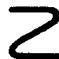
\includegraphics[keepaspectratio]{images/part001_0d60a61e.jpg}}

The definition of Krull dimension is therefore devoid of interest for separated spaces, but it is especially well suited to the topological spaces encountered in Commutative Algebra (spectra of rings, *schemes*, \ldots). In this chapter, no confusion is to be feared with other notions of dimension for topological spaces (for example, that of Lebesgue), and we will simply say “dimension” for “Krull dimension.”

PROPOSITION 1. --- Let X be a topological space.

\begin{enumerate}
\def\labelenumi{\alph{enumi})}
\item
  If Y is a subspace of X, we have \(\dim(\mathbf{Y}) \leqslant \dim(\mathbf{X})\) , and \(\dim_y(\mathbf{Y}) \leqslant \dim_y(\mathbf{X})\) for every point \(y\) of Y.
\item
  Let \(x\) be a point of \(X\) and \(V\) a neighborhood of \(x\) in \(X\) . We have \(\dim_x(X) = \dim_x(V)\) .
\item
  Let \((\mathbf{X}_i)_{i\in I}\) be a finite family of closed subsets of X such that \(\mathbf{X} = \bigcup_{i\in I}\mathbf{X}_i\) . We have
\end{enumerate}

\(\dim(X) = \sup_{i \in I} \dim(X_i)\)and, for every point \(x\) of \(X\)\(\dim_x(X) = \sup_{i \in J_x} \dim_x(X_i)\)\(J\)\(i \in J\)\(x \in X\) , one has

where  denotes the set of  such that .\[
\mathrm{J} _ {x}
\]

Let us prove a). If Z is an irreducible closed subset of Y, its closure \(\overline{Z}\) in X is irreducible (II, § 4, no. 1, prop. 2) and one has \(\overline{Z} \cap Y = Z\) . Thus, every chain \(c\) of closed irreducible subsets of Y defines, by passing to the closure in X, a chain of closed irreducible subsets of X, of the same length as \(c\) . The inequality \(\dim(Y) \leqslant \dim(X)\) follows from this. If U is an open subset of X containing a point \(y\) of Y, we therefore have \(\dim(U \cap Y) \leqslant \dim(U)\) , whence \(\dim_y(Y) \leqslant \dim_y(X)\) .

We prove \(b\) . By definition \(\dim_{x}(X) \leqslant \dim_{x}(V)\) , and the opposite inequality follows from \(a\) ).

We prove \(c\) ). Let \(Z_{0} \subset \ldots \subset Z_{n}\) be a chain of irreducible closed subsets of X. We have \(Z_{n} = \bigcup_{i \in I} (Z_{n} \cap X_{i})\) and each of the sets \(Z_{n} \cap X_{i}\) is closed in \(Z_{n}\) ;

since I is finite, \(Z_{n}\) is contained in one of the \(X_{i}\) . Consequently, we have \(\dim(X) \leqslant \sup_{i} \dim(X_{i})\) , whence equality by \(a\) ).

Now let \(x\) be a point of \(X\) and \(n = \sup_{i \in J_x} \dim_x(X_i)\) , where \(J_x\) is as in the statement. We have \(\dim_x(X) \geqslant n\) by \(a\) ), and, to establish the equality, we may assume \(n\) finite. For every \(i \in J_x\) , let \(U_i\) be an open neighborhood of \(x\) in \(X\) such that \(\dim(U_i \cap X_i) \leqslant n\) . Put \(U = (\bigcap_{i \in J_x} U_i) \cap (\bigcap_{i \in I - J_x} \complement X_i)\) ; the set \(U\) is open in \(X\) . Moreover, we have \(\dim(U) = \sup_{i \in J_x} \dim(U \cap X_i) \leqslant n\) by the preceding paragraph, hence \(\dim_x(X) \leqslant n\) .

COROLLARY. --- a) The dimension of the topological space X is the supremum of the dimensions of its irreducible components (II, § 4, no. 1, definition 2).

\begin{enumerate}
\def\labelenumi{\alph{enumi})}
\setcounter{enumi}{1}
\tightlist
\item
  Let \(x\) be a point of \(X\) . We have \(\dim_x(X) \geqslant \sup_i \dim_x(X_i)\) , where \(X_i\) runs through the family
\end{enumerate}
of irreducible components of X that contain x; there is equality if x has a neighborhood V which has only finitely many irreducible components (which is the case for example if V is Noetherian).


The first assertion is immediate since the chains of irreducible closed subsets of X are the chains of irreducible closed subsets of the irreducible components of X (II, § 4, no. 1, prop. 5). The inequality \(\dim_x(X) \geqslant \sup_i \dim_x(X_i)\) follows

from prop. 1, a). Let V be a neighborhood of x which has only finitely many irreducible components, and let \((\mathrm{V}_{j})_{j\in\mathbb{J}}\) be the family of irreducible components of V that contain x. It follows from prop. 1, b) and c) that we have

\[
\dim_ {x} (X) = \dim_ {x} (V) = \sup _ {j \in J} \dim_ {x} (V _ {j});
\]

we conclude by noting that each of the \(V_{j}\) is contained in one of the \(X_{i}, i \in J_{x}\) , and that consequently we have \(\sup_{j \in J} \dim_{x}(V_{j}) \leqslant \sup_{i \in J_{x}} \dim_{x}(X_{i})\) .

PROPOSITION 2. — Let X be a topological space. We have \(\dim(X) = \sup_{x \in X} \dim_x(X)\) .

Indeed, by definition we have \(\dim(X) \geqslant \dim_x(X)\) for every \(x \in X\) . On the other hand, if \(Z_0 \subset \ldots \subset Z_n\) is a chain of irreducible closed subsets of \(X\) , for all \(x \in Z_0\) and every open neighborhood \(U\) of \(x\) , the sets \(Z_0 \cap U, \ldots, Z_n \cap U\) form a chain of irreducible closed subsets of \(U\) (II, § 4, no. 1, prop. 7). We therefore have \(\dim_x(X) \geqslant n\) , whence \(\dim(X) \leqslant \sup_{x \in X} \dim_x(X)\) .

COROLLARY. — If \((\mathrm{X}_{\alpha})_{\alpha\in\mathbf{A}}\) is an open covering, or a locally finite closed covering, of a topological space X, we have

\[
\dim (X) = \sup _ {\alpha \in A} \dim (X _ {\alpha}).
\]

It suffices to show that, for every point \(x\) of \(X\), one has \(\dim_x(X) = \sup_{\alpha \in A_x} \dim_x(X_\alpha)\), where \(A_x\) is the set of \(\alpha \in A\) such that \(x \in X_\alpha\). This is clear in the case of an open covering, and follows from Proposition 1, c), in the case of a locally finite closed covering.

\subsection{Codimension of a closed subset}

DEFINITION 3. --- Let X be a topological space.

\begin{enumerate}
\def\labelenumi{\alph{enumi})}
\item
  If Y is a closed irreducible subset of X, one calls the codimension of Y in X the supremum in \(\overline{\mathbf{R}}\) of the lengths of the chains of irreducible closed subsets of X for which Y is the smallest element.
\item
  If Y is a closed subset of X, we call the codimension of Y in X, and denote it by \(\text{codim}(Y, X)\) the infimum in \(\overline{\mathbf{R}}\) of the codimensions, in X, of the irreducible components of Y.
\end{enumerate}

Remarks. --- 1) The codimension of a closed subset Y of X is therefore the infimum of the codimensions of the irreducible closed subsets of Y. We have \(\mathrm{codim}(\emptyset, \mathrm{X}) = +\infty\) and, if X is nonempty, \(\mathrm{codim}(\mathrm{X}, \mathrm{X}) = 0\) . Every nonempty closed subset of X contains an irreducible closed subset (II, § 4, no. 1, prop. 5); hence the codimension in X of a closed subset Y is always a nonnegative integer, or \(+\infty\) . It is zero if and only if Y contains an irreducible component of X.

\begin{enumerate}
\def\labelenumi{\arabic{enumi})}
\setcounter{enumi}{1}
\tightlist
\item
  If Y is a nonempty closed subset of X, then codim(Y, X) ≤ dim(X). Moreover, dim(X) = sup codim(Y, X), where Y ranges over the set of irreducible closed subsets.
\end{enumerate}

If Y and Y' are two closed subsets of X such that Y' ⊂ Y, then codim(Y, X) ≤ codim(Y', X).

\begin{enumerate}
\def\labelenumi{\arabic{enumi})}
\setcounter{enumi}{2}
\tightlist
\item
  Let Y be a closed subset of the topological space X and \((\mathrm{X}_{\alpha})_{\alpha\in\mathrm{A}}\) (resp. \((\mathrm{Y}_{\beta})_{\beta\in\mathrm{B}}\) ) the family of irreducible components of X (resp. of Y). For every \(\beta\in B\) , denote by \(\mathrm{A}(\beta)\) the set of \(\alpha\in A\) such that \(Y_{\beta}\subset X_{\alpha}\) . Since every irreducible subset of X is contained in one of the \(X_{\alpha}\) (II, § 4, no. 1, prop. 5), it follows from Def. 3 that we have:
\end{enumerate}

\[
\operatorname{codim} (Y, X) = \inf _ {\beta \in B} \sup _ {\alpha \in A (\beta)} \operatorname{codim} (Y _ {\beta}, X _ {\alpha}).
\]

\begin{enumerate}
\def\labelenumi{\arabic{enumi})}
\setcounter{enumi}{3}
\tightlist
\item
  Let \((\mathbf{Y}_i)_{i\in I}\) be a finite family of closed subsets of X and \(\mathbf{Y} = \bigcup_{i\in I}\mathbf{Y}_i\) ; one has
\end{enumerate}

\[
\operatorname{codim} (\mathrm{Y}, \mathrm{X}) = \inf _ {i \in \mathrm{I}} \operatorname{codim} (\mathrm{Y} _ {i}, \mathrm{X}).
\]

Indeed, every irreducible component of Y is contained in one of the \(Y_{i}\) .

PROPOSITION 3. --- Let X be a topological space.

\begin{enumerate}
\def\labelenumi{\alph{enumi})}
\tightlist
\item
  For every nonempty closed subset Y of X, we have
\end{enumerate}

\[
\dim (\mathrm{Y}) + \operatorname{codim} (\mathrm{Y}, \mathrm{X}) \leqslant \dim (\mathrm{X}).
\]

\begin{enumerate}
\def\labelenumi{\alph{enumi})}
\setcounter{enumi}{1}
\tightlist
\item
  If Y, Z, and T are closed subsets of X such that Y ⊂ Z ⊂ T, then
\end{enumerate}

\[
\operatorname{codim} (\mathrm{Y}, \mathrm{Z}) + \operatorname{codim} (\mathrm{Z}, \mathrm{T}) \leqslant \operatorname{codim} (\mathrm{Y}, \mathrm{T}).
\]

It suffices to prove the assertion \(a)\) in the case where \(\dim(X)\) is finite. In this case, \(\dim(Y)\) and \(\operatorname{codim}(Y, X)\) are finite. There exists a chain \(Y_0 \subset \ldots \subset Y_n\) of closed irreducible subsets of \(Y\), of length \(n = \dim(Y)\) and a chain \(Y_n \subset \ldots \subset Y_{n+p}\) of closed irreducible subsets of \(X\), of length \(p \geqslant \operatorname{codim}(Y, X)\). It follows that \(\dim(X) \geqslant n + p\), whence . To establish \(a)\)\(b)\), one may assume \(Y\) irreducible. Since we have \(\operatorname{codim}(Y, Z) \leqslant \operatorname{codim}(Y, T)\), the inequality is proved if \(\operatorname{codim}(Y, Z) = +\infty\). Otherwise, let \(Z_0\) be an irreducible component of \(Z\) containing \(Y\) and such that \(\operatorname{codim}(Y, Z) = \operatorname{codim}(Y, Z_0)\). We have \(\operatorname{codim}(Z, T) \leqslant \operatorname{codim}(Z_0, T)\), and one sees, as above, that \(\operatorname{codim}(Y, Z_0) + \operatorname{codim}(Z_0, T) \leqslant \operatorname{codim}(Y, T)\), whence \(b)\).

DEFINITION 4. --- A topological space X is said to be catenary if, for every pair (Y, Z) of irreducible closed subsets of X such that Y ⊂ Z, every saturated chain of irreducible closed subsets with endpoints Y and Z has length codim(Y, Z).

It is equivalent to say that, for every pair (Y, Z) of irreducible closed subsets of X such that codim(Y, Z) is finite, all saturated chains with endpoints Y and Z have the same length, and that, for every pair (Y, Z) such that codim(Y, Z) = +∞, there exists no saturated chain with endpoints Y and Z.

Every closed subspace of a catenary space is catenary. For a space to be catenary, it is necessary and sufficient that its irreducible components be catenary.

PROPOSITION 4. --- Let X be a topological space. For X to be catenary, it is necessary and sufficient that, for every triple (Y, Z, T) of irreducible closed subsets of X such that Y ⊂ Z ⊂ T, one has:

\[
\operatorname{codim} (\mathrm{Y}, \mathrm{T}) = \operatorname{codim} (\mathrm{Y}, \mathrm{Z}) + \operatorname{codim} (\mathrm{Z}, \mathrm{T}).
\]

Suppose X is catenary. In view of prop. 3, b), it suffices to prove the relation when codim(Y, Z) and codim(Z, T) are finite. By concatenating a saturated chain of irreducible closed subsets with endpoints Y and Z, of length codim(Y, Z), and a saturated chain of irreducible closed subsets with endpoints Z and T, of length codim(Z, T), one obtains a saturated chain with endpoints Y and T, of length codim(Y, Z) + codim(Z, T). But, since X is catenary, this length is necessarily equal to codim(Y, T).

Conversely, suppose we have \(\operatorname{codim}(\mathbf{Y},\mathbf{T})=\operatorname{codim}(\mathbf{Y},\mathbf{Z})+\operatorname{codim}(\mathbf{Z},\mathbf{T})\) for all irreducible closed subsets  of  such that \(\mathbf{Y}\subset\mathbf{Z}\subset\mathbf{T}\), and let us prove that X is catenary. To do this, we prove by induction on the integer \(n\geqslant0\) that, for every saturated chain \(Z_{0}\subset\ldots\subset Z_{n}\) of closed irreducible subsets of X, we have \(\operatorname{codim}(Z_{0},Z_{n})=n\). If \(n=0\), it is clear. Let \(n>0\), and suppose the property is satisfied for chains of length \(\leqslant n-1\). If \(Z_{0}\subset\ldots\subset Z_{n}\) is a saturated chain of length \(n\), then \(Z_{0}\subset\ldots\subset Z_{n-1}\) is a saturated chain of length \(n-1\), hence \(\operatorname{codim}(Z_{0},Z_{n-1})=n-1\). In view of the hypothesis made on X, we have \(\operatorname{codim}(Z_{0},Z_{n})=\operatorname{codim}(Z_{0},Z_{n-1})+\operatorname{codim}(Z_{n-1},Z_{n})=(n-1)+1=n\).

COROLLARY. — Let X be an irreducible topological space of finite dimension. For X to be catenary, it is necessary and sufficient that, for every pair (Y, Z) of irreducible closed subsets of X such that Y ⊂ Z, one has codim(Y, X) = codim(Y, Z) + codim(Z, X).

The condition is necessary by prop. 4. Conversely, suppose it is satisfied, and denote by \(c(Z)\) the integer \(\operatorname{codim}(Z,X)\) for every irreducible closed subset \(Z\) of \(X\) . If \(Y,Z,T\) are three irreducible closed subsets of \(X\) such that \(Y\subset Z\subset T\) , one has

\[
\begin{array}{r l} \operatorname{codim} (\mathrm{Y}, \mathrm{Z}) + \operatorname{codim} (\mathrm{Z}, \mathrm{T}) & = (c (\mathrm{Y}) - c (\mathrm{Z})) + (c (\mathrm{Z}) - c (\mathrm{T})) \\ & = c (\mathrm{Y}) - c (\mathrm{T}) \\ & = \operatorname{codim} (\mathrm{Y}, \mathrm{T}), \end{array}
\]

and X is catenary by prop. 4.

PROPOSITION 5. — Let X be a topological space of finite dimension. Suppose that all maximal chains of irreducible closed subsets of X have the same length. Then X is catenary; for every irreducible closed subset Z of X, one has

\[
\operatorname{codim} (Z, X) = \dim (X) - \dim (Z);
\]

for every pair (Y, Z) of irreducible closed subsets of X such that Y ⊂ Z, one has

\[
\operatorname{codim} (\mathrm{Y}, \mathrm{Z}) = \dim (\mathrm{Z}) - \dim (\mathrm{Y}).
\]

Let Y and Z be two irreducible closed subsets of X such that \(Y \subset Z\) . Let \(Y_{0} \subset \ldots \subset Y_{p}\) be a chain such that \(Y_{p} = Y\) and \(p = \dim(Y)\) , \(Z_{0} \subset \ldots \subset Z_{q}\) be a chain such that \(Z_{0} = Z\) and \(q = \text{codim}(Z, X)\) . For every saturated chain \(T_{0} \subset \ldots \subset T_{r}\) such that \(T_{0} = Y\) and \(T_{r} = Z\) , the chain

\[
\mathrm{Y} _ {0} \subset \dots \subset \mathrm{Y} _ {p - 1} \subset \mathrm{T} _ {0} \subset \dots \subset \mathrm{T} _ {r} \subset \mathrm{Z} _ {1} \dots \subset \mathrm{Z} _ {q}
\]

is maximal, and of length \(p + q + r\) ; by the hypothesis made on X, one therefore has \(p + q + r = \dim(X)\) . Let \(r = \dim(X) - \dim(Y) - \text{codim}(Z, X)\) . It follows that X is catenary and that, for Y and Z as above, one has

\[
\dim (\mathrm{Y}) + \operatorname{codim} (\mathrm{Y}, \mathrm{Z}) = \dim (\mathrm{X}) - \operatorname{codim} (\mathrm{Z}, \mathrm{X}).
\]

Taking Y = Z, one sees that the second member is equal to dim(Z), whence the proposition.

\subsection{Dimension of a ring, height of an ideal}

DEFINITION 5. — The Krull dimension, or simply the dimension, of a (commutative) ring A is the Krull dimension of the topological space , and is denoted by  (II, § 4, no. 3, definition 4). If  is a prime ideal of A, the dimension of A at \_ is denoted by , namely \_.

The map \(\mathfrak{p} \mapsto \mathrm{V}(\mathfrak{p})\) is a decreasing bijection from the set of prime ideals of A onto the set of irreducible closed subsets of \(\operatorname{Spec}(A)\) (loc. cit., cor. 2 to prop. 14). The dimension of A is therefore the supremum of the set of lengths of chains of prime ideals of A; it is equal to \(-\infty\) , \(+\infty\) or to a positive integer.

Let \(\mathfrak{p} \in \operatorname{Spec}(\mathbf{A})\); the sets \(\operatorname{Spec}(\mathbf{A})_f\), as \(f\) ranges over A, form a basis for the topology of \(\operatorname{Spec}(\mathbf{A})\), and \(\mathfrak{p}\) belongs to the open set \(\operatorname{Spec}(\mathbf{A})_f\) if and only if \(f\) does not belong to \(\mathfrak{p}\). Consequently, \(\dim_{\mathfrak{p}}(\mathbf{A})\) is the infimum of the numbers \(\dim(\mathbf{A}_f)\), where \(f\) ranges over \(\mathfrak{p}\) (II, § 5, no. 1, Proposition 1).

Examples. --- 1) We have  if and only if A is reduced to 0. For \textless to hold, it is necessary and sufficient that every prime ideal of A be maximal. The integral domains of dimension 0 are the fields. A Noetherian ring has dimension {} if and only if it is Artinian (IV, § 2, no. 5, prop. 9).

\begin{enumerate}
\def\labelenumi{\arabic{enumi})}
\setcounter{enumi}{1}
\item
  Dedekind rings are the Noetherian integrally closed rings of dimension \(\leqslant 1\) (VII, § 2, no. 2, th. 1). More generally, by V, § 1, no. 2, cor. 2 to prop. 9, a ring is a finite product of Dedekind rings if and only if it is Noetherian, reduced, integrally closed in its total ring of fractions, and of dimension \(\leqslant 1\) .
\item
  If A is a valuation ring (VI, § 1, No. 2, Def. 2), its dimension is equal to the height of the valuation (VI, § 4, No. 4, Prop. 5).
\item
  Let A be a ring. We have
\end{enumerate}

\[
\dim (\mathrm{A} [ \mathrm{X} ]) \geqslant \dim (\mathrm{A}) + 1.
\]

Indeed, if \(\mathfrak{p}_0 \subset \ldots \subset \mathfrak{p}_n\) is a chain of prime ideals of A, of length \(n\) , we obtain a chain \(\mathfrak{p}_0' \subset \ldots \subset \mathfrak{p}_{n+1}'\){}{} of prime ideals of A[X], of length \(n+1\) , by setting \(\mathfrak{p}_i' = \mathfrak{p}_iA[X]\) for \(0 \leqslant i \leqslant n\) , and \(\mathfrak{p}_{n+1}' = \mathfrak{p}_nA[X] + XA[X]\) .

By the same reasoning, one proves the inequality \(\dim(\mathrm{A}[[\mathrm{X}]]) \geqslant \dim(\mathrm{A}) + 1\) . From this one deduces by induction the inequalities

\[
\begin{array}{l} \dim (\mathrm{A} [ \mathrm{X} _ {1},..., \mathrm{X} _ {n} ]) \geqslant \dim (\mathrm{A}) + n, \\ \dim (\mathrm{A} [ [ \mathrm{X} _ {1},..., \mathrm{X} _ {n} ] ]) \geqslant \dim (\mathrm{A}) + n. \end{array}
\]

We shall show later (§ 3, no. 4, cor. 3 of prop. 7 and cor. 3 of prop. 8) that equality holds in the two preceding formulas when A is Noetherian.

* 5) Let X be a complex analytic manifold. If X has complex dimension n at a point x of X, the local ring of germs at x of analytic functions on X has dimension n.*

\begin{enumerate}
\def\labelenumi{\arabic{enumi})}
\setcounter{enumi}{5}
\item
  Let \(k\) be a field and A a nonzero integral \(k\)-algebra. Then one has \(\dim(A) = 0\) . This follows from cor. 1 of prop. 1 of V, § 2, no. 1, and from the fact that \(\dim(k) = 0\) .
\item
  If n is a nilideal of A, Spec(A) is homeomorphic to Spec(A/n) (II, § 4, no. 3, remark). Hence one has dim(A/n) = dim(A); in particular, one has dim(A) = dim(A\(_{red}\)) where A\(_{red}\) is the quotient of the ring A by its nilradical.
\item
  There exist Noetherian rings of infinite dimension (p. 83, exerc. 13). We shall see below (§ 3, no. 1, cor. 1 of prop. 2) that every Noetherian local ring has finite dimension.
\end{enumerate}

PROPOSITION 6. --- Let A be a ring.

\begin{enumerate}
\def\labelenumi{\alph{enumi})}
\item
  If \(\mathfrak{a}\) is an ideal of A, one has \(\dim (\mathrm{A} / \mathfrak{a})\leqslant \dim (\mathrm{A}).\)
\item
  If S is a multiplicative subset of A, one has \(\dim (\mathbf{S}^{-1}\mathbf{A})\leqslant \dim (\mathbf{A}).\)
\item
  We have \(\dim(A) = \sup_{\mathfrak{p}} \dim(A/\mathfrak{p})\) , where \(\mathfrak{p}\) runs through the set of minimal prime ideals of A.
\item
  If A has only finitely many minimal prime ideals (for example if A is Noetherian (II, § 4, no. 3, Corollary 3 to Proposition 14)) and if \(\mathfrak{p}\) is a prime ideal of A, one has
\end{enumerate}

\[
\dim_ {\mathfrak {p}} (\mathrm{A}) = \sup _ {\mathfrak {q}} \dim_ {\mathfrak {p} / \mathfrak {q}} (\mathrm{A} / \mathfrak {q}),
\]

where \(\mathfrak{q}\) runs through the set of minimal prime ideals of A contained in \(\mathfrak{p}\).

\begin{enumerate}
\def\labelenumi{\alph{enumi})}
\setcounter{enumi}{4}
\tightlist
\item
  Let  be an ideal of A which is contained in no minimal prime ideal of A; one then has . In particular, if A is an integral domain, one has  for every nonzero ideal  of A.
\end{enumerate}

By the remark in II, § 4, no. 3, if  is an ideal of A, the topological space  is homeomorphic to the closed subspace  of . Assertion  follows from this and from Proposition 1, a), of no. 1. Assertion  follows from loc. cit., the corollary to Proposition 13. By loc. cit., Corollary 2 to Proposition 14, the irreducible components of  are homeomorphic to the spaces , where  is a minimal prime ideal of A, and assertion  follows from the corollary of Proposition 1 of no. 1. Under the hypothesis of , the space  has only finitely many irreducible components; the irreducible components of  containing  are the sets , where  is a minimal prime ideal contained in . Assertion  then follows from the corollary, b), of Proposition 1 of no. 1.

Let us finally prove \(e\) ). We need to prove that, for any chain \(\mathfrak{p}_{0} \subset \ldots \subset \mathfrak{p}_{n}\) of prime ideals of A such that \(\mathfrak{a} \subset \mathfrak{p}_{0}\) , one has \(\dim(A) \geqslant n + 1\) . In view of the hypothesis made on \(\mathfrak{a}\) there exists a prime ideal \(\mathfrak{p}_{-1}\) of A contained in \(\mathfrak{p}_{0}\) , distinct from \(\mathfrak{p}_{0}\) , and \(\mathfrak{p}_{-1} \subset \mathfrak{p}_{0} \subset \ldots \subset \mathfrak{p}_{n}\) is a chain of prime ideals of A, of length \(n + 1\) .

Remark 1. --- Let \(\rho: A \to B\) be a ring homomorphism. Then  is the supremum of the numbers , where \(\rho(p)\) ranges over the set of minimal prime ideals of A: indeed, for every minimal prime ideal \(p\) of B, there exists a minimal prime ideal \(q\) of A contained in \(\mathfrak{p}\)\(\rho^{-1}(\mathfrak{q})\) (II, § 2, no. 6, lemma 2), and one has

\[
\dim (\mathbf {B} / \mathfrak {q}) \leqslant \dim (\mathbf {B} / \rho (\mathfrak {p})\mathbf {B}) \leqslant \dim (\mathbf {B})
\]

By prop. 6, a); we conclude by prop. 6, c).

DEFINITION 6. --- Let  be an ideal of a ring A. The codimension of  in  is called the height of the ideal  and is denoted by .

Suppose A is integral. Then the prime ideals of height 1 of A in the sense of def. 4 of VII, § 1, no. 6 are precisely the prime ideals of height 1 in the sense of the definition above.

PROPOSITION 7. --- a) The height of a prime ideal  of A is the supremum of the lengths of chains of prime ideals \(\mathfrak{p}_{0} \subset \ldots \subset \mathfrak{p}_{n}\) such that \(\mathfrak{p}_{n} = \mathfrak{p}\).

\begin{enumerate}
\def\labelenumi{\alph{enumi})}
\setcounter{enumi}{1}
\item
  Let  be a prime ideal of A and  an ideal of A. Then we have  if  is not contained in \(\dim(A_{p}/\mathfrak{a}A_{p}) = -\infty\) and  if  is contained in \(\dim(A_{p}/\mathfrak{a}A_{p}) = \text{codim}(V(p), V(a))\) . In particular, if  is a prime ideal of A, one has \(\dim(A_{\mathfrak{p}}) = \operatorname{ht}(\mathfrak{p})\) .
\item
  If  is an ideal of A, one has , where  ranges over the set of prime ideals of A containing \_.
\end{enumerate}

The assertion  is the translation of Definition 3, , of no. 2. The assertion  follows from the fact that the map  is an order-preserving isomorphism of the set of prime ideals  of A such that  onto the set of prime ideals of the local ring  (II, § 2, no. 5, Proposition 11). Let  be an ideal of A; the irreducible closed subsets of  are the sets , where  is a prime ideal of A containing . Assertion  therefore follows from Remark 1 of no. 2.

\(a\)\(a\)\(b\)\(\mathfrak{q} \mapsto \mathfrak{q}(A_{\mathfrak{p}} / aA_{\mathfrak{p}})\)\(\mathfrak{q}\)\(\mathfrak{a} \subset \mathfrak{q} \subset \mathfrak{p}\)\(A_{\mathfrak{p}} / aA_{\mathfrak{p}}\)\(\mathfrak{a}\)\(\mathfrak{a}\)COROLLARY. --- Let \(\mathfrak{p}\) be a prime ideal of A and S a multiplicative subset of A not meeting \(\mathfrak{p}\). Then \(\mathfrak{a}\)\(c\)

\(^{-1}\).

This follows from prop. 7, a), and II, § 2, no. 5, prop. 11.

PROPOSITION 8. --- Let A be a ring.

\begin{enumerate}
\def\labelenumi{\alph{enumi})}
\item
  We have  , where \(\dim(A) = \sup_{\mathfrak{m}} \dim(A_{\mathfrak{m}}) = \sup_{\mathfrak{m}} \operatorname{ht}(\mathfrak{m})\)\(m\)\(A\) runs through the set of maximal (resp. prime) ideals of A.
\item
  Let  be an ideal of A distinct from A and let  be an ideal of A contained in . Then we have  . In particular, for every ideal  of A distinct from A, we have the inequality .
\end{enumerate}

The first assertion follows from remark 2 of no. 2 and from prop. 7, b). The second follows from prop. 3, a) of no. 2 and from the relations , .

DEFINITION 7. --- A ring A is said to be catenary if the topological space Spec(A) is catenary (no. 2, def. 4).

This means therefore that, for every pair \((\mathfrak{p}, \mathfrak{q})\) of prime ideals of A such that \(\mathfrak{q} \subset \mathfrak{p}\) , all saturated chains of prime ideals of A with endpoints \(\mathfrak{p}\) and \(\mathfrak{q}\) have length \(\operatorname{codim}(\mathrm{V}(\mathfrak{p}), \mathrm{V}(\mathfrak{q})) = \dim(\mathrm{A}_{\mathfrak{p}} / \mathfrak{q}\mathrm{A}_{\mathfrak{p}})\) .

Remarks. --- 2) Every quotient ring of a catenary ring is catenary. For the ring A to be catenary, it is necessary and sufficient that, for every prime ideal  of A, the ring \(\mathfrak{p}\) be catenary.

\begin{enumerate}
\def\labelenumi{\arabic{enumi})}
\setcounter{enumi}{2}
\item
  By prop. 7, b) and prop. 4 of no. 2, the ring A is catenary if and only if, for every triple  of prime ideals of A such that , we have \(\dim(A_{p}/qA_{p}) + \dim(A_{q}/rA_{q}) = \dim(A_{p}/rA_{p})\) . If A is integral and of finite dimension, then A is catenary if and only if we have \(ht(q) + \dim(A_{p}/qA_{p}) = ht(p)\) for every pair  of prime ideals of A such that \((p, q)\)\(\mathfrak{q} \subset \mathfrak{p}\) . Indeed, the topological space Spec(A) is then irreducible and of finite dimension, and we apply the corollary to prop. 4 of no. 2.
\item
  Let A be a ring of finite dimension, all of whose maximal chains of prime ideals have the same length. Then A is catenary, we have  for every prime ideal  of A, and  for every pair \_ of prime ideals of A such that \_ (no. 2, prop. 5).
\item
  We shall see in § 2, no. 4, that every algebra of finite type over a field is a catenary ring. There exist local noetherian rings which are not catenary (p. 83, exerc. 16).
\end{enumerate}

\subsection{Dimension of a finitely generated module}

DEFINITION 8. — Let A be a ring and M a finitely generated A-module. One calls the Krull dimension (or simply the dimension \(^{1}\)) of the A-module M and denotes it by  (or \(_{A}\) if there is no ambiguity), the Krull dimension of the support of M (II, § 4, no. 4, def. 5).

The support of the A-module A is Spec(A); the dimension of the A-module A is therefore equal to the dimension of the ring A.

Let M be a finitely generated A-module and  its annihilator; one has

\[
\operatorname{Supp} (\mathbf {M}) = \mathrm{V} (\mathfrak {a}) = \operatorname{Supp} (\mathrm{A} / \mathfrak {a})
\]

(II, § 4, no. 4, prop. 17). Consequently the dimension of the A-module M, the dimension of the A-module , the dimension of the ring , and the dimension of the -module M coincide; it is the supremum of the set of lengths of chains  of prime ideals of A such that \(p_0 \subset \ldots \subset p_n\) . By prop. 6, c) of no. 3, the dimension of M is also the supremum of the dimensions of the rings (or of the A-modules) , where  ranges over the set of prime ideals of A which are minimal among those containing \(a \subset p_0\).

Remarks. — 1) Let A be a noetherian ring and M a finitely generated A-module. It is equivalent to say that dim \(_{A}\) (M) ≤ 0, or that the elements of Supp(M) are maximal ideals of A, or that M is of finite length (IV, § 2, no. 5, prop. 7).

\begin{enumerate}
\def\labelenumi{\arabic{enumi})}
\setcounter{enumi}{1}
\tightlist
\item
  If M is a finitely generated module over a noetherian ring A, \(\dim_{\mathrm{A}}(\mathrm{M})\) is the supremum of the numbers \(\dim(\mathrm{A}/\mathfrak{p})\) , where  ranges over the set \(\operatorname{Ass}_{\mathrm{A}}(\mathrm{M})\) of prime ideals of A associated with M (IV, § 1, no. 4, th. 2).
\end{enumerate}

PROPOSITION 9. — Let A be a ring and M a finitely generated A-module.

\begin{enumerate}
\def\labelenumi{\alph{enumi})}
\item
  For every \(\mathfrak{p} \in \operatorname{Supp}(\mathbf{M})\) , one has \(\dim_{\mathbf{A}_{\mathfrak{p}}}(\mathbf{M}_{\mathfrak{p}}) = \operatorname{codim}(\mathbf{V}(\mathfrak{p}), \operatorname{Supp}(\mathbf{M}))\) .
\item
  \(\dim_{\mathbf{A}}(\mathbf{M})\) is the least upper bound of the \(\dim_{\mathbf{A}_{\mathfrak{p}}}(\mathbf{M}_{\mathfrak{p}})\) , where \(\mathfrak{p}\) ranges over \(\operatorname{Spec}(\mathbf{A})\) (resp. where \(\mathfrak{p}\) ranges over the set of maximal ideals of A belonging to \(\operatorname{Supp}(\mathbf{M})\) ).
\item
  Let \(\mathbf{M}'\) be a finitely generated submodule of \(\mathbf{M}\) ; then
\end{enumerate}

\[
\dim_ {\mathrm{A}} (\mathrm{M}) = \sup \left(\dim_ {\mathrm{A}} \left(\mathrm{M} ^ {\prime}\right), \dim_ {\mathrm{A}} \left(\mathrm{M} / \mathrm{M} ^ {\prime}\right)\right).
\]

\begin{enumerate}
\def\labelenumi{\alph{enumi})}
\item
  Let  be the annihilator of M; then the annihilator of the \(_{p}\)-module \(_{p}\) is \(_{p}\)\(_{A_{p}}\) (II, § 2, no. 4, formula (9)), whence \(_{p}\)\(_{p}\)\(_{p}\) . We conclude by prop. 7, b) of no. 3.
\item
  This follows immediately from  and the fact that  if  does not belong to \(\dim_{\mathrm{A}_{\mathfrak{p}}}(M_{\mathfrak{p}}) = -\infty\).
\item
  We have \(\operatorname{Supp}(\mathbf{M}) = \operatorname{Supp}(\mathbf{M}') \cup \operatorname{Supp}(\mathbf{M} / \mathbf{M}')\) (II, §4, no. 4, prop. 16), and one applies prop. 1 of no. 1.
\end{enumerate}

Remark 3. --- Under the conditions of Prop. 9, c), one has codim(Supp(M), Spec(A)) = inf(codim(Supp(M'), Spec(A)), codim(Supp(M/M'), Spec(A))). This follows from the formula Supp(M) = Supp(M') ∪ Supp(M/M') and from Remark 4 of no. 2.

\subsection{Cycles associated with a module}

In this number, we denote by A a Noetherian ring.

{}{}Let Z(A) be the free Z-module with basis the set of irreducible closed subsets of Spec(A); for every irreducible closed subset Y of Spec(A), we denote by [Y] the corresponding element of Z(A). The elements of Z(A) are sometimes called cycles.

Let M be a finitely generated A-module. For every prime ideal  of A which is a minimal element of , we have \(0 < \text{long}_{A_{p}}(M_{p}) < \infty\) (IV, § 2, no. 5, Corollary 2 to Proposition 7 and § 1, no. 4, theorem 2); we set

\[
z (\mathbf {M}) = \sum_ {\mathfrak {p}} \operatorname{long} _ {\mathrm{A} _ {\mathfrak {p}}} (\mathrm{M} _ {\mathfrak {p}}). [ \mathrm{V} (\mathfrak {p}) ],
\]

where  ranges over the finite set of minimal prime ideals of Supp(M).

Remark. --- For every \(\mathfrak{p} \in \operatorname{Spec}(\mathbf{A})\), one has \(z(\mathbf{A}/\mathfrak{p}) = [\mathbf{V}(\mathfrak{p})]\). More generally, let M be a finitely generated A-module, and let \((\mathbf{M}_i)_{0 \leqslant i \leqslant n}\) be a composition series of M such that, for \(0 \leqslant i \leqslant n - 1\), the module \(\mathbf{M}_i / \mathbf{M}_{i+1}\) is isomorphic to \(\mathbf{A}/\mathfrak{p}_i\), where \(\mathfrak{p}_i\) is a prime ideal of A (cf. IV, § 1, no. 4, theorem 1); then we have \(z(\mathbf{M}) = \sum_{i \in \mathbf{J}} [\mathbf{V}(\mathfrak{p}_i)]\), where  is the subset of I consisting of those \(i\) such that \(\mathfrak{p}_i\) is a minimal element of \(\{\mathfrak{p}_0, \ldots, \mathfrak{p}_{n-1}\}\) (IV, § 1, no. 4, theorem 2 and § 2, no. 5, Remark 1).

For every integer \(d\) , denote by \(Z_{\leq d}\) (resp. \(Z_d\) , respectively \(Z^{\geq d}\) , respectively \(Z^d\) ) the sub-\(\mathbf{Z}\)-module of \(Z(A)\) generated by the elements  where \([V(\mathfrak{p})]\) is a prime ideal of A such that \(\mathfrak{p}\) (resp. \(A\), respectively \(\dim(A/\mathfrak{p}) \leqslant d\), respectively \(\dim(A/\mathfrak{p}) = d\)\(\operatorname{ht}(\mathfrak{p}) \geqslant d\)\(\operatorname{ht}(\mathfrak{p}) = d\)). The elements of \(Z_{d}\) (resp. \(Z^{d}\)) are said to be the cycles of dimension \(d\) (respectively, of codimension \(d\)). We obviously have

\[
\mathbf {Z} _ {\leqslant d} = \mathbf {Z} _ {\leqslant d - 1} \oplus \mathbf {Z} _ {d}, \quad \mathbf {Z} ^ {\geqslant d} = \mathbf {Z} ^ {\geqslant d + 1} \oplus \mathbf {Z} ^ {d}.
\]

Let C be the set of classes of finitely generated A-modules (A, VIII, § 3, no. 5), and for each integer d, let \(C_{\leq d}\) (resp. \(C^{\geq d}\)) be the subset of C consisting of the classes of finitely generated A-modules of dimension \(\leq d\) (resp. whose support has codimension \(\geq d\) in Spec(A)).

Lemma 1. --- Let M be a finitely generated A-module and let d be an integer.

\begin{enumerate}
\def\labelenumi{\alph{enumi})}
\tightlist
\item
  For M to be of type \(C_{\leq d}\) it is necessary and sufficient that \(z(\mathbf{M}) \in \mathbf{Z}_{\leq d}\) ; the projection \(z_{d}(\mathbf{M})\) of \(z(\mathbf{M})\) onto \(Z_{d}\) parallel to \(Z_{\leq d-1}\) is then given by
\end{enumerate}

\[
z _ {d} (\mathrm{M}) = \sum _ {\dim (\mathrm{A} / \mathfrak {p}) = d} \operatorname{long} _ {\mathrm{A} _ {\mathfrak {p}}} (\mathrm{M} _ {\mathfrak {p}}). [ \mathrm{V} (\mathfrak {p}) ].
\]

\begin{enumerate}
\def\labelenumi{\alph{enumi})}
\setcounter{enumi}{1}
\tightlist
\item
  For M to be of type \(C^{\geq d}\) it is necessary and sufficient that \(z(\mathbf{M})\in\mathbf{Z}^{\geq d}\) ; the projection \(z^{d}(\mathbf{M})\) of \(z(\mathbf{M})\) onto \(\mathbf{Z}^{d}\) parallel to \(\mathbf{Z}^{\geq d+1}\) is then given by
\end{enumerate}

\[
z ^ {d} (\mathbf {M}) = \sum _ {\operatorname{ht} (\mathfrak {p}) = d} \operatorname{long} _ {\mathrm{A} _ {\mathfrak {p}}} (\mathrm{M} _ {\mathfrak {p}}). [ \mathrm{V} (\mathfrak {p}) ].
\]

For M to be of type \(C_{\leq d}\), i.e. of dimension \(\leq d\), it is necessary and sufficient that, for every minimal prime ideal  of , one has \(\leq d\), which means that \(z(M) \in Z_{\leq d}\). Suppose that , and let \(\leq d\) such that \(p \in Spec(A)\); then either \(p \notin Supp(M)\), and therefore \(M_p = 0\), or \(p \in Supp(M)\), and { is a minimal element of }; the coefficient of {} in \(z(M)\) is in both cases \(_{A_p}(M_p)\), whence a). Part b) is proved analogously; note that a finitely generated module M is of type \(C^{\geq d}\) if and only if one has  for every prime ideal \(M_{\mathfrak{p}} = 0\) of height \textless{}.

By prop. 9, c) and remark 3 of no. 4, the sets \(\mathcal{C}_{\leq d}\) and \(\mathcal{C}^{\geq d}\) are hereditary (A, VIII, § 10, no. 1, def. 1), and one may consider the Grothendieck groups  and  corresponding to them (loc. cit., no. 2); for every A-module M of finite type in \(\mathcal{C}_{\leq d}\) (resp. \(\mathcal{C}^{\geq d}\)), we denote by  (resp. \(\mathcal{C}_{\leq d}\)\(\mathcal{C}^{\geq d}\){) the associated element in }{}\(_{\leq d}\) (resp. {}{}\(^{\geq d}\)\(\mathcal{C}_{\leq d}\)\(\mathcal{C}^{\geq d}\)). By Lemma 1, the functions \(z_{d}\) and \(z^{d}\) are additive; hence there exist (loc. cit., Prop. 3) homomorphisms

\[
\zeta_ {d}: \mathrm{K} (\mathbb {C} _ {\leqslant d}) \rightarrow Z _ {d}, \quad \zeta^ {d}: \mathrm{K} (\mathbb {C} ^ {\geqslant d}) \rightarrow Z ^ {d}
\]

such that \(\zeta_d([M]_{\leq d}) = z_d(M)\) for every finitely generated A-module of type \(C_{\leq d}\) and \(\zeta^d ([N]^{\geq d}) = z^d (N)\) for every finitely generated A-module N of type \(C^{\geq d}\). Moreover, since \(C_{\leq d-1} \subset C_{\leq d}\) and \(C^{\geq d+1} \subset C^{\geq d}\), we have canonical homomorphisms

\[
i _ {d}: \mathrm{K} (\mathbb {C} _ {\leqslant d - 1}) \rightarrow \mathrm{K} (\mathbb {C} _ {\leqslant d}) \quad \text {\text{ and }} \quad i ^ {d}: \mathrm{K} (\mathbb {C} ^ {\geqslant d + 1}) \rightarrow \mathrm{K} (\mathbb {C} ^ {\geqslant d}).
\]

With these notations:

PROPOSITION 10. --- The sequences of Z-modules and homomorphisms

\[
\mathrm{K} \left(\mathbb {C} _ {\leqslant d - 1}\right) \xrightarrow {i _ {d}} \mathrm{K} \left(\mathbb {C} _ {\leqslant d}\right) \xrightarrow {\zeta_ {d}} \mathrm{Z} _ {d} \longrightarrow 0
\]

\[
\mathrm{K} \left(\mathbb {C} ^ {\geqslant d + 1}\right) \xrightarrow {i ^ {d}} \mathrm{K} \left(\mathbb {C} ^ {\geqslant d}\right) \xrightarrow {\zeta ^ {d}} \mathrm{Z} ^ {d} \longrightarrow 0
\]

are exact.

We have \(\zeta_d \circ i_d = 0\) . By Lemma 1, for every \(\mathfrak{p} \in \operatorname{Spec}(A)\) such that \(\dim(A/\mathfrak{p}) = d\) , one has \(\zeta_d([A/\mathfrak{p}]_{\leq d}) = z_d(A/\mathfrak{p}) = [V(\mathfrak{p})]\) , hence the homomorphism \(\zeta_d\) is surjective. By IV, § 1, no. 4, th. 1, \(K(C_{\leq d})\) is generated by the \([A/\mathfrak{p}]_{\leq d}\) , where \(\mathfrak{p} \in \operatorname{Spec}(A)\) and \(\dim(A/\mathfrak{p}) \leqslant d\) ; consequently, every element \(\xi\) of \(K(C_{\leq d})\) can be written \(\xi = i_d(\eta) + \sum_{i=1}^{k} n_i[A/\mathfrak{p}_i]_{\leq d}\) , with \(\eta \in K(C_{\leq d-1})\) , \(n_i \in Z\) and \(\dim(A/\mathfrak{p}_i) = d\) for \(1 \leqslant i \leqslant k\) ; one has \(\zeta_d(\xi) = \sum_{i=1}^{k} n_i[V(\mathfrak{p}_i)]\) and consequently \(\zeta_d(\xi) = 0\) implies \(\xi = i_d(\eta) \in \operatorname{Im}(i_d)\) , whence \(\operatorname{Ker}(\zeta_d) = \operatorname{Im}(i_d)\) .

One argues similarly for the second sequence.

Examples. --- 1) Suppose A is Noetherian and integral. Then we have \(Z^0 = \mathbf{Z}\){}{} ; one has \(C^{\geqslant 0} = C\) and \(z^0(M) = \operatorname{rg}(M)\) .[Spec(A)]. The modules of type \(C^{\geqslant 1}\) are therefore the torsion modules.

\begin{enumerate}
\def\labelenumi{\arabic{enumi})}
\setcounter{enumi}{1}
\item
  Suppose A is Noetherian and integrally closed. Then \(Z^1\) is identified with the group D(A) of divisors of A introduced in Chapter VII (§ 1, no. 3, th. 2, and no. 6, th. 3). The modules of type \(C^{\geqslant 2}\) are the pseudo-null modules (VII, § 4, no. 4, def. 2); if M is a finitely generated torsion module, then \(z^1(M) \in Z^1 = D(A)\) is the content \(\chi(M)\) of M (VII, § 4, no. 5, def. 4). Props. 10 and 11 of loc. cit. are therefore equivalent to the exactness of the sequence \(K(C^{\geqslant 2}) \to K(C^{\geqslant 1}) \to Z^1 \to 0\) .
\item
  The modules of type \(C_{\leqslant0}\) are the modules of dimension \(\leqslant0\) , that is, the modules of finite length (no. 4, remark 1). We have \(\text{long}_{\mathbf{A}}(\mathbf{M}) = \varepsilon(z_0(\mathbf{M}))\) for every A-module M of finite length, where \(\varepsilon: Z_0 \to Z\) associates to the linear combination \(\sum_{m} n_{m}[V(m)]\) the integer \(\sum_{m} n_{m}\) (IV, § 2, no. 5, corollary to prop. 8).
\item
  Suppose A is integral and of finite dimension. Set \(d = \dim(A)\) . Then one has \(\mathcal{C}_{\leq d} = \mathcal{C}\) , \(Z_d = \mathbf{Z}\){}{}\(Z^0\) , \(z_d(M) = \operatorname{rg}(M)\) . [Spec(A)] = \(z^0(M)\) , and the modules of type \(\mathcal{C}_{\leq d-1}\) are the torsion modules.
\end{enumerate}

\section{DIMENSION OF ALGEBRAS}

\subsection{Dimension and flatness}

Let \(\rho: A \to B\) be a ring homomorphism. We denote by (PM) the following condition:

(PM) There exists a B-module  faithfully flat over A such that, for every prime ideal  of B, one has \(_{B}\).

Remarks. --- 1) Condition (PM) is satisfied when there exists a finitely generated B-module, faithfully flat over A and with support equal to Spec(B). This is the case, in particular, if the A-module B is faithfully flat.

\begin{enumerate}
\def\labelenumi{\arabic{enumi})}
\setcounter{enumi}{1}
\item
  The existence of a B-module  faithfully flat over A implies the injectivity of \(\rho\) (I, § 3, no. 5, Proposition 8), and the surjectivity of the map \({}^{a}\rho : \operatorname{Spec}(B) \to \operatorname{Spec}(A)\) (II, § 2, no. 5, Corollary 4 to Proposition 11).
\item
  Suppose that \(\rho: A \to B\) is a local homomorphism of local rings and that there exists a B-module \(N\) flat over A such that  for every prime ideal \(A\)\(N \otimes_B \kappa(\mathfrak{q}) \neq 0\)\(B\) of B. Then \(N\)\(A\) is faithfully flat over A and \(\rho\) therefore enjoys property (PM): indeed, we have , hence \(N/\mathfrak{m}_{B}N = N \otimes_B \kappa(\mathfrak{m}_{B}) \neq 0\) and a fortiori \(N \neq \mathfrak{m}_{B}N\)\(N \neq \mathfrak{m}_{A}N\), and the conclusion follows from Proposition 1 of I, § 3, no. 1.
\end{enumerate}

PROPOSITION 1. --- Let \(\rho: A \to B\) be a ring homomorphism satisfying condition (PM).

\begin{enumerate}
\def\labelenumi{\alph{enumi})}
\item
  Let \(h: \mathbf{A} \to \mathbf{A}'\) be a ring homomorphism. Then the homomorphism \(\rho': \mathbf{A}' \to \mathbf{A}' \otimes_{\mathbf{A}} \mathbf{B}\) deduced from \(\rho\) satisfies condition (PM).
\item
  Let  be a prime ideal of B and \(^{-1}\). The canonical homomorphism \(_{p}\)\(_{q}\) satisfies condition (PM).
\item
  Let  be a prime ideal of B and \(\mathfrak{p} = \rho^{-1}(\mathfrak{q})\). For every prime ideal  of A contained in , there exists a prime ideal \(\mathfrak{p}'\) of B lying over  and contained in \(\mathfrak{q}'\)\(p'\).
\end{enumerate}

Let  be a B-module faithfully flat over A such that  for every prime ideal \(N \otimes_{B} \kappa(q) \neq 0\) of B.

We prove \(a)\). The A'-module \(\mathbf{N}' = \mathbf{A}' \otimes_{\mathbf{A}} \mathbf{N}\) is faithfully flat (I, § 3, no. 3, Proposition 5); let  be a prime ideal of \(\mathbf{B}' = \mathbf{A}' \otimes_{\mathbf{A}} \mathbf{B}\) and  its inverse image in B. We have isomorphisms

\[
\mathrm{N} ^ {\prime} \otimes_ {\mathrm{B} ^ {\prime}} \kappa (\mathfrak {q} ^ {\prime}) \rightarrow \mathrm{N} \otimes_ {\mathrm{B}} \kappa (\mathfrak {q} ^ {\prime}) \rightarrow (\mathrm{N} \otimes_ {\mathrm{B}} \kappa (\mathfrak {q})) \otimes_ {\kappa (\mathfrak {q})} \kappa (\mathfrak {q} ^ {\prime});
\]

since , we also have \(_{B}\)\(_{B'}\).

Let us prove . By Propositions 13 and 14 of II, § 3, no. 4, the -module \(_{p}\) is flat. On the other hand, let \(_{q}\) be a prime ideal of \(_{q}\); it is of the form , where \(_{q}\) is a prime ideal of B contained in \(\mathfrak{b}\) (II, § 3, no. 1, Proposition 3). We have \(\mathfrak{q}\) by the hypothesis on N, and since  is isomorphic to \(_{q}\), we have \(_{q}\)\(_{q}\). Remark 3 allows us to conclude.

Let us prove c). The local homomorphism \(\rho_{\mathfrak{q}}: \mathrm{A}_{\mathfrak{p}} \to \mathrm{B}_{\mathfrak{q}}\) deduced from \(\rho\) satisfies condition (PM) by b). The map \(\operatorname{Spec}(\mathrm{B}_{\mathfrak{q}}) \to \operatorname{Spec}(\mathrm{A}_{\mathfrak{p}})\) is therefore surjective (remark 2), which is what we wanted to prove.

COROLLARY. --- Let F be a closed subset of Spec(A). If Y is an irreducible component of the inverse image of F under the map , then the closure of \(^{a}\rho : \operatorname{Spec}(B) \to \operatorname{Spec}(A)\)\(^{a}\rho(Y)\) is an irreducible component of F.

Let  be an ideal of A such that  and  the prime ideal of B such that \(F = V(a)\). The inverse image under  of F is the subset \(Y = V(\mathfrak{q})\) of , and the closure of  is the irreducible closed subset \(V(\rho(a)B)\) of \(V(\rho^{-1}(q))\).

We need to prove that if  is minimal among the prime ideals of B containing , then \(\rho(a)\) is minimal among the prime ideals of A containing \(\rho^{-1}(q)\). Otherwise, there would exist a prime ideal \(p'\) of A with  and \(a \subset p' \subset \rho^{-1}(q)\); by prop. 1, c), there would exist a prime ideal \(p' \neq \rho^{-1}(q)\) of B such that \(\mathfrak{q}'\) and , whence \(\mathfrak{q}' \subset \mathfrak{q}\) and \(\mathfrak{p}' = \rho^{-1}(\mathfrak{q}')\), contrary to the hypothesis made on \(\rho(a) \subset q' \subset q\)\(q' \neq q\).

PROPOSITION 2. --- Let  be a homomorphism of nonzero rings possessing property (PM). Then we have the inequality

\[
\dim (\mathbf {B}) \geqslant \dim (\mathbf {A}) + \inf _ {\mathfrak {m} \in \mathbf {S}} \dim (\mathbf {B} / \mathfrak {m B})\tag{1}
\]

where S is the set of maximal ideals of A.

We know that \(\dim(A) = \sup_{\mathfrak m \in S} \dim(A_{\mathfrak m})\)\(\S\)\(n^o\) (§ 1, no. 3, Proposition 8). It therefore suffices to establish the inequality

\[
\dim (\mathbf {B}) \geqslant \dim (\mathrm{A} _ {\mathfrak {m}}) + \dim (\mathrm{B} / \mathfrak {m B})\tag{2}
\]

for every maximal ideal m of A. In other words, it is a matter of proving the inequality

\[
\dim (\mathbf {B}) \geqslant n + r\tag{3}
\]

if \(\mathfrak{p}_0\subset \ldots \subset \mathfrak{p}_n\) is a chain of prime ideals of A contained in  and \(\overline{\mathfrak{q}}_0\subset \ldots \subset \overline{\mathfrak{q}}_r\) a chain of prime ideals of . For \(0\leqslant i\leqslant r\), there exists a prime ideal  of B lying over  such that \(\mathfrak{q}_{n+i}\), and \(\overline{\mathfrak{q}}_i = \mathfrak{q}_{n + i} / \mathfrak{mB}\) is a chain of prime ideals of B. Set \(\mathfrak{q}_n\subset \ldots \subset \mathfrak{q}_{n + r}\) for \(\mathfrak{p}_i' = \mathfrak{p}_i\) and \(0\leqslant i\leqslant n-1\), so that \(\mathfrak{p}_n' = \mathfrak m\)\(\mathfrak{p}_0'\subset \ldots \subset \mathfrak{p}_n'\) is a chain of prime ideals of A and \(\mathfrak{q}_n\) lies over \(\mathfrak{p}_n'\). If \(\mathfrak{q}_i\) is a prime ideal of B lying over \(\mathfrak{p}_i'\) (\(1\leqslant i\leqslant n\)), Proposition 1, c), proves that there exists a prime ideal  lying over \(\mathfrak{q}_{i-1}\)\(\mathfrak{p}_{i-1}'\) and contained in \(\mathfrak{q}_i\). By descending induction, one therefore constructs a chain \(\mathfrak{q}_0\subset \ldots \subset \mathfrak{q}_n\) of prime ideals of B such that \(\mathfrak{q}_i\) lies over \(\mathfrak{p}_i'\) for \(0\leqslant i\leqslant n\). Since \(\mathfrak{q}_0\subset \ldots \subset \mathfrak{q}_{n+r}\) is a chain of prime ideals of B, we have proved inequality (3).

Remark 4. --- Let \(\rho: A \to B\) be a local homomorphism of Noetherian local rings satisfying condition (PM). We shall see later (§ 3, no. 4, prop. 7) that in this case equality holds in (1). In the general case there may be strict inequality (p. 84, exercise 1).

COROLLARY. --- For every ideal  of A, one has 
 be a prime ideal of B containing 
, and \(\rho(a)\mathbf{B}\). By prop. 1, the local homomorphism \(p = \rho^{-1}(q)\)\(\rho_{\mathfrak{q}}: A_{\mathfrak{p}} \to B_{\mathfrak{q}}\) deduced from \(\rho\) satisfies (PM), and we therefore have  by prop. 2. By prop. 7 of § 1, no. 3, we have  since \(\dim(A_{\mathfrak{p}}) \leqslant \dim(B_{\mathfrak{q}})\) contains , whence \(\leqslant \dim(A_p)\) for every prime ideal  of B containing \(\leqslant \dim(B_q)\)\(\rho(\mathfrak{a})\mathbf{B}\). The corollary then follows from loc. cit.

Lemma 1. — Let \(\rho: \mathbf{A} \to \mathbf{B}\) be a ring homomorphism and \(\mathfrak{p}\) a prime ideal of A. The continuous map \(^{a}h: \operatorname{Spec}(\mathbf{B} \otimes_{\mathbf{A}} \kappa(\mathfrak{p})) \to \operatorname{Spec}(\mathbf{B})\), associated with the canonical homomorphism \(h:\mathbf{B}\to\mathbf{B}\otimes_{\mathbf{A}}\kappa(\mathfrak{p})\), induces a homeomorphism from \(\operatorname{Spec}(\mathbf{B}\otimes_{\mathbf{A}}\kappa(\mathfrak{p}))\) onto the subspace \((^{a}\mathfrak{p})^{-1}(\mathfrak{p})\) of \(\operatorname{Spec}(\mathbf{B})\) consisting of the prime ideals of \(\mathbf{B}\) above \(\mathfrak{p}\).

The homomorphism \(h\) is composed of the quotient homomorphism from B to \(\mathbf{B} / \rho(\mathfrak{p})\) B and of the canonical homomorphism from \(\mathbf{B} / \rho(\mathfrak{p})\) B into its ring of fractions \((\rho(\mathbf{A} - \mathfrak{p}))^{-1}(\mathbf{B} / \rho(\mathfrak{p}) \mathbf{B})\) . By the remark and the corollary to prop. 13 of II, § 4, no. 3, \(^a h\) therefore induces a homeomorphism of \(\text{Spec}(\mathbf{B} \otimes_{\mathbf{A}} \kappa(\mathfrak{p}))\) onto the subspace of \(\text{Spec}(\mathbf{B})\) formed by the prime ideals \(\mathfrak{q}\) of B which contain \(\rho(\mathfrak{p})\) and are disjoint from \(\rho(\mathbf{A} - \mathfrak{p})\) , that is, which lie over \(\mathfrak{p}\) .

Remark 5. --- By prop. 2 and lemma 1, we therefore have, under the hypotheses of prop. 2, the inequality

\[
\dim (\operatorname{Spec} (B)) \geqslant \dim (\operatorname{Spec} (A)) + \inf _ {\mathfrak {p} \in \operatorname{Spec} (A)} \dim \left(({}^{a}\rho)^{-1} (\mathfrak {p})\right).\tag{4}
\]

\subsection{Dimension of a finitely generated algebra}

PROPOSITION 3. --- Let \(\rho: A \to B\) be a ring homomorphism. Set \(n = \sup_{\mathfrak{p} \in \operatorname{Spec}(A)} \dim(B \otimes_A \kappa(\mathfrak{p}))\) . We have the inequality

\[
\dim (\mathbf {B}) + 1 \leqslant (\dim (\mathbf {A}) + 1). (n + 1).
\]

We may assume \(\dim(A) \neq -\infty\) and \(n < +\infty\) . Let \(\mathfrak{q}_0 \subset \ldots \subset \mathfrak{q}_m\) be a chain of prime ideals of B; set \(\mathfrak{p}_i = \rho^{-1}(\mathfrak{q}_i)\) . The sequence of \(\mathfrak{p}_i\) is increasing, so the set of its values has cardinality \(\leqslant \dim(A) + 1\) . For each \(\mathfrak{p} \in \operatorname{Spec}(A)\) , the set of \(\mathfrak{q}_j\) such that \(\mathfrak{p}_j = \mathfrak{p}\) is a chain in the subset \(({}^{a}\rho)^{-1}(\mathfrak{p})\) of \(\operatorname{Spec}(B)\), and therefore has cardinality less than or equal to \(\dim(B \otimes_A \kappa(\mathfrak{p})) + 1\) (no. 1, lemma 1), and consequently to \(n^o 1\)\(n + 1\) . It follows that \(m + 1 \leqslant (\dim(A) + 1)(n + 1)\) , whence the proposition.

Remark 1. --- If the rings A and B are Noetherian, we shall see below (§ 3, no. 4, cor. 2 to prop. 7) that one has the inequality dim(B) ≤ dim(A) + n, stronger than that of prop. 3.

COROLLARY 1. --- Suppose that one has  and that there exists an integer n such that \textless for all {}. Then we have \_\textless{}.

COROLLARY 2. --- Let A be a ring and {}{} the ring of polynomials in one indeterminate with coefficients in A. We have:

\[
1 + \dim (\mathrm{A}) \leqslant \dim (\mathrm{B}) \leqslant 1 + 2 \dim (\mathrm{A}).
\]

The first inequality has already been proved (§ 1, no. 3, example 4). Let us prove the second. For every prime ideal  of A, the ring {, which is isomorphic to }{}, is principal and is not a field, hence is of dimension 1 (§ 1, no. 3, example 2), and the inequality follows from Proposition 3.

Remark 2. --- We shall see later (§ 3, no. 4, cor. 3 to prop. 7) that, if A is Noetherian, one has {}{}.

However, whatever the integers \(n\) and \(q\) with \(n + 1 \leqslant q \leqslant 2n + 1\) , there exists a ring A of dimension \(n\) such that \(\dim(A[X]) = q\) (see p. 84, exerc. 7).

COROLLARY 3. --- If A is of finite dimension, every non-zero A-algebra of finite type is of finite dimension.

Indeed, from Corollary 2, by induction on \(n\), it follows that the ring \(\mathbf{A}[\mathbf{T}_{1}, \ldots, \mathbf{T}_{n}]\) is of finite dimension if \(\mathbf{A}\) is of finite dimension; a fortiori, every nonzero quotient of \(\mathbf{A}[\mathbf{T}_{1}, \ldots, \mathbf{T}_{n}]\)\(\S\) is of finite dimension (§ 1, no. 3, Proposition 6).

\subsection{Dimension of an integral algebra}

LEMMA 2. --- Let \(\rho: A \to B\) be a ring homomorphism such that, for every prime ideal \(\mathfrak{p}\) of A, the \(\kappa(\mathfrak{p})\)-algebra \(B \otimes_{A} \kappa(\mathfrak{p})\) is integral (V, § 1, no. 1, def. 2). Let \(\mathfrak{q}\) and \(\mathfrak{q}'\) be two prime ideals of B such that \(\mathfrak{q} \subset \mathfrak{q}'\) and \(\mathfrak{q} \neq \mathfrak{q}'\). Then \(\rho^{-1}(\mathfrak{q}) \neq \rho^{-1}(\mathfrak{q}')\).

Indeed, if \(\mathfrak{q}\) and \(\mathfrak{q}'\) lie over the same prime ideal \(\mathfrak{p}\) of A, one has \(\dim(B \otimes_{A} \kappa(\mathfrak{p})) \geqslant 1\) by Lemma 1 of no. 1, which contradicts the fact that \(\dim(B \otimes_{A} \kappa(\mathfrak{p})) \leqslant 0\) (§ 1, no. 3, example 6).

THEOREM 1. --- Let \(\rho: A \to B\) be a ring homomorphism making \(B\)\(A\) an integral A-algebra.

\begin{enumerate}
\def\labelenumi{\alph{enumi})}
\item
  Let M be a finitely generated A-module. Then we have \(\dim_{\mathbf{B}}(\mathbf{M} \otimes_{\mathbf{A}} \mathbf{B}) \leqslant \dim_{\mathbf{A}}(\mathbf{M})\). In particular, we have \(\dim(\mathbf{B}) \leqslant \dim(\mathbf{A})\). If the map \({}^{a}\rho: \operatorname{Spec}(\mathbf{B}) \to \operatorname{Spec}(\mathbf{A})\) is surjective, for example (V, § 2, no. 1, theorem 1) if \(\rho\) is injective, we have \(\dim_{\mathbf{B}}(\mathbf{M} \otimes_{\mathbf{A}} \mathbf{B}) = \dim_{\mathbf{A}}(\mathbf{M})\), and in particular \(\dim(\mathbf{B}) = \dim(\mathbf{A})\).
\item
  Let  be an ideal of B and \(\mathfrak{a} = \rho^{-1}(\mathfrak{b})\) its inverse image in A. We have \(\operatorname{ht}(\mathfrak{b}) \leqslant \operatorname{ht}(\mathfrak{a})\) and \(\dim(\mathbf{B}/\mathfrak{b}) = \dim(\mathbf{A}/\mathfrak{a})\). If \({}^{a}\rho : \operatorname{Spec}(B) \to \operatorname{Spec}(A)\) is surjective, we have \(\operatorname{ht}(\mathfrak{a}\mathbf{B}) \leqslant \operatorname{ht}(\mathfrak{a})\) for every ideal  of A.
\item
  Suppose B is finite over A and let N be a finitely generated B-module. Then we have \(\dim_{\mathbf{B}}(\mathbf{N}) = \dim_{\mathbf{A}}(\mathbf{N})\) . In particular, we have \(\dim(\mathbf{B}) = \dim_{\mathbf{A}}(\mathbf{B})\) .
\end{enumerate}

Let us prove a). By prop. 5 of V, § 1, no. 1, the -algebra \(\kappa(\mathfrak{p})\) is integral for every prime ideal \(\otimes_{\mathbf{A}} \kappa(p)\)\(\mathfrak{p}\) of A. Let \(\mathfrak{q}_0 \subset \ldots \subset \mathfrak{q}_m\) be a chain of prime ideals of B; by Lemma 2, the ideals \(\mathfrak{p}_i = \rho^{-1}(\mathfrak{q}_i)\) are pairwise distinct, hence \(\mathfrak{p}_0 \subset \ldots \subset \mathfrak{p}_m\) is a chain of prime ideals of A, whence \(m \leqslant \dim(\mathbf{A})\) . One therefore has \(\dim(\mathbf{B}) \leqslant \dim(\mathbf{A})\) .

Suppose now that the map \({}^{a}\rho\) is surjective. Let \(\mathfrak{p}_0 \subset \ldots \subset \mathfrak{p}_n\) be a chain of prime ideals of A; there therefore exists a prime ideal \(\mathfrak{q}_0\) lying over \(\mathfrak{p}_0\). By cor. 2 to the first existence theorem (V, § 2, no. 1, th. 1), one can construct, by induction on \(n\), a chain \(\mathfrak{q}_0 \subset \ldots \subset \mathfrak{q}_n\) of prime ideals of B such that \(\mathfrak{q}_i\) lies over \(\mathfrak{p}_i\) for \(0 \leqslant i \leqslant n\). One therefore has \(n \leqslant \dim(\mathbf{B})\) and consequently \(\dim(\mathbf{A}) \leqslant \dim(\mathbf{B})\).

This proves \(a\) ) in the case where \(\mathbf{M} = \mathbf{A}\) . In the general case, let \(\alpha\) denote the annihilator of \(\mathbf{M}\), so that the support of \(\mathbf{M}\) is identified with , and one has \(\operatorname{Spec}(\mathbf{A}/\alpha)\)\(\dim_{\mathbf{A}}(\mathbf{M}) = \dim(\mathbf{A}/\alpha)\). By II, § 4, no. 4, prop. 19, the support of \(\mathbf{M} \otimes_{\mathbf{A}} \mathbf{B}\) is the inverse image under \(^{\alpha}\rho\) of the support of \(\mathbf{M}\), hence is identified with , and we have \(\operatorname{Spec}(\mathbf{B}/\rho(\alpha)\mathbf{B})\). It remains to note that the homomorphism \(\dim_{\mathbf{B}}(\mathbf{M} \otimes_{\mathbf{A}} \mathbf{B}) = \dim(\mathbf{B}/\rho(\alpha)\mathbf{B})\)\(\rho': A/\alpha \to B/\rho(\alpha)\) deduced from \(\rho\) makes  an integral \(B/\rho(\alpha)\)-algebra, and that \((A/\alpha)\) is surjective when \(^{\alpha}\rho'\)\(^{\alpha}\rho\) is.

We prove \(b\) ). By prop. 7 of § 1, no. 3, it suffices to prove that  for every prime ideal  of A containing ; let  be such an ideal. By V, § 2, no. 1, cor. 2 to th. 1, there exists a prime ideal \_ of B lying over  and containing , and one has \_ by prop. 7 of § 1, no. 3.

Now \(\mathbf{B}_{\mathfrak{q}}\) is identified with a ring of fractions of the integral \(\mathbf{A}_{\mathfrak{p}}\) -algebra \(\mathbf{B} \otimes_{\mathbf{A}} \mathbf{A}_{\mathfrak{p}}\) , whence

\[
\dim (\mathrm{B} _ {\mathfrak {q}}) \leqslant \dim (\mathrm{B} \otimes_ {\mathrm{A}} \mathrm{A} _ {\mathfrak {p}}) \leqslant \dim (\mathrm{A} _ {\mathfrak {p}})
\]

by prop. 6 of § 1, no. 3 and assertion a) above. We have thus proved the inequality . Moreover, the homomorphism of  into  deduced from  is injective and makes  an integral -algebra; hence one has  by a). Suppose  is surjective, and let  be an ideal of A and  a prime ideal of A containing . By hypothesis there exists a prime ideal  of B lying over . We have , whence  by what precedes. Passing to the infimum, we obtain .

Finally,  follows from  applied to the annihilator  of N.

THEOREM 2. --- Let A be an integrally closed ring, and B a ring containing A, integral over A. Suppose that B is a torsion-free A-module. For every ideal  of A, one has . Let  be an ideal of B and ; then one has .

Let \(\rho\) be the canonical map from A to B. Let \(\mathfrak{a}\) be an ideal of A. If \(\mathfrak{a} = \mathbf{A}\), the first equality is clear. Suppose \(\mathfrak{a} \neq \mathbf{A}\). Since \(\rho\) is injective, \({}^{a}\rho\) is surjective (V, § 2, no. 1, th. 1). Consequently \(\mathfrak{aB} \neq \mathbf{B}\). Now let \(\mathfrak{q}\) be a prime ideal of B containing \(\mathfrak{aB}\). Put \(\mathfrak{p} = \mathfrak{q} \cap \mathbf{A}\). We have \(\mathfrak{a} \subset \mathfrak{p}\), whence . Let \(\mathfrak{p}_0 \subset \ldots \subset \mathfrak{p}_n\) be a chain of prime ideals of A with \(\mathfrak{p}_n = \mathfrak{p}\). By the second existence theorem (V, § 2, no. 4, th. 3), one constructs by induction a chain \(\mathfrak{q}_0 \subset \ldots \subset \mathfrak{q}_n\) of prime ideals of B such that \(\mathfrak{q}_n = \mathfrak{q}\) and \(\mathfrak{q}_i\) lies over \(\mathfrak{p}_i\) for \(0 \leqslant i \leqslant n\). We have , whence . Passing to the infimum, one obtains  (§ 1, no. 3, prop. 7). The inequality  follows from th. 1, whence the first equality. Let \(n \leqslant\) be an ideal of B. Put \(\mathfrak{a} = \rho^{-1}(\mathfrak{b})\). We have , whence . The inequality  follows from th. 1, whence the theorem.

Remark. --- Let A be an integral domain and B a ring containing A, integral over A. Let  be a prime ideal of A such that the integral closure of  is a local ring. One can show that, for every prime ideal  of B lying over , one has \(A_{p}\) (p. 85, exercise 9) when B is an integral domain.

\subsection{Finitely generated algebras over a field}

In this number, k denotes a field.

Lemma 3. --- Let A be a finitely generated k-algebra and \(\mathfrak{p}_{0} \subset \ldots \subset \mathfrak{p}_{m}\) a maximal chain of prime ideals of A. There exists an integer \(n \geqslant m\), a sequence \((x_{1}, \ldots, x_{n})\) of elements of A, algebraically free over \(k\) (A, IV, p. 4), and such that:

\begin{enumerate}
\def\labelenumi{\alph{enumi})}
\item
  A is integral over the ring \(\mathbf{B} = k[x_1, \ldots, x_n]\) ;
\item
  for every j such that \(0 \leqslant j \leqslant m\), the ideal \(\mathfrak{p}_{j} \cap B\) is generated by the \(x_{k}\) with \(1 \leqslant k \leqslant n - m + j\) .
\end{enumerate}

By the normalization lemma (V, § 3, no. 1, th. 1), there exist an integer \(n \geqslant 0\), a finite sequence \((x_1, ..., x_n)\) of algebraically free elements of A and an increasing sequence \((h(j))_{0 \leqslant j \leqslant m}\) of integers \(\leqslant n\) such that the ideal \(\mathfrak{p}_j \cap \mathbf{B}\) is equal to the prime ideal \(\mathfrak{q}_j\) of B generated by the \(x_k\) with \(1 \leqslant k \leqslant h(j)\) and that A is integral over the ring B. Let \(j\) be an integer such that \(0 \leqslant j < m\). By passing to quotients, one deduces from the canonical injection of B into A an injective homomorphism from \(\mathrm{B} / \mathfrak{q}_j\) to \(\mathrm{A} / \mathfrak{p}_j\) which makes \(\mathrm{A} / \mathfrak{p}_j\) a \((\mathrm{B} / \mathfrak{q}_j)\)-finite algebra. Since the ring \(\mathrm{B} / \mathfrak{q}_j\) is isomorphic to a polynomial algebra in \(n - h(j)\) indeterminates over \(k\), it is integrally closed (V, § 1, no. 3, cor. 3 of prop. 13). By th. 2 of no. 3, we therefore have

\[
1 = \operatorname{ht} \left(\mathfrak {p} _ {j + 1} / \mathfrak {p} _ {j}\right) = \operatorname{ht} \left(\mathfrak {q} _ {j + 1} / \mathfrak {q} _ {j}\right) \geqslant h (j + 1) - h (j).
\]

It follows that we have \(h(j + 1) \leqslant h(j) + 1\) and \(\mathfrak{q}_{j+1} \neq \mathfrak{q}_j\), whence \(h(j + 1) = h(j) + 1\). But we have \(h(m) = n\) since \(\mathfrak{q}_m\) is maximal (V, § 2, no. 1, prop. 1), whence finally \(h(j) = n - m + j\) .

THEOREM 3. — Let A be a finitely generated k-algebra.

\begin{enumerate}
\def\labelenumi{\alph{enumi})}
\item
  For every minimal prime ideal  of A, all maximal chains of prime ideals of A starting at  have length equal to the integer \_.
\item
  The ring A is catenary and its dimension is the supremum of the integers \(\deg. \operatorname{tr}_{k}\kappa(\mathfrak{p})\), where \(\mathfrak{p}\) ranges over the minimal prime ideals of A.
\item
  If A is an integral domain, then all maximal chains of prime ideals of A have the same length, and the dimension of A is the transcendence degree over k of the fraction field of A.
\end{enumerate}

Suppose A is integral and consider a maximal chain \(\mathfrak{p}_0 \subset \ldots \subset \mathfrak{p}_m\) of prime ideals of A. We have \(\mathfrak{p}_0 = 0\) . We then deduce from Lemma 3 the existence of an injective homomorphism \(\varphi : k[\mathrm{X}_1, \ldots, \mathrm{X}_m] \to \mathrm{A}\) of \(k\)-algebras that makes A a finite algebra over \(k[\mathrm{X}_1, \ldots, \mathrm{X}_m]\). Consequently, the transcendence degree over \(k\) of the field of fractions of A is equal to \(m\), whence \(c\) ). The assertion \(a)\) follows from assertion \(c)\) applied to the ring , and assertion \(b)\) is an immediate consequence of \(a)\) and of prop. 5 of § 1, no. 2.

COROLLARY 1. --- Let n be a positive integer. Then

\[
\dim (k [ \mathrm{X} _ {1},..., \mathrm{X} _ {n} ]) = n.
\]

For a \(k\)-algebra A of finite type to have dimension \(n\), it is necessary and sufficient that there exist a \(k\)-homomorphism \(\varphi: k[X_1, ..., X_n] \to A\) making A a finite algebra over \(k[X_1, ..., X_n]\) .

This follows from Th. 3, the normalization lemma (V, § 3, no. 1, Th. 1), and Th. 1, a) of no. 3.

COROLLARY 2. --- Let A be a finitely generated integral domain over k. For every prime ideal  of A, we have

\[
\begin{array}{r l} \mathrm{ht} (\mathfrak {p}) & = \dim (\mathrm{A} _ {\mathfrak {p}}) = \dim (\mathrm{A}) - \dim (\mathrm{A} / \mathfrak {p}) \\ & = \dim (\mathrm{A}) - \deg . \operatorname{tr} _ {k} \kappa (\mathfrak {p}). \end{array}
\]

In particular, we have  for every maximal ideal \_ of A. This follows from th. 3 and remark 4 of § 1, no. 3.

COROLLARY 3. --- Let A be a finitely generated k-algebra and let f be an element of A which belongs to no minimal prime ideal of A (for example an element of A which is not a zero divisor, cf. IV, § 1, no. 1, cor. 3 to prop. 2 and no. 3, cor. 1 to prop. 7). Then one has \(_{f}\).

The map \(\mathfrak{p} \mapsto \mathfrak{p}\mathrm{A}_f\) is a bijection from the set of minimal prime ideals of A onto the set of minimal prime ideals of \(\mathrm{A}_f\) . Moreover, the rings \(\mathrm{A} / \mathfrak{p}\) and \(\mathrm{A}_f / \mathfrak{p}\mathrm{A}_f = (\mathrm{A} / \mathfrak{p})_f\) have the same field of fractions. It therefore suffices to apply Th. 3, b).

COROLLARY 4. --- Let A be a finitely generated k-algebra and  a prime ideal of A. a) For  to be maximal, it is necessary and sufficient that the field of fractions of  be a finite extension of k.

\begin{enumerate}
\def\labelenumi{\alph{enumi})}
\setcounter{enumi}{1}
\tightlist
\item
  Let \(f \in \mathbf{A} - \mathfrak{p}\) ; the ideal \(\mathfrak{p}\) is a maximal ideal of \(\mathbf{A}\) if and only if \(\mathfrak{p}\mathbf{A}_f\) is a maximal ideal of \(\mathbf{A}_f\) .
\end{enumerate}

If  is a maximal ideal of A, then A/p is a field, hence a ring of dimension 0; it is a finitely generated extension of k whose transcendence degree is 0 (th. 3, c)), so it is a finite extension of k. Conversely, if the field of fractions of A/p is a finite extension of k, then \_, so  is maximal. Assertion b) follows from assertion a) in view of the fact that A/p and \_ have the same field of fractions.

The assertion \(a\) ) of cor. 4 is a form of the Nullstellensatz (V, § 3, no. 3, prop. 1).

COROLLARY 5. --- Let A be a finitely generated k-algebra,  a prime ideal of A and \((\mathfrak{p}_{i})_{i\in I}\) the family of minimal prime ideals of A contained in . We have:

\[
\begin{array}{r l} \dim_ {\mathfrak {p}} (\mathrm{A}) & = \sup _ {i \in \mathrm{I}} \dim (\mathrm{A} / \mathfrak {p} _ {i}) \\ & = \dim (\mathrm{A} _ {\mathfrak {p}}) + \dim (\mathrm{A} / \mathfrak {p}) \\ & = \dim (\mathrm{A} _ {\mathfrak {p}}) + \deg . \operatorname{tr} _ {k} \kappa (\mathfrak {p}). \end{array}
\]

We have \(\dim_{\mathfrak{p}}(\mathbf{A}) = \sup_{i\in I}\dim_{\mathfrak{p} / \mathfrak{p}_i}(\mathbf{A} / \mathfrak{p}_i)\) . By § 1, no. 3, prop. 6. But, according to Cor. 3, we have \(\dim_{\mathfrak{p} / \mathfrak{p}_i}(\mathbf{A} / \mathfrak{p}_i) = \dim (\mathbf{A} / \mathfrak{p}_i)\) , whence the first equality. By cor. 2, we have \(\dim (\mathbf{A} / \mathfrak{p}_i) = \dim ((\mathbf{A} / \mathfrak{p}_i)_{\mathfrak{p}}) + \dim (\mathbf{A} / \mathfrak{p})\) . The second equality of the corollary therefore follows from the fact that \(\dim (\mathbf{A}_{\mathfrak{p}}) = \sup_{i\in I}\dim ((\mathbf{A} / \mathfrak{p}_i)_{\mathfrak{p}})\) and the third of Thm. 3.

Thus \(\dim_{\mathfrak{p}}(\mathbf{A})\) is the supremum of the lengths of chains of prime ideals of A contained in \(\mathfrak{p}\).

COROLLARY 6. --- Let A be a finitely generated k-algebra not equal to 0, and let n be an integer . The following conditions are equivalent:

\begin{enumerate}
\def\labelenumi{\alph{enumi})}
\item
  For every \(\mathfrak{p} \in \operatorname{Ass}(\mathbf{A})\) , one has \(\dim(\mathbf{A}/\mathfrak{p}) = n\) .
\item
  Every prime ideal associated with A is minimal and all the irreducible components of Spec(A) are of dimension n.
\item
  There exists an injective \(k\)-homomorphism \(\varphi: k[X_1, ..., X_n] \to A\) making \(A\) a \(k[X_1, ..., X_n]\)-module of finite type and torsion-free.
\end{enumerate}

The equivalence of  and \(a)\) is immediate. Let us show that \(b)\) implies \(a)\). By \(c)\)\(b)\), the ring A has dimension \(n\), and there therefore exists (Corollary 1) a \(k\)-homomorphism \(\varphi : k[X_1, ..., X_n] \to A\) making A a \(k[X_1, ..., X_n]\)-module of finite type. For every prime ideal \(\mathfrak{p} \in \operatorname{Ass}(A)\), the ring \(\mathfrak{p}\) is then integral over \(k[X_1, ..., X_n]\), and one therefore has \(n = \dim(A/\mathfrak{p}) = \dim(k[X_1, ..., X_n]/\varphi^{-1}(\mathfrak{p}))\) by theorem 1, \(a)\), of no. 3, whence \(\varphi^{-1}(\mathfrak{p}) = 0\). The image under the injective homomorphism \(\varphi\) of a nonzero element of \(k[X_1, ..., X_n]\) is not a zero divisor in A (IV, § 1, no. 1, Corollary 3 to Proposition 2), whence \(c)\).

Conversely, suppose condition \(c\) ) is satisfied. For every prime ideal \(\mathfrak{p} \in \operatorname{Ass}(A)\) , the homomorphism \(k[X_1, ..., X_n] \to A/\mathfrak{p}\) deduced from \(\varphi\) is injective (loc. cit.). One therefore has \(\dim(A/\mathfrak{p}) = n\) by cor. 1.

Remark 1. --- By Corollary 5, the conditions , \(a)\), and \(b)\)\(c)\) of Corollary 6 imply that one has \(\dim_{\mathfrak{p}}(\mathbf{A}) = \dim(\mathbf{A})\) for every prime ideal \(\mathfrak{p}\) of \(\mathbf{A}\).

PROPOSITION 4. --- Let A and B be two k-algebras of finite type and \(\rho: \mathbf{A} \to \mathbf{B}\) a homomorphism of algebras. Suppose that A is an integral domain and that the A-module B is torsion-free, and let K denote the field of fractions of A. One has

\[
\dim (\mathbf {B}) = \dim (\mathbf {A}) + \dim (\mathbf {B} \otimes_ {\mathbf {A}} \mathbf {K}).
\]

Suppose first that B is an integral domain. The algebra B \(\otimes_{\mathbf{A}} \mathbf{K}\) is then a ring of fractions of B defined by a multiplicative subset not containing 0. It therefore has as its field of fractions the field of fractions L of B. By th. 3, one has

\[
\dim (\mathbf {B}) = \deg . \operatorname{tr} _ {k} \mathrm{L}, \quad \dim (\mathrm{A}) = \deg . \operatorname{tr} _ {k} \mathrm{K},
\]

\[
\dim (\mathbf {B} \otimes_ {\mathbf {A}} \mathbf {K}) = \deg . \operatorname{tr} _ {\mathbf {K}} \mathbf {L}.
\]

Now one has, by the corollary in A, V, p. 106,

\[
\deg . \operatorname{tr} _ {k} \mathrm{L} = \deg . \operatorname{tr} _ {\mathrm{K}} \mathrm{L} + \deg . \operatorname{tr} _ {k} \mathrm{K},
\]

whence the result in this case.

Let us pass to the general case. Every minimal prime ideal  of B consists of zero divisors in B, hence lies over the ideal 0 of A. It follows that the map \(\mathfrak{p} \mapsto \mathfrak{p}.(\mathbf{B} \otimes_{\mathbf{A}} \mathbf{K})\) is a bijection from the set of minimal prime ideals of B onto the set of minimal prime ideals of \(B \otimes_{A} K\). The proposition therefore follows from the first part of the proof and from prop. 6, c) of § 1, no. 3.

COROLLARY. --- Let \(\rho: A \to B\) be an injective homomorphism of \(k\)-algebras of finite type. One has \(\dim(A) \leqslant \dim(B)\) .

Indeed, let  be a minimal prime ideal of A such that . There exists a prime ideal  of B lying over  (II, § 2, no. 6, Proposition 16). By Proposition 4 applied to \(\dim(A) = \dim(A/p)\) and , one has \(\dim(A) = \dim(A/\mathfrak{p}) \leqslant \dim(B/\mathfrak{q}) \leqslant \dim(B)\), whence the corollary.

Lemma 4. --- Let A and B be two integral domains that are k-algebras, M a torsion-free A-module, and N a torsion-free B-module. If the ring  is an integral domain, then \(_{k}\) is a torsion-free module over \(_{k}\)\(_{k}\).

Let K (resp. L) be the field of fractions of A (resp. B). There exists a set I (resp. J) such that M (resp. N) is isomorphic to a submodule of \(\mathbf{K}^{(\mathbf{I})}\) (resp. \(\mathbf{L}^{(\mathbf{J})}\)). The -module \((\mathbf{A} \otimes_k \mathbf{B})\) is then isomorphic to a submodule of \(M \otimes_k N\), which is isomorphic to \(\mathbf{K}^{(\mathbf{I})} \otimes_k \mathbf{L}^{(\mathbf{J})}\). Since \((\mathbf{K} \otimes_k \mathbf{L})^{(\mathbf{I} \times \mathbf{J})}\) is a ring of fractions of the integral ring \(K \otimes_k L\), it is torsion-free as a module over \(A \otimes_k B\)\(A \otimes_k B\), whence the lemma.

PROPOSITION 5. --- Let \(k'\) be an extension of \(k\), A a \(k\)-algebra of finite type, and B a \(k'\)-algebra of finite type.

\begin{enumerate}
\def\labelenumi{\alph{enumi})}
\tightlist
\item
  The \(k'\) -algebra \(\mathbf{A} \otimes_k \mathbf{B}\) is of finite type and we have
\end{enumerate}

\[
\dim (\mathbf {A} \otimes_ {k} \mathbf {B}) = \dim (\mathbf {A}) + \dim (\mathbf {B}).
\]

\begin{enumerate}
\def\labelenumi{\alph{enumi})}
\setcounter{enumi}{1}
\tightlist
\item
  Let  be a prime ideal of ; let  (resp. ) be the inverse image of \(\otimes_{k}\) in A (resp. B). We have
\end{enumerate}

\[
\dim_ {\mathfrak {r}} (\mathrm{A} \otimes_ {k} \mathrm{B}) = \dim_ {\mathfrak {p}} (\mathrm{A}) + \dim_ {\mathfrak {q}} (\mathrm{B}).
\]

Set \(n = \dim(A)\) and \(m = \dim(B)\) . By cor. 1 to th. 3, there exist injective algebra homomorphisms \(\varphi: k[X_1, ..., X_n] \to A\) and \(\psi: k'[Y_1, ..., Y_m] \to B\)\(A\)\(B\) making respectively A and B into finite algebras over \(k[X_1, ..., X_n]\) and \(k'[Y_1, ..., Y_m]\). The homomorphism \(\varphi \otimes \psi\) is then injective and makes \(A \otimes_k B\) a finite algebra over the \(k'\)-algebra \(k[X_1, ..., X_n] \otimes_k k'[Y_1, ..., Y_m]\), which is identified with \(k'[X_1, ..., X_n, Y_1, ..., Y_m]\). One therefore has \(\dim(A \otimes_k B) = n + m\) by virtue of cor. 1 to th. 3, which proves \(a\) ).

Note that when A and B are integral domains, \(A \otimes_k B\) is a nonzero finitely generated \(k'[\mathrm{X}_{1}, \ldots, \mathrm{X}_{n}, \mathrm{Y}_{1}, \ldots, \mathrm{Y}_{m}]\)-module without torsion by Lemma 4, and hence we have

\[
\dim_ {\mathbf {r}} (\mathrm{A} \otimes_ {k} \mathrm{B}) = n + m = \dim (\mathrm{A}) + \dim (\mathrm{B})
\]

for every prime ideal  of \(\otimes_{k}\) by Remark 1.

Let us now prove \(b\) ). Let \(\mathfrak{r}_{0}\) be a minimal prime ideal of \(\otimes_{k}\) contained in \(\mathfrak{r}\), and denote by \(\mathfrak{p}_{0}\) (resp. \(\mathfrak{q}_{0}\)) the inverse image of \(\mathfrak{r}_{0}\) in A (resp. B). The ring  is isomorphic to a quotient of the ring \((\mathbf{A} \otimes_k \mathbf{B}) / \mathfrak{r}_{0}\)\((\mathbf{A} / \mathfrak{p}_{0}) \otimes_k (\mathbf{B} / \mathfrak{q}_{0})\). We therefore have, according to \(a\),

\[
\dim \left(\left(\mathrm{A} \otimes_ {k} \mathrm{B}\right) / \mathfrak {r} _ {0}\right) \leqslant \dim (\mathrm{A} / \mathfrak {p} _ {0}) + \dim (\mathrm{B} / \mathfrak {q} _ {0}).
\]

Applying cor. 5 of th. 3, we deduce the inequality

\[
\dim_ {\mathfrak {r}} (\mathrm{A} \otimes_ {k} \mathrm{B}) \leqslant \dim_ {\mathfrak {p}} (\mathrm{A}) + \dim_ {\mathfrak {q}} (\mathrm{B}).
\]

Conversely, let  (resp. ) be a minimal prime ideal of A (resp. B) contained in \(\mathfrak{p}_{0}\) (resp. \(q_{0}\)). According to the remark made above, we have

\[
\dim (\mathrm{A} / \mathfrak {p} _ {0}) + \dim (\mathrm{B} / \mathfrak {q} _ {0}) = \dim_ {\overline {{\mathfrak {r}}}} ((\mathrm{A} / \mathfrak {p} _ {0}) \otimes_ {k} (\mathrm{B} / \mathfrak {q} _ {0}))
\]

where \(\overline{\mathbf{r}}\) is the image of  under the canonical surjection \(\mathbf{A} \otimes_{k} \mathbf{B} \to (\mathbf{A}/\mathfrak{p}_{0}) \otimes_{k} (\mathbf{B}/\mathfrak{q}_{0})\). The second member of the preceding equality is evidently less than \(\dim_{\mathfrak{r}}(\mathbf{A} \otimes_{k} \mathbf{B})\). Applying cor. 5 to th. 3, we deduce the inequality

\[
\dim_ {\mathfrak {p}} (\mathrm{A}) + \dim_ {\mathfrak {q}} (\mathrm{B}) \leqslant \dim_ {\mathfrak {r}} (\mathrm{A} \otimes_ {k} \mathrm{B}),
\]

which completes the proof.

COROLLARY. --- Let A be a \(k\)-algebra of finite type, \(k'\) an extension of \(k\), and \(\mathbf{A}'\) the \(k'\)-algebra \(\mathbf{A} \otimes_k k'\).

\begin{enumerate}
\def\labelenumi{\alph{enumi})}
\item
  We have \(\dim (\mathbf{A}^{\prime}) = \dim (\mathbf{A})\).
\item
  Let \(\mathfrak{p}'\) be a prime ideal of \(\mathbf{A}'\) and \(\mathfrak{p}\) its inverse image in \(\mathbf{A}\); one has \(\dim_{\mathfrak{p}'}(\mathbf{A}') = \dim_{\mathfrak{p}}(\mathbf{A})\).
\item
  Let \(\mathfrak{p}'\) be a minimal prime ideal of \(\mathbf{A}'\) and \(\mathfrak{p}\) its inverse image in \(\mathbf{A}\). Then \(\mathfrak{p}\) is minimal and we have \(\dim(\mathbf{A}'/\mathfrak{p}') = \dim(\mathbf{A}/\mathfrak{p})\)
\end{enumerate}

\(a)\) and \(b)\) are deduced from Proposition 5 by taking therein \(\mathbf{B} = k'\). Let us prove \(c)\). The ideal  is minimal (no. 1, Proposition 1) and we have

\[
\dim (\mathrm{A} ^ {\prime} / \mathfrak {p} ^ {\prime}) = \dim_ {\mathfrak {p} ^ {\prime}} (\mathrm{A} ^ {\prime}) = \dim_ {\mathfrak {p}} (\mathrm{A}) = \dim (\mathrm{A} / \mathfrak {p}).
\]

Remark 2. --- Suppose the extension  of  is radicial. Then the canonical map  is a homeomorphism.

Indeed, let \(\mathfrak{p} \in \operatorname{Spec}(\mathbf{A})\). By Lemma 1 of § 1, the space \(f^{-1}(\{\mathfrak{p}\})\) is homeomorphic to \(\operatorname{Spec}(\kappa(\mathfrak{p}) \otimes_k k')\). Now the set \(\alpha\) of nilpotent elements of \(\kappa(\mathfrak{p}) \otimes_k k'\) is a prime ideal (A, V, p. 134, corollary), and the quotient ring \(\kappa(\mathfrak{p}) \otimes_k k')/\mathfrak{a}\), which is an integral domain integral over \(\kappa(\mathfrak{p})\), is a field (A, V, p. 16, cor. 1 and p. 10, Proposition 1). Consequently \(f^{-1}(\{\mathfrak{p}\})\) is reduced to a single element. It follows that the map \(f\) is an increasing bijection from \(\operatorname{Spec}(\mathbf{A}')\) onto \(\operatorname{Spec}(\mathbf{A})\), these two sets being ordered by inclusion of prime ideals, and hence induces a bijection between the irreducible closed subsets of \(\operatorname{Spec}(\mathbf{A})\) and those of \(\operatorname{Spec}(\mathbf{A}')\). Since the closed subsets of \(\operatorname{Spec}(\mathbf{A})\) (resp. \(\operatorname{Spec}(\mathbf{A}')\)) are finite unions of irreducible closed subsets, \(f\) is a homeomorphism.

For a generalization, see Exercise 24, p. 98.

\section{DIMENSION OF NOETHERIAN RINGS}

\subsection{Dimension of a quotient ring}

PROPOSITION 1. --- Let A be a Noetherian integral domain,  a nonzero element of A, and  a minimal element of the set of prime ideals of A containing . Then  has height 1.

Let \(\mathfrak{q} \subset \mathfrak{p}\) be a prime ideal distinct from \(\mathfrak{p}\). We have \(x \notin \mathfrak{q}\) by the minimality of \(\mathfrak{p}\). Since A is an integral domain, \(\mathrm{A}_{\mathfrak{p}}\) is identified with a subring of \(\mathrm{A}_{\mathfrak{q}}\); for every integer \(n \geqslant 0\), denote by \(\mathfrak{q}_n\) the ideal \(\mathfrak{q}^n\mathrm{A}_{\mathfrak{q}} \cap \mathrm{A}_{\mathfrak{p}}\) of \(\mathrm{A}_{\mathfrak{p}}\). The minimality of \(\mathfrak{p}\) means that the local ring \(\mathrm{A}_{\mathfrak{p}} / x\mathrm{A}_{\mathfrak{p}}\) has dimension 0; it is therefore of finite length (§ 1, no. 3, example 1), and there exists an integer \(n_0 \geqslant 0\) such that one has

\[
\mathfrak {q} _ {n} + x \mathrm{A} _ {\mathfrak {p}} = \mathfrak {q} _ {n + 1} + x \mathrm{A} _ {\mathfrak {p}} \quad \text { for   tout } \quad n \geqslant n _ {0}.\tag{1}
\]

Fix the integer \(n \geqslant n_{0}\) . Given \(y \in \mathfrak{q}_{n}\) , there exists \(a \in \mathrm{A}_{\mathfrak{p}}\) such that \(y - ax \in \mathfrak{q}_{n+1}\) ; we then have \(ax \in \mathfrak{q}_{n}\) , whence \(a \in \mathfrak{q}_{n}\) since \(x \notin \mathfrak{q}\) , and finally we have \(y \in \mathfrak{q}_{n+1} + x\mathfrak{q}_{n}\) . One therefore has

\[
\mathfrak {q} _ {n} = \mathfrak {q} _ {n + 1} + x \mathfrak {q} _ {n}.\tag{2}
\]

Since  belongs to the maximal ideal of the Noetherian local ring , Nakayama's lemma shows that one has \(A_{p}\)\(\mathfrak{q}_n = \mathfrak{q}_{n+1}\). Since one has \((\mathfrak{q}A_{\mathfrak{q}})^{n} = \mathfrak{q}_{n}A_{\mathfrak{q}}\), one concludes

\[
(q A _ {q}) ^ {n} = (q A _ {q}) ^ {n + 1} \quad \text { for   tout } \quad n \geqslant n _ {0}.\tag{3}
\]

Since the ring \(\mathbf{A}_{\mathfrak{q}}\) is local and Noetherian, one has \(\bigcap_{n\geqslant 0}(\mathfrak{q}\mathbf{A}_{\mathfrak{q}})^n = \{0\}\) (III, § 3, no. 2, corollary of prop. 5), whence \((\mathfrak{q}\mathbf{A}_{\mathfrak{q}})^{n_0} = \{0\}\) and finally the prime ideal \(\mathfrak{q}\mathbf{A}_{\mathfrak{q}}\) of \(\mathbf{A}_{\mathfrak{q}}\) is reduced to 0. We therefore have \(\mathfrak{q} = \{0\}\) , which proves that \(\mathfrak{p}\) is of height 1.

PROPOSITION 2. --- Let A be a Noetherian ring,  a positive integer, and  an ideal contained in the radical of A and generated by  elements. Then one has

\[
\dim (\mathrm{A} / \mathfrak {a}) \leqslant \dim (\mathrm{A}) \leqslant \dim (\mathrm{A} / \mathfrak {a}) + m.\tag{4}
\]

The inequality  follows from Proposition 6 of § 1, no. 3. An immediate induction on  shows that it suffices to establish the inequality

\[
\dim (\mathrm{A}) \leqslant \dim (\mathrm{A} / x \mathrm{A}) + 1\tag{5}
\]

for every element \(x\) of the radical of A, that is, to prove that one has \(\dim(A/xA) \geqslant n - 1\) for every chain \(\mathfrak{p}_0 \subset \ldots \subset \mathfrak{p}_n\) of prime ideals of A, of length \(n \geqslant 1\), and such that \(x \in \mathfrak{p}_n\). It suffices to construct a chain \(\mathfrak{q}_1 \subset \ldots \subset \mathfrak{q}_n\) of prime ideals of A, with \(x \in \mathfrak{q}_1\), and this follows from the following lemma:

Lemma 1. --- Let A be a Noetherian ring, \(\mathfrak{p}_{0} \subset \ldots \subset \mathfrak{p}_{n}\) a chain of prime ideals of A of length \(n \geqslant 1\), and \(x\) an element of \(\mathfrak{p}_{n}\). There exists a chain \(\mathfrak{p}_{0}' \subset \ldots \subset \mathfrak{p}_{n}'\) with \(\mathfrak{p}_{0}' = \mathfrak{p}_{0}\), \(\mathfrak{p}_{n}' = \mathfrak{p}_{n}\), and \(x \in \mathfrak{p}_{1}'\).

Let us reason by induction on \(n\), the case \(n=1\) being trivial. Suppose therefore that we have \(n\geqslant2\) and that \(x\) does not belong to \(\mathfrak{p}_{n-1}\). Let \(\mathfrak{p}_{n-1}^{\prime}\) be a minimal element of the set of prime ideals of A contained in \(\mathfrak{p}_{n}^{\prime}=\mathfrak{p}_{n}\) and containing \(\mathfrak{p}_{n-2}+\mathbf{A}x\) (II, § 2, no. 6, lemma 2). By Proposition 1, the ideal \(\mathfrak{p}_{n-1}^{\prime}/\mathfrak{p}_{n-2}\) of the ring \(\mathbf{A}/\mathfrak{p}_{n-2}\) has height 1, and since \(\mathfrak{p}_{n-2}\subset\mathfrak{p}_{n-1}\subset\mathfrak{p}_{n}\) is a chain of length 2, the same is true of \(\mathfrak{p}_{n-2}\subset\mathfrak{p}_{n-1}^{\prime}\subset\mathfrak{p}_{n}^{\prime}\). We have \(x\in\mathfrak{p}_{n-1}^{\prime}\). The induction hypothesis applied to the chain \(\mathfrak{p}_{0}\subset\mathfrak{p}_{1}\subset\ldots\subset\mathfrak{p}_{n-2}\subset\mathfrak{p}_{n-1}^{\prime}\) shows that there exists a chain \(\mathfrak{p}_{0}^{\prime}\subset\mathfrak{p}_{1}^{\prime}\subset\ldots\subset\mathfrak{p}_{n-2}^{\prime}\subset\mathfrak{p}_{n-1}^{\prime}\) with \(x\in\mathfrak{p}_{1}^{\prime}\) and \(\mathfrak{p}_{0}^{\prime}=\mathfrak{p}_{0}\). The chain

\[
\mathfrak {p} _ {0} ^ {\prime} \subset \mathfrak {p} _ {1} ^ {\prime} \subset \dots \subset \mathfrak {p} _ {n - 1} ^ {\prime} \subset \mathfrak {p} _ {n} ^ {\prime}
\]

satisfies the required conditions.

COROLLARY 1. --- a) Every Noetherian local ring has finite dimension. More generally, every nonzero Noetherian semilocal ring (II, § 3, no. 5, definition 4) has finite dimension.

\begin{enumerate}
\def\labelenumi{\alph{enumi})}
\setcounter{enumi}{1}
\item
  Let A be a Noetherian ring. Every ideal of A other than A has finite height.
\item
  Every decreasing sequence of prime ideals of a Noetherian ring A is stationary.
\item
  Let A be a nonzero Noetherian semilocal ring and let  be its radical; the quotient ring  is Artinian and nonzero, hence of dimension 0 (§ 1, no. 3, example 1). There exists an integer  such that the ideal  of A is generated by  elements; we therefore have  by Proposition 2.
\item
  Let  be an ideal of A, and let \(\mathfrak{a} \neq A\) be a maximal ideal of A containing \(\mathfrak{a}\). We have  by Proposition 7 of § 1, no. 3, and \(0 \leqslant \mathrm{ht}(\mathfrak{a}) \leqslant \dim(A_{\mathfrak{m}})\)\(A_{\mathfrak{m}}\) is a Noetherian local ring. Therefore \(\mathrm{ht}(\mathfrak{a})\) is finite by a).
\item
  Every finite strictly decreasing sequence \((\mathfrak{p}_{i})_{0\leqslant i\leqslant n}\) of prime ideals of A defines a chain , whence \(\mathfrak p_{n}\subset\ldots\subset\mathfrak p_{0}\)\(n\leqslant\dim(A_{\mathfrak p_{0}})<+\infty\). There can therefore not exist an infinite strictly decreasing sequence of prime ideals of A, whence c).
\end{enumerate}

COROLLARY 2. --- Let A be a Noetherian local ring.

\begin{enumerate}
\def\labelenumi{\alph{enumi})}
\item
  Let \(x \in \mathfrak{m}_{\mathbf{A}}\). Then \(\dim(\mathbf{A}/x\mathbf{A})\) is equal to \(\dim(\mathbf{A})\) or to \(\dim(\mathbf{A}) - 1\). For one to have \(\dim(\mathbf{A}/x\mathbf{A}) = \dim(\mathbf{A}) - 1\), it is necessary and sufficient that \(x\) does not belong to any of the minimal prime ideals \(\mathfrak{p}\) of \(\mathbf{A}\) such that \(\dim(\mathbf{A}/\mathfrak{p}) = \dim(\mathbf{A})\), and it suffices that \(x\) is not a zero divisor in \(\mathbf{A}\).
\item
  Let \(\mathfrak{a}\) be an ideal of A other than A such that \(\dim(\mathbf{A}/\mathfrak{a}) < \dim(\mathbf{A})\). There exists \(x \in \mathfrak{a}\) such that \(\dim(\mathbf{A}/x\mathbf{A}) = \dim(\mathbf{A}) - 1\).
\item
  If , there exists  such that \(	ext{If} \dim(A) \geqslant 1\)\(there exists x \in \mathfrak{m}_{A} \text{ \text{such that} } \dim(A/xA) = \dim(A) - 1\).
\end{enumerate}

By Proposition 2,  is equal to  or to . For \(\dim(A/xA) = \dim(A)\) to hold, it is necessary and sufficient that there exist a chain \(\mathfrak{p}_0 \subset \ldots \subset \mathfrak{p}_n\) of prime ideals of A such that \(x \in \mathfrak{p}_0\) and \(n = \dim(A)\), that is, there exists a prime ideal \(\mathfrak{p}_0\) of A containing \(x\) such that \(\dim(A/\mathfrak{p}_0) = \dim(A)\). But such a prime ideal \(\mathfrak{p}_0\) is necessarily minimal, and every element of \(\mathfrak{p}_0\) is therefore a zero divisor in A (IV, § 1, no. 1, cor. 3 of Proposition 2 and no. 4, theorem 2). This proves \(a)\).

Let \(\Phi\) be the set of minimal prime ideals of A, and \(\Phi'\) the set of \(\mathfrak{p} \in \Phi\) such that \(\dim(A/\mathfrak{p}) = \dim(A)\). We know (II, § 4, no. 3, cor. 3 of Proposition 14) that \(\Phi\) is finite, hence \(\Phi'\) is finite. Let \(\mathfrak{a}\) be an ideal of A such that \(\dim(A/\mathfrak{a}) < \dim(A)\). For every \(\mathfrak{p} \in \Phi'\), one has \(\dim(A/\mathfrak{a}) < \dim(A/\mathfrak{p})\), hence \(\mathfrak{a} \not\subsetneq \mathfrak{p}\). By Proposition 2 of II, § 1, no. 1, there therefore exists an element \(x\) of \(\mathfrak{a}\) which belongs to none of the \(\mathfrak{p} \in \Phi'\), and one then has \(\dim(A/xA) = \dim(A) - 1\) by \(a)\). This proves \(b)\).

Assertion c) is the particular case \(\mathfrak{a} = \mathfrak{m}_{\mathrm{A}}\) of \(b\) ).
% semantic-fragments: legacy-input-seam
\relax{}
\subsection{Dimension and secant sequences}

Let A be a Noetherian ring, M a finitely generated A-module, S a subset of the radical of A, S the ideal of A generated by S, and a the annihilator of M. We have

\[
\dim_ {\mathrm{A}} (\mathrm{M}) = \dim (\mathrm{A} / \mathrm{a}) \leqslant \dim (\mathrm{A});\tag{6}
\]

Thus, if A is local, we have \(\dim_{\mathbf{A}}(\mathbf{M}) < +\infty\). Moreover, the support of the A-module M/SM is equal to V(a + S) by the corollary of Prop. 18 of II, § 4, no. 4, whence

\[
\dim_ {A} (M / S M) = \dim (A / (a + \mathfrak {S}))  .\tag{7}
\]

When S is finite, or when M is not reduced to 0, we have the inequality

\[
\dim_ {\mathbf {A}} (\mathbf {M} / \mathrm{SM}) \leqslant \dim_ {\mathbf {A}} (\mathbf {M}) \leqslant \operatorname{Card} (\mathbf {S}) + \dim_ {\mathbf {A}} (\mathbf {M} / \mathrm{SM});\tag{8}
\]

When S is finite, this follows from prop. 2 of no. 1 and from formulas (6) and (7) above, and the case where S is infinite is trivial.

DEFINITION 1. --- Let A be a Noetherian local ring, M a nonzero finitely generated A-module, and S a subset of the maximal ideal \(\mathfrak{m}_{\mathrm{A}}\) of A. One says that S is secant for M if one has

\[
\dim_ {A} (M) = \operatorname{Card} (S) + \dim_ {A} (M / S M).\tag{9}
\]

If S is secant for M, one has \(\operatorname{Card}(S) \leqslant \dim_{\mathbf{A}}(\mathbf{M})\) , so S is finite. One says that a family \((x_i)_{i \in I}\) of elements of \(\mathfrak{m}_{\mathbf{A}}\) is secant for M if one has

\[
\dim_ {\mathrm{A}} (\mathrm{M}) = \operatorname{Card} (\mathrm{I}) + \dim_ {\mathrm{A}} \left(\mathrm{M} / \sum_ {i \in \mathrm{I}} x _ {i} \mathrm{M}\right),\tag{10}
\]

that is, if \(i\mapsto x_{i}\) is a bijection from I onto a subset of \(\mathfrak{m}_{\mathbf{A}}\) secant for M.

We say that an element \(x\) of \(m_A\) is secant for \(M\) if \(\{x\}\) is a secant subset for \(M\) , that is, if one has

\[
\dim_ {\mathbf {A}} (\mathbf {M} / x \mathbf {M}) = \dim_ {\mathbf {A}} (\mathbf {M}) - 1.
\]

Remarks. --- 1) It follows from formulas (6) and (7) that S is secant for M if and only if it is secant for A/a, where a is the annihilator of M.

\begin{enumerate}
\def\labelenumi{\arabic{enumi})}
\setcounter{enumi}{1}
\tightlist
\item
  Let S and S′ be two disjoint subsets of \(m_{A}\) . For \(S \cup S'\) to be secant for M, it is necessary and sufficient that S be secant for M and S' be secant for \(M' = M/SM\). This follows from inequality (8) and the formula
\end{enumerate}

\[
\begin{array}{r l} \operatorname{Card} (S \cup S ^ {\prime}) + \dim_ {A} (M / (S M + S ^ {\prime} M)) - \dim_ {A} (M) = & \\ = (\operatorname{Card} (S) + \dim_ {A} (M / S M) - \dim_ {A} (M)) + & \\ + (\operatorname{Card} (S ^ {\prime}) + \dim_ {A} (M ^ {\prime} / S ^ {\prime} M ^ {\prime}) - \dim_ {A} (M ^ {\prime})) \end{array}
\]

\begin{enumerate}
\def\labelenumi{\arabic{enumi})}
\setcounter{enumi}{2}
\tightlist
\item
  Let \(x \in \mathfrak{m}_{\mathbf{A}}\) and \(n \geqslant 1\) be an integer. It is immediate that the modules \(\mathbf{M} / x\mathbf{M}\) and \(\mathbf{M} / x^n\mathbf{M}\) have the same support, hence the same dimension. Consequently, \(x\) is secant for \(\mathbf{M}\) if and only if \(x^n\) is secant for \(\mathbf{M}\). From this and Remark 2, we immediately deduce the following result: let \(x_1, ..., x_r\) be elements of \(\mathfrak{m}_{\mathbf{A}}\) and let \(n_1, ..., n_r\) be integers \(> 0\); then the sequence \((x_1, ..., x_r)\) is secant for \(\mathbf{M}\) if and only if the sequence \((x_1^{n_1}, ..., x_r^{n_r})\) is secant for \(\mathbf{M}\) .
\end{enumerate}

PROPOSITION 3. --- Let A be a Noetherian local ring and M a nonzero finitely generated A-module. For an element x of \(\mathfrak{m}_{\mathrm{A}}\) to be secant for M, it is necessary and sufficient that it belong to none of the minimal elements \(\mathfrak{p}\) of \(\operatorname{Supp}(M)\) such that \(\dim(\mathrm{A}/\mathfrak{p}) = \dim_{\mathrm{A}}(\mathrm{M})\), and it is sufficient that the homothety \(x_{\mathrm{M}}\) of ratio x on M be injective.

Let a be the annihilator of M. To say that x is secant for M means that x is secant for A/a, and the support of M consists of the prime ideals p of A such that \(a \subset p\); if \(x_{M}\) is injective, the image of x in A/a is not a zero divisor in A/a. Prop. 3 then follows from Cor. 2 of Prop. 2 of No. 1 applied to the ring A/a.

COROLLARY. --- Every sequence of elements of \(m_{A}\) which is completely secant for M (A, X, p. 157, def. 2) is secant for M.

Let \((x_{1},\ldots ,x_{r})\) be a sequence of elements of \(\mathfrak{m}_{\mathbf{A}}\) which is completely secant for M. Set \(\mathbf{M}_0 = \mathbf{M}\) and by induction \(\mathbf{M}_i = \mathbf{M}_{i - 1} / x_i\mathbf{M}_{i - 1}\) for \(1\leqslant i\leqslant r\) . By cor. 1 of A, X, p. 160, the homothety with ratio \(x_{i}\) in \(\mathbf{M}_{i - 1}\) is injective, whence \(\dim_{\mathbf{A}}(\mathbf{M}_i) = \dim_{\mathbf{A}}(\mathbf{M}_{i - 1}) - 1\) (for \(1\leqslant i\leqslant r\) ) (prop. 3). We therefore have

\[
\dim_ {\mathbf {A}} (\mathbf {M}) = r + \dim_ {\mathbf {A}} \left(\mathrm{M} / (x _ {1} \mathrm{M} + \dots + x _ {r} \mathrm{M})\right),
\]

hence the sequence \((x_{1},...,x_{r})\) is secant for M.

Remark 4. --- It is not true in general that a secant sequence for M is completely secant for M (p. 87, exerc. 6). We will study later the modules over a Noetherian local ring for which every secant sequence is completely secant.

THEOREM 1. --- Let A be a Noetherian local ring, M a nonzero finitely generated A-module, and S a subset of the maximal ideal \(\mathfrak{m}_{\mathbf{A}}\) of A.

\begin{enumerate}
\def\labelenumi{\alph{enumi})}
\item
  If M/SM is of finite length, we have Card(S) \(\geqslant\) dim \(_{A}\) (M); if S is a secant for M, then Card(S) \(\leqslant\) dim \(_{A}\) (M).
\item
  Every secant subset for M is contained in a maximal secant subset for M.
\item
  The following properties are equivalent:
\end{enumerate}

\begin{enumerate}
\def\labelenumi{(\roman{enumi})}
\item
  S is a maximal secant subset for M;
\item
  S is a secant subset for M and \(\operatorname{Card}(\mathbf{S}) = \dim_{\mathbf{A}}(\mathbf{M})\) ;
\item
  M/SM has finite length and Card(S) = dim\_A(M);
\item
  S is a secant subset for M and M/SM is of finite length.
\end{enumerate}

Since we have \(S \subset m_{A}\) , Nakayama's lemma shows that we have M/SM ≠ \{0\}, whence dim \(_{A}\) (M/SM) ≥ 0 with equality if and only if M/SM has finite length. Assertion \(a\) ) then follows from formulas (8) and (9), as well as the equivalence of properties (ii), (iii), and (iv).

The assertion \(b\) ) follows from the fact that the cardinal of every subset of \(\mathfrak{m}_{\mathbf{A}}\) secant for \(\mathbf{M}\) is bounded above by the integer \(\dim_{\mathbf{A}}(\mathbf{M})\) .

By \(a\) ), every subset secant for M, of cardinal equal to \(\dim_{\mathbf{A}}(\mathbf{M})\) , is maximal. It remains to prove that, if S is secant for M and if \(\operatorname{Card}(\mathbf{S}) < \dim_{\mathbf{A}}(\mathbf{M})\) , then S is not maximal. Let a be the annihilator of M, and B the local noetherian ring A/(a + SA). By cor. 2 of prop. 2 of n° 1, there exists an element \(x\) of \(\mathfrak{m}_{A}\) such that \(\dim(\mathrm{B}/x\mathrm{B}) = \dim(\mathrm{B}) - 1\); whence \(x \notin \mathrm{S}\) . By remark 2, the subset S ∪ \(\{x\}\) of \(\mathfrak{m}_{A}\) is secant for A/a, hence for M by remark 1.

COROLLARY. --- The dimension of M is the smallest of the integers \(d \geqslant 0\) for which there exists a sequence \((x_{1}, ..., x_{d})\) of elements of \(m_{A}\) such that the A-module M/ \(\sum_{i=1}^{d} x_{i}M\) has finite length.

Since \(\varnothing\) is a secant subset for M, Theorem 1, \(b\) ) proves the existence of a maximal secant sequence for M, namely \((x_{1},\ldots,x_{d})\) . But then we have \(d=\dim_{\mathbf{A}}(\mathbf{M})\) and the A-module \(\mathbf{M}/\sum_{i=1}^{d}x_{i}\mathbf{M}\) has finite length by property (iii) of Thm. 1, \(c\) ). Conversely, if \((x_{1}',\ldots,x_{d'}')\) is a sequence of elements of \(\mathfrak{m}_{\mathbf{A}}\) such that the A-module \(\mathbf{M}/\sum_{j=1}^{d'}x_{j}'\mathbf{M}\) is of finite length, we have \(d'\geqslant\dim_{\mathbf{A}}(\mathbf{M})\) by th. 1, \(a\) ).

Recall (III, § 3, n° 2, def. 1) that an ideal q of a Noetherian local ring A is an ideal of definition of A if the q-adic and m\_A-adic topologies of A coincide.

Lemma 2. --- Let A be a Noetherian local ring and q an ideal of A. The following conditions are equivalent:

\begin{enumerate}
\def\labelenumi{(\roman{enumi})}
\item
  q is an ideal of definition of A;
\item
  there exists an integer \(n \geqslant 0\) such that \(\mathfrak{m}_{\mathbf{A}}^{n} \subset \mathfrak{q} \subset \mathfrak{m}_{\mathbf{A}}\) ;
\item
  we have q ≠ A and A/q is an A-module of finite length;
\item
  V(q) is equal to \(\{m_{A}\}\) (in other words, \(m_{A}\) is the only prime ideal of A containing q).
\end{enumerate}

Indeed, the equivalence of (i), (ii), and (iv) was proved in III, § 2, no. 5, and the equivalence of (i) and (iii) follows from IV, § 2, no. 5, cor. 2 to prop. 9.

The corollary of Thm. 1 therefore allows us to state the following scholium:

SCHOLIUM. --- The dimension of a Noetherian local ring A is the smallest integer \(d \geqslant 0\) for which there exists an ideal of definition of A generated by d elements.

\subsection{First applications}

Let A be a Noetherian ring, V = Spec(A) its spectrum. In this number, we call a hypersurface in V any subset of the form \footnote{Recall that \(V(x)\) consists of the prime ideals of \(A\) containing \(x\).} V(x) with \(x \in A\) .

PROPOSITION 4. --- Let X be a closed subset of V, and let \(H_{1}, \ldots, H_{m}\) be hypersurfaces in V. Set \(X' = X \cap H_{1} \cap \ldots \cap H_{m}\) .

\begin{enumerate}
\def\labelenumi{\alph{enumi})}
\tightlist
\item
  For every closed subset Y of V contained in X′, we have
\end{enumerate}

\[
\operatorname{codim} (\mathrm{Y}, \mathrm{X} ^ {\prime}) \geqslant \operatorname{codim} (\mathrm{Y}, \mathrm{X}) - m.
\]

\begin{enumerate}
\def\labelenumi{\alph{enumi})}
\setcounter{enumi}{1}
\item
  We have codim(Z, X) ≤ m for every irreducible component Z of X'. If X' is nonempty, then codim(X', X) ≤ m.
\item
  If Z is a closed irreducible subset of V contained in X such that \(\text{codim}(Z, X) \leqslant m\), there exist hypersurfaces \(H_{1}^{\prime}, \ldots, H_{m}^{\prime}\) such that Z is an irreducible component of \(X \cap H_{1}^{\prime} \cap \ldots \cap H_{m}^{\prime}\) .
\end{enumerate}

Let \(\mathfrak{a}\) be an ideal of A and \(x_{1},\ldots,x_{m}\) elements of A such that \(\mathrm{X}=\mathrm{V}(\mathfrak{a})\) and \(\mathrm{H}_{i}=\mathrm{V}(x_{i})\) for \(1\leqslant i\leqslant m\) . Let Z be a closed irreducible subset of V contained in X; there exists a prime ideal p of A containing \(\mathfrak{a}\) and such that \(\mathrm{Z}=\mathrm{V}(\mathfrak{p})\) .

Suppose first that Z is contained in X' and denote by \(\xi_{i}\) the image of \(x_{i}\) in the Noetherian local ring \(\mathbf{B} = \mathbf{A}_{\mathfrak{p}} / \mathfrak{a}\mathbf{A}_{\mathfrak{p}}\) . By prop. 7, b) of § 1, no. 3, we have

\[
\operatorname{codim} (Z, X) = \dim (B), \quad \operatorname{codim} (Z, X ^ {\prime}) = \dim (B / (\xi_ {1} B + \dots + \xi_ {m} B)).
\]

By prop. 2 of no. 1, we therefore have

\[
\operatorname{codim} (Z, X ^ {\prime}) \geqslant \operatorname{codim} (Z, X) - m.\tag{11}
\]

If Z is an irreducible component of X', we have codim(Z, X') = 0, whence codim(Z, X) ≤ m; this proves b). We prove a) by taking, in the two members of (11), the lower bound over the set of irreducible components Z of Y.

Conversely, suppose we have \(\operatorname{codim}(\mathbf{Z},\mathbf{X})\leqslant m\), that is, \(\dim (\mathbf{B})\leqslant m\). Since every element of \(\mathbf{A}_{\mathfrak{p}}\) is the product of an invertible element of \(\mathbf{A}_{\mathfrak{p}}\) by the image of an element of A, the scholium of No. 2 proves the existence of elements \(x_1^{\prime},\ldots ,x_m^\prime\) of A whose images in B generate an ideal of definition of B. Set \(\mathrm{H}_i^{\prime} = \mathrm{V}(x_i^{\prime})\) for \(1\leqslant i\leqslant m\). It is clear that Z is an irreducible component of \(\mathbf{X}\cap \mathbf{H}_1^{\prime}\cap \dots \cap \mathbf{H}_m^{\prime}\) .

COROLLARY 1. --- Let H be a nonempty hypersurface in V. The codimension of H in V is equal to 0 or 1.

We have codim(H, V) = 1 if and only if H contains no irreducible component of V. If this is the case, then all irreducible components of H have codimension 1 in V.

For every irreducible component Z of H, we have

\[
0 \leqslant \operatorname{codim} (Z, V) \leqslant 1
\]

by prop. 4, b), and one has codim(Z, V) = 0 if and only if Z is an irreducible component of V. By definition,

\[
\operatorname{codim} (\mathrm{H}, \mathrm{V}) = \inf _ {\mathrm{Z}} \operatorname{codim} (\mathrm{Z}, \mathrm{V})
\]

where Z runs through the set of irreducible components of H. Cor. 1 follows immediately from these remarks.

COROLLARY 2. --- Let X be a closed irreducible subset of V and H a hypersurface in V. Only three cases are possible:

\begin{enumerate}
\def\labelenumi{\arabic{enumi})}
\item
  we have \(\mathbf{X}\subset \mathbf{H}\)
\item
  the set \(\mathbf{X} \cap \mathbf{H}\) is nonempty and each of its irreducible components \(Z\) satisfies \(\operatorname{codim}(\mathbf{Z}, \mathbf{X}) = 1\) ;
\item
  The set X ∩ H is empty.
\end{enumerate}

Suppose \(X' = X \cap H\) is nonempty and distinct from \(X\); every irreducible component \(Z\) of \(X'\) is distinct from \(X\) and satisfies codim \((Z, X) \leqslant 1\) by prop. 4, b). Cor. 2 follows immediately from this.

COROLLARY 3. --- If A is factorial (VII, § 3, no. 3, prop. 2), the prime ideals of height 1 of A are the principal ideals generated by the extremal elements of A. If moreover A is local, then dim(A/p) = dim(A) - 1 for every prime ideal p of height 1 of A.

Let \(x\) be an extremal element of A. Then \(Ax\) is a prime ideal because \(x\) is extremal, of height 1 because A is integral (no. 1, prop. 1). Let \(p\) be a prime ideal of height 1 of A. Then \(V(p)\) is an irreducible component of a hypersurface \(V(Ax)\) for a suitable \(x\) (prop. 4, c)). Let \(x = \prod_{i} y_{i}^{n_i}\) be a decomposition of \(x\) into products of extremal

elements such that \(y_{i}\) and \(y_{j}\) are coprime if \(i \neq j\). The irreducible components of \(V(Ax)\) are the \(V(Ay_{i})\). Therefore \(p = Ay_{i}\) for a suitable i. The last assertion follows from cor. 2 to prop. 2 of no. 1.

Remarks. --- 1) Suppose that A is a local, Noetherian, integral domain of dimension d; let x be a nonzero element of \(m_{A}\) and let \(H = V(x)\) . By cor. 2 of prop. 4, every irreducible component of H has codimension 1 in X, hence dimension \(\leqslant d - 1\) (§ 1, no. 2, prop. 3). By cor. 2 of prop. 2 of no. 1, H has dimension d - 1, and one of these components therefore has dimension d - 1; all of them do if A is catenary. However, in general there may exist an irreducible component of H of dimension \textless{} d - 1 (cf. p. 87, exercise 7).

\begin{enumerate}
\def\labelenumi{\arabic{enumi})}
\setcounter{enumi}{1}
\item
  Let \(x_1, \ldots, x_n\) be elements of A, and set \(\mathrm{H}_i = \mathrm{V}(x_i)\) for \(1 \leqslant i \leqslant n\). Suppose there exists a finitely generated A-module M with support \(\mathrm{V} = \operatorname{Spec}(\mathrm{A})\) such that \((x_1, \ldots, x_n)\) is a completely secant sequence for M. Then every irreducible component of \(\mathrm{H}_1 \cap \ldots \cap \mathrm{H}_n\) is of codimension \(n\) in V: this follows easily from the corollary of Prop. 3 of No. 2.
\item
  If the ideal a of the Noetherian ring A is generated by m elements, then ht(a) ≤ m. This follows immediately from prop. 4.
\end{enumerate}

PROPOSITION 5. --- Let A be a Noetherian ring and \(\mathfrak{p} \subset \mathfrak{q}\) a non-saturated chain of prime ideals of A. The set E of prime ideals \(\mathfrak{r}\) of A such that \(\mathfrak{p} \subset \mathfrak{r} \subset \mathfrak{q}\) is an infinite chain. We have \(\bigcup \mathfrak{r} = \mathfrak{q}\) and \(\bigcap \mathfrak{r} = \mathfrak{p}\) .

By replacing A with A/p, we reduce to the case where p = \{0\}.

By lemma 1 of Section 1, we have q = \(\bigcup_{r \in E} r\) and prop. 2 of II, § 1, no. 1 shows that E is infinite.

Let \(y \neq 0\) be an element of \(\bigcap_{r \in E} r\). The height of q is finite ( \(n^{\circ}1\) , cor. 1 of prop. 2), and one has \(ht(q) \geqslant 2\) by hypothesis. There therefore exists a prime ideal \(q' \subset q\) of height 2. The first part of the proof applied to \(q'\) shows that the set \(E'\) of prime ideals of height 1 contained in \(q'\) is infinite; each of these ideals contains y by hypothesis. Now the Noetherian local ring \(B = A_{q'} / yA_{q'}\) is of dimension 1 according to cor. 2 of prop. 2 of n° 1. For every \(r \in E'\) , the prime ideal \(r/yA_{q'}\) of B is therefore minimal; consequently, the Noetherian ring B has infinitely many minimal prime ideals, which is absurd (II, § 4, n° 3, cor. 3 of prop. 14). One therefore has \(\bigcap_{r \in E} r = \{0\}\) .

PROPOSITION 6.--- Let A be a Noetherian ring of dimension \(\geqslant 2\) , and \(h\) be an integer such that \(0 < h < \dim(A)\) .

\begin{enumerate}
\def\labelenumi{\alph{enumi})}
\item
  A possesses infinitely many prime ideals of height h.
\item
  If A is of finite dimension, it possesses infinitely many prime ideals p such that \(\operatorname{ht}(\mathfrak{p}) = h\) and \(\dim(\mathbf{A}/\mathfrak{p}) = \dim(\mathbf{A}) - h\) .
\end{enumerate}

Since the dimension of A is the upper bound of the heights of the prime ideals of A (§ 1, n° 3, prop. 8), since every prime ideal of A is of finite height (n° 1, cor. 1 of prop. 2) and since \(h < \dim(A)\) , there exists an integer \(n > h\) and a prime ideal \(p\) of height \(n\) , hence a chain \(p_0 \subset \ldots \subset p_n = p\) of prime ideals of length \(n\) . We have \(ht(p_i) = i\) for \(0 \leqslant i \leqslant n\) , whence \(ht(r) = h\) for every prime ideal \(r\) of A such that \(p_{h-1} \subset r \subset p_{h+1}\). The set E of these ideals is infinite according to prop. 5, whence \(a\) ).

If A is of finite dimension, one may suppose that one has \(n = \dim(A)\) in what precedes. For every prime ideal \(r \in E\) , one has \(\operatorname{ht}(r) = h\) , whence \(\dim(A/r) \leqslant n - h\) , and since \(r \subset p_{h+1} \subset \ldots \subset p_n\) is a chain of length \(n - h\) , one has \(\dim(A/r) = n - h\) .

There exist non-Noetherian integral domains of dimension 2 possessing only one prime ideal of height 1, for example a valuation ring of height 2 (VI, § 4, n° 4, prop. 5).

\subsection{Changes of rings}

PROPOSITION 7.--- Let \(\rho: A \to B\) be a local homomorphism of Noetherian local rings, M a finitely generated A-module and N a finitely generated B-module. Put \(\overline{B} = B \otimes_A \kappa_A = B / \rho(m_A).B\) and \(\overline{N} = N \otimes_B \overline{B} = N / \rho(m_A).N\) . We have

\[
\dim_ {B} (M \otimes_ {A} N) \leqslant \dim_ {A} (M) + \dim_ {B} (\overline {{N}}),\tag{12}
\]

and there is equality if N is flat over A.

One may suppose M and N non-zero. According to the corollary of th. 1 (n° 2), there exists a subset S (resp. T) of \(m_A\) (resp. \(m_B\) ) such that \(\text{Card}(S) = \dim_A(M)\) (resp. \(\text{Card}(T) = \dim_{\overline{B}}(\overline{N})\) ) and that M/SM is an A-module of finite length (resp. \(\overline{N}/\overline{T}\overline{N}\) is a B-module of finite length). One has \(\rho(S) \subset m_B\) . Let E be the B-module \(M \otimes_A N\) ; the B-module \(E/(\rho(S).E + T.E)\) is isomorphic to M/SM \(\otimes_A N/TN\) , hence is of finite length: according to prop. 18 and 19 of II, § 4, n° 4, one has

\[
\begin{array}{r l} \operatorname{Supp} (\mathrm{M} / \mathrm{SM} \otimes_ {\mathrm{A}} \mathrm{N} / \mathrm{TN}) & = \operatorname{Supp} (\mathrm{N} / \mathrm{TN}) \cap {} ^ {a} \rho^ {- 1} (\operatorname{Supp} (\mathrm{M} / \mathrm{SM})) \\ & = \operatorname{Supp} (\mathrm{N} / \mathrm{TN}) \cap {} ^ {a} \rho^ {- 1} (\operatorname{Supp} (\kappa_ {\mathrm{A}})) \\ & = \operatorname{Supp} (\mathrm{N} / \mathrm{TN} \otimes_ {\mathrm{A}} \kappa_ {\mathrm{A}}) = \operatorname{Supp} (\overline {{\mathrm{N}}} / \mathrm{T} \overline {{\mathrm{N}}}) = \left\{\mathfrak {m} _ {\mathrm{B}} \right\}. \end{array}
\]

It follows, according to th. 1, that one has the inequality

\[
\dim_ {\mathrm{B}} (\mathrm{E}) \leqslant \operatorname{Card} (\mathrm{S}) + \operatorname{Card} (\mathrm{T}) = \dim_ {\mathrm{A}} (\mathrm{M}) + \dim_ {\overline {{\mathrm{B}}}} (\overline {{\mathrm{N}}}).
\]

Suppose now N flat over A, and let us show that there is equality in formula (12). Let a (resp. b) be the annihilator of M (resp. N). According to prop. 18 and 19 of II, § 4, n° 4, one has

\[
\begin{array}{r l} \operatorname{Supp} (E) & = \operatorname{Supp} (N) \cap {} ^ {a} \rho^ {- 1} (\operatorname{Supp} (M)) \\ & = V (b) \cap {} ^ {a} \rho^ {- 1} (V (a)) = V (b + \rho (a). B). \end{array}
\]

One consequently has

\[
\dim_ {B} (M \otimes_ {A} N) = \dim (B / (b + \rho (a). B))\tag{13}
\]

and also

\[
\dim_ {\mathbf {A}} (\mathbf {M}) + \dim_ {\overline {{\mathbf {B}}}} (\overline {{\mathbf {N}}}) = \dim (\mathrm{A} / \mathfrak {a}) + \dim (\mathbf {B} / (\mathfrak {b} + \rho (m _ {\mathbf {A}}). \mathbf {B}))  .\tag{14}
\]

Put A' = A/a and B' = B/(b + ρ(a).B) and let ρ':A' → B' be the local homomorphism deduced from ρ by passing to quotients. Since the annihilator of N is b, N is a finitely generated B/b-module with support equal to Spec(B/b), and flat over A. The homomorphism A → B/b deduced from ρ therefore possesses property (PM) of § 2, n° 1 (loc. cit., remark 3); by extension of scalars (loc. cit., prop. 1, a)), one deduces that ρ' possesses property (PM). According to loc. cit., prop. 2, one therefore has

\[
\dim (\mathbf {B} ^ {\prime}) \geqslant \dim (\mathbf {A} ^ {\prime}) + \dim (\mathbf {B} ^ {\prime} / \rho^ {\prime} (m _ {\mathbf {A} ^ {\prime}}). \mathbf {B} ^ {\prime})\tag{15}
\]

and since the ring \(\mathbf{B}'/\rho'(\mathfrak{m}_{\mathbf{A}'})\mathbf{B}'\) is isomorphic to \(\mathbf{B}/(\mathfrak{b} + \rho(\mathfrak{m}_{\mathbf{A}})\mathbf{B})\), our assertion follows from formulas (13), (14) and (15).

COROLLARY 1. --- Let \(\rho: A \to B\) be a local homomorphism of Noetherian local rings.

\begin{enumerate}
\def\labelenumi{\alph{enumi})}
\tightlist
\item
  We have
\end{enumerate}

\[
\dim (\mathbf {B}) \leqslant \dim (\mathbf {A}) + \dim (\mathbf {B} \otimes_ {\mathbf {A}} \kappa_ {\mathbf {A}})\tag{16}
\]

with equality if ρ makes B into a flat A-module.

\begin{enumerate}
\def\labelenumi{\alph{enumi})}
\setcounter{enumi}{1}
\tightlist
\item
  Suppose that \(\rho\) makes B into a flat A-module, and let S be a subset of \(\mathfrak{m}_{\mathbf{A}}\) . Then S is secant for A if and only if \(\rho(\mathbf{S})\) is secant for B.
\end{enumerate}

The assertion \(a)\) is the particular case \(\mathbf{M} = \mathbf{A}\) , \(\mathbf{N} = \mathbf{B}\) from prop. 7.

Let us prove b). Under the stated hypotheses, we have

\[
\dim (\mathbf {B}) = \dim (\mathbf {A}) + \dim (\overline {{\mathbf {B}}})\tag{17}
\]

with \(\overline{\mathbf{B}} = \mathbf{B} \otimes_{\mathbf{A}} \kappa_{\mathbf{A}} = \mathrm{B} / \rho(\mathfrak{m}_{\mathbf{A}}) . \mathbf{B}\) . Since \(\rho\) is injective (I, § 3, no. 5, prop. 9), we have

\[
\operatorname{Card} (\rho (S)) = \operatorname{Card} (S).\tag{18}
\]

Finally, B′ = B/ρ(S). B is a flat module over A′ = A/SA, hence

\[
\dim (\mathrm{B} / \rho (\mathrm{S}). \mathrm{B}) = \dim (\mathrm{A} / \mathrm{SA}) + \dim (\overline {{\mathrm{B}}})\tag{19}
\]

since \(\mathbf{B}^{\prime}/\rho(\mathfrak{m}_{\mathbf{A}^{\prime}})\mathbf{B}^{\prime}\) is isomorphic to \(\overline{B}\). Our assertion follows immediately from formulas (17), (18), and (19).

COROLLARY 2. — Let ρ : A → B be a homomorphism of Noetherian rings. Then

\[
\dim (\mathbf {B}) \leqslant \dim (\mathbf {A}) + \sup _ {\mathfrak {p} \in \operatorname{Spec} (\mathbf {A})} \dim (\mathbf {B} \otimes_ {\mathbf {A}} \kappa (\mathfrak {p})).
\]

Let q be a prime ideal of B and \(\mathfrak{p} = \rho^{-1}(\mathfrak{q})\) . By cor. 1, we have \(\dim(B_{\mathfrak{q}}) \leqslant \dim(A_{\mathfrak{p}}) + \dim(B_{\mathfrak{q}} \otimes_{A} \kappa(\mathfrak{p}))\). From this we deduce (prop. 6, b) of § 1, no. 3) the inequality \(\dim(B_{\mathfrak{q}}) \leqslant \dim(A) + \dim(B \otimes_{A} \kappa(\mathfrak{p}))\) , and we conclude by prop. 8 of § 1, no. 3.

COROLLARY 3. --- Let A be a Noetherian ring and n an integer ≥ 0. Then

\[
\dim (\mathrm{A} [ \mathrm{X} _ {1},..., \mathrm{X} _ {n} ]) = \dim (\mathrm{A}) + n.
\]

Set \(\mathbf{B} = \mathbf{A}[\mathbf{X}_1, \ldots, \mathbf{X}_n]\). For every prime ideal \(\mathfrak{p}\) of \(\mathbf{A}\) , the ring \(\mathbf{B} \otimes_{\mathbf{A}} \kappa(\mathfrak{p})\) is a polynomial ring in \(n\) variables over a field, hence has dimension \(n\) ( \(\S 2\) , no 4, cor. 1 to th. 3). By cor. 2, we have \(\dim(\mathbf{B}) \leqslant \dim(\mathbf{A}) + n\); the reverse inequality follows from Example 4 of \(\S 1\) , no. 3.

COROLLARY 4. --- Let \(\rho: A \to B\) be a homomorphism of Noetherian rings, and a an ideal of A. We have the inequality

\[
\operatorname{ht} (\rho (\mathfrak {a}). \mathbf {B}) \leqslant \operatorname{ht} (\mathfrak {a})\tag{20}
\]

if the mapping \(^a\rho : \text{Spec}(\mathbf{B}) \to \text{Spec}(\mathbf{A})\) is surjective. If B is a faithfully flat A-module, then we have \(\operatorname{ht}(\rho(\mathfrak{a}).\mathbf{B}) = \operatorname{ht}(\mathfrak{a})\) .

If B is faithfully flat over A, then \(^{a}\rho\) is surjective (II, § 2, n° 5, cor. 4 to prop. 11) and one has ht(a) ≤ ht(ρ(a).B) (§ 2, n° 1, corollary of prop. 2).

It therefore remains to prove inequality (20) under the assumption that \(^a\rho\) is surjective. Let \(\mathfrak{p}\) be a prime ideal of A such that \(\mathfrak{a} \subset \mathfrak{p}\) and \(\mathrm{ht}(\mathfrak{a}) = \mathrm{ht}(\mathfrak{p})\) ( \(\S 1, n^o 3, \text{prop. } 7\) ). Let \(\overline{\mathbf{B}} = \mathbf{B} \otimes_{\mathbf{A}} \kappa(\mathfrak{p})\) and denote by \(h\) the canonical homomorphism from B to \(\overline{\mathbf{B}}\) . If \(X = ^a\rho^{-1}(\mathfrak{p})\) is the nonempty set of prime ideals of B lying over \(\mathfrak{p}\) , we know ( \(\S 2, n^o 1, \text{lemme 1}\) ) that the map \(^ah\) is a homeomorphism from \(\operatorname{Spec}(\overline{\mathbf{B}})\) onto the subspace X of \(\operatorname{Spec}(\mathbf{B})\) . Let \(\mathfrak{q}\) be the image under \(^ah\) of a minimal prime ideal of \(\overline{\mathbf{B}}\) ; one has \(\dim(\mathbf{B}_{\mathfrak{q}} \otimes_{\mathbf{A}} \kappa(\mathfrak{p})) = 0\) and Cor. 1 implies the inequality \(\dim(\mathbf{B}_{\mathfrak{q}}) \leqslant \dim(\mathbf{A}_{\mathfrak{p}})\) . Finally,

\[
\operatorname{ht} (\rho (a). B) \leqslant \operatorname{ht} (q) = \dim (B _ {q}) \leqslant \dim (A _ {p}) = \operatorname{ht} (p) = \operatorname{ht} (a),
\]

whence the corollary.

PROPOSITION 8.--- Let A be a Noetherian ring, a an ideal of A, M a finitely generated A-module, \(\hat{\mathbf{A}}\) and \(\hat{\mathbf{M}}\) the separated completions of A and M respectively for the a-adic topology.

\begin{enumerate}
\def\labelenumi{\alph{enumi})}
\item
  Let m be a prime ideal of A containing a and \(\hat{\mathfrak{m}} = \mathfrak{m}\hat{\mathbf{A}}\) . Then \(\hat{\mathfrak{m}}\) is a prime ideal of \(\hat{\mathbf{A}}\) and one has \(\dim_{\hat{\mathbf{A}}_{\hat{\mathfrak{m}}}}(\hat{\mathbf{M}}_{\hat{\mathfrak{m}}}) = \dim_{\mathbf{A}_{\mathfrak{m}}}(\mathbf{M}_{\mathfrak{m}})\) .
\item
  We have \(\dim_{\hat{\mathbf{A}}}(\hat{\mathbf{M}}) = \sup_{\mathfrak{m}} \dim_{\mathbf{A}_{\mathfrak{m}}}(\mathbf{M}_{\mathfrak{m}})\) , where \(\mathfrak{m}\) ranges over the set of prime ideals
\end{enumerate}

(resp. maximal ideals) of A containing a. In particular, one has \(\dim_{\hat{\mathbf{A}}}(\hat{\mathbf{M}}) \leqslant \dim_{\mathbf{A}}(\mathbf{M})\) .

\begin{enumerate}
\def\labelenumi{\alph{enumi})}
\item
  Since \(\hat{\mathbf{A}}/\hat{\mathfrak{m}}\) is identified with \(\mathbf{A}/\mathfrak{m}\) , \(\hat{\mathfrak{m}}\) is a prime ideal of \(\hat{\mathbf{A}}\) . By th. 3 of III, § 3, n° 4, \(\hat{\mathbf{A}}\) is flat over \(\mathbf{A}\) , hence \(\hat{\mathbf{A}}_{\hat{\mathfrak{m}}}\) is flat over \(\mathbf{A}_{\mathfrak{m}}\) . Moreover, the canonical map from \(\mathbf{A}\) into \(\hat{\mathbf{A}}\) induces an isomorphism of \(\mathbf{A}/\mathfrak{a}\) onto \(\hat{\mathbf{A}}/\mathfrak{a}\hat{\mathbf{A}}\) , hence also an isomorphism of \(\mathbf{A}_{\mathfrak{m}}/\mathfrak{mA}_{\mathfrak{m}}\) onto \(\hat{\mathbf{A}}_{\hat{\mathfrak{m}}}/\mathfrak{m}\hat{\mathbf{A}}_{\hat{\mathfrak{m}}}\) . We conclude by applying prop. 7 to the rings \(\mathbf{A}_{\mathfrak{m}}\) and \(\hat{\mathbf{A}}_{\hat{\mathfrak{m}}}\) and to the modules \(\mathbf{M}_{\mathfrak{m}}\) and \(\hat{\mathbf{A}}_{\hat{\mathfrak{m}}}\); the module \(\mathbf{M}_{\mathfrak{m}} \otimes_{\mathbf{A}_{\mathfrak{m}}} \hat{\mathbf{A}}_{\hat{\mathfrak{m}}}\) is isomorphic to \(\hat{\mathbf{M}}_{\hat{\mathfrak{m}}}\) (III, loc. cit. and prop. 8).
\item
  By prop. 8 of III, § 3, n° 4, the map m ↦ m̂ is a bijection from the set of maximal ideals of A containing a onto the set of maximal ideals of Â. Assertion b) follows from this and from prop. 9 of § 1, n° 4.
\end{enumerate}

COROLLARY 1. --- Let A be a Zariski ring (III, § 3, n° 3, def. 2). For every finitely generated A-module M, we have \(\dim_{\hat{\mathbf{A}}}(\hat{\mathbf{M}}) = \dim_{\mathbf{A}}(\mathbf{M})\) .

Indeed, the topology of A is the a-adic topology, where a is an ideal contained in the radical of A (loc. cit.), that is, contained in every maximal ideal m of A. It therefore suffices to apply assertion b) of prop. 8.

COROLLARY 2. --- Let A be a Noetherian ring, a an ideal of A, and \(\hat{A}\) the separated completion of A for the a-adic topology. We have dim( \(\hat{A}\) ) \(\leqslant\) dim(A), with equality when A is local and \(a\) is distinct from A.

COROLLARY 3. --- Let A be a Noetherian ring and n an integer ≥ 0. Then

\[
\dim (\mathrm{A} [ [ \mathrm{X} _ {1},..., \mathrm{X} _ {n} ] ]) = \dim (\mathrm{A}) + n.
\]

The ring A{[}{[}X₁, \ldots, Xₙ{]}{]} is the separated completion of the polynomial ring A{[}X₁, \ldots, Xₙ{]} for the \(\mathfrak{a}\)-adic topology, where \(\mathfrak{a}\) is the ideal generated by X₁, \ldots, Xₙ; we therefore have

\[
\dim (\mathrm{A} [ [ \mathrm{X} _ {1},..., \mathrm{X} _ {n} ] ]) \leqslant \dim (\mathrm{A} [ \mathrm{X} _ {1},..., \mathrm{X} _ {n} ])
\]

by cor. 2. We also have

\[
\dim (\mathrm{A} [ \mathrm{X} _ {1},..., \mathrm{X} _ {n} ]) = \dim (\mathrm{A}) + n
\]

by cor. 3 of prop. 7. Finally, we have

\[
\dim (\mathrm{A}) + n \leqslant \dim (\mathrm{A} [ [ \mathrm{X} _ {1},..., \mathrm{X} _ {n} ] ])
\]

by example 4 of § 1, n° 3.

Remarks. --- 1) Let A be a Noetherian ring and a an ideal of A. Suppose A is separated and complete for the a-adic topology, and consider the ring R = A \{ X \(_{1}\) , \ldots, X \(_{n}\) \} of restricted formal series (III, § 4, n° 2, def. 2). We have dim(R) = dim(A) + n. Indeed, R is the completion of the ring B = A{[}X \(_{1}\) , \ldots, X \(_{n}\) {]} for the aB-adic topology, whence dim(R) ≤ dim(A{[}X \(_{1}\) , \ldots, X \(_{n}\) {]}) = dim(A) + n. The reverse inequality is proved as in the case of formal series.

\begin{enumerate}
\def\labelenumi{\arabic{enumi})}
\setcounter{enumi}{1}
\tightlist
\item
  Let A be a Noetherian local ring, identified with a subring of its completion \(\hat{\mathbf{A}}\) , and let B be a subring of \(\hat{\mathbf{A}}\) containing A. Suppose that B is Noetherian local and that we have \(m_{\mathbf{A}}B = m_{\mathbf{B}}\) . Then the canonical injection of A into B extends to an isomorphism of \(\hat{\mathbf{A}}\) onto the completion \(\hat{\mathbf{B}}\) of B (III, § 3, no. 5, prop. 11), whence dim(B) = dim(A) (cor. 2 to prop. 8). This applies in particular to the following situation. * Let k be a complete non-discrete valued field, A the local ring of the polynomial ring \(k[\mathrm{X}_1, ..., \mathrm{X}_n]\) at the prime ideal generated by \(\mathrm{X}_1, ..., \mathrm{X}_n\) , and B the ring of convergent power series in \(\mathrm{X}_1, ..., \mathrm{X}_n\) with coefficients in k. Then the preceding hypotheses are satisfied, and consequently one has dim(B) = n. *
\end{enumerate}

\subsection{Construction of secant sequences}

PROPOSITION 9.--- Let A be a Noetherian ring, M a finitely generated A-module, and let a be a subset of A stable under addition and multiplication, \(\mathfrak{q}_{1},\ldots,\mathfrak{q}_{m}\) prime ideals of A not containing a, and \(r\geqslant1\) be an integer such that

\[
\operatorname{codim} (\mathrm{V} (\mathfrak {a}) \cap \operatorname{Supp} (\mathrm{M}), \operatorname{Supp} (\mathrm{M})) \geqslant r.\tag{21}
\]

There exists a sequence \((x_{1}, \ldots, x_{r})\) of elements of a, belonging to none of the ideals \(q_{1}, \ldots, q_{m}\) and such that the sequence \((x_{1}/1, \ldots, x_{r}/1)\) of elements of \(A_{p}\) is secant for the \(A_{p}\) -module \(M_{p}\) , for every prime ideal \(p \in V(a) \cap \text{Supp}(M)\) .

Let us reason by induction on \(r\). Suppose first that \(r = 1\), and denote by \(\Phi\) the (finite) set of minimal elements of \(\operatorname{Supp}(M)\). Argue by contradiction and suppose that there exists no element \(x_1\) of \(\mathfrak{a}\) satisfying the conditions of the statement. Let \(x \in \mathfrak{a}\), not belonging to \(\mathfrak{q}_1 \cup \ldots \cup \mathfrak{q}_m\). By hypothesis there exists a prime ideal \(\mathfrak{p}\) of \(V(\mathfrak{a}) \cap \operatorname{Supp}(M)\) such that the image \(x/1\) of \(x\) in \(A_{\mathfrak{p}}\) is not secant for \(M_{\mathfrak{p}}\). Let \(\Psi\) be the set of prime ideals \(\mathfrak{q} \in \Phi\) contained in \(\mathfrak{p}\); then the minimal elements of \(\operatorname{Supp}(M_{\mathfrak{p}})\) are the prime ideals \(\mathfrak{q}A_{\mathfrak{p}}\) of \(A_{\mathfrak{p}}\), where \(\mathfrak{q}\) ranges over \(\Psi\). By prop. 3 of no. 2, there therefore exists a \(\mathfrak{q} \in \Psi\) such that \(x/1 \in \mathfrak{q}A_{\mathfrak{p}}\), whence \(x \in \mathfrak{q}\). In other words, we have \(\mathfrak{a} \subset \mathfrak{q}_1 \cup \ldots \cup \mathfrak{q}_m \cup \bigcup_{\mathfrak{q} \in \Phi} \mathfrak{q}\). Since one has \(\mathfrak{a} \not\subset \mathfrak{q}_j\) for \(1 \leqslant j \leqslant m\), prop. 2 of II, § 1, no. 1 proves the existence of a prime ideal \(\mathfrak{q} \in \Phi\) containing \(\mathfrak{a}\), whence

\[
\mathrm{V} (\mathfrak {q}) \subset \mathrm{V} (\mathfrak {a}) \cap \operatorname{Supp} (\mathrm{M}).
\]

Since V(a) contains an irreducible component of Supp(M), this contradicts the hypothesis

\[
\operatorname{codim} (\mathrm{V} (\mathfrak {a}) \cap \operatorname{Supp} (\mathrm{M}), \operatorname{Supp} (\mathrm{M})) \geqslant 1.
\]

Suppose now \(r \geqslant 2\) . By the induction hypothesis, one can find a sequence \((x_1, ..., x_{r-1})\) of elements of \(\mathfrak{a}\) , not belonging to \(\mathfrak{q}_1 \cup ... \cup \mathfrak{q}_m\) , and such that, for every \(\mathfrak{p} \in V(\mathfrak{a}) \cap \operatorname{Supp}(M)\) , the sequence \((x_1/1, ..., x_{r-1}/1)\) of elements of \(A_{\mathfrak{p}}\) is secant for \(M_{\mathfrak{p}}\) . Put \(N = M / \sum_{i=1}^{r-1} x_i M\) . It suffices to construct an element \(x_r\) of \(\mathfrak{a}\) not belonging to \(\mathfrak{q}_1 \cup ... \cup \mathfrak{q}_m\) and such that, for every \(\mathfrak{p} \in V(\mathfrak{a}) \cap \operatorname{Supp}(M)\) , the element \(x_r/1\) of \(A_{\mathfrak{p}}\) is secant for \(N_{\mathfrak{p}}\) . By the first part of the proof, it suffices to establish the two relations

\begin{enumerate}
\def\labelenumi{(\arabic{enumi})}
\setcounter{enumi}{21}
\tightlist
\item
\end{enumerate}

\[
\mathrm{V} (\mathfrak {a}) \cap \operatorname{Supp} (\mathrm{M}) = \mathrm{V} (\mathfrak {a}) \cap \operatorname{Supp} (\mathrm{N}),\tag{23}
\]

\[
\operatorname{codim} (\mathrm{V} (\mathfrak {a}) \cap \operatorname{Supp} (\mathrm{N}), \operatorname{Supp} (\mathrm{N})) \geqslant 1.
\]

Now we have

\[
\operatorname{Supp} (\mathrm{N}) = \mathrm{V} (x _ {1}) \cap \dots \cap \mathrm{V} (x _ {r - 1}) \cap \operatorname{Supp} (\mathrm{M})
\]

by the corollary of prop. 18 of II, § 4, no. 4, and since \(x_1\) , \ldots, \(x_{r-1}\) belong to a, we deduce (22). Inequality (23) then follows from hypothesis (21) and from prop. 4, a) of no. 3, where one takes

\[
m = r - 1, \quad X = \operatorname{Supp} (M), \quad Y = V (\mathfrak {a}) \cap \operatorname{Supp} (N), \quad H _ {i} = V (x _ {i})
\]

whence X' = Supp(N).

COROLLARY 1. --- Let A be a Noetherian ring, M a finitely generated A-module, \(\mathfrak{p}_1, \ldots, \mathfrak{p}_n\) , \(\mathfrak{q}_1, \ldots, \mathfrak{q}_m\) prime ideals of A and \(r\) be an integer \(\geqslant 1\) . Suppose that one has \(\mathfrak{p}_i \notin \mathfrak{q}_j\) for \(1 \leqslant i \leqslant n\) and \(1 \leqslant j \leqslant m\) , and \(\dim_{\mathbf{A}_{\mathfrak{p}_i}} (\mathbf{M}_{\mathfrak{p}_i}) \geqslant r\) for \(1 \leqslant i \leqslant n\) . Then there exists a sequence \((x_1, \ldots, x_r)\) of elements of A belonging to all the \(\mathfrak{p}_i\) and to none of the \(\mathfrak{q}_j\) , such that, for \(1 \leqslant i \leqslant n\) , the images of \(x_1, \ldots, x_r\) in \(\mathbf{A}_{\mathfrak{p}_i}\) form a secant sequence for the module \(M_{\mathfrak{p}_i}\) .

Set \(\mathfrak{a} = \bigcap_{i}\mathfrak{p}_{i}\) . We have \(\mathbf{M}_{\mathfrak{p}_i}\neq \{0\}\) , hence \(\mathfrak{p}_i\in \mathrm{Supp}(\mathbf{M})\) for \(1\leqslant i\leqslant n\) , whence \(\mathrm{V}(\mathfrak{a})\subset \mathrm{Supp}(\mathbf{M})\) . We have

\[
\begin{array}{r l} \operatorname{codim} (\mathrm{V} (\mathfrak {a}) \cap \operatorname{Supp} (\mathrm{M}), \operatorname{Supp} (\mathrm{M})) & = \operatorname{codim} (\mathrm{V} (\mathfrak {a}), \operatorname{Supp} (\mathrm{M})) = \\ & = \inf _ {i} \left(\operatorname{codim} (\mathrm{V} (\mathfrak {p} _ {i}), \operatorname{Supp} (\mathrm{M}))\right) = \inf _ {i} \dim (\mathrm{M} _ {\mathfrak {p} _ {i}}) \geqslant r \end{array}
\]

(§ 1, no. 4, prop. 9), and one applies prop. 9.

COROLLARY 2. --- Let A be a Noetherian local ring, M a nonzero finitely generated A-module, and let a be a subset of \(\mathfrak{m}_{\mathbf{A}}\) , stable under addition and multiplication and such that long(M/aM) \textless{} + ∞. There exists a subset of a which is maximal secant for M.

Indeed, we have \(\mathrm{V}(\mathfrak{a}) \cap \operatorname{Supp}(\mathbf{M}) = \operatorname{Supp}(\mathbf{M}/\mathfrak{a}\mathbf{M}) = \{\mathfrak{m}_{\mathbf{A}}\}\) (§ 1, no. 4, remark 1), hence \(\operatorname{codim}(\mathrm{V}(\mathfrak{a}) \cap \operatorname{Supp}(\mathbf{M}), \operatorname{Supp}(\mathbf{M})) = \dim(\operatorname{Supp}(\mathbf{M})) = \dim_{\mathbf{A}}(\mathbf{M})\) , and one applies prop. 9.

\section{HILBERT-SAMUEL SERIES}

\subsection{The ring Z((T))}

Let A be a ring. Endow the A-module \(\mathbf{A}^{\mathbf{Z}}\) with the product topology of the discrete topologies. The elements \((a_{n})\in\mathbf{A}^{\mathbf{Z}}\) such that there exists \(n_{0}\in\mathbf{Z}\) with \(a_{n}=0\) for \(n<n_{0}\) form a submodule B of \(\mathbf{A}^{\mathbf{Z}}\) . If \(a=(a_{n})\in\mathbf{B}\), \(b=(b_{n})\in\mathbf{B}\), and we set \(ab=c\) , with \(c_{n}=\sum_{i+j=n}a_{i}b_{j}\) , one defines on B a structure of A-algebra. Let T be the element \((\theta_{n})\) of B such that \(\theta_{n}=0\) for \(n\neq1\) and \(\theta_{1}=1\) . Then T is invertible in B; for every element \(a=(a_{n})\) of B, the family \((a_{n}\mathrm{T}^{n})_{n\in\mathbf{Z}}\) is summable in \(\mathbf{A}^{\mathbf{Z}}\) and one has

\[
a = \sum_ {n \in \mathbf {Z}} a _ {n} \mathrm{T} ^ {n}.
\]

In the rest of this chapter, we denote by A((T)) the A-algebra B; it contains as subalgebras the algebra A{[}{[}T{]}{]} of formal series and the algebra A{[}T, T \(^{-1}\) {]}; their intersection is the algebra A{[}T{]} of polynomials.

Remark. --- The ring A((T)) is naturally identified with the ring of fractions A{[}{[}T{]}{]} \(_{T}\) of the ring A{[}{[}T{]}{]} defined by the multiplicative subset consisting of the powers of T.

For \(n, p\) in \(\mathbf{Z}\) , we define the integer \(\begin{bmatrix} n \\ p \end{bmatrix}\) by

\[
\left\{ \begin{array}{l} {\left[ \begin{array}{l} n \\ p \end{array} \right] = 0 \quad \text {if} \quad p <   0 \quad \text {or} \quad p > n,} \\ {\left[ \begin{array}{l} n \\ p \end{array} \right] = \binom {n} {p} = \frac {n (n - 1) \dots (n - p + 1)}{p !} \quad \text {if} \quad 0 \leqslant p \leqslant n.} \end{array} \right.\tag{1}
\]

We have \(\begin{bmatrix} n \\ p \end{bmatrix} = \begin{bmatrix} n \\ n - p \end{bmatrix}\) for \(n, p \in \mathbf{Z}\) .

Lemma 1.--- The element 1 - T of \(\mathbf{Z}((\mathrm{T}))\) is invertible. For every integer \(r > 0\) we have

\[
(1 - \mathrm{T}) ^ {- r} = \sum_ {n \in \mathbf {Z}} \left[ \begin{array}{c} n + r - 1 \\ r - 1 \end{array} \right] \mathrm{T} ^ {n} = \sum_ {n \in \mathbf {N}} \binom {n + r - 1} {r - 1} \mathrm{T} ^ {n}.
\]

Indeed, 1 - T is invertible in the ring \(\mathbf{Z}[[\mathrm{T}]]\) , with inverse \(\sum_{m\geqslant 0}\mathbf{T}^m\) ; we thus have

\[
(1 - \mathrm{T}) ^ {- r} = (\sum_ {m \geqslant 0} \mathrm{T} ^ {m}) ^ {r} = \sum_ {m _ {1}, \dots , m _ {r} \geqslant 0} \mathrm{T} ^ {m _ {1} + m _ {2} + \dots + m _ {r}},
\]

and the announced formula follows from E, III, p. 44, prop. 15.

Let \(\mathrm{Q}(\mathrm{T}) \in \mathbf{Z}[\mathrm{T}, \mathrm{T}^{-1}]\) , \(r\) be an integer \(> 0\) , and \(\mathrm{F} = (1 - \mathrm{T})^{-r}\mathrm{Q} \in \mathbf{Z}((\mathrm{T}))\) . Put

\[
\mathrm{Q} (\mathrm{T}) = \sum_ {i \in \mathbf {Z}} a _ {i} \mathrm{T} ^ {i}, \quad \mathrm{F} = \sum_ {n \in \mathbf {Z}} \alpha_ {n} \mathrm{T} ^ {n}.
\]

Then, by Lemma 1, we have

\[
\alpha_ {n} = \sum_ {i \in \mathbf {Z}} a _ {i} \left[ \begin{array}{c} n - i + r - 1 \\ r - 1 \end{array} \right] = \sum_ {i \leqslant n} a _ {i} \binom {n - i + r - 1} {r - 1}.
\]

Let \(n_1\) be the supremum in \(\overline{\mathbf{R}}\) of the set of integers \(i \in \mathbf{Z}\) such that \(a_i \neq 0\) . For every integer \(n \geqslant n_1\) , one has \(\alpha_n = \tilde{\alpha}(n)\) , where \(\tilde{\alpha}\) is the polynomial of \(\mathbf{Q}[\mathbf{X}]\) defined by

\[
\tilde {\alpha} (X) = \frac {1}{(r - 1) !} \sum_ {i \in \mathbf {Z}} a _ {i} \prod_ {j = 1} ^ {r - 1} (X - i + j).
\]

If we set \(c = \mathbf{Q}(1) = \sum_{i \in \mathbf{Z}} a_i\) , one has \(\tilde{\alpha}(\mathbf{X}) = c\mathbf{X}^{r-1}/(r - 1)! + \theta(\mathbf{X})\) , where \(\theta\) is a polynomial of degree \(\leqslant r - 2\) . Consequently, we have

\[
\alpha_ {n} = c \frac {n ^ {r - 1}}{(r - 1) !} + \rho_ {n} n ^ {r - 2},\tag{2}
\]

where the rational number \(\rho_{n}\) tends to a limit as \(n\) increases indefinitely. We deduce the relation

\[
\mathrm{Q} (1) = (r - 1)! \lim _ {n \rightarrow \infty} n ^ {1 - r} \alpha_ {n}.\tag{3}
\]

If \(F = \sum_{n \in \mathbf{Z}} a_n T^n\) and \(G = \sum_{n \in \mathbf{Z}} b_n T^n\) are two elements of \(Z((T))\) , we denote by “\(F \leqslant G\)” the relation “\(a_n \leqslant b_n\) for every \(n \in \mathbf{Z}\).” It is an order relation compatible with the ring structure of \(Z((T))\) (A, VI, p. 18, def. 1). We have \((1 - T)^{-1} \geqslant 1\) . If \(Q \in Z[T, T^{-1}]\) is \(\geqslant 0\) , then the integer \(Q(1)\) is positive.

Lemma 2. --- a) Let F be a nonzero element of \(\mathbf{Z}((\mathbf{T}))\) such that there exists \(r \in \mathbf{Z}\) , with \((1 - \mathrm{T})^r\mathrm{F} \in \mathbf{Z}[\mathrm{T}, \mathrm{T}^{-1}]\) ; then F is written uniquely in the form \(\mathrm{F} = (1 - \mathrm{T})^{-d}\) . Q, where \(\mathrm{Q} \in \mathbf{Z}[\mathrm{T}, \mathrm{T}^{-1}]\) , \(\mathrm{Q}(1) \neq 0\) and \(d \in \mathbf{Z}\) . If \(\mathrm{F} \geqslant 0\) , then we have \(\mathrm{Q}(1) > 0\) and \(d \geqslant 0\) .

\begin{enumerate}
\def\labelenumi{\alph{enumi})}
\setcounter{enumi}{1}
\tightlist
\item
  Let Q, R be in Z{[}T, T \(^{-1}\) {]}, and d, d' in Z with Q(1) \textgreater{} 0. If
\end{enumerate}

\[
(1 - \mathrm{T}) ^ {- d}. \mathrm{Q} \leqslant (1 - \mathrm{T}) ^ {- d ^ {\prime}}. \mathrm{R},
\]

then either \(d < d'\) , or \(d = d'\) and \(\mathbf{Q}(1) \leqslant \mathbf{R}(1)\) .

\begin{enumerate}
\def\labelenumi{\alph{enumi})}
\item
  One can write \(F = (1 - T)^{-r} T^{n} P(T)\) with r, \(n \in Z\) and \(P(T) \in Z[T]\) . By Euclidean division, one can write \(P(T) = (1 - T)^{p} R(T)\) with \(R(T) \in Z[T]\) and \(R(1) \neq 0\). Therefore \(F = (1 - T)^{-(r-p)} Q(T)\) , where \(Q(T) = T^{n} R(T) \in Z[T, T^{-1}]\) and \(Q(1) \neq 0\) . This proves the existence of d and Q. Moreover, if \((1 - T)^{r} Q(T) = (1 - T)^{s} R(T)\) with r \textgreater{} s and Q, R in \(Z[T, T^{-1}]\) , one has \(R(T) = (1 - T)^{r-s} Q(T)\) , hence \(R(1) = 0\) ; this proves uniqueness. Suppose that F is \(\geqslant 0\) ; if one had d \textless{} 0, then one would have \(F(1) = 0\) which is impossible since F is nonzero and all its coefficients are positive; we therefore have \(d \geqslant 0\) . If d = 0, then Q = F \(\geqslant 0\) , hence Q(1) is positive. If \(d \geqslant 1\) , then Q(1) is positive by formula (3). This proves a).
\item
  Suppose \(d \geqslant d'\) . Then \((1 - T)^{-d}((1 - T)^{d - d'} R - Q) \geqslant 0\) ; since \(S(T) = (1 - T)^{d - d'} R - Q\) belongs to \(Z[T, T^{-1}]\) , this implies \(S(1) \geqslant 0\) from what precedes. If \(d > d'\) , one has \(S(1) = -Q(1) < 0\) , whence a contradiction; if \(d = d'\) , one has \(S(1) = R(1) - Q(1)\) whence \(Q(1) \leqslant R(1)\) .
\end{enumerate}

\subsection{Poincaré series of a graded module over a polynomial ring}

Let \(H_{0}\) be a ring, I a finite set, and H the polynomial ring \(\mathrm{H}_{0}\big[(\mathrm{X}_{i})_{i\in\mathbf{I}}\big]\) . For each \(i\in I\) , let \(d_{i}\) be an integer \(>0\). Let us endow H with the structure of a graded ring of type Z such that the elements of \(H_{0}\) are homogeneous of degree 0 and each \(X_{i}\) is homogeneous of degree \(d_{i}\) . When \(d_{i}=1\) for every \(i\) , we recover the usual grading of polynomial rings.

Let M be a finitely generated graded H-module all of whose homogeneous components are \(H_{0}\) -modules of finite length; one calls the Poincaré series of M the element \(P_{M}\) of \(\mathbf{Z}((T))\) such that \(\mathrm{P}_{\mathrm{M}} = \sum_{n \in \mathbf{Z}} \mathrm{long}_{\mathrm{H}_{0}}(\mathrm{M}_{n}) \cdot \mathrm{T}^{n}\) , and one sets \(Q_{M} = P_{M} \cdot \prod_{i \in I} (1 - T^{d_{i}})\) .

THEOREM 1. --- The element \(\mathbf{Q}_{\mathbf{M}}\) of \(\mathbf{Z}((\mathbf{T}))\) belongs to \(\mathbf{Z}[\mathbf{T}, \mathbf{T}^{-1}]\) .

Dividing \(H_{0}\) by the annihilator of the \(H_{0}\) -module M, we reduce to the case where M is a faithful \(H_{0}\) -module. If \(a, b \in Z\) are such that M is generated as an H-module by \(M' = \sum_{a \leqslant i \leqslant b} M_{i}\) , then \(M'\) is a nonzero finitely generated \(H_{0}\) -module faithful and of finite length; consequently,

the ring \(\mathbf{H}_0\) is Artinian (A, VIII, § 1, no. 3), hence Noetherian (loc. cit., § 9, no. 1). The polynomial ring H is therefore Noetherian (loc. cit., § 1, no. 4). If I is empty, we have \(\mathbf{H} = \mathbf{H}_0\) , and the family of integers \((\mathrm{long}_{\mathbf{H}_0}(\mathbf{M}_n))_{n \in \mathbf{Z}}\) has finite support, since M is a finitely generated \(\mathbf{H}_0\) -module; whence the theorem in this case. We then argue by induction on the cardinality of the set I, assumed nonempty; let \(j \in \mathbf{I}\) and \(\mathbf{J} = \mathbf{I} - \{j\}\) . Denote by H' the graded subring of H generated by \(\mathbf{H}_0\) and the \(X_i\) for \(i\) in J; consider the homothety \((\mathbf{X}_j)_\mathbf{M}\) of ratio \(X_j\) on M, its kernel R, and its cokernel S. For each \(n \in \mathbf{Z}\) , we have an exact sequence of \(\mathbf{H}_0\) -modules

\[
0 \rightarrow \mathrm{R} _ {n - d _ {j}} \rightarrow \mathrm{M} _ {n - d _ {j}} \rightarrow \mathrm{M} _ {n} \rightarrow \mathrm{S} _ {n} \rightarrow 0,
\]

hence \(\mathbf{R}_{n - d_j}\) and \(\mathbf{S}_n\) are of finite length, and we have

\[
\operatorname{long} _ {\mathrm{H} _ {0}} \left(\mathrm{M} _ {n}\right) - \operatorname{long} _ {\mathrm{H} _ {0}} \left(\mathrm{M} _ {n - d _ {j}}\right) = \operatorname{long} _ {\mathrm{H} _ {0}} \left(\mathrm{S} _ {n}\right) - \operatorname{long} _ {\mathrm{H} _ {0}} \left(\mathrm{R} _ {n - d _ {j}}\right).\tag{4}
\]

Since M is a finitely generated module over the Noetherian ring H, the H-modules R and S are finitely generated; as they are annihilated by \(X_{j}\) , they are finitely generated H'-modules. By the induction hypothesis, the elements \(P_{R}\cdot\prod_{i\in J}(1-T^{d_{i}})\) and \(P_{S}\cdot\prod_{i\in J}(1-T^{d_{i}})\) of \(\mathbf{Z}((T))\) therefore belong to \(\mathbf{Z}[T,T^{-1}]\) ; from (4), we deduce

\[
\mathrm{P} _ {\mathrm{M}} - \mathrm{T} ^ {d _ {j}}. \mathrm{P} _ {\mathrm{M}} = \mathrm{P} _ {\mathrm{S}} - \mathrm{T} ^ {d _ {j}}. \mathrm{P} _ {\mathrm{R}},
\]

that is, \((1 - \mathrm{T}^{d_j}).\mathrm{P}_{\mathrm{M}} = \mathrm{P}_{\mathrm{S}} - \mathrm{T}^{d_j}.\mathrm{P}_{\mathrm{R}}\) ; we thus have

\[
\mathrm{P} _ {\mathrm{M}} \cdot \prod_ {i \in \mathrm{I}} (1 - \mathrm{T} ^ {d _ {i}}) = \mathrm{P} _ {\mathrm{S}} \cdot \prod_ {i \in \mathrm{J}} (1 - \mathrm{T} ^ {d _ {i}}) - \mathrm{T} ^ {d _ {j}} \cdot \mathrm{P} _ {\mathrm{R}} \cdot \prod_ {i \in \mathrm{J}} (1 - \mathrm{T} ^ {d _ {i}}),\tag{5}
\]

whence the conclusion.

Example 1. --- Suppose \(H_{0}\) is Artinian and take M = H. Then, with the previous notation, we have R = 0 and S = H', so by (5), we have \(Q_{H} = Q_{H'}\) ; since we have \(Q_{H_{0}} = \text{long}(H_{0})\) from which we obtain by induction \(Q_{H} = \text{long}(H_{0})\) , that is,

\[
\mathrm{P} _ {\mathrm{H}} = \operatorname{long} (\mathrm{H} _ {0}). \prod_ {i \in \mathrm{I}} (1 - \mathrm{T} ^ {d _ {i}}) ^ {- 1}.\tag{6}
\]

Suppose henceforth that H is equipped with the usual grading, for which \(d_{i}=1\) for every \(i\in I\) , and set \(r=\operatorname{Card}(\mathbf{I})\) ; one has \(\mathrm{P}_{\mathrm{M}}=\mathrm{Q}_{\mathrm{M}}(\mathrm{T}).(1-\mathrm{T})^{-r}\) . Put \(c_{\mathrm{M}}=\mathrm{Q}_{\mathrm{M}}(1)\) . Then, by formula (2) of no. 1, we have:

COROLLARY. --- a) If r = 0, then we have long \(_{H_{0}}(M)\) = c \(_{M}\) .

\begin{enumerate}
\def\labelenumi{\alph{enumi})}
\setcounter{enumi}{1}
\item
  If \(r = 1\) , then we have \(\mathrm{long}_{\mathrm{H}_0}(\mathbf{M}_n) = c_{\mathbf{M}}\) for \(n\) sufficiently large.
\item
  If \(r > 1\) , then we have long \(_{\mathrm{H}_0}(\mathbf{M}_n) = c_{\mathbf{M}} \frac{n^{r-1}}{(r - 1)!} + \rho_n n^{r-2}\) , where \(\rho_n\) tends to a limit in \(\mathbf{R}\) when \(n\) increases indefinitely.
\end{enumerate}

Remarks. --- 1) The integer \(c_{\mathbf{M}}\) is positive by Lemma 2. One can have \(\mathbf{M} \neq 0\) and \(c_{\mathbf{M}} = 0\) (cf. prop. 2).

\begin{enumerate}
\def\labelenumi{\arabic{enumi})}
\setcounter{enumi}{1}
\tightlist
\item
  Let \(0 \to M' \to M \to M'' \to 0\) be an exact sequence of graded H-modules and degree-0 homomorphisms such that M is finitely generated over H and \(M_n\) is of finite length over \(H_0\) for each \(n\). Then, for each \(n \in \mathbf{Z}\) , one has
\end{enumerate}

\[
\operatorname{long} _ {\mathrm{H} _ {0}} \left(\mathrm{M} _ {n}\right) = \operatorname{long} _ {\mathrm{H} _ {0}} \left(\mathrm{M} _ {n} ^ {\prime}\right) + \operatorname{long} _ {\mathrm{H} _ {0}} \left(\mathrm{M} _ {n} ^ {\prime \prime}\right),
\]

hence \(\mathrm{P_M} = \mathrm{P_{M'}} + \mathrm{P_{M''}}\) , \(\mathrm{Q_M} = \mathrm{Q_{M'}} + \mathrm{Q_{M''}}\) and \(c_{\mathbf{M}} = c_{\mathbf{M'}} + c_{\mathbf{M''}}\) .

\begin{enumerate}
\def\labelenumi{\arabic{enumi})}
\setcounter{enumi}{2}
\tightlist
\item
  Let \(\mathbf{M}(p)\) be the module deduced from \(\mathbf{M}\) by shift by \(p\) in the grading (A, II, p. 165, example 3). Since we have \(\mathbf{M}(p)_n = \mathbf{M}_{p+n}\) , one has \(\mathbf{P}_{\mathbf{M}(p)} = \mathrm{T}^{-p}\mathbf{P}_{\mathbf{M}}\) , \(\mathbf{Q}_{\mathbf{M}(p)} = \mathrm{T}^{-p}\mathbf{Q}_{\mathbf{M}}\) and \(c_{\mathbf{M}(p)} = c_{\mathbf{M}}\) .
\end{enumerate}

Examples. --- 2) Suppose H \(_{0}\) is Artinian, and let M be a graded free H-module generated by s homogeneous, linearly independent elements of respective degrees \(\delta_{1}, ..., \delta_{s}\). Then M is isomorphic to H( \(-\delta_{1}\) ) ⊕ \(\cdots\) ⊕ H( \(-\delta_{s}\) ). By Remarks 2 and 3 and Example 1, we therefore have

\[
\begin{array}{l} \mathrm {P_ {M}} = \operatorname{long} (\mathrm {H_ {0}}) \left(\sum_ {i = 1} ^ {s} \mathrm{T} ^ {\delta_ {i}}\right) (1 - \mathrm{T}) ^ {- r}, \\ \mathrm {Q_ {M}} = \operatorname{long} (\mathrm {H_ {0}}) \left(\sum_ {i = 1} ^ {s} \mathrm{T} ^ {\delta_ {i}}\right), \\ c _ {\mathrm{M}} = s. \operatorname{long} (\mathrm {H_ {0}}). \end{array}
\]

\begin{enumerate}
\def\labelenumi{\arabic{enumi})}
\setcounter{enumi}{2}
\tightlist
\item
  Suppose again that \(H_{0}\) is Artinian; let M be a graded H-module, and suppose there exists an exact sequence of graded H-modules and degree-0 homomorphisms
\end{enumerate}

\[
0 \to \mathrm{L} _ {n} \to \mathrm{L} _ {n - 1} \to \dots \to \mathrm{L} _ {0} \to \mathrm{M} \to 0,
\]

where, for \(k=0,1,...,n\) , \(\mathbf{L}_{k}\) is a free graded H-module generated by linearly independent homogeneous elements, of respective degrees \(\delta_{k,1},..., \delta_{k,m(k)}\). Then, by Remark 2 and Example 2, we have

\[
\mathrm{Q} _ {\mathrm{M}} = \operatorname{long} (\mathrm{H} _ {0}). \sum_ {0 \leqslant k \leqslant n} \sum_ {1 \leqslant j \leqslant m (k)} (- 1) ^ {k} \mathrm{T} ^ {\delta_ {k, j}},
\]

\[
c _ {\mathbf {M}} = \operatorname{long} (\mathrm{H} _ {0}). \sum_ {0 \leqslant k \leqslant n} (- 1) ^ {k} m (k).
\]

Remark 4. --- One can prove (p. 88, exerc. 4) that under the hypotheses of th. 1, the \(\mathrm{H}_{0}\) -modules \(\mathrm{Tor}_{j}^{\mathrm{H}}(\mathrm{H}_{0},\mathbf{M})\) are of finite length, are zero for \(j > r\) , and one has \(c_{\mathbf{M}} = \sum_{j=0}^{r} (-1)^{j} \mathrm{long}_{\mathrm{H}_{0}}(\mathrm{Tor}_{j}^{\mathrm{H}}(\mathrm{H}_{0},\mathbf{M}))\). More precisely, the H-modules

\(T_{j} = \text{Tor}_{j}^{\text{H}}(\text{H}_{0}, \text{M})\) are naturally equipped with graduations, and one has

\[
\mathrm{Q} _ {\mathrm{M}} = \sum_ {j = 0} ^ {r} (- 1) ^ {j} \mathrm{P} _ {\mathrm{T} _ {j}}.
\]

PROPOSITION 1.--- Let M be a graded H-module. Suppose that M is generated by \(M_{0}\) and that \(M_{0}\) is an \(H_{0}\)-module of finite length. Then we have

\[
\mathrm{P} _ {\mathrm{M}} \leqslant (1 - \mathrm{T}) ^ {- r} \operatorname{long} _ {\mathrm{H} _ {0}} (\mathrm{M} _ {0}), \quad c _ {\mathrm{M}} \leqslant \operatorname{long} _ {\mathrm{H} _ {0}} (\mathrm{M} _ {0}).
\]

Moreover, the following conditions are equivalent:

\begin{enumerate}
\def\labelenumi{(\roman{enumi})}
\tightlist
\item
  \(c_{\mathbf{M}} = \mathrm{long}_{\mathrm{H_0}}(\mathbf{M}_0)\) ;
\end{enumerate}

\[
\text{(ii)} \mathrm{P}_{\mathbf{M}} = \operatorname{long}_{\mathbf{H}_{0}}(\mathbf{M}_{0}) \cdot (1 - \mathrm{T})^{-r},\ \text{that is, }\mathbf{M} = \mathbf{M}_{0}\text{ if }r=0\text{ and}
\]

\[
\operatorname{long} _ {\mathrm{H} _ {0}} \left(\mathrm{M} _ {n}\right) = \operatorname{long} _ {\mathrm{H} _ {0}} \left(\mathrm{M} _ {0}\right). \binom {n + r - 1} {r - 1}
\]

for \(n \in \mathbf{N}\) if \(r > 0\) ;

\begin{enumerate}
\def\labelenumi{(\roman{enumi})}
\setcounter{enumi}{2}
\tightlist
\item
  the canonical homomorphism of H-modules
\end{enumerate}

\[
\varphi : \mathrm{H} \otimes_ {\mathrm{H} _ {0}} \mathrm{M} _ {0} \rightarrow \mathrm{M}
\]

is bijective.

Let R denote the kernel of φ. Since φ is surjective, we have

\(P_{M} = P_{H \otimes M_{0}} - P_{R} = \text{long}_{H_{0}}(M_{0})(1 - T)^{-r} - P_{R}\) and \(c_{M} = \text{long}_{H_{0}}(M_{0}) - c_{R}\). The conditions (i), (ii), and (iii) are respectively equivalent to \(c_{R} = 0\), \(P_{R} = 0\) and \(R = 0\). We therefore have (iii) \(\Rightarrow\) (ii) \(\Rightarrow\) (i), and it suffices to prove that \(c_{R} = 0\) implies \(R = 0\). Suppose \(R \neq 0\) and let \(0 = N^{h} \subset N^{h-1} \subset \ldots \subset N^{0} = M_{0}\) be a Jordan–Hölder sequence of the \(H_{0}\)-module \(M_{0}\). Let \(R^{m}\) be the intersection of \(R\) and the image of \(H \otimes_{H_{0}} N^{m}\) in \(H \otimes_{H_{0}} M_{0}\); there exists an integer \(m\) between 1 and \(h\) such that \(R^{m} \neq R^{m-1}\). Put \(L = R^{m-1}/R^{m}\); one has \(0 \leqslant c_{L} \leqslant c_{R}\) and it suffices to prove that \(c_{L} \neq 0\). Now, if \(k\) is the quotient field of \(H_{0}\) by the maximal annihilator ideal of \(N^{m-1}/N^{m}\), L is identified with a nonzero graded submodule of \(k[(X_{i})_{i\in I}]\). Therefore L contains a submodule isomorphic to a shifted module of \(k[(X_{i})_{i\in I}]\); since \(c_{k[(X_{i})_{i\in I}]} = 1\), one therefore has \(c_{L} \geqslant 1\) (remarks 2 and 3), which is what we wanted to prove.

By A, X, p. 160, th. 1, condition (iii) means that \((\mathbf{X}_{1}, \ldots, \mathbf{X}_{r})\) is a completely secant sequence for the H-module M.

PROPOSITION 2. --- Suppose that \(H_{0}\) is a field, and let M be a finitely generated graded H-module. Let K be the field of fractions of H. Then \(c_{M}\) is equal to the rank of the H-module M, that is, to the dimension of the K-vector space \(M \otimes_{H} K\) .

This is clear if M = H, since \(c_{H} = 1\) . Moreover, let \(x \in H\) , homogeneous of degree d, and nonzero; we have (H/xH) \(\otimes_{H} K = 0\) ; from the exact sequence

\[
0 \rightarrow \mathrm{H} (- d) \rightarrow \mathrm{H} \rightarrow \mathrm{H} / x \mathrm{H} \rightarrow 0,
\]

and Remarks 2 and 3, we deduce \(c_{\mathrm{H}/x\mathrm{H}}=0\) . The proposition is therefore verified when M is generated by a single homogeneous element. The general case follows from this, since every finitely generated graded H-module has a composition series whose quotients are of the preceding form.

Remark 6. -- Under the hypotheses of Prop. 2, we therefore have \(c_{\mathbf{M}} = 0\) if and only if M is a torsion H-module, or equivalently if and only if \(\dim_{\mathrm{H}}(\mathbf{M}) < r\) ( \(\S 1, \mathfrak{n}^{\circ} 5\) , Example 4).

\subsection{Hilbert-Samuel series of a well-filtered module}

In the remainder of this paragraph, we will use the following notation: if \(\mathbf{G} \in \mathbf{Z}((\mathbf{T}))\) and if \(r \in \mathbf{N}\) , we set \(\mathbf{G}^{(r)} = (1 - \mathbf{T})^{-r}\mathbf{G}\) ; in particular, if \(\mathbf{G} = \sum_{n \in \mathbf{Z}} a_n \mathbf{T}^n\) , then

\[
\mathrm{G} ^ {(1)} = \sum_ {n \in \mathbf {Z}} \left(\sum_ {i \leqslant n} a _ {i}\right) \mathrm{T} ^ {n}.
\]

If \(\mathbf{G} \geqslant 0\) , one has \(\mathbf{G}^{(r)} \geqslant 0\) for every \(r \in \mathbf{N}\) .

Let A be a Noetherian ring, q an ideal of A, and M a finitely generated A-module. Recall (III, § 3, no. 1, def. 1) that a q-good filtration on M is a map F : n ↦ Fn from Z to the set of submodules of M satisfying the following three conditions:

\begin{enumerate}
\def\labelenumi{\alph{enumi})}
\item
  we have \(\mathfrak{q}F_n\subset \mathrm{F}_{n + 1}\subset \mathrm{F}_n\) for every \(n\in \mathbf{Z},\)
\item
  there exists \(n_0 \in \mathbf{Z}\) such that \(\mathfrak{q}F_n = \mathrm{F}_{n+1}\) for \(n \geqslant n_0\) ,
\item
  there exists \(n_{1} \in \mathbf{Z}\) such that \(\mathrm{F}_{n_1} = \mathbf{M}\) .
\end{enumerate}

If \(n_{0}\) and \(n_{1}\) satisfy the preceding conditions, we have, for all \(n\in\mathbf{Z}\) ,

\[
\mathfrak {q} ^ {n - n _ {1}} \mathrm{M} \subset \mathrm{F} _ {n} \subset \mathfrak {q} ^ {n - n _ {0}} \mathrm{M}\tag{7}
\]

(recall that we have set \(\mathfrak{q}^r = \mathbf{A}\) for \(r\leqslant 0\) , by convention).

Lemma 3.--- If F and F' are two q-good filtrations on M, there exists an integer m such that \(F_{n}^{\prime} \subset F_{n-m}\) for every \(n \in Z\) .

Indeed, there exists \(n_{2}\) such that \(\mathbf{F}_{n}^{\prime}\subset\mathfrak{q}^{n-n_{2}}\mathbf{M}\) for every \(n\) , hence \(\mathbf{F}_{n}^{\prime}\subset\mathbf{F}_{n-(n_{2}-n_{1})}\) for every \(n\) .

Lemma 4. --- Let F be a q-good filtration on M. If M/qM has finite length, then M/F \(_{n+1}\) and F \(_{n}\) /F \(_{n+1}\) have finite length for all n ∈ Z.

With the notation from (7), we have long(M/F \(_{n+1}\) ) ≤ long(M/q \(^{n-n_1+1}\) M), and it suffices to prove that q \(^{n}\) M/q \(^{n+1}\) M has finite length for every n. We are therefore reduced to the case of the q-adic filtration. Let (x \(_{1}\) , \ldots, x \(_{r}\) ) be a finite generating system of the A-module q, and let I be the finite set of monomials of total degree n in r variables

\(X_{1},...,X_{r}\) . The homomorphism from \((\mathbf{M}/\mathfrak{q}\mathbf{M})^{\mathbf{I}}\) into \(q^{n}M/q^{n+1}M\) which maps a family \((u_{m})_{m\in\mathbf{I}}\) to the element \(\sum m(x_{1},...,x_{r})u_{m}\) is surjective. Since M/qM has finite length, \(q^{n}M/q^{n+1}M\) also has finite length.

Assume now that M/qM has finite length. Let F be a q-good filtration on M. There exists \(n_{1} \in Z\) such that \(F_{n_{1}} = M\) , hence \(F_{n} = M\) for \(n \leqslant n_{1}\) ; we therefore define an element \(H_{M,F}\) of \(\mathbf{Z}((T))\) by setting

\[
\mathrm{H} _ {\mathrm{M}, \mathrm{F}} = \sum_ {n \in \mathbf {Z}} \operatorname{long} _ {\mathrm{A} / \mathfrak {q}} (\mathrm{F} _ {n} / \mathrm{F} _ {n + 1}). \mathrm{T} ^ {n} \in \mathbf {Z} ((\mathrm{T})) .\tag{8}
\]

DEFINITION 1. --- We call H \(_{M,F}\) the Hilbert-Samuel series of the A-module M (relative to the q-good filtration F).

The map \(n\mapsto\text{long}_{\mathbf{A}}(\mathbf{F}_{n}/\mathbf{F}_{n+1})\) is often called the Hilbert-Samuel function of M (relative to F).

This applies in particular to the case of the q-adic filtration (\(F_{n} = q^{n}M\)); we then set \(H_{M,F} = H_{M,q}\) . One therefore has

\[
\mathrm{H} _ {\mathrm{M}, \mathfrak {q}} = \sum_ {n \in \mathbf {Z}} \operatorname{long} _ {\mathrm{A} / \mathfrak {q}} (\mathfrak {q} ^ {n} \mathrm{M} / \mathfrak {q} ^ {n + 1} \mathrm{M}). \mathrm{T} ^ {n}.\tag{9}
\]

PROPOSITION 3.--- a) If F is a q-good filtration on M, then we have

\[
\mathrm{H} _ {\mathrm{M}, \mathrm{F}} ^ {(1)} = \sum_ {n \in \mathbf {Z}} \operatorname{long} _ {\mathrm{A}} (\mathrm{M} / \mathrm{F} _ {n + 1}). \mathrm{T} ^ {n}.\tag{10}
\]

\begin{enumerate}
\def\labelenumi{\alph{enumi})}
\setcounter{enumi}{1}
\tightlist
\item
  If F and F' are two q-good filtrations on M, there exists an integer m such that \(\mathrm{H}_{\mathbf{M},\mathrm{F}'}^{(1)} \geqslant \mathrm{T}^{m}\mathrm{H}_{\mathbf{M},\mathbf{F}}^{(1)}\) .
\end{enumerate}

The part \(a)\) follows immediately from the definition of \(\mathbf{H}_{\mathbf{M},\mathbf{F}}^{(1)}\) ; the part \(b)\) follows from \(a)\) and Lemma 3.

THEOREM 2. --- Let A be a Noetherian ring, q an ideal of A, M a finitely generated A-module such that M/qM is nonzero and of finite length, and F a q-good filtration on M.

\begin{enumerate}
\def\labelenumi{\alph{enumi})}
\item
  There exists an integer \(d \geqslant 0\) and an element \(\mathbf{R}\) of \(\mathbf{Z}[\mathrm{T}, \mathrm{T}^{-1}]\) , uniquely determined, such that \(\mathbf{R}(1) > 0\) and \(\mathrm{H}_{\mathrm{M,F}} = (1 - \mathrm{T})^{-d}\mathbf{R}\) .
\item
  The integers d and R(1) are independent of the chosen q-good filtration F.
\item
  Consider the graded ring \(\operatorname{gr}(A)\) such that \(\operatorname{gr}_{n}(A) = \mathfrak{q}^{n}/\mathfrak{q}^{n+1}\) and the graded \(\operatorname{gr}(A)\)-module \(\operatorname{gr}(M)\) such that \(\operatorname{gr}_{n}(M) = F_{n}/F_{n+1}\). Since we have \(F_{n_{1}} = M\) and \(\mathfrak{q}F_{n} = F_{n+1}\) for \(n \geqslant n_{0}\), \(\operatorname{gr}(M)\) is generated by \(\bigoplus_{n_{1} \leqslant n \leqslant n_{0}} \operatorname{gr}_{n}(M)\), hence is of finite type. Moreover, if \((x_{1},\ldots,x_{r})\) is a finite generating system of the A-module \(\mathfrak{q}\), \(\operatorname{gr}(A)\) is generated by \(\operatorname{gr}_{0}(A)\) and the classes of the \(x_{i}\) modulo \(\mathfrak{q}^{2}\), hence is isomorphic to a graded quotient ring of \(H = (A/\mathfrak{q})[X_{1},\ldots,X_{r}]\). By th. 1 of no. 2, we have
\end{enumerate}

\[
(1 - \mathrm{T}) ^ {r} \mathrm{H} _ {\mathrm{M}, \mathrm{F}} \in \mathbf {Z} [ \mathrm{T}, \mathrm{T} ^ {- 1} ].
\]

We have \(H_{M,F} \neq 0\) and there therefore exist \(d \in N\) and \(R \in Z[T, T^{-1}]\) uniquely determined such that \(\mathrm{R}(1) > 0\) and \(\mathrm{H}_{\mathrm{M},\mathrm{F}} = (1 - \mathrm{T})^{-d}. R\) (Lemma 2 of no. 1).

\begin{enumerate}
\def\labelenumi{\alph{enumi})}
\setcounter{enumi}{1}
\tightlist
\item
  Let F' be another q-good filtration and write similarly
\end{enumerate}

\[
\mathrm{H} _ {\mathbf {M}, \mathrm{F} ^ {\prime}} = (1 - \mathrm{T}) ^ {- d ^ {\prime}} \mathbf {R} ^ {\prime}.
\]

By Prop. 3, b), there exists an integer m such that \((1 - T)^{-d'-1}R' \geqslant T^{m}(1 - T)^{-d-1}R\) . By Lemma 2, b) of no. 1, this implies \(d' \geqslant d\) and, if \(d' = d\) , \(R'(1) \geqslant R(1)\) . Exchanging the roles of F and \(F'\) , we obtain \(d = d'\) and \(R(1) = R'(1)\) .

Remark 1. --- With the notations of \(a\) ), write \(\mathbf{R} = \sum_{i \in \mathbf{Z}} a_i \mathbf{T}^i\) , and suppose \(d > 0\) . By no. 1, the relation \(\mathrm{H}_{\mathrm{M},\mathrm{F}} = (1 - \mathrm{T})^{-d}\mathrm{R}\) is also written

\[
\operatorname{long} _ {\mathbf {A}} \left(\mathrm{F} _ {n} / \mathrm{F} _ {n + 1}\right) = \sum_ {i \in \mathbf {Z}} a _ {i} \left[ \begin{array}{c} n - i + d - 1 \\ d - 1 \end{array} \right] = \sum_ {i \leqslant n} a _ {i} \binom {n - i + d - 1} {d - 1}.\tag{11}
\]

Similarly, since \(\mathbf{H}_{\mathbf{M},\mathbf{F}}^{(1)} = (1 - \mathbf{T})^{-d - 1}\mathbf{R}\) , one has

\[
\operatorname{long} _ {\mathbf {A}} \left(\mathrm{M} / \mathrm{F} _ {n + 1}\right) = \sum_ {i \in \mathbf {Z}} a _ {i} \left[ \begin{array}{c} n - i + d \\ d \end{array} \right] = \sum_ {i \leqslant n} a _ {i} \binom {n - i + d} {d}.\tag{12}
\]

Let A be a Noetherian ring, q an ideal of A, and M a finitely generated A-module such that M/qM has finite length. If M ≠ qM, then by Theorem 2, b), there exist integers \(d_{q}(M) \geqslant 0\) and \(e_{q}(M) > 0\) such that, for every q-good filtration F on M, there exists R ∈ Z{[}T, T \(^{-1}\) {]} with

\[
\mathrm{H} _ {\mathbf {M}, \mathrm{F}} = (1 - \mathrm{T}) ^ {- d _ {\mathfrak {q}} (\mathbf {M})} \mathrm{R}, \quad \mathrm{R} (1) = e _ {\mathfrak {q}} (\mathbf {M}).
\]

If M = qM, we set by convention \(d_{q}(M) = -\infty\) , \(e_{q}(M) = 0\) .

Remark 2. --- Saying that M/qM has finite length means that

\[
\operatorname{Supp} (\mathrm{M} / \mathfrak {q} \mathrm{M}) = \operatorname{Supp} (\mathrm{M}) \cap \mathrm{V} (\mathfrak {q})
\]

is formed of maximal ideals (IV, § 2, no. 5, prop. 7). We shall see below (no. 4, corollary to th. 3) that \(d_{\mathfrak{q}}(\mathbf{M})\) is the least upper bound of the numbers \(\dim_{\mathbf{A}_{\mathfrak{m}}}(M_{\mathfrak{m}})\) where m ranges over the set \(\operatorname{Supp}(\mathbf{M}) \cap \mathbf{V}(\mathfrak{q})\) .

COROLLARY. — Let A be a Noetherian ring, q an ideal of A, M a finitely generated A-module such that M/qM has finite length, and F a q-good filtration on M.

\begin{enumerate}
\def\labelenumi{\alph{enumi})}
\tightlist
\item
  For one to have \(d_{\mathfrak{q}}(\mathbf{M}) \leqslant 0\) it is necessary and sufficient that the sequence \((\mathfrak{q}^{n}\mathbf{M})\) be stationary, or equivalently that the sequence \((\mathrm{F}_{n})\) be stationary. Then, for all sufficiently large n,
\end{enumerate}

\[
\operatorname{long} \left(\mathrm{M} / \mathrm{F} _ {n + 1}\right) = \operatorname{long} \left(\mathrm{M} / \mathfrak {q} ^ {n + 1} \mathrm{M}\right) = e _ {\mathfrak {q}} (\mathrm{M}).
\]

\begin{enumerate}
\def\labelenumi{\alph{enumi})}
\setcounter{enumi}{1}
\tightlist
\item
  Suppose that we have \(d_{\mathfrak{q}}(\mathbf{M}) > 0\) . Then one has
\end{enumerate}

\begin{enumerate}
\def\labelenumi{(\arabic{enumi})}
\setcounter{enumi}{12}
\tightlist
\item
\end{enumerate}

\[
\operatorname{long} _ {\mathbf {A}} \left(\mathrm{F} _ {n} / \mathrm{F} _ {n + 1}\right) = e _ {\mathfrak {q}} (\mathrm{M}) n ^ {d _ {\mathfrak {q}} (\mathrm{M}) - 1} / \left(d _ {\mathfrak {q}} (\mathrm{M}) - 1\right)! + \rho_ {n} n ^ {d _ {\mathfrak {q}} (\mathrm{M}) - 2},\tag{14}
\]

\[
\operatorname{long} _ {\mathbf {A}} (\mathrm{M} / \mathrm{F} _ {n + 1}) = e _ {\mathfrak {q}} (\mathbf {M}) n ^ {d _ {\mathfrak {q}} (\mathbf {M})} / d _ {\mathfrak {q}} (\mathbf {M})! + \sigma_ {n} n ^ {d _ {\mathfrak {q}} (\mathbf {M}) - 1},
\]

where \(\rho_{n}\) and \(\sigma_{n}\) tend to a limit as \(n\) increases indefinitely.

This follows immediately from th. 2 and formula (2) of no. 1.

Remark 3. --- Suppose q is contained in the radical of A. Then, by Nakayama's lemma, the sequence (q \(^{n}\) M) is stationary if and only if one has q \(^{n}\) M = 0 for n sufficiently large. It then follows from part a) of the corollary that one has d \(_{q}\) (M) ≤ 0 if and only if M is of finite length, and one then has e \(_{q}\) (M) = long \(_{A}\) (M).

PROPOSITION 4. — Let A be a Noetherian ring, \(x_{1},...,x_{r}\) elements of A, \(\mathfrak{x}\) the ideal they generate, and M a finitely generated A-module such that \(M/\mathfrak{x}M\) is nonzero and of finite length.

\begin{enumerate}
\def\labelenumi{\alph{enumi})}
\item
  We have \(d_{\mathfrak{x}}(\mathbf{M}) \leqslant r\) .
\item
  If \(d_{\mathfrak{x}}(M) = r\), then \(e_{\mathfrak{x}}(M) \leqslant \text{long}_{A}(M/\mathfrak{x}M)\).
\item
  If the sequence \((x_{1},...,x_{r})\) is completely secant for M (A, X, p. 157), then \(d_{\mathfrak{x}}(\mathbf{M}) = r\) and \(e_{\mathfrak{x}}(\mathbf{M}) = \text{long}_{\mathbf{A}}(\mathbf{M}/\mathfrak{x}\mathbf{M})\). The converse is true if the \(x_{i}\) belong to the radical of A.
\end{enumerate}

Let H be the polynomial ring \((\mathbf{A} / \mathfrak{x})[\mathbf{X}_1,\dots ,\mathbf{X}_r]\). We equip \(\mathbf{G} = \bigoplus_{n}\mathfrak{x}^{n}\mathbf{M} / \mathfrak{x}^{n + 1}\mathbf{M}\)

of the structure of graded H-module for which \((\mathrm{X}_{i})_{\mathrm{G}}\) is multiplication by the class of \(x_{i}\) modulo \(\mathfrak{x}^{2}\). With the notations \(P_{G}, Q_{G}, c_{G}\) from No. 2, we have \(H_{M,\mathfrak{x}} = P_{G}\) , hence \((1 - T)^{-d_{\mathfrak{x}}(M)}R = (1 - T)^{-r}Q_{G}\) , where \(R(1) = e_{\mathfrak{x}}(M) > 0\) and \(Q_{G}(1) = c_{G}\) .

Thus either \(d_{\mathfrak{x}}(\mathbf{M}) < r\) and \(c_{\mathbf{G}} = 0\), or \(d_{\mathfrak{x}}(\mathbf{M}) = r\) and \(c_{\mathbf{G}} = e_{\mathfrak{x}}(\mathbf{M})\). Moreover, by prop. 1 of no. 2, we have \(c_{\mathbf{G}} \leqslant \text{long}(\mathbf{M}/\mathfrak{x}\mathbf{M})\), and there is equality if and only if the canonical homomorphism \(\mathrm{A}/\mathfrak{x}[\mathrm{X}_{1}, ..., \mathrm{X}_{r}] \otimes_{\mathrm{A}/\mathfrak{x}} \mathrm{M}/\mathfrak{x}\mathrm{M} \to \bigoplus_{n}\mathfrak{x}^{n}\mathrm{M}/\mathfrak{x}^{n+1}\mathrm{M}\) is bijective.

This entails the proposition, in view of A, X, p. 160, th. 1.

PROPOSITION 5. --- Let \(0 \to \mathbf{M}' \to \mathbf{M} \to \mathbf{M}'' \to 0\) be an exact sequence of finitely generated modules over a Noetherian ring A, and q an ideal of A.

\begin{enumerate}
\def\labelenumi{\alph{enumi})}
\item
  For \(M/\mathfrak{q}M\) to have finite length, it is necessary and sufficient that the same be true of \(M'/\mathfrak{q}M'\) and \(M''/\mathfrak{q}M''\).
\item
  Suppose M/qM has finite length. Then we are in one of the following three cases:
\end{enumerate}

\[
1) d _ {\mathfrak {q}} (\mathbf {M}) = d _ {\mathfrak {q}} \left(\mathbf {M} ^ {\prime}\right) > d _ {\mathfrak {q}} \left(\mathbf {M} ^ {\prime \prime}\right) and e _ {\mathfrak {q}} (\mathbf {M}) = e _ {\mathfrak {q}} \left(\mathbf {M} ^ {\prime}\right),
\]

\begin{enumerate}
\def\labelenumi{\arabic{enumi})}
\setcounter{enumi}{1}
\tightlist
\item
  \(d_{\mathfrak{q}}(\mathbf{M}) = d_{\mathfrak{q}}(\mathbf{M}^{\prime \prime}) > d_{\mathfrak{q}}(\mathbf{M}^{\prime})\) and \(e_{\mathfrak{q}}(\mathbf{M}) = e_{\mathfrak{q}}(\mathbf{M}^{\prime \prime}),\)
\end{enumerate}

\[
3) d _ {\mathfrak {q}} (\mathbf {M}) = d _ {\mathfrak {q}} \left(\mathbf {M} ^ {\prime}\right) = d _ {\mathfrak {q}} \left(\mathbf {M} ^ {\prime \prime}\right) and e _ {\mathfrak {q}} (\mathbf {M}) = e _ {\mathfrak {q}} \left(\mathbf {M} ^ {\prime}\right) + e _ {\mathfrak {q}} \left(\mathbf {M} ^ {\prime \prime}\right).
\]

\begin{enumerate}
\def\labelenumi{\alph{enumi})}
\item
  We have \(\operatorname{Supp}(\mathbf{M}) = \operatorname{Supp}(\mathbf{M}') \cup \operatorname{Supp}(\mathbf{M}'')\) and the assertion follows from Remark 2.
\item
  Equip M with a q-good filtration F (for example, the q-adic filtration), M'' with the quotient filtration F'', and M' with the induced filtration F'. The filtrations F' and F'' are q-good (III, § 3, no. 1, prop. 1). Then for each n we have an exact sequence of A-modules
\end{enumerate}

\[
0 \rightarrow \mathrm{F} _ {n} ^ {\prime} / \mathrm{F} _ {n + 1} ^ {\prime} \rightarrow \mathrm{F} _ {n} / \mathrm{F} _ {n + 1} \rightarrow \mathrm{F} _ {n} ^ {\prime \prime} / \mathrm{F} _ {n + 1} ^ {\prime \prime} \rightarrow 0
\]

(III, § 2, no. 4, prop. 2), so that we have \(\mathrm{H}_{\mathbf{M},\mathbf{F}} = \mathrm{H}_{\mathbf{M}',\mathbf{F}'} + \mathrm{H}_{\mathbf{M}'',\mathbf{F}''}\) , or equivalently

\[
(1 - \mathrm{T}) ^ {- d _ {\mathfrak {q}} (\mathrm{M})} \mathrm{R} = (1 - \mathrm{T}) ^ {- d _ {\mathfrak {q}} (\mathrm{M} ^ {\prime})} \mathrm{R} ^ {\prime} + (1 - \mathrm{T}) ^ {- d _ {\mathfrak {q}} (\mathrm{M} ^ {\prime \prime})} \mathrm{R} ^ {\prime \prime},
\]

with \(R,R',R''\in\mathbf{Z}[T,T^{-1}]\), \(R(1)=e_{\mathfrak{q}}(\mathbf{M})\), \(R'(1)=e_{\mathfrak{q}}(\mathbf{M}')\), \(R''(1)=e_{\mathfrak{q}}(\mathbf{M}'')\). Assertion b) follows immediately from this.

\subsection{Degree of the Hilbert-Samuel function}

THEOREM 3. --- Let A be a Noetherian local ring, q an ideal of A distinct from A, and M a finitely generated A-module such that M/qM has finite length. Then the integer \(d_{\mathfrak{q}}(\mathbf{M})\) is the dimension of the A-module M (§ 1, no. 4, def. 8).

We may assume \(\mathbf{M} \neq 0\). Let us first prove the inequality \(d_{\mathfrak{q}}(\mathbf{M}) \leqslant \dim_{\mathbf{A}}(\mathbf{M})\). By cor. 2 to prop. 9 of § 3, no. 5, there exists \(x_1, ..., x_r \in \mathfrak{q}\), with \(r = \dim_{\mathbf{A}}(\mathbf{M})\) and \(\text{long}(\mathbf{M}/\sum_{i=1}^{r} x_i \mathbf{M}) < +\infty\); set \(\mathfrak{x} = \sum_{i=1}^{r} x_i \mathbf{A}\). By prop. 4 of no. 3, we have \(d_{\mathfrak{x}}(\mathbf{M}) \leqslant r\); one has \(\mathfrak{x} \subset \mathfrak{q}\), whence \(\mathrm{H}_{\mathbf{M},\mathfrak{q}}^{(1)} \leqslant \mathrm{H}_{\mathbf{M},\mathfrak{x}}^{(1)}\) and therefore (lemma 2 of no. 1)

\[
d _ {\mathfrak{q}} (\mathbf {M}) \leqslant d _ {\mathfrak{x}} (\mathbf {M}) \leqslant r = \dim_ {\mathrm{A}} (\mathbf {M}).
\]

We now prove, by induction on \(\dim_{\mathbf{A}}(\mathbf{M})\) , the inequality \(\dim_{\mathbf{A}}(\mathbf{M}) \leqslant d_{\mathfrak{q}}(\mathbf{M})\) , obvious when \(\dim_{\mathbf{A}}(\mathbf{M}) = 0\) .

Suppose we have \(\dim_{\mathbf{A}}(\mathbf{M}) > 0\) , and \(\dim_{\mathbf{A}}(\mathbf{N}) \leqslant d_{\mathfrak{q}}(\mathbf{N})\) for every finitely generated A-module N such that \(\dim_{\mathbf{A}}(\mathbf{N}) < \dim_{\mathbf{A}}(\mathbf{M})\) . If \(0 = \mathbf{M}_0 \subset \mathbf{M}_1 \subset \ldots \subset \mathbf{M}_n = \mathbf{M}\) is a composition series of M, we have \(\dim_{\mathbf{A}}(\mathbf{M}) = \sup(\dim_{\mathbf{A}}(\mathbf{M}_i / \mathbf{M}_{i-1}))\) (§ 1, no. 4, prop. 9) and \(d_{\mathfrak{q}}(\mathbf{M}) = \sup(d_{\mathfrak{q}}(\mathbf{M}_i / \mathbf{M}_{i-1}))\) (No. 3, prop. 5). By IV, § 1, no. 4, th. 1, we may therefore assume that M is of the form A/p, where p is a prime ideal of A, and we have \(\mathfrak{p} \ne \mathfrak{m}_{A}\) because \(\dim_{\mathbf{A}}(\mathbf{M}) > 0\) . Let \(x \in \mathfrak{m}_{\mathbf{A}} - \mathfrak{p}\) ; the homothety \(x_{\mathbf{M}}\) of M = A/p is injective, and we have the exact sequence

\[
0 \longrightarrow \mathrm{M} \xrightarrow {x _ {\mathrm{M}}} \mathrm{M} \longrightarrow \mathrm{M} / x \mathrm{M} \longrightarrow 0.
\]

By § 3, no. 2, prop. 3, we have \(\dim_{\mathbf{A}}(\mathbf{M}/x\mathbf{M}) = \dim_{\mathbf{A}}(\mathbf{M}) - 1\); by prop. 5 of no. 3, and the preceding exact sequence, we have \(d_{\mathfrak{q}}(\mathbf{M}/x\mathbf{M}) \leqslant d_{\mathfrak{q}}(\mathbf{M}) - 1\). By the induction hypothesis, we therefore have

\[
\dim_ {\mathbf {A}} (\mathbf {M}) = \dim_ {\mathbf {A}} (\mathbf {M} / x \mathbf {M}) + 1 \leqslant d _ {\mathfrak {q}} (\mathbf {M} / x \mathbf {M}) + 1 \leqslant d _ {\mathfrak {q}} (\mathbf {M}),
\]

which completes the proof.

COROLLARY. --- Let A be a Noetherian ring, M a finitely generated A-module, and q an ideal of A such that M/qM has finite length. Then \(d_{\mathfrak{q}}(\mathbf{M})\) is the supremum of the dimensions \(\dim_{\mathrm{A}_{\mathfrak{m}}}\left(\mathrm{M}_{\mathfrak{m}}\right)\), where \(\mathfrak{m}\) ranges over the finite set \(S = \operatorname{Supp}(\mathbf{M}) \cap \mathrm{V}(\mathfrak{q})\), and \(e_{\mathfrak{q}}(\mathbf{M})\) is the sum of \(e_{\mathfrak{q}_{\mathfrak{m}}}\left(\mathrm{M}_{\mathfrak{m}}\right)\) over those \(\mathfrak{m}\in S\) for which \(\dim_{\mathrm{A}_{\mathfrak{m}}}\left(\mathrm{M}_{\mathfrak{m}}\right) = d_{\mathfrak{q}}(\mathbf{M})\).

For each integer \(n\), the length of \(\mathbf{M} / \mathfrak{q}^n\mathbf{M}\) is the sum of \(\mathrm{long}_{\mathbf{A}_{\mathfrak{m}}}(\mathbf{M}_{\mathfrak{m}} / \mathfrak{q}_{\mathfrak{m}}^n\mathbf{M}_{\mathfrak{m}})\) (IV, § 2, no. 5, cor. 1 to prop. 7 and corollary to prop. 8). Consequently, we have \(\mathbf{H}_{\mathbf{M},\mathfrak{q}} = \sum_{\mathfrak{m}\in S}\mathbf{H}_{\mathbf{M}_{\mathfrak{m}},\mathfrak{q}_{\mathfrak{m}}}\), whence the corollary.

Remarks. --- 1) We also have \(d_{\mathfrak{q}}(\mathbf{M}) = \sup_{\mathfrak{m} \in \mathbf{V}(\mathfrak{q})} \dim(\mathbf{M}_{\mathfrak{m}})\) , that is, \(d_{\mathfrak{q}}(\mathbf{M}) = \dim(\hat{\mathbf{M}})\) , where \(\hat{\mathbf{M}}\) is the completion of \(\mathbf{M}\) for the q-adic topology (§ 3, No. 4, prop. 8).

\begin{enumerate}
\def\labelenumi{\arabic{enumi})}
\setcounter{enumi}{1}
\tightlist
\item
  Suppose q is contained in the radical of A; then \(\dim(\tilde{\mathbf{M}})=\dim(\mathbf{M})\) (loc. cit., cor. 1), hence \(d_{\mathfrak{q}}(\mathbf{M})=\dim(\mathbf{M})\) .
\end{enumerate}

\subsection{Hilbert-Samuel series of a quotient module}

Lemma 5. — Let A be a ring, M an A-module, and \((\mathbf{P}_{n})\) , \((\mathbf{Q}_{n})\) two descending filtrations on M consisting of submodules. Suppose that we have \(P_{n} \supset Q_{n}\) and \(\text{long}_{\mathbf{A}}(\mathbf{P}_{n}/\mathbf{Q}_{n}) < +\infty\) for every \(n \in Z\) and that there exists an integer \(n_{1}\) such that \(Q_{n_{1}} = M\). In \(\mathbf{Z}((T))\), we have the inequalities

\[
\begin{array}{r l} \sum_ {n \in \mathbf {Z}} \mathrm{long} _ {\mathbf {A}} ((\mathrm{P} _ {n + 1} \cap \mathrm{Q} _ {n}) / \mathrm{Q} _ {n + 1}). & \mathrm{T} ^ {n} \leqslant \sum_ {n \in \mathbf {Z}} \mathrm{long} _ {\mathbf {A}} (\mathrm{P} _ {n + 1} / \mathrm{Q} _ {n + 1}). \\ & \mathrm{T} ^ {n} \leqslant \\ & \leqslant (1 - \mathrm{T}) ^ {- 1} \sum_ {n \in \mathbf {Z}} \mathrm{long} _ {\mathbf {A}} ((\mathrm{P} _ {n + 1} \cap \mathrm{Q} _ {n}) / \mathrm{Q} _ {n + 1}). \end{array}
\]

We need to prove that we have the inequalities

\begin{enumerate}
\def\labelenumi{(\arabic{enumi})}
\setcounter{enumi}{14}
\tightlist
\item
\end{enumerate}

\[
\operatorname{long} \left(\left(\mathrm{P} _ {n + 1} \cap \mathrm{Q} _ {n}\right) / \mathrm{Q} _ {n + 1}\right) \leqslant \operatorname{long} \left(\mathrm{P} _ {n + 1} / \mathrm{Q} _ {n + 1}\right),\tag{16}
\]

\[
\operatorname{long} \left(\mathrm{P} _ {n + 1} / \mathrm{Q} _ {n + 1}\right) \leqslant \sum_ {i \leqslant n} \operatorname{long} \left(\left(\mathrm{P} _ {i + 1} \cap \mathrm{Q} _ {i}\right) / \mathrm{Q} _ {i + 1}\right).
\]

The first is evident. On the other hand, we have \(P_{n+1} \cap Q_i = P_{n+1}\) for \(i \leqslant n_1\) and \(P_{n+1} \cap Q_{n+1} = Q_{n+1}\) ; we deduce the inequality

\[
\operatorname{long} \left(\mathrm{P} _ {n + 1} / \mathrm{Q} _ {n + 1}\right) \leqslant \sum_ {i \leqslant n} \operatorname{long} \left(\left(\mathrm{P} _ {n + 1} \cap \mathrm{Q} _ {i}\right) / \left(\mathrm{P} _ {n + 1} \cap \mathrm{Q} _ {i + 1}\right)\right).
\]

But the A-module \((\mathrm{P}_{n+1} \cap \mathrm{Q}_i)/(\mathrm{P}_{n+1} \cap \mathrm{Q}_{i+1})\) is isomorphic to a submodule of \((\mathrm{P}_{i+1} \cap \mathrm{Q}_i)/\mathrm{Q}_{i+1}\) , and inequality (16) follows.

Lemma 6. --- Let A be a ring, M an A-module, and \((F_{n})\) a decreasing filtration on M consisting of submodules; suppose there exists an integer \(n_{1}\) such that \(F_{n_{1}} = M\). Let f be an endomorphism of M, \(M'\) its kernel, and \(M''\) its cokernel. We endow \(M'\) with the filtration \((F_{n}')\) induced by \((F_{n})\) and \(M''\) with the quotient filtration \((F_{n}'')\) of \((F_{n})\). We assume that \(F_{n}/F_{n+1}\) is of finite length for every \(n \in \mathbf{Z}\) and that there exists an integer \(\delta\) such that \(f(F_{n}) \subset F_{n+\delta}\). Let \(\varphi\) be the graded endomorphism of degree \(\delta\) of the graded module \(\operatorname{gr}(M) = \bigoplus_{n} F_{n}/F_{n+1}\) induced by f. Between the following elements of \(\mathbf{Z}((T))\)

\[
\mathrm{H} _ {\mathbf {M}} = \sum_ {n \in \mathbf {Z}} \operatorname{long} _ {\mathbf {A}} (\mathrm{F} _ {n} / \mathrm{F} _ {n + 1}). \mathrm{T} ^ {n}
\]

\[
\mathrm{H} _ {\mathbf {M} ^ {\prime}} = \sum_ {n \in \mathbf {Z}} \operatorname{long} _ {\mathbf {A}} (\mathrm{F} _ {n} ^ {\prime} / \mathrm{F} _ {n + 1} ^ {\prime}). \mathrm{T} ^ {n}
\]

\[
\mathrm{H} _ {\mathrm{M} ^ {\prime \prime}} = \sum_ {n \in \mathbf {Z}} \operatorname{long} _ {\mathrm{A}} (\mathrm{F} _ {n} ^ {\prime \prime} / \mathrm{F} _ {n + 1} ^ {\prime \prime}). \mathrm{T} ^ {n}
\]

\[
\mathrm{P} _ {\operatorname{Ker} (\varphi)} = \sum_ {n \in \mathbf {Z}} \operatorname{long} _ {\mathrm{A}} (\operatorname{Ker} (\varphi_ {n})). \mathrm{T} ^ {n},
\]

we have the inequalities

\begin{enumerate}
\def\labelenumi{(\arabic{enumi})}
\setcounter{enumi}{16}
\tightlist
\item
\end{enumerate}

\[
\mathrm{H} _ {\mathbf {M} ^ {\prime}} \leqslant \mathrm{P} _ {\mathbf {K e r} (\varphi)}\tag{18}
\]

\[
(1 - \mathrm{T} ^ {\delta}). \mathrm{H} _ {\mathbf {M}} ^ {(1)} + \mathrm{T} ^ {\delta}. \mathrm{P} _ {\operatorname{Ker} (\varphi)} \leqslant \mathrm{H} _ {\mathbf {M} ^ {\prime \prime}} ^ {(1)} \leqslant (1 - \mathrm{T} ^ {\delta}). \mathrm{H} _ {\mathbf {M}} ^ {(1)} + \mathrm{T} ^ {\delta}. \mathrm{P} _ {\operatorname{Ker} (\varphi)} ^ {(1)}.
\]

The sequence of submodules \(\mathbf{G}_{n}=f^{-1}(\mathbf{F}_{n+\delta})\) on M is a decreasing filtration, and we have \(F_{n}\subset G_{n}\) for every integer n.

By definition, we have \(\operatorname{Ker}(\varphi_n) = (\mathbf{G}_{n+1} \cap \mathbf{F}_n)/\mathbf{F}_{n+1}\) , whence

\[
\mathrm{P} _ {\operatorname{Ker} (\varphi)} = \sum_ {n \in \mathbf {Z}} \operatorname{long} _ {\mathrm{A}} ((\mathrm{G} _ {n + 1} \cap \mathrm{F} _ {n}) / \mathrm{F} _ {n + 1}). \mathrm{T} ^ {n}.\tag{19}
\]

For every \(n\) , the A-module \((\mathbf{M}' \cap \mathbf{F}_n) / (\mathbf{M}' \cap \mathbf{F}_{n+1})\) is identified with a submodule of \((\mathbf{G}_{n+1} \cap \mathbf{F}_n) / \mathbf{F}_{n+1}\) , and inequality (17) follows immediately from (19). Moreover, by Lemma 5, we have

\[
\mathrm{P} _ {\operatorname{Ker} (\varphi)} \leqslant \sum_ {n \in \mathbf {Z}} \operatorname{long} _ {\mathrm{A}} \left(\mathrm{G} _ {n + 1} / \mathrm{F} _ {n + 1}\right). \mathrm{T} ^ {n} \leqslant \mathrm{P} _ {\operatorname{Ker} (\varphi)} ^ {(1)}.\tag{20}
\]

For every \(n \in \mathbf{Z}\) we have an exact sequence of A-modules

\[
0 \longrightarrow \mathrm{G} _ {n + 1} / \mathrm{F} _ {n + 1} \longrightarrow \mathrm{M} / \mathrm{F} _ {n + 1} \xrightarrow {f _ {n}} \mathrm{M} / \mathrm{F} _ {n + \delta + 1} \longrightarrow \mathrm{M} ^ {\prime \prime} / \mathrm{F} _ {n + \delta + 1} ^ {\prime \prime} \longrightarrow 0,
\]

where \(f_{n}\) is deduced from \(f\) by passing to quotients. Consequently, we have

\[
\operatorname{long} _ {\mathrm{A}} \left(\mathrm{M} ^ {\prime \prime} / \mathrm{F} _ {n + \delta + 1} ^ {\prime \prime}\right) = \operatorname{long} _ {\mathrm{A}} \left(\mathrm{M} / \mathrm{F} _ {n + \delta + 1}\right) - \operatorname{long} _ {\mathrm{A}} \left(\mathrm{M} / \mathrm{F} _ {n + 1}\right) + \operatorname{long} _ {\mathrm{A}} \left(\mathrm{G} _ {n + 1} / \mathrm{F} _ {n + 1}\right).
\]

Multiplying by \(T^{n+\delta}\) and summing over n, we obtain

\[
\mathrm{H} _ {\mathbf {M} ^ {\prime \prime}} ^ {(1)} = (1 - \mathrm{T} ^ {\delta}) \mathrm{H} _ {\mathbf {M}} ^ {(1)} + \mathrm{T} ^ {\delta}. \sum_ {n \in \mathbf {Z}} \operatorname{long} _ {\mathrm{A}} (\mathrm{G} _ {n + 1} / \mathrm{F} _ {n + 1}). \mathrm{T} ^ {n},\tag{21}
\]

and inequality (18) follows immediately from (20) and (21).

Lemma 7. — We keep the notations of Lemma 6.

\begin{enumerate}
\def\labelenumi{\alph{enumi})}
\item
  We have the inequality \(\mathbf{H}_{\mathbf{M}^{\prime \prime}}^{(1)}\geqslant \frac{1 - \mathrm{T}^{\delta}}{1 - \mathrm{T}}\mathbf{H}_{\mathbf{M}}.\)
\item
  For equality to hold, it is necessary and sufficient that φ be injective.
\item
  If this is the case, we have \(\mathbf{M}^{\prime}\subset \bigcap_{n}\mathbf{F}_{n}\) and the sequence of A-modules
\end{enumerate}

\[
0 \longrightarrow \operatorname{gr} (\mathrm{M}) \stackrel {\varphi} {\longrightarrow} \operatorname{gr} (\mathrm{M}) \stackrel {v} {\longrightarrow} \operatorname{gr} (\mathrm{M} ^ {\prime \prime}) \longrightarrow 0,
\]

where v is the canonical map, is exact.

Assertions a) and b) follow from formula (18) of Lemma 6 and from the definition \(\mathbf{H}_{\mathbf{M}}^{(1)} = (1 - \mathbf{T})^{-1}.\mathbf{H}_{\mathbf{M}}\) .

Suppose that \(\varphi\) is injective. By III, § 2, no. 8, Th. 1, (i), we have

\[
\operatorname{Ker} (f) \subset f ^ {- 1} (\mathrm{F} _ {n + \delta}) = \mathrm{F} _ {n}
\]

for all n, whence the first assertion of c). Moreover, we have an exact sequence

\[
0 \longrightarrow \mathrm{M} / \mathrm{M} ^ {\prime} \stackrel {f ^ {\prime}} {\longrightarrow} \mathrm{M} \longrightarrow \mathrm{M} / f (\mathrm{M}) \longrightarrow 0,
\]

where \(f'\) is deduced from \(f\) by passing to the quotient. If \(\varphi\) is injective, we have as above \(f'^{-1}(\mathbf{F}_n) = \mathbf{F}_{n-\delta}/\mathbf{M}'\). Thus the filtration on \(\mathbf{M}/\mathbf{M}'\) deduced by inverse image under \(f'\) of the filtration \(\mathbf{F}\) on \(\mathbf{M}\) is the filtration \(n \mapsto \mathbf{F}_{n-\delta}/\mathbf{M}'\); the associated graded is \(\operatorname{gr}(\mathbf{M})(-\delta)\) and we have an exact sequence of graded modules (III, § 2, no. 4, prop. 2)

\[
0 \longrightarrow \operatorname{gr} (\mathrm{M}) (- \delta) \xrightarrow {\varphi^ {\prime}} \operatorname{gr} (\mathrm{M}) \longrightarrow \operatorname{gr} \left(\mathrm{M} ^ {\prime \prime}\right) \longrightarrow 0,
\]

where \(\varphi_{n}^{\prime} = \varphi_{n - \delta}\) for every \(n\). This completes the proof of \(c\) ).

PROPOSITION 6. — Let A be a Noetherian ring, M a finitely generated A-module, and q an ideal of A such that M/qM has finite length. Let F be a q-good filtration of M, and let gr(A) = \(\bigoplus_{n\geqslant 0}(\mathfrak{q}^n /\mathfrak{q}^{n + 1})\) the graded ring associated with A for the q-adic filtration.

Let \((x_{1},\ldots,x_{s})\) be a sequence of elements of A, \((\delta_{1},\ldots,\delta_{s})\) a sequence of strictly positive integers such that \(x_{i}\in\mathfrak{q}^{\delta_{i}}\) for \(1\leqslant i\leqslant s\) , and let \(\xi_{i}\) be the class of \(x_{i}\) in \(\mathrm{gr}_{\delta_{i}}(\mathbf{A})=\mathfrak{q}^{\delta_{i}}/\mathfrak{q}^{\delta_{i}+1}\) .

\begin{enumerate}
\def\labelenumi{\alph{enumi})}
\tightlist
\item
  Endow the A-module \(\overline{\mathbf{M}} = \mathbf{M}/(x_1\mathbf{M} + \cdots + x_s\mathbf{M})\) with the quotient q-good filtration \(\overline{\mathbf{F}}\) of F. We then have in \(\mathbf{Z}((\mathbf{T}))\) the inequality
\end{enumerate}

\[
\mathrm{H} _ {\mathrm{M}, \overline {{\mathrm{F}}}} ^ {(s)} \geqslant \left(\prod_ {i = 1} ^ {s} \frac {1 - \mathrm{T} ^ {\delta_ {i}}}{1 - \mathrm{T}}\right). \mathrm{H} _ {\mathrm{M}, \mathrm{F}}.\tag{22}
\]

\begin{enumerate}
\def\labelenumi{\alph{enumi})}
\setcounter{enumi}{1}
\tightlist
\item
  For equality to hold in (22), it is necessary and sufficient that the sequence \((\xi_1, \ldots, \xi_s)\) of elements of the ring gr(A) be completely secant for the module gr(M) = \(\bigoplus_{n} (\mathbf{F}_n / \mathbf{F}_{n+1})\) .
\end{enumerate}

In this case, the canonical homomorphism from \(\mathrm{gr}(\mathbf{M}) / \sum_{i=1}^{s} \xi_i \cdot \mathrm{gr}(\mathbf{M})\) into \(\mathrm{gr}(\overline{\mathbf{M}}) = \bigoplus_{n} (\overline{\mathbf{F}}_n / \overline{\mathbf{F}}_{n+1})\) is an isomorphism.

\begin{enumerate}
\def\labelenumi{\alph{enumi})}
\setcounter{enumi}{2}
\tightlist
\item
  Suppose the conditions of b) are satisfied, and that each of the A-modules \(\mathbf{M}_{i} = \mathbf{M}/(x_{1}\mathbf{M} + \cdots + x_{i}\mathbf{M})\) for \(0 \leqslant i < s\) is separated for the q-adic topology \footnote{This occurs in particular if \(q\) is contained in the radical of \(A\) (III, § 3, no. 3, Prop. 6).}. Then the sequence \((x_{1}, ..., x_{s})\) is completely secant for the A-module M.
\end{enumerate}

When \(s = 1\) , one has \(\bigcap_{n} F_{n} = \bigcap_{n} q^{n} M\) and the sequence \(\{\xi_{1}\}\) is completely secant for \(\operatorname{gr}(M)\) if and only if the homothety with ratio \(\xi_{1}\) in \(\operatorname{gr}(M)\) is injective. Prop. 6 then follows immediately from Lemma 7 applied to the homothety \(f = (x_{1})_{M}\) in \(M\) .

Suppose that we have \(s \geqslant 2\) and reason by induction on \(s\). The induction hypothesis applied to the A-module \(\mathbf{M}_{1} = \mathbf{M}/x_{1}\mathbf{M}\) endowed with the quotient filtration G of F, and to the sequence \((x_{2}, ..., x_{s})\) yields the inequality

\[
\mathrm{H} _ {\overline {{\mathrm{M,F}}}} ^ {(s - 1)} \geqslant \left(\prod_ {i = 2} ^ {s} \frac {1 - \mathrm{T} ^ {\delta_ {i}}}{1 - \mathrm{T}}\right). \mathrm{H} _ {\mathrm{M} _ {1}, \mathrm{G}};\tag{23}
\]

there is equality if and only if the sequence \((\xi_{2}, \ldots, \xi_{s})\) is completely secant for the \(\operatorname{gr}(A)\)-module \(\operatorname{gr}(\mathbf{M}_{1}) = \bigoplus_{n} \mathrm{G}_{n}/\mathrm{G}_{n+1}\). Since the elements \(\frac{1 - \mathrm{T}^{\delta_{i}}}{1 - \mathrm{T}}\) of \(\mathbf{Z}((\mathrm{T}))\) are positive, the case \(s = 1\) already treated and formula (23) yield the inequalities

\[
\mathrm{H} _ {\mathrm{M}, \mathrm{F}} ^ {(s)} \geqslant \left(\prod_ {i = 2} ^ {s} \frac {1 - \mathrm{T} ^ {\delta_ {i}}}{1 - \mathrm{T}}\right). \mathrm{H} _ {\mathrm{M} _ {1}, \mathrm{G}} ^ {(1)} \geqslant \left(\prod_ {i = 1} ^ {s} \frac {1 - \mathrm{T} ^ {\delta_ {i}}}{1 - \mathrm{T}}\right). \mathrm{H} _ {\mathrm{M}, \mathrm{F}}.\tag{24}
\]

This proves a).

One can have equality in (22) only if one has simultaneously equality in (23) and equality

\[
\mathrm{H} _ {\mathbf {M} _ {1}, \mathbf {G}} ^ {(1)} = \left(\frac {1 - \mathrm{T} ^ {\delta_ {1}}}{1 - \mathrm{T}}\right) \cdot \mathrm{H} _ {\mathbf {M}, \mathbf {F}}.\tag{25}
\]

This latter relation means that \(\{\xi_{1}\}\) is completely secant for \(\operatorname{gr}(M)\) and implies that the canonical homomorphism from \(\operatorname{gr}(M)/\xi_{1}\operatorname{gr}(M)\) into \(\operatorname{gr}(M_{1})\) is an isomorphism. In other words, equality holds in (22) if and only if \(\{\xi_{1}\}\) is completely secant for \(\operatorname{gr}(M)\) and \(\{\xi_{2}, ..., \xi_{s}\}\) is completely secant for \(\operatorname{gr}(M)/\xi_{1}\operatorname{gr}(M)\). This means that \(\{\xi_{1}, ..., \xi_{s}\}\) is completely secant for \(\operatorname{gr}(M)\) (A, X, p. 160, cor. 2). We have thus proved the equivalence of the two conditions of \(b\)). Assume they are satisfied; then, by the induction hypothesis, \(\operatorname{gr}(M)\) is identified with \(\operatorname{gr}(M_{1})/\sum_{i=2}^{s} \xi_{i}\operatorname{gr}(M_{1})\); moreover, since \(\operatorname{gr}(M_{1})\) is identified with \(\operatorname{gr}(M)/\xi_{1}\operatorname{gr}(M)\), the last assertion of \(b\)) is thus satisfied.

Suppose now that \(\{\xi_1, \ldots, \xi_s\}\) is completely secant for \(\operatorname{gr}(\mathbf{M})\) and that each \(\mathbf{M}_i\) is separated for the q-adic topology (for \(0 \leqslant i < s\) ). From the above and the induction hypothesis, the sequence \((x_2, \ldots, x_s)\) is completely secant for \(\mathbf{M}_1\); since we have \(\mathbf{M}_1 = \mathbf{M}/x_1\mathbf{M}\) and \(\{x_1\}\) is completely secant for \(\mathbf{M}\), the sequence \((x_1, x_2, \ldots, x_s)\) is completely secant for \(\mathbf{M}\) (A, X, p. 160, th. 1).

\section{REGULAR LOCAL RINGS}
% semantic-fragments: legacy-input-seam
\relax{}
\subsection{Definition of regular local rings}

Let A be a Noetherian local ring. Let \((x_{i})_{i\in I}\) be a family of elements of \(m_{A}\) . According to cor. 2 of prop. 4 of II, § 3, n° 2, it is equivalent to suppose that the family \((x_{i})_{i\in I}\) generates the ideal \(m_{A}\) of A, or that the classes of the \(x_{i}\) modulo \(m_{A}^{2}\) generate the \(\kappa_{A}\) -vector space \(m_{A}/m_{A}^{2}\) ; if this is so, one has dim(A) ≤ Card(I) by the scholium of § 3, n° 2. One therefore has the inequality

\[
\dim (A) \leqslant [ m _ {A} / m _ {A} ^ {2}: \kappa_ {A} ] \leqslant \operatorname{Card} (I)\tag{1}
\]

for every family \((x_{i})_{i\in I}\) generating the ideal \(m_{A}\) of A.

DEFINITION 1. --- The Noetherian local ring A is said to be regular if one has \(\dim(A) = [m_A/m_A^2:\kappa_A]\). One then calls a system of coordinates of A every family of elements of \(m_A\) whose classes modulo \(m_A^2\) form a basis of the \(\kappa_A\)-vector space \(m_A/m_A^2\).

A system of coordinates in a regular Noetherian local ring A is therefore a finite family \((x_{i})_{i\in I}\) generating the ideal \(m_{A}\) of A and such that \(\text{Card}(I) = \dim(A)\) . Conversely, if the ideal \(m_{A}\) of a Noetherian local ring A is generated by d elements with \(d \leqslant \dim(A)\) , the ring A is regular.

Examples. --- 1) The regular Noetherian local rings of dimension 0 (resp. 1) are the fields (resp. the discrete valuation rings) (VI, § 3, n° 6, prop. 9 and cor. 1 of th. 1 below). Let A be a discrete valuation ring; then an element t of m \(_{A}\) is a uniformizer if and only if \{t\} is a system of coordinates of A.

\begin{enumerate}
\def\labelenumi{\arabic{enumi})}
\setcounter{enumi}{1}
\tightlist
\item
  Let \(k\) be a field and let \(n\) be a positive integer. The ring of formal power series \(k[[X_1, ..., X_n]]\) is a regular Noetherian local ring of dimension \(n\) (§ 3, n° 4, cor. 3 of prop. 8). Let \(F_1, ..., F_n\) be formal power series without constant term in \(k[[X_1, ..., X_n]]\) ; for the sequence \((F_1, ..., F_n)\) to be a system of coordinates of \(k[[X_1, ..., X_n]]\) , it is necessary and sufficient that the matrix \(\left(\frac{\partial F_i}{\partial X_j}(0, ..., 0)\right)\) be invertible.
\end{enumerate}

More generally, let A be a regular Noetherian local ring of dimension \(r\) ; then \(A[[X_1, ..., X_n]]\) is a regular Noetherian local ring of dimension \(r + n\) . If \((a_1, ..., a_r)\) is a system of coordinates of A, then \((a_1, ..., a_r, X_1, ..., X_n)\) is a system of coordinates of \(A[[X_1, ..., X_n]]\) .

\begin{enumerate}
\def\labelenumi{\arabic{enumi})}
\setcounter{enumi}{2}
\tightlist
\item
  Let A be a complete regular Noetherian local ring of dimension \(r\) . The ring A \(\{X_1, ..., X_n\}\) of restricted formal power series is a regular Noetherian local ring of dimension \(r + n\) (§ 3, n° 4, remark 1). If \((a_1, ..., a_r)\) is a system of coordinates of A, then \((a_1, ..., a_r, X_1, ..., X_n)\) is a system of coordinates of A \(\{X_1, ..., X_n\}\) .
\end{enumerate}

* 4) Let \(k\) be a complete non-discrete valued field. The ring of formal power series in \(n\) variables which converge in a neighborhood of 0 in \(k^n\) is a regular Noetherian local ring of dimension \(n\) ( \(\S\) 3, n° 4, remark 2). *

\begin{enumerate}
\def\labelenumi{\arabic{enumi})}
\setcounter{enumi}{4}
\tightlist
\item
  Let \(k\) be a field, A a \(k\) -algebra of finite type which is an integral domain, and \(\mathfrak{m}\) a maximal ideal of A. The Noetherian local ring \(\mathrm{A}_{\mathfrak{m}}\) is regular if and only if one has \(\dim(\mathrm{A}) = [\mathfrak{m}/\mathfrak{m}^{2}:\mathrm{A}/\mathfrak{m}]\) : indeed, one has \(\dim(\mathrm{A}_{\mathfrak{m}}) = \dim(\mathrm{A})\) ( \(\S 2\) , \(no. 4\) , cor. 2 of th. 3) and the vector spaces \(\mathfrak{m}/\mathfrak{m}^{2}\) and \(\mathrm{mA}_{\mathfrak{m}}/(\mathrm{mA}_{\mathfrak{m}})^{2}\) over the field A/m are isomorphic (II, \(\S 3\) , \(no. 3\) , prop. 9). In particular, if \(k\) is algebraically closed, the stated condition is equivalent to \(\dim(\mathrm{A}) = [\mathfrak{m}/\mathfrak{m}^{2}:k]\) (V, \(\S 3\) , \(no. 3\) , prop. 1).
\end{enumerate}

* 6) Let X be an algebraic variety over a perfect field \(k\) . Then X is nonsingular at a point \(x\) if and only if the local ring of X at \(x\) is regular. *

* 7) Let A be a regular Noetherian local ring. It will be seen later that the Noetherian local ring \(A_{p}\) is regular for every prime ideal p of A. *

PROPOSITION 1.--- Let A and B be Noetherian local rings and \(\rho:A\to B\) a local homomorphism making B a flat A-module. Suppose that one has \(m_{B} = B \cdot \rho(m_{A})\) . Then one has \(\dim(A) = \dim(B)\) and B is regular if and only if A is regular.

The first assertion follows from cor. 1 of prop. 7 of § 3, no. 4. Since B is flat over A, one may identify \(\mathfrak{m}_{\mathrm{B}}^{k} = \mathbf{B}.\rho (\mathfrak{m}_{\mathrm{A}}^{k})\) with \(\mathbf{B}\otimes_{\mathbf{A}}\mathfrak{m}_{\mathbf{A}}^{k}\) for every integer \(k\geqslant 0\) , hence \(\mathfrak{m}_{\mathrm{B}} / \mathfrak{m}_{\mathrm{B}}^{2}\) with \(\mathbf{B}\otimes_{\mathbf{A}}(\mathfrak{m}_{\mathrm{A}} / \mathfrak{m}_{\mathrm{A}}^{2})\) or again with \(\kappa_{\mathrm{B}}\otimes_{\kappa_{\mathrm{A}}}(\mathfrak{m}_{\mathrm{A}} / \mathfrak{m}_{\mathrm{A}}^{2})\) . One therefore has

\[
\left[ \mathfrak {m} _ {\mathrm{B}} / \mathfrak {m} _ {\mathrm{B}} ^ {2}: \kappa_ {\mathrm{B}} \right] = \left[ \mathfrak {m} _ {\mathrm{A}} / \mathfrak {m} _ {\mathrm{A}} ^ {2}: \kappa_ {\mathrm{A}} \right],\tag{2}
\]

whence the proposition immediately.

COROLLARY. --- A Noetherian local ring A is regular if and only if its completion \(\hat{A}\) is.

Indeed, \(\hat{\mathbf{A}}\) is flat over \(\mathbf{A}\) , and one has \(\mathfrak{m}_{\hat{\mathbf{A}}} = \hat{\mathbf{A}}. \mathfrak{m}_{\mathbf{A}}\) (III, § 3, no. 4, th. 3 and § 2, no. 12, cor. 2 to prop. 16).

\subsection{Graded ring associated with a regular local ring}

THEOREM 1. --- Let A be a Noetherian local ring. The following conditions are equivalent:

\begin{enumerate}
\def\labelenumi{(\roman{enumi})}
\item
  A is regular.
\item
  The ideal \(\mathfrak{m}_{\mathbf{A}}\) is generated by a secant subset for A (§ 3, no. 2, def. 1).
\item
  The ideal \(\mathfrak{m}_{\mathrm{A}}\) is generated by a completely secant sequence for A (A, X, p.~157, def. 2).
\item
  Let S be the symmetric algebra of the \(\kappa_{\mathbf{A}}\) -vector space \(\mathfrak{m}_{\mathbf{A}} / \mathfrak{m}_{\mathbf{A}}^{2}\) , and let \(\operatorname{gr}(\mathbf{A}) = \bigoplus_{n \geqslant 0} \mathfrak{m}_{\mathbf{A}}^{n} / \mathfrak{m}_{\mathbf{A}}^{n+1}\) be the graded ring associated with A. The canonical homomorphism \(\gamma\) of S onto \(\operatorname{gr}(\mathbf{A})\) is bijective
\item
  There exists an integer \(r \geqslant 0\) such that one has \(H_{\mathbf{A},\mathfrak{m}_{\mathbf{A}}} = (1 - \mathrm{T})^{-r}\) , that is, \(\mathfrak{m}_{\mathbf{A}} = 0\) if \(r = 0\) and \([\mathfrak{m}_{\mathbf{A}}^{n}/\mathfrak{m}_{\mathbf{A}}^{n+1}:\kappa_{\mathbf{A}}] = \binom{n + r - 1}{r - 1}\) for every integer \(n \geqslant 0\) if \(r > 0\) .
\item
  We have \(\mathrm{H}_{\mathrm{A},\mathfrak{m}_{\mathrm{A}}} = (1 - \mathrm{T})^{-d}\) with \(d = \dim (\mathrm{A})\)
\end{enumerate}

If these conditions are satisfied, every system of coordinates of A is a completely secant sequence for A.

\begin{enumerate}
\def\labelenumi{(\roman{enumi})}
\setcounter{enumi}{1}
\item
  \(\Rightarrow\) (i): indeed, every secant subset has at most dim(A) elements ( \(\S 3\) , no. 2, th. 1).
\item
  \(\Rightarrow\) (ii): indeed, every completely secant sequence is secant (§ 3, no. 2, corollary of prop. 3).
\end{enumerate}

\((\mathrm{iv}) \Rightarrow (\mathrm{iii}) : \text{let } (x_1, ..., x_r)\) be a sequence of elements of \(\mathfrak{m}_{\mathbf{A}}\) whose classes modulo \(\mathfrak{m}_{\mathbf{A}}^2\) form a basis \((\xi_1, ..., \xi_r)\) of \(\mathfrak{m}_{\mathbf{A}} / \mathfrak{m}_{\mathbf{A}}^2\) over the field \(\kappa_{\mathbf{A}}\) . If property (iv) is satisfied, \(\operatorname{gr}(\mathbf{A})\) is the polynomial algebra \(\kappa_{\mathbf{A}}[\xi_1, ..., \xi_r]\) and the sequence \((x_1, ..., x_r)\) is completely secant (A, X, p.~160, th. 1). This also proves the last assertion of th. 1.

\begin{enumerate}
\def\labelenumi{(\roman{enumi})}
\tightlist
\item
  \(\Rightarrow\) (iv): set \(r = [\mathfrak{m}_{\mathbf{A}} / \mathfrak{m}_{\mathbf{A}}^{2}:\kappa_{\mathbf{A}}]\) . According to formula (6) of § 4, no. 2, the Poincaré series of the graded vector space S over the field \(\kappa_{\mathbf{A}}\) is equal to
\end{enumerate}

\[
\mathrm{P} _ {\mathrm{S}} = \sum_ {n \geqslant 0} \left[ \mathrm{S} ^ {n} (\mathfrak {m} _ {\mathrm{A}} / \mathfrak {m} _ {\mathrm{A}} ^ {2}): \kappa_ {\mathrm{A}} \right] \mathrm{T} ^ {n} = (1 - \mathrm{T}) ^ {- r}.
\]

Suppose that the canonical homomorphism \(\gamma: S \to \mathrm{gr}(A)\) is not bijective. Since \(\gamma\) is surjective, there exists a homogeneous element \(u\) of \(S\) , of degree \(d > 0\) , annihilated by \(\gamma\) . Then one has

\[
\begin{array}{r l} \mathrm {H_ {A,m_ {A}}} = & \mathrm {P_ {S}} - \symrm {P_ {Ker(\gamma)}} \leqslant \mathrm {P_ {S}} - \mathrm {P_ {uS}} = (1 - \mathrm{T} ^ {d}) / (1 - \mathrm{T}) ^ {r} = \\ & = (1 + \mathrm{T} + \dots + \mathrm{T} ^ {d - 1}) / (1 - \mathrm{T}) ^ {r - 1}. \end{array}
\]

According to th. 3 of § 4, no. 4 and lemma 2 of § 4, no. 1, one therefore has dim(A) \textless{} r, and A is not regular.

Let us finally prove the equivalence of conditions (iv) through (vi). Now, (iv) means that we have \(\mathrm{H}_{\mathrm{A},\mathfrak{m}_{\mathrm{A}}}=(1-\mathrm{T})^{-s}\) with \(s=[\mathfrak{m}_{\mathrm{A}}/\mathfrak{m}_{\mathrm{A}}^{2}:\kappa_{\mathrm{A}}]\). Therefore conditions (iv), (v), (vi) mean that we have \(\mathrm{H}_{\mathrm{A},\mathfrak{m}_{\mathrm{A}}}=(1-\mathrm{T})^{-m}\) , with respectively \(m=[\mathfrak{m}_{\mathrm{A}}/\mathfrak{m}_{\mathrm{A}}^{2}:\kappa_{\mathrm{A}}]\) , \(m\geqslant0\) , \(m=\dim(\mathrm{A})\). But if one has \(\mathrm{H}_{\mathrm{A},\mathfrak{m}_{\mathrm{A}}}=(1-\mathrm{T})^{-m}\) , one has \(\dim(\mathrm{A})=m\) by §4, no. 4, th. 3 and \([\mathfrak{m}_{\mathrm{A}}/\mathfrak{m}_{\mathrm{A}}^{2}:\kappa_{\mathrm{A}}]=m\) (since \((1-\mathrm{T})^{-m}=1+m\mathrm{T}+\cdots\) ). The equivalence of conditions (iv) to (vi) follows immediately.

COROLLARY 1. --- Every regular Noetherian local ring is integrally closed, and in particular an integral domain.

Assume A is regular. Then gr(A) is isomorphic to a polynomial algebra in finitely many indeterminates over a field (th. 1, (iv)). Consequently, gr(A) is a Noetherian integrally closed ring (V, § 1, no. 3, cor. 3 of prop. 13), and hence A is integrally closed (V, § 1, no. 4, prop. 15).

We shall see in a later chapter that every regular Noetherian local ring is factorial.

COROLLARY 2.---Let A and B be Noetherian local rings and σ a local homomorphism from B to A. Suppose A is regular and B is complete. For σ to be bijective, it is necessary and sufficient that it induce bijections of κ \(_{B}\) on κ \(_{A}\) and of m \(_{B}\) /m \(_{B}^{2}\) on m \(_{A}\) /m \(_{A}^{2}\) .

The stated condition is obviously necessary.

Suppose conversely that \(\sigma\) induces isomorphisms of \(\mathrm{gr}_{0}(\mathbf{B})\) onto \(\mathrm{gr}_{0}(\mathbf{A})\) and of \(\mathrm{gr}_{1}(\mathbf{B})\) onto \(\mathrm{gr}_{1}(\mathbf{A})\). Since the ring \(\mathrm{gr}(\mathbf{B})\) is generated by \(\mathrm{gr}_{0}(\mathbf{B}) \cup \mathrm{gr}_{1}(\mathbf{B})\) and that \(\mathrm{gr}(\mathbf{A})\) is the symmetric algebra of the vector space \(\mathrm{gr}_{1}(\mathbf{A})\) over the field \(\mathrm{gr}_{0}(\mathbf{A})\) , the homomorphism \(\mathrm{gr}(\sigma)\) is bijective. Consequently, \(\sigma\) is bijective (III, § 2, no. 8, cor. 3 of th. 1).

COROLLARY 3. --- Let \(k\) be a field and A a local Noetherian \(k\)-algebra, whose residue field is equal to \(k\). For A to be regular, it is necessary and sufficient that its completion \(\hat{A}\) be isomorphic to a \(k\)-algebra of formal series \(k[[X_1, ..., X_n]]\) .

This follows from the equivalence of (i) and (iv) in Thm. 1, and from Prop. 11 of III, § 2, no. 9.

\subsection{Quotients of regular local rings}

PROPOSITION 2. --- Let A be a Noetherian local ring, \(\boldsymbol{x} = (x_1, ..., x_r)\) a sequence of elements of \(\mathfrak{m}_{\mathrm{A}}\) and \(\mathfrak{x}\) is the ideal generated by \(\boldsymbol{x}\). The following conditions are equivalent:

\begin{enumerate}
\def\labelenumi{(\roman{enumi})}
\item
  the ring A is regular, and x is part of a coordinate system of A;
\item
  the ring A/x is regular and x is a secant sequence for A ;
\item
  the ring A/x is regular and x is a completely secant sequence for A.
\end{enumerate}

Moreover, when these conditions are satisfied, x is a prime ideal of A.

\begin{enumerate}
\def\labelenumi{(\roman{enumi})}
\setcounter{enumi}{2}
\item
  \(\Rightarrow\) (ii): this follows from the corollary of Prop. 3 in § 3, no. 2.
\item
  \(\Rightarrow\) (i): suppose that \(x\) is a secant sequence for A and that the Noetherian local ring A/\(x\) is regular. Let \((x_{r+1}, ..., x_d)\) be a sequence of elements of A, whose classes modulo \(x\) form a system of coordinates of A/\(x\). Then the sequence \((x_1, ..., x_d)\) generates the ideal \(m_A\) of A, and we have
\end{enumerate}

\[
\dim (\mathrm{A}) = r + \dim (\mathrm{A} / \mathrm{x}) = r + (d - r) = d.
\]

Consequently, A is regular and \((x_{1},\ldots,x_{d})\) is a system of coordinates of A.

\begin{enumerate}
\def\labelenumi{(\roman{enumi})}
\tightlist
\item
  \(\Rightarrow\) (iii): if condition (i) is satisfied, the sequence \(x\) is completely secant (no. 2, th. 1), hence secant by the corollary of prop. 3 of § 3, no. 2. We therefore have
\end{enumerate}

\[
\dim (\mathrm{A} / \mathfrak {x}) = \dim (\mathrm{A}) - r;\tag{3}
\]

moreover, the classes of \(x_{1},\ldots,x_{r}\) modulo \(\mathfrak{m}_{\mathbf{A}}^{2}\) are linearly independent over the field \(\kappa_{\mathbf{A}}\) , and we therefore have

\[
\left[ \mathfrak {m} _ {\mathrm{A}} / (\mathfrak {m} _ {\mathrm{A}} ^ {2} + x): \kappa_ {\mathrm{A}} \right] = \left[ \mathfrak {m} _ {\mathrm{A}} / \mathfrak {m} _ {\mathrm{A}} ^ {2}: \kappa_ {\mathrm{A}} \right] - r.\tag{4}
\]

Formulas (3) and (4) show that A/x is regular.

Every regular Noetherian local ring is an integral domain by Cor. 1 of Th. 1 of No. 2. Consequently, x is prime if A/x is regular.

COROLLARY 1. --- Let A be a Noetherian local ring, and let t be an element of \(\mathfrak{m}_{\mathrm{A}}\). The following conditions are equivalent:

\begin{enumerate}
\def\labelenumi{(\roman{enumi})}
\item
  A is regular, and t does not belong to \(m_{A}^{2}\) ;
\item
  A/tA is regular and \(\dim(\mathrm{A}/t\mathrm{A}) < \dim(\mathrm{A})\) ;
\item
  A/tA is regular, and t is not a zero divisor in A.
\end{enumerate}

COROLLARY 2. --- Let A be a regular Noetherian local ring, and let q be an ideal of A. Then A/q is regular if and only if q is generated by a subset of a system of coordinates of A.

The condition is sufficient by Prop. 2.

Suppose A/q is regular, and let \(x = (x_{1}, \ldots, x_{r})\) be a sequence of elements of q whose classes modulo \(m_{A}^{2}\) form a basis of \((\mathfrak{q} + \mathfrak{m}_{\mathrm{A}}^{2})/\mathfrak{m}_{\mathrm{A}}^{2}\) over the field \(\kappa_{A}\). Let x be the ideal of A generated by x. We therefore have \(x \subset q\) and x is part of a system of coordinates of A, so the Noetherian local ring A/x is regular (prop. 2); moreover, the vector spaces \(\mathfrak{m}_{\mathrm{A}}/(\mathfrak{q} + \mathfrak{m}_{\mathrm{A}}^{2})\) and \(\mathfrak{m}_{\mathrm{A}}/(\mathfrak{x} + \mathfrak{m}_{\mathrm{A}}^{2})\) have the same dimension over \(\kappa_{A}\). Consequently, the regular Noetherian local rings A/q and A/x have the same dimension. Since the ideals q and x are prime and we have \(x \subset q\) , we finally have q = x.

Example. --- Let \(k\) be a field, \(\mathbf{A} = k[[\mathbf{X}_1, ..., \mathbf{X}_n]]\) and \(\mathfrak{q}\) an ideal of \(\mathbf{A}\) , distinct from \(\mathbf{A}\) . For \(\mathbf{A}/\mathfrak{q}\) to be regular, it is necessary and sufficient that one can find an integer \(r \geqslant 0\) and elements \(\mathbf{F}_1, ..., \mathbf{F}_r\) of \(\mathbf{A}\) , generating \(\mathfrak{q}\) , and such that the matrix \(\left(\frac{\partial\mathbf{F}_i}{\partial\mathbf{X}_j}(0, ..., 0)\right)\) be of rank \(r\) ("Jacobian criterion"). We then have \(\dim(\mathbf{A}/\mathfrak{q}) = n - r\) .

Remark. --- Let A be a regular Noetherian local ring and \(q \subset m_{A}\) an ideal of A such that A/q is regular. Let \((x_{1}, \ldots, x_{r})\) be a sequence of elements of q whose classes modulo \(m_{A}^{2}\) generate the vector space \((\mathfrak{q} + \mathfrak{m}_{\mathrm{A}}^{2}) / \mathfrak{m}_{\mathrm{A}}^{2}\) over the field \(\kappa_{A}\). The proof of cor. 2 shows that the ideal q of A is generated by \((x_{1}, \ldots, x_{r})\) .

\subsection{Eisenstein polynomials}

DEFINITION 2. --- Let A be a ring, p a prime ideal of A, and P a polynomial in A{[}T{]}. We say that P is an Eisenstein polynomial for p if it satisfies the following conditions:

\begin{enumerate}
\def\labelenumi{\alph{enumi})}
\item
  P is monic of degree \(d \geqslant 1\) ;
\item
  we have \(\mathrm{P(T)}\equiv \mathrm{T}^d\bmod \mathfrak{pA}[\mathrm{T}];\)
\item
  we have \(\mathbf{P}(0)\notin \mathfrak{p}^2\)
\end{enumerate}

In other words, an Eisenstein polynomial for p is a polynomial of the form \(\mathbf{P}(\mathbf{T}) = \mathbf{T}^{d} + \sum_{i=1}^{d} a_{i} \mathbf{T}^{d-i}\) , with \(d \geqslant 1\) , where \(a_{1}, \ldots, a_{d-1}\) belong to p and \(a_{d}\) lies in \(p - p^{2}\) .

We say that P is an Eisenstein polynomial for \(pA_{p}\) if the canonical image of P in the polynomial ring \(A_{p}[T]\) is an Eisenstein polynomial for the ideal \(pA_{p}\) ; this also means that P is an Eisenstein polynomial for p and that it satisfies in addition the following condition, stronger than c):

\(c^{\prime})\) every element \(a\) of A such that \(a\mathbf{P}(0)\in\mathfrak{p}^{2}\) belongs to \(\mathfrak{p}\) .

PROPOSITION 3. --- Let A be a ring, p a prime ideal of A, and P ∈ A{[}T{]} an Eisenstein polynomial for p.

\begin{enumerate}
\def\labelenumi{\alph{enumi})}
\item
  There is no decomposition of the form \(P = P_{1}P_{2}\) where \(P_{1}\) and \(P_{2}\) are two monic polynomials of A{[}T{]} distinct from 1.
\item
  Suppose A is integrally closed, with field of fractions K. Then P is irreducible in K[T].
\end{enumerate}

Let \(\varphi\) be the canonical homomorphism from A into the field of fractions \(k\) of A/p, and let \(\varphi':\mathrm{A}[\mathrm{T}]\to k[\mathrm{T}]\) be the extension of \(\varphi\) such that \(\varphi'(\mathrm{T})=\mathrm{T}\). Suppose we have \(\mathbf{P}=\mathbf{P}_{1}\mathbf{P}_{2}\) where \(\mathbf{P}_{1}\) and \(\mathbf{P}_{2}\) are two monic polynomials of A{[}T{]} distinct from 1. We then have \(\mathrm{T}^{d}=\varphi'(\mathbf{P}_{1})\varphi'(\mathbf{P}_{2})\) in \(k[\mathrm{T}]\) , denoting \(d\) the degree of P. If \(d_{i}\) is the degree of \(\mathbf{P}_{i}\) , one therefore has \(\varphi'(\mathbf{P}_{i})=\mathrm{T}^{d_{i}}\) , that is, \(\mathbf{P}_{i}(\mathrm{T})\equiv\mathrm{T}^{d_{i}}\text{ mod. pA[T]}\) , and in particular \(\mathbf{P}_{i}(0)\in\mathfrak{p}\) . But then \(\mathrm{P}(0)=\mathrm{P}_{1}(0).\mathrm{P}_{2}(0)\) belongs to \(\mathfrak{p}^{2}\) contrary to the hypotheses. This proves \(a\).

The assertion \(b)\) follows from \(a)\) and from prop. 11 of V, § 1, no. 3.

Let A be a Noetherian local ring and \(P_{1}, \ldots, P_{r}\) monic polynomials in A{[}T{]}, of degree \(\geqslant 2\). Let q be the ideal of A{[}T \(_{1}\) , \ldots, T \(_{r}\) {]} generated by \(\mathrm{P}_{1}(\mathrm{T}_{1}), \ldots, \mathrm{P}_{r}(\mathrm{T}_{r})\) and let B be the quotient A-algebra A{[}T \(_{1}\) , \ldots, T \(_{r}\) {]}/q. For \(1 \leqslant i \leqslant r\) , denote by \(d_{i}\) the degree of \(P_{i}, t_{i}\) the class of T \(_{i}\) modulo q, and \(\gamma_{i}\) the class of \(c_{i} = \mathrm{P}_{i}(0)\) modulo \(m_{A}^{2}\). We assume that we have \(\mathrm{P}_{i}(\mathrm{T}) \equiv \mathrm{T}^{d_{i}} \mod \mathrm{m}_{\mathrm{A}}\mathrm{A}[\mathrm{T}]\) for \(1 \leqslant i \leqslant r\) .

PROPOSITION 4. --- a) The ring B is local and Noetherian, with maximal ideal

\[
\mathfrak {m} _ {\mathrm{B}} = \mathbf {B m} _ {\mathrm{A}} + \sum_ {i = 1} ^ {r} \mathbf {B t} _ {i}.
\]

We have \(\dim(\mathbf{A}) = \dim(\mathbf{B})\) and \([\kappa_{\mathbf{B}}: \kappa_{\mathbf{A}}] = 1\). The monomials \(t_1^{\alpha(1)} \ldots t_r^{\alpha(r)}\) , with \(0 \leqslant \alpha(i) < d_i\) for \(1 \leqslant i \leqslant r\), form a basis of the A-module B.

\begin{enumerate}
\def\labelenumi{\alph{enumi})}
\setcounter{enumi}{1}
\item
  Let \(\lambda\) be the canonical homomorphism from \(\mathfrak{m}_{\mathbf{A}} / \mathfrak{m}_{\mathbf{A}}^{2}\) into \(\mathfrak{m}_{\mathbf{B}} / \mathfrak{m}_{\mathbf{B}}^{2}\). Then the kernel of \(\lambda\) is the \(\kappa_{\mathbf{A}}\) -vector space generated by \(\gamma_{1}, \ldots, \gamma_{r}\) . The classes of the elements \(t_{1}, \ldots, t_{r}\) form a basis over \(\kappa_{\mathbf{A}}\) of the cokernel of \(\lambda\) .
\item
  For B to be regular, it is necessary and sufficient that A be regular and that \(\gamma_{1},\ldots,\gamma_{r}\) are linearly independent in the \(\kappa_{\mathbf{A}}\) -vector space \(\mathfrak{m}_{\mathbf{A}}/\mathfrak{m}_{\mathbf{A}}^{2}\) .
\end{enumerate}

The A-algebra B is isomorphic to the tensor product \(B_{1} \otimes_{A} \cdots \otimes_{A} B_{r}\) with \(B_{i} = A[T]/(P_{i})\) for \(1 \leqslant i \leqslant r\). It follows that the monomials \(t_{1}^{\alpha(1)} \ldots t_{r}^{\alpha(r)}\) , with \(0 \leqslant \alpha(i) < d_{i}\) for \(1 \leqslant i \leqslant r\) , form a basis of the A-module B. In particular, B is integral over A, so A and B have the same dimension by th. 1 of § 2, no. 3.

By cor. 3 of prop. 9 of IV, § 2, no. 5, the ring B is Noetherian, and every maximal ideal of B contains B.m\_A. Moreover, in view of the hypothesis made on P\_1, \ldots P\_r and the relation P\_i(t\_i) = 0, we have t\_i\^{}\{d\_i\} ∈ B.m\_A for 1 ≤ i ≤ r. Hence every maximal ideal of B contains t\_1, \ldots, t\_r, hence also the ideal q' = B.m\_A + Bt\_1 + \ldots{} + Bt\_r. Now we have m\_A = A ∩ q' and B = A + q', so B/q' is isomorphic to A/m\_A, and q' is a maximal ideal of B; consequently, B is local and we have {[}κ\_B : κ\_A{]} = 1. This proves a).

Set \(\mathfrak{r} = \mathfrak{m}_{A}^{2} + \sum_{i=1}^{r} A c_i\) , and let \(\varphi\) be the canonical homomorphism from \((A/\mathfrak{m}_{A}^{2})[T_1, ..., T_r]\) onto \(B/\mathfrak{m}_{B}^{2}\) . Since one has \(m_B = B.m_A + \sum_{i=1}^{r} B t_i\) , the kernel \(n\) of \(\varphi\) is the ideal generated by the classes \(\overline{P}_i(T_i)\) of the polynomials \(P_i(T_i)\) modulo \(\mathfrak{m}_{A}^{2}.A[T_1, ..., T_r]\) and the monomials \(T_i T_j\) and \(x T_i\) for \(1 \leqslant i, j \leqslant r\) and \(x\) in \(m_A/m_A^2\) . By the hypothesis made on \(P_i\) , namely \(P_i(T) \equiv T^{d_i} \mod. m_A.A[T]\) , one may replace \(\overline{P}_i(T_i)\) by \(\gamma_i\) in this description of \(n\) ; consequently, the ring \(B/m_B^2\) is isomorphic to the quotient of \(A/\mathfrak{r}\) \([T_{1}, ..., T_{r}]\) by the graded ideal generated by the monomials \(T_{i}T_{j}\) and \(xT_{i}\) for \(x\) in \(m_A/\mathfrak{r}\) . Denote by \(\tau_{i}\) the class of \(t_{i}\) modulo \(m_{B}^{2}\) ; we thus have

\[
\mathrm{B} / \mathfrak {m} _ {\mathrm{B}} ^ {2} = (\mathrm{A} / \mathfrak {r}) \oplus \kappa_ {\mathrm{A}} \tau_ {1} \oplus \dots \oplus \kappa_ {\mathrm{A}} \tau_ {r},\tag{5}
\]

whence

\[
\mathfrak {m} _ {\mathrm{B}} / \mathfrak {m} _ {\mathrm{B}} ^ {2} = (\mathfrak {m} _ {\mathrm{A}} / \mathfrak {r}) \oplus \kappa_ {\mathrm{A}} \tau_ {1} \oplus \dots \oplus \kappa_ {\mathrm{A}} \tau_ {r}.\tag{6}
\]

Assertion b) follows immediately from that.

By formula (6) and the relation \([\kappa_{\mathrm{B}}:\kappa_{\mathrm{A}}] = 1\) , one has

\[
\left[ \mathfrak {m} _ {\mathrm{B}} / \mathfrak {m} _ {\mathrm{B}} ^ {2}: \kappa_ {\mathrm{B}} \right] = \left[ \mathfrak {m} _ {\mathrm{A}} / \mathfrak {m} _ {\mathrm{A}} ^ {2}: \kappa_ {\mathrm{A}} \right] + \left\{r - \left[ \mathfrak {r} / \mathfrak {m} _ {\mathrm{A}} ^ {2}: \kappa_ {\mathrm{A}} \right] \right\}.\tag{7}
\]

Now, the \(\kappa_{\mathrm{A}}\) -vector space \(\mathfrak{r}/\mathfrak{m}_{\mathrm{A}}^{2}\) is generated by \(\gamma_{1}, \ldots, \gamma_{r}\) and one has

\[
\dim (\mathbf {B}) = \dim (\mathbf {A}) \leqslant [ \mathfrak {m} _ {\mathbf {A}} / \mathfrak {m} _ {\mathbf {A}} ^ {2}: \kappa_ {\mathbf {A}} ].\tag{8}
\]

Assertion (c) follows immediately from formulas (7) and (8).

COROLLARY. --- Let A be a regular Noetherian local ring and let P ∈ A{[}T{]} an Eisenstein polynomial for m\_A. The ring B = A{[}T{]}/(P) is a regular local Noetherian ring, of the same dimension as A, and one has {[}κ\_A : κ\_B{]} = 1. Finally, we have m\_B = B.m\_A + Bt, where t is the class of T modulo (P).

The case where P has degree ≥ 2 follows from Prop. 4, taking r = 1; when P has degree 1, that is, of the form T - c with \(c \in m_{A}\); the corollary is immediate.

PROPOSITION 5. --- Let A be an integral domain, with field of fractions K, and let L be a finite algebraic extension of K. We denote by B the integral closure of A in L, and let p be a prime ideal of A.

Suppose that the local ring \(\mathbf{A}_{\mathfrak{p}}\) is Noetherian and regular; let \(t\) be an element of \(\mathbf{L}\) such that \(\mathbf{L} = \mathbf{K}(t)\), and suppose that there exists in \(\mathbf{A}[\mathbf{T}]\) an element \(\mathbf{P}\), an Eisenstein polynomial for \(\mathfrak{p}\mathbf{A}_{\mathfrak{p}}\), of which \(t\) is a root.

\begin{enumerate}
\def\labelenumi{\alph{enumi})}
\item
  There exists in B a unique prime ideal q lying over p.
\item
  The local ring \(\mathbf{B}_{\mathfrak{q}}\) is Noetherian and regular, of the same dimension as \(\mathbf{A}_{\mathfrak{p}}\) .
\item
  We have \(\mathbf{B}_{\mathfrak{q}} = \mathrm{A}_{\mathfrak{p}}[t]\) .
\item
  The canonical homomorphism from A/p to B/q induces an isomorphism of the fields of fractions of these rings.
\end{enumerate}

Set \(C = A_{p}[t]\) and denote by \(d\) the degree of P. By prop. 3 applied to the ring \(A_{p}\) the Eisenstein polynomial P is irreducible in K{[}T{]} and \((1, t, ..., t^{d-1})\) is a basis of L over K, hence of C over \(A_{p}\) . Since P is monic, the kernel of the canonical homomorphism from \(A_{p}[T]\) onto C is equal to (P). By the corollary of prop. 4 above, C is therefore a regular noetherian local ring of the same dimension as \(A_{p}\) , the maximal ideal \(m_{C}\) of C is generated by \(p \cup \{t\}\) and the field \(\kappa_{C}\) is a trivial extension of the field of fractions of A/p. To prove prop. 5, it therefore suffices to show that there exists a unique prime ideal q of B above p, and that one has \(C = B_{q}\) .

Set \(S = A - p\) . We know (V, § 1, no. 5, prop. 16) that the integral closure of

\(A_{p}\) in L is equal to \(S^{-1}B\) . Moreover, t is integral over \(A_{p}\) , and the ring \(C = A_{p}[t]\) is a regular noetherian local ring, hence integrally closed (no. 2, cor. 1 of th. 1). We therefore have \(C = S^{-1}B\) . Consequently, the ring \(S^{-1}B\) is local and has a unique maximal ideal. By V, § 2, no. 1, prop. 1, there exists a unique prime ideal of \(S^{-1}B\) above \(pA_{p}\) , so B has a unique prime ideal q above p (loc. cit., lemma 1), and one has \(B_{q} = S^{-1}B = C\) .

COROLLARY. --- Suppose that \(A_{p}\) is a discrete valuation ring. Then \(B_{q}\) is a discrete valuation ring, t is a uniformizer of \(B_{q}\) , and one has

\[
f (\mathrm{B} _ {\mathfrak {q}} / \mathrm{A} _ {\mathfrak {p}}) = 1, e (\mathrm{B} _ {\mathfrak {q}} / \mathrm{A} _ {\mathfrak {p}}) = [ \mathrm{L}: \mathrm{K} ]\tag{9}
\]

(VI, § 8, no. 1).

Indeed, discrete valuation rings are precisely the regular noetherian local rings of dimension 1; setting \(d = [\mathrm{L}:\mathrm{K}]\) , one has \(t^{d}\in\mathfrak{m}_{\mathrm{A}}-\mathfrak{m}_{\mathrm{A}}^{2}\) , whence \(d=e(\mathrm{B}_{\mathfrak{q}}/\mathrm{A}_{\mathfrak{p}})\) . We have \([\kappa_{\mathrm{B}}:\kappa_{\mathrm{A}}]=1\) , whence \(f(\mathrm{B}_{\mathfrak{q}}/\mathrm{A}_{\mathfrak{p}})=1\) .

Examples. --- 1) Set A = Z and L = Q( \(p^{1/d}\) ), where p is a prime number and d an integer ≥ 2. Let B denote the integral closure of Z in L. Since the polynomial T \(^{d}\) - p in Z{[}T{]} is an Eisenstein polynomial for pZ \(_{(p)}\) , there exists a unique prime ideal q of B above pZ. There therefore exists a unique normalized discrete valuation v of the field Q( \(p^{1/d}\) ) such that v(p) \textgreater{} 0; we have {[}L:K{]} = v(p) = d, and B/q is a field with p elements. The ring B\(_{q}\) of the valuation v is equal to Z \(_{(p)}\) {[} \(p^{1/d}\) {]}.

\begin{enumerate}
\def\labelenumi{\arabic{enumi})}
\setcounter{enumi}{1}
\tightlist
\item
  Set A = Z and \(L = R_{p^{f}}(\mathbf{Q})\) where p is a prime number and f an integer \(\geqslant 1\) (cf. A, V, p. 78). We therefore have \(L = \mathbf{Q}(\zeta)\) with \(\zeta = \exp(2\pi i/p^{f})\) . Let B be the integral closure of Z in L and P the polynomial of Z{[}T{]} such that
\end{enumerate}

\[
\mathrm{P} (\mathrm{T} - 1) = \left(\mathrm{T} ^ {p^{f}} - 1\right) / \left(\mathrm{T} ^ {p^{f - 1}} - 1\right).
\]

Set \(d = p^{f} - p^{f - 1}\) . We have \(\mathrm{P}(\zeta - 1) = 0\) , \(\mathrm{P}(0) = p\) and

\[
\mathrm{P} (\mathrm{T} - 1) \equiv (\mathrm{T} - 1) ^ {d} \bmod . p \mathbf {Z} [ \mathrm{T} ],
\]

whence P(T) ≡ T \(^{d}\) . Consequently, P is an Eisenstein polynomial for pZ \(_{(p)}\) . There is therefore a unique prime ideal q of B above pZ, and we have B \(_{q}\) = Z \(_{(p)}\) {[}ζ{]}; moreover, ζ - 1 is a uniformizer of B \(_{q}\) and one has

\[
[ \mathrm{L}: \mathrm{K} ] = d = p ^ {f} - p ^ {f - 1}.
\]

If \(v\) is the unique normalized valuation of \(\mathbf{Q}(\zeta)\) such that \(v(p)>0\) , one has \(v(p)=d\) . Moreover, the field \(\mathbf{B}/\mathfrak{q}\) has \(p\) elements. One can prove (cf. p. 96, exerc. 13) that \(\mathbf{B}\) is equal to \(\mathbf{Z}[\zeta]\) .



\subsection{* Structure of complete regular Noetherian local rings}

In this section, we use definitions and results from Chapter IX.

Let A be a regular Noetherian complete local ring; denote by p the characteristic of its residue field \(\kappa_{A}\) , and distinguish two cases.

\begin{enumerate}
\def\labelenumi{\Alph{enumi})}
\tightlist
\item
  \(p = 0\) . Then (IX, § 3, n° 3, th. 1), there exists a subfield K of A such that the canonical projection of A onto \(\kappa_{\mathrm{A}}\) induces an isomorphism of K onto \(\kappa_{\mathrm{A}}\) . Applying then cor. 3 of th. 1 of n° 2 to the K-algebra A, we deduce:
\end{enumerate}

PROPOSITION 6. --- Let A be a regular Noetherian complete local ring, whose residue field \(\kappa_{\mathrm{A}}\) has characteristic 0. Set \(n = \dim(\mathrm{A})\) . Then A is isomorphic to the ring of formal power series \(\kappa_{\mathrm{A}}[[\mathrm{X}_{1}, ..., \mathrm{X}_{n}]]\) .

\begin{enumerate}
\def\labelenumi{\Alph{enumi})}
\setcounter{enumi}{1}
\tightlist
\item
  \(p \neq 0\) . A Cohen subring of A is any subring V of A which is a \(p\)-ring such that \(A = \mathfrak{m}_{A} + V\) (IX, § 2, no. 2, def. 2). The ring V is local; its maximal ideal \(\mathfrak{m}_{V}\) is generated by \(p \cdot 1_{V}\) ; consequently we have \(\mathfrak{m}_{A} \cap V = \mathfrak{m}_{V}\) and the canonical injection of V into A induces, by passing to the quotient, an isomorphism of fields \(\kappa_{V}\) onto \(\kappa_{A}\) . If \(p \cdot 1_{A} = 0\) , V is a field of characteristic \(p\) . Otherwise, V is a discrete valuation ring whose field of fractions has characteristic zero (IX, § 2, no. 1, cor. 1 to prop. 1). It is proved (IX, no. 2, th. 1) that A has Cohen subrings.
\end{enumerate}

Examples. --- 1) Let \(k\) be a field of characteristic \(p \neq 0\) and \(n\) be a positive integer. The ring of formal power series \(k[[X_1, ..., X_n]]\) is a complete regular local Noetherian ring, of dimension \(n\) and \(k\) is a Cohen subring of \(k[[X_1, ..., X_n]]\) .

\begin{enumerate}
\def\labelenumi{\arabic{enumi})}
\setcounter{enumi}{1}
\item
  Let V be a complete discrete valuation ring and n a positive integer. The ring of formal power series \(V_{n} = V[[X_{1}, ..., X_{n}]]\) is a complete regular local Noetherian ring, of dimension \(n + 1\) and V is a Cohen subring of \(V_{n}\) .
\item
  Keep the previous notation. A polynomial P in \(V_{n}[T]\) of degree \(d \geqslant 2\) is special if it is of the form \(T^{d} + \sum_{i=1}^{d} a_{i} T^{d-i}\) , where \(a_{1}, \ldots, a_{d-1}\) belong to \(m_{V_{n}}\) , \(a_{d}\) belongs to \(m_{V} + m_{V_{n}}^{2}\) but not to \(m_{V_{n}}^{2}\). In particular, P is an Eisenstein polynomial for \(m_{V_{n}}\) . Set A = \(V_{n}[T]/(P)\). By the corollary to Prop. 4 of No. 4, the ring A is a complete regular local Noetherian ring, of dimension \(n + 1\). If t is the class of T modulo (P), the sequence \((1, t, \ldots, t^{d-1})\) is a basis of the \(V_{n}\) -module A, and \((X_{1}, \ldots, X_{n}, t)\) is a coordinate system of A: indeed, there exists a uniformizer π of V such that \(a_{d} \equiv \pi \mod m_{V_{n}}^{2}\) ; since we also have
\end{enumerate}

\[
a _ {d} = - t \left(t ^ {d - 1} + a _ {1} t ^ {d - 2} + \dots + a _ {d - 1}\right),
\]

we have \(\pi\in\mathfrak{m}_{\mathrm{A}}^{2}\) ; since \(\mathfrak{m}_{\mathrm{A}}\) is generated by \(\{\pi,\mathrm{X}_{1},..., \mathrm{X}_{n},t\}\) , this proves our assertion. Moreover, V is a Cohen subring of A, since \(\kappa_{\mathrm{V}}\) is identified with \(\kappa_{\mathrm{V}_{n}}\) , and \(\kappa_{\mathrm{V}_{n}}\) is identified with \(\kappa_{\mathrm{A}}\) by the corollary to Prop. 4 of No. 4.

THEOREM 2. --- Let A be a complete regular Noetherian local ring whose residue field has characteristic ≠ 0, and let V be a Cohen subring of A. Set n = dim(A).

\begin{enumerate}
\def\labelenumi{\alph{enumi})}
\item
  Suppose that V is a field. Then the V-algebra A is isomorphic to the algebra of formal power series \(V[[X_{1}, ..., X_{n}]]\) .
\item
  Suppose that V is a complete discrete valuation ring and that one has \(m_{V} \not\subset m_{A}^{2}\) . Then, the V-algebra A is isomorphic to the algebra of formal power series \(V[[X_{1}, ..., X_{n-1}]]\) .
\item
  Suppose that V is a complete discrete valuation ring and that one has \(\mathfrak{m}_{\mathrm{V}} \subset \mathfrak{m}_{\mathrm{A}}^{2}\) . There then exists a special polynomial P in \(\mathrm{V}[[\mathrm{X}_{1}, ..., \mathrm{X}_{n-1}]]\) {[}T{]} and a V-isomorphism from A onto \(\mathrm{V}[[\mathrm{X}_{1}, ..., \mathrm{X}_{n-1}]]\) {[}T{]}/(P).
\end{enumerate}

Assertion a) follows immediately from cor. 3 of th. 1 of no. 2.

Let us prove \(b\). Let \((x_{1},\ldots,x_{m})\) be a sequence of elements of \(\mathfrak{m}_{\mathrm{A}}\), and let \(\varphi_{0}\) be the homomorphism from \(\mathrm{V}[\mathrm{X}_{1},\ldots,\mathrm{X}_{m}]\) to A which coincides with the identity on V and sends \(\mathrm{X}_{i}\) to \(x_{i}\) for \(1\leqslant i\leqslant m\). If \(\mathfrak{a}\) is the ideal of \(\mathrm{V}[\mathrm{X}_{1},\ldots,\mathrm{X}_{m}]\) generated by \(\mathrm{X}_{1},\ldots,\mathrm{X}_{m}\), one has \(\varphi_{0}(\mathfrak{a})\subset\mathfrak{m}_{\mathrm{A}}\), hence \(\varphi_{0}\) extends by continuity to a homomorphism \(\varphi\) from \(\mathrm{V}_{m}=\mathrm{V}[[\mathrm{X}_{1},\ldots,\mathrm{X}_{m}]]\) to A. Let \(\pi\) be a uniformizer of V. By cor. 2 of th. 1 of no. 2, \(\varphi\) is an isomorphism from \(\mathrm{V}_{m}\) onto A if and only if \((\pi,x_{1},\ldots,x_{m})\) is a coordinate system of A. But the canonical map from \(\mathfrak{m}_{\mathrm{V}}/\mathfrak{m}_{\mathrm{V}}^{2}\) into \(\mathfrak{m}_{\mathrm{A}}/\mathfrak{m}_{\mathrm{A}}^{2}\) is injective, since we have \(\mathfrak{m}_{\mathrm{V}}\not\subset\mathfrak{m}_{\mathrm{A}}^{2}\) and \(\mathfrak{m}_{\mathrm{V}}/\mathfrak{m}_{\mathrm{V}}^{2}\) is of rank 1 over \(\kappa_{\mathrm{V}}\). Therefore \(\mathfrak{m}_{\mathrm{A}}/(\mathfrak{m}_{\mathrm{V}}+\mathfrak{m}_{\mathrm{A}}^{2})\) has rank \(n-1\) and \((\pi,x_{1},\ldots,x_{m})\) is a coordinate system of A if and only if the classes of the \(x_{i}\) form a basis of \(\mathfrak{m}_{\mathrm{A}}/(\mathfrak{m}_{\mathrm{V}}+\mathfrak{m}_{\mathrm{A}}^{2})\) over \(\kappa_{\mathrm{V}}\). Hence \(b)\).

Let us prove c). Let \((y_{1}, \ldots, y_{n})\) be a coordinate system of A. As above, set \(V_{n} = V[[Y_{1}, \ldots, Y_{n}]]\) and consider the homomorphism \(\varphi\) from \(V_{n}\) into A which coincides with the identity on V and sends \(Y_{i}\) to \(y_{i}\) for \(1 \leqslant i \leqslant n\). Then \(\text{gr}(\varphi)\) is surjective, hence \(\varphi\) is surjective (III, § 2, no. 8, cor. 2 of th. 1). The kernel \(\mathfrak{p}\) of \(\varphi\) is a prime ideal of \(V_{n}\) ; since we have

\[
\dim (\mathrm{V} _ {n}) = n + 1 = \dim (\mathrm{V} _ {n} / \mathfrak {p}) + 1,
\]

the prime ideal p has height 1 (§ 1, no. 3, prop. 8). But the ring V \(_{n}\) is factorial by prop. 8 of VII, § 3, no. 9; consequently, the ideal p is principal (VII, § 3, no. 2, th. 1).

Let R be a generator of the ideal p of \(V_{n}\). By Lemma 3 of VII, § 3, No. 7, there exist integers \(u(1), ..., u(n - 1)\) at least equal to 1, and an isomorphism σ of \(V[[X_{1}, ..., X_{n-1}, T]]\) onto \(V_{n}\) such that

\[
\begin{array}{l} \sigma (X _ {i}) = Y _ {i} + Y _ {n} ^ {u (i)} \quad \text { for } \quad 1 \leqslant i <   n \\ \sigma (T) = Y _ {n} \end{array}
\]

and that \(\sigma^{-1}(R) = Q\) satisfies \(Q(0, \ldots, 0, T) \neq 0\). Moreover, by the preparation theorem (VII, § 3, no. 8, prop. 6), there exists a polynomial P in V{[}{[}X₁, \ldots, Xₙ₋₁{]}{]} {[}T{]} of the form

\[
\mathrm{P} = \mathrm{T} ^ {d} + \sum_ {i = 1} ^ {d} a _ {i} (\mathrm{X} _ {1},..., \mathrm{X} _ {n - 1}) \mathrm{T} ^ {d - i},
\]

generating the same ideal as Q in \(V[[X_{1}, \ldots, X_{n-1}, T]]\), and such that \(a_{i}(0, \ldots, 0) \in \mathfrak{m}_{V}\) for \(1 \leqslant i \leqslant d\). It follows that A is V-isomorphic to \(V[[X_{1}, \ldots, X_{n-1}, T]]/(P)\). But \(V[[X_{1}, \ldots, X_{n-1}, T]]\) is the direct sum of the ideal (P) and the \(V[[X_{1}, \ldots, X_{n-1}]]\)-submodule with basis \(1, T, \ldots, T^{d-1}\) (VII, § 3, no. 8, prop. 5); consequently, A is V-isomorphic to \(V[[X_{1}, \ldots, X_{n-1}]][T]/(P)\).

Set \(C = V[[X_1, ..., X_{n-1}]]\) and denote by \(\alpha\) the class of \(a_d(X_1, ..., X_{n-1})\) modulo \(m_C^2\) . We have \(\kappa_V = \kappa_C = \kappa_A\) . By prop. 4 of no. 4, the kernel of the canonical homomorphism from \(m_C/m_C^2\) into \(m_A/m_A^2\) is equal to \(\kappa_C\alpha\) . Since the image of \(m_V/m_V^2\) in \(m_A/m_A^2\) is zero and \(m_V/m_V^2\) is of rank 1 over \(\kappa_C\) , it follows that \(a_d\) belongs to \(m_V + m_C^2\) , but not to \(m_C^2\) . Consequently, the polynomial P is special, which is what we wanted to prove.

* Remark. --- Let \(k\) be a field and A a complete regular local Noetherian \(k\)-algebra. When \(\kappa_{\mathrm{A}}\) is not a separable extension of \(k\) , it is not true in general that A is isomorphic as a \(k\)-algebra to \(\kappa_{\mathrm{A}}[[\mathrm{T}_{1},..., \mathrm{T}_{n}]]\) where \(n = \dim(\mathrm{A})\) (p.~98, exerc. 29). *

\pandocbounded{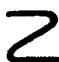
\includegraphics[keepaspectratio]{images/part001_587db9d1.jpg}}

\section{DIMENSION OF GRADED RINGS}

In this section, we denote by H a graded ring of type Z, with positive degrees, and by \((\mathrm{H}_{n})_{n\in\mathbf{Z}}\) its grading; thus we have \(H_{n}=\{0\}\) for n\textless0.

\subsection{Filtered ring associated with a graded ring}

For every \(n \in \mathbf{Z}\) , we set \(\mathrm{H}_{\geqslant n} = \sum_{i \geqslant n} \mathrm{H}_i\) . We have \(\mathrm{H} = \mathrm{H}_{\geqslant 0}\) ; the \(\mathrm{H}_{\geqslant n}\) are graded ideals of \(\mathrm{H}\) . Let S be the multiplicative subset \(1 + \mathrm{H}_{\geqslant 1}\) formed by the elements of H whose component of degree 0 is equal to 1, and consider the ring of fractions \(\mathrm{S}^{-1}\mathrm{H}\) . Identify H with a subring of its completion \(\hat{\mathrm{H}} = \prod_{n} \mathrm{H}_{n}\) (III, § 2, no. 12, example 1); since the elements of S are invertible in \(\hat{\mathrm{H}}\) (III, § 2, no. 13, lemma 3), \(\mathrm{S}^{-1}\mathrm{H}\) is identified with a subring of \(\hat{\mathrm{H}}\) containing H. For \(s \in \mathrm{S}\) and \(h \in \mathrm{H}_{\geqslant n}\) , the element \(s^{-1}h - h\) of \(\hat{\mathrm{H}}\) belongs to \(\prod_{i \geqslant n} \mathrm{H}_i\) ; consequently we have \(\mathrm{S}^{-1}\mathrm{H}_{\geqslant n} = (\mathrm{S}^{-1}\mathrm{H}) \cap \prod_{i \geqslant n} \mathrm{H}_i\) .

We deduce from this:

PROPOSITION 1. --- a) The ideals S \(^{-1}\) H \(_{≥n}\) form an exhaustive and separated filtration of the ring S \(^{-1}\) H.

\begin{enumerate}
\def\labelenumi{\alph{enumi})}
\setcounter{enumi}{1}
\tightlist
\item
  The canonical homomorphism from H to \(S^{-1}H\) induces for each n an isomorphism \(u_{n}\) of \(H_{n}\) onto \(S^{-1}H_{\geqslant n}/S^{-1}H_{\geqslant n+1}\) ; the \(u_{n}\) are the homogeneous components of an isomorphism of graded rings from H onto the graded ring associated with \(S^{-1}H\) , filtered by the \(S^{-1}H_{\geqslant n}\) .
\end{enumerate}

Remarks. --- 1) An element \(h/s\) of \(\mathrm{S}^{-1}\mathrm{H}\) with \(h\in\mathrm{H}, s\in\mathrm{S}\) , is invertible if and only if the component of degree 0 of \(h\) is invertible in \(\mathrm{H}_{0}\) . Consequently, if the ring \(\mathrm{H}_{0}\) is local, the ring \(\mathrm{S}^{-1}\mathrm{H}\) is local and the canonical injection \(\mathrm{H}_{0}\to\mathrm{S}^{-1}\mathrm{H}\) induces an isomorphism on the residue fields.

\begin{enumerate}
\def\labelenumi{\arabic{enumi})}
\setcounter{enumi}{1}
\tightlist
\item
  Suppose H is generated by \(H_{0}\) and \(H_{1}\) ; then for every n, we have \(H_{n+1} = H_{1}.H_{n}\) , hence \(H_{\geqslant n+1} = H_{1}.H_{\geqslant n}\) and \(S^{-1}H_{\geqslant n+1} = H_{1}.S^{-1}H_{\geqslant n}\) . Consequently, the filtration \((S^{-1}H_{\geqslant n})\) of \(S^{-1}H\) is the filtration \(S^{-1}H_{\geqslant 1}\) -adic.
\end{enumerate}

Examples. --- 1) * Let p be a graded prime ideal of C{[}X₀, \ldots, Xₙ{]} different from the ideal generated by the Xᵢ; let V be the algebraic subvariety of Pⁿ(C) defined by p and C the algebraic subvariety of Cⁿ⁺¹ defined by p. Then C is the cone over V, H = C{[}X₀, \ldots, Xₙ{]}/p is the affine algebra of C and S⁻¹H is the local ring of the cone C at its vertex. *

\begin{enumerate}
\def\labelenumi{\arabic{enumi})}
\setcounter{enumi}{1}
\tightlist
\item
  Let A be a local ring and a an ideal of A distinct from A. Then H = \(\bigoplus_{n} \mathfrak{a}^{n}/\mathfrak{a}^{n+1}\)
\end{enumerate}

is a graded ring such that \(H_{0} = A/\mathfrak{a}\) is local; it is generated by \(H_{0}\) and \(H_{1}\) . The ring \(S^{-1}H\) is therefore local and the filtration ( \(S^{-1}H_{\geq n}\) ) is the \(S^{-1}H_{\geq 1}\) -adic filtration. Note that in general the rings A and \(S^{-1}H\) are not isomorphic. * In particular, an algebraic variety is not in general locally isomorphic, in a neighborhood of a point, to its tangent cone at that point. *

\subsection{Dimension and chains of graded ideals}

In this issue, we will denote by dimgr(H) the supremum of the lengths of chains of graded prime ideals of H; likewise, if p is a graded prime ideal of H, we will denote by htgr(p) the supremum of the lengths of chains of graded prime ideals of H for which p is the largest element. If p is a graded prime ideal of H, we have \(p \cap S = \varnothing\); otherwise, indeed p would contain an element whose degree-0 component equals 1, hence would contain 1 since it is graded. The map \(p \mapsto S^{-1}p\) from the set of graded prime ideals of H to the set of prime ideals of \(S^{-1}H\) is therefore injective and increasing (II, § 2, no. 5, prop. 11); consequently, in view of § 1, no. 3, prop. 6 and the corollary to prop. 7, we have:

PROPOSITION 2. --- a) We have \(\dim \mathrm{gr}(\mathrm{H}) \leqslant \dim (\mathrm{S}^{-1}\mathrm{H}) \leqslant \dim (\mathrm{H})\) .

\begin{enumerate}
\def\labelenumi{\alph{enumi})}
\setcounter{enumi}{1}
\tightlist
\item
  For every graded prime ideal \(\mathfrak{p}\) from H, we have \(\operatorname{htgr}(\mathfrak{p}) \leqslant \operatorname{ht}(\mathrm{S}^{-1}\mathfrak{p}) = \operatorname{ht}(\mathfrak{p})\) .
\end{enumerate}

For every ideal a of H, denote \(a^{gr}\) the largest graded ideal contained in a; we have \(a^{gr} = \sum_{n} (a \cap H_n)\) .

Lemma 1. --- a) If p is a prime ideal of H, \(\mathfrak{p}^{\mathrm{gr}}\) is a prime ideal.

\begin{enumerate}
\def\labelenumi{\alph{enumi})}
\setcounter{enumi}{1}
\item
  Every maximal element of the set of graded ideals of H distinct from H is a maximal ideal of H that contains \(H_{\geq1}\) .
\item
  Every minimal prime ideal of H is graded.
\item
  This follows from III, § 1, no. 4, prop. 4.
\item
  Let m be a graded ideal of H distinct from H. Then we have
\end{enumerate}

\[
\mathfrak {m} \subset (\mathfrak {m} \cap \mathrm{H} _ {0}) + \mathrm{H} _ {\geqslant 1} \neq \mathrm{H}.
\]

If m is maximal, then we have \(m = m_{0} + H_{\geq 1}\) , where \(m_{0}\) is a maximal ideal of \(H_{0}\) , whence b).

\begin{enumerate}
\def\labelenumi{\alph{enumi})}
\setcounter{enumi}{2}
\tightlist
\item
  Let p be a minimal prime ideal of H. Since \(p^{gr}\) is prime by a) and contained in p, we have \(p = p^{gr}\) whence c).
\end{enumerate}

Lemma 2.---Let p and q be prime ideals of H such that q ⊂ p and q ≠ p. If q \(^{gr}\) = p \(^{gr}\) then q is graded, p is not, and ht(p/q) = 1.

Remark 1.--- Let us take up the notations of example 1 of no. 1. Lemma 2 implies that, if two irreducible subvarieties Y and Z of \(\mathbf{C}^{n+1}\) have the same projecting cone and if \(Z \subset Y\) and \(Z \neq Y\) , then Y is the projecting cone of Z, and Z has codimension 1 in Y. *

Replacing H by \(\mathrm{H} / \mathfrak{q}^{\mathrm{gr}}\) we reduce to the case where \(\mathfrak{q}^{\mathrm{gr}} = \{0\}\). Then H is integral (lemma 1, a)), \(\mathfrak{p}^{\mathrm{gr}} = 0\) , and the task is to prove that \(\operatorname{ht}(\mathfrak{p}) \leqslant 1: this will indeed imply that  \operatorname{ht}(\mathfrak{q}) = 0\) , hence that \(\mathfrak{q} = \{0\}\) . Since \(\mathfrak{p}^{\mathrm{gr}} = \{0\}\) , one has \(\mathfrak{p} \cap \mathrm{H}_n = \{0\}\) for every \(n\) , and \(\mathfrak{p}\) is disjoint from the multiplicative subset \(\mathrm{T} = \bigcup_{n} (\mathrm{H}_n - \{0\})\) . The ring \(\mathrm{H}_{\mathfrak{p}}\) is therefore isomorphic to a ring of fractions of \(\mathrm{T}^{-1}\mathrm{H}\) , and we therefore have

\[
\mathrm{ht} (\mathfrak {p}) = \dim (\mathrm{H} _ {\mathfrak {p}}) \leqslant \dim (\mathrm{T} ^ {- 1} \mathrm{H})
\]

(§ 1, no. 3, props. 6 and 7). But, by Lemma 4 of V, § 1, no. 8, T \(^{-1}\) H is a field or is isomorphic to a ring K{[}X, X \(^{-1}\) {]}, where K is a field; we therefore have dim(T \(^{-1}\) H) ≤ 1 and ht(p) ≤ 1, which is what we wanted to prove.

PROPOSITION 3. --- Let p be a prime ideal of H. If p ≠ p \(^{gr}\) , we have ht(p \(^{gr}\) ) = ht(p) - 1. By Lemma 1, a), the ideal p \(^{gr}\) is prime and contained in p, hence ht(p \(^{gr}\) ) ≤ ht(p) - 1. The proposition being trivial when ht(p \(^{gr}\) ) = +∞, we may assume ht(p \(^{gr}\) ) \textless{} + ∞. Let us prove the inequality ht(p) ≤ ht(p \(^{gr}\) ) + 1 by induction on ht(p \(^{gr}\) ). It suffices to prove that, for every prime ideal q contained in p and distinct from p, one has ht(q) ≤ ht(p \(^{gr}\) ). We distinguish two cases according as q \(^{gr}\) ≠ p \(^{gr}\) or that q \(^{gr}\) = p \(^{gr}\) . If q \(^{gr}\) ≠ p \(^{gr}\) , then we have ht(q \(^{gr}\) ) \textless{} ht(p \(^{gr}\) ); we have

\[
\mathrm{ht} (\mathfrak {q}) \leqslant \mathrm{ht} (\mathfrak {q} ^ {\mathrm{gr}}) + 1,
\]

by the induction hypothesis if q ≠ q \(^{gr}\) and trivially if q = q \(^{gr}\) ; consequently, we have ht(q) ≤ ht(q \(^{gr}\) ) + 1 ≤ ht(p \(^{gr}\) ), which is what we wanted to prove. If q \(^{gr}\) = p \(^{gr}\) , then we have q = q \(^{gr}\) by Lemma 2, hence ht(q) = ht(q \(^{gr}\) ) ≤ ht(p \(^{gr}\) ), whence again the desired conclusion.

THEOREM 1. --- Assume H is Noetherian.

\begin{enumerate}
\def\labelenumi{\alph{enumi})}
\item
  Every chain of graded prime ideals of H, saturated as a chain of graded prime ideals, is saturated as a chain of prime ideals.
\item
  For every graded prime ideal p of H, one has htgr(p) = ht(S \(^{-1}\) p) = ht(p).
\item
  We have \(\dim \mathrm{gr}(\mathbf{H}) = \dim (\mathbf{S}^{-1}\mathbf{H}) = \dim (\mathbf{H}).\)
\end{enumerate}

To prove \(a\) ), it suffices to show that, if \(\mathfrak{p}\) and \(\mathfrak{q}\) are two distinct graded prime ideals of H such that \(\mathfrak{q} \subset \mathfrak{p}\) and every graded prime ideal between \(\mathfrak{q}\) and \(\mathfrak{p}\) is equal to \(\mathfrak{p}\) or to \(\mathfrak{q}\) , then \(\mathrm{ht}(\mathfrak{p}/\mathfrak{q}) = 1\) . By dividing by \(\mathfrak{q}\) , one reduces to the case where \(\mathfrak{q} = \{0\}\) . It therefore remains to prove that, if H is integral, and if \(\mathfrak{p}\) is an ideal of H, minimal among the graded prime ideals \(\neq \{0\}\) , one has \(\mathrm{ht}(\mathfrak{p}) = 1\) . Now let \(a\) be a nonzero homogeneous element of \(\mathfrak{p}\) , and let r be a prime ideal of H such that \(a \in \mathfrak{r} \subset \mathfrak{p}\) and minimal for these properties (II, § 2, no. 6, lemma 2). Since \(\mathfrak{r}^{\mathrm{gr}}\) is prime (lemma 1, \(a\) ) and nonzero, we have \(\mathfrak{r}^{\mathrm{gr}} = \mathfrak{p}\) , hence \(\mathfrak{p} = \mathfrak{r}\) . Since H is integral and Noetherian, \(\mathfrak{p}\) has height 1 (§ 3, no. 1, prop. 1), whence \(a\) ).

Let us prove b). Let p be a graded prime ideal of H. We have

\[
\operatorname{htgr} (\mathfrak {p}) \leqslant \operatorname{ht} \left(\mathrm{S} ^ {- 1} \mathfrak {p}\right) \leqslant \operatorname{ht} (\mathfrak {p})
\]

(prop. 2); let us prove the inequality ht(p) ≤ htgr(p) by induction on htgr(p). If htgr(p) = 0, p is minimal among graded prime ideals, hence minimal (lemma 1, c)), and we have ht(p) = 0. Suppose that htgr(p) \textgreater{} 0 and let us prove the inequality ht(q) ≤ htgr(p) - 1 for every prime ideal q contained in p and distinct from p. Let us distinguish two cases. If q is graded, we conclude by the induction hypothesis. If q is not graded, then we have q \(^{gr}\) ≠ p, hence ht(q \(^{gr}\) ) ≤ htgr(q \(^{gr}\) ) by the induction hypothesis, whence ht(q) ≤ htgr(q \(^{gr}\) ) + 1 by prop. 3; it remains to prove the inequality htgr(q \(^{gr}\) ) ≤ htgr(p) - 2; but if we had htgr(q \(^{gr}\) ) = htgr(p) - 1, the chain q \(^{gr}\) ⊂ p would be saturated by a), which is not the case since q \(^{gr}\) ≠ q ≠ p.

Let us finally prove c). We have dimgr(H) ≤ dim(S⁻¹H) ≤ dim(H) (prop. 2), and it remains to prove dim(H) ≤ dimgr(H), or equivalently ht(p) ≤ dimgr(H) for every prime ideal p of H. Let p therefore be a prime ideal of H. If p is graded, we have ht(p) = htgr(p) ≤ dimgr(H). If p is not graded, we have ht(p) = htgr(p\(^{\mathrm{gr}}\)) + 1 by prop. 3; let m be a maximal graded ideal of H containing p\(^{\mathrm{gr}}\); by lemma 1, b), m is maximal, hence distinct from p\(^{\mathrm{gr}}\), and we have htgr(p\(^{\mathrm{gr}}\)) + 1 ≤ htgr(m) ≤ dimgr(H), whence again ht(p) ≤ dimgr(H). This completes the proof.

Remark 2. --- There exist non-Noetherian graded rings H such that dimgr(H) \textless{} dim(H) (p.~99, exercise 1).

\subsection{Dimension of graded modules}

In this number, we denote by M a graded H-module (of type Z).

Then \(\mathbf{S}^{-1}\mathbf{M}\) is an \(\mathbf{S}^{-1}\mathbf{H}\)-module, and if we set \(\mathbf{M}_{\geqslant n} = \bigoplus_{i\geqslant n}\mathbf{M}_i\) , we see as in

no. 1 that the sequence of sets \(S^{-1}M_{\geqslant n}\) is an exhaustive and separated filtration on

\(S^{-1}M\) and that the canonical map \(M \to S^{-1}M\) induces an isomorphism from M onto the graded module \(\oplus S^{-1}M_{\geqslant n}/S^{-1}M_{\geqslant n+1}\) .

Lemma 3. --- Suppose H is generated by \(\mathbf{H}_{0} \cup \mathbf{H}_{1}\) and M generated by \(\bigoplus_{i \leqslant n_{0}} \mathbf{M}_{i}\) for a suitable integer \(n_{0}\). Then the filtration \((\mathbf{S}^{-1}\mathbf{M}_{\geqslant n})\) of \(\mathbf{S}^{-1}\mathbf{M}\) is good for the ideal \(\mathbf{S}^{-1}\mathbf{H}_{\geqslant 1}\) of \(\mathbf{S}^{-1}\mathbf{H}\) .

We have, for \(n \geqslant n_0\) , \(\mathbf{M}_{\geqslant n+1} = \mathbf{H}_1 \cdot \mathbf{M}_{\geqslant n}\) , hence \(\mathbf{S}^{-1} \mathbf{M}_{\geqslant n+1} = \mathbf{H}_1 \cdot \mathbf{S}^{-1} \mathbf{M}_{\geqslant n} = \mathbf{S}^{-1} \mathbf{H}_{\geqslant 1} \cdot \mathbf{S}^{-1} \mathbf{M}_{\geqslant n}\) .

PROPOSITION 4. --- Suppose H is Noetherian and M is finitely generated. Then \(\dim_{\mathbf{H}}(\mathbf{M}) = \dim_{\mathbf{S}^{-1}\mathbf{H}}(\mathbf{S}^{-1}\mathbf{M})\) .

Let a be the annihilator of the H-module M; it is a graded ideal of H. Since M is a finitely generated H-module, the annihilator of the S \(^{-1}\) H-module S \(^{-1}\) M is the ideal S \(^{-1}\) a of S \(^{-1}\) H. We have dim \(_{H}\) (M) = dim(H/a) and dim \(_{S^{-1}H}\) (S \(^{-1}\) M) = dim(S \(^{-1}\) H/S \(^{-1}\) a). Prop. 4 then follows from th. 1, c) of no. 2 applied to the graded ring H/a.

Proposition 5. — Suppose \(\mathbf{H}_{0}\) is local and Artinian, \(\mathbf{H}\) is generated by \(\mathbf{H}_{0} \cup \mathbf{H}_{1}\) , \(\mathbf{H}_{1}\) is of finite type as a \(\mathbf{H}_{0}\) -module, and \(\mathbf{M}\) is nonzero and of finite type as an \(\mathbf{H}\) -module. Then \(\mathbf{M}_{n}\) is a nonzero finitely generated \(\mathbf{H}_{0}\) -module of finite length for each \(n\) , and there exists \(\mathbf{Q}(\mathbf{T}) \in \mathbf{Z}[\mathbf{T}, \mathbf{T}^{-1}]\) such that \(\mathbf{Q}(1) > 0\) and that one has in the ring \(\mathbf{Z}((\mathbf{T}))\)

\[
\sum_ {n \in \mathbf {Z}} \mathrm{long} _ {\mathrm{H} _ {0}} (\mathrm{M} _ {n}). \mathrm{T} ^ {n} = (1 - \mathrm{T}) ^ {- d}. \mathrm{Q} (\mathrm{T}),
\]

with \(d = \dim_{\mathbf{H}}(\mathbf{M})\).

The ring \(\mathbf{S}^{-1}\mathbf{H}\) is local and Noetherian (no. 1, remark 1), the \(\mathbf{S}^{-1}\mathbf{H}\) -module \(\mathbf{S}^{-1}\mathbf{M}\) is nonzero of finite type, and of dimension \(d = \dim_{\mathbf{H}}(\mathbf{M})\) (prop. 4). Moreover, \(\mathbf{S}^{-1}\mathbf{H}_{\geqslant 1}\) is a defining ideal of \(\mathbf{S}^{-1}\mathbf{H}\) (§ 3, no. 2, Lemma 2) and \(\mathbf{S}^{-1}\mathbf{M}_{\geqslant n}\) is a filtration \(\mathbf{S}^{-1}\mathbf{H}_{\geqslant 1}\) -good on \(\mathbf{S}^{-1}\mathbf{M}\) (Lemma 3). Finally, we have long \(_{\mathbf{S}^{-1}\mathbf{H}}\mathbf{S}^{-1}\mathbf{M}_{\geqslant n}/\mathbf{S}^{-1}\mathbf{M}_{\geqslant n+1} = \text{long}_{\mathbf{H}_0}(\mathbf{M}_n)\) for every \(n\). It therefore suffices to apply theorems 2 and 3 of § 4 (nos. 3 and 4).

Remark. --- Except for the determination of the integer d, prop. 5 follows directly from th. 1 of § 4, no. 2.

COROLLARY. --- Let A be a Noetherian local ring and q an ideal of definition of A. Then we have \(\dim(A) = \dim(\text{gr}_{\mathfrak{q}}(A))\) .

Applying prop. 5 to the case M = H = gr\_q(A), we obtain the relation

\[
\sum_ {n \geqslant 0} \mathrm{long} _ {\mathrm{A} / \mathfrak {q}} (\mathfrak {q} ^ {n} / \mathfrak {q} ^ {n + 1}). \mathrm{T} ^ {n} = (1 - \mathrm{T}) ^ {- d} \mathrm{Q} (\mathrm{T})
\]

with \(d = \dim(\mathrm{gr}_{\mathfrak{q}}(\mathbf{A}))\) and \(\mathbf{Q}(1) \neq 0\) . We have \(d = \dim(\mathbf{A})\) by th. 3 of § 4, no. 4, whence the corollary.

PROPOSITION 6. --- Suppose \(\mathbf{H}_{0}\) is local and Artinian, \(\mathbf{H}\) is of finite type as a \(\mathbf{H}_{0}\) -algebra and \(\mathbf{M}\) is of finite type as a \(\mathbf{H}\) -module.

\begin{enumerate}
\def\labelenumi{\alph{enumi})}
\item
  Let \(a_1, \ldots, a_n\) be elements of H, homogeneous of degrees \(> 0\) , and let \(\varphi\) be the homomorphism (of \(\mathbf{H}_0\) -algebras) from \(\mathbf{H}_0[\mathbf{X}_1, \ldots, \mathbf{X}_n]\) to H which sends \(\mathbf{X}_i\) to \(a_i\) for \(1 \leqslant i \leqslant n\) . The \(S^{-1}H\) -module \(S^{-1}M / \sum_{i=1}^{n}(a_i/1) \cdot S^{-1}M\) is of finite length if and only if \(\varphi_*(M)\) is a finitely generated module over \(\mathbf{H}_0[\mathbf{X}_1, \ldots, \mathbf{X}_n]\) .
\item
  There exists a family \((a_{1},...,a_{d})\) of elements of H, all homogeneous of the same degree \textgreater0, with \(d=\dim_{\mathrm{H}}(\mathbf{M})\) and such that \((a_{1}/1,...,a_{d}/1)\) is a maximal secant sequence for the \(S^{-1}H\) -module \(S^{-1}M\) . If moreover H is generated by \(H_{1}\) as \(H_{0}\) -algebra, and if the residue field of \(H_{0}\) is infinite, one may take the \(a_{i}\) of degree 1.
\item
  Set \(\mathbf{N} = \mathbf{M} / \sum_{i=1}^{n} a_i \mathbf{M}\) . We have \(\dim_{\mathrm{H}}(\mathbf{N}) = \dim_{\mathrm{S}^{-1}\mathrm{H}}(\mathrm{S}^{-1}\mathrm{N})\) by prop. 4. Consequently, the \(\mathrm{S}^{-1}\mathrm{H}\) -module \(\mathrm{S}^{-1}\mathrm{N}\) is of finite length if and only if the H-module N is of finite length, that is, if and only if N is a \(\mathrm{H}_0\) -module of finite type. If \(\varphi_*(\mathbf{M})\) is the module over \(\mathrm{H}_0[\mathrm{X}_1, ..., \mathrm{X}_n]\) deduced from M by the homomorphism \(\varphi : \mathrm{H}_0[\mathrm{X}_1, ..., \mathrm{X}_n] \to \mathbf{H}\) , one has \(\mathbf{N} = \varphi_*(\mathbf{M}) / \sum_{i=1}^{n} X_i \cdot \varphi_*(\mathbf{M})\) . Consequently (A, II, p.~171, cor. 3 and remark) \(\varphi_*(\mathbf{M})\) is a finitely generated module over \(\mathrm{H}_0[\mathrm{X}_1, ..., \mathrm{X}_n]\) if and only if N is a \(\mathrm{H}_0\) -module of finite type. This proves a).
\end{enumerate}

To prove b), we will first establish a lemma.

Lemma 4. --- Let \(b\) be an element of H, homogeneous of degree \(>0\), and not belonging to any of the minimal elements \(\mathfrak{p}\) of \(\operatorname{Supp}(\mathbf{M})\) such that \(\dim(\mathrm{H}/\mathfrak{p}) = \dim_{\mathrm{H}}(\mathbf{M})\). We then have \(\dim_{\mathrm{H}}(\mathbf{M}/b\mathbf{M}) = \dim_{\mathrm{H}}(\mathbf{M}) - 1\).

Set \(d = \dim_{\mathbf{H}}(\mathbf{M})\). By the definition of \(b\) , one has \(\dim_{\mathbf{H}}(\mathbf{M}/b\mathbf{M}) < d\). By prop. 4, we have

\[
\dim_ {\mathrm{H}} (\mathrm{M} / b \mathrm{M}) = \dim_ {\mathrm{S} ^ {- 1} \mathrm{H}} \left(\mathrm{S} ^ {- 1} \mathrm{M} / (b / 1). \mathrm{S} ^ {- 1} \mathrm{M}\right)
\]

and formula (8) of § 3, no. 2 yields the inequality

\[
\dim_ {\mathrm{S} ^ {- 1} \mathrm{H}} (\mathrm{S} ^ {- 1} \mathrm{M} / (b / 1). \mathrm{S} ^ {- 1} \mathrm{M}) \geqslant \dim_ {\mathrm{S} ^ {- 1} \mathrm{H}} (\mathrm{S} ^ {- 1} \mathrm{M}) - 1.
\]

Finally, we have

\[
\dim_ {S ^ {- 1} H} (S ^ {- 1} M) = \dim_ {H} (M) = d
\]

by prop. 4. We therefore have \(\dim_{\mathrm{H}}(\mathrm{M}/b\mathrm{M}) \geqslant d - 1\) , whence lemma 4.

Let us resume the proof of prop. 6, b). We may assume \(\dim_{\mathbf{H}}(\mathbf{M}) > 0\). Note that every minimal element of \(\operatorname{Supp}(\mathbf{M})\) is graded (apply Lemma 1 of No. 2 to the quotient of H by the annihilator of M). By Prop. 8 of III, § 1, No. 4, there therefore exists a homogeneous element \(b\) of H, of degree \(>0\), not belonging to any of the minimal elements \(\mathfrak{p}\) of \(\operatorname{Supp}(\mathbf{M})\) such that \(\dim(\mathrm{H}/\mathfrak{p}) = \dim_{\mathbf{H}}(\mathbf{M})\). By Lemma 4, we have \(\dim_{\mathbf{H}}(\mathbf{M}/b\mathbf{M}) = \dim_{\mathbf{H}}(\mathbf{M}) - 1\). Suppose moreover that H is generated by \(\mathrm{H}_{1}\) as \(\mathrm{H}_{0}\) -algebra and the residue field \(k\) of \(\mathrm{H}_{0}\) is infinite. For every minimal element \(\mathfrak{p}\) of \(\operatorname{Supp}(\mathbf{M})\) such that \(\dim(\mathrm{H}/\mathfrak{p}) = \dim_{\mathbf{H}}(\mathbf{M})\) , consider the vector subspace \(\mathrm{V}_{\mathfrak{p}} = (\mathfrak{p} \cap \mathrm{H}_{1}) \otimes_{\mathrm{H}_{0}} k\) of the \(k\)-vector space \(\mathrm{V} = \mathrm{H}_{1} \otimes_{\mathrm{H}_{0}} k\). If one had \(\mathrm{V}_{\mathfrak{p}} = \mathrm{V}\) , one would have \(\mathfrak{p} \cap \mathrm{H}_1 = \mathrm{H}_1\) (II, §3, no. 2, prop. 4), whence \(\mathrm{H}_1 \subset \mathfrak{p}\) and \(\dim_{\mathrm{H}}(\mathbf{M}) = \dim(\mathrm{H}/\mathfrak{p}) \leqslant \dim(\mathrm{H}/\mathrm{H}_{\geqslant 1}) = 0\) , which is not the case. Since \(k\) is assumed to be infinite, the union of the \(\mathrm{V}_{\mathfrak{p}}\) is distinct from V; if \(b \in \mathrm{H}_1\) is such that \(b \otimes 1\) belongs to none of the \(\mathrm{V}_{\mathfrak{p}}\) , one has \(\dim(\mathrm{M}/b\mathrm{M}) = \dim_{\mathrm{H}}(\mathrm{M}) - 1\) .

Proceeding by induction on \(d = \dim_{\mathbf{H}}(\mathbf{M})\) , one then constructs a sequence \((b_1, \ldots, b_d)\) of elements of H, with \(b_i\) homogeneous of degree \(n_i > 0\) and such that \(\mathbf{M} / \sum_{i=1}^{n} b_i \mathbf{M}\) is an H-module of finite length. If one assumes H is generated by \(\mathbf{H}_1\) as \(\mathbf{H}_0\) -algebra and the residue field of \(\mathbf{H}_0\) infinite, one may assume \(n_i = 1\) for \(i = 1, \ldots, d\). By prop. 4, we have \(\dim_{\mathbf{S}^{-1}\mathbf{H}}(\mathbf{S}^{-1}\mathbf{M}) = d\) and

\[
\dim_ {\mathrm{S} ^ {- 1} \mathrm{H}} (\mathrm{S} ^ {- 1} \mathrm{M} / \sum_ {i = 1} ^ {d} (b _ {i} / 1). \mathrm{S} ^ {- 1} \mathrm{M}) = 0.
\]

Then \((b_{1} / 1,\dots,b_{d} / 1)\) is a maximal secant sequence for the \(\mathbf{S}^{-1}\mathbf{H}\) -module \(\mathbf{S}^{-1}\mathbf{M}\) . Put \(a_{i} = b_{i}^{(n_{1}\dots n_{d}) / n_{i}}\) for \(1\leqslant i\leqslant d\) ; then the \(a_{i}\) are all of the same degree, and \((a_{1} / 1,\dots,a_{d} / 1)\) is a maximal secant sequence for \(\mathbf{S}^{-1}\mathbf{M}\) (§ 3, no. 2, Remark 3).

COROLLARY 1. --- Suppose that \(\mathbf{H}_0\) is a field and that \(\mathbf{H}\) is of finite type as an \(\mathbf{H}_0\) -algebra. Set \(n = \dim(\mathbf{H})\) . There exist homogeneous elements \(a_1, ..., a_n\) of \(\mathbf{H}\) all of the same degree \(>0\) , such that the \(\mathbf{H}_0\) -homomorphism \(\varphi: \mathbf{H}_0[\mathbf{X}_1, ..., \mathbf{X}_n] \to \mathbf{H}\) defined by \(\varphi(\mathbf{X}_i) = a_i\) , \(i = 1, ..., n\) , be injective and make \(\mathbf{H}\) a finite \(\mathbf{H}_0[\mathbf{X}_1, ..., \mathbf{X}_n]\)-algebra. If \(\mathbf{H}\) is generated by \(\mathbf{H}_1\) as \(\mathbf{H}_0\) -algebra and if \(\mathbf{H}_0\) is infinite, one may assume the \(a_i\) of degree 1.

There exists, by prop. 6, a \(\mathbf{H}_0\) -homomorphism \(\varphi\) of the indicated form that makes H a \(\mathbf{H}_0[\mathbf{X}_1, \ldots, \mathbf{X}_n]\) -finite algebra. By th. 1 of § 2, no. 3, we then have

\[
\dim \left(\mathrm{H} _ {0} \left[ \mathrm{X} _ {1}, \dots , \mathrm{X} _ {n} \right] / (\operatorname{Ker} \varphi)\right) = \dim (\mathrm{H});
\]

since we have

\[
\dim (\mathrm{H}) = n = \dim \left(\mathrm{H} _ {0} \left[ \mathrm{X} _ {1}, \dots , \mathrm{X} _ {n} \right]\right),
\]

and that \(\mathrm{H}_0[\mathrm{X}_1, \dots, \mathrm{X}_n]\) is an integral domain, this implies \(\operatorname{Ker} \varphi = \{0\}\) .

Note. --- Let \((h_{1}, \ldots, h_{r})\) be a finite generating system of the \(H_{0}\) -vector space \(H_{1}\) . For \(\lambda = (\lambda_{1}, \ldots, \lambda_{r}) \in H_{0}^{r}\) , set \(h_{\lambda} = \lambda_{1} h_{1} + \cdots + \lambda_{r} h_{r}\). The proofs of Prop. 6 and Cor. 1 yield the following result: the set of elements \((\lambda_{1}, \ldots, \lambda_{n})\) of \((\mathrm{H}_{0}^{r})^{n}\) such that the elements \(a_{i} = h_{\lambda_{i}} \in H_{1}\) satisfy the conclusion of Cor. 1, contains the complement of the union of a finite number of vector subspaces of \((\mathrm{H}_{0}^{r})^{n}\) distinct from the entire space.

COROLLARY 2. --- Let A be a Noetherian local ring and \(n\in\mathbb{N}\). For one to have \(\dim(\mathbf{A})\geqslant n\) it is necessary and sufficient that for every integer \(r\geqslant0\) , one has

\[
\left[ \mathfrak {m} _ {\mathrm{A}} ^ {r} / \mathfrak {m} _ {\mathrm{A}} ^ {r + 1}: \kappa_ {\mathrm{A}} \right] \geqslant \binom {n + r - 1} {n - 1}, \quad \left(\text { resp.   long } _ {\mathrm{A}} (\mathrm{A} / \mathfrak {m} _ {\mathrm{A}} ^ {r + 1}) \geqslant \binom {n + r} {n}\right);
\]

We have equality for every r if and only if A is regular of dimension n.

The condition is sufficient (§ 4, no. 4, th. 3 and § 5, no. 2, th. 1). Let us show that it is necessary. Consider the graded ring gr(A) = gr \(_{m_A}\) (A); let k be an infinite extension of the field κ \(_A\) , and set H = k ⊗ κ \(_A\) gr(A). The ring H has dimension ≥ n (prop. 5 and its corollary); hence, from cor. 1, we deduce the existence of an injective graded homomorphism of graded k-algebras φ : H \(_0\) {[}X \(_1\) , \ldots, X \(_n\) {]} → H. Consequently, for every integer r ≥ 0,

\[
\left[ \mathrm{gr} _ {r} (\mathrm{A}): \kappa_ {\mathrm{A}} \right] = \left[ \mathrm{H} _ {r}: \mathrm{H} _ {0} \right] \geqslant \binom {n + r - 1} {n - 1},
\]

and the equality for every \(r\) implies the bijectivity of \(\varphi\) , hence the regularity of A ( \(\S\) 5, no. 2, th. 1).

The equalities

\[
\mathrm{long} _ {\mathbf {A}} (\mathrm{A} / \mathfrak {m} _ {\mathbf {A}} ^ {r + 1}) = \sum_ {i = 0} ^ {r} \left[ \mathrm{gr} _ {i} (\mathbf {A}): \kappa_ {\mathbf {A}} \right]
\]

and

\[
\binom {n + r} {n} = \sum_ {i = 0} ^ {r} \binom {n + i - 1} {n - 1}
\]

then imply the analogous assertions for the function \(r \mapsto \text{long}_{\mathbf{A}}(\mathbf{A}/m_{\mathbf{A}}^{r+1})\) .

\subsection{Semicontinuity of dimension}

Lemma 5.--- Let A be a ring, r its radical, \(\mathbf{R} = \bigoplus_{i \in \mathbf{Z}} \mathbf{R}_i\) a graded A-algebra, \(\mathbf{M} = \bigoplus_{i \in \mathbf{Z}} \mathbf{M}_i\) a graded R-module. We assume that each \(\mathbf{M}_i\) is an A-module of finite type

and that M/rM is a finitely generated R/rR-module. Then M is a finitely generated R-module. Let \(m_{1}, \ldots, m_{n}\) be homogeneous elements of M, whose images in M/rM generate the R/rR-module M/rM. Let N be the (graded) sub-R-module of M generated by \(\{m_{1}, \ldots, m_{n}\}\) . For every \(i \in \mathbf{Z}\) , one has \(M_{i} = N_{i} + rM_{i}\) , hence \(M_{i} = N_{i}\) (II, §3, no. 2, prop. 4); consequently, we have M = N.

Lemma 6. --- Let \(\rho: \mathbf{B} \to \mathbf{C}\) be a ring homomorphism and S a multiplicative subset of B. Suppose that C is a finitely generated B-algebra, and that \(\mathbf{S}^{-1}\mathbf{C}\) is a finite \(\mathbf{S}^{-1}\mathbf{B}\)-algebra. There then exists \(f \in \mathbf{S}\) such that \(\mathbf{C}_f\) is a finite \(\mathbf{B}_f\)-algebra.

Let X be a finite generating set of the B-algebra C. For every \(x \in X\), the image of x in \(S^{-1}C\) is integral over \(S^{-1}B\), and there consequently exist an integer \(n(x) \geqslant 0\), elements \(b_{1}(x), \ldots, b_{n(x)}(x) \in B\), and an element \(f(x) \in S\) such that

\[
f (x) x ^ {n (x)} + b _ {1} (x) x ^ {n (x) - 1} + \dots + b _ {n (x)} = 0.
\]

Let \(f = \prod_{x \in X} f(x)\) ; the image of every element \(x\) of \(X\) in \(C_f\) is integral over \(B_f\) , hence \(C_f\) is a finite \(B_f\)-algebra (V, § 1, no. 1, prop. 4).

PROPOSITION 7. — Suppose that H is an \(H_{0}\)-algebra of finite type. Then the function \(\mathfrak{p} \mapsto \dim(\mathrm{H} \otimes_{\mathrm{H}_{0}} \kappa(\mathfrak{p}))\) is upper semicontinuous on \(\operatorname{Spec}(\mathrm{H}_{0})\) .

Since H is finitely generated as an \(H_{0}\)-algebra, each \(H_{i}\) is a finitely generated \(H_{0}\)-module (III, § 1, no. 2, corollary to prop. 1), and H is generated as an \(H_{0}\)-algebra by \(H_{0} \oplus H_{1} \oplus \cdots \oplus H_{r}\) for a suitable integer \(r \geqslant 0\). Let \(\mathfrak{p} \in \operatorname{Spec}(H_{0})\) and set \(\dim(H \otimes_{H_{0}} \kappa(\mathfrak{p})) = n \geqslant 0\). By Corollary 1 to Prop. 6, there exist elements \(a_{1}, ..., a_{n}\) of H, all homogeneous of the same degree \(d > 0\), such that the \(\kappa(\mathfrak{p})\)-homomorphism \(\overline{\varphi}: \kappa(\mathfrak{p})[X_{1}, ..., X_{n}] \to H \otimes_{H_{0}} \kappa(\mathfrak{p})\) which maps \(X_{i}\) to \(a_{i} \otimes 1\) for \(1 \leqslant i \leqslant n\), makes \(H \otimes_{H_{0}} \kappa(\mathfrak{p})\) a finite \(\kappa(\mathfrak{p})[X_{1}, ..., X_{n}]\)-algebra. Let \(\varphi\) be the \(H_{0}\)-homomorphism from \(H_{0}[X_{1}, ..., X_{n}] = R\) to H which maps \(X_{i}\) to \(a_{i}\) for \(1 \leqslant i \leqslant n\). If one sets, for every \(m \in \mathbf{Z}\), \(H_{m}' = \sum_{(m-1)d < i \leqslant md} H_{i}\), one obtains a grading of type \(\mathbf{Z}\) on H, compatible with the R-module structure given by \(\varphi\). Each \(H_{m}'\) is of finite type over \(H_{0}\). By Lemma 5, \(H_{\mathfrak{p}}\) is a finitely generated \(R_{\mathfrak{p}}\)-module. By Lemma 6, there therefore exists \(f \in H_{0} - \mathfrak{p}\) such that \(H_{f}\) is an \(R_{f}\)-module of finite type. For every \(\mathfrak{q} \in \operatorname{Spec}(H_{0})_{f}\), \(H \otimes_{H_{0}} \kappa(\mathfrak{q})\) is a finite \(\kappa(\mathfrak{q})[X_{1}, ..., X_{n}]\)-algebra, hence \(\dim(H \otimes_{H_{0}} \kappa(\mathfrak{q})) \leqslant n\) (\S 2, n° 3, th. 1), which completes the proof.

Remarks. --- 1) * In algebraic geometry, prop. 7 implies that the dimension of the fibers of a projective morphism of algebraic varieties is upper semi-continuous. *

\begin{enumerate}
\def\labelenumi{\arabic{enumi})}
\setcounter{enumi}{1}
\tightlist
\item
  We will see later that if \(\rho:A\to B\) is a ring homomorphism that makes \(B\) a \(A\) -algebra of finite type, the function \(\mathfrak{q}\mapsto\dim_{\mathfrak{q}}(B\otimes_{A}\kappa(\rho^{-1}(q)))\) is upper semicontinuous on \(\operatorname{Spec}(B)\) (cf. p. 101, exerc. 10).
\end{enumerate}

\subsection{Graded regular algebras}

In this issue, we assume that \(H_{0}\) is a field and that H is an \(H_{0}\)-algebra of finite type.

One sets \(H_{+} = H_{\geqslant 1}\) ; it is a maximal ideal of H. The ring \(S^{-1}H\) is identified with the local ring \(H_{H_{+}}\) of H at the ideal \(H_{+}\) ; its maximal ideal is \((\mathrm{H}_{+})_{\mathrm{H}_{+}} = \mathrm{S}^{-1}\mathrm{H}_{+}\) , its residue field is identified with \(H_{0}\) .

PROPOSITION 8. --- a) We have \(\dim(\mathbf{H}) \leqslant [\mathbf{H}_{+}/\mathbf{H}_{+}^{2}:\mathbf{H}_{0}]\) .

\begin{enumerate}
\def\labelenumi{\alph{enumi})}
\setcounter{enumi}{1}
\tightlist
\item
  The following conditions are equivalent:
\end{enumerate}

\begin{enumerate}
\def\labelenumi{(\roman{enumi})}
\item
  \(\dim (\mathrm{H}) = [\mathrm{H}_{+} / \mathrm{H}_{+}^{2}:\mathrm{H}_{0}]\) ;
\item
  the Noetherian local ring \(\mathbf{S}^{-1}\mathbf{H}\) is regular ;
\item
  H is generated as \(H_{0}\) -algebra by a family of homogeneous elements of degrees \textgreater{} 0, algebraically independent over \(H_{0}\) .
\end{enumerate}

\begin{enumerate}
\def\labelenumi{\alph{enumi})}
\setcounter{enumi}{2}
\tightlist
\item
  Suppose the conditions of b) are satisfied, and let \(a_{1}, \ldots, a_{n} \in \mathbf{H}\) be homogeneous elements of degrees \textgreater{} 0. The following conditions are equivalent:
\end{enumerate}

\begin{enumerate}
\def\labelenumi{(\roman{enumi})}
\item
  the classes of \(a_{i}\) form a basis of the \(\mathbf{H}_{0}\) -vector space \(\mathbf{H}_{+}/\mathbf{H}_{+}^{2}\) ;
\item
  the \(a_{i}/1\) form a coordinate system of the regular Noetherian local ring \(\mathbf{S}^{-1}\mathbf{H}\) ;
\item
  the \(a_{i}\) are algebraically independent over \(\mathbf{H}_{0}\) and generate \(\mathbf{H}\) as \(\mathbf{H}_{0}\) -algebra.
\end{enumerate}

We have \(\dim(\mathbf{H})=\dim(\mathbf{S}^{-1}\mathbf{H})\) (no. 2, th. 1), and \([\mathbf{H}_{+}/\mathbf{H}_{+}^{2}:\mathbf{H}_{0}]=[(\mathbf{S}^{-1}\mathbf{H}_{+})/(\mathbf{S}^{-1}\mathbf{H}_{+})^{2}:\mathbf{H}_{0}]\) (II, § 3, no. 3, prop. 9); according to § 5, no. 1, this implies \(a\) ) and the equivalences (i) \(\Leftrightarrow\) (ii) in \(b\) ) and \(c\) ). The two implications (iii) \(\Rightarrow\) (i) in \(b\) ) and \(c\) ) are trivial. Let us prove the implications (i) \(\Rightarrow\) (iii). Suppose therefore that we have \(\dim(\mathbf{H})=[\mathbf{H}_{+}/\mathbf{H}_{+}^{2}:\mathbf{H}_{0}]\) and let \(a_{1},\ldots,a_{n}\) be homogeneous elements of H, of degrees \(>0\) , whose classes form a basis of \(\mathbf{H}_{+}/\mathbf{H}_{+}^{2}\) ; consider the homomorphism of graded algebras \(\varphi:\mathrm{H}_{0}[\mathrm{X}_{1},\ldots,\mathrm{X}_{n}]\to\mathrm{H}\) which sends \(\mathrm{X}_{i}\) onto \(a_{i}\) . The ideal \(\mathrm{H}_{+}\) of H is generated by the \(a_{i}\) (A, II, p.~171, cor. 2 and remark); consequently the homomorphism \(\varphi\) is surjective (III, § 1, no. 2, prop. 1). But we have

\[
\dim \left(\mathrm{H} _ {0} \left[ \mathrm{X} _ {1}, \dots , \mathrm{X} _ {n} \right]\right) = n = \dim (\mathrm{H}) = \dim \left(\mathrm{H} _ {0} \left[ \mathrm{X} _ {1}, \dots , \mathrm{X} _ {n} \right] / (\operatorname{Ker} \varphi)\right)
\]

(§ 2, no. 4, cor. 1 of th. 3), hence Ker φ = 0 since H₀{[}X₁, \ldots, Xₙ{]} is an integral domain. This implies assertions (iii).

Under the hypotheses of \(b\) ), one says that H is a regular \(\mathrm{H}_{0}\) -graded algebra, or a \(\mathrm{H}_{0}\) -graded polynomial algebra. Under the hypotheses of \(c\) ), we say that the \(a_{i}\) form a graded coordinate system of H.

Remarks. --- 1) With the notation of \(c\) ), let \(d_{i}\) be the degree of \(a_{i}\) ( \(1 \leqslant i \leqslant n\) ). Then the Poincaré series \(\mathbf{P}_{\mathrm{H}} = \sum_{n \in \mathbf{Z}} [\mathrm{H}_{n} : \mathrm{H}_{0}] \cdot \mathrm{T}^{n}\) is equal to \(\prod_{i} (1 - \mathrm{T}^{d_{i}})^{-1}\) (§4, no. 2, example 1). Consequently, if H is a \(\mathrm{H}_{0}\) -graded polynomial algebra, we have

\[
\mathrm{P} _ {\mathrm{H}} = \prod_ {n} (1 - \mathrm{T} ^ {n}) ^ {- \delta (n)}, \quad \text { with } \quad \delta (n) = \left[ (\mathrm{H} _ {+} / \mathrm{H} _ {+} ^ {2}) _ {n}: \mathrm{H} _ {0} \right].
\]

\begin{enumerate}
\def\labelenumi{\arabic{enumi})}
\setcounter{enumi}{1}
\tightlist
\item
  Conversely, the fact that there exist integers \(d_{i}>0\) such that \(\mathbf{P}_{\mathbf{H}}=\prod_{i}(1-\mathbf{T}^{d_{i}})^{-1}\) does not imply that H is a graded polynomial algebra; for example, if H is generated by an element X of degree 1 and an element Y of degree 2, subject only to the relation \(\mathbf{X}^{2}=0\) , one has \(\mathbf{P}_{\mathbf{H}}=(1-\mathbf{T})^{-1}\) .
\end{enumerate}

\section{MULTIPLICITIES}

Throughout this paragraph, let A denote a Noetherian ring.

\subsection{Multiplicity of a module with respect to an ideal}

Let M be a finitely generated A-module and q an ideal of A contained in the radical of A such that M/qM has finite length. Suppose M is not reduced to 0, and set \(d = \dim_{\mathbf{A}}(\mathbf{M})\). By § 4, no. 3, corollary of Th. 2 and no. 4, Remark 2, there exists a unique integer \(e_{\mathfrak{q}}(\mathbf{M}) > 0\) such that, for every integer \(n \geqslant 1\)

\[
\operatorname{long} _ {\mathbf {A}} (\mathrm{M} / \mathfrak {q} ^ {n + 1} \mathrm{M}) = e _ {\mathfrak {q}} (\mathrm{M}) \frac {n ^ {d}}{d !} + \beta_ {n} n ^ {d - 1}
\]

where \(\beta_{n}\) tends to a limit as \(n\) increases indefinitely.

DEFINITION 1. --- The integer \(e_{\mathfrak{q}}(\mathbf{M})\) is called the multiplicity of the A-module \(\mathbf{M}\) relative to the ideal q.

It is also denoted \(e_{\mathfrak{q}}^{\mathbf{A}}(\mathbf{M})\) when one wishes to mention the ring A. When A is local with maximal ideal m, one writes \(e(\mathbf{M})\) or \(e^{\mathbf{A}}(\mathbf{M})\) for \(e_{\mathfrak{m}}(\mathbf{M})\) or \(e_{\mathfrak{m}}^{\mathbf{A}}(\mathbf{M})\) .

Remarks. --- 1) If q' is an ideal of A contained in the radical of A and containing q, then \(e_{\mathfrak{q}'}(\mathbf{M}) \leqslant e_{\mathfrak{q}}(\mathbf{M})\) and, if the \(q'\)-adic filtration of M is q-good, we have \(e_{\mathfrak{q}'}(\mathbf{M}) = e_{\mathfrak{q}}(\mathbf{M})\) (§ 4, no. 3, th. 2).

\begin{enumerate}
\def\labelenumi{\arabic{enumi})}
\setcounter{enumi}{1}
\item
  If M is of finite length, we have \(e_{\mathfrak{q}}(\mathbf{M}) = \mathrm{long}_{\mathbf{A}}(\mathbf{M})\) (§ 4, no. 3, remark 3).
\item
  If \(d > 0\) , one has
\end{enumerate}

\[
\operatorname{long} _ {\mathrm{A} / \mathfrak {q}} (\mathfrak {q} ^ {n} \mathrm{M} / \mathfrak {q} ^ {n + 1} \mathrm{M}) = e _ {\mathfrak {q}} (\mathrm{M}) \frac {n ^ {d - 1}}{(d - 1) !} + \alpha_ {n} n ^ {d - 2}
\]

where \(\alpha_{n}\) tends to a limit as \(n\) increases indefinitely (§ 4, no. 3, corollary to th. 2).

\begin{enumerate}
\def\labelenumi{\arabic{enumi})}
\setcounter{enumi}{3}
\tightlist
\item
  One can reduce the computation of multiplicities to the case where A is local, since, by § 4, no. 4, corollary to th. 3, we have
\end{enumerate}

\[
e _ {\mathrm{q}} (\mathbf {M}) = \sum e _ {\mathrm{q} _ {\mathrm{m}}} (\mathbf {M} _ {\mathrm{m}})
\]

where the summation is extended over the maximal ideals m of A such that

\[
\mathfrak {m} \in \operatorname{Supp} (\mathbf {M}) \cap \mathrm{V} (\mathfrak {q}) \quad \text { and } \quad \dim_ {\mathrm{A} _ {\mathfrak {m}}} (\mathrm{M} _ {\mathfrak {m}}) = d  .
\]

It follows from Remarks 2 and 3 that \(e_{\mathfrak{q}}(\mathbf{M})\) depends only on the graded A/q-module \(\mathrm{gr}_{\mathfrak{q}}(\mathbf{M})\). Consequently:

PROPOSITION 1.--- Let \(\hat{\mathbf{A}}\) and \(\hat{\mathbf{M}}\) be the completions of \(\mathbf{A}\) and \(\mathbf{M}\) for their q-adic topologies; then \(e_{\mathfrak{q}}^{\mathbf{A}}(\mathbf{M}) = e_{\mathfrak{q}\hat{\mathbf{A}}}^{\hat{\mathbf{A}}}(\hat{\mathbf{M}})\) .

PROPOSITION 2. --- Suppose A is regular local (§ 5, no. 1, def. 1); then e(A) = 1.

This follows from th. 1 of § 5, no. 2.

Remark 5. --- One can have \(e(A) = 1\) without A being regular (p.~104, exerc. 5). In fact, a Noetherian local ring A is regular if and only if \(\hat{A}\) is an integral domain and if one has \(e(A) = 1\) (p.~108, exerc. 24).

Example. --- By definition, we have \(e_{\mathfrak{q}^{r}}(\mathbf{M}) = r^{d}e_{\mathfrak{q}}(\mathbf{M})\) where \(d = \dim_{\mathbf{A}}(\mathbf{M})\) . Consequently, if A is regular local, we have \(e_{\mathfrak{m}_{\mathbf{A}}^{r}}(\mathbf{A}) = r^{d}\) . For example, if A is a discrete valuation ring, we have \(e_{\mathfrak{q}}(\mathbf{A}) = \text{long}(\mathbf{A}/\mathfrak{q})\) .

Let q be an ideal of A contained in the radical of A, and let \(\mathcal{C}(\mathfrak{q})\) be the set of classes of finitely generated A-modules M such that \(M/qM\) has finite length. For every \(d \in \mathbf{N}\), denote by \(\mathcal{C}(\mathfrak{q})_{\leq d}\) the part of \(\mathcal{C}(\mathfrak{q})\) consisting of the classes of A-modules of dimension \(\leqslant d\). One defines a map \(e_{\mathfrak{q},d}: \mathcal{C}(\mathfrak{q})_{\leq d} \to \mathbf{Z}\) by \(e_{\mathfrak{q},d}(\mathbf{M}) = e_{\mathfrak{q}}(\mathbf{M})\) if \(\dim(\mathbf{M}) = d\), and \(e_{\mathfrak{q},d}(\mathbf{M}) = 0\) otherwise. This map is additive by prop. 5 of § 4, no. 3; from it one deduces (A, VIII, § 10, no. 2) a homomorphism, still denoted \(e_{\mathfrak{q},d}\), of the Grothendieck group \(K(\mathcal{C}(\mathfrak{q})_{\leq d})\) into \(\mathbf{Z}\), which vanishes on \(K(\mathcal{C}(\mathfrak{q})_{\leq d-1})\). Reasoning as in § 1, no. 5, we deduce:

PROPOSITION 3. — Let \(\mathbf{M}\) be a finitely generated A-module, of dimension \(d \geqslant 0\). Let \(\Phi\) be the set of minimal elements \(\mathfrak{p}\) of \(\operatorname{Supp}(\mathbf{M})\) such that \(\dim(\mathbf{A}/\mathfrak{p}) = d\). Let \(\mathfrak{q}\) be an ideal of A, contained in the radical of A, and such that \(\mathbf{M}/\mathfrak{q}\mathbf{M}\) is of finite length. We have

\[
e _ {\mathfrak {q}} (\mathrm{M}) = \sum_ {\mathfrak {p} \in \Phi} \operatorname{long} _ {\mathrm{A} _ {\mathfrak {p}}} (\mathrm{M} _ {\mathfrak {p}}) \cdot e _ {\mathfrak {q}} (\mathrm{A} / \mathfrak {p}).
\]

COROLLARY. — Suppose A is semi-local and let q be an ideal of definition of A.

\begin{enumerate}
\def\labelenumi{\alph{enumi})}
\item
  We have \(e_{\mathfrak{q}}(\mathbf{A}) = \sum_{\mathfrak{p}} e_{\mathfrak{q}}(\mathbf{A}/\mathfrak{p})\) , where \(\mathfrak{p}\) ranges over the set of minimal prime ideals of \(\mathbf{A}\) such that \(\dim(\mathbf{A}/\mathfrak{p}) = \dim(\mathbf{A})\) .
\item
  Suppose A is integral and let M be a finitely generated A-module such that \(\dim_{\mathbf{A}}(\mathbf{M}) = \dim(\mathbf{A})\) . Then one has \(e_{\mathfrak{q}}(\mathbf{M}) = \operatorname{rg}(\mathbf{M}) \cdot e_{\mathfrak{q}}(\mathbf{A})\) .
\end{enumerate}

\subsection{Multiplicities and flat extensions}

PROPOSITION 4. — Let \(\rho: A \to B\) be a local homomorphism of Noetherian local rings, and let \(N\) be a \(B\) -module, flat over \(A\) , and such that \(N \otimes_A \kappa_A\) is a \(B\) -module of finite length. If \(M\) is a nonzero finitely generated \(A\) -module and let q be an ideal of \(A\) distinct from \(A\) and such that \(M/qM\) is of finite length, then \((M \otimes_A N)/(qB)(M \otimes_A N)\) is a nonzero finitely generated \(B\) -module of finite length, and we have

\[
e _ {\mathrm{qB}} ^ {\mathrm{B}} (\mathbf {M} \otimes_ {\mathrm{A}} \mathbf {N}) = \operatorname{long} _ {\mathrm{B}} (\mathbf {N} \otimes_ {\mathrm{A}} \kappa_ {\mathrm{A}}). e _ {\mathrm{q}} ^ {\mathrm{A}} (\mathbf {M}).
\]

Let L be an A-module of finite length r. Then L possesses a Jordan-Hölder sequence of length r, with quotients isomorphic to \(\kappa_{A}\) ; since N is flat over A, the B-module \(L \otimes_{A} N\) possesses a composition sequence of length r, with quotients isomorphic to \(N \otimes_{A} \kappa_{A}\) , hence is of length \(r \cdot \operatorname{long}_{\mathbf{B}}(\mathbf{N} \otimes_{\mathbf{A}} \kappa_{\mathbf{A}})\). Since the B-module \((\mathbf{M} \otimes_{\mathbf{A}} \mathbf{N})/(\mathbf{q}\mathbf{B})^{n}(\mathbf{M} \otimes_{\mathbf{A}} \mathbf{N})\) is isomorphic to \((\mathbf{M}/\mathbf{q}^{n}\mathbf{M}) \otimes_{\mathbf{A}} \mathbf{N}\) for every \(n \in \mathbf{N}\), the proposition follows from the definition of multiplicities.

COROLLARY. — Suppose that B is flat over A and that \(\rho(\mathfrak{m}_{\mathbf{A}})\) B = \(\mathfrak{m}_{\mathbf{B}}\) . Then

\[
e _ {\mathbf {q B}} ^ {\mathbf {B}} (\mathbf {M} \otimes_ {\mathbf {A}} \mathbf {B}) = e _ {\mathbf {q}} ^ {\mathbf {A}} (\mathbf {M}).
\]

This applies in particular when B is the completion * or the henselization * of A with respect to an ideal distinct from A, * or an inflation of A, for example a strict henselization of A. *

Example. — * Let X be a complex algebraic variety, \(\mathcal{O}_{X,x}\) the local ring of X at a rational point \(x\) , \(X^{an}\) the analytic space associated with X; denote again by \(x\) the point of \(X^{an}\) corresponding to \(x\) , and let \(\mathcal{O}_{X^{an},x}\) be the local ring of \(X^{an}\) at \(x\) . Then \(e(\mathcal{O}_{X^{an},x}) = e(\mathcal{O}_{X,x})\) . *

\subsection{Multiplicities and finite extensions}

PROPOSITION 5. — Suppose A is semi-local and let \(\rho: A \to B\) be a ring homomorphism making B into a finitely generated A-module. Let N be a nonzero finitely generated B-module and let q be an ideal of A contained in the radical of A, and such that N/qN is of finite length. Among the maximal ideals of B (finite in number, by IV, § 2, no. 5, cor. 3 to prop. 9), denote by \(\mathfrak{m}_1, \ldots, \mathfrak{m}_r\) those for which we have \(\dim_{\mathrm{B}_{\mathfrak{m}_i}} (\mathrm{N}_{\mathfrak{m}_i}) = \dim_{\mathrm{B}} (\mathrm{N})\) . Put \(\mathbf{B}_i = \mathbf{B}_{\mathfrak{m}_i}\) and \(\mathfrak{q}_i = \mathfrak{q}\mathbf{B}_i\) for \(1 \leqslant i \leqslant r\) . Then we have the equalities

\[
\dim_ {A} (N) = \dim_ {B} (N),
\]

\[
e _ {\mathfrak {q} \mathrm{B}} ^ {\mathbf {B}} (\mathbf {N}) = \sum_ {i = 1} ^ {r} e _ {\mathfrak {q} _ {i}} ^ {\mathbf {B} _ {i}} (\mathbf {N} _ {\mathfrak {m} _ {i}}),
\]

\[
e _ {\mathfrak {q}} ^ {\mathrm{A}} (\mathrm{N}) = \sum_ {i = 1} ^ {r} \left[ \mathrm{B} / \mathfrak {m} _ {i}: \mathrm{A} / \rho^ {- 1} (\mathfrak {m} _ {i}) \right] e _ {\mathfrak {q} _ {i}} ^ {\mathrm{B} _ {i}} (\mathrm{N} _ {\mathfrak {m} _ {i}}).
\]

The first equality follows from § 2, no. 3, th. 1, c); the second follows from remark 4 of no. 1 (note that m \(_{i}\) belongs to V(qB) for \(1 \leqslant i \leqslant r\) since \(\rho^{-1}(m_{i}) \supset q\) by V, § 2, no. 1, prop. 1). Let us prove the third equality. Let E be a B-module of finite length; we have

\[
\operatorname{long} _ {\mathbf {A}} (\mathbf {E}) = \sum_ {m} \left[ \mathrm{B} / m: \mathrm{A} / \rho^ {- 1} (m) \right]. \operatorname{long} _ {\mathrm{B} _ {m}} \left(\mathrm{E} _ {m}\right),
\]

m ranging over the set of maximal ideals of B ; this is indeed evident when E is one of the B/m, and the general case follows from this, since E possesses a composition sequence whose quotients are isomorphic to B/m. Applying this formula to the B-modules N/q \(^{n+1}\) N, we deduce the desired equality by definition of multiplicities.

COROLLARY. — If \(\left[\mathrm{B}/\mathfrak{m}_{i}:\mathrm{A}/\rho^{-1}(\mathfrak{m}_{i})\right]=1\) for all i, we have \(e_{\mathfrak{q}}^{\mathrm{A}}(\mathrm{N})=e_{\mathfrak{q}\mathrm{B}}^{\mathrm{B}}(\mathrm{N})\) .

Lemma 1. — Let \(\rho: A \to B\) be a ring homomorphism, and let \(\mathfrak{p}\) be a prime ideal of A. Consider the following two properties:

\begin{enumerate}
\def\labelenumi{(\roman{enumi})}
\item
  the canonical homomorphism \(\tilde{\rho}\) from \(\mathbf{A}_{\mathfrak{p}}\) into \(\mathbf{A}_{\mathfrak{p}} \otimes_{\mathbf{A}} \mathbf{B}\) is bijective;
\item
  there exists a unique prime ideal \(\mathfrak{r}\) of B above \(\mathfrak{p}\) and the canonical homomorphism \(\rho_{\mathfrak{p}}\) from \(A_{\mathfrak{p}}\) into \(B_{\mathfrak{r}}\) is bijective.
\end{enumerate}

We have \((\mathrm{i}) \Rightarrow (\mathrm{ii})\). If \(\mathfrak{p}\) is minimal, or if \(\mathbf{B}\) is integral over \(\mathbf{A}\), we have \((\mathrm{i}) \Leftrightarrow (\mathrm{ii})^{1}\).

The ring \(\mathbf{A}_{\mathfrak{p}} \otimes_{\mathbf{A}} \mathbf{B}\) is identified with the ring of fractions \(S^{-1} \mathbf{B}\) of B defined by the multiplicative subset \(S = \rho(A - \mathfrak{p})\) of B. The prime ideals of \(S^{-1} \mathbf{B}\) are therefore the \(S^{-1} \mathfrak{q}\) , where \(\mathfrak{q}\) is a prime ideal of B such that \(\rho^{-1}(\mathfrak{q}) \subset \mathfrak{p}\) ; if \(\mathfrak{q}\) is such an ideal, \((S^{-1} \mathbf{B})_{S^{-1} \mathfrak{q}}\) is identified with \(\mathbf{B}_{\mathfrak{q}}\) (II, § 2, no. 5, prop. 11).

If condition (i) is satisfied, there exists (V, § 2, no. 1, lemma 1) a unique prime ideal \(\mathfrak{r}\) of B such that \(\rho^{-1}(\mathfrak{r}) = \mathfrak{p}\). Moreover, \(B_{\mathfrak{r}}\) is identified with the ring of fractions \((S^{-1}B)_{S^{-1}\mathfrak{r}}\), hence also with \((A_{\mathfrak{p}})_{s}\) where \(s\) is the inverse image of \(S^{-1}\mathfrak{r}\) under the isomorphism \(\tilde{\rho}: A_{\mathfrak{p}} \to S^{-1}B\); and \(\tilde{\rho}^{-1}(S^{-1}\mathfrak{r}) = (A - \mathfrak{p})^{-1}\mathfrak{p} = \mathfrak{p}A_{\mathfrak{p}}\), whence (ii).

Conversely, suppose (ii) is satisfied, and let r be the unique prime ideal of B lying over p. Since \((\mathrm{S}^{-1}\mathrm{B})_{\mathrm{S}^{-1}\mathrm{r}}\) is identified with \(B_{r}\) it suffices to prove that \(S^{-1}B\) is local with maximal ideal \(S^{-1}r\) , that is, that every prime ideal q of B such that \(\rho^{-1}(q) \subset p\) is contained in r. If p is minimal, we have \(\rho^{-1}(q) = p\) , hence q = r. If B is integral over A, there exists by V, § 2, no. 1, cor. 2 to th. 1, a prime ideal \(r'\) of B such that \(q \subset r'\) and \(\rho^{-1}(r') = p\) ; we necessarily have \(r' = r\) , hence \(q \subset r\) .

Lemma 2.--- Suppose A is semi-local; let q be an ideal of definition of A, and let \(\rho : A \to B\) be a ring homomorphism making B into a finitely generated A-module. Suppose that, for every prime ideal (necessarily minimal) \(\mathfrak{p}\) of A such that \(\dim(A/\mathfrak{p}) = \dim(A)\), there exists a unique prime ideal \(\mathfrak{r}\) of B lying over \(\mathfrak{p}\) and that the canonical homomorphism \(\rho_{\mathfrak{p}} : A_{\mathfrak{p}} \to B_{\mathfrak{r}}\) is bijective. Then we have \(\dim_{A}(B) = \dim(A)\) and \(e_{\mathfrak{q}}^{A}(B) = e_{\mathfrak{q}}^{A}(A)\). Let \(\mathfrak{S}_{A}\) (resp. \(\mathfrak{S}_{B}\)) be the set of prime ideals \(\mathfrak{p}\) of A such that

\[
\dim (\mathrm{A} / \mathfrak {p}) = \dim (\mathrm{A}) (\text { resp. } \dim_ {\mathrm{A}} (\mathrm{B} / \mathfrak {p} \mathrm{B}) = \dim_ {\mathrm{A}} (\mathrm{B}));
\]

we have \(\mathfrak{S}_{\mathbf{A}} \neq \emptyset\) . Let \(\mathfrak{p} \in \mathfrak{S}_{\mathbf{A}}\) ; there exists by hypothesis a prime ideal of B lying over \(\mathfrak{p}\) . Then one has \(\rho^{-1}(\mathfrak{pB}) = \mathfrak{p}\) (II, § 2, no. 5, cor. 3 to prop. 11), and

\[
\dim (\mathrm{A} / \mathfrak {p}) = \dim (\mathrm{B} / \mathfrak {p B}) = \dim_ {\mathrm{A}} (\mathrm{B} / \mathfrak {p B})
\]

by th. 1, b) and c) of § 2, no. 3. Consequently, we have

\[
\dim_ {\mathrm{A}} (\mathrm{B}) \geqslant \dim_ {\mathrm{A}} (\mathrm{B} / \mathfrak {p B}) = \dim (\mathrm{A} / \mathfrak {p}) = \dim (\mathrm{A}) \geqslant \dim_ {\mathrm{A}} (\mathrm{B}).
\]

This implies \(\mathfrak{S}_{\mathrm{A}} \subset \mathfrak{S}_{\mathrm{B}}\) and \(\dim(\mathrm{A}) = \dim_{\mathrm{A}}(\mathrm{B})\) . Conversely, if \(\mathfrak{p} \in \mathfrak{S}_{\mathrm{B}}\) , we have the inequalities

\[
\dim_ {A} (B / p B) = \dim_ {A} (B) = \dim (A) \geqslant \dim (A / p) \geqslant \dim_ {A} (B / p B),
\]

whence \(p \in \mathfrak{S}_A\) and \(\mathfrak{S}_B = \mathfrak{S}_A\) . By prop. 3 of no. 1 and its corollary, we have

\[
e _ {\mathfrak {q}} ^ {\mathrm{A}} (\mathrm{A}) = \sum_ {\mathfrak {p} \in \mathfrak {S} _ {\mathrm{A}}} e _ {\mathfrak {q}} ^ {\mathrm{A}} (\mathrm{A} / \mathfrak {p}) \quad \text { and } \quad e _ {\mathfrak {q}} ^ {\mathrm{A}} (\mathrm{B}) = \sum_ {\mathfrak {p} \in \mathfrak {S} _ {\mathrm{B}}} \operatorname{long} _ {\mathrm{A} _ {\mathfrak {p}}} (\mathrm{A} _ {\mathfrak {p}} \otimes_ {\mathrm{A}} \mathrm{B}) e _ {\mathfrak {q}} ^ {\mathrm{A}} (\mathrm{A} / \mathfrak {p});
\]

by Lemma 1, we have \(\operatorname{long}_{A_{\mathfrak{p}}}(A_{\mathfrak{p}} \otimes_{A} B) = 1\) for every \(\mathfrak{p} \in \mathfrak{S}_{A}\), whence \(e_{\mathfrak{q}}^{A}(A) = e_{\mathfrak{q}}^{A}(B)\) .

PROPOSITION 6. --- Suppose A is semi-local and reduced; let q be an ideal of definition of A; let A' be the total ring of fractions of A, and let B be a finite sub-A-algebra of A'. Then B is semi-local and qB is an ideal of definition of it. Suppose that, for every maximal ideal m of B such that \(\dim(\mathbf{B}_{\mathfrak{m}})=\dim(\mathbf{B})\) , one has \([\mathbf{B}/\mathfrak{m}:\mathbf{A}/(\mathbf{A}\cap\mathfrak{m})]=1\) . Then one has \(e_{\mathfrak{q}}^{\mathbf{A}}(\mathbf{A})=e_{\mathfrak{q}\mathbf{B}}^{\mathbf{B}}(\mathbf{B})\) .

By IV, § 2, no. 5, cor. 3 of prop. 9, B is semi-local with ideal of definition qB. We have \(e_{qB}^{B}(B) = e_{q}^{A}(B)\) by the corollary to prop. 5. Since A' is identified with \(\prod_{p} A_p\) where p runs over the set of minimal prime ideals of A (IV, § 2, no. 5, prop. 10), the canonical map \(A_{p} \to A_{p} \otimes_{A} B\) is bijective for every minimal prime ideal p of A. It then follows from lemmas 1 and 2 that \(e_{q}^{A}(B) = e_{q}^{A}(A)\) , whence the proposition.

Example. --- Let \(k\) be a field of characteristic \(\neq 2\) and take for A the local ring \(k[[X, Y]]/(X^{2} + Y^{2})\) with residue field \(k\) . Take \(B = k[[X, T]]/(T^{2} + 1)\) where \(T = Y/X\) . Distinguish two cases: if -1 is the square of an element \(i\) of \(k\) , B has two maximal ideals generated respectively by \(\{X, T + i\}\) and \(\{X, T - i\}\) , they have residue field \(k\) , and one has \(e_{\mathfrak{m}_{A}}^{A}(A) = e_{\mathfrak{m}_{A}B}^{B}(B) = 2\) . If -1 is not a square in \(k\) , B has a unique maximal ideal (X) with residue field \(k[T]/(T^{2} + 1)\) , and one has \(e_{\mathfrak{m}_{A}}^{A}(A) = 2\) , \(e_{\mathfrak{m}_{A}B}^{B}(B) = 1\) .

\subsection{Multiplicities and secant sequences}

PROPOSITION 7. --- Assume A is local. Let s be an integer ≥ 1 and, for \(1 \leqslant i \leqslant s\) , let \(\delta_{i}\) be an integer \textgreater{} 0, \(x_{i}\) an element of \(m_{A}^{\delta_{i}}\) , and \(\xi_{i}\) its class in \(m_{A}^{\delta_{i}}/m_{A}^{\delta_{i}+1}\) . Assume that \((x_{1}, \ldots, x_{s})\) is a secant sequence for A. Let x denote the ideal of A generated by \((x_{1}, \ldots, x_{s})\) . Then one has \(e(A/x) \geqslant \delta_{1} \ldots \delta_{s} \cdot e(A)\) with equality if \((\xi_{1}, \ldots, \xi_{s})\) is a completely secant sequence for gr(A).

Set B = A/x, and consider the formal series

\[
\mathrm{H} _ {\mathrm{A}} = \sum_ {n \geqslant 0} \operatorname{long} (\mathfrak {m} _ {\mathrm{A}} ^ {n} / \mathfrak {m} _ {\mathrm{A}} ^ {n + 1}). \mathrm{T} ^ {n}, \quad \mathrm{H} _ {\mathrm{B}} = \sum_ {n \geqslant 0} \operatorname{long} (\mathfrak {m} _ {\mathrm{B}} ^ {n} / \mathfrak {m} _ {\mathrm{B}} ^ {n + 1}). \mathrm{T} ^ {n}
\]

and \(\mathrm{H}_{\mathrm{B}}^{(s)} = (1 - \mathrm{T})^{-s}\mathrm{H}_{\mathrm{B}}\) . According to prop. 6 of § 4, no. 5, one has in \(\mathbf{Z}[[T]]\) , the inequality

\[
\mathrm{H} _ {\mathrm{B}} ^ {(s)} \geqslant \left(\prod_ {i = 1} ^ {s} \frac {1 - \mathrm{T} ^ {\delta_ {i}}}{1 - \mathrm{T}}\right) \mathrm{H} _ {\mathrm{A}},
\]

and there is equality when the sequence \((\xi_{1}, \ldots, \xi_{s})\) is completely secant. But

\[
\mathrm{R(T)} = \prod_ {i = 1} ^ {s} \frac {1 - \mathrm{T} ^ {\delta_ {i}}}{1 - \mathrm{T}}
\]

is a polynomial in \(\mathbf{Z}[\mathrm{T}]\) such that \(\mathbf{R}(1) = \delta_1 \ldots \delta_s\) . Put \(\dim(\mathbf{A}) = d\) ; one has \(\dim(\mathbf{B}) = d - s\). By th. 2 of §4, no. 3, there exist elements \(\mathbf{R}_{\mathbf{A}}\) and \(\mathbf{R}_{\mathbf{B}}\) of \(\mathbf{Z}[\mathrm{T}, \mathrm{T}^{-1}]\) such that

\[
\mathrm{H} _ {\mathrm{A}} = (1 - \mathrm{T}) ^ {- d} \mathrm{R} _ {\mathrm{A}} (\mathrm{T}), \quad \mathrm{R} _ {\mathrm{A}} (1) = e (\mathrm{A}),
\]

\[
\mathrm{H} _ {\mathrm{B}} = (1 - \mathrm{T}) ^ {- d + s} \mathrm{R} _ {\mathrm{B}} (\mathrm{T}), \quad \mathrm{R} _ {\mathrm{B}} (1) = e (\mathrm{A} / x).
\]

Thus we have

\[
(1 - \mathrm{T}) ^ {- d} \mathrm{R} _ {\mathrm{B}} (\mathrm{T}) = \mathrm{H} _ {\mathrm{B}} ^ {(s)} \geqslant \left(\prod_ {i = 1} ^ {s} \frac {1 - \mathrm{T} ^ {\delta_ {i}}}{1 - \mathrm{T}}\right) \mathrm{H} _ {\mathrm{A}} = (1 - \mathrm{T}) ^ {- d} \mathrm{R} (\mathrm{T}) \mathrm{R} _ {\mathrm{A}} (\mathrm{T}),
\]

and equality holds if the sequence \((\xi_{1},\ldots,\xi_{s})\) is completely secant. We conclude by lemma 2 of § 4, no. 1.

Remark. --- Conversely, one can show (cf. p. 103, exerc. 4) that if A is regular and \(e(\mathrm{A}/\mathfrak{x})=\delta_{1}\ldots\delta_{s}\), then the sequence \((\xi_{1},\ldots,\xi_{s})\) is completely secant.

Example. --- Let A be the formal power series ring \(k[[X_1, ..., X_n]]\) over a field \(k\); let \(F_1, ..., F_s\) be elements of A, let \(\mathfrak{a}\) be the ideal they generate, and set \(B = A/\mathfrak{a}\). Denote by \(P_1, ..., P_s \in k[X_1, ..., X_n]\) the initial forms of the series \(F_1, ..., F_s\) and \(\delta_1, ..., \delta_s\) their respective degrees. If the sequence \(F_1, ..., F_s\) is secant in A, we have \(e(B) \geqslant \delta_1 ... \delta_s\) ; if the sequence \(P_1, ..., P_s\) is completely secant in the ring \(k[X_1, ..., X_n]\) , one has \(e(B) = \delta_1 ... \delta_s\) .

Consider for example the ring \(\mathbf{B} = k[[\mathrm{X},\mathrm{Y}]] / \mathfrak{a}\) , where \(\mathfrak{a}\) is generated by \(\mathrm{X}^2 + \mathrm{Y}^3\) and \(\mathrm{X}^2 + \mathrm{Y}^4\) ; the previous inequality gives \(e(\mathbf{B})\geqslant 4\); noting that \(\mathfrak{a}\) is generated by the elements \(\mathrm{X}^2 + \mathrm{Y}^3\) and \(\mathrm{Y}^4 -\mathrm{Y}^3\) for which the sequence of initial forms is completely secant, one obtains \(e(\mathbf{B}) = 6\) .
% semantic-fragments: legacy-input-seam
\relax{}
\subsection{Superficial elements}

In this section, let q denote an ideal of A contained in the radical of A, and let M be a nonzero finitely generated A-module such that M/qM has finite length.

PROPOSITION 8. --- Let \(\delta > 0\) be an integer, \(x\) an element of \(\mathfrak{q}^{\delta}\) , \(\xi\) its class in \(\mathrm{gr}_{\delta}(\mathbf{A}) = \mathfrak{q}^{\delta}/\mathfrak{q}^{\delta+1}\) , and \(\varphi\) denote multiplication by \(\xi\) in the \(\mathrm{gr}(\mathbf{A})\) -module \(\mathrm{gr}(\mathbf{M})\) .

\begin{enumerate}
\def\labelenumi{\alph{enumi})}
\item
  The dimension of the A-module M/xM is equal to \(\dim_{\mathbf{A}}(\mathbf{M})\) or to \(\dim_{\mathbf{A}}(\mathbf{M}) - 1\) . In the second case, we have \(e_{\mathfrak{q}}(\mathbf{M}/x\mathbf{M}) \geqslant \delta e_{\mathfrak{q}}(\mathbf{M})\) .
\item
  Suppose that we have \(\dim_{\mathbf{A}}(\mathbf{M}) \geqslant 1\) and that the kernel of \(\varphi\) is of finite length over A/q. Then we have \(\dim_{\mathbf{A}}(\mathbf{M}/x\mathbf{M}) = \dim_{\mathbf{A}}(\mathbf{M}) - 1\) . Moreover:
\end{enumerate}

\begin{enumerate}
\def\labelenumi{(\roman{enumi})}
\item
  If \(\dim_{\mathbf{A}}(\mathbf{M}) > 1\) , one has \(e_{\mathfrak{q}}(\mathbf{M} / x\mathbf{M}) = \delta e_{\mathfrak{q}}(\mathbf{M})\) .
\item
  If \(\dim_{\mathbf{A}}(\mathbf{M}) = 1\) , one has, for every integer \(n \geqslant 0\)
\end{enumerate}

\[
n \delta e _ {\mathfrak {q}} (\mathrm{M}) \leqslant \operatorname{long} _ {\mathrm{A}} (\mathrm{M} / x ^ {n} \mathrm{M}) \leqslant n \delta e _ {\mathfrak {q}} (\mathrm{M}) + \operatorname{long} _ {\mathrm{A} / \mathfrak {q}} (\operatorname{Ker} \varphi^ {n}),
\]

where \(\varphi^n\) is the \(n\) -th iterate of the endomorphism \(\varphi\) , and

\[
\delta e _ {\mathfrak {q}} (\mathbf {M}) = e _ {x \mathbf {A}} (\mathbf {M}) \leqslant \operatorname{long} _ {\mathbf {A}} (\mathbf {M} / x \mathbf {M}).
\]

Set \(\mathbf{M}'' = \mathbf{M} / x\mathbf{M}\) ; consider the Hilbert-Samuel series \(\mathbf{H}_{\mathbf{M}} = \mathbf{H}_{\mathbf{M},\mathfrak{q}}\) and \(\mathbf{H}_{\mathbf{M}''} = \mathbf{H}_{\mathbf{M}'',\mathfrak{q}}\) as well as the Poincaré series \(\mathbf{P}(\mathbf{T}) = \sum_{n\geqslant 0}\mathrm{long}_{\mathbf{A} / \mathfrak{q}}(\mathrm{Ker}\varphi_n)\mathbf{T}^n\) . By § 4, no. 3, th. 2 and no. 4, remark 2, we have

\[
\mathrm{H} _ {\mathbf {M}} (\mathrm{T}) = (1 - \mathrm{T}) ^ {- d} \mathrm{R} _ {\mathbf {M}} (\mathrm{T}), \quad \mathrm{H} _ {\mathbf {M} ^ {\prime \prime}} (\mathrm{T}) = (1 - \mathrm{T}) ^ {- d ^ {\prime \prime}} \mathrm{R} _ {\mathbf {M} ^ {\prime \prime}} (\mathrm{T}),
\]

with \(d = \dim_{\mathbf{A}}(\mathbf{M})\) , \(d'' = \dim_{\mathbf{A}}(\mathbf{M}'')\) , \(\mathbf{R}_{\mathbf{M}}\) and \(\mathbf{R}_{\mathbf{M}''}\) in \(\mathbf{Z}[T]\) , \(\mathbf{R}_{\mathbf{M}}(1) = e_{\mathfrak{q}}(\mathbf{M})\) , \(\mathbf{R}_{\mathbf{M}''}(1) = e_{\mathfrak{q}}(\mathbf{M}'')\) . By Lemma 6 of § 4, no. 5, we have in \(\mathbf{Z}((T))\) the inequalities

\[
\left(1 - \mathrm{T} ^ {\delta}\right) \mathrm{H} _ {\mathbf {M}} ^ {(1)} \leqslant \mathrm{H} _ {\mathbf {M} ^ {\prime \prime}} ^ {(1)} \leqslant \left(1 - \mathrm{T} ^ {\delta}\right) \mathrm{H} _ {\mathbf {M}} ^ {(1)} + \mathrm{T} ^ {\delta} \mathrm{P} ^ {(1)}.
\]

Setting \(\mathrm{R}(\mathrm{T}) = (1 - \mathrm{T}^{\delta}) / (1 - \mathrm{T}) = 1 + \mathrm{T} + \cdots + \mathrm{T}^{\delta-1},\) this is also written

\[
\begin{array}{r l} (1) & (1 - \mathrm{T}) ^ {- d} \mathrm{R(T)} \mathrm {R_ {M} (T)} \leqslant (1 - \mathrm{T}) ^ {- d ^ {\prime \prime} - 1} \mathrm {R_ {M^ {\prime\prime}} (T)} \leqslant \\ & \leqslant (1 - \mathrm{T}) ^ {- d} \mathrm{R(T)} \mathrm {R_ {M} (T)} + (1 - \mathrm{T}) ^ {- 1} \symrm {T^ {\delta} P(T)}. \end{array}
\]

By Lemma 2 of § 4, no. 1, the first inequality (1) implies either \(d'' \geqslant d\) , or \(d'' = d - 1\) and R(1) R \(_{M}\) (1) \(\leqslant\) R \(_{M''}\) (1), that is, \(\delta e_{\mathfrak{q}}(\mathbf{M}) \leqslant e_{\mathfrak{q}}(\mathbf{M}'')\) . This proves \(a\) ), since \(d'' \leqslant d\) .

Under the hypothesis of \(b\) ), we have \(\mathbf{P}(\mathbf{T}) \in \mathbf{Z}[\mathbf{T}]\) and \(\mathbf{P}(1) = \text{long}_{\mathbf{A}}(\text{Ker } \varphi)\) . The second inequality (1) is written

\[
(1 - \mathrm{T}) ^ {- d ^ {\prime \prime} - 1} \mathrm{R} _ {\mathrm{M} ^ {\prime \prime}} (\mathrm{T}) \leqslant (1 - \mathrm{T}) ^ {- d} \left(\mathrm{R} (\mathrm{T}) \mathrm{R} _ {\mathrm{M}} (\mathrm{T}) + \mathrm{T} ^ {\delta} (1 - \mathrm{T}) ^ {d - 1} \mathrm{P} (\mathrm{T})\right).
\]

Suppose we have \(d > 1\) ; then lemma 2 of § 4, no. 1 implies \(d'' + 1 \leqslant d\) , whence \(d'' = d - 1\) according to part \(a\) ) of the proof; we then have

\[
\mathrm{R} _ {\mathbf {M} ^ {\prime \prime}} (1) \leqslant \mathrm{R} (1)\cdot \mathrm{R} _ {\mathbf {M}} (1)
\]

(loc. cit.), whence (i).

Suppose now \(d=1\) . By loc. cit., we have \(d''=0\) and

\[
\mathrm{R} _ {\mathbf {M} ^ {\prime \prime}} (1) \leqslant \mathrm{R} (1)\cdot \mathrm{R} _ {\mathbf {M}} (1) + \mathrm{P} (1).
\]

Consequently, \(\mathbf{M}''\) is of finite length equal to \(e_{\mathfrak{q}}(\mathbf{M}^{\prime \prime}) = \mathbf{R}_{\mathbf{M}''}(1)\) and one obtains

\[
\delta e _ {\mathfrak {q}} (\mathrm{M}) \leqslant \operatorname{long} _ {\mathrm{A}} (\mathrm{M} / x \mathrm{M}) \leqslant \delta e _ {\mathfrak {q}} (\mathrm{M}) + \operatorname{long} _ {\mathrm{A}} (\operatorname{Ker} \varphi).\tag{2}
\]

Let \(n \geqslant 1\) be an integer. Replace \(x\) by \(x^n\) in (2); we therefore have

\[
n \delta e _ {\mathfrak{q}} (\mathbf {M}) \leqslant \operatorname{long} _ {\mathbf {A}} (\mathbf {M} / x ^ {n} \mathbf {M}) \leqslant n \delta e _ {\mathfrak{q}} (\mathbf {M}) + \operatorname{long} _ {\mathbf {A}} (\operatorname{Ker} \varphi^ {n}).\tag{3}
\]

It is immediate that the submodules Ker \(\varphi^{n}\) of the noetherian gr(A)-module gr(M) form an increasing sequence, hence stationary, and that each of them is of finite length over A/q. Dividing by \(n \geqslant 1\) in inequality (3) and letting \(n\) tend to \(+\infty\) , one finds \(e_{xA}(M) = \delta e_{\mathfrak{q}}(\mathbf{M})\) by definition of \(e_{xA}(M)\) .

Lemma 3. — Let R be a graded noetherian ring with degrees ≥ 0, E a finitely generated graded R-module such that \(E_{n}\) is a \(R_{0}\) -module of finite length for every \(n \in Z\). The following conditions are equivalent:

\begin{enumerate}
\def\labelenumi{(\roman{enumi})}
\item
  E is an R-module of finite length;
\item
  there exists an integer \(n_0\) such that \(\mathrm{E}_n = 0\) for \(n \geqslant n_0\) ;
\item
  every prime ideal of \(\mathbf{R}\) associated with \(\mathbf{E}\) contains \(\mathbf{R}_{+} = \bigoplus_{n\geqslant 1}\mathbf{R}_{n}\) .
\item
  \((i) \Leftrightarrow (ii)\): this is clear.
\item
  \((iii) \Rightarrow (i)\): let \(p\) be a prime ideal associated with E. If (iii) is satisfied, we have \(p = p_0 + R_+\) where \(p_0\) is a prime ideal of \(R_0\) and the R-module \(R/p\) is isomorphic to \(R_0/p_0\) . By IV, § 3, n° 1, corollary of prop. 1, the \(R_0\) -module \(R_0/p_0\) is isomorphic to a submodule of one of the \(E_k\) , hence is of finite length. Consequently, R/p is of finite length. By IV, § 2, n° 5, prop. 7, p is therefore maximal. Since p was arbitrary, the R-module E is of finite length (loc. cit.).
\item
  \((i) \Rightarrow (iii)\): let \(p\) be a prime ideal associated with E. Then \(p\) is graded (IV, § 3, no. 1, prop. 1) and maximal (IV, § 2, no. 5, prop. 7), hence contains \(R_{+}\) (§ 6, no. 2, lemma 1).
\end{enumerate}

PROPOSITION 9. --- Let us denote by \(\mathfrak{p}_1, \ldots, \mathfrak{p}_r\) those of the prime ideals of the graded ring \(\mathrm{gr}(\mathrm{A}) = \bigoplus_{n} (\mathfrak{q}^n / \mathfrak{q}^{n+1})\) which are associated with the graded module \(\mathrm{gr}(\mathrm{M}) = \bigoplus_{n} (\mathfrak{q}^n \mathrm{M} / \mathfrak{q}^{n+1} \mathrm{M})\) and do not contain \(\mathrm{gr}_1(\mathrm{A}) = \mathfrak{q} / \mathfrak{q}^2\) . Let \(\delta\) be an integer \(>0\) , \(\xi\) an element of \(\mathrm{gr}_{\delta}(\mathrm{A})\) , and \(\varphi : \mathrm{gr}(\mathrm{M}) \to \mathrm{gr}(\mathrm{M})\) the homothety of ratio \(\xi\) in \(\mathrm{gr}(\mathrm{M})\) . The map \(\varphi_n\) is injective for all \(n\) large enough if and only if \(\xi^n\) does not belong to any of the \(\mathfrak{p}_i\) .

Indeed, the associated prime ideals of the gr(A)-module Ker φ are those among the associated prime ideals of gr(M) that contain ξ (IV, § 1, no. 1, def. 1). By Lemma 3, (Ker φ) \(_n\) is zero for \(n\) large enough, if and only if these ideals all contain \(\mathrm{gr}_{+}(\mathrm{A})\) (or equivalently, \(\mathrm{gr}_{1}(\mathrm{A})\)), hence the proposition.

DEFINITION 2. --- Let A be a Noetherian ring, q an ideal of A contained in the radical of A, and M a finitely generated A-module such that M/qM has finite length. An element x of A is said to be superficial for M relative to q if it belongs to q and if, for all sufficiently large n, the map \(\mathfrak{q}^{n}\mathbf{M}/\mathfrak{q}^{n+1}\mathbf{M} \to \mathfrak{q}^{n+1}\mathbf{M}/\mathfrak{q}^{n+2}\mathbf{M}\) induced by multiplication by x is injective.

Remarks. --- 1) Let δ be an integer \textgreater{} 0. One sometimes says that an element x of A is superficial of order δ for M relative to q if \(x \in \mathfrak{q}^{\delta}\) , and if, for all sufficiently large n, the map \(\mathfrak{q}^{n}\mathbf{M}/\mathfrak{q}^{n+1}\mathbf{M} \to \mathfrak{q}^{n+\delta}\mathbf{M}/\mathfrak{q}^{n+\delta+1}\mathbf{M}\) induced by multiplication by x is injective. With this terminology, the superficial elements in the sense of def. 2 are the superficial elements of order 1.

\begin{enumerate}
\def\labelenumi{\arabic{enumi})}
\setcounter{enumi}{1}
\item
  With the notations of prop. 9, \(x\) is superficial of order \(\delta\) if and only if its class \(\xi\) in \(\mathrm{gr}_{\delta}(\mathbf{A})\) does not belong to any of the \(\mathfrak{p}_i\) .
\item
  By III, § 1, no. 4, Prop. 8, there exists a homogeneous element of \(\mathrm{gr}(\mathrm{A})\) of degree \(>0\) which does not belong to any of the \(\mathfrak{p}_i\) . Consequently, there exists an integer \(\delta > 0\) and a superficial element of order \(\delta\) for M.
\item
  Suppose A is local with residue field \(k\) , and consider the canonical surjective map \(\lambda: \mathfrak{q} \to \mathfrak{q} \otimes_{\mathbf{A}} k\) . It is the composite of the canonical maps \(\mathfrak{q} \to \mathfrak{q}/\mathfrak{q}^2\) and \(\overline{\lambda}: \mathfrak{q}/\mathfrak{q}^2 \to \mathfrak{q} \otimes_{\mathbf{A}} k\) . By Nakayama's lemma, each of the vector subspaces \(V_i = \overline{\lambda}(\mathfrak{p}_i \cap (\mathfrak{q}/\mathfrak{q}^2))\) of \(\mathfrak{q} \otimes_{\mathbf{A}} k\) is distinct from \(\mathfrak{q} \otimes_{\mathbf{A}} k\) ; if \(\alpha \in \mathfrak{q} \otimes_{\mathbf{A}} k\) belongs to none of the \(V_i\) , then \(\lambda^{-1}(\alpha)\) is formed of superficial elements for M (prop. 9). If \(k\) is infinite, the union of the \(V_i\) is distinct from \(\mathfrak{q} \otimes_{\mathbf{A}} k\) and hence there exist superficial elements for M.
\end{enumerate}

THEOREM 1. --- Let A be a Noetherian ring, q an ideal of A contained in the radical of A, and M a finitely generated A-module such that M/qM has finite length. Let \(x_{1}, \ldots, x_{m}\) be a finite sequence of elements of q. Put \(x = Ax_{1} + \cdots + Ax_{m} \subset q\) .

\begin{enumerate}
\def\labelenumi{\alph{enumi})}
\item
  We have \(\dim_{\mathbf{A}}(\mathbf{M} / \mathfrak{x}\mathbf{M})\geqslant \dim_{\mathbf{A}}(\mathbf{M}) - m.\)
\item
  If \(\dim_{\mathbf{A}}(\mathbf{M} / \mathfrak{x}\mathbf{M}) = \dim_{\mathbf{A}}(\mathbf{M}) - m\), then \(e_{\mathfrak{q}}(\mathbf{M} / \mathfrak{x}\mathbf{M}) \geqslant e_{\mathfrak{q}}(\mathbf{M})\).
\item
  If \(m < \dim_{\mathbf{A}}(\mathbf{M})\) , and if for \(i = 1, \ldots, m\) , the element \(x_{i}\) of A is superficial for \(\mathbf{M}/(x_{1}\mathbf{M} + \cdots + x_{i-1}\mathbf{M})\) relative to q, then we have
\end{enumerate}

\[
\dim_{\mathbf{A}}(\mathbf{M} / \mathfrak{x}\mathbf{M}) = \dim_{\mathbf{A}}(\mathbf{M}) - m \quad\text{and}\quad e_{\mathfrak{q}}(\mathbf{M} / \mathfrak{x}\mathbf{M}) = e_{\mathfrak{q}}(\mathbf{M}).
\]

\begin{enumerate}
\def\labelenumi{\alph{enumi})}
\setcounter{enumi}{3}
\tightlist
\item
  If \(m = \dim_{\mathbf{A}}(\mathbf{M})\) , and if, for \(i = 1, \ldots, m\) , the element \(x_{i}\) of A is superficial for \(\mathbf{M}/(x_{1}\mathbf{M} + \cdots + x_{i-1}\mathbf{M})\) relative to q, then we have
\end{enumerate}

\[
e _ {\mathfrak {q}} (\mathbf {M}) = e _ {\mathfrak {x}} (\mathbf {M}) \leqslant \operatorname{long} (\mathbf {M} / \mathfrak{x}\mathbf{M}) <   + \infty .
\]

Parts \(a\) , \(b\) ), and \(c\) ) follow for \(m = 1\) from prop. 8, and the general case is deduced from this by induction. Suppose the hypotheses of \(d\) ) are satisfied and set \(\mathbf{x}' = \mathrm{A}x_{1} + \cdots + \mathrm{A}x_{m-1}\) and \(\mathbf{M}' = \mathbf{M}/\mathbf{x}'\mathbf{M}\) , so that \(\mathbf{M}/\mathbf{x}\mathbf{M}\) is identified with \(\mathbf{M}'/x_{m}\mathbf{M}'\) . Then, according to \(c\) ), we have \(\dim_{\mathbf{A}}(\mathbf{M}') = 1\) and \(e_{\mathfrak{q}}(\mathbf{M}) = e_{\mathfrak{q}}(\mathbf{M}')\) . By prop. 8, \(\mathbf{M}/\mathbf{x}\mathbf{M}\) is of finite length and one has \(e_{\mathfrak{q}}(\mathbf{M}') = e_{x_{m}\mathbf{A}}(\mathbf{M}') \leqslant \text{long}(\mathbf{M}/\mathbf{x}\mathbf{M})\) . But, since \(x_{m}^{n}\mathbf{M}' = \mathfrak{x}^{n}\mathbf{M}'\) for every \(n\) , one has \(e_{x_{m}\mathbf{A}}(\mathbf{M}') = e_{\mathfrak{x}}(\mathbf{M}')\) . On the other hand, one has \(e_{\mathfrak{x}}(\mathbf{M}') \geqslant e_{\mathfrak{x}}(\mathbf{M})\) ; this follows from \(b\) ) where one replaces \(m\) by \(m - 1\) , \(x\) by \(x'\) and \(q\) by \(\mathfrak{x}\) . Consequently, we have

\[
e _ {\mathfrak {x}} (\mathrm{M}) \leqslant e _ {\mathfrak {x}} (\mathrm{M} ^ {\prime}) = e _ {x _ {m} \mathrm{A}} (\mathrm{M} ^ {\prime}) = e _ {\mathfrak {q}} (\mathrm{M} ^ {\prime}) = e _ {\mathfrak {q}} (\mathrm{M}).
\]

Since \(\mathfrak{x}\) is contained in \(\mathfrak{q}\) , this implies \(e_{\mathfrak{x}}(\mathbf{M}) = e_{\mathfrak{q}}(\mathbf{M})\) (no. 1, remark 1), and completes the proof.

COROLLARY. --- Suppose A is local, with infinite residue field, and set \(d = \dim_{\mathbf{A}}(\mathbf{M})\) . There exists a sequence \(x_{1}, \ldots, x_{d}\) of elements of q such that, setting \(x = Ax_{1} + \cdots + Ax_{d}\) , one has

\[
e _ {\mathfrak {q}} (\mathbf {M}) = e _ {\mathfrak {x}} (\mathbf {M}) \leqslant \operatorname{long} (\mathbf {M} / \mathfrak{x}\mathbf{M}) <   + \infty .
\]

This follows immediately from the theorem and Remark 4.

Remark 5. --- In the situation of the preceding corollary, one has

\[
e _ {\mathfrak {q}} (\mathrm{M}) = e _ {\mathfrak {x}} (\mathrm{M}) \leqslant \operatorname{long} (\mathrm{M} / \mathfrak {x} \mathrm{M})
\]

\pandocbounded{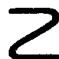
\includegraphics[keepaspectratio]{images/part001_8adf5445.jpg}}

and \(\operatorname{long}(\mathbf{M} / \mathfrak{q}\mathbf{M})\leqslant \operatorname{long}(\mathbf{M} / \mathfrak{x}\mathbf{M})\) ; the three cases

\[
e _ {\mathfrak {q}} (\mathrm{M}) <   \operatorname{long} (\mathrm{M} / \mathfrak {q} \mathrm{M}), e _ {\mathfrak {q}} (\mathrm{M}) = \operatorname{long} (\mathrm{M} / \mathfrak {q} \mathrm{M}), e _ {\mathfrak {q}} (\mathrm{M}) > \operatorname{long} (\mathrm{M} / \mathfrak {q} \mathrm{M})
\]

are possible (p.~106, exerc. 16 and 17).

\specialchapter{Exercises}
\setcounter{exercisesection}{0}

\exercisesection{KRULL DIMENSION OF A RING}

\begin{enumerate}
\def\labelenumi{\arabic{enumi})}
\tightlist
\item
  Let X be a topological space and Y a subspace of X. One says that Y is very dense in X if for every closed subset F of X, F is the closure of F ∩ Y.
\end{enumerate}

\begin{enumerate}
\def\labelenumi{\alph{enumi})}
\item
  For Y to be very dense in X, it is necessary and sufficient that for every nonempty locally closed subset F of X, F ∩ Y be nonempty.
\item
  If Y is very dense in X and Z is a subspace of Y very dense in X, then Z is very dense in X. If Y is very dense in X and F is a locally closed subset of X, then Y ∩ F is very dense in F.
\item
  If Y is very dense in X, one has \(\dim(\mathbf{Y}) = \dim(\mathbf{X})\) .
\end{enumerate}

\begin{enumerate}
\def\labelenumi{\arabic{enumi})}
\setcounter{enumi}{1}
\item
  Let A be a ring and Specmax(A) the set of maximal ideals of A. For Specmax(A) to be very dense in Spec(A), it is necessary and sufficient that A be a Jacobson ring (V, § 3, no. 4). One then has dim Specmax(A) = dim(A).
\item
  Show that if A is a Jacobson ring, A{[}{[}X{]}{]} is not a Jacobson ring. (Compare Specmax(A) and Specmax(A{[}{[}X{]}{]}).)
\item
  \begin{enumerate}
  \def\labelenumii{\alph{enumii})}
  \tightlist
  \item
    Show that one can associate in a unique way to every ordered set E an element of \(\{-\infty\}\cup\mathbf{N}\cup\{+\infty\}\) , denoted dev(E) (deviation of E), such that the following properties are satisfied:
  \end{enumerate}
\end{enumerate}

\(\alpha)\) We have \(\operatorname{dev}(\mathbf{E}) = -\infty\) if and only if the relation \(a \leqslant b\) in \(\mathbf{E}\) implies \(a = b\) .

β) Let n be a positive integer. The deviation of E is ≤ n if and only if, for every infinite decreasing sequence \((a_{k})_{k\in\mathbb{N}}\) of elements of E, one has \(\text{dev}([a_{k}, a_{k-1}]) \leqslant n - 1\) for all sufficiently large k.

\begin{enumerate}
\def\labelenumi{\alph{enumi})}
\setcounter{enumi}{1}
\item
  For one to have \(\text{dev}(\mathbf{E}) \leqslant 0\) , it is necessary and sufficient that every strictly decreasing sequence of elements of E be stationary. One has \(\text{dev}(\mathbf{N}) = 0\) , \(\text{dev}(\mathbf{Z}) = 1\) , \(\text{dev}(\mathbf{Q}) = +\infty\) .
\item
  If E and F are ordered sets and \(f: \mathbf{E} \to \mathbf{F}\) is a strictly increasing map, one has \(\operatorname{dev}(\mathbf{E}) \leqslant \operatorname{dev}(\mathbf{F})\) . We have \(\operatorname{dev}(\mathbf{E} \times \mathbf{F}) = \sup(\operatorname{dev}(\mathbf{E}), \operatorname{dev}(\mathbf{F}))\) .
\item
  Let S(E) be the set of infinite increasing stationary sequences of elements of E, ordered by the product order. Then one has \(\operatorname{dev}(\mathbf{S}(\mathbf{E})) = \operatorname{dev}(\mathbf{E}) + 1\) .
\end{enumerate}

\begin{enumerate}
\def\labelenumi{\arabic{enumi})}
\setcounter{enumi}{4}
\tightlist
\item
  If A is a ring (not necessarily commutative), M a left A-module, one denotes by Kdev(M) the deviation of the set of submodules of M, ordered by inclusion. One sets \(Kdev(A) = Kdev(A_s)\).
\end{enumerate}

\begin{enumerate}
\def\labelenumi{\alph{enumi})}
\tightlist
\item
  If N is a submodule of an A-module M, one has
\end{enumerate}

\[
\operatorname{Kdev} (\mathbf {M}) = \sup (\operatorname{Kdev} (\mathbf {N}), \operatorname{Kdev} (\mathbf {M} / \mathbf {N}))  .
\]

\begin{enumerate}
\def\labelenumi{\alph{enumi})}
\setcounter{enumi}{1}
\item
  Suppose A is commutative. If p and q are two prime ideals of A such that p ⊂ q and p ≠ q, one has dev(A/p) \textgreater{} dev(A/q). (Use the ideals p + Ax, where x is an element of q - p.) Deduce that dim(A) ≤ Kdev(A).
\item
  Suppose A is commutative and noetherian. Prove that one has dim(A) = Kdev(A) (reason by induction on dim(A), assuming that Kdev(B) ≤ dim(B) for every commutative noetherian ring B such that dim(B) \textless{} dim(A); let S be the set of s ∈ A that belong to none of the prime ideals p of A such that dim(A) = dim(A/p); show that, for every finitely generated A-module M such that \(S^{-1}M = 0\) , one has \(\mathrm{Kdev}(\bar{\mathrm{M}}) < \dim(\mathrm{A})\) using the fact that \(S^{-1}A\) is artinian, deduce that \(\mathrm{Kdev}(\mathrm{A}) \leqslant \dim(\mathrm{A})\) . Prove that we have \(\dim(\mathrm{M}) = \mathrm{Kdev}(\mathrm{M})\) for every finitely generated A-module M.
\end{enumerate}

6). a) Let A be a Noetherian (commutative) ring, m an ideal of A contained in the radical of A, and gr(A) the graded ring associated with the m-adic filtration of A. Associate to each ideal of A an ideal of gr(A), and deduce from this that Kdev(A) ≤ Kdev(gr(A)) (cf. Exercise 4, c)). Consequently, one has dim(A) ≤ dim(gr(A)) (Exercise 5, c)).

\begin{enumerate}
\def\labelenumi{\alph{enumi})}
\setcounter{enumi}{1}
\tightlist
\item
  Assume now that m = xA, where x belongs to the radical of A. Show that gr(A) is isomorphic to a quotient of the graded algebra (A/m)[T]. Show that the ordered set F of graded ideals of (A/m) {[}T{]} is isomorphic to the set of increasing sequences of ideals of A/m; deduce from this (exerc. 4, d)) that one has dev(F) = Kdev(A/(x)) + 1, then dim(A) ≤ dim(A/m) + 1.
\end{enumerate}

\begin{enumerate}
\def\labelenumi{\arabic{enumi})}
\setcounter{enumi}{6}
\tightlist
\item
  Let A be the ring of germs at 0 of functions of class \(C^\infty\) on \(\mathbf{R}_{+}\). We propose to show that the ring A is of infinite dimension. We denote by C the algebra of functions of class \(C^\infty\) on \(\mathbf{R}_{+}\) , and let F be the ideal formed by the functions vanishing in a neighborhood of 0, so that \(A = C / F\) .
\end{enumerate}

\begin{enumerate}
\def\labelenumi{\alph{enumi})}
\item
  Let \((x_{n})_{n\in \mathbb{N}}\) be a strictly decreasing sequence, tending to 0, of elements of \(\mathbf{R}_{+}\) , and let \(\mathfrak{U}\) be an ultrafilter on \(\mathbf{N}\) finer than the filter of complements of finite sets. Show that the set \(\mathbf{J}_1\) of \(f\in \mathbf{C}\) such that the set of \(n\in \mathbf{N}\) such that \(f(x_{n}) = 0\) belongs to \(\mathfrak{U}\) is a prime ideal of \(\mathbf{C}\) .
\item
  We denote by \(\tau_{n}(f)\) the function \(x\mapsto f(x + x_{n})\) . Show that if J is a prime ideal of C, the set \(\varphi(J)\) of \(f\) such that the set of \(n\in\mathbf{N}\) with \(\tau_{n}f\in\mathbf{J}\) belongs to \(\mathfrak{U}\) is a prime ideal of C.
\item
  One defines a sequence \(\mathbf{I}_n\) of ideals of C by \(\mathbf{I}_0 = \mathbf{J}_1\) , \(\mathbf{I}_{n+1} = \varphi(\mathbf{I}_n)\) . Show that \((\mathbf{I}_n)_{n\in\mathbb{N}}\) is a strictly decreasing sequence of prime ideals of C containing F.
\end{enumerate}

\begin{enumerate}
\def\labelenumi{\arabic{enumi})}
\setcounter{enumi}{7}
\item
  Let X be a topological space. Show that the map \(x \mapsto \dim_x(X)\) from X to \(\overline{\mathbf{R}}\) is upper semicontinuous.
\item
  Let A be a ring, p a prime ideal of A, and M a finitely generated A-module. Show that one has:
\end{enumerate}

\[
\dim_ {\mathbf {A} _ {\mathfrak {p}}} (\mathbf {M} _ {\mathfrak {p}}) + \dim_ {\mathbf {A} / \mathfrak {p}} (\mathbf {M} / \mathfrak {p} \mathbf {M}) \leqslant \dim_ {\mathbf {A}} (\mathbf {M}).
\]

\begin{enumerate}
\def\labelenumi{\arabic{enumi})}
\setcounter{enumi}{9}
\tightlist
\item
  A ring A is said to be equidimensional if all irreducible components of Spec(A) have the same dimension. Let A be a ring and n an integer. The following conditions are equivalent:
\end{enumerate}

\begin{enumerate}
\def\labelenumi{\alph{enumi})}
\tightlist
\item
  every chain of prime ideals of A is contained in a chain of length n;
\item
  for every maximal ideal m of A, the ring A \(_{m}\) is equidimensional, catenary, and of dimension n.
\end{enumerate}

\begin{enumerate}
\def\labelenumi{\arabic{enumi})}
\setcounter{enumi}{10}
\tightlist
\item
  Let \((\mathbf{A}_{i}, f_{ij})\) be an inductive system of rings relative to a filtered ordered set I, with inductive limit A. Show that one has \(\dim(\mathbf{A}) \leqslant \lim.\inf\dim(\mathbf{A}_{i})\) and that one has equality when the homomorphisms \(f_{ij}\) are faithfully flat. Give an example where the homomorphisms \(f_{ij}\) are flat and where one has \(\dim(\mathbf{A}) < \lim.\inf\dim(\mathbf{A}_{i})\) (take I = N, \(A_{n} = Z[n^{-1}]\) , A = Q).
\end{enumerate}

Let A be a ring, and let I and J be two ideals of A. Suppose that for every maximal ideal m of A, we have IA \(_{m}\) = JA \(_{m}\) . Deduce from this that I = J.

\begin{enumerate}
\def\labelenumi{\alph{enumi})}
\setcounter{enumi}{1}
\item
  Let A be a ring such that, for every maximal ideal m of A, the ring \(\mathrm{A}_{\mathfrak{m}}\) is Noetherian and such that, for every nonzero element \(f\) of A, there exist only finitely many maximal ideals of A containing \(f\) . Then A is Noetherian. (Let \(a\) be an ideal of A. We will first show that there exists a finite family \((x_1, ..., x_n)\) of elements of \(a\) such that the maximal ideals of A that contain \(\{x_1, ..., x_n\}\) contain \(a\). We will then construct a finite family of elements \(y_1, ..., y_l\) such that for every maximal ideal m of A, \(\{y_1, ..., y_l\}\) generates the ideal \(a\mathrm{A}_{\mathfrak{m}}\) of \(\mathrm{A}_{\mathfrak{m}}\) . We conclude by using a).
\item
  Let A be a semi-local ring such that, for every maximal ideal m, the ring \(A_{m}\) is Noetherian. Then A is Noetherian.
\end{enumerate}

\begin{enumerate}
\def\labelenumi{\arabic{enumi})}
\setcounter{enumi}{12}
\item
  Let K be a field, \((n_{r})_{r\geqslant1}\) a strictly increasing sequence of integers \textgreater0; for every integer \(i\geqslant0\) , denote by \(p_{i}\) the ideal of the ring \(\mathrm{K}[(\mathrm{X}_{j})_{j\in\mathbb{N}}]\) generated by the \(X_{j}\) for \(n_{1}+\cdots+n_{i}\leqslant j<n_{1}+\cdots+n_{i}+n_{i+1}\) , and let S be the set of elements of \(\mathrm{K}[(\mathrm{X}_{j})]\) that belong to none of the \(p_{i}\). Then the ring \(S^{-1}K[(X_{j})]\) is Noetherian and of infinite dimension (use Exercise 12 to show that \(S^{-1}K[(X_{j})]\) is Noetherian) \(^{1}\) .
\item
  Let V be a discrete valuation ring, and let \(\pi\) be a uniformizer of V. In the ring V{[}T{]}, the ideal \(m_1 = (\pi T - 1)\) is maximal and of height 1, the ideal \(m_2 = (\pi) + (T)\) is maximal and of height 2. The fields V{[}T{]}/ \(m_1\) and V{[}T{]}/ \(m_2\) are isomorphic to the field of fractions of V and to the residue field of V, respectively. One has \(\dim(\mathrm{V}[T]) = 2\), but \(\dim(\mathrm{V}[T]/m_1) + \dim(\mathrm{V}[T]_{m_1}) = 1\) and \(\dim(\mathrm{gr}_{m_1}(\mathrm{V}[T])) = 1\).
\end{enumerate}

With the notation of the preceding exercise, suppose that the residue field and the field of fractions of the ring V are isomorphic (this is the case, for example, when \(\mathrm{V} = k[[\mathrm{U}]]\) , the field \(k\) being the field of fractions of a ring of formal power series in infinitely many indeterminates with coefficients in a field). Let \(\sigma\) be an isomorphism of \(\mathrm{V[T] / m_1}\) onto \(\mathrm{V[T] / m_2}\) . Let C denote the subring of \(\mathrm{V[T]} = \mathrm{E}\) consisting of the elements of E whose classes modulo \(m_1\) and \(m_2\) correspond under \(\sigma\) . Show that C is Noetherian and that \(m_1m_2 = m_1 \cap m_2\) is a maximal ideal of C. Show that E is the integral closure of C (noting that \(\mathrm{E} = \mathrm{C} + \mathrm{C}\cdot(\pi T - 1)\) and that \((\pi T - 1)^2 + (\pi T - 1)\) belongs to C).

Let \(\mathring{\mathrm{A}}\) be the local ring \(\mathbf{C}_{\mathfrak{m}_1\mathfrak{m}_2}\) . Then A is an integral domain of dimension 2, hence catenary; the integral closure \(\mathbf{B} = \mathbf{E} \otimes_{\mathbb{C}} \mathbf{A}\) of \(\mathring{\mathrm{A}}\) is a semi-local Noetherian ring having exactly two maximal ideals \(\mathfrak{n}_1\) and \(\mathfrak{n}_2\) , and we have \(\dim(\mathbf{B}_{\mathfrak{n}_1}) = 1\) , \(\dim(\mathbf{B}_{\mathfrak{n}_2}) = 2\) .

¶ 16) We keep the notation of the preceding exercise, and we identify B with the quotient of the polynomial ring A{[}U{]} by the prime ideal \(\mathfrak{p}\) generated by \(U^2 + U - \pi T(\pi T - 1)\). Let \(\mathfrak{q}_i\) be the ideal of A{[}U{]} such that \(\mathfrak{n}_i = \mathfrak{q}_i/\mathfrak{p}\). Then \(\operatorname{ht}(\mathfrak{q}_i) = 3\), \(\operatorname{ht}(\mathfrak{p}) = 1\), and the chain \(\mathfrak{p} \subset \mathfrak{q}_1\) is saturated. In particular, A{[}U{]} and A{[}U{]}\(_{\mathfrak{q}_1}\) are not catenary.

\begin{enumerate}
\def\labelenumi{\arabic{enumi})}
\setcounter{enumi}{16}
\tightlist
\item
  \begin{enumerate}
  \def\labelenumii{\alph{enumii})}
  \tightlist
  \item
    Let A be an integral domain and \(f \in \mathrm{A}[\mathrm{T}], f \neq 0\). Show that there exists a maximal ideal m of \(\mathrm{A}[\mathrm{T}]\) such that \(f \notin \mathfrak{m}\) (take a maximal ideal containing T.f-1).
  \end{enumerate}
\end{enumerate}

\begin{enumerate}
\def\labelenumi{\alph{enumi})}
\setcounter{enumi}{1}
\tightlist
\item
  Let A be a ring. Show that one has dim(Specmax(A{[}T{]})) \(\geqslant\) dim(A) + 1. (Let \(\mathfrak{p}_0\subset \mathfrak{p}_1\subset \cdots \subset \mathfrak{p}_n\) be a chain of prime ideals of A. Consider the chain
\end{enumerate}

\[
\mathfrak {p} _ {0} [ \mathrm{T} ] \subset \mathfrak {p} _ {1} [ \mathrm{T} ] \subset \mathfrak {p} _ {2} [ \mathrm{T} ] \dots \subset \mathfrak {p} _ {n} [ \mathrm{T} ] \subset (\mathfrak {p} _ {n}, \mathrm{T})
\]

of prime ideals of A{[}T{]} and let us set

\[
\left\{ \begin{array}{l} \mathrm{U} _ {i} = \mathrm{V} (\mathfrak {p} _ {i} [ \mathrm{T} ]) \cap \operatorname{Specmax} (\mathrm{A} [ \mathrm{T} ]), \quad 0 \leqslant i \leqslant n \\ \mathrm{U} _ {n + 1} = \mathrm{V} (\mathfrak {p} _ {n}, \mathrm{T}) \cap \operatorname{Specmax} (\mathrm{A} [ \mathrm{T} ]). \end{array} \right.
\]

Show, using \(a\) ) that \((\mathrm{U}_i)_{0 \leqslant i \leqslant n+1}\) is a strictly increasing sequence of irreducible closed subsets of Specmax (A{[}T{]}).

\begin{enumerate}
\def\labelenumi{\alph{enumi})}
\setcounter{enumi}{2}
\tightlist
\item
  Let \(k\) be a field, and let S be the subset of \(k[\mathrm{X}, \mathrm{Y}]\) formed by the elements of the form \(1 + \mathrm{X}g(\mathrm{X}, \mathrm{Y})\) , and let \(\mathrm{A} = \mathrm{S}^{-1}k[\mathrm{X}, \mathrm{Y}]\) .
\end{enumerate}

Show that one has dim(Specmax(A)) = 1 and dim(Spec(A)) = 2. Generalize to the case of several indeterminates.

\begin{enumerate}
\def\labelenumi{\alph{enumi})}
\setcounter{enumi}{3}
\item
  Show that for every pair of integers \(0 \leqslant n < m\) , there exists a Noetherian ring A such that \(\dim(\text{Specmax}(A)) = n\) and \(\dim(\text{Specmax}(A[T])) = m\) .
\item
  Let A be the Noetherian ring defined in exerc. 13. Show that one has dim(Specmax(A)) = 1 and dim(Specmax(A{[}T{]})) = \(\infty\) .
\end{enumerate}

\exercisesection{DIMENSION OF ALGEBRAS}

\begin{enumerate}
\def\labelenumi{\arabic{enumi})}
\item
  Let V be a discrete valuation ring, with fraction field K, and let n be an integer. Let A be the subring of the polynomial ring \(K[X_{1},...,X_{n}]\) formed by the polynomials whose constant term lies in V. The canonical homomorphism from V to A satisfies property (PM) and the canonical homomorphism \(V/m_{V} \rightarrow A/m_{V}A\) is an isomorphism. Moreover, one has \(\dim(A) \geqslant n + 1\) and \(\dim(V) = 1\) . As soon as \(n \geqslant 1\) , one therefore has \(\dim(A) > \dim(V) + \dim(A/m_{V}A)\) . Show that A is not Noetherian. Using formal series, construct an analogous example where A is local and not Noetherian.
\item
  Let V be a discrete valuation ring, with fraction field K and residue field k. Denote by A the ring \(K \times k\) and \(\rho : V \to A\) the homomorphism deduced from the canonical homomorphisms from V to K and k. The homomorphism \(\rho\) is injective, the map \(^{a}\rho : \text{Spec}(A) \to \text{Spec}(V)\) is surjective, A is a finitely generated V-algebra, and we have \(\dim(A) < \dim(V)\) .
\item
  Let A be an integral domain of dimension 1, and let \(\mathfrak{p}_0 \subset \mathfrak{p}_1 \subset \mathfrak{p}_2\) be three distinct nonzero prime ideals of A{[}X{]}. Show that we have \(\mathfrak{p}_0 \cap \mathbf{A} = \{0\}\) , \(\mathfrak{p}_1 = (\mathfrak{p}_1 \cap \mathbf{A})\cdot\mathrm{A}{[}X{]}\), and that \(\mathfrak{p}_2\) is a maximal ideal of A{[}X{]}.
\item
  Let A be a local integrally closed ring, \(m_A\) its maximal ideal and K its field of fractions. For every element x of K, we denote by A{[}x{]} the sub-A-algebra of K generated by x. Let x be an element of K* such that \(x^{-1}\) does not belong to A. Let A{[}X{]} be the ring of polynomials in one indeterminate X, with coefficients in A, and \(\varphi\) the evaluation map P \(\mapsto\) P(x) of A{[}X{]} on A{[}x{]}.
\end{enumerate}

\begin{enumerate}
\def\labelenumi{\alph{enumi})}
\item
  The kernel of \(\varphi\) is the ideal Q generated by the polynomials of the form \(aX + b\) , where \(a, b \in A\) and \(ax + b = 0\) . (If \(\mathrm{P}(X) = \sum_{i=0}^{n} a_i X^i\) is such that \(\mathrm{P}(x) = 0\) , note that then \(-b_0 = a_0 x\) is integral over \(A\) therefore belongs to \(A\) .)
\item
  The ideal \(m_A A[x]\) of \(A[x]\) is prime, and it is maximal if and only if \(x\) belongs to \(A\) .
\end{enumerate}

\begin{enumerate}
\def\labelenumi{\arabic{enumi})}
\setcounter{enumi}{4}
\item
  Let A be an integrally closed ring with fraction field K. Given a prime ideal p of A, and an element x of K such that \(x \notin A_{p}\) , and \(x^{-1} \notin A_{p}\) the ideal pA{[}x{]} of A{[}x{]} is prime; we have: pA{[}x{]} ∩ A = p and the canonical homomorphism (A/p){[}X{]} → A{[}x{]}/pA{[}x{]} is an isomorphism.
\item
  \begin{enumerate}
  \def\labelenumii{\alph{enumii})}
  \tightlist
  \item
    Using the previous exercises, show that if A is an integral domain of dimension 1, then dim(A{[}X{]}) = 2 if and only if all the localizations at a prime ideal of the integral closure of A are valuation rings.
  \end{enumerate}
\end{enumerate}

\begin{enumerate}
\def\labelenumi{\alph{enumi})}
\setcounter{enumi}{1}
\tightlist
\item
  Show that if one has \(\dim(\mathbf{A}) = n\) and \(\dim(\mathbf{A}[\mathbf{X}]) > n + 1\), there exists a prime ideal \(\mathfrak{p}\) of A such that \(\operatorname{ht}(\mathfrak{p}) = 1\) and either \(\dim(\mathbf{A}_{\mathfrak{p}}[\mathbf{X}]) > 2\) or \(\dim((\mathbf{A}/\mathfrak{p})[\mathbf{X}]) > \dim(\mathbf{A}/\mathfrak{p}) + 1\) .
\item
  Deduce that if A is Prüferian (VII, § 2, exerc. 12), then we have \(\dim(\mathbf{A}[\mathbf{X}_1, ..., \mathbf{X}_n]) = \dim(\mathbf{A}) + n\) , for every integer \(n \geqslant 0\) .
\end{enumerate}

\begin{enumerate}
\def\labelenumi{\arabic{enumi})}
\setcounter{enumi}{6}
\item
  Let B be an integrally closed ring, with field of fractions L. We set \(d = \dim(B)\) and \(t = \dim(B[X])\) . Let L' be a non-trivial extension of L in which L is algebraically closed, and let V be a discrete valuation ring (which is not a field) having L' as its residue field. We denote by K the field of fractions of V and by A the set of elements of V whose image in L' under the canonical homomorphism V → L' belongs to B. The ring A is integrally closed with field of fractions K. Let p denote the kernel of the surjective homomorphism A → B. Show that every non-zero prime ideal of A contains p, whence dim(A) = dim(B) + 1. Considering an element x of V whose image in L' does not belong to L, show that the ring of fractions A \(_{p}\) is not a valuation ring, and that pA \(_{p}\) {[}x{]} is not minimal among the non-zero prime ideals of A \(_{p}\) {[}x{]}. Using exercise 6, deduce that one has dim(A{[}x{]}) ≥ t + 2. Conclude that one has dim(A{[}x{]}) = t + 2 by a direct argument. Finally show that for every pair (d, t) of integers with d + 1 ≤ t ≤ 2d + 1, there exists an integral domain A of dimension d such that dim(A{[}X{]}) = t.
\item
  Show that the polynomial ring A{[}X{]} is a faithfully flat A-module, that for every maximal ideal m of A one has dim(A{[}X{]}/mA{[}X{]}) = 1, and deduce from the preceding exercise the existence of ring homomorphisms \(\rho: A \to B\) satisfying condition (PM) and such that \(\dim(B) > \dim(A) + \inf_{\mathfrak{m}\in S}\dim(B/\mathfrak{m}B)\) (where S is the set of maximal ideals of A).
\item
  Let A be an integral domain and B an integral domain containing A and integral over A. Let p be a prime ideal of A such that the integral closure of the ring of fractions \(A_{p}\) is a local ring. For every prime ideal q of B lying over p, one has ht(q) = ht(p) (use V, § 2, n° 1, prop. 2).
\end{enumerate}

¶ 10) a) Let A be an integral domain, K its field of fractions, and m a positive integer. Let \(t_1, \ldots, t_m\) be elements of K and \(\varphi: \mathrm{A}[\mathrm{X}_1, \ldots, \mathrm{X}_m] \to \mathrm{A}[t_1, \ldots, t_m]\) the unique homomorphism of A-algebras such that \(\varphi(\mathrm{X}_i) = t_i\) . Show that the height of the kernel ideal of \(\varphi\) is equal to m. b) Deduce that for every \(m\) -tuple ( \(t_1, \ldots, t_m\) ) of elements of K, one has \(\dim(\mathrm{A}[t_1, \ldots, t_m]) \leqslant \dim(\mathrm{A}[\mathrm{X}_1, \ldots, \mathrm{X}_m]) - m\) .

¶ 11) Let A be an integral domain and K its field of fractions. Let \((0) \subset \mathfrak{p}_1 \subset \ldots \subset \mathfrak{p}_h\) be a chain of prime ideals of A. Show that there exists a valuation ring V of K and a chain of prime ideals \((0) \subset \mathfrak{q}_1 \subset \ldots \subset \mathfrak{q}_h\) of V such that \(\mathfrak{q}_i \cap A = \mathfrak{p}_i\) . (Proceed by induction on \(h\) , reducing to the case where A is a local ring and using, for the case \(h = 1\) , exercise 7 of VI, § 1.)

\begin{enumerate}
\def\labelenumi{\arabic{enumi})}
\setcounter{enumi}{11}
\tightlist
\item
  \begin{enumerate}
  \def\labelenumii{\alph{enumii})}
  \tightlist
  \item
    Let A and K be as above, let B be an integral domain containing A and integral over A, and let L be the fraction field of B. Let \(k \geqslant 0\) be an integer. If, for every \(m\)-tuple \((t_1, \ldots, t_m)\) of elements of L, we have \(\dim(A[t_1, \ldots, t_m]) \leqslant k\), then, for every \(m\)-tuple \((u_1, \ldots, u_m)\) of elements of L, we have \(\dim(B[u_1, \ldots, u_m]) \geqslant k\). b) Let p be a prime ideal of A. Show that if, for all \(m\)-tuples \((t_1, \ldots, t_m)\) of elements of K, one has \(\dim(A[t_1, \ldots, t_m]) \leqslant k\), then we have for all \(m\)-tuples \((s_1, \ldots, s_m)\) of elements of the field of fractions of A/p, the inequality \(\dim((A/p)[s_1, \ldots, s_m]) \leqslant k - \text{ht}(p)\) .
  \end{enumerate}
\end{enumerate}

¶ 13) Let A be an integral domain and K its field of fractions. For every integer \(k \geqslant 0\) , the following properties are equivalent:

\begin{enumerate}
\def\labelenumi{(\roman{enumi})}
\item
  Every subring B of K containing A has dimension \(\leqslant k\) .
\item
  Every valuation ring V of K containing A has dimension \(\leqslant k\) .
\item
  For every choice of \(k\) elements \(t_1, \ldots, t_k\) of \(\mathbf{K}\) , one has \(\dim(A[t_1, \ldots, t_k]) \leqslant k\) .
\item
  We have \(\dim(A[X_1, ..., X_m]) \leqslant k + m\) for every integer \(m \geqslant 0\) .
\end{enumerate}

\begin{enumerate}
\def\labelenumi{\arabic{enumi})}
\setcounter{enumi}{13}
\tightlist
\item
  Let A be an integral domain, with field of fractions K, and \(m \in N\). Show that we have
\end{enumerate}

\[
\dim (\mathrm{A} [ \mathrm{X} _ {1},..., \mathrm{X} _ {m} ]) = m + \sup \left\{\dim (\mathrm{A} [ t _ {1},..., t _ {m} ]) | t _ {i} \in \mathrm{K}, 1 \leqslant i \leqslant m \right\}.
\]

(We will use Exercise 10). More generally, if F is a field, an extension of K, show that we have

\[
\dim \left(\mathrm{A} \left[ \mathrm{X} _ {1}, \dots , \mathrm{X} _ {m} \right]\right) = \sup \left\{\dim (\mathrm{A} \left[ t _ {1}, \dots , t _ {m} \right]) \mid t _ {i} \in \mathrm{F}, 1 \leqslant i \leqslant m \right\} + \sup (0, m - \deg . \operatorname{tr} _ {\mathbf {K}} (\mathrm{F})).
\]

\begin{enumerate}
\def\labelenumi{\arabic{enumi})}
\setcounter{enumi}{14}
\tightlist
\item
  With the notations of the previous exercises, show that if for some integer \(k \geqslant 0\) , one has \(\dim(A[X_1, ..., X_m]) \geqslant k + m + 1\) for a suitable integer \(m\), one has the inequality \(\dim(A[X_1, ..., X_k]) \geqslant 2k + 1\) .
\end{enumerate}

  ¶ 16) Let A be an integral domain and K its field of fractions. One calls the valuative dimension of A and denotes it by \(\dim_{\mathrm v}(\mathrm A)\) the real number \(\sup_{A \subset V \subset K} \dim(V)\) , where V ranges over the set of valuation rings of K containing A

\begin{enumerate}
\def\labelenumi{\alph{enumi})}
\item
  Show that one has \(\dim(\mathrm A) \leqslant \dim_{\mathrm v}(\mathrm A)\) (exercise 11).
\item
  If A is Prüferian (VII, § 2, exerc. 12), show that one has \(\dim(\mathrm A) = \dim_{\mathrm v}(\mathrm A)\).
\item
  Show that, for all \(m \in \mathbf{N}\) , one has
\end{enumerate}

\[
\dim_ {\mathbf {v}} (\mathrm{A} [ \mathrm{X} _ {1},..., \mathrm{X} _ {m} ]) = \dim_ {\mathbf {v}} (\mathrm{A}) + m.
\]

(Note that a valuation ring is Prüferian, and one will use b) and exercise 6, p.~84.)

\begin{enumerate}
\def\labelenumi{\alph{enumi})}
\setcounter{enumi}{3}
\tightlist
\item
  Show that if one has \(\dim_{\mathrm v}(\mathrm A) = s < \infty\), one has, for every integer \(m \geqslant s - 1\) the equality
\end{enumerate}

\[
\dim (\mathrm{A} [ \mathrm{X} _ {1},..., \mathrm{X} _ {m} ]) = m + s.
\]

\begin{enumerate}
\def\labelenumi{\alph{enumi})}
\setcounter{enumi}{4}
\tightlist
\item
  Let \(s \in \mathbf{N}\) . Show that we have \(\dim_{\mathrm{v}}(\mathbf{A}) = s\) if and only if \(\dim(\mathbf{A}[\mathbf{X}_1, ..., \mathbf{X}_s]) = 2s\) (using \(d\) ) and Exercises 13 and 14).
\end{enumerate}

Deduce that, for every integral Noetherian ring A, one has \(\dim(\mathrm{A}) = \dim_{\mathrm{v}}(\mathrm{A})\).

\begin{enumerate}
\def\labelenumi{\arabic{enumi})}
\setcounter{enumi}{16}
\tightlist
\item
  Let A be an integral domain. Set \(n_k(A) = \dim(A[X_1, ..., X_k])\) for every integer \(k \geqslant 0\). Let D be the set of sequences of integers \((n_i)_{i \geqslant 0}\) such that there exists an integral domain A with \(n_i = n_i(A)\) for every integer \(i \geqslant 0\) .
\end{enumerate}

\begin{enumerate}
\def\labelenumi{\alph{enumi})}
\tightlist
\item
  Prove the inequalities
\end{enumerate}

\[
\sup \left(n _ {0} (\mathrm{A}) + i + 1, n _ {i} (\mathrm{A}) + 1\right) \leqslant n _ {i + 1} (\mathrm{A}) \leqslant \inf \left(2 n _ {i} (\mathrm{A}) + 1, 2 ^ {i + 1} \left(n _ {0} (\mathrm{A}) + 1\right) - 1\right).
\]

\begin{enumerate}
\def\labelenumi{\alph{enumi})}
\setcounter{enumi}{1}
\tightlist
\item
  Show that the only sequence of integers beginning with 1, 2 and belonging to D is the sequence \(n_{i}=i+1\) . (Let A be such that \(n_{0}(A)=1\) , \(n_{1}(A)=2\) . By exerc. 6, p.~84, the integral closure of A is Prüferian. Use exerc. 6, c), p.~84 to conclude.)\\
\item
  Prove the inequalities
\end{enumerate}

\[
n _ {0} (\mathrm{A}) + i \leqslant n _ {i} (\mathrm{A}) \leqslant (n _ {0} (\mathrm{A}) + 1) (i + 1) - 1.
\]

Deduce that if one has \(n_0(\mathbf{A}) = 0\) , then we have \(n_i(\mathbf{A}) = i\) for every \(i \in \mathbf{N}\) .

\begin{enumerate}
\def\labelenumi{\alph{enumi})}
\setcounter{enumi}{3}
\item
  Show that the sequence of differences \(n_{i+1}(\mathbf{A}) - n_i(\mathbf{A})\) is stationary.
\item
  We use the notations of exerc. 7, p.~84. Let δ be the transcendence degree of L' over L. Then:
\end{enumerate}

\begin{enumerate}
\def\labelenumi{(\roman{enumi})}
\item
  If \(\delta = 0\) , one has \(n_i(A) = n_i(B) + 1\) for every \(i\) .
\item
  If \(1 \leqslant \delta < \infty\) , one has \(n_i(A) = n_i(B) + i + 1\) for \(0 \leqslant i \leqslant \delta\) and \(n_i(A) = n_i(B) + \delta + 1\) for \(i \geqslant \delta\) .
\item
  If \(\delta = \infty\) , one has \(n_i(A) = n_i(B) + i + 1\) for every \(i\) .
\end{enumerate}

(For a characterization of the elements of D, one may consult T. Parker, Amer. J. Math., 97 (1975), pp. 308–311.)

* 18) Let A (resp. B) denote the algebra C \(\{z_{1}, z_{2}, z_{3}\}\) (resp. C \(\{u, v\}\) ) of convergent series in the variables \(z_{1}, z_{2}, z_{3}\) (resp. \(u, v\) ) and \(\varphi: A \to B\) the unique algebra homomorphism such that \(\varphi(z_{1}) = uv\) , \(\varphi(z_{2}) = v(e^{u} - 1)\) , \(\varphi(z_{3}) = v\) . Show that \(\varphi\) is injective, and that we have dim(A) = 3 and dim(B) = 2. *

\exercisesection{DIMENSION OF NOETHERIAN RINGS}

\begin{enumerate}
\def\labelenumi{\arabic{enumi})}
\tightlist
\item
  Let A be a ring, and let U be an open subset of Spec(A).
\end{enumerate}

\begin{enumerate}
\def\labelenumi{\alph{enumi})}
\item
  Show that the map \(\mathfrak{p} \mapsto \mathrm{V}(\mathfrak{p}) \cap \mathrm{U}\) induces a bijection from U onto the set of closed irreducible subsets of U.
\item
  Show that dim(U) is the upper bound of the set of lengths of chains of prime ideals of A belonging to U.
\item
  Let \(\Phi\) be the set of minimal prime ideals of A belonging to U. Show that one has
\end{enumerate}

\[
\dim (\mathrm{U}) = \sup _ {\mathfrak {p} \in \Phi} \dim (\mathrm{V} (\mathfrak {p}) \cap \mathrm{U}).
\]

\begin{enumerate}
\def\labelenumi{\alph{enumi})}
\setcounter{enumi}{3}
\item
  Assume henceforth that A is local and U ≠ Spec(A). If A is Noetherian, establish the equality \(\dim(\mathrm{U}) = \sup_{\mathfrak{p}\in\Phi}(\dim(\mathrm{A}/\mathfrak{p}) - 1)\).
\item
  Let h be an integer such that 0 \textless{} h \textless{} dim(A). Let \(E_{h}\) be the set of prime ideals \(p \in U\) such that \(ht(p) = h\) and \(\dim(A/p) = \dim(A) - h\) . If A is Noetherian, show that \(E_{h}\) is infinite. Show that \(E_{h}\) may be finite when A is not Noetherian (take for A a valuation ring of height 2, for U the open \(\text{Spec}(A) - \{m_{A}\}\) , and choose h = 1).
\end{enumerate}

\begin{enumerate}
\def\labelenumi{\arabic{enumi})}
\setcounter{enumi}{1}
\item
  Let A be a Noetherian integral domain. Suppose that A is not a field and that the field of fractions of A is a finitely generated A-algebra. Then A is semi-local and of dimension 1. (Show that there exists a nonzero, non-invertible element \(f\) of A such that \(A[f^{-1}]\) is a field, and reduce to proving that \(\dim(A/(f)) = 0\) ; if it were otherwise, \(A/(f)\) would possess a prime ideal of height 1 whose inverse image p in A would be a prime ideal of height 2; but the local ring \(A_p\) of dimension 2 could have only a finite number of prime ideals, contrary to prop. 6 of § 3, no. 3.)
\item
  \begin{enumerate}
  \def\labelenumii{\alph{enumii})}
  \tightlist
  \item
    Let A be a Noetherian local ring, and let p be a prime ideal of A. Prove the inequality \(\dim_{\mathfrak{p}}(\mathbf{A}) \geqslant \mathrm{ht}(\mathfrak{p}) + \dim(\mathbf{A}/\mathfrak{p}) - 1\) .
  \end{enumerate}
\end{enumerate}

\begin{enumerate}
\def\labelenumi{\alph{enumi})}
\setcounter{enumi}{1}
\tightlist
\item
  Prove that there exists a Noetherian local ring R of dimension 3 having a prime ideal q such that ht(q) = 1 and dim(R/q) = 1. (Use exerc. 16, p.~83, by taking \(\mathbf{R} = \mathbf{A}[\mathbf{U}]_{\mathbf{q}}\) , and q = pR.) Let \(f \in \mathfrak{m}_{\mathbb{R}} - \mathfrak{q}\) ; show that \(\dim(\mathbf{R}_{f}) = 2\) (use exerc. 1, p.~86); we therefore have \(\dim_{\mathfrak{q}}(\mathbf{R}) = 2\) whereas \(\operatorname{ht}(\mathfrak{q}) + \dim(\mathbf{R}/\mathfrak{q}) - 1 = 1.\)
\end{enumerate}

\begin{enumerate}
\def\labelenumi{\arabic{enumi})}
\setcounter{enumi}{3}
\item
  Let \(k\) be a field, and let \(n\) be an integer \(\geqslant 1\). For each integer \(r \in [0, n]\) , let \(M_r\) be the vector subspace of \(k(X_1, ..., X_n)\) generated by the monomials \(X_1^{\alpha_1}\ldots X_r^{\alpha_r}\) with \(\alpha_1, ..., \alpha_r\) in \(Z\) and \(\alpha_r > 0\) . Put \(a_r = M_r + \cdots + M_n\) , for \(0 \leqslant r \leqslant n + 1\) . Then \(a_0\) is a subring of \(k(X_1, ..., X_n)\) , and the \(a_r\) are prime ideals of \(a_0\) . Put \(A = (a_0)_{a_1}\) and \(p_r = (a_r)_{a_1}\) for \(1 \leqslant r \leqslant n + 1\) . Show that the only prime ideals of the local ring \(A\) are the \(p_r\) , and that one has \(ht(p_r) = n + 1 - r\) and \(dim(A) = n\) . Moreover \(p_1\) is principal.
\item
  Let \(\rho: \mathbf{A} \to \mathbf{B}\) be a local homomorphism of complete Noetherian local rings, such that \([\kappa(\mathbf{B}): \kappa(\mathbf{A})] < \infty\) . Put \(n = \dim(\mathbf{B}/\mathfrak{m}_{\mathbf{A}}\mathbf{B})\) ; show that there exists a local A-homomorphism \(u: \mathbf{A}[[\mathbf{T}_1, ..., \mathbf{T}_n]] \to \mathbf{B}\) which makes B a \(\mathbf{A}[[\mathbf{T}_1, ..., \mathbf{T}_n]]\) -finite algebra. (Lift in B a maximal secant sequence of \(\mathbf{B}/\mathfrak{m}_{\mathbf{A}}\mathbf{B}\) and use III, § 3, exerc. 18.)
\item
  Let \(k\) be a field and A the ring of formal power series \(k[[X_1, X_2]]\) . Consider an ideal \(\mathfrak{n}\) of A containing a power of the maximal ideal \(\mathfrak{m}\) of A, and the ideal I generated by \((X_1 - X_2)\mathfrak{n}\) . Let M be the module A/I. Show that the sequence \((X_1)\) is secant for M without being completely secant for M.
\item
  Let A be a local, integral, Noetherian, non-catenary ring of dimension 3 (exerc. 16, p.~83), p ⊂ A a prime ideal such that ht(p) = 1, dim(A/p) = 1. Show that there exists an element x ∈ p such that p is minimal among the prime ideals containing Ax. Deduce that V(x) has an irreducible component of dimension 1.
\end{enumerate}

\exercisesection{HILBERT-SAMUEL SERIES}

\begin{enumerate}
\def\labelenumi{\arabic{enumi})}
\tightlist
\item
  Let \(\Gamma\) be a commutative group and let H be a graded ring of type \(\Gamma\) (A, II, p.~164).
\end{enumerate}

For \(\gamma\in\Gamma\) , we denote by H \(_{\gamma}\) the homogeneous component of degree \(\gamma\) of H. We assume that H is generated by H \(_{0}\) and a finite family (x \(_{i}\) ) \(_{i\in I}\) of homogeneous elements of degree \(\neq0\) . We denote by \(\gamma_{i}\) the degree of x \(_{i}\) . For every commutative group K, we denote by K{[}{[}Γ{]}{]} the product group K \(^{\Gamma}\) and we denote by \(\sum_{\gamma\in\Gamma}m_{\gamma}\text{T}^{\gamma}\) the element (m \(_{\gamma}\) ) of K \(^{\Gamma}\) . We denote by K{[}Γ{]} the subgroup K \(^{(\Gamma)}\) of K{[}{[}Γ{]}. We endow K{[}{[}Γ{]}{]} with its natural structure as a module over the algebra Z{[}Γ{]} of the group Γ. Finally, let C be a hereditary set of classes of H₀-modules (A, VIII, § 10, no. 1, def. 1) and let K(C) be the corresponding Grothendieck group (loc. cit., no. 2). For every H₀-module E of type C, we denote {[}E{]} its class in K(C).

\begin{enumerate}
\def\labelenumi{\alph{enumi})}
\tightlist
\item
  Suppose \(\mathbf{H}_0\) is Noetherian, and let \(\mathbf{M}\) be a finitely generated graded H-module such that for every \(\gamma \in \Gamma\) , the \(\mathbf{H}_0\) -module \(\mathbf{M}_{\gamma}\) is of type C. Show that the element \(\prod_{i \in I} (1 - T^{\gamma_i}) \sum_{\gamma \in \Gamma} [\mathbf{M}_{\gamma}] T^{\gamma}\) of
\end{enumerate}

\(K(\mathbb{C})[[\Gamma]]\) belongs to \(K(\mathbb{C})[\Gamma]\) .

\begin{enumerate}
\def\labelenumi{\alph{enumi})}
\setcounter{enumi}{1}
\tightlist
\item
  Suppose now that \(\Gamma = \mathbf{Z}^s\) , \(\mathrm{H}_{\gamma} = 0\) and \(\mathbf{M}_{\gamma} = 0\) for \(\gamma \notin \mathbf{N}^s\) , and that the \(\gamma_i\) are basis vectors of \(\mathbf{Z}^s\) ; denoting by \(a_k\) the number of \(\gamma_i\) that are equal to the \(k\) th basis vector, prove that one has
\end{enumerate}

\[
\prod_ {k = 1} ^ {s} (1 - \mathrm{T} _ {k}) ^ {a _ {k}} \sum_ {\gamma \in \mathbf {Z} ^ {s}} [ \mathrm{M} _ {\gamma} ] \mathrm{T} ^ {\gamma} = \sum_ {\gamma} m _ {\gamma} \mathrm{T} ^ {\gamma}
\]

where \(\mathbf{T} = (\mathrm{T}_{1},\dots,\mathrm{T}_{s})\) , and \((m_{\gamma})\) is a finitely supported family. Deduce the existence of elements \(c_{\boldsymbol{b}}\in\mathrm{K}(\mathbb{C})\), for \(\boldsymbol{b}\in\mathbf{Z}^{s}\), all but finitely many of which are zero, such that, for \(\gamma\in\mathbf{N}^{s}\) sufficiently large, one has

\[
[ \mathbf {M} _ {\gamma} ] = \sum_ {\boldsymbol {b}} c _ {\boldsymbol {b}} \mathbf {B} _ {\boldsymbol {b}} (\gamma)
\]

where

\[
\mathrm{B} _ {b} (\gamma) = \prod_ {j = 1} ^ {s} \frac {(\gamma_ {j} + 1) \dots (\gamma_ {j} + b _ {j})}{b _ {j} !},
\]

the sum being taken over the elements b of \(Z^{s}\) satisfying \(b_{i} < a_{i}\) for \(1 \leqslant i \leqslant s\) .

\begin{enumerate}
\def\labelenumi{\arabic{enumi})}
\setcounter{enumi}{1}
\tightlist
\item
  Let \(f: \mathbf{Z} \to \mathbf{Z}\) be a map. Show that the following three properties are equivalent:
\end{enumerate}

\begin{enumerate}
\def\labelenumi{\alph{enumi})}
\item
  There exists \(n_0, n_1\) in \(\mathbf{Z}\) and \(\mathrm{P}\) in \(\mathbf{Q}[\mathrm{T}]\) such that \(f(n) = 0\) for \(n \leqslant n_1\) and \(f(n) = \mathrm{P}(n)\) for \(n \geqslant n_0\) .
\item
  There exists a finitely supported family \((a_i)_{i\in \mathbf{Z}}\) of elements of \(\mathbf{Z}\) such that \(f(n) = \sum_{i\in \mathbf{Z}}a_i\left[ \begin{array}{cc}n + i\\ i \end{array} \right]\) for every \(n\in \mathbf{Z}\) .
\item
  There exists \(r \in \mathbf{Z}\) and \(Q \in \mathbf{Z}[T, T^{-1}]\) such that \(\sum_{n \in \mathbf{Z}} f(n) T^n = (1 - T)^r Q(T)\) .
\end{enumerate}

Then we say that \(f\) is polynomial at infinity.

Generalize to the case of maps from Z into an arbitrary Z-module.

\begin{enumerate}
\def\labelenumi{\arabic{enumi})}
\setcounter{enumi}{2}
\tightlist
\item
  \begin{enumerate}
  \def\labelenumii{\alph{enumii})}
  \tightlist
  \item
    Give an example of a graded algebra H of type Z, over a field K, generated by a finite number of homogeneous elements of degrees \textgreater{} 0, and such that the map \(n \mapsto \dim_{\mathbf{K}} \mathrm{H}_{n}\) is not polynomial at infinity.
  \end{enumerate}
\end{enumerate}

\begin{enumerate}
\def\labelenumi{\alph{enumi})}
\setcounter{enumi}{1}
\tightlist
\item
  With the notations and hypotheses of th. 1 of § 4, no. 2, let D be the lcm of the \(d_{i}\). Show that H is a finitely generated module over the ring \(\mathrm{H}_{0}[(\mathrm{X}_{i}^{\mathrm{D}/d_{i}})_{i\in\mathbb{I}}]\) .
\end{enumerate}

Deduce that for every \(n_{0}\in\mathbf{N}\) the series \(\sum_{n\in\mathbf{Z}}\mathrm{long}_{\mathrm{H}_{0}}(\mathbf{M}_{n_{0}+n\mathbf{D}})\mathbf{T}^{n}\) is of the form \(\frac{\mathbf{P}_{n_{0}}(\mathbf{T})}{(1-\mathbf{T})^{c}}\) where \(c=\mathrm{Card}(\mathbf{I})\) and \(\mathbf{P}_{n_{0}}(\mathbf{T})\in\mathbf{Q}[\mathbf{T},\mathbf{T}^{-1}]\) . Deduce that the map \(n\mapsto\mathrm{long}_{\mathrm{H}_{0}}(\mathbf{M}_{n_{0}+n\mathbf{D}})\) is polynomial at infinity.

\begin{enumerate}
\def\labelenumi{\arabic{enumi})}
\setcounter{enumi}{3}
\tightlist
\item
  Let us place ourselves in the situation of Th. 1 of § 4, No. 2, and denote by C the set of isomorphism classes of finitely generated graded H-modules with components of finite length over \(\mathbf{H}_0\), and by \(\mathrm{K}(\mathbb{C})\) the corresponding Grothendieck group.
\end{enumerate}

\begin{enumerate}
\def\labelenumi{\alph{enumi})}
\tightlist
\item
  For every H-module M as above, show that there exists an \(H_{0}\)-graded module of finite length \(M_{0}\) and a surjective graded homomorphism \(p:H\otimes_{H_{0}}M_{0}\to M\). Deduce from this that every H-module M as above admits a graded resolution (A, X, p.~56) by H-modules:
\end{enumerate}

\[
\dots \rightarrow \mathrm{H} \otimes_ {\mathrm{H} _ {0}} \mathrm{M} _ {1} \rightarrow \mathrm{H} \otimes_ {\mathrm{H} _ {0}} \mathrm{M} _ {0} \rightarrow \mathrm{M} \rightarrow 0
\]

where, for all \(i\), \(M_{i}\) is an \(H_{0}\)-graded module of finite length.

\begin{enumerate}
\def\labelenumi{\alph{enumi})}
\setcounter{enumi}{1}
\item
  Using a Koszul resolution of the H-module \(\mathbf{H}_0\) (A, X, p.~152), show that for every graded H-module M, \(\mathrm{Tor}_j^{\mathrm{H}}(\mathrm{H}_0,\mathrm{M})\) is canonically endowed with a grading, that \(\mathrm{Tor}_j^{\mathrm{H}}(\mathrm{H}_0,\mathrm{M}) = 0\) for \(j > \mathrm{Card}(\mathrm{I})\), and that \(\mathrm{Tor}_j^{\mathrm{H}}(\mathrm{H}_0,\mathrm{P}\otimes_{\mathrm{H}_0}\mathrm{H})\) is an \(\mathbf{H}_0\)-module of finite length for every \(j\) when P is an \(\mathbf{H}_0\)-module of finite length.
\item
  Show that for every \(j\) , \(\mathrm{Tor}_{j}^{\mathrm{H}}(\mathrm{H}_{0}, \mathrm{M})\) is an \(\mathrm{H}_{0}\)-graded module of finite length when M is of type C. (One may show this by induction on \(j\) . If \(j = 0\) , use a) and b). In the general case, use an exact sequence \(0 \to \mathbf{N} \to \mathbf{H} \otimes_{\mathrm{H}_{0}} \mathbf{M}_{0} \to \mathbf{M} \to 0\) , the induction hypothesis and b).)
\item
  For every H-module M of type C, we set
\end{enumerate}

\[
e (\mathbf {M}) = \sum_ {p \in \mathbf {Z}} \sum_ {j = 0} ^ {\infty} (- 1) ^ {j} [ \operatorname{Tor} _ {j} ^ {\mathrm{H}} (\mathrm{H} _ {0}, \mathbf {M}) _ {p} ] \mathrm{T} ^ {p},
\]

  thus obtaining an element of \(\mathbf{K}(\mathcal{C}_{0})[\mathrm{T},\mathrm{T}^{-1}]\) where \(\mathbf{K}(\mathcal{C}_{0})\) is the Grothendieck group of \(\mathrm{H}_{0}\)-modules of finite length. Show that \(\mathbf{M}\mapsto e(\mathbf{M})\) is additive on exact sequences of graded H-modules, and consequently \(\mathbf{M}\mapsto e(\mathbf{M})\) determines a group homomorphism

\[
e: \mathrm{K} (\mathfrak {C}) \to \mathrm{K} (\mathfrak {C} _ {0}) [ \mathrm{T}, \mathrm{T} ^ {- 1} ].
\]

For every \(H_{0}\) -graded module P of finite length, we set

\[
\tau (\mathrm{P}) = [ \mathrm{H} \otimes_ {\mathrm{H} _ {0}} \mathrm{P} ] \in \mathrm{K} (\mathbb {C}).
\]

Show that \(\mathbf{P} \mapsto \tau(\mathbf{P})\) is additive on exact sequences and that consequently \(\mathbf{P} \mapsto \tau(\mathbf{P})\) determines a homomorphism between the corresponding Grothendieck groups

\[
\tau : \mathrm{K} (\mathbb {C} _ {0}) [ \mathrm{T}, \mathrm{T} ^ {- 1} ] \rightarrow \mathrm{K} (\mathbb {C}).
\]

Show that \(e\) and \(\tau\) are mutually inverse group isomorphisms. (One will first show that \(e \circ \tau\) is the identity. To prove the assertion, it therefore suffices to show that \(\tau\) is surjective, that is, to show that for every H-module M of type C, {[}M{]} belongs to the image of \(\tau\) . One will note that M admits a finite filtration whose successive quotients are annihilated by a maximal ideal of \(H_0\) and that an H-module M of type C, annihilated by a maximal ideal m of \(H_0\) , admits a finite graded resolution by finitely generated free H/mH-modules (A, X, p.~56).)

\begin{enumerate}
\def\labelenumi{\alph{enumi})}
\setcounter{enumi}{4}
\tightlist
\item
  Let M be an H-module of type C. Show that in K(C) one has
\end{enumerate}

\[
[ \mathbf {M} ] = \sum_ {i \geqslant 0} (- 1) ^ {i} [ \mathrm{H} \otimes_ {\mathrm{H} _ {0}} \operatorname{Tor} _ {i} ^ {\mathrm{H}} (\mathrm{H} _ {0}, \mathbf {M}) ].
\]

\begin{enumerate}
\def\labelenumi{\alph{enumi})}
\setcounter{enumi}{5}
\tightlist
\item
  Let \(\Gamma\) be a commutative group and \(\Phi : K(\mathbb{C}) \to \Gamma\) a group homomorphism. For every \(H_0\) -module P of finite length, set
\end{enumerate}

\[
\psi (\mathrm{P}) = \Phi ([ \mathrm{H} \otimes_ {\mathrm{H} _ {0}} \mathrm{P} ]).
\]

Show that for every H-module M of type C, one has

\[
\Phi ([ \mathbf {M} ]) = \sum_ {j \geqslant 0} (- 1) ^ {j} \psi (\operatorname{Tor} _ {j} ^ {\mathrm{H}} (\mathrm{H} _ {0}, \mathbf {M})).
\]

In particular, with the notations of remark 4 of § 4, no. 2, show that one has

\[
\mathrm{Q} _ {\mathbf {M}} = \sum_ {j = 0} ^ {r} (- 1) ^ {j} \mathrm{P} _ {\mathrm{T} _ {j}},
\]

and consequently that

\[
c _ {\mathbf {M}} = \sum_ {j = 0} ^ {r} (- 1) ^ {j} \mathrm{long} _ {\mathrm{H} _ {0}} (\mathrm{Tor} _ {j} ^ {\mathrm{H}} (\mathrm{H} _ {0}, \mathbf {M})).
\]

\begin{enumerate}
\def\labelenumi{\alph{enumi})}
\setcounter{enumi}{6}
\tightlist
\item
  Using the preceding results, give a new proof of th. 1 of § 4, no. 1.
\item
  Let Γ be a commutative group. Describe all additive maps M ↦ Φ(M) on H-modules of type C with values in Γ, in terms of maps from Specmax(H₀) × Z to Γ.
\item
  Assume that H₀ is a field. Let A be a ring. Describe all additive maps \(M\mapsto C(M)\) with values in \(A\) such that \(C(M)\cdot C(N) = \sum_j(-1)^j C(\operatorname{Tor}_{j}^{\mathrm{H}}(M,N))\) for every pair M and N of finitely generated graded H-modules.
\end{enumerate}

\begin{enumerate}
\def\labelenumi{\arabic{enumi})}
\setcounter{enumi}{4}
\tightlist
\item
  \begin{enumerate}
  \def\labelenumii{\alph{enumii})}
  \tightlist
  \item
    Let H be a graded ring of type N, such that \(H_{0}\) is a field and H is a finitely generated \(H_{0}\) -algebra. Let M and N be two finitely generated graded H-modules. Set \(T_{i} = \operatorname{Tor}_{i}^{\mathrm{H}}(\mathbf{M}, \mathbf{N})\) . Prove the equality
  \end{enumerate}
\end{enumerate}

\[
\sum_ {i = 0} ^ {\infty} (- 1) ^ {i} \mathrm{P} _ {\mathrm{T} _ {i}} = \frac {\mathrm{P} _ {\mathrm{M}} \cdot \mathrm{P} _ {\mathrm{N}}}{\mathrm{P} _ {\mathrm{H}}}.
\]

\begin{enumerate}
\def\labelenumi{\alph{enumi})}
\setcounter{enumi}{1}
\tightlist
\item
  Let A be a Noetherian local ring, and M and N two A-modules. Show that if, for \(m \in Z\) and \(i \geqslant 1\) , \(\operatorname{Tor}_{i}^{\operatorname{gr}_{m}(A)}(\operatorname{gr}_{m}(M), \operatorname{gr}_{m}(N))\) is zero, then one has \(\operatorname{Tor}_{i}^{A}(M, N) = 0\) for \(i \geqslant 1\) and \(H_{M \otimes_{A} N, m} = \frac{H_{M, m} \cdot H_{N, m}}{H_{A, m}}\) for \(m \in Z\) .
\end{enumerate}

\begin{enumerate}
\def\labelenumi{\arabic{enumi})}
\setcounter{enumi}{5}
\tightlist
\item
  Let H be a graded ring of type Z, such that \(H_{n} = \{0\}\) for n \textless{} 0, that \(H_{0}\) is an Artinian local ring and that H is a finitely generated \(H_{0}\) -algebra. Let L. be a bounded complex of finitely generated free graded H-modules (cf. A, X, p.~56). Thus for each i, \(L_{i}\) is isomorphic to an H-module of the form \(\bigoplus_{j=1}^{r_{i}} H(-n_{ij})\) , with \(n_{ij} \in Z\) , where \(H(-k)\) is the graded H-module such that \(H(-k)_{n} = H_{n-k}\) . For every finitely generated graded H-module M, denote by \(G_{M} \in Q[T]\) the unique polynomial such that there exists an integer \(n_{1} \geqslant 0\) satisfying
\end{enumerate}

\[
\mathrm{G} _ {\mathrm{M}} (n) = \sum_ {i <   n} \operatorname{long} _ {\mathrm{H} _ {0}} (\mathrm{M} _ {i}), \quad \text {for} \quad n \geqslant n _ {1}.
\]

Prove the relation

\[
\sum_ {i \geqslant 0} (- 1) ^ {i} \mathrm{G} _ {\mathrm{H} _ {i} (\mathrm{L.})} = \sum_ {k \geqslant 0} \frac {(- 1) ^ {k}}{k !} \rho_ {k} \frac {\partial^ {k} \mathrm{G} _ {\mathrm{H}}}{\partial \mathrm{T} ^ {k}}
\]

where \(\rho_{k} = \sum_{i\geqslant 0}(-1)^{i}\sum_{j = 1}^{r_{i}}n_{ij}\) , the \(n_{ij}\) being the degrees associated with \(\mathbf{L}_i\) , and where \(\mathrm{H}_i(\mathrm{L.})\) denotes the homology of the complex \(\mathrm{L.}\).

¶ 7) a) Let l be an integer ≥ 1 and n ∈ N. Show that there exists a unique decreasing sequence of integers: \(a_{l,l}(n) \geqslant a_{l,l-1}(n) \geqslant \cdots \geqslant a_{l,1}(n) \geqslant 0\) such that

\[
n = \sum_ {i = 1} ^ {l} \binom {a _ {l, i} (n) + i - 1} {i}.
\]

Show that one has \(n \leqslant m\) if and only if \((a_{l,l}(n), a_{l,l-1}(n), ..., a_{l,1}(n))\) is less than or equal to \((a_{l,l}(m), ..., a_{l,1}(m))\) for the lexicographic order.

One sets

\[
\partial_ {l} (n) = \sum_ {i = 1} ^ {l} \binom {a _ {l, i} (n) + i} {i + 1},
\]

and, for \(l \geqslant 2\) , denote by \(\partial_l^*(n)\) the smallest integer \(p\) such that \(\partial_{l-1}(p) \geqslant n\) .

Compute \(a_{l+1,i}(\partial_l(n)), a_{l-1,i}(\partial_l^*(n))\) in terms of the \(a_{l,i}(n)\) .

\begin{enumerate}
\def\labelenumi{\alph{enumi})}
\setcounter{enumi}{1}
\tightlist
\item
  One says that a map H:N → N is a Macaulay function if
\end{enumerate}

\[
\left\{ \begin{array}{l l} \mathrm{H} (0) = 1, \\ \mathrm{H} (l + 1) \leqslant \partial_ {l} (\mathrm{H} (l)) & \text {for all} \quad l \geqslant 1. \end{array} \right.
\]

Show that this is equivalent to saying that

\[
\left\{ \begin{array}{l} \mathrm{H} (0) = 1, \\ \partial_ {l} ^ {*} \mathrm{H} (l) \leqslant \mathrm{H} (l - 1) \quad \text {for all} \quad l \geqslant 2. \end{array} \right.
\]

Let H : N → N be a Macaulay function. Show that only two cases are possible: α) There exists r ∈ N such that H(j) = 0 for all j ≥ r.

β) There exists \(r \in \mathbf{N}\) and a finite sequence of integers

\[
b _ {0} \geqslant b _ {1} \geqslant \dots \geqslant b _ {r} \geqslant 0
\]

such that for all \(j \geqslant r\) , one has

\[
(*) \quad \mathrm{H} (j) = \sum_ {n = 0} ^ {r} \binom {b _ {n} - n + j} {b _ {n}}.
\]

Show that \(r\) and the sequence \(b_0 \geqslant b_1 \geqslant \cdots \geqslant b_r \geqslant 0\) are uniquely determined by the function \(H\). We set \(d(H) = 0\) in case \(\alpha\) and \(d(H) = b_0 + 1\) in case \(\beta\), so that \(d(H) - 1\) is the degree of the polynomial (*) in the variable \(j\). Let \(a(H) \frac{j^{d(H)-1}}{(d(H) - 1)!}\) be the term of highest degree of the polynomial (*). Show that \(a(H)\) is an integer \(> 0\).

Show that a polynomial in one variable \(j\) with coefficients in \(\mathbf{Q}\) , which takes integer values on integers and is strictly positive for \(j\) large enough, is not necessarily of the form (*).

\begin{enumerate}
\def\labelenumi{\alph{enumi})}
\setcounter{enumi}{2}
\tightlist
\item
  Let H: N → N be a Macaulay function. We set
\end{enumerate}

\[
\mathrm{S} _ {\mathrm{H}} (\mathrm{T}) = \sum_ {n = 0} ^ {\infty} \mathrm{H} (n) \mathrm{T} ^ {n},
\]

so that \(S_{H}(T) \in Z[[T]]\) . Show that \(S_{H}(T) \in Z[T]\) or else that there exists a finite sequence of integers

\[
c _ {0} \geqslant c _ {1} \geqslant \dots \geqslant c _ {r} > 0
\]

uniquely determined by H, and a polynomial \(P \in Z[T]\) such that one has

\[
(* *) \mathrm{S} _ {\mathrm{H}} (\mathrm{T}) = \sum_ {n = 0} ^ {r} \frac {\mathrm{T} ^ {n}}{(1 - \mathrm{T}) ^ {c _ {n}}} + \mathrm{P}.
\]

Show that \(c_0 = d(\mathbf{H})\) and that \(a(\mathbf{H})\) is the number of integers \(c_i\) such that \(c_i = d(\mathbf{H})\) .

The rational fraction \(\sum_{n=0}^{r}\frac{T^n}{(1-T)^{c_n}}\) is called the asymptotic expansion of \(H\). Let \(A_1, ..., A_d\) be integers, with \(A_d \neq 0\), such that the rational fraction

\[
\sum_ {n = 1} ^ {d} \frac {\mathrm{A} _ {n}}{(1 - \mathrm{T}) ^ {n}} - \mathrm{S} _ {\mathrm{H}} (\mathrm{T})
\]

is a polynomial. Show that the sequence \((\mathrm{A}_{n})_{1\leq n\leq d}\) is uniquely determined by, and uniquely determines, the asymptotic expansion of \(H\). In particular, we have \(d=d(\mathrm{H})\), \(\mathrm{A}_{d}=a(\mathrm{H})\). Examine the case \(d(\mathrm{H})=2\) in more detail.

\begin{enumerate}
\def\labelenumi{\alph{enumi})}
\setcounter{enumi}{3}
\tightlist
\item
  Let \(\mathbf{H}:\mathbf{N}\to\mathbf{N}\) be a Macaulay function. Show that the following conditions are equivalent:
\end{enumerate}

\begin{enumerate}
\def\labelenumi{(\roman{enumi})}
\item
  \(\partial_l^*\mathrm{H}(l) = \mathrm{H}(l - 1)\) for every \(l\geqslant 2\)
\item
  H is the smallest Macaulay function having the same asymptotic expansion as H.
\end{enumerate}

Such Macaulay functions are said to be extremal. Let \(c_{0} \geqslant c_{1} \geqslant \cdots \geqslant c_{r} > 0\) be a sequence of integers. Show that there exists one and only one extremal Macaulay function whose asymptotic expansion is \(\sum_{n=0}^{r} \frac{\mathrm{T}^{n}}{(1 - \mathrm{T})^{c_{n}}}\) . Show that, if H is an extremal Macaulay function, then one has \(\mathrm{H}(1) = d(\mathrm{H})\) or \(\mathrm{H}(1) = d(\mathrm{H}) + 1\). Deduce from this that for every Macaulay function H, one has \(\mathrm{H}(1) \geqslant d(\mathrm{H})\) .

\begin{enumerate}
\def\labelenumi{\alph{enumi})}
\setcounter{enumi}{4}
\tightlist
\item
  Let H: N → N be a Macaulay function. Show that the following properties are equivalent:
\end{enumerate}

\begin{enumerate}
\def\labelenumi{(\roman{enumi})}
\tightlist
\item
  we have \(\mathrm{S_H(T)} = \frac{1}{(1 - T)^{d(H)}}\)
\end{enumerate}

\begin{enumerate}
\def\labelenumi{(\roman{enumi})}
\setcounter{enumi}{1}
\item
  \(\mathbf{H}(1) = d(\mathbf{H})\)
\item
  \(\partial_{l}\mathbf{H}(l) = \mathbf{H}(l + 1)\) for every \(l\geqslant 1\)
\end{enumerate}

In particular, any function such that \(\mathrm{H}(1)=d(\mathrm{H})\) is extremal.

\begin{enumerate}
\def\labelenumi{\arabic{enumi})}
\setcounter{enumi}{7}
\tightlist
\item
  Let E be a set. We set \(\mathcal{M}(\mathrm{E}) = \mathbf{N}^{(\mathrm{E})}\) and we denote multiplicatively the composition in \(\mathcal{M}(\mathrm{E})\) . An ideal of \(\mathcal{M}(\mathrm{E})\) is a subset \(I\) of \(\mathcal{M}(\mathrm{E})\) such that \(I\cdot\mathcal{M}(\mathrm{E}) \subset I\) . A staircase of \(\mathcal{M}(\mathrm{E})\) is the complement of an ideal. We denote by \(d: \mathcal{M}(\mathrm{E}) \to \mathbf{N}\) the unique monoid homomorphism such that \(d(x) = 1\) , for all \(x \in \mathrm{E}\) . Let \(\mathrm{A} \subset \mathcal{M}(\mathrm{E})\) . For every \(l \in \mathbf{N}\) , denote by \(\mathrm{A}_l\) the set \(\mathrm{A} \cap d^{-1}(l)\) . We also denote \(\delta \mathrm{A}\) the set of \(m \in \mathcal{M}(\mathrm{E})\) such that, for every element \(x\) of E which divides \(m\) , one has \(m / x \in \mathrm{A}\) and \(d\mathrm{A}\) the set of \(m\) such that there exists an \(x \in \mathrm{E}\) with \(mx \in \mathrm{A}\) .
\end{enumerate}

\begin{enumerate}
\def\labelenumi{\alph{enumi})}
\tightlist
\item
  Show that for every subset A of \(\mathcal{M}(E)\) , one has \(d\delta A \subset A\) and \(A \subset \delta dA\) ; if A and B are two subsets of \(\mathcal{M}(E)\) , the relations \(dA \subset B\) and \(A \subset \delta B\) are equivalent. Show that the following three properties of a subset \(\Delta\) of \(\mathcal{M}(E)\) are equivalent:
\end{enumerate}

\begin{enumerate}
\def\labelenumi{(\roman{enumi})}
\item
  \(\Delta\) is a staircase;
\item
  \(\Delta \supset d\Delta\) ;
\item
  \(\delta \Delta \supset \Delta\) .
\end{enumerate}

\begin{enumerate}
\def\labelenumi{\alph{enumi})}
\setcounter{enumi}{1}
\tightlist
\item
  Let F be a subset of E and identify \(\mathcal{M}(\mathbf{F})\) with its canonical image in \(\mathcal{M}(\mathbf{E})\) . Show that a subset of \(\mathcal{M}(\mathbf{F})\) is a staircase of \(\mathcal{M}(\mathbf{F})\) if and only if it is a staircase of \(\mathcal{M}(\mathbf{E})\) . Show that, for a staircase \(\Delta\) of \(\mathcal{M}(\mathbf{E})\) the following conditions are equivalent:
\end{enumerate}

\begin{enumerate}
\def\labelenumi{(\roman{enumi})}
\item
  \(\Delta_l\) is finite for every \(l \in \mathbf{N}\) ;
\item
  \(\Delta_{1}\) is finite;
\item
  there exists a finite subset F of E such that \(\Delta\subset\mathcal{M}(F)\) .
\end{enumerate}

Such a staircase is said to be of finite type.

\begin{enumerate}
\def\labelenumi{\alph{enumi})}
\setcounter{enumi}{2}
\tightlist
\item
  From now on, we assume that E = N and we set \(\mathcal{M}(E) = \mathcal{M}\) . Let k be a field. We denote by R the graded algebra \(\mathrm{K}^{(\mathcal{M})} = \mathrm{K}[(\mathrm{X}_i)_{i \in \mathbb{N}}]\) . We identify M with the set of monomials in \(\mathrm{K}[(\mathrm{X}_i)_{i \in \mathbb{N}}]\) and, for every subset A of M, we denote by \(k(A)\) the vector subspace of R generated by A. Let I be an ideal of M and \(\Delta\) the complementary staircase. Then \(k(I)\) is an ideal of R and \(k(\Delta)\) is a supplementary subspace of \(k(I)\) . Let \(J \subset R\) be a graded ideal of \(R\). Show that there exists a staircase \(\Delta \subset M\) such that \(k(\Delta)\) is a supplement of \(J\). (Put on \(M\) the reverse lexicographic order for which one has \(X_1^{a_1} \ldots X_n^{a_n} \prec X_1^{b_1} \ldots X_n^{b_n}\) if there exists \(0 \leqslant p \leqslant n\) such that \(a_j = b_j\) for \(j \textgreater{} p\), and \(a_p < b_p\) . Define by induction \(m_1, \ldots, m_p, \ldots\) in \(M\) as follows: for every \(p\), \(m_p\) is the smallest monomial of \(M\) linearly independent of \(m_1, \ldots, m_{p-1}\) modulo \(J\). Let \(\Delta\) be the set of \(m_i\) . Show that \(\Delta\) is a staircase.) Show that such a staircase is of finite type if and only if the algebra \(R/J\) is of finite type over \(k\).
\end{enumerate}

  We use the notation from the previous exercise. We put the lexicographic order on \(M\). Let \(l \in \mathbf{N}\). A subset \(A\) of \(\mathcal{M}_{l}\) is said to be initial if for every \(m \in \mathrm{A}\) , the set

\[
[ m ] = \{m ^ {\prime} \in \mathcal {M} _ {d (m)} | m ^ {\prime} <   m \}
\]

is contained in A.

\begin{enumerate}
\def\labelenumi{\alph{enumi})}
\item
  Let \(l \in \mathbf{N}\) (resp. \(l \in \mathbf{N} - \{0\}\) ) and let \(\mathbf{A} \subset \mathcal{M}_l\) be an initial segment. Show that \(\delta \mathbf{A}\) (resp. \(d\mathbf{A}\) ) is an initial segment of \(\mathcal{M}_{l+1}\) (resp. \(\mathcal{M}_{l-1}\) ). Suppose that \(\mathbf{A}\) has a greatest element \(m = X_1^{a_1} \ldots X_n^{a_n}\) . Determine the greatest element of \(\delta \mathbf{A}\) (resp. \(d\mathbf{A}\) ).
\item
  Let \(l \in \mathbf{N} - \{0\}\) and let \(\mathbf{A} \subset \mathcal{M}_l\) be a nonempty finite initial segment. Let \(\mathrm{X}_{a_l}\) be the largest variable such that \([\mathrm{X}_{a_l}^l] \subset \mathbf{A}\) . Show that every \(m\) in \(\mathbf{A} - [\mathrm{X}_{a_l}^l]\) is equal to 1 or divisible by \(\mathrm{X}_{a_l + 1}\) and that \(\mathrm{A}' = \{m \in \mathcal{M}_{l-1}|m\mathrm{X}_{a_l + 1} \in \mathbf{A} - [\mathrm{X}_{a_l}^l]\}\) is an initial segment of \(\mathcal{M}_{l-1}\). Deduce from the preceding an expression for \(\operatorname{Card}([X_1^{b_1} ... X_n^{b_n}])\) .
\item
  Deduce from the preceding that, for every \(l \in \mathbf{N} - \{0\}\) and every finite initial segment A of \(\mathcal{M}_l\) , one has \(\text{Card}(\delta\text{A}) = \partial_l(\text{Card}(\text{A}))\) , where \(\partial_l\) was defined in exerc. 7. Compute analogously \(\text{Card}(d\text{A})\) .
\item
  For every \(l \in \mathbf{N}\) and every \(n \in \mathbf{N}\) , set
\end{enumerate}

\[
\mu (n) = \inf_{\substack{\mathbf{A}\subset \mathcal{M}_{l}\\ \operatorname{Card}(\mathbf{A}) = n}}\operatorname{Card}(d\mathbf{A}),
\]

and denote by \(m_{n}\) the \(n\) -th monomial of \(\mathcal{M}_{l}\) for the lexicographic order (we set \(m_{0}=1\) ).

For every finite subset A of \(\mathcal{M}_{l}\) , denote by CA the initial segment of \(\mathcal{M}_{l}\) such that \(\mathrm{Card(A)} = \mathrm{Card(CA)}\) . Show that the following three assertions are equivalent:

(MC1) for every \(l \in \mathbf{N}\) and every \(\mathbf{A} \subset \mathcal{M}_l\) , one has \(\mathbf{C}\delta \mathbf{A} \subset \delta \mathbf{CA}\) ;

(MC2) for every \(l \in \mathbf{N}\) and every \(\mathbf{A} \subset \mathcal{M}_l\) , one has \(d\mathbf{CA} \subset \mathbf{CdA}\) ;

(MC3) for every \(l \in \mathbf{N}\) and every \(n \in \mathbf{N}\) , one has \(\operatorname{Card}(d[m_n]) = \mu(n)\) .

\begin{enumerate}
\def\labelenumi{\arabic{enumi})}
\setcounter{enumi}{9}
\tightlist
\item
  We use the notation of the two preceding exercises. Let \(l \in \mathbf{N}\) and \(\mathbf{A} \subset \mathcal{M}_l\) . For every pair \((i, d)\) one sets
\end{enumerate}

\(\mathrm{A}_{(i;d)} = \{m \in \mathrm{A} | m \text{ is divisible by } \mathrm{X}_i^d \text{ and is not divisible by } \mathrm{X}_i^{d+1}\}\)

and we denote by \(C_{(i;d)}A\) the set of \(\operatorname{Card}(A_{(i;d)})\) first elements of \((\mathcal{M}_{l})_{(i;d)}\) (for the lexicographic order). We set \(C_{i}A = \bigcup C_{(i;d)}A\) .

\begin{enumerate}
\def\labelenumi{\alph{enumi})}
\tightlist
\item
  For every \(m \in \mathcal{M}_{l}\) , denote by \(\pi(m)\) the predecessor in \(\mathcal{M}_{l}\) of \(m\) for the reverse lexicographic order, when it exists (i.e., \(m \neq X_{1}^{l}\) ). Let \(i\) be an integer such that \(1 < i\), and let \(a_{i}\) be a strictly positive integer. Show that we have
\end{enumerate}

\[
\begin{array}{c} \pi (X _ {i} ^ {a _ {i}} \dots X _ {p} ^ {a _ {p}}) = X _ {i - 1} X _ {i} ^ {a _ {i} - 1} \dots X _ {p} ^ {a _ {p}} \\ \pi (X _ {1} ^ {a _ {1}} X _ {i} ^ {a _ {i}} \dots X _ {p} ^ {a _ {p}}) = X _ {i - 1} ^ {a _ {i - 1} + 1} X _ {i} ^ {a _ {i} - 1} \dots X _ {p} ^ {a _ {p}}. \end{array}
\]

\begin{enumerate}
\def\labelenumi{\alph{enumi})}
\setcounter{enumi}{1}
\item
  Let \(\mathbf{A} \subset \mathcal{M}_l\) and \(p \geqslant 4\) such that we have \(\mathbf{A} \subset [\mathbf{X}_p^l]\) (i.e., such that the monomials belonging to \(\mathbf{A}\) involve only the variables \(\mathbf{X}_j\) , \(1 \leqslant j \leqslant p\) ). We assume that for every integer \(i\) such that \(1 \leqslant i \leqslant p\) , one has \(\mathbf{A} = \mathbf{C}_i\mathbf{A}\) . Show that \(\mathbf{A} = \mathbf{CA}\) (notations of exerc. 9, d)).
\item
  Let \(\mathbf{A} \subset \mathcal{M}_l\) such that \(\mathbf{A} \subset [\mathbf{X}_3^l]\) and that \(\mathbf{A} = \mathbf{C}_i\mathbf{A}\) for \(i = 1, 2, 3\) . Put \(\mathbf{A} = \bigcup_{k=0} \mathbf{B}_k\mathbf{X}_3^{k}\) with \(\mathbf{B}_k \subset [\mathbf{X}_2^{l-k}]\) and \(b(k) = \text{Card}(\mathbf{B}_k)\) . Show that \(\mathbf{B}_k\) is an initial segment of \(\mathcal{M}_{l-k}\) and that \(0 \leqslant b(0) \leqslant l + 1\) , \(b(k+1) < b(k)\) if \(b(k) \neq 0\) , and that \(k \mapsto b(k)\) is decreasing. Examine the converse of this assertion. Let \(\mu\) be the number of integers \(k\) such that \(b(k) = l + 1 - k\) . Show that \(\text{Card}(d\mathbf{A}) = (\text{Card}(\mathbf{A})) - \mu\) .
\end{enumerate}

¶ 11) We propose to prove assertions MC1, MC2, MC3 of exercise 9, d) (Macaulay's theorem). Let \(l \in \mathbf{N}\) , \(\mathbf{A} \subset \mathcal{M}_l\) , and let \(p\) be the smallest integer such that \(\mathbf{A} \subset [\mathbf{X}_p^l]\) . We shall prove MC2 by induction on \(p\) .

\begin{enumerate}
\def\labelenumi{\alph{enumi})}
\item
  Prove the theorem for \(p = 1\) and \(p = 2\) .
\item
  Using the induction hypothesis, show that for all \(i \leqslant p\) , \(dC_{i}A \subset C_{i}dA\) (notations of Exerc. 8).
\item
  One sets \(\mathbf{A}^1 = \mathbf{A}\) , \(\mathbf{A}^{j+1} = \mathbf{C}_i\mathbf{A}^j\) where \(i \equiv j \mod p\) and \(1 \leqslant i \leqslant p\) . Show that for \(j\) sufficiently large one has \(\mathbf{A}^{j+1} = \mathbf{A}^j\) . (For every \(a \in \mathcal{M}_l\) , let \(n(a) \in \mathbf{N}\) denote the rank of \(a\) in the lexicographic order and set \(n(\mathbf{A}) = \sum_{a \in \mathbf{A}} n(a)\) . Show that \(n(\mathbf{A}^{j+1}) \leqslant n(\mathbf{A}^j)\) and that \(n(\mathbf{A}^{j+1}) = n(\mathbf{A}^j)\) if and only if \(\mathbf{A}^{j+1} = \mathbf{A}^j\) .)
\item
  Prove the theorem in the general case. (A subset \(A \subset [X_{p}^{l}] \subset M_{l}\) is said to be minimal if \(\operatorname{Card}(dA) \leqslant \operatorname{Card}(dA')\) for the subsets \(A' \subset [X_{p}^{l}]\) such that \(\operatorname{Card}(A') = \operatorname{Card}(A)\). It is a matter of showing that if A is minimal, then CA is minimal. Let A be minimal. Using b), show that \(C_{i}A\) is minimal for all \(i \leqslant p\) . Deduce, using the notation of c), that \(A^{j}\) is minimal for all j. Deduce from c) that there exists a minimal B such that \(\operatorname{Card}(B) = \operatorname{Card}(A)\) and \(C_{i}B = B\) for \(1 \leqslant i \leqslant p\) . In the case p = 3, use exerc. 10, c) to conclude. In the case \(p \geqslant 4\) using Exerc. 10, b) to deduce that \(B = CA\) .
\end{enumerate}

¶ 12) Let H : N → N be a map and let k be a field. We propose to prove the equivalence of the following properties:

\begin{enumerate}
\def\labelenumi{(\roman{enumi})}
\item
  H is a Macaulay function (p.~90, exerc. 7).
\item
  There exists a staircase of finite type (p.~92, exerc. 8) \(\Delta \subset \mathcal{M}\) such that for all \(l \in \mathbf{N}\) , one has \(\mathrm{H}(l) = \mathrm{Card}(\Delta_l)\) .
\item
  There exists a graded \(k\)-algebra \(\mathbf{A}\) , of type \(\mathbf{N}\) generated by a finite number of its elements of degree 1, such that for every \(l\) , one has \(\mathrm{H}(l) = \dim_k A_l\) .
\end{enumerate}

\begin{enumerate}
\def\labelenumi{\alph{enumi})}
\item
  To prove (ii) \(\Leftrightarrow\) (iii), we will use exerc. 8, c).
\item
  We prove (i) \(\Rightarrow\) (ii). Let H be a Macaulay function. For every \(l\) , let \(\Delta_l \subset \mathcal{M}_l\) be the initial part such that \(\operatorname{Card}(\Delta_l) = \mathrm{H}(l)\) and let us set \(\Delta = \bigcup_{l} \Delta_l\) . To show that \(\Delta\) is a staircase, we will use exerc. 9, c).
\item
  We prove (ii) \(\Rightarrow\) (i). Let \(\Delta\) be a staircase. To show that \(\mathbf{H}: l \mapsto \operatorname{Card}(\Delta_l)\) is a Macaulay function, we will use Macaulay's theorem (MC1) (exerc. 11) and exerc. 9, c) \(^{1}\) .
\end{enumerate}
% semantic-fragments: legacy-input-seam
\relax{}
\exercisesection{REGULAR LOCAL RINGS}

\begin{enumerate}
\def\labelenumi{\arabic{enumi})}
\item
  Let A be a ring, S a multiplicative subset of A. Show that one has \(\mathrm{dh}(\mathrm{S}^{-1}\mathrm{A}) \leqslant \mathrm{dh}(\mathrm{A})\) (A, X, p.138, def. 2). (Take resolutions of the \(S^{-1}A\) -modules by projective A-modules and localize.)
\item
  Let A be a Noetherian ring and B a faithfully flat A-algebra. Then we have \(\mathrm{dh(A)}\leqslant \mathrm{dh(B)}\).
\end{enumerate}

3) Let A be a Noetherian local ring. We propose to show that A is regular if and only if dh(A) is finite.

\begin{enumerate}
\def\labelenumi{\alph{enumi})}
\tightlist
\item
  Suppose dh(A) is finite. To show that A is regular, use A, X, p.208, exerc. 13.
\item
  Suppose A is regular. Let x be a completely secant family generating m\_A. Then, the Koszul complex associated with x is a finite resolution of A/m\_A by free A-modules. Then apply A, X, p.203, exerc. 16.
\end{enumerate}

\begin{enumerate}
\def\labelenumi{\arabic{enumi})}
\setcounter{enumi}{3}
\item
  Let A be a regular Noetherian local ring. Then we have \(\dim(A) = \mathrm{dh}(A)\) (To show that we have \(\mathrm{dh}(A) \leqslant \dim(A)\), use the Koszul complex associated with a system of coordinates. Then determine the groups \(\operatorname{Ext}_{A}^{i}(\kappa_{A}, \kappa_{A})\).)
\item
  Let A be a regular Noetherian local ring, and let p be a prime ideal of A. Then \(A_{p}\) is regular (use Exerc. 1 and Exerc. 3).
\item
  A Noetherian ring A is said to be regular if for every prime ideal p of A, the local ring \(A_{p}\) is regular.
\end{enumerate}

\begin{enumerate}
\def\labelenumi{\alph{enumi})}
\item
  Let A be a Noetherian ring. Then A is regular if and only if \(A_{m}\) is regular for every maximal ideal m of A (use Exercise 5).
\item
  Let A be a Noetherian ring. Show that A is regular of finite dimension if and only if dh(A) is finite (use Exercise 4).
\item
  Show that the ring described in Exercise 13, p.83 is regular of infinite dimension.
\item
  Let A be a regular Noetherian ring, and S a multiplicative subset. Show that \(\mathbf{S}^{-1}\mathbf{A}\) is regular.
\item
  Let A be a regular Noetherian ring. Show that A{[}X{]} is regular. (Reduce by localization to the case where dh(A) is finite. Use A, X, p. 143, th. 1, and b).
\end{enumerate}

\(^{1}\) For further details on this exercise, one may consult R. Stanley, The Hilbert function of a graded algebra, Advances in Math., 28 (1978), pp. 57–83.

\begin{enumerate}
\def\labelenumi{\arabic{enumi})}
\setcounter{enumi}{6}
\tightlist
\item
  Let I be a directed set admitting a countable cofinal subset, and let A be a ring (not necessarily commutative). We propose to show that every inductive limit, indexed by I, of projective (left) A-modules has projective dimension \(\leqslant 1\) (A, X, p.~134).
\end{enumerate}

\begin{enumerate}
\def\labelenumi{\alph{enumi})}
\tightlist
\item
  Let \(((\mathbf{Q}_i)_{i\in \mathbf{I}},(\varphi_{i,j})_{i < j})\) be an inductive system of projective A-modules and \(Q = \varinjlim_{I} Q_i\). To show that \(Q\) is of projective dimension \(\leqslant 1\), reduce to the case where \(I = \mathbf{N}\). We then have an exact sequence
\end{enumerate}

\[
0 \longrightarrow \bigoplus_ {n \in \mathbf {N}} Q _ {n} \stackrel {u} {\longrightarrow} \bigoplus_ {n \in \mathbf {N}} Q _ {n} \longrightarrow Q \longrightarrow 0
\]

where for every \(n \in \mathbf{N}\) and every \(x \in \mathbf{Q}_n\) , one has

\[
u (x) = \varphi_ {n, n + 1} (x) - x.
\]

\begin{enumerate}
\def\labelenumi{\alph{enumi})}
\setcounter{enumi}{1}
\tightlist
\item
  Let \(((\mathbf{P}_i)_{i\in I}, (\varphi_{i,j})_{i < j})\) be an inductive system of projective A-modules such that for every pair \((i,j)\) with \(i < j\), \(\varphi_{i,j}\) is injective and the module \(\operatorname{Coker}(\varphi_{i,j})\) is projective. Show that the module \(\mathbf{P} = \varinjlim_{I} \mathbf{P}_i\) is projective. (Let \(0 \to \mathbf{M}' \to \mathbf{M} \to \mathbf{M}'' \to 0\) be an exact sequence of A-modules. Then
\end{enumerate}

\[
0 \to \operatorname{Hom} _ {\mathbf {A}} (\mathrm{P} _ {i}, \mathrm{M} ^ {\prime}) \to \operatorname{Hom} _ {\mathbf {A}} (\mathrm{P} _ {i}, \mathrm{M}) \to \operatorname{Hom} _ {\mathbf {A}} (\mathrm{P} _ {i}, \mathrm{M} ^ {\prime \prime}) \to 0
\]

is an exact sequence of projective systems of commutative groups and the projective system \(i \mapsto \mathrm{Hom}_{\mathbf{A}}(\mathbf{P}_{i}, \mathbf{M}')\) has the Mittag-Leffler property for the discrete topology (TG, II, p.18). From this one will deduce that the sequence of projective limits is exact.)

\begin{enumerate}
\def\labelenumi{\alph{enumi})}
\setcounter{enumi}{2}
\tightlist
\item
  Let \((\mathbf{Q}_i)_{i\in I}\) be an inductive system of projective A-modules. For every \(i\in \mathbf{I}\), let \(\mathbf{R}_i = \bigoplus_{j\leqslant i}\mathbf{Q}_j\) and for \(i < i'\) let \(\psi_{i,i'}: \mathbf{R}_i \to \mathbf{R}_{i'}\) be the canonical injection. Define an exact sequence of inductive systems \(0 \to (\mathbf{P}_i) \to (\mathbf{R}_i) \to (\mathbf{Q}_i) \to 0\) such that \((\mathbf{P}_i)\) satisfies the hypotheses of \(b\). Deduce from this another proof of \(a\).)
\end{enumerate}

\begin{enumerate}
\def\labelenumi{\arabic{enumi})}
\setcounter{enumi}{7}
\tightlist
\item
  Let A be a ring and n an integer ≥ 1. Show that the following conditions are equivalent:
\end{enumerate}

\begin{enumerate}
\def\labelenumi{(\roman{enumi})}
\item
  We have dh(A) ≤ n.
\item
  For every cyclic A-module M, we have \(\mathrm{dp}_{\mathbf{A}}(\mathbf{M}) \leqslant n\) .
\item
  For every ideal I of A, we have \(\mathrm{dp}_{\mathbf{A}}(\mathbf{I}) \leqslant n - 1\) .
\end{enumerate}

(Use A, X, p.138, prop. 4 to prove the equivalence (i) \(\Leftrightarrow\) (ii) and A, X, p.93, prop. 11 to prove (i) \(\Leftrightarrow\) (iii).

\begin{enumerate}
\def\labelenumi{\arabic{enumi})}
\setcounter{enumi}{8}
\tightlist
\item
  Let \(\Gamma\) be a totally ordered commutative group and \(\Gamma^{+}\) the set of positive elements of \(\Gamma\). We denote by (GOD) the following property:
\end{enumerate}

(GOD): Every major subset M ⊂ Γ⁺ (VI, § 3, no. 5, def. 2) has a countable subset that is cofinal for the opposite order.

\begin{enumerate}
\def\labelenumi{\alph{enumi})}
\item
  Show that if \(\Gamma\) is of height 1, property (GOD) is satisfied.
\item
  For every integer n, show that there exists a totally ordered group \(\Gamma\) of height n possessing property (GOD) (take \(\Gamma = \mathbf{Z}^{n}\) equipped with the lexicographic order).
\end{enumerate}

10) Let A be a valuation ring whose ordered group \(\Gamma\) of values has property (GOD). a) Show that the homological dimension of A is at most 2. (Note that every ideal of A is a countable inductive limit of principal ideals, and use the results of Exercises 7 and 8.)

\begin{enumerate}
\def\labelenumi{\alph{enumi})}
\setcounter{enumi}{1}
\item
  Every valuation ring of Krull dimension 1 has homological dimension \(\leqslant 2\). It has homological dimension 2 if and only if it is not Noetherian. (Use exerc. 9, a) and A, X, p.208, exerc. 12.)
\item
  For every integer \(n \geqslant 1\), there exists a ring of Krull dimension equal to n and of homological dimension equal to 2. (Use exerc. 9, b) and A, X, p.208, exerc. 12.)
\end{enumerate}

\begin{enumerate}
\def\labelenumi{\arabic{enumi})}
\setcounter{enumi}{10}
\item
  Every regular Noetherian local ring is factorial. (Use VII, § 4, n° 7, cor. 3.)
\item
  Let A be a ring and let a be a finitely generated ideal of A.
\end{enumerate}

\begin{enumerate}
\def\labelenumi{\alph{enumi})}
\item
  Show that if there exists an ideal b of A such that a = a·b, then there exists \(b \in b\) such that \((1 - b)a = (0)\).
\item
  Show that if \(a^{2} = a\), there exists an element \(a \in a\) such that \(a^{2} = a\) and a = Aa.
\item
  We assume that a is maximal and that the A-module \(a/a^{2}\) can be generated by n elements. Show that the ideal a can be generated by \(n + 1\) elements. (One takes elements \(x_{1}, \ldots, x_{n}\) in a whose images in \(a/a^{2}\) generate this latter. Denoting by x the ideal of A generated by \(\{x_{1}, \ldots, x_{n}\}\) ; one will note that in A/x one has \((\mathfrak{a}/\mathfrak{x})^{2} = (\mathfrak{a}/\mathfrak{x})\) .)
\end{enumerate}

\begin{enumerate}
\def\labelenumi{\arabic{enumi})}
\setcounter{enumi}{12}
\tightlist
\item
  Let \(p\) be a prime number and \(f\) an integer \(> 0\). Put \(L = \mathbf{Q}(\zeta)\), where \(\zeta\) is a primitive \(p^f\)-th root of 1, and let \(B = \mathbf{Z}[\zeta]\) be the subring of L generated by \(\zeta\). Show that B is the integral closure of Z in L. (By a discriminant computation, one shows that \(B\left[\frac{1}{p}\right]\) is the integral closure of \(\mathbf{Z}\left[\frac{1}{p}\right]\) (V, § 1, no. 6, lemma 3); denoting \(\overline{\mathbf{B}}\) the integral closure of \(\mathbf{B}\),
\end{enumerate}

we deduce from this that \(\overline{\mathbf{B}}\subset\bigcap_{q}\mathbf{Z}_{q}[\zeta]\) where \(q\) runs through the prime numbers, whence \(\overline{\mathbf{B}}\subset\mathbf{Z}[\zeta].\)

\begin{enumerate}
\def\labelenumi{\arabic{enumi})}
\setcounter{enumi}{13}
\tightlist
\item
  Let \(\rho: A \to B\) be a homomorphism of Noetherian rings making \(B\) an \(A\)-module that is faithfully flat.
\end{enumerate}

\begin{enumerate}
\def\labelenumi{\alph{enumi})}
\item
  If B is regular, then A is regular (cf. p. 94, exercises 2 and 3).
\item
  If A is regular and if, for every maximal ideal m of A, B/mB is regular, then B is regular. (By localizing, reduce to the case where A and B are local and ρ is local. One then has dim(B) = dim(A) + dim(B/mB) (§ 3, no. 4, cor. 1 to prop. 7). Construct a regular sequence for B having dim(B) terms.)
\end{enumerate}

\begin{enumerate}
\def\labelenumi{\arabic{enumi})}
\setcounter{enumi}{14}
\item
  Let X be a Noetherian space and U a subset of X. If for every irreducible closed subset Y of X meeting U, U ∩ Y contains a nonempty open subset of Y, then U is open in X. (Assuming for contradiction that U is not open, consider a minimal closed set Z ⊂ X such that Z ∩ U is not open.)
\item
  Let A be a Noetherian ring. The singular locus of Spec(A), denoted Sing(A), is the set of \(p \in \text{Spec}(A)\) such that \(A_p\) is not regular. We set
\end{enumerate}

\[
\operatorname{Reg} (\mathrm{A}) = \operatorname{Spec} (\mathrm{A}) - \operatorname{Sing} (\mathrm{A}).
\]

Show that the following conditions are equivalent:

\begin{enumerate}
\def\labelenumi{(\roman{enumi})}
\item
  For every quotient ring B of A, Reg(B) is open in Spec(B).
\item
  For every integral quotient ring B of A, Reg(B) is a nonempty open subset of Spec(B).
\item
  For every integral quotient ring B of A, Reg(B) contains a nonempty open subset of Spec(B).
\end{enumerate}

(To prove (i) \(\Rightarrow\) (ii), note that one has \((0)\in\mathrm{Reg}(\mathbf{B})\) . To prove (iii) \(\Rightarrow\) (i), show that for every \(\mathfrak{p}\in\mathrm{Spec}(\mathbf{A})\) such that \(\mathrm{V}(\mathfrak{p})\cap\mathrm{Reg}(\mathbf{A})\neq\emptyset\) , the ring \(\mathbf{A}_{\mathfrak{p}}\) is regular (p.94, exerc. 5). Using (iii) and constructing completely secant sequences, show that \(\mathrm{V}(\mathfrak{p})\cap\mathrm{Reg}(\mathbf{A})\) contains a nonempty open subset of \(\mathrm{V}(\mathfrak{p})\) . Conclude using exerc. 15.)

\begin{enumerate}
\def\labelenumi{\arabic{enumi})}
\setcounter{enumi}{16}
\tightlist
\item
  Let \(\rho: A \to B\) be an injective homomorphism of integral Noetherian rings making \(B\) an \(A\)-module of finite type.
\end{enumerate}

\begin{enumerate}
\def\labelenumi{\alph{enumi})}
\item
  We assume that \(\operatorname{Reg}(\mathbf{B})\) contains a nonempty open subset of \(\operatorname{Spec}(\mathbf{B})\) . Show that \(\operatorname{Reg}(\mathbf{A})\) contains a nonempty open subset of \(\operatorname{Spec}(\mathbf{A})\) (Reduce to the case where \(\mathbf{B}\) is flat over \(\mathbf{A}\) using II, § 5, no. 1, corollary to prop. 2, then in the case where \(\mathbf{B}\) is regular by localizing with respect to a suitable element \(x \in \mathbf{A}\) Conclude using Exerc. 14, a).
\item
  We assume that \(\operatorname{Reg}(\mathbf{A})\) contains a nonempty open subset of \(\operatorname{Spec}(\mathbf{A})\) and that the field \(\mathbf{K}'\) of fractions of \(\mathbf{B}\) is a separable extension of the field \(\mathbf{K}\) of fractions of \(\mathbf{A}\) . Show that \(\operatorname{Reg}(\mathbf{B})\) contains a nonempty open subset of \(\operatorname{Spec}(\mathbf{B})\) . (Let \(\mathbf{Z} \in \mathbf{K}'\) such that \(\mathbf{K}' = \mathbf{K}(\mathbf{Z})\) (A, V, p.39), and let \(\mathrm{P}(\mathrm{X}) \in \mathrm{K}[\mathrm{X}]\) be the minimal polynomial of Z. Replacing A by the ring \(A_{f}\) for a suitable element f of A, show that one can reduce to proving the desired property of Spec(B) in the following case:
\end{enumerate}

\(\alpha)\) \(\mathbf{Z}\in \mathbf{B}\) and A is regular;

\(\beta)\) we have \(\mathrm{P}(\mathrm{X})\in \mathrm{A}[\mathrm{X}]\) ;

\(\gamma)\) we have \(\mathbf{B} = \mathbf{A}[\mathbf{X}] / (\mathbf{P}(\mathbf{X}))\) (II, § 5, no. 1, prop. 2);

δ) P'(Z) is invertible in B (observe that P'(Z) ≠ 0 in K' because K' is separable over K. Then use II, § 5, no. 1, corollary to prop. 3).

Show that in this case, for every maximal ideal m of A, B/mB is an étale (A/m)-algebra (A, V, p. 32), hence regular. Conclude using exerc. 14, b).

18) Let \(k\) be a field and A a \(k\)-algebra of finite type. Show that \(\operatorname{Reg}(A)\) is an open subset of \(\operatorname{Spec}(A)\). (Using exerc. 16, reduce to proving that \(\operatorname{Reg}(A)\) contains a nonempty open subset when A is integral. Using the normalization lemma (V, § 3, no. 1, th. 1) and exerc. 17, a), reduce to proving this last property when A is the integral closure of \(k[X_1, ..., X_n]\) in a finite quasi-Galois extension K of \(k(X_1, ..., X_n)\). Let K' be the purely inseparable closure of \(k(X_1, ..., X_n)\) in K and A' the integral closure of \(k[X_1, ..., X_n]\) in K'. Reduce to proving the desired property for A' by means of exerc. 17, b). Drawing inspiration from the proof of th. 2 of V, § 3, no. 2, embed K' in an extension \(k'(X_1^{q^{-1}}, ..., X_n^{q^{-1}}) = K''\), where \(k'\) is a purely inseparable extension of \(k\), and reduce to the case where A′ is the integral closure of \(k[X_1, ..., X_n]\) in K'' by virtue of exerc. 17, a). Then observe that A' = \(k'[X_1^{q^{-1}}, ..., X_n^{q^{-1}}]\) (V, § 1, No. 3, cor. 2 to prop. 13) and that A' is regular (p. 94, exerc. 6).

\begin{enumerate}
\def\labelenumi{\arabic{enumi})}
\setcounter{enumi}{18}
\item
  Let A be an integral domain of finite type over a field k. The set of maximal ideals \(m \in \text{Specmax}(A)\) such that \(A_{m}\) is regular is open and dense in \(\text{Specmax}(A)\).
\item
  Let \(k\) be a field, \(k_{i}\) (\(i = 1, 2\)) two extensions of \(k\), and \(n_{i}\) (\(i = 1, 2\)) the transcendence degree of \(k_{i}\) over \(k\) if the latter is finite, or the symbol +\(\infty\) otherwise. Show that we have
\end{enumerate}

\[
\dim (k _ {1} \otimes_ {k} k _ {2}) = \inf (n _ {1}, n _ {2})
\]

and that \(k_{1} \otimes_{k} k_{2}\) is Noetherian if one of the extensions \(k_{i}\) is of finite type.

\begin{enumerate}
\def\labelenumi{\arabic{enumi})}
\setcounter{enumi}{20}
\item
  Let I be a directed ordered set, \((\mathbf{A}_{i}, \varphi_{ij})\) an inductive system of rings with inductive limit A. Suppose that, for every i, the ring \(A_{i}\) is Noetherian, that for every pair \((i, j)\) such that i \textless{} j, \(\varphi_{ij}\) makes \(A_{j}\) a flat \(A_{i}\)-module, and that A is Noetherian. Show that if the \(A_{i}\) are regular for all \(i \in I\), then A is regular. (One may first reduce to the case where the \(A_{i}\) and A are local and the \(\varphi_{ij}\) are local. One will then use exercises 3, p.94 and 14, p.96.)
\item
  \begin{enumerate}
  \def\labelenumii{\alph{enumii})}
  \tightlist
  \item
    Let \(k\) be a field, A a \(k\)-algebra of finite type, and \(k'\) a finite separable extension of \(k\). Show that if A is regular, then \(A \otimes_k k'\) is regular. (One may use exercise 14, b), p.96.)
  \end{enumerate}
\end{enumerate}

\begin{enumerate}
\def\labelenumi{\alph{enumi})}
\setcounter{enumi}{1}
\tightlist
\item
  With the same hypotheses on A, let \(k'\) be a finite purely inseparable extension of \(k\). Show that in general \(A \otimes_k k'\) is not regular (take \(A = k'\)).
\end{enumerate}

\begin{enumerate}
\def\labelenumi{\arabic{enumi})}
\setcounter{enumi}{22}
\tightlist
\item
  Let \(k\) be a field of characteristic exponent \(p\), A a \(k\)-algebra of finite type, and \(\mathfrak{p}\) a prime ideal of A. Show that the following conditions are equivalent:
\end{enumerate}

\begin{enumerate}
\def\labelenumi{(\roman{enumi})}
\item
  the ring \(A_{\mathfrak{p}} \otimes_{k} k'\) is regular for every extension \(k'\) of k;
\item
  the ring \(A_{\mathfrak{p}} \otimes_{k} k^{p^{-\infty}}\) is regular;
\item
  the ring \(\mathbf{A}_{\mathfrak{p}} \otimes_{k} k'\) is regular for every finite and purely inseparable extension \(k'\) of \(k\) .
\end{enumerate}

(To prove (ii) \(\Rightarrow\) (iii), use exercise 14, a), p.96. To prove (iii) \(\Rightarrow\) (i), it suffices to show that \(A_{\mathfrak p} \otimes_k k'\) is regular when \(k'\) is a finitely generated extension of \(k\) (Exerc. 21), and when \(k'\) is a purely inseparable extension of a purely transcendental extension (Exerc. 22 and 14, a), and is bounded by a finite quasi-Galois extension of a purely transcendental extension. Then bound \(k'\) by an extension \(k''(\mathrm{X}_1, ..., \mathrm{X}_n)\), where \(k''\) is a finite purely inseparable extension of \(k\), and reduce to the case \(k' = k''(\mathrm{X}_1, ..., \mathrm{X}_n)\). By exercise 14, a), setting \(\mathbf{B} = \mathbf{A}_{\mathfrak{p}} \otimes_k k''\), we obtain a regular algebra by (iii), and \(\mathbf{A}_{\mathfrak{p}} \otimes_k k' = \mathbf{B} \otimes_{k''} k''(\mathbf{X}_1, ..., \mathbf{X}_n)\) is a regular algebra by exerc. 6, e), p.94.)

We say that \(p \in \text{Spec}(A)\) is smooth if it possesses the equivalent properties above.

\begin{enumerate}
\def\labelenumi{\arabic{enumi})}
\setcounter{enumi}{23}
\item
  Let \(k\) be a field, A a \(k\)-algebra, \(k'\) a purely inseparable extension of \(k\), and \(\mathbf{A}' = \mathbf{A} \otimes_k k'\). Show that the canonical map \(\operatorname{Spec}(\mathbf{A}') \to \operatorname{Spec}(\mathbf{A})\) is a homeomorphism. (When A is a field, \(\mathbf{A}'\) has dimension 0 (exerc. 20); one will show that it possesses only one prime ideal. From this one will deduce that for every prime ideal \(\mathfrak{p}\) of A, the radical \(\mathfrak{p}'\) of \(\mathfrak{p}\mathbf{A}'\) is a prime ideal and that the map \(\mathfrak{p} \mapsto \mathfrak{p}'\) is continuous.)
\item
  Let \(k\) be a field, A a \(k\)-algebra of finite type, and \(\operatorname{Lis}(A)\) the set of \(\mathfrak{p} \in \operatorname{Spec}(A)\) which are smooth (exerc. 23). Show that \(\operatorname{Lis}(A)\) is open in \(\operatorname{Spec}(A)\). (Use exercs. 18, 23 and 24.)
\item
  Let \(k\) be a field and A a \(k\)-algebra that is an integral domain of finite type. Show that Lis(A) is dense if and only if A is a separable \(k\)-algebra; equivalently, the field of fractions of A is a separable extension of \(k\) (A, V, p.115).
\item
  Let \(k\) be a field and A a \(k\)-algebra of finite type that is integral and separable. The set of maximal ideals of A that are smooth is an open dense subset of Specmax(A).
\item
  Let \(k\) be a field and \(k'\) an extension of \(k\). Show that for every extension \(k''\) of \(k\), \(k' \otimes_k k''\) is a regular Noetherian ring if and only if \(k'\) is a separable extension of finite type of \(k\).
\end{enumerate}

29) Let k be a field, A a complete Noetherian local k-algebra, \(\kappa_{A}\) the residue field of A.

\begin{enumerate}
\def\labelenumi{\alph{enumi})}
\item
  Suppose that \(\kappa_{\mathbf{A}}\) is a separable extension of \(k\). Show that there exists a homomorphism of \(k\)-algebras from \(\kappa_{\mathbf{A}}\) to A, which is a section of the canonical homomorphism from A to \(\kappa_{\mathbf{A}}\) (IX, § 3, n° 2, prop. 1).
\item
  Suppose that \(\kappa_{\mathbf{A}}\) is a purely inseparable extension of \(k\). Show that there does not necessarily exist a section of \(k\)-algebras from \(\kappa_{\mathbf{A}}\) into A. (Take a field \(k\) of characteristic 2, an element \(a\) of \(k\) which is not a square (for example \(k = \mathbf{F}_2(\mathrm{T})\), \(a = \mathrm{T}\)), the ideal \(\mathfrak{p}\) of \(k[\mathrm{X}]\) generated by \(\mathrm{X}^2 + a\), and set \(\mathrm{A} = \widehat{k[\mathrm{X}]_{\mathfrak{p}}}\).)
\item
  We assume A is regular and \(\kappa_{\mathbf{A}}\) is a separable extension of \(k\). Show that A is isomorphic as a \(k\)-algebra to \(\kappa_{\mathbf{A}}[[\mathrm{T}_{1}, ..., \mathrm{T}_{n}]]\), where \(n = \dim(\mathbf{A})\).
\item
  Show that this is not necessarily the case when \(\kappa_{\mathrm{A}}\) is not a separable extension of \(k\) .
\end{enumerate}

\begin{enumerate}
\def\labelenumi{\arabic{enumi})}
\setcounter{enumi}{29}
\item
  Let \(k\) be a field and A a \(k\)-algebra, local, Noetherian, and complete. One says that A is formally smooth if, for every finite extension \(k'\) of \(k\), the ring \(A \otimes_k k'\) is regular. Show that A is formally smooth if and only if, for every finite purely inseparable extension \(k'\) of \(k\), the ring \(A \otimes_k k'\) is regular (one may use exerc. 14, p.96 and imitate the proof of exerc. 23, p.97).
\item
  Let \(k\) be a field.
\end{enumerate}

\begin{enumerate}
\def\labelenumi{\alph{enumi})}
\item
  Let A be a \(k\)-algebra, Noetherian, local, complete, and regular, whose residue field \(\kappa_{\mathrm{A}}\) is a separable extension of \(k\). Show that A is formally smooth and isomorphic to \(\kappa_{\mathrm{A}}[[\mathbf{T}_{1}, ..., \mathbf{T}_{n}]]\).
\item
  Let B be a \(k\)-algebra of finite type, \(\mathfrak{p} \in \operatorname{Spec}(\mathbf{B})\) a smooth point (p.97, exerc. 23). Show that \(\hat{\mathbf{B}}_{\mathfrak{p}}\) is a formally smooth \(k\)-algebra.
\item
  Let \(\kappa\) be a finitely generated extension of \(k\) and let \(n\in\mathbf{N}\). Show that there exists a formally smooth \(k\)-algebra with residue field \(\kappa\) and of dimension \(n\).
\item
  Let A be a formally smooth k-algebra whose residue field \(\kappa_{A}\) is not a separable extension of k. Show that A is not isomorphic as a k-algebra to \(\kappa_{A}[[T_{1},...,T_{n}]]\).
\end{enumerate}

32) Let \(k\) be a field, K a finitely generated extension of \(k\), \(n\) a positive integer, and A and B two formally smooth \(k\)-algebras of dimension \(n\), such that the extensions \(\kappa_{A}\) and \(\kappa_{B}\) of \(k\) are isomorphic to K. It is proposed to show that A and B are isomorphic \(k\)-algebras.

\begin{enumerate}
\def\labelenumi{\alph{enumi})}
\item
  Reduce to the case where K is a finite purely inseparable extension of k (exercise 29, a)).
\item
  Consider the completed algebra \(C = A \hat{\otimes}_{k} B\) of \(A \otimes_{k} B\) with respect to the ideal
\end{enumerate}

\[
\left(\mathbf {A} \otimes_ {k} \mathfrak {m} _ {\mathbf {B}}\right) + \left(\mathfrak {m} _ {\mathbf {A}} \otimes_ {k} \mathbf {B}\right).
\]

Show that C is a Noetherian, local, complete, and regular \(k\)-algebra. (For this last point, one uses the canonical homomorphism \(\rho\) from A to C. We will show that it makes C a flat A-module and that \(C \otimes_{\mathbf{A}} \kappa_{\mathbf{A}}\) is isomorphic to \(\kappa_{\mathbf{A}} \otimes_{k} \mathbf{B}\). One will then use exerc. 14, p.96.)

\begin{enumerate}
\def\labelenumi{\alph{enumi})}
\setcounter{enumi}{2}
\tightlist
\item
  Show that \(\rho\) induces an isomorphism on the residue fields and an injection of \(m_{\mathbf{A}}/m_{\mathbf{A}}^{2}\) into \(m_{\mathbf{C}}/m_{\mathbf{C}}^{2}\). Then construct a retraction \(\pi\) of \(\rho\) which is a homomorphism of \(k\)-algebras. Show that \(\pi \circ \rho': B \to A\) is an isomorphism of \(k\)-algebras. (We have denoted by \(\rho'\) the canonical homomorphism from B to C.)
\end{enumerate}

\exercisesection{DIMENSION OF GRADED RINGS}

\begin{enumerate}
\def\labelenumi{\arabic{enumi})}
\tightlist
\item
  Let A be a ring, and let p be a graded prime ideal of A{[}T{]}, and \(p_{0}\) the prime ideal \(p \cap A\) of A.
\end{enumerate}

\begin{enumerate}
\def\labelenumi{\alph{enumi})}
\item
  If \(T \in p\) , then \(p = p_{0} + T \cdot A[T]\) .
\item
  If T \(\notin\) p, then \(\mathfrak{p} = \mathfrak{p}_0\) . A{[}T{]}.
\item
  Deduce that, in the case \(a)\) we have \(\operatorname{htgr}(\mathfrak{p}) = \operatorname{ht}(\mathfrak{p}_0) + 1\) , and in the case \(b)\) , one has \(\operatorname{htgr}(\mathfrak{p}) = \operatorname{ht}(\mathfrak{p}_0)\) .
\item
  Show that \(\dim \operatorname{gr}(\mathbf{A}[\mathbf{T}]) = \dim (\mathbf{A}) + 1\) .
\item
  Deduce from this an example of a graded ring B such that dim(B) ≠ dimgr(B) (p.84, exerc. 7).
\end{enumerate}

\begin{enumerate}
\def\labelenumi{\arabic{enumi})}
\setcounter{enumi}{1}
\tightlist
\item
  Let A be a ring, and \(\mathcal{F} = (\mathcal{F}_i)_{i \in \mathbf{Z}}\) a decreasing filtration of A such that \(\mathcal{F}_i = \mathbf{A}\) for \(i \leqslant 0\). Let \(\mathcal{A}\) be the subring \(\bigoplus_{i \in \mathbf{Z}} \mathcal{F}_i \cdot v^{-i}\) of \(\mathbf{A}[v, v^{-1}]\), and let \(\mathrm{gr}_{\mathcal{F}}(\mathbf{A})\) be the associated graded ring
\end{enumerate}

of the filtered ring (A, F).

\begin{enumerate}
\def\labelenumi{\alph{enumi})}
\item
  Show that the homomorphism \(f: \mathcal{A} \to \mathrm{gr}_{\mathcal{F}}(\mathbf{A})\) defined by \(f\left(\sum_{i} a_i v^{-i}\right) = \sum_{i} \overline{a}_i\), where \(\overline{a}_i\) is the class of \(a_i\) in \(\mathcal{F}_i / \mathcal{F}_{i+1}\), induces an isomorphism of \(\mathcal{A}/v. \mathcal{A}\) with \(\mathrm{gr}_{\mathcal{F}}(\mathbf{A})\).
\item
  Show that for every invertible element \(v_{0}\) of A, the homomorphism \(e_{v_{0}}: \mathcal{A} \to \mathbf{A}\) defined by
\end{enumerate}

\[
e _ {v _ {0}} (\sum a _ {i} v ^ {- i}) = \sum a _ {i} v _ {0} ^ {- i}
\]

induces an isomorphism of \(\mathcal{A}/(v - v_{0})\mathcal{A}\) with A.

\begin{enumerate}
\def\labelenumi{\alph{enumi})}
\setcounter{enumi}{2}
\item
  Show that \(\mathcal{A}/\mathrm{A}[v]\) is a torsion \(\mathrm{A}[v]\)-module.
\item
  Now assuming that A contains a field k, show that the composite morphism
\end{enumerate}

\[
k [ v ] \rightarrow \mathrm{A} [ v ] \rightarrow \mathcal {A} \quad (\text {where } \mathrm{A} [ v ] = \bigoplus_ {i \leqslant 0} \mathcal {F} _ {i}. v ^ {- i})
\]

makes \(\mathcal{A}\) into a k{[}v{]}-torsion-free module. Deduce that \(\mathcal{A}\) is a flat k{[}v{]}-module.

\begin{enumerate}
\def\labelenumi{\alph{enumi})}
\setcounter{enumi}{4}
\tightlist
\item
  Suppose that A is local, with maximal ideal m, and contains a field k such that A is the direct sum of k and m (as an additive group). Show that there exists an ideal S of A such that \(\mathcal{A}\) is the direct sum of k{[}v{]} and S (we have set \(\mathcal{F}_{i} = m^{i}\) for every \(i \in \mathbf{Z}\)).
\end{enumerate}

\begin{enumerate}
\def\labelenumi{\arabic{enumi})}
\setcounter{enumi}{2}
\tightlist
\item
  Let us resume the notation of the previous exercise. Let M be an A-module, equipped with a filtration \((\mathbf{K}_i)_{i\in\mathbf{Z}}\) such that \(\mathbf{K}_i = \mathbf{M}\) for \(i \leqslant 0\).
\end{enumerate}

\begin{enumerate}
\def\labelenumi{\alph{enumi})}
\tightlist
\item
  Show that the graded A-module \(\mathcal{M} = \sum_{i\in \mathbf{Z}}\mathrm{K}_{i}v^{-i}\) has a natural structure of \(\mathcal{A}\) -graded module.
\end{enumerate}



\begin{enumerate}
\def\labelenumi{\alph{enumi})}
\setcounter{enumi}{1}
\item
  Show that the graded A-algebra \(\mathcal{A}\) is generated by its elements of degree 1 and -1 if and only if there exists an ideal q of A such that \(\mathcal{F}_i = \mathfrak{q}^i\) ( \(i \in \mathbf{Z}\) ).
\item
  Assuming this last condition is satisfied, show that the filtration \((\mathbf{K}_i)_{i\in \mathbb{Z}}\) is q-good if and only if the \(\mathcal{A}\) -graded module \(\mathcal{M}\) is of finite type.
\item
  Show that if the filtration \((\mathbf{K}_{i})_{i\in\mathbf{Z}}\) is q-good, the A-module M is v-torsion-free, and conversely, given a finitely generated A-module M without v-torsion, one can equip it with a q-good filtration such that the associated A-module is M.
\end{enumerate}

\begin{enumerate}
\def\labelenumi{\arabic{enumi})}
\setcounter{enumi}{3}
\tightlist
\item
  Let us take up the notations and hypotheses of exercise 2. We say that the filtration \(\mathcal{F}\) is a filtration by quasi-powers if there exists an integer \(k > 0\) such that
\end{enumerate}

\[
\mathcal {F} _ {n} = \sum_ {i = 1} ^ {k} \mathcal {F} _ {i}. \mathcal {F} _ {n - i} \quad \text { for } \quad n \geqslant 1.
\]

Show that if the ring A is Noetherian, the following conditions are equivalent:

\begin{enumerate}
\def\labelenumi{(\roman{enumi})}
\item
  The filtration \(\mathcal{F}\) is a filtration by quasi-powers.
\item
  The ring \(\mathcal{A}\) is Noetherian.
\item
  The ideal \(\mathcal{N} = \sum_{i > 1} v^{-i}\mathcal{F}_i\) of \(\mathcal{A}\) is of finite type.
\item
  There exists an integer \(k \geqslant 1\) such that \(\mathcal{F}\) is the smallest filtration of A for the order relation “\(\mathcal{H}_n \subset \mathfrak{G}_n\) for every \(n\)”, whose first terms are \(\mathcal{F}_1, ..., \mathcal{F}_k\).
\item
  The A-algebra \(\mathcal{A}\) is of finite type.
\end{enumerate}

\begin{enumerate}
\def\labelenumi{\arabic{enumi})}
\setcounter{enumi}{4}
\tightlist
\item
  Let \(\rho: A \to B\) be an injective homomorphism of Noetherian rings making \(B\) an \(A\)-algebra of finite type. We call the transcendence degree of \(B\) over \(A\), and denote it by \(d_A(B)\), the largest integer \(d\) such that there exists an injective homomorphism of \(A\)-algebras \(b: A[X_1, \ldots, X_d] \to B\). a) Show that if \(\sigma: B \to C\) satisfies the same hypotheses as \(\rho\), one has the inequality
\end{enumerate}

\[
\mathrm{d} _ {\mathbf {A}} (\mathbf {C}) \geqslant \mathrm{d} _ {\mathbf {A}} (\mathbf {B}) + \mathrm{d} _ {\mathbf {B}} (\mathbf {C}).
\]

\begin{enumerate}
\def\labelenumi{\alph{enumi})}
\setcounter{enumi}{1}
\item
  Show that if A and B are integral domains, \(d_{\mathbf{A}}(\mathbf{B})\) is equal to the transcendence degree of the field of fractions of B over that of A. Moreover, if in a) one assumes C is an integral domain, one has the equality \(d_{\mathbf{A}}(\mathbf{C}) = d_{\mathbf{A}}(\mathbf{B}) + d_{\mathbf{B}}(\mathbf{C})\).
\item
  Show that if B is a subalgebra of A{[}v, \(v^{-1}\) {]} containing A{[}v{]}, where v is an indeterminate, we have \(d_{\mathbf{A}}(\mathbf{B}) = 1\) .
\end{enumerate}

6) Let \(\rho: A \to B\) be an injective homomorphism of Noetherian rings, making \(B\) an \(A\)-algebra of finite type. Let \(q\) be a prime ideal of \(B\) distinct from \(B\), and set \(p = \rho^{-1}(q)\). a) Show that, with the notations of the preceding exercise, one has the inequality

\[
(*) \quad \mathrm{ht} (\mathfrak {q}) + \mathrm{d} _ {\mathrm{A} / \mathfrak {p}} (\mathrm{B} / \mathfrak {q}) \leqslant \mathrm{ht} (\mathfrak {p}) + \mathrm{d} _ {\mathrm{A}} (\mathrm{B}).
\]

(One may proceed by induction on \(d_{A}(B)\) .)

\begin{enumerate}
\def\labelenumi{\alph{enumi})}
\setcounter{enumi}{1}
\item
  Show that if the A-algebra B is generated by d elements and \(\mathrm{d}_{\mathbf{A}}(\mathbf{B}) = d\) one has equality in (*).
\item
  Show that if A is an integral domain and the polynomial ring A{[}T \(_{1}\) , \ldots, T \(_{n}\) {]} is catenary for every n, equality holds in (*) for every integral A-algebra B of finite type and every prime ideal q of B distinct from B.
\end{enumerate}

\begin{enumerate}
\def\labelenumi{\arabic{enumi})}
\setcounter{enumi}{6}
\tightlist
\item
  Let A be a Noetherian ring and \(\mathcal{F} = (\mathcal{F}_i)_{i\in \mathbf{Z}}\) a decreasing filtration of A such that \(\mathcal{F}_0 = \mathbf{A}\), \(\mathcal{F}_1 \neq \mathbf{A}\), and the A-algebra \(\mathbf{B} = \sum_{i=1}^{\infty} \mathcal{F}_i v^{-i}\) is of finite type.
\end{enumerate}

We propose to show that we have \(\dim(B) = \dim(A) + 1\) and to use this fact to generalize the result of § 6, no. 3, corollary of prop. 5. One will use the results of the two preceding exercises.

\begin{enumerate}
\def\labelenumi{\alph{enumi})}
\tightlist
\item
  Let M be a maximal ideal of B. Show that we have
\end{enumerate}

\[
\operatorname{ht} (\mathfrak {M}) \leqslant \dim (\mathrm{A}) + 1,
\]

and deduce from it the inequality

\[
\dim (\mathbf {B}) \leqslant \dim (\mathbf {A}) + 1.
\]

\begin{enumerate}
\def\labelenumi{\alph{enumi})}
\setcounter{enumi}{1}
\tightlist
\item
  Using the fact that every element of the A{[}v{]}-module A{[}v, \(v^{-1}\) {]}/A{[}v{]} is annihilated by a power of v, show that we have
\end{enumerate}

\[
\dim (\mathrm{A} [ v, v ^ {- 1} ]) = \dim (\mathrm{A} [ v ]) = \dim (\mathrm{A}) + 1,
\]

and deduce that we have \(\dim(\mathbf{B}) \geqslant \dim(\mathbf{A}) + 1\) , whence finally \(\dim(\mathbf{B}) = \dim(\mathbf{A}) + 1\) (one may use the fact that the ring \(\mathbf{A}[v, v^{-1}]\) is a ring of fractions of \(\mathbf{B}\) ). c) Show that the minimal prime ideals of \(\mathbf{B}\) are the ideals of the form:

\[
\sum_ {i \in \mathbf {Z}} \left(\mathfrak {p} \cap \mathcal {F} _ {i}\right) v ^ {- i}
\]

where p is a minimal prime ideal of A.

\begin{enumerate}
\def\labelenumi{\alph{enumi})}
\setcounter{enumi}{3}
\item
  Show that one has \(v\mathbf{B} \neq \mathbf{B}\) and that \(v\) does not belong to any of the minimal prime ideals of B. Deduce the inequality \(\dim(\mathbf{B}/v\mathbf{B}) \leqslant \dim(\mathbf{A})\) (one may use § 1 and § 3, no. 3, cor. 1 of prop. 4).
\item
  Suppose now that there exists a maximal ideal m of A containing \(\mathcal{F}_1\) and such that ht(m) = dim(A). Show that in this case we have dim(B/vB) ≥ dim(A) and therefore dim(B/vB) = dim(A). (One may reduce to the case where A is a local ring with maximal ideal m, show that the ideal M of B generated by v and \(\sum_{i\in\mathbf{Z}}(\mathcal{F}_i\cap m)v^{-i}\) is a maximal ideal of B of height dim(A) + 1, and localize B at M.)
\end{enumerate}





\begin{enumerate}
\def\labelenumi{\alph{enumi})}
\setcounter{enumi}{5}
\tightlist
\item
  If A is a Noetherian local ring, and F is a decreasing filtration of A such that \(F_{0} = A\) , \(F_{1} \neq A\) , we have the equality
\end{enumerate}

\[
\dim (\operatorname{gr} (A)) = \dim (A).
\]

\begin{enumerate}
\def\labelenumi{\arabic{enumi})}
\setcounter{enumi}{7}
\tightlist
\item
  Let A be a Noetherian ring, and let B be a graded sub-A-algebra of the polynomial ring A{[}T{]}.
\end{enumerate}

\begin{enumerate}
\def\labelenumi{\alph{enumi})}
\tightlist
\item
  Show that we have the inequalities
\end{enumerate}

\[
\dim (\mathbf {A}) \leqslant \dim (\mathbf {B}) \leqslant \dim (\mathbf {A}) + 1.
\]

\begin{enumerate}
\def\labelenumi{\alph{enumi})}
\setcounter{enumi}{1}
\tightlist
\item
  Let \(B_{i}\) be the set of \(b \in A\) such that \(bT^{i} \in B\). Show that if we have \(\dim(B) = \dim(A)\), there exists a positive integer k such that for all \(i \geqslant k\), \(B_{i}\) is contained in the intersection of the minimal prime ideals of A.
\end{enumerate}

\begin{enumerate}
\def\labelenumi{\arabic{enumi})}
\setcounter{enumi}{8}
\item
  Let A be a ring and M a finitely presented A-module. For every \(\mathfrak{p} \in \operatorname{Spec}(A)\), we set \(\kappa(\mathfrak{p}) = A_{\mathfrak{p}} / \mathfrak{p} \cdot A_{\mathfrak{p}}\). Show that for all \(k \in \mathbf{N}\), the set of \(\mathfrak{p} \in \operatorname{Spec}(A)\) such that \(\dim_{\kappa(\mathfrak{p})} (M \otimes_A \kappa(\mathfrak{p})) \geqslant k\) is a closed subset of \(\operatorname{Spec}(A)\). (One may take a presentation \(\mathrm{A}^m \xrightarrow{u} \mathrm{A}^n \longrightarrow \mathrm{M} \longrightarrow 0\) of M and consider the minors of the matrix of \(u\).)
\item
  Let \(\rho: A \to B\) be a ring homomorphism. For every \(\mathfrak{p} \in \operatorname{Spec}(B)\), we set
\end{enumerate}

\[
\mathrm{d} (\mathfrak {p}) = \dim_ {\mathfrak {p}} \left(\mathbf {B} \otimes_ {\mathbf {A}} \kappa \left(\rho^ {- 1} (\mathfrak {p})\right)\right).
\]

The aim of this exercise is to prove that when B is a finitely generated A-algebra, the map \(p \mapsto d(p)\) from \(\operatorname{Spec}(B)\) to \(\mathbf{R}\) is upper semicontinuous (“Chevalley’s theorem”).

Denote by \(\delta \subset \mathbf{B} \otimes_{\mathbf{A}} \mathbf{B}\) the kernel of the canonical A-homomorphism \(\mathbf{B} \otimes_{\mathbf{A}} \mathbf{B} \to \mathbf{B}\). For every integer \(r\), set

\[
\mathrm{P} _ {\mathbf {B} / \mathbf {A}} ^ {r} = (\mathbf {B} \otimes_ {\mathbf {A}} \mathbf {B}) / \delta^ {r}.
\]

The B ⊗\_A B-algebra P \(_{B/A}^{r}\) is called the algebra of principal parts of order r. We consider B ⊗\_A B as a B-algebra via the homomorphism b ↦ b ⊗ 1, so that P \(_{B/A}^{r}\) is, for every r, a B-algebra and the canonical quotient homomorphisms P \(_{B/A}^{r+1}\) → P \(_{B/A}^{r}\) define a projective system of B-algebras.

\(^{1}\) This is the dimension as a vector space over the field \(\kappa(\mathfrak{p})\).

\begin{enumerate}
\def\labelenumi{\alph{enumi})}
\tightlist
\item
  Let \(p: \mathbf{A} \to \mathbf{A}'\) be a ring homomorphism. Set \(\mathbf{B}' = \mathbf{B} \otimes_{\mathbf{A}} \mathbf{A}'\) and denote by \(q: \mathbf{B} \to \mathbf{B}'\) the canonical homomorphism. Let \(r\) be an integer. Show that the unique homomorphism of \(\mathbf{B}'\)-algebras
\end{enumerate}

\[
\mathbf {P} _ {\mathbf {B} / \mathbf {A}} ^ {r} \otimes_ {\mathbf {B}} \mathbf {B} ^ {\prime} \rightarrow \mathbf {P} _ {\mathbf {B} ^ {\prime} / \mathbf {A} ^ {\prime}} ^ {r}
\]

which associates to the class of \((b_{1} \otimes b_{2}) \otimes 1\) (\(b_{i} \in \mathbf{B}\)) the class of \(q(b_{1}) \otimes q(b_{2})\) is an isomorphism. b) Let S be a multiplicative subset of B. Show that the canonical homomorphism

\[
\mathrm{S} ^ {- 1} \mathrm{P} _ {\mathrm{B/A}} ^ {r} \rightarrow \mathrm{P} _ {\mathrm{S} ^ {- 1} \mathrm{B/A}} ^ {r}
\]

is an isomorphism.

\begin{enumerate}
\def\labelenumi{\alph{enumi})}
\setcounter{enumi}{2}
\item
  Assume that B is a finitely presented A-algebra, that is, isomorphic to a quotient of \(\mathrm{A}[\mathrm{T}_{1},\ldots,\mathrm{T}_{n}]\) by a finitely generated ideal. Show that for every \(r\in\mathbf{N}\) , \(\mathbf{P}_{\mathrm{B}/\mathrm{A}}^{r}\) is a finitely presented B-module. For every \(\mathfrak{p}\in\operatorname{Spec}(\mathbf{B})\) , we set \(\mathrm{P}_{\mathrm{B}/\mathrm{A}}^{\infty}[\mathfrak{p}]=\lim_{r}\mathrm{P}_{\mathrm{B}/\mathrm{A}}^{r}\otimes_{\mathrm{B}}\kappa(\mathfrak{p})\) . Show that \(\mathrm{P}_{\mathrm{B}/\mathrm{A}}^{\infty}[\mathfrak{p}]\) is a \(\kappa(\mathfrak{p})\) -algebra that is local and complete with residue field \(\kappa(\mathfrak{p})\) . Let \(k\in\mathbf{N}\) . Show that the set of \(\mathfrak{p}\in\operatorname{Spec}(\mathbf{B})\) such that \(\dim(\mathrm{P}_{\mathrm{B}/\mathrm{A}}^{\infty}[\mathfrak{p}])\geqslant k\) is a closed subset of \(\operatorname{Spec}(\mathbf{B})\) . (For every \(r\in\mathbf{N}\) , let \(\mathrm{F}_{r,k}\) the set of \(\mathfrak{p}\) such that \(\dim_{\kappa(\mathfrak{p})}(\mathrm{P}_{\mathrm{B}/\mathrm{A}}^{r}\otimes\kappa(\mathfrak{p}))\geqslant\binom{r+k-1}{r-1}\) . We shall show that \(\mathrm{F}_{r,k}\) is closed (Exercise 9) and consequently that \(\Phi_{k}=\bigcap_{r}\mathrm{F}_{r,k}\) is closed. One will then apply § 6, no. 3, Cor. 2 to Prop. 6.)
\item
  Let m be an ideal of B and \(\mu\subset(\mathrm{B/m})\otimes_{\mathrm{A}}\mathrm{B}\) the kernel of the canonical mapping \((\mathrm{B/m})\otimes_{\mathrm{A}}\mathrm{B}\to\mathrm{B/m}\). Show that we have a canonical isomorphism
\end{enumerate}

\[
\mathrm{P} _ {\mathrm{B/A}} ^ {r} \otimes_ {\mathrm{B}} (\mathrm{B/m}) \rightarrow ((\mathrm{B/m}) \otimes_ {\mathrm{A}} \mathrm{B}) / \mu^ {r}.
\]

Assume that A is a field, that B is a finitely generated A-algebra, and that m is a maximal ideal of B. Show that \(P_{B/A}^{\infty}[m]\) is isomorphic to the completed localization of \((B/m)\otimes_{A}B\) at the maximal ideal \(\mu\). Deduce that one has \(\dim(P_{B/A}^{\infty}[m])=\dim_{m}(B)\). (Apply the zero theorem and th. 1 of § 2, no. 3. Note that the extension B/m of A is contained in a finite Galois extension of a finite purely inseparable extension of A.)

\begin{enumerate}
\def\labelenumi{\alph{enumi})}
\setcounter{enumi}{4}
\tightlist
\item
  Assume that B is a finitely generated A-algebra. Let \(p \in \operatorname{Spec}(B)\). Show that we have
\end{enumerate}

\[
\dim (\mathrm{P} _ {\mathrm{B/A}} ^ {\infty} [ \mathfrak {p} ]) = \dim \left(\mathrm{B} \otimes_ {\mathrm{A}} \kappa (\rho^ {- 1} (\mathfrak {p}))\right).
\]

First note that for every \(r \in \mathbf{N}\), one has \(\mathbf{P}_{\mathbf{B}/\mathbf{A}}^{\mathbf{r}} \otimes_{\mathbf{B}} \kappa(\mathfrak{p}) = (\mathbf{P}_{\mathbf{B}/\mathbf{A}}^{\mathbf{r}} \otimes_{\mathbf{B}} \mathbf{B}') \otimes_{\mathbf{B}'} \kappa(\mathfrak{p})\) by setting \(\mathbf{B}' = \mathbf{B} \otimes_{\mathbf{A}} \kappa(\rho^{-1}(\mathfrak{p}))\), and hence, by virtue of \(a\) ), we have \(\mathbf{P}_{\mathbf{B}/\mathbf{A}}^{\infty}[\mathfrak{p}] = \mathbf{P}_{\mathbf{B}' / \kappa(\rho^{-1}(\mathfrak{p}))}^{\infty}[\mathfrak{p}\mathbf{B}']\). One thus reduces to proving, in the case where A is a field, the equality

\[
\dim \left(P _ {B / A} ^ {\infty} [ p ]\right) = \dim_ {p} (B).
\]

Observe then that in the case where p is maximal, this equality follows from d). In the general case, let \(q_{1}, \ldots, q_{l}\) be the minimal prime ideals of B contained in p. Show, using the Nullstellensatz, that there exists a dense open set U of \(V(p)\) such that for every maximal ideal m belonging to U, the minimal prime ideals contained in m are contained in U. Using c), show that one may, by shrinking U, assume moreover that for every \(p' \in U\), one has \(\dim(\mathrm{P}_{\mathrm{B/A}}^{\infty}[\mathfrak{p}]) = \dim(\mathrm{P}_{\mathrm{B/A}}^{\infty}[\mathfrak{p}'])\). Conclude.)

\begin{enumerate}
\def\labelenumi{\alph{enumi})}
\setcounter{enumi}{5}
\tightlist
\item
  Assume that B is a finitely generated A-algebra. Show that the function \(\mathfrak{p} \mapsto \mathrm{d}(\mathfrak{p}) = \dim_{\mathfrak{p}} (\mathrm{B} \otimes_{\mathbf{A}} \kappa(\rho^{-1}(\mathfrak{p})))\) is upper semicontinuous. (When B is of finite presentation, use \(e\) and \(c\). In the general case, B is of the form \(\mathrm{A}[\mathrm{T}_1, ..., \mathrm{T}_n]/\mathfrak{J}\). Let \(\mathfrak{J}_{\alpha}\) be the family of finitely generated ideals of \(\mathrm{A}[\mathrm{T}_1, ..., \mathrm{T}_n]\) contained in \(\mathfrak{J}\), ordered by inclusion, and set \(\mathrm{B}_{\alpha} = \mathrm{A}[\mathrm{T}_1, ..., \mathrm{T}_n]/\mathfrak{J}_{\alpha}\). For every \(\alpha\), one has \(\operatorname{Spec}(\mathbf{B}) \subset \operatorname{Spec}(\mathrm{B}_{\alpha}) \subset \operatorname{Spec}(\mathrm{A}[\mathrm{T}_1, ..., \mathrm{T}_n])\), and \(\operatorname{Spec}(\mathbf{B}) = \bigcap \operatorname{Spec}(\mathrm{B}_{\alpha})\). For every \(\mathfrak{p} \in \operatorname{Spec}(\mathbf{B})\), set
\end{enumerate}

\[
\mathrm{d} _ {\alpha} (\mathfrak {p}) = \dim_ {\mathfrak {p}} \left(\mathrm{B} _ {\alpha} \otimes \kappa \left(\rho^ {- 1} (\mathfrak {p})\right)\right).
\]

Show that \(d_{\alpha}(p) \geqslant d(p)\) and that \(d(p) = \inf_{\alpha} d_{\alpha}(p)\) by virtue of the Noetherian character of \(\text{Spec}(\kappa(\rho^{-1}(p))[T_1, \ldots, T_n])\). Deduce that \(p \mapsto d(p)\) is the infimum of a filtered decreasing family of upper semicontinuous functions.)

\begin{enumerate}
\def\labelenumi{\arabic{enumi})}
\setcounter{enumi}{10}
\tightlist
\item
  Let \(\rho: \mathbf{A} \to \mathbf{B}\) be a ring homomorphism, and let \(^a\rho: \operatorname{Spec}(\mathbf{B}) \to \operatorname{Spec}(\mathbf{A})\) be the corresponding map.
\end{enumerate}

\begin{enumerate}
\def\labelenumi{\alph{enumi})}
\item
  Show that for every \(\mathfrak{q} \in \operatorname{Spec}(\mathbf{A})\), \(\operatorname{Spec}(\mathbf{B} \otimes_{\mathbf{A}} \kappa(\mathfrak{q}))\) is identified with \(^a\rho^{-1}(\mathfrak{q})\).
\item
  Suppose that B is a finitely generated A-algebra. Show that p is an isolated point in its fiber \(^a\rho^{-1}(^a\rho(p))\) if and only if \(\dim_p(B \otimes_A \kappa(^a\rho(p)))\) is zero.
\item
  From exercise 10, deduce that under the hypotheses of \(b\), the set of points of \(\operatorname{Spec}(\mathbf{B})\) which are isolated in their fiber is an open subset of \(\operatorname{Spec}(\mathbf{B})\).
\end{enumerate}

\begin{enumerate}
\def\labelenumi{\arabic{enumi})}
\setcounter{enumi}{11}
\tightlist
\item
  Let H be a finitely generated graded algebra, such that \(H_{0}\) is a field, and \((\xi_{a})_{a\in\mathbf{A}}\) homogeneous elements of H that generate H. Suppose there exists a family of strictly positive integers \((d_{i})_{i\in\mathbf{I}}\) such that \(P_{H}=\prod(1-T^{d_{i}})^{-1}\). Denote by \(\delta_{a}>0\) the degree of \(\xi_{a}\).
\end{enumerate}

\begin{enumerate}
\def\labelenumi{\alph{enumi})}
\item
  Show that there exists an injection \(\varphi: I \to A\) such that for every \(i\), \(d_i\) divides \(\delta_{\varphi(i)}\). (One may use § 4, no. 2, th. 1.)
\item
  Show that one has \(\inf_{a \in A} \delta_a \leqslant \inf_{i \in I} d_i\).
\item
  From this, deduce that if the \(\delta_{a}\) are equal to one another, the graded algebra H is regular.
\item
  We assume that A has two elements \(a\) and \(a'\) such that \(\delta_{a} < \delta_{a'}\) and that \(\delta_{a'}\) is not a multiple of \(\delta_{a}\). Show that the graded algebra H is regular.
\end{enumerate}

\exercisesection{MULTIPLICITIES}

\begin{enumerate}
\def\labelenumi{\arabic{enumi})}
\tightlist
\item
  Let \(\Gamma \subset \mathbf{N}\) be a submonoid of \(\mathbf{N}\) such that \(\mathbf{N} - \Gamma\) is a finite set. Let \((a_1, \ldots, a_r)\), with \(0 < a_1 < \cdots < a_r\), be a minimal system of generators of \(\Gamma\), and let \(k\) be a field. Set \(\mathbf{A} = k[\Gamma]\).
\end{enumerate}

\begin{enumerate}
\def\labelenumi{\alph{enumi})}
\item
  Show that A is isomorphic to the sub-k-algebra of \(k[\mathbf{T}]\) generated by \(\mathbf{T}^{a_1}\), \(\ldots\), and \(\mathbf{T}^{a_r}\).
\item
  Let m be the maximal ideal of A generated by \(T^{a_{1}}\), \(\ldots\), and \(T^{a_{r}}\); let \(A_{m}\) be the local ring of A at m, and set \(q = mA_{m}\). Show that we have \(\dim_{k}q/q^{2} = r\) and \(e_{q}(A_{m}) = a_{1}\).
\end{enumerate}

\begin{enumerate}
\def\labelenumi{\arabic{enumi})}
\setcounter{enumi}{1}
\tightlist
\item
  Let \(k\) be a field, \(m\) an integer \(\geqslant 1\), and I an ideal of the polynomial ring \(k[\mathbf{T}_{1},\ldots,\mathbf{T}_{m}]\) generated by monomials represented by points \(\mathbf{M}_{1},\ldots,\mathbf{M}_{s}\) of the “positive quadrant” \(\mathbf{R}_{+}^{m}\) of \(\mathbf{R}^{m}\). Denote by \(\mathcal{N}\) the convex hull in \(\mathbf{R}_{+}^{m}\) of the union of the sets \(\mathbf{M}_{i}+\mathbf{R}_{+}^{m}\) for \(1\leqslant i\leqslant s\).
\end{enumerate}

\begin{enumerate}
\def\labelenumi{\alph{enumi})}
\tightlist
\item
  Set \(m = (T_1, \ldots, T_m)\), \(A = k[T_1, \ldots, T_m]_m\), and \(q = I.A\). Show that \(A/q\) has finite length if and only if the volume of \(\mathbf{R}_+^m - \mathcal{N}\) is finite.
\item
  Prove the equality \(e_q(A) = m! \operatorname{Vol}(\mathbf{R}_+^m - \mathcal{N})\).
\end{enumerate}

\begin{enumerate}
\def\labelenumi{\arabic{enumi})}
\setcounter{enumi}{2}
\tightlist
\item
  Let \(k\) be a field, and let \(f_{1},...,f_{r}\) be homogeneous elements of the graded ring \(k[X_{1},...,X_{n}]\) forming a complete intersection sequence. One says that the quotient ring
\end{enumerate}

\[
\mathbf {H} = k [ \mathrm{X} _ {1},..., \mathrm{X} _ {n} ] / (f _ {1},..., f _ {r})
\]

is a graded complete intersection ring. Let I be a nonzero graded ideal of the ring \(\mathbf{H} = k[\mathbf{X}_1, \ldots, \mathbf{X}_n] / (f_1, \ldots, f_r)\) endowed with the quotient grading. Show that one has \(\dim(\mathbf{I}) = \dim(\mathbf{H})\) . Deduce that one has either \(\dim(\mathbf{H}/\mathbf{I}) < \dim(\mathbf{H})\) , or \(\dim(\mathbf{H}/\mathbf{I}) = \dim(\mathbf{H})\) and \(c_{\mathbf{M}/\mathbf{I}} < c_{\mathbf{M}}\) ( \(\S 4, \text{n}^{\circ} 2\) ). (One will consider the ideal b formed by the \(s \in \mathbf{H}\) such that \(s.\mathbf{I} = \{0\}\) and we will show that if one has \(\dim(\mathbf{I}) < \dim(\mathbf{H})\) , then b contains a non-zero-divisor element, by examining the position of b relative to the minimal prime ideals of H and to \(\mathbf{H}_{+} = \mathbf{H}_{\geqslant 1}\) .)

\begin{enumerate}
\def\labelenumi{\arabic{enumi})}
\setcounter{enumi}{3}
\tightlist
\item
  Let A be a Noetherian local ring, with maximal ideal m.
\end{enumerate}

\begin{enumerate}
\def\labelenumi{\alph{enumi})}
\item
  Suppose that \(\mathrm{gr}_{\mathfrak{m}}(\mathrm{A})\) is a graded complete intersection ring (cf. Exercise 3). Show that the completion \(\widehat{A}\) of A is a complete intersection, that is, the quotient of a regular local ring by an ideal generated by a completely secant sequence.
\item
  Let \(x \in \mathfrak{m}\), and let \(\xi\) be the image of \(x\) in \(\mathfrak{m}^{\nu}/\mathfrak{m}^{\nu+1}\), where \(\nu\) is such that \(x \in \mathfrak{m}^{\nu}\) and \(x \notin \mathfrak{m}^{\nu+1}\). Show that we have \(e_{\mathfrak{m}}(\mathbf{A}/x\mathbf{A}) = \nu e_{\mathfrak{m}}(\mathbf{A})\) if and only if \(\xi\) is not a zero divisor in \(\mathrm{gr}_{\mathfrak{m}}(\mathbf{A})\), and that in this case one has \(\mathrm{gr}_{\mathfrak{m}}(\mathbf{A}/x\mathbf{A}) = \mathrm{gr}_{\mathfrak{m}}(\mathbf{A})/\xi\mathrm{gr}_{\mathfrak{m}}(\mathbf{A})\) and \(x\) is not a zero divisor in A. (Let I be the homogeneous ideal of \(\mathrm{gr}_{\mathfrak{m}}(\mathbf{A})\) consisting of the elements \(\eta \in \mathrm{gr}_{\mathfrak{m}}(\mathbf{A})\) such that \(\xi\eta = 0\). Consider the ideal \(\mathrm{N}_n = \mathfrak{m}^{\nu+n}:x\) of A and the map from \(\mathrm{I}_n\) into \(\mathrm{N}_{n+1}/\mathfrak{m}^{n+1}\) which sends \(\eta \in \mathrm{I}_n\) to the class modulo \(\mathfrak{m}^{n+1}\) of an element \(y \in A\) lifting \(\eta\). We will show that it is injective, and from this we will deduce the inequality
\end{enumerate}

\[
\operatorname{long} _ {\mathbf {A} / \mathfrak {m}} (\mathbf {I} _ {n}) \leqslant \operatorname{long} _ {\mathbf {A} / \mathfrak {m}} (\mathbf {N} _ {n + 1} / \mathfrak {m} ^ {n + 1});\tag{i}
\]

Moreover, we will prove the equality

\[
(1 - \mathrm{T} ^ {\mathrm{v}}) \mathrm{H} _ {\mathrm{A}} ^ {(1)} = \mathrm{T} ^ {- \mathrm{v}} \mathrm{H} _ {\mathrm{A} / x \mathrm{A}} ^ {(1)} - \sum_ {n \geqslant \mathrm{v}} \operatorname{long} _ {\mathrm{A} / \mathfrak {m}} (\mathrm{N} _ {n} / \mathfrak {m} ^ {n}). \mathrm{T} ^ {n}.\tag{ii}
\]

Finally, we note that \(\xi\) is a zero divisor if and only if I \(\neq\) \{0\}, and using the previous exercise, we deduce from (i) that \(\sum_{n\geqslant 0}\mathrm{long}_{\mathrm{A / m}}(\mathbf{N}_{n + 1} / \mathfrak{m}^{n + 1})\) \(\mathbf{T}^n = \frac{\mathbf{S}(\mathbf{T})}{(1 - \mathbf{T})^\nu}\), with \(\mathbf{S}(1)\neq 0\), and from (ii) the inequality \(e_{\mathfrak{m}}(\mathbf{A} / x\mathbf{A}) > e_{\mathfrak{m}}(\mathbf{A})\). c) Let \((x_{1},\dots,x_{s})\) be a sequence of elements of the maximal ideal m. Suppose we have \(x_{i}\in \mathfrak{m}^{\nu_i}\) and \(x_{i}\notin \mathfrak{m}^{\nu_i + 1}\), and let \(\xi_{i}\) be the class of \(x_{i}\) in \(\mathfrak{m}^{\nu_i} / \mathfrak{m}^{\nu_i + 1}\). Show that we have \(e_{\mathfrak{m}}(\mathbf{A} / x)\geqslant e_{\mathfrak{m}}(\mathbf{A})\nu_{1}\dots \nu_{s}\), and that equality holds if and only if the sequence \((\xi_1,\dots,\xi_s)\) is completely secant in the ring \(\mathrm{gr}_{\mathfrak{m}}(\mathbf{A})\). In this case we have an isomorphism of graded rings from \(\mathrm{gr}_{\mathfrak{m}}(\mathbf{A} / x)\) with \((\mathrm{gr}_{\mathfrak{m}}(\mathbf{A}))/\xi\), where \(\mathbf{x} = \sum_{i}x_{i}\mathbf{A}\) and \(\xi = \sum_{i}\xi_{i}\mathrm{gr}_{\mathfrak{m}}(\mathbf{A})\).

\begin{enumerate}
\def\labelenumi{\arabic{enumi})}
\setcounter{enumi}{4}
\tightlist
\item
  Let \(k\) be a field. Set \(\mathbf{R} = k[[\mathrm{X},\mathrm{Y},\mathrm{Z}]]\) and consider the local ring \(\mathbf{A} = \mathbf{R}/(\mathbf{XY},\mathbf{X}\mathbf{Z})\) with maximal ideal m. Show that one has
\end{enumerate}

\[
\mathrm{H} _ {\mathrm{A}} = (1 - \mathrm{T}) (1 - \mathrm{T} - \mathrm{T} ^ {2}) \mathrm{H} _ {\mathrm{R}} = 1 + \sum_ {n \geqslant 1} (n + 2) \mathrm{T} ^ {n}.
\]

Hence we have \(\dim(A) = 2\), \(\dim_k(m/m^2) = 3\), and \(e_m(A) = 1\). (We have \(H_A = P_G\), where \(G = gr_m(A) = k[X, Y, Z]/(XY, XZ)\). We shall prove the existence of an exact sequence of graded H-modules

\[
0 \rightarrow \mathrm{H} (- 3) \rightarrow \mathrm{H} (- 2) \oplus \mathrm{H} (- 2) \rightarrow \mathrm{H} \rightarrow \mathrm{G} \rightarrow 0
\]

\(\text{where } \mathrm{H} = k[\mathrm{X},\mathrm{Y},\mathrm{Z}].\)

\begin{enumerate}
\def\labelenumi{\arabic{enumi})}
\setcounter{enumi}{5}
\item
  Let \(k\) be a field, A a local, complete, reduced \(k\)-algebra of dimension 1, and \(m\) its maximal ideal. Show that the minimum number of generators of an ideal of A is at most \(e_m(A)\). There exists \(X \in A\) such that the injection of \(k[[X]]\) into A makes A into a \(k[[X]]\)-free module of rank \(e_m(A)\).
\item
  Let A be a local ring with maximal ideal m, and let M be a finitely generated A-module, \((x_{1}, \ldots, x_{d})\) a sequence of elements of m that is secant for the A-module M, and x the ideal \(x_{1}A + \cdots + x_{d}A\).
\end{enumerate}

\begin{enumerate}
\def\labelenumi{\alph{enumi})}
\tightlist
\item
  Suppose the A-module M is faithful. Then the quotient of \(\mathrm{gr}_{x}(\mathbf{A})\) by its nilradical n is isomorphic to \((\mathbf{A}/\mathfrak{m})[\mathbf{X}_{1}, \ldots, \mathbf{X}_{d}]\), and \((\mathrm{gr}_{x}(\mathbf{M}))_{n}\) is a \((\mathrm{gr}_{x}(\mathbf{A}))_{n}\)-module of finite length \(e_{x}(\mathbf{M})\).
\item
  In the general case, \(\mathrm{gr}_{x}(\mathbf{A})\) has a unique minimal prime ideal n, and \((\mathrm{gr}_{x}(\mathbf{M}))_{n}\) is a \(\mathrm{gr}_{x}(\mathbf{A})\)-module of finite length \(e_{x}(\mathbf{M})\).
\end{enumerate}

\begin{enumerate}
\def\labelenumi{\arabic{enumi})}
\setcounter{enumi}{7}
\tightlist
\item
  Let A be a ring and a an ideal of A. Set \(a^{i} = A\) for \(i \leqslant 0\) and consider the A-algebra \(\mathcal{A}(\mathfrak{a}) = \sum_{i \in \mathbf{Z}} \mathfrak{a}^{-i} v^{i} \subset \mathrm{A}[v, v^{-1}]\) and the A-algebra \(\mathrm{P}(\mathfrak{a}) = \sum_{i \geqslant 0} \mathfrak{a}^{i} v^{i} \subset \mathrm{A}[v]\). These are two graded A-algebras having the same total ring of fractions. Show that for an element \(a \in A\) the following conditions are equivalent:
\end{enumerate}

\begin{enumerate}
\def\labelenumi{(\roman{enumi})}
\item
  The element \(av\) of the \(\mathcal{A}(\mathfrak{a})\)-algebra \(\mathbf{A}[v, v^{-1}]\) is integral over \(\mathcal{A}(\mathfrak{a})\).
\item
  The element av of the P(a)-algebra A{[}v{]} is integral over P(a).
\item
  There exists an integral dependence relation:
\end{enumerate}

\[
a ^ {k} + b _ {1} a ^ {k - 1} + \dots + b _ {k} = 0 \quad \text { with } \quad b _ {j} \in \mathfrak {a} ^ {j}.
\]

One says that \(a\) is integral over the ideal \(\mathfrak{a}\).

\begin{enumerate}
\def\labelenumi{\arabic{enumi})}
\setcounter{enumi}{8}
\tightlist
\item
  \begin{enumerate}
  \def\labelenumii{\alph{enumii})}
  \tightlist
  \item
    Let A and a be as above, and let b be an ideal of A containing a. Show that the following conditions are equivalent:
  \end{enumerate}
\end{enumerate}

\begin{enumerate}
\def\labelenumi{(\roman{enumi})}
\item
  Every element of b is integral over a.
\item
  The \(\mathcal{A}(\mathfrak{a})\)-graded algebra \(\mathcal{A}(\mathfrak{b})\) is integral.
\item
  The graded \(P(\mathfrak{a})\)-algebra \(P(\mathfrak{b})\) is integral.
\item
  There exists an integer \(k \geqslant 0\) such that \(\mathfrak{a}\mathfrak{b}^{k} = \mathfrak{b}^{k+1}\) and therefore \(\mathfrak{a}^{n}\mathfrak{b}^{k} = \mathfrak{b}^{k+n}\) for all positive integers \(n\). We say that \(\mathfrak{b}\) is integral over \(\mathfrak{a}\).
\end{enumerate}

\begin{enumerate}
\def\labelenumi{\alph{enumi})}
\setcounter{enumi}{1}
\item
  Show that there exists a largest ideal among those that are integral over a. It is denoted \(\overline{a}\) and is called the integral closure of a in A. Verify that if \(a \subset b\), then \(\overline{a} \subset \overline{b}\) and that \(\overline{\overline{a}} = \overline{a}\). Show that if the integral closure \(\overline{P(a)}\) is a finitely generated \(P(a)\)-module, then \(\mathfrak{a}\,\overline{\mathfrak{a}^{k}} = \overline{\mathfrak{a}^{k+1}}\) for k sufficiently large.
\item
  Show that if \(a \in A\) satisfies the integral dependence relation
\end{enumerate}

\[
a ^ {k} + b _ {1} a ^ {k - 1} + \dots + b _ {k} = 0 \quad \text { with } \quad k \geqslant 1 \quad \text { and } \quad b _ {i} \in \mathfrak {a} ^ {i},
\]

then \(\mathfrak{a}(\mathfrak{a} + \mathbf{A}a)^{k-1} = (\mathfrak{a} + \mathbf{A}a)^k\). Deduce from this that the integral closure of \(\mathfrak{a}\) in A coincides with the set of elements of \(\mathbf{A}\) which are integral over \(\mathfrak{a}\).

10) Let A be a ring.

\begin{enumerate}
\def\labelenumi{\alph{enumi})}
\item
  Let B be an integral A-algebra. Show that for every element a of A and every ideal \(\mathfrak{a}\) of A, the element a is integral over \(\mathfrak{a}\) if and only if a is integral over the ideal \(\mathfrak{a}B\) generated by \(\mathfrak{a}\) in B.
\item
  Assuming A is Noetherian and reduced, denote \(\mathfrak{p}_{1},\ldots,\mathfrak{p}_{r}\) the minimal prime ideals of A and consider the natural injection:
\end{enumerate}

\[
\mathrm{A} \rightarrow \prod_ {1 \leqslant i \leqslant r} \mathrm{A} / \mathfrak {p} _ {i}.
\]

Show that it makes \(\prod_{1\leqslant i\leqslant r}\mathrm{A} / \mathfrak{p}_i\) into an integral A-algebra.

\begin{enumerate}
\def\labelenumi{\alph{enumi})}
\setcounter{enumi}{2}
\item
  Deduce from this that, given a Noetherian ring A, for an element a of A to be integral over an ideal \(\mathfrak{a}\), it is necessary and sufficient that, for every minimal prime ideal p of A, the image of a in A/p be integral over the ideal \((\mathfrak{a} + p)/p\).
\item
  Show that if \(\overline{a} = \overline{b}\), the ideals \(a\) and \(b\) have the same minimal associated prime ideals.
\end{enumerate}

\begin{enumerate}
\def\labelenumi{\arabic{enumi})}
\setcounter{enumi}{10}
\tightlist
\item
  Let A be a Noetherian ring, and let a, b be two ideals of A such that Supp(a) = Supp(b) = Spec(A). Show that the following conditions are equivalent:
\end{enumerate}

\begin{enumerate}
\def\labelenumi{(\roman{enumi})}
\tightlist
\item
  There exists a finitely generated A-module M such that \(\operatorname{Supp}(\mathbf{M}) = \operatorname{Spec}(\mathbf{A})\) and such that \(bM \subset aM\).\\
\item
  We have \(a, b \subset \overline{a}\).
\end{enumerate}

\begin{enumerate}
\def\labelenumi{\arabic{enumi})}
\setcounter{enumi}{11}
\tightlist
\item
  Let A be a Noetherian ring, and let a, b, and c be three ideals of A such that c is contained in the radical of A.
\end{enumerate}

\begin{enumerate}
\def\labelenumi{\alph{enumi})}
\item
  Show that if one has the inclusion \(\overline{b + c.a} \subset \overline{a}\), then we have \(\overline{b} \subset \overline{a}\).
\item
  Hence, if A is local, and if one has \(b \subset a\) and \(\overline{b} = \overline{a}\), there exists at least one ideal \(b_{1} \subset b\) such that
\end{enumerate}

\[
\overline {{{\mathbf {b} _ {1}}}} = \overline {{{\mathbf {a}}}},
\]

\(\beta)\) \(\mathbf{b}_{1}\) is minimal for this property, that is, if \(\mathbf{b}_{1}^{\prime}\subset \mathbf{b}_{1}\) and \(\overline{\mathbf{b}_1'} = \overline{\mathbf{b}_1}\), then \(\mathbf{b}_1' = \mathbf{b}_1\).

\begin{enumerate}
\def\labelenumi{\arabic{enumi})}
\setcounter{enumi}{12}
\item
  Let A be a local ring and let a and b be two ideals of A distinct from A. Show that if a ⊂ b, then one has \(\overline{a} = \overline{b}\) if and only if the graded algebra gr \(_b(A)\) is integral over the graded algebra gr \(_a(A)\) . Deduce that if a = (x \(_1\) , \ldots, x \(_d\) ) ⊂ b, where d = dim(A), we have \(\overline{a} = \overline{b}\) if and only if the initial forms \(\xi_{1}\) , \ldots, \(\xi_{d}\) in gr \(_b(A)\) of the x \(_i\) are of degree 1 and form a maximal secant sequence for gr \(_b(A)\) .
\item
  Let A be a local ring, m its maximal ideal, and q an ideal of A, distinct from A, such that A/q has finite length. Suppose that A contains a subfield k such that A = k + m.
\end{enumerate}

\begin{enumerate}
\def\labelenumi{\alph{enumi})}
\tightlist
\item
  Show that there exist elements \(x_{1}, \ldots, x_{d}\) of q, where \(d = \dim(A)\), with \(x_{i} \in q^{\delta_{i}}\) such that, for every sufficiently large integer v, one has \(q^{v} = x_{1} \cdot q^{v - \delta_{1}} + \cdots + x_{d} \cdot q^{v - \delta_{d}}\).
\item
  If one assumes that the field A/m is infinite, one can find an ideal a generated by d elements of q, where \(d = \dim(A)\), such that \(\overline{a} = \overline{q}\) (One may use § 7, no. 5.)
\end{enumerate}

\begin{enumerate}
\def\labelenumi{\arabic{enumi})}
\setcounter{enumi}{14}
\tightlist
\item
  Let A be a local, Noetherian, complete ring with maximal ideal m. Set \(d = \dim(A)\). Assume that A contains a subfield k such that \(A = k + m\).
\end{enumerate}

Show that one can find \(x_{1},\ldots,x_{d}\) in m such that:

the morphism \(\varphi:k[[X_{1},...,X_{d}]]\to A\) defined by \(\varphi(X_{i})=x_{i}\) makes A an integral \(k[[X_{1},...,X_{d}]]\)-algebra;

\(\beta)\) denoting \(\mathfrak{m}_0 = (X_1, \ldots, X_d)\) the maximal ideal of \(k[[X_1, \ldots, X_d]]\), one has \(\overline{\mathfrak{m}_0A} = \mathfrak{m}\) and therefore \(e_{\mathfrak{m}_0\mathbf{A}}(\mathbf{A}) = e_{\mathfrak{m}}(\mathbf{A})\).

Show that if \(x_{1},\ldots,x_{d}\) satisfy condition \(\alpha\), condition \(\beta\) is satisfied if and only if the initial forms \(\xi_{1},\ldots,\xi_{d}\) of \(x_{i}\) in \(\mathrm{gr}_{\mathfrak{m}}(\mathbf{A})\) form a maximal secant sequence.

\begin{enumerate}
\def\labelenumi{\arabic{enumi})}
\setcounter{enumi}{15}
\item
  Let A be a Noetherian local ring and \(x = (x_1, \ldots, x_d)\) an ideal generated by a maximal secant sequence for A. Show that we have the inequality \(e_x(A) \leqslant \text{long}(A/x)\) and that equality holds only if the homomorphism \((A/x)[T_1, \ldots, T_d] \xrightarrow{\varphi} \text{gr}_x(A)\) defined by \(\varphi(T_i) = \xi_i\), where \(\xi_i\) is the class of \(x_i\) modulo \(x^2\), is an isomorphism (which means that \((x_1, \ldots, x_d)\) is completely secant).
\item
  Let A be a Noetherian local ring possessing a completely secant sequence of length \(d = \dim(A)\), let \(\mathfrak{a}\) be the ideal generated by such a sequence, and let \(f \in A\) be an element integral over \(\mathfrak{a}\) but not belonging to it (for example \(A = k[[X_1, ..., X_d]]\), where k is a field, \(\mathfrak{a} = (X_1^k, ..., X_d^k)\), and \(f = X_1^{k-1}X_2\)). Let \(\mathfrak{a}' = \mathfrak{a} + fA\). Show that we have the inequality \(e_{\mathfrak{a}'}(A) > \text{long}(A/\mathfrak{a}')\).
\item
  Let A be a ring and \(\mathfrak{a}\) an ideal of A. For every element \(a \in \mathbf{A}\), denote by \(\nu_{\mathfrak{a}}(a)\) the upper bound of the set of integers \(\nu \in \mathbf{N}\) such that \(a \in \mathfrak{a}^{\nu}\).
\end{enumerate}

\begin{enumerate}
\def\labelenumi{\alph{enumi})}
\tightlist
\item
  Show that if \(a \notin \bigcap_{k=0}^{\infty} \mathfrak{a}^k\) the sequence \(\left(\frac{\nu_{\mathfrak{a}}(a^k)}{k}\right)\) is convergent. We denote \(\overline{\nu}_{\mathfrak{a}}(a)\) the limit. If
\end{enumerate}

\(a \in \bigcap_{k=0}^{\infty} \mathfrak{a}^{k}\) one sets \(\overline{\nu}_{\mathfrak{a}}(a) = +\infty\).

\begin{enumerate}
\def\labelenumi{\alph{enumi})}
\setcounter{enumi}{1}
\tightlist
\item
  Show that, for all \(a \in \mathbf{A}\), one has \(\overline{\nu}_{\mathfrak{a}}(a) = \overline{\nu}_{\mathfrak{a}}(a)\) and deduce from this that the following conditions are equivalent:
\end{enumerate}

\begin{enumerate}
\def\labelenumi{(\roman{enumi})}
\item
  \(\overline{\nu}_{\mathfrak{a}}(a)\geqslant 1,\)
\item
  \(a \in \overline{\mathfrak{a}}\).
\end{enumerate}

(Study the monotonicity of the sequence considered at a).)

\begin{enumerate}
\def\labelenumi{\arabic{enumi})}
\setcounter{enumi}{18}
\tightlist
\item
  Let A be a Noetherian ring and q an ideal of A such that A/q has finite length and q is contained in the radical of A. Show that we have
\end{enumerate}

\[
e _ {\mathfrak {q}} (\mathrm{A}) = e _ {\overline {{\mathfrak {q}}}} (\mathrm{A}).
\]

\begin{enumerate}
\def\labelenumi{\arabic{enumi})}
\setcounter{enumi}{19}
\tightlist
\item
  Let A be a Noetherian ring, M a finitely generated A-module, and \(q_{1}, \ldots, q_{k}\) ideals of A such that \(M/q_{i}M\) has finite length for every i. We assume \(M \neq 0\) and set \(d = \dim_{\mathbf{A}}(\mathbf{M})\). a) Show that \(M/q_{1}^{n_{1}} \ldots q_{k}^{n_{k}}M\) is of finite length for every k-tuple of positive integers \((n_{1}, \ldots, n_{k})\).
\end{enumerate}

\begin{enumerate}
\def\labelenumi{\alph{enumi})}
\setcounter{enumi}{1}
\tightlist
\item
  Consider the graded ring H of type \(\mathbf{N}^k\) such that
\end{enumerate}

\[
\mathrm{H} _ {n _ {1}, \dots , n _ {k}} = \mathfrak {q} _ {1} ^ {n _ {1}} \mathfrak {q} _ {2} ^ {n _ {2}} \dots \mathfrak {q} _ {k} ^ {n _ {k}} / \mathfrak {q} _ {1} ^ {n _ {1} + 1} \mathfrak {q} _ {2} ^ {n _ {2}} \dots \mathfrak {q} _ {k} ^ {n _ {k}},
\]

and the graded H-module N such that

\[
 \mathrm{N} _ {n _ {1}, \dots , n _ {k}} = \mathrm{q} _ {1} ^ {n _ {1}} \mathrm{q} _ {2} ^ {n _ {2}} \dots \mathrm{q} _ {k} ^ {n _ {k}} \mathrm{M} / \mathrm{q} _ {1} ^ {n _ {1} + 1} \mathrm{q} _ {2} ^ {n _ {2}} \dots \mathrm{q} _ {k} ^ {n _ {k}} \mathrm{M};
\]

show that N is a finitely generated graded H-module generated by \(N_{0,\ldots,0}\) and a finite number of elements whose degrees are vectors of the canonical basis of \(\mathbf{Z}^{k}\).

From this, deduce that there exists a polynomial \(\mathbf{Q}(\mathrm{T}) \in \mathbf{Z}[\mathrm{T}_1,..,\mathrm{T}_k]\) and integers \(s_1 \geqslant 1, ..., s_k \geqslant 1\) such that we have

\[
\sum_ {n \in \mathbb {N} ^ {k}} \operatorname{long} _ {\mathrm{A}} (\mathrm{H} _ {n}). \mathrm{T} ^ {n} = \frac {\mathrm{Q} (\mathrm{T})}{(1 - \mathrm{T} _ {1}) ^ {s _ {1}} \dots (1 - \mathrm{T} _ {k}) ^ {s _ {k}}}.
\]

(We proceed by induction on d.)

\begin{enumerate}
\def\labelenumi{\alph{enumi})}
\setcounter{enumi}{2}
\tightlist
\item
  From this, deduce, by extending to \(\mathbf{Z}((\mathrm{T}_{1},\ldots,\mathrm{T}_{k}))\) the results of § 6, no. 1, the existence of integers \(c(\alpha_{1},\ldots,\alpha_{k})\) for the sequences \((\alpha_{1},\ldots,\alpha_{k})\) such that \(|\alpha| = \sum_{i=1}^{k}\alpha_{i} = d\) such that we have
\end{enumerate}

\[
e _ {\mathfrak {q} _ {1} ^ {\nu_ {1}} \dots \mathfrak {q} _ {k} ^ {\nu_ {k}}} (\mathbf {M}) = \sum_ {| \alpha | = d} \frac {d !}{\alpha_ {1} ! \dots \alpha_ {k} !} c (\alpha_ {1},..., \alpha_ {k}) v _ {1} ^ {\alpha_ {1}}... v _ {k} ^ {\alpha_ {k}}
\]

for \((\mathbf{v}_1,\dots,\mathbf{v}_k)\) in \(\mathbf{N}^k\)

\begin{enumerate}
\def\labelenumi{\alph{enumi})}
\setcounter{enumi}{3}
\tightlist
\item
  Suppose now that A is local, with infinite residue field κ. Show, using the existence of superficial elements for the graded H-module N, that one has
\end{enumerate}

\[
c (\alpha_ {1}, \dots , \alpha_ {k}) = \inf _ {\mathbf {q} _ {\alpha}} (e _ {\mathbf {q} _ {\alpha}} (\mathbf {M}))
\]

where \(q_{\alpha}\) ranges over the set of ideals of A generated by \(\alpha_{1}\) elements of \(q_{1}\), \(\alpha_{2}\) elements of \(q_{2}\), \ldots, \(\alpha_{k}\) elements of \(q_{k}\). We sometimes denote \(e(\mathbf{q}_{1}^{[\alpha_{1}]} + \cdots + \mathbf{q}_{k}^{[\alpha_{k}]}; \mathbf{M})\) by the integer \(c(\alpha_{1}, \ldots, \alpha_{k})\), abbreviated as \(e(\mathbf{q}_{1}^{[\alpha_{1}]} + \cdots + \mathbf{q}_{k}^{[\alpha_{k}]})\) when M = A. e) Prove the equality

\[
e _ {\mathfrak {q} _ {1}, \mathfrak {q} _ {2}} (\mathbf {M}) = \sum_ {i = 1} ^ {d} \binom {d} {i} e (\mathfrak {q} _ {1} ^ {[ i ]} + \mathfrak {q} _ {2} ^ {[ d - i ]}; \mathbf {M}).
\]

\begin{enumerate}
\def\labelenumi{\alph{enumi})}
\setcounter{enumi}{5}
\tightlist
\item
  Show that we have:
\end{enumerate}

\[
e \left(\overline {{{\mathfrak {q}}}} _ {1} ^ {[ \alpha_ {1} ]} + \dots + \overline {{{\mathfrak {q}}}} _ {k} ^ {[ \alpha_ {k} ]}; \mathrm{M}\right) = e \left(\mathfrak {q} _ {1} ^ {[ \alpha_ {1} ]} + \dots + \mathfrak {q} _ {k} ^ {[ \alpha_ {k} ]}; \mathrm{M}\right)
\]

where \(\overline{\mathfrak{q}}_{i}\) denotes the integral closure in A of the ideal \(\mathfrak{q}_{i}\) (cf. exercise 19).

\begin{enumerate}
\def\labelenumi{\arabic{enumi})}
\setcounter{enumi}{20}
\tightlist
\item
  Let A and A' be two Noetherian rings, and let q (resp. q') be an ideal of A (resp. A') contained in the radical of A (resp. A') and such that \(\operatorname{long}(A/q)\) (resp. \(\operatorname{long}(A'/q'))\) is finite. Let Q be the ideal \(q \otimes A' + A \otimes q'\) of the ring \(A \otimes_{\mathbf{Z}} A'\). Show that it is contained in the radical of \(A \otimes_{\mathbf{Z}} A'\) and that one has the equality
\end{enumerate}

\[
e _ {\mathfrak {Q}} (\mathrm{A} \otimes_ {\mathbf {Z}} \mathrm{A} ^ {\prime}) = e _ {\mathfrak {q}} (\mathrm{A}). e _ {\mathfrak {q} ^ {\prime}} (\mathrm{A} ^ {\prime}).
\]

22) * Let A be a Noetherian integral domain, which is local and complete (resp. a finitely generated algebra over a field k), \(a \in A\) a non-invertible and nonzero element. We make the following assumptions:

α) \(\operatorname{Supp}(A/aA)\) has a single minimal element p.

\(\beta)\) We have \(aA_{p} = pA_{p}\).

γ) A/p is an integrally closed ring.

The aim of this exercise is to show that, for every maximal ideal m of A containing a, the ring \(A_{m}\) is integrally closed and that one has p = aA ("Hironaka's lemma"). In this exercise we shall use the catenarity property. This property is satisfied by integral, Noetherian, local, complete rings, as will be seen in Chapter X. It is also satisfied by integral algebras of finite type over a field (§ 2, n° 4, th. 3).

\begin{enumerate}
\def\labelenumi{\alph{enumi})}
\item
  Show that \(A_p\) is a discrete valuation ring (§ 3, n° 1, prop. 1 and VI, § 3, n° 6, prop. 9).
\item
  We make the hypotheses \(\alpha\) and \(\beta\) and suppose A is integrally closed. Show that one has \(\mathfrak{p} = a\mathbf{A}\) (VII, § 1, n° 4, prop. 8).
\item
  Let A' be the integral closure of A. Prove that A' is an integral, Noetherian, local and complete ring (resp. that it is an algebra of finite type over k). (Note that A is Japanese (IX, § 4, n° 2, th. 2), hence A' is integral, Noetherian, semi-local and complete and, consequently, local (III, § 2, n° 13, corollary to prop. 19). In the case where A is an algebra of finite type over k, use V, § 3, n° 2, th. 2.)
\item
  Show that one has A' ⊗A A\_p = A\_p (use a) and V, § 1, n° 5, prop. 16). Deduce that there exists a single prime ideal p' of A' lying over p and that one has A\_p = A'\_p', aA'\_p' = p'A'\_p'.
\item
  Let q be a minimal element of the support of A'/aA'. Show that q is a prime ideal of A' lying over p. (Note that q has height 1 (§ 3, n° 1, prop. 1) and that consequently, by virtue of catenarity, one has \(\dim(A'/q)=\dim(A)-1\) . Deduce that one has \(\dim(A/(q \cap A))=\dim(A)-1\) and consequently that \(q \cap A = p\) .)
\item
  Deduce from e) that \(aA'\) is a prime ideal of \(A'\) and that one has \(aA' = p' = pA'\) (one may use b)).
\end{enumerate}

g) Show that one has \(\mathbf{A}_{\mathfrak{m}}^{\prime} = \mathbf{A}_{\mathfrak{m}}\) for every maximal ideal m of A containing \(a\). (From the inclusions \(\mathbf{A} \subset \mathbf{A}' \subset \mathbf{A}_{\mathfrak{p}}\), deduce the inclusions \(\mathbf{A}/\mathfrak{p} \subset \mathbf{A}'/\mathfrak{p}' \subset \mathbf{A}_{\mathfrak{p}}/\mathfrak{p}\mathbf{A}_{\mathfrak{p}}\). Deduce that \(\mathbf{A}/\mathfrak{p}\) and \(\mathbf{A}'/\mathfrak{p}'\) have the same field of fractions and consequently, according to \(\gamma)\), that \(\mathbf{A}/\mathfrak{p} = \mathbf{A}'/\mathfrak{p}' = \mathbf{A}' \otimes_{\mathbf{A}} (\mathbf{A}/\mathfrak{p})\), the last equality resulting from \(f)\). One therefore has \((\mathbf{A}'/\mathbf{A}) \otimes_{\mathbf{A}} (\mathbf{A}/\mathfrak{p}) = 0\). Conclude.) Then complete the proof of Hironaka's lemma. *

\begin{enumerate}
\def\labelenumi{\arabic{enumi})}
\setcounter{enumi}{22}
\tightlist
\item
  \begin{enumerate}
  \def\labelenumii{\alph{enumii})}
  \tightlist
  \item
    Let A be a Noetherian local ring such that \(e(A) = 1\). Show that A possesses a single minimal prime ideal \(p\) such that \(\dim(A) = \dim(A/p)\). Show moreover that one has \(\text{long}(A_p) = 1\) and \(e(A/p) = 1\) (\S 7, no. 1, remark 4).
  \end{enumerate}
\end{enumerate}

\begin{enumerate}
\def\labelenumi{\alph{enumi})}
\setcounter{enumi}{1}
\tightlist
\item
  Recall (p. 82, exerc. 10) that a local ring is equidimensional if, for every minimal prime ideal q of A, one has \(\dim(A/q) = \dim(A)\), and that it has no embedded prime ideals if the A-module A has no embedded associated prime ideals (IV, § 2, no. 3, remark). * (It will be seen in Chapter X that the completions of integral quotients of Macaulay local rings possess these two properties.) * Let A be a local, Noetherian, equidimensional ring with no embedded prime ideals, such that \(e(A) = 1\). Show that A is integral.
\end{enumerate}

24) * Let A be a Noetherian local ring, \(\widehat{A}\) its completion. The aim of this exercise is to prove the equivalence of the properties:

\begin{enumerate}
\def\labelenumi{(\roman{enumi})}
\item
  A is regular;
\item
  \(\hat{\mathbf{A}}\) is equidimensional and has no embedded prime ideals, and \(e(\mathbf{A}) = 1\) ;
\item
  \(\hat{\mathbf{A}}\) is integral and \(e(\mathbf{A}) = 1\) .
\end{enumerate}

Prove the implications (i) \(\Rightarrow\) (ii) \(\Rightarrow\) (iii). Note that (iii) implies the equality \(e(\hat{\mathbf{A}}) = 1\) and that, to prove (iii) \(\Rightarrow\) (i), it suffices to prove that \(\hat{\mathbf{A}}\) is regular. One may therefore, to prove (iii) \(\Rightarrow\) (i), suppose A complete, which we shall do from now on. We shall first treat the case where the residue field \(\kappa_{\mathrm{A}}\) has infinitely many elements. One proceeds by induction on the dimension of A. Examine the case \(\dim(A) = 0\), and henceforth suppose \(\dim(A) > 0\). There then exists a superficial element \(x \in \mathrm{A}\) (\S 7, no. 5, remark 4). By virtue of the catenarity property (exerc. 22) and of \S 3, no. 1, prop. 1, for every minimal prime ideal p among those containing xA, one has \(\dim(A/p) = \dim(A/xA)\). Since one has \(e(\mathrm{A}/x\mathrm{A}) = 1\) (\S 7, no. 5, th. 1), there exists a single minimal prime ideal p among those containing xA, and one has \(xA_{p} = pA_{p}\), \(e(\mathrm{A}/p) = 1\) (exerc. 23). By the induction hypothesis, A/p is regular, hence integrally closed (\S 5, no. 2, cor. 1 to th. 1). By Hironaka's lemma (exerc. 22), one deduces p = xA. Hence A/xA is regular and since A is integral, A is regular (\S 5, no. 3, prop. 2).

Suppose now that \(\kappa_{A}\) is a finite field. Prove that it suffices to show that the blowing-up A{]}X{[} (IX, Appendix, no. 2) is regular. Note that A and consequently A{]}X{[} are isomorphic to quotients of a regular ring (IX, § 2, no. 5, th. 3), and \(e(A]X[)=1\). By the theory of Macaulay rings (Chapter X), the completion \(\widehat{A]X[}\) is equidimensional and has no embedded prime ideals. Deduce that \(\widehat{A]X[}\) is integral (exerc. 23) and that \(e(\widehat{A]X[})=1\), hence that \(A]X[\) is regular. Conclude. *

\begin{enumerate}
\def\labelenumi{\arabic{enumi})}
\setcounter{enumi}{24}
\tightlist
\item
  Let \(k\) be a field, A a \(k\) -local algebra, localized at a prime ideal of a \(k\) -algebra of finite type. Show that A is regular if and only if A is integral and \(e(A) = 1\) . (One may be inspired by the method followed in exerc. 24 or also note that since A is an integral quotient of a regular ring, the local ring \(\hat{A}\) is equidimensional and has no embedded prime ideals.)
\end{enumerate}

\chapter{Complete Noetherian local rings}

In this chapter, all rings are assumed commutative; algebras are associative, commutative and unital. We denote by 1 \(_{A}\) the identity element of a ring A.

If A is a ring and p a prime ideal of A, we denote by \(\kappa(p)\) the residue field of the local ring \(A_p\) . If the ring A is local, we denote by \(\mathfrak{m}_A\) its maximal ideal, and \(\kappa_A\) or \(\kappa(\mathfrak{m}_A)\) its residue field.

We say that a ring homomorphism \(\rho: A \to B\) is flat (resp. faithfully flat) if it makes B a flat (resp. faithfully flat) A-module. Recall (I, § 3, n° 5, prop. 9) that if A and B are local, \(\rho\) is faithfully flat if and only if it is flat and local.

\section{WITT VECTORS}

Throughout this section, p denotes a prime number.

\subsection{Witt polynomials}

For every integer \(n \geqslant 0\), we call the element \(\Phi_n\) of \(\mathbf{Z}[X_0, ..., X_n]\) the \(n\)-th Witt polynomial, defined by

\[
\Phi_ {n} \left(\mathrm{X} _ {0}, \dots , \mathrm{X} _ {n}\right) = \sum_ {i = 0} ^ {n} p ^ {i} \mathrm{X} _ {i} ^ {p ^ {n - i}} = \mathrm{X} _ {0} ^ {p ^ {n}} + p \mathrm{X} _ {1} ^ {p ^ {n - 1}} + \dots + p ^ {n} \mathrm{X} _ {n}.\tag{1}
\]

One evidently has \(\Phi_{0}=X_{0}\) and the recurrence relations

\begin{enumerate}
\def\labelenumi{(\arabic{enumi})}
\setcounter{enumi}{1}
\tightlist
\item
\end{enumerate}

\[
\Phi_ {n + 1} \left(\mathrm{X} _ {0}, \dots , \mathrm{X} _ {n + 1}\right) = \Phi_ {n} \left(\mathrm{X} _ {0} ^ {p}, \dots , \mathrm{X} _ {n} ^ {p}\right) + p ^ {n + 1} \mathrm{X} _ {n + 1}\tag{3}
\]

\[
\Phi_ {n + 1} \left(\mathrm{X} _ {0}, \dots , \mathrm{X} _ {n + 1}\right) = \mathrm{X} _ {0} ^ {p ^ {n + 1}} + p \Phi_ {n} \left(\mathrm{X} _ {1}, \dots , \mathrm{X} _ {n + 1}\right).
\]

When one assigns \(X_{i}\) the weight \(p^{i}\), the polynomial \(\Phi_{n}\) is isobaric of weight \(p^{n}\) (A, IV, p.3).

PROPOSITION 1. --- Let A be a filtered ring and \((\mathbf{J}_n)_{n\in \mathbb{Z}}\) its filtration. We assume that \(\mathbf{J}_0 = \mathbf{A}\) and \(p\cdot 1_{\mathbf{A}}\in \mathbf{J}_{1}\). Let m and n be integers such that \(m\geqslant 1\) and \(n\geqslant 0\), and let \(a_0,\dots,a_n,b_0,\dots,b_n\) be elements of A.

\begin{enumerate}
\def\labelenumi{\alph{enumi})}
\tightlist
\item
  If \(a_i \equiv b_i \mod J_m\) for \(0 \leqslant i \leqslant n\), then we have
\end{enumerate}

\[
\Phi_ {i} (a _ {0}, \dots , a _ {i}) \equiv \Phi_ {i} (b _ {0}, \dots , b _ {i}) \bmod \mathrm{J} _ {m + i} \quad \text{for} \quad 0 \leqslant i \leqslant n.
\]

\begin{enumerate}
\def\labelenumi{\alph{enumi})}
\setcounter{enumi}{1}
\tightlist
\item
  Suppose that, for every integer \(k \geqslant 1\) and for all \(x \in \mathbf{A}\), the relation \(p x \in \mathbf{J}_{k+1}\) implies \(x \in \mathbf{J}_k\). If one has \(\Phi_i(a_0, ..., a_i) \equiv \Phi_i(b_0, ..., b_i) \mod \mathbf{J}_{m+i}\) for \(0 \leqslant i \leqslant n\), then we have \(a_i \equiv b_i \mod \mathbf{J}_m\) for \(0 \leqslant i \leqslant n\).
\end{enumerate}

Lemma 1. --- If x and y are two elements of A congruent modulo \(J_{m}\), one has

\[
x ^ {p ^ {n}} \equiv y ^ {p ^ {n}} \bmod J _ {m + n}.
\]

By induction on \(n\) , we reduce to the case where \(n=1\) . Let P denote the polynomial \(\sum_{i=0}^{p-1} X^i Y^{p-1-i}\) of Z{[}X, Y{]}. In view of the hypothesis made on \(x\) and \(y\) , one has P(x, y) \(\equiv\) P(x, x) \(\equiv\) p, \(x^{p-1}\) mod. J \(_m\) . But J \(_m\) + p.A \(\subset\) J \(_1\) , hence P(x, y) \(\in\) J \(_1\) . Finally, \(x^p - y^p = (x - y)\) P(x, y) belongs to J \(_m\) J \(_1\) \(\subset\) J \(_{m+1}\) .

Let us prove a) by induction on n. The case n = 0 is immediate. Suppose \(n \geqslant 1\). Under the hypotheses of a), we have

\begin{enumerate}
\def\labelenumi{(\arabic{enumi})}
\setcounter{enumi}{3}
\tightlist
\item
\end{enumerate}

\(a_{i}^{p}\equiv b_{i}^{p}\bmod \mathrm{J}_{m + 1}\quad \text{for}\quad 0\leqslant i\leqslant n - 1\quad \text{by Lemma } 1.\)

\[
\Phi_ {n - 1} (a _ {0} ^ {p}, \dots , a _ {n - 1} ^ {p}) \equiv \Phi_ {n - 1} (b _ {0} ^ {p}, \dots , b _ {n - 1} ^ {p}) \pmod{J _ {m + n}}\tag{5}
\]

by the induction hypothesis applied to the elements \(a_0^p, \ldots, a_{n-1}^p, b_0^p, \ldots, b_{n-1}^p\) of A, and

\[
\Phi_ {n} (a _ {0},..., a _ {n}) - p ^ {n}. a _ {n} \equiv \Phi_ {n} (b _ {0},..., b _ {n}) - p ^ {n}. b _ {n} \pmod{J _ {m + n}}\tag{6}
\]

by formulas (2) and (5). Since \(a_{n}-b_{n}\) belongs to \(\mathbf{J}_{m}\), the element \(p^{n}a_{n}-p^{n}b_{n}\) belongs to \(\mathbf{J}_{m+n}\), and from (6) we deduce the congruence

\[
\Phi_ {n} (a _ {0}, \dots , a _ {n}) \equiv \Phi_ {n} (b _ {0}, \dots , b _ {n}) \pmod{J _ {m + n}},
\]

whence a).

We prove \(b)\) by induction on \(n\). The case \(n=0\) is immediate. Suppose \(n\geqslant1\). Under the hypotheses of \(b)\), we have \(a_{i}\equiv b_{i}\) mod. \(\mathbf{J}_{m}\) for \(0\leqslant i\leqslant n-1\) by the induction hypothesis, and we deduce as before the congruences (4), (5), and (6). But by hypothesis \(\Phi_{n}(a_{0},...,a_{n})\) and \(\Phi_{n}(b_{0},...,b_{n})\) are congruent mod. \(\mathbf{J}_{m+n}\), and we therefore have \(p^{n}(a_{n}-b_{n})\in\mathbf{J}_{m+n}\). Since the relation \(p x\in\mathbf{J}_{k+1}\) implies \(x\in\mathbf{J}_{k}\) for every \(x\in\mathbf{A}\) and every \(k\geqslant1\), one has \(a_{n}-b_{n}\in\mathbf{J}_{m}\), which completes the proof.

\subsection{\texorpdfstring{The maps \(f, v\) and \(\Phi\)}{The maps f, v, and Φ}}

Let A be a ring. Endow \(\mathbf{A}^{\mathbf{N}}\) with the structure of the product ring. Denote by \(f_{\mathbf{A}}\), or simply \(f\), the endomorphism \((a_{n})_{n\in\mathbf{N}}\mapsto(a_{n+1})_{n\in\mathbf{N}}\) of \(\mathbf{A}^{\mathbf{N}}\). Denote by \(v_{\mathbf{A}}\), or simply \(v\), the endomorphism of the additive group underlying \(\mathbf{A}^{\mathbf{N}}\) which sends \((a_{n})_{n\in\mathbb{N}}\) to \((0,p\cdot a_{0},p\cdot a_{1},...)\).

For every integer \(m \geqslant 0\), denote by \(\Phi_{m}\) the map from \(\mathbf{A}^{\mathbf{N}}\) into A which sends \(\boldsymbol{a} = (a_{n})_{n \in \mathbf{N}}\) to \(\Phi_{m}(a_{0}, \ldots, a_{m})\). We denote by \(\Phi_{\mathrm{A}}\), or simply \(\Phi\), the map \(\boldsymbol{a} \mapsto (\Phi_{n}(\boldsymbol{a}))_{n \in \mathbf{N}}\) of \(\mathbf{A}^{\mathbf{N}}\) into itself.

Lemma 2.--- Let A be a ring endowed with an endomorphism σ satisfying σ(a) ≡ a\^{}p mod. p.A for every a ∈ A. Let n ≥ 1 be an integer and let a\_0, \ldots, a\_\{n-1\} be elements of A. Set u\_i = Φ\_i(a\_0, \ldots, a\_i) for 0 ≤ i ≤ n - 1. Let u\_n be an element of A. The following conditions are equivalent :

\begin{enumerate}
\def\labelenumi{\alph{enumi})}
\item
  There exists \(a_{n} \in A\) such that \(u_{n} = \Phi_{n}(a_{0}, \ldots, a_{n})\).
\item
  \(\sigma(u_{n-1}) \equiv u_n \pmod{p^nA}\).
\end{enumerate}

For \(0 \leqslant i \leqslant n - 1\), one has \(\sigma(a_i) \equiv a_i^p \pmod{pA}\). By Proposition 1 of no. 1, applied to the case where \(\mathbf{J}_k = p^kA\) for \(k \in \mathbf{N}\) and where \(m = 1\), we have the congruence

\[
\Phi_ {n - 1} \left(\sigma \left(a _ {0}\right), \dots , \sigma \left(a _ {n - 1}\right)\right) \equiv \Phi_ {n - 1} \left(a _ {0} ^ {p}, \dots , a _ {n - 1} ^ {p}\right) \pmod{p ^ {n}A},\tag{7}
\]

that is,

\[
\sigma (u _ {n - 1}) \equiv \Phi_ {n - 1} (a _ {0} ^ {p},..., a _ {n - 1} ^ {p}) \pmod{p ^ {n}A}.\tag{8}
\]

Now, according to formula (2), the relation \(u_n = \Phi_n(a_0, \ldots, a_n)\) is equivalent to

\[
u _ {n} = \Phi_ {n - 1} (a _ {0} ^ {p},..., a _ {n - 1} ^ {p}) + p ^ {n} a _ {n}.\tag{9}
\]

The lemma follows from this.

PROPOSITION 2. --- Let A be a ring.

\begin{enumerate}
\def\labelenumi{\alph{enumi})}
\item
  If \(p.1_{\mathbf{A}}\) is not a zero divisor in \(\mathbf{A}\) , the map \(\Phi_{\mathbf{A}}\) is injective.
\item
  If \(p.1_{\mathbf{A}}\) is invertible in \(\mathbf{A}\) , the map \(\Phi_{\mathbf{A}}\) is bijective.
\item
  If \(\sigma\) is an endomorphism of the ring A, satisfying \(\sigma(a) \equiv a^p \bmod pA\) for all \(a \in \mathbf{A}\), the image \(\mathbf{A}'\) of \(\Phi_{\mathbf{A}}\) is a subring of \(\mathbf{A}^{\mathbf{N}}\), stable under \(f_{\mathbf{A}}\) and \(v_{\mathbf{A}}\). It is the set of elements \((u_n)_{n \in \mathbf{N}}\) of \(\mathbf{A}^{\mathbf{N}}\) such that \(\sigma(u_n) \equiv u_{n+1} \bmod p^{n+1}A\) for all \(n \in \mathbf{N}\).
\end{enumerate}

If \(\boldsymbol{a} = (a_n)_{n \in \mathbb{N}}\) and \(\boldsymbol{u} = (u_n)_{n \in \mathbb{N}}\) are elements of \(A^{\mathbb{N}}\) , the relation \(\Phi_A(\boldsymbol{a}) = \boldsymbol{u}\) is equivalent, according to formula (2), to the equalities

\[
\left\{ \begin{array}{l} u _ {0} = a _ {0}, \\ u _ {n} = \Phi_ {n - 1} \left(a _ {0} ^ {p}, \dots , a _ {n - 1} ^ {p}\right) + p ^ {n} a _ {n} \quad \text {for all} \quad n \geqslant 1. \end{array} \right.\tag{10}
\]

Let \(\boldsymbol{u} = (u_{n})_{n \in \mathbb{N}}\) be an element of \(A^{\mathbb{N}}\). When \(p1_{A}\) is a non-zero-divisor in A (resp. when \(p1_{A}\) is invertible in A), there exists at most one sequence \((a_{n})_{n \in \mathbb{N}}\) in A (resp. exactly one sequence \((a_{n})_{n \in \mathbb{N}}\) in A) satisfying the equalities (10), whence a) and b).

We prove \(c)\). By Lemma 2, the image \(\mathbf{A}'\) of \(\Phi_{\mathbf{A}}\) is the set of \(\boldsymbol{u} = (u_n)_{n \in \mathbb{N}}\) in \(\mathbf{A}^{\mathbf{N}}\) such that \(\sigma(u_n) \equiv u_{n+1} \bmod p^{n+1}A\) for all \(n \in \mathbb{N}\). It follows immediately that \(\mathbf{A}'\) is a subring of \(\mathbf{A}^{\mathbf{N}}\), stable under \(f_{\mathbf{A}}\) and \(v_{\mathbf{A}}\).

Remark. — Let \(\boldsymbol{a} = (a_n)_{n \in \mathbb{N}}\) and \(\boldsymbol{u} = (u_n)_{n \in \mathbb{N}}\) be elements of \(A^{\mathbf{N}}\) such that \(\boldsymbol{u} = \Phi_{\mathbf{A}}(\boldsymbol{a})\), and let \(m\) be an integer \(\geqslant 0\). From (10), we deduce the following assertions:

If the \(u_n\), for \(0 \leqslant n \leqslant m\), belong to a subring B of A and if, for every \(x \in A\), the relation \(px \in B\) implies \(x \in B\), then the \(a_n\), for \(0 \leqslant n \leqslant m\), belong to B.

If A is equipped with an \(\mathbf{N}\)-grading, if \(p1_{A}\) is a non-zero-divisor in A, if \(d \in \mathbf{N}\), and if \(u_{n}\) is homogeneous of degree \(dp^{n}\) for \(0 \leqslant n \leqslant m\), then \(a_{n}\) is homogeneous of degree \(dp^{n}\) for \(0 \leqslant n \leqslant m\).

\subsection{Construction of polynomials}

Let A be the ring Z{[}X, Y{]} of polynomials with integer coefficients in the two families of indeterminates \(\mathbf{X} = (\mathbf{X}_{n})_{n \in \mathbb{N}}\) and \(\mathbf{Y} = (\mathbf{Y}_{n})_{n \in \mathbb{N}}\). Let \(\theta\) be the endomorphism of A defined by \(\theta(\mathbf{X}_{n}) = \mathbf{X}_{n}^{p}\) and \(\theta(\mathbf{Y}_{n}) = \mathbf{Y}_{n}^{p}\) for every \(n \in \mathbf{N}\). Then p is not a zero divisor in A, and the set of a in A such that \(\theta(a) \equiv a^{p} \mod p\). A is a subring of A containing the X\_n and the Y\_n, hence equal to A.

By prop. 2, a) and c) of no. 2, there exist elements \(\mathbf{S} = (\mathrm{S}_{n})_{n\in\mathbb{N}}\) , \(\mathbf{P} = (\mathrm{P}_{n})_{n\in\mathbb{N}}\) , \(\mathbf{I} = (\mathrm{I}_{n})_{n\in\mathbb{N}}\) and \(\mathbf{F} = (\mathrm{F}_{n})_{n\in\mathbb{N}}\) of \(\mathrm{A}^{\mathbf{N}}\) characterized respectively by the equalities

\[
\left\{ \begin{array}{l} \Phi_ {\mathbf {A}} (\mathbf {S}) = \Phi_ {\mathbf {A}} (\mathbf {X}) + \Phi_ {\mathbf {A}} (\mathbf {Y}) \\ \Phi_ {\mathbf {A}} (\mathbf {P}) = \Phi_ {\mathbf {A}} (\mathbf {X}) \Phi_ {\mathbf {A}} (\mathbf {Y}) \\ \Phi_ {\mathbf {A}} (\mathbf {I}) = - \Phi_ {\mathbf {A}} (\mathbf {X}) \\ \Phi_ {\mathbf {A}} (\mathbf {F}) = f _ {\mathbf {A}} \big (\Phi_ {\mathbf {A}} (\mathbf {X}) \big). \end{array} \right.\tag{11}
\]

The elements \(S_{n}\), \(P_{n}\), \(I_{n}\), and \(F_{n}\) of A are therefore characterized by the following formulas (where \(n\) ranges over \(\mathbf{N}\)):

\begin{enumerate}
\def\labelenumi{(\arabic{enumi})}
\setcounter{enumi}{11}
\tightlist
\item
\end{enumerate}

\[
\Phi_ {n} \left(\mathrm{S} _ {0}, \dots , \mathrm{S} _ {n}\right) = \Phi_ {n} \left(\mathrm{X} _ {0}, \dots , \mathrm{X} _ {n}\right) + \Phi_ {n} \left(\mathrm{Y} _ {0}, \dots , \mathrm{Y} _ {n}\right),\tag{13}
\]

\[
\Phi_ {n} \left(\mathrm{P} _ {0}, \dots , \mathrm{P} _ {n}\right) = \Phi_ {n} \left(\mathrm{X} _ {0}, \dots , \mathrm{X} _ {n}\right) \Phi_ {n} \left(\mathrm{Y} _ {0}, \dots , \mathrm{Y} _ {n}\right),\tag{14}
\]

\[
\Phi_ {n} (\mathrm{I} _ {0}, \dots , \mathrm{I} _ {n}) = - \Phi_ {n} (\mathrm{X} _ {0}, \dots , \mathrm{X} _ {n}),\tag{15}
\]

\[
\Phi_ {n} \left(\mathrm{F} _ {0}, \dots , \mathrm{F} _ {n}\right) = \Phi_ {n + 1} \left(\mathrm{X} _ {0}, \dots , \mathrm{X} _ {n + 1}\right).
\]

Let us assign \(X_{n}\) and \(Y_{n}\) the weight \(p^{n}\) for every \(n \in \mathbf{N}\). From the remark of no. 2, we deduce the following assertions:

\begin{enumerate}
\def\labelenumi{\alph{enumi})}
\item
  We have \(\mathbf{S}_n\in \mathbf{Z}[\mathbf{X}_0,\dots ,\mathbf{X}_n,\mathbf{Y}_0,\dots ,\mathbf{Y}_n]\), and \(\mathbf{S}_n\) is isobaric of weight \(p^n\).
\item
  We have \(\mathbf{P}_n\in \mathbf{Z}[\mathrm{X}_0,\dots ,\mathrm{X}_n,\mathrm{Y}_0,\dots ,\mathrm{Y}_n]\), and \(\mathbf{P}_n\) is isobaric of weight \(p^n\) in each of the families \((\mathrm{X}_0,\dots ,\mathrm{X}_n)\) and \((\mathrm{Y}_0,\dots ,\mathrm{Y}_n)\).
\item
  We have \(\mathbf{I}_n\in \mathbf{Z}[\mathrm{X}_0,\dots ,\mathrm{X}_n]\), and \(\mathbf{I}_n\) is isobaric of weight \(p^n\).
\item
  We have \(\mathbf{F}_n\in \mathbf{Z}[\mathbf{X}_0,\dots ,\mathbf{X}_{n + 1}]\), and \(\mathbf{F}_n\) is isobaric of weight \(p^{n + 1}\).
\end{enumerate}

Formula (2) allows in practice the determination of the polynomials \(S_{n}\) , \(P_{n}\) , \(I_{n}\) and \(F_{n}\) step by step.

Examples. -- 1) We have

\[
\mathbf {S _ {0}} = \mathbf {X _ {0}} + \mathbf {Y _ {0}}
\]

\[
\mathrm{S} _ {1} = \mathrm{X} _ {1} + \mathrm{Y} _ {1} - \sum_ {i = 1} ^ {p - 1} \frac {1}{p} \binom {p} {i} \mathrm{X} _ {0} ^ {i} \mathrm{Y} _ {0} ^ {p - i}.
\]

Additionally, \(S_{n} - X_{n} - Y_{n}\) belongs to the ring \(Z[X_{0}, ..., X_{n-1}, Y_{0}, ..., Y_{n-1}]\) . 2) We have

\[
\begin{array}{l} \mathbf {P} _ {0} = \mathbf {X} _ {0} \mathbf {Y} _ {0} \\ \mathbf {P} _ {1} = p \mathbf {X} _ {1} \mathbf {Y} _ {1} + \mathbf {X} _ {0} ^ {p} \mathbf {Y} _ {1} + \mathbf {X} _ {1} \mathbf {Y} _ {0} ^ {p}. \end{array}
\]

\begin{enumerate}
\def\labelenumi{\arabic{enumi})}
\setcounter{enumi}{2}
\tightlist
\item
  When \(p \neq 2\) , one has \(I_n = -X_n\) . For \(p = 2\) , one has
\end{enumerate}

\[
\mathrm{I} _ {0} = - \mathrm{X} _ {0}
\]

\[
\mathrm{I} _ {1} = - \left(\mathrm{X} _ {0} ^ {2} + \mathrm{X} _ {1}\right)
\]

\[
\mathrm{I} _ {2} = - \mathrm{X} _ {0} ^ {4} - \mathrm{X} _ {0} ^ {2} \mathrm{X} _ {1} - \mathrm{X} _ {1} ^ {2} - \mathrm{X} _ {2}.
\]

\begin{enumerate}
\def\labelenumi{\arabic{enumi})}
\setcounter{enumi}{3}
\tightlist
\item
  We have
\end{enumerate}

\[
\mathbf {F} _ {0} = \mathbf {X} _ {0} ^ {p} + p \mathbf {X} _ {1}
\]

\[
\mathrm{F} _ {1} = \mathrm{X} _ {1} ^ {p} + p \mathrm{X} _ {2} - \sum_ {i = 0} ^ {p - 1} \binom {p} {i} p ^ {p - i - 1} \mathrm{X} _ {0} ^ {p i} \mathrm{X} _ {1} ^ {p - i}.
\]

Since \(\Phi_n(F_0, \ldots, F_n) \equiv \Phi_n(X_0^p, \ldots, X_n^p) \pmod{p^{n+1}A}\) for all \(n \in \mathbf{N}\) (formulas (2) and (15)), it follows from Proposition 1(b) that \(F_n \equiv X_n^p \pmod{pA}\) for all \(n \in \mathbf{N}\).

Remark. --- Let J be the set of integers \(j \geqslant 1\) . For every element \(j\) of J, define the polynomial \(\varphi_j\) of \(\mathbf{Z}[(\mathbf{X}_j)_{j \in \mathbf{J}}]\) by the formula

\[
\varphi_ {j} = \sum_ {d} d X _ {d} ^ {j / d},
\]

where the sum is over the elements of J that divide j. For every integer \(n \geqslant 0\) , one has

\[
\varphi_ {p ^ {n}} = \Phi_ {n} (\mathrm{X} _ {p ^ {0}},..., \mathrm{X} _ {p ^ {n}}).
\]

For every ring A and every element \(m\) of \(\mathbf{J}\), we denote by \(\varphi_{m}\) the map from \(A^{\mathbf{J}}\) into A that sends \((a_{j})_{j\in\mathbf{J}}\) to \(\varphi_{m}((a_{j})_{j\in\mathbf{J}})\); we denote by \(\varphi_{A}\), or simply \(\varphi\), the map from \(A^{\mathbf{J}}\) into itself that sends \(a = (a_{j})_{j\in\mathbf{J}}\) to \((\varphi_{m}(a))_{m\in\mathbf{J}}\).

Let \(\mathcal{A} = \mathbf{Z}[(X_j)_{j\in\mathbf{J}},(Y_j)_{j\in\mathbf{J}}]\) be the ring of polynomials with integer coefficients in the two families of indeterminates \(\mathbf{X} = (X_j)_{j\in\mathbf{J}}\) and \(\mathbf{Y} = (Y_j)_{j\in\mathbf{J}}\). One can show (p. 51, exerc. 34) that there exist in \(\mathcal{A}\) elements

\[
\boldsymbol {s} = (s _ {j}) _ {j \in \mathbf {J}}, \boldsymbol {p} = (p _ {j}) _ {j \in \mathbf {J}} \quad \text{and} \quad \boldsymbol {i} = (i _ {j}) _ {j \in \mathbf {J}},
\]

characterized by the following equalities:

\[
\begin{array}{l} \varphi_ {\mathcal {A}} (s) = \varphi_ {\mathcal {A}} (\mathbf {X}) + \varphi_ {\mathcal {A}} (\mathbf {Y}) \\ \varphi_ {\mathcal {A}} (p) = \varphi_ {\mathcal {A}} (\mathbf {X}) \varphi_ {\mathcal {A}} (\mathbf {Y}) \\ \varphi_ {\mathcal {A}} (i) = - \varphi_ {\mathcal {A}} (\mathbf {X}). \end{array}
\]

\subsection{The ring W(A) of Witt vectors}

Let A be a ring. If \(\boldsymbol{a} = (a_n)_{n \in \mathbb{N}}\) and \(\boldsymbol{b} = (b_n)_{n \in \mathbb{N}}\) are elements of \(\mathbf{A}^{\mathbf{N}}\), we will denote by \(S_{\mathbf{A}}(\boldsymbol{a}, \boldsymbol{b})\) (resp. \(P_{\mathbf{A}}(\boldsymbol{a}, \boldsymbol{b})\), respectively \(I_{\mathbf{A}}(\boldsymbol{a})\)), or simply by \(S(\boldsymbol{a}, \boldsymbol{b})\) (resp. \(P(\boldsymbol{a}, \boldsymbol{b})\), respectively \(I(\boldsymbol{a})\)), the sequence \((S_n(a_0, ..., a_n; b_0, \ldots, b_n))_{n \in \mathbb{N}}\) (resp. \((P_n(a_0, ..., a_n; b_0, \ldots, b_n))_{n \in \mathbb{N}}\), respectively \((I_n(a_0, ..., a_n))_{n \in \mathbb{N}}\)). By substituting \(a_n\) for \(X_n\) and \(b_n\) for \(Y_n\), for all \(n \in \mathbb{N}\), in formulas (12), (13), and (14), we obtain the equalities

\begin{enumerate}
\def\labelenumi{(\arabic{enumi})}
\setcounter{enumi}{15}
\tightlist
\item
\end{enumerate}

\[
\Phi_ {\mathrm{A}} (\mathrm{S} _ {\mathrm{A}} (a, b)) = \Phi_ {\mathrm{A}} (a) + \Phi_ {\mathrm{A}} (b)\tag{17}
\]

\[
\Phi_ {\mathrm{A}} (\mathrm{P} _ {\mathrm{A}} (a, b)) = \Phi_ {\mathrm{A}} (a) \Phi_ {\mathrm{A}} (b)\tag{18}
\]

\[
\Phi_ {\mathbf {A}} \left(\mathrm{I} _ {\mathbf {A}} (\boldsymbol {a})\right) = - \Phi_ {\mathbf {A}} (\boldsymbol {a}).
\]

We shall denote W(A) the set A \(^{N}\) endowed with the composition laws S \(_{A}\) and P \(_{A}\).

Let \(\rho : \mathbf{B} \to \mathbf{A}\) be a ring homomorphism. We shall denote by \(\rho^{\mathbf{N}}\), or again by \(\mathbf{W}(\rho)\), the map from \(\mathbf{B}^{\mathbf{N}}\) into \(\mathbf{A}^{\mathbf{N}}\) that sends the element \(b = (b_n)_{n \in \mathbb{N}}\) of \(\mathbf{B}^{\mathbf{N}}\) to \((\rho(b_n))_{n \in \mathbb{N}}\). It follows immediately from the definitions that we have

\begin{enumerate}
\def\labelenumi{(\arabic{enumi})}
\setcounter{enumi}{18}
\tightlist
\item
\end{enumerate}

\[
\mathrm{W} (\rho) \circ \mathrm{S} _ {\mathrm{B}} = \mathrm{S} _ {\mathrm{A}} \circ (\mathrm{W} (\rho) \times \mathrm{W} (\rho))\tag{20}
\]

\[
\mathrm{W} (\rho) \circ \mathrm{P} _ {\mathrm{B}} = \mathrm{P} _ {\mathrm{A}} \circ (\mathrm{W} (\rho) \times \mathrm{W} (\rho))\tag{21}
\]

\[
\mathrm{W} (\rho) \circ \mathrm{I} _ {\mathrm{B}} = \mathrm{I} _ {\mathrm{A}} \circ \mathrm{W} (\rho)\tag{22}
\]

\[
\rho^ {\mathbf {N}} \circ \Phi_ {\mathrm{B}} = \Phi_ {\mathrm{A}} \circ \mathrm{W} (\rho).
\]

Lemma 3. --- Let A be a ring. There exists a surjective ring homomorphism \(\rho: \mathbf{B} \to \mathbf{A}\), where \(\mathbf{B}\) is a ring satisfying the following conditions: p is not a zero divisor in \(\mathbf{B}\), and there exists an endomorphism \(\sigma\) of \(\mathbf{B}\) such that \(\sigma(b) \equiv b^p\) mod. \(p\) . \(\mathbf{B}\) for every \(b \in \mathbf{B}\).

Indeed, it suffices to set \(\mathbf{B} = \mathbf{Z}[(X_{a})_{a \in A}]\), to take for \(\sigma\) the endomorphism of \(\mathbf{B}\) defined by \(\sigma(X_{a}) = X_{a}^{p}\) for every \(a \in A\), and to take for \(\rho\) the homomorphism of \(\mathbf{B}\) into A defined by \(\rho(X_{a}) = a\) for every \(a \in A\).

THEOREM 1. --- a) Let A be a (commutative) ring. Equipped with the addition \(S_A\) and the multiplication \(P_A\), \(W(A)\) is a (commutative) ring. The identity element for addition is the sequence \(0_A\), all of whose terms are zero; the identity element for multiplication is the sequence \(1_A\), all of whose terms are zero except the one of index 0, which equals \(1_A\). The additive inverse of an element \(a\) of \(W(A)\) is \(I_A(a)\).

\begin{enumerate}
\def\labelenumi{\alph{enumi})}
\setcounter{enumi}{1}
\item
  Let \(\rho: \mathbf{B} \to \mathbf{A}\) be a ring homomorphism. Then \(\mathbf{W}(\rho): \mathbf{W}(\mathbf{B}) \to \mathbf{W}(\mathbf{A})\) is a ring homomorphism.
\item
  Let A be a ring. The map \(\Phi_{\mathbf{A}}\) is a ring homomorphism from \(W(A)\) into the product ring \(\mathbf{A}^{\mathbf{N}}\). In particular, for every \(n \in \mathbf{N}\), the map \(\Phi_{n}: a \mapsto \Phi_{n}(a_{0}, \ldots, a_{n})\) is a ring homomorphism from W(A) to A.
\end{enumerate}

Given formulas (16), (17), (19), and (20), it suffices to prove assertion \(a\). Let \(\rho: \mathbf{B} \to \mathbf{A}\) be a ring homomorphism satisfying the conditions of Lemma 3. Let \(\mathbf{B}'\) be the subring of \(\mathbf{B}^{\mathbf{N}}\) consisting of the elements \((b_n)_{n \in \mathbf{N}}\) such that \(\sigma(b_n) \equiv b_{n+1} \pmod{p^{n+1}\mathbf{B}}\) for all \(n \in \mathbf{N}\). By Proposition 2 of no. 2, \(\Phi_{\mathbf{B}}\) induces a bijection \(\Phi_{\mathbf{B}}'\) of W(B) onto \(\mathbf{B}'\). In view of formulas (16) to (18) and the relations \(\Phi_n(\mathbf{0}_{\mathbf{B}}) = 0\) and \(\Phi_n(\mathbf{1}_{\mathbf{B}}) = \mathbf{1}_{\mathbf{B}}\) (\(n \in \mathbf{N}\)), one sees by transport of structure that W(B) is a ring, with identity element \(\mathbf{0}_{\mathbf{B}}\) for addition, \(\mathbf{1}_{\mathbf{B}}\) for multiplication, and opposite of b equal to \(\mathbf{I}_{\mathbf{B}}(b)\).

The map W(ρ): W(B) → W(A) is surjective. By formulas (19) and (20), the equivalence relation R on W(B) associated with the map W(ρ) is compatible with the ring structure of W(B). Since W(ρ) induces a bijection Ψ from the quotient ring W(B)/R onto W(A), compatible with the laws of addition and multiplication, assertion a) follows by transport of structure.

DEFINITION 1. --- Let A be a ring. The ring \(W(A)\) is called the ring of Witt vectors with coefficients in A.

For \(\boldsymbol{a}\) in \(W(A)\) and \(n\) in \(\mathbf{N}\), the element \(\Phi_n(\boldsymbol{a}) = \Phi_n(a_0, \ldots, a_n)\) is sometimes called the ghost component of index \(n\) of \(\boldsymbol{a}\).

Remark. --- We take up again the notations of the remark of no. 3. Let A be a ring. If \(a\) and \(b\) are elements of \(\mathbf{A}^{\mathbf{J}}\) and \(r = (r_{j})_{j\in\mathbf{J}}\) is an element of \(\mathcal{A}^{\mathbf{J}}\), denote by \(r_{\mathrm{A}}(a,b)\) the element \((r_{j}(a,b))_{j\in\mathbf{J}}\) of \(\mathbf{A}^{\mathbf{J}}\). Denote by \(U(A)\) the set \(\mathbf{A}^{\mathbf{J}}\) endowed with the composition laws \(s_{\mathrm{A}}\) and \(p_{\mathrm{A}}\). One can show (p. 52, exerc. 35) that, endowed with the addition \(s_{\mathrm{A}}\) and the multiplication \(p_{\mathrm{A}}\), \(U(A)\) is a (commutative) ring; it is called the universal Witt ring of A. The identity element for addition is the element of \(U(A)\) all of whose components are zero; the identity element for multiplication is the element of \(U(A)\) all of whose components are zero except the one of index 1, which equals \(1_{\mathrm{A}}\); the opposite of an element \(a\) of \(U(A)\) is \(i_{\mathrm{A}}(a)\). The map \(\varphi_{\mathrm{A}}\) is a ring homomorphism from \(U(A)\) to the product ring \(\mathbf{A}^{\mathbf{J}}\).

Let \(\rho: \mathbf{B} \to \mathbf{A}\) be a ring homomorphism; denote by \(\mathrm{U}(\rho)\) the map from \(\mathbf{B}^{\mathbf{J}}\) into \(\mathbf{A}^{\mathbf{J}}\) that sends the element \((b_j)_{j \in \mathbf{J}}\) of \(\mathbf{B}^{\mathbf{J}}\) to the element \((\rho(b_j))_{j \in \mathbf{J}}\) of \(\mathbf{A}^{\mathbf{J}}\). One can show (loc. cit.) that \(\mathrm{U}(\rho)\) is a ring homomorphism from \(\mathrm{U}(\mathrm{B})\) into \(\mathrm{U}(\mathrm{A})\).
% semantic-fragments: legacy-input-seam
\relax{}
\subsection{The homomorphism F and the shift V}

Let A be a ring. In the rest of this paragraph, we denote respectively by + and × the addition and multiplication laws in W(A). We shall also write 0 for 0 \(_{A}\) and 1 for \(1_{A}\) . We define two maps \(^{1}\) \(F_{A}\) and \(V_{A}\) (also denoted simply by F and V) from W(A) into itself by the formulas

\begin{enumerate}
\def\labelenumi{(\arabic{enumi})}
\setcounter{enumi}{22}
\tightlist
\item
\end{enumerate}

\[
\mathrm{F} _ {\mathbf {A}} (\boldsymbol {a}) = \big (\mathrm{F} _ {n} (a _ {0},..., a _ {n + 1}) \big) _ {n \in \mathbb {N}},\tag{24}
\]

\[
\mathrm{V} _ {\mathrm{A}} (\boldsymbol {a}) = (0, a _ {0}, a _ {1}, \dots)
\]

\((\text{for } \boldsymbol{a} = (a_n)_{n \in \mathbb{N}} \text{ in } \mathrm{W(A)})\) . The map \(V_A\) is called the shift. The formula

\[
\Phi_ {n} \left(\mathrm{F} _ {0} (\boldsymbol {a}), \dots , \mathrm{F} _ {n} (\boldsymbol {a})\right) = \Phi_ {n + 1} \left(a _ {0}, \dots , a _ {n + 1}\right) \quad (n \in \mathbf {N})\tag{25}
\]

follows immediately from (15). It can also be written in the form

\[
\Phi_ {\mathrm{A}} \circ \mathrm{F} _ {\mathrm{A}} = f _ {\mathrm{A}} \circ \Phi_ {\mathrm{A}}.\tag{26}
\]

The formula

\[
\Phi_ {\mathrm{A}} \circ \mathrm{V} _ {\mathrm{A}} = v _ {\mathrm{A}} \circ \Phi_ {\mathrm{A}}\tag{27}
\]

follows from relation (3).

Let \(\rho : \mathbf{B} \to \mathbf{A}\) be a ring homomorphism. The relations

\begin{enumerate}
\def\labelenumi{(\arabic{enumi})}
\setcounter{enumi}{27}
\tightlist
\item
\end{enumerate}

\[
\mathbf {W} (\rho) \circ \mathrm{F} _ {\mathbf {B}} = \mathrm{F} _ {\mathbf {A}} \circ \mathbf {W} (\rho)\tag{29}
\]

\[
\mathrm{W} (\rho) \circ \mathrm{V} _ {\mathrm{B}} = \mathrm{V} _ {\mathrm{A}} \circ \mathrm{W} (\rho)
\]

follow immediately from the definitions.

PROPOSITION 3. — Let A be a ring.

\begin{enumerate}
\def\labelenumi{\alph{enumi})}
\item
  The map \(F_{A}\) is an endomorphism of the ring W(A).
\item
  The map \(V_{A}\) is an endomorphism of the additive group underlying the ring \(\mathbf{W}(\mathbf{A})\) .
\item
  For every a in W(A), one has \(F_{A}(V_{A}(a)) = p.a\) (sum in W(A) of p terms equal to a).
\item
  For all \(a\) and \(b\) in W(A), one has
\end{enumerate}

\begin{enumerate}
\def\labelenumi{(\arabic{enumi})}
\setcounter{enumi}{29}
\tightlist
\item
\end{enumerate}

\[
\mathrm{V} _ {\mathrm{A}} (a \times \mathrm{F} _ {\mathrm{A}} (b)) = \mathrm{V} _ {\mathrm{A}} (a) \times b\tag{31}
\]

\[
\mathrm{V} _ {\mathrm{A}} (a) \times \mathrm{V} _ {\mathrm{A}} (b) = p. \mathrm{V} _ {\mathrm{A}} (a \times b)
\]

(sum in W(A) of p terms equal to \(V_A(a \times b)\)).

\begin{enumerate}
\def\labelenumi{\alph{enumi})}
\setcounter{enumi}{4}
\tightlist
\item
  Set \(\mu = V_{A}(1) = (0, 1, 0, \ldots)\) . For every \(b\) in W(A), one has
\end{enumerate}

\[
\mathrm{V} _ {\mathrm{A}} \left(\mathrm{F} _ {\mathrm{A}} (\boldsymbol {b})\right) = \mu \times \boldsymbol {b}.\tag{32}
\]

\begin{enumerate}
\def\labelenumi{\alph{enumi})}
\setcounter{enumi}{5}
\tightlist
\item
  For every element \(\mathbf{a}\) of W(A), denote by \(\mathbf{a}^{*p}\) the product in W(A) of p elements equal to a. Then one has
\end{enumerate}

\[
\mathrm{F} _ {\mathbf {A}} (\boldsymbol {a}) \equiv \boldsymbol {a} ^ {* p} \bmod p. \mathrm{W} (\mathbf {A}) \quad (\text { ideal of } \mathrm{W} (\mathbf {A}) \text { generated by } p. \mathbf {1}).\tag{33}
\]

Let \(\rho: \mathbf{B} \to \mathbf{A}\) be a ring homomorphism satisfying the conditions of lemma 3 of no. 4. Then \(\mathbf{W}(\rho): \mathbf{W}(\mathbf{B}) \to \mathbf{W}(\mathbf{A})\) is a surjective ring homomorphism, and \(\Phi_{\mathbf{B}}: \mathbf{W}(\mathbf{B}) \to \mathbf{B}^{\mathbf{N}}\) is an injective ring homomorphism. Moreover, \(f_{\mathbf{B}}: \mathbf{B}^{\mathbf{N}} \to \mathbf{B}^{\mathbf{N}}\) is a ring homomorphism. By formulas (26) and (28), one has

\[
\Phi_ {\mathrm{B}} \circ \mathrm{F} _ {\mathrm{B}} = f _ {\mathrm{B}} \circ \Phi_ {\mathrm{B}}, \quad \mathrm{W} (\rho) \circ \mathrm{F} _ {\mathrm{B}} = \mathrm{F} _ {\mathrm{A}} \circ \mathrm{W} (\rho),
\]

whence assertion a) follows immediately. Assertion b) follows analogously from formulas (27) and (29) and from the fact that \(v_{B}\) is an endomorphism of the additive group underlying \(B^{N}\) .

Let \(\pmb{a}\) be an element of W(A), and choose an element \(\pmb{x}\) of W(B) whose image under W(ρ) is \(\pmb{a}\) . Put \(\xi = \Phi_{\mathrm{B}}(\pmb{x})\) . It follows immediately from the definitions of \(f_{\mathrm{B}}\) and \(v_{\mathrm{B}}\) that one has \(f_{\mathrm{B}}(v_{\mathrm{B}}(\xi)) = p.\xi\) (sum in B \(^{\mathbf{N}}\) of \(p\) terms equal to \(\xi\) ). By formulas (26) and (27) (where A is replaced by B), the elements F \(_{\mathrm{B}}\) (V \(_{\mathrm{B}}\) ( \(\pmb{x}\) )) and \(p.\pmb{x}\) of W(B) therefore have the same image \(p.\xi\) under the injective map \(\Phi_{\mathrm{B}}\) , and thus are equal. The formula F \(_{\mathrm{A}}\) (V \(_{\mathrm{A}}\) ( \(\pmb{a}\) )) = \(p.\pmb{a}\) then follows from relations (28) and (29). This proves \(c\) .

Reasoning analogously, one reduces the proof of formula (30) to that of the relation

\[
v _ {\mathrm{B}} (\xi f _ {\mathrm{B}} (\eta)) = v _ {\mathrm{B}} (\xi) \eta
\]

for \(\xi\) , \(\eta\) in B \(^{N}\) . Now this follows from the equalities

\[
\begin{array}{l} \xi f _ {\mathrm{B}} (\eta) = (\xi_ {0} \eta_ {1}, \xi_ {1} \eta_ {2}, \dots) \\ v _ {\mathrm{B}} (\xi) \eta = (0, p \xi_ {0} \eta_ {1}, p \xi_ {1} \eta_ {2}, \dots). \end{array}
\]

Taking (b) and (c) into account, formula (31) follows from formula (30), where \(\boldsymbol{b}\) is replaced by \(\mathrm{V}_{\mathbf{A}}(\boldsymbol{b})\) . Formula (32) is the particular case \(\boldsymbol{a} = \boldsymbol{1}\) of formula (30).

Similarly, one reduces the proof of formula (33) to that of the relation

\[
f _ {\mathrm{B}} (\xi) \equiv \xi^ {p} \bmod p. \Phi_ {\mathrm{B}} (\mathrm{B} ^ {\mathbf {N}}),
\]

where \(\xi^{p}\) denotes the product in \(\mathbf{B}^{\mathbf{N}}\) of \(p\) elements equal to \(\xi\) . By prop. 2, c) of no. 2, this is equivalent to the fact that for every \(n \geqslant 0\) , one has

\[
\sigma \left(\xi_ {n + 1} - \xi_ {n} ^ {p}\right) \equiv \xi_ {n + 2} - \xi_ {n + 1} ^ {p} \bmod p ^ {n + 2} \mathbf {B}.
\]

Now, for every \(n \geqslant 0\) , one has, by loc. cit.,

\[
\sigma (\xi_ {n}) \equiv \xi_ {n + 1} \bmod p ^ {n + 1} \mathbf {B}
\]

since \(\xi = \Phi_{\mathbf{B}}(\boldsymbol{x})\) ; from this one deduces, by means of lemma 1 of no. 1,

\[
\sigma (\xi_ {n}) ^ {p} \equiv \xi_ {n + 1} ^ {p} \bmod p ^ {n + 2} \mathbf {B}.
\]

This proves the desired relation.

Remark. --- For the definition of maps analogous to the maps F and V, in the case of the universal Witt ring, see exercises 36, 37 and 38, p. 52 and following.

\subsection{Filtration and topology of the ring W(A)}

Lemma 4. --- Let A be a ring and let \(m \geqslant 1\) be an integer. One has

\[
\boldsymbol {a} = \left(a _ {0}, \dots , a _ {m - 1}, 0, \dots\right) + \underbrace {\left(0 , \dots , 0 , \right.} _ {m \text { terms }}, a _ {m}, a _ {m + 1}, \dots)\tag{34}
\]

for all a in W(A).

Let \(\rho: B \to A\) be a ring homomorphism satisfying the conditions of lemma 3 of no. 4. Then \(W(\rho): W(B) \to W(A)\) is a surjective ring homomorphism, and \(\Phi_B: W(B) \to B^N\) is an injective homomorphism. It therefore suffices to prove that one has

\[
\Phi_ {n} (\boldsymbol {b}) = \Phi_ {n} (b _ {0},..., b _ {m - 1}, 0,...) + \Phi_ {n} (0,..., 0, b _ {m}, b _ {m + 1},...) \tag{35}
\]

for all b in W(B) and all integers \(m \geqslant 1, n \geqslant 0\) . Now one has

\[
\begin{array}{r l} \Phi_ {n} (b _ {0},..., b _ {m - 1},... \dots) & = \Phi_ {n} (b _ {0},..., b _ {n}) \quad \text { if } \quad 0 \leqslant n <   m \\ & = \sum_ {i = 0} ^ {m - 1} p ^ {i}. b _ {i} ^ {p ^ {n - i}} \quad \text { if } \quad m \leqslant n \end{array}
\]

\[
\begin{array}{r l} \Phi_ {n} (0, \dots , 0, b _ {m}, b _ {m + 1}, \dots) & = 0 \\ & = \sum_ {i = m} ^ {n} p ^ {i}. b _ {i} ^ {p ^ {n - i}} \end{array} \quad \text { if } \quad 0 \leqslant n <   m \quad \text { if } \quad m \leqslant n,
\]

whence formula (35).

Let A be a ring. For every integer \(m \geqslant 0\) , denote by \(\mathbf{V}_{m}(\mathbf{A})\) the set of Witt vectors \(\boldsymbol{a} = (a_{n})_{n \in \mathbb{N}}\) such that \(a_{n} = 0\) for \(0 \leqslant n < m\) . It is the image of the \(m\)-th power \(\mathbf{V}^{m}\) of the map \(\mathbf{V}_{\mathrm{A}}\) . The formulas

\begin{enumerate}
\def\labelenumi{(\arabic{enumi})}
\setcounter{enumi}{35}
\tightlist
\item
\end{enumerate}

\[
\mathrm{V} ^ {m} (\boldsymbol {a} + \boldsymbol {b}) = \mathrm{V} ^ {m} (\boldsymbol {a}) + \mathrm{V} ^ {m} (\boldsymbol {b})\tag{37}
\]

\[
\mathrm{V} ^ {m} (a) \times b = \mathrm{V} ^ {m} (a \times \mathrm{F} ^ {m} (b))
\]

result from prop. 3 of no. 5 by induction on m. They imply that V \(_{m}\) (A) is an ideal of W(A).

\pandocbounded{
\includegraphics[keepaspectratio]{images/part001_18cee607.jpg}}

One sets \(\mathrm{V}_{m}(\mathrm{A}) = \mathrm{W}(\mathrm{A})\) if \(m < 0\) . The sequence \((\mathrm{V}_{m}(\mathrm{A}))_{m \in \mathbf{Z}}\) is a decreasing filtration on the additive group of the ring \(\mathrm{W}(\mathrm{A})\) . It is compatible with the ring structure of \(\mathrm{W}(\mathrm{A})\) (III, § 2, no. 1, def. 2) if and only if A is a ring of characteristic \(p\) (cf. no. 3, example 2 and infra, no. 8, corollary of prop. 5).

In what follows, one endows W(A) with the topology \(\mathcal{G}\) associated with the filtration \((\mathrm{V}_m(\mathrm{A}))_{m\in \mathbf{Z}}\) . Since \(\mathrm{V}_m(\mathrm{A})\) is an ideal of W(A) for all \(m\in \mathbf{Z}\) , the topology \(\mathcal{G}\) is compatible with the ring structure of W(A) (TG, III, p. 49, example 3). Let \(a\in \mathrm{W(A)}\) ; the sets \(a + \mathrm{V}_m(\mathrm{A})\) , where \(m\) runs through N, form a fundamental system of neighborhoods of \(a\) for \(\mathcal{G}\) . Now, it follows from lemma 4 that \(a + \mathrm{V}_m(\mathrm{A})\) consists of the Witt vectors \(b\) such that \(a_i = b_i\) for \(0\leqslant i < m\) . Consequently, \(\mathcal{G}\) is none other than the product topology on \(\mathbf{A}^{\mathbf{N}}\) of the discrete topology on each of the factors, and W(A) is therefore a separated and complete topological ring (TG, II, p. 17, prop. 10 and TG, III, p. 22, prop. 4).

Denote by \(\tau_{\mathbf{A}}\) (or simply \(\tau\) ) the map from A to W(A) which associates \((a, 0, 0, \ldots)\) with each element \(a\) of A. We have \(\Phi_n(\tau(a)) = a^{p^n}\) for every \(n \in \mathbb{N}\) . For every ring homomorphism \(\rho: \mathbf{B} \to \mathbf{A}\) , one has W( \(\rho\) ) \(\circ\) \(\tau_{\mathbf{B}} = \tau_{\mathbf{A}} \circ \rho\) .

PROPOSITION 4. --- Let \(a\) and \(b\) be in \(\mathbf{A}\) and let \(\boldsymbol{x} = (x_n)_{n \in \mathbb{N}}\) be an element of \(\mathbf{W}(\mathbf{A})\) .

\begin{enumerate}
\def\labelenumi{\alph{enumi})}
\tightlist
\item
  One has the formulas
\end{enumerate}

\begin{enumerate}
\def\labelenumi{(\arabic{enumi})}
\setcounter{enumi}{37}
\tightlist
\item
\end{enumerate}

\[
\tau (a b) = \tau (a) \times \tau (b)\tag{39}
\]

\[
\tau (a) \times x = (a ^ {p ^ {n}} x _ {n}) _ {n \in \mathbf {N}}.
\]

\begin{enumerate}
\def\labelenumi{\alph{enumi})}
\setcounter{enumi}{1}
\tightlist
\item
  The series with general term \(\mathbf{V}^{n}(\tau(x_{n}))\) is convergent in \(\mathbf{W}(\mathbf{A})\) , with sum \(x\) .
\end{enumerate}

Let \(n\) be a positive integer. The polynomial \(\mathbf{P}_{n}(\mathbf{X}_{0},\ldots,\mathbf{X}_{n};\mathbf{Y}_{0},\ldots,\mathbf{Y}_{n})\) introduced in no. 3 is isobaric of weight \(p^{n}\) in the family \((\mathbf{X}_{0},\ldots,\mathbf{X}_{n})\) when one assigns \(\mathbf{X}_{i}\) a weight \(p^{i}\) . One therefore has

\[
\mathrm{P} _ {n} \left(\mathrm{X} _ {0}, 0, \dots , 0; \mathrm{Y} _ {0}, \dots , \mathrm{Y} _ {n}\right) = \mathrm{X} _ {0} ^ {p ^ {n}} \mathrm{P} _ {n} (1, 0, \dots , 0; \mathrm{Y} _ {0}, \dots , \mathrm{Y} _ {n}).\tag{40}
\]

Since 1 = (1, 0, 0, \ldots) is the identity element of the ring of Witt vectors with coefficients in \(\mathbf{Z}[(X_n)_{n\in\mathbb{N}}, (Y_n)_{n\in\mathbb{N}}]\) , one has

\[
\mathrm{P} _ {n} (1, 0,..., 0; \mathrm{Y} _ {0},..., \mathrm{Y} _ {n}) = \mathrm{Y} _ {n}.\tag{41}
\]

By substituting \(a\) for \(\mathbf{X}_{0}\) and \(x_{i}\) for \(\mathbf{Y}_{i}\), we deduce from (40) and (41) the relation:

\[
\mathrm{P} _ {n} (a, 0, \dots , 0; x _ {0}, \dots , x _ {n}) = a ^ {p ^ {n}} x _ {n}.
\]

By the definition of multiplication in W(A), we have proved (39); formula (38) is a particular case of (39).

We prove \(b\) ). By definition, \(\mathbf{V}^{n}(\tau(x_{n}))\) is the sequence all of whose components are zero, except the one with index \(n\) which is equal to \(x_{n}\). It follows from Lemma 4, by induction on \(m\) that we have

\[
\sum_ {n = 0} ^ {m} \mathrm{V} ^ {n} (\tau (x _ {n})) = (x _ {0},..., x _ {m}, 0, 0,...)
\]

for every integer \(m \geqslant 0\) ; we deduce \(b\) ) by passing to the limit since the topology \(\mathcal{C}\) on W(A) is the product of the discrete topologies of the factors A.

\subsection{\texorpdfstring{The rings \(W_{n}(A)\) of Witt vectors of finite length}{The rings W\_\{n\}(A) of Witt vectors of finite length}}

DEFINITION 2.--- Let A be a ring and \(n \geqslant 1\) an integer. We denote by \(\mathbf{W}_{n}(\mathbf{A})\) the quotient ring \(\mathbf{W}(\mathbf{A}) / \mathbf{V}_{n}(\mathbf{A})\) .

Given elements \(a_0, \ldots, a_{n-1}\) of A, we denote \([a_0, \ldots, a_{n-1}]\) or \([a_i]_{0 \leq i < n}\) the class modulo \(\mathrm{V}_n(\mathrm{A})\) of the element \((a_0, \ldots, a_{n-1}, 0, 0, \ldots)\) of \(\mathrm{W}(\mathrm{A})\). By Lemma 4 of no. 6, the map \((a_0, \ldots, a_{n-1}) \mapsto [a_0, \ldots, a_{n-1}]\) from \(\mathrm{A}^n\) to \(\mathrm{W}_n(\mathrm{A})\) is a bijection. For this reason, one says that the elements of \(\mathrm{W}_n(\mathrm{A})\) are the Witt vectors of length \(n\) ; by analogy, the elements of \(\mathrm{W}(\mathrm{A})\)

are sometimes called Witt vectors of infinite length. We denote by \(\pi_n\) the canonical homomorphism from W(A) to \(\mathrm{W}_n(\mathrm{A})\). By Lemma 4 of Section 6, we have

\[
\pi_ {n} (\boldsymbol {a}) = [ a _ {0}, \dots , a _ {n - 1} ]\tag{42}
\]

for every \(\boldsymbol{a} = (a_{n})_{n \in \mathbb{N}}\) in W(A).

By the definition of the operations in W(A), we have the following description of the operations in \(\mathrm{W}_{n}(\mathrm{A})\) :

\[
\begin{array}{r l} & {[ a _ {0},..., a _ {n - 1} ] + [ b _ {0},..., b _ {n - 1} ] = [ \mathrm{S} _ {i} (a _ {0},..., a _ {i}; b _ {0},..., b _ {i}) ] _ {0 \leqslant i <   n}} \\ & {[ a _ {0},..., a _ {n - 1} ] \times [ b _ {0},..., b _ {n - 1} ] = [ \mathrm{P} _ {i} (a _ {0},..., a _ {i}; b _ {0},..., b _ {i}) ] _ {0 \leqslant i <   n}} \\ & {\quad - [ a _ {0},..., a _ {n - 1} ] = [ \mathrm{I} _ {i} (a _ {0},..., a _ {i}) ] _ {0 \leqslant i <   n}.} \end{array}
\]

Moreover, the additive identity element in \(\mathbf{W}_{n}(\mathbf{A})\) is \([0,\dots,0]\), and the multiplicative identity is \([1,0,\dots,0]\) .

Let \(i\) be an integer such that \(0 \leqslant i \leqslant n\) . By passing to the quotient, the homomorphism \(\Phi_{i}\) from W(A) to A defines a homomorphism \(\Phi_{i}\) from W \(_{n}\) (A) to A. This map associates to the Witt vector \([a_{0}, ..., a_{n-1}]\) the element \(\Phi_{i}(a_{0}, ..., a_{i})\) of A (also called the ghost component of index \(i\) of \([a_{0}, ..., a_{n-1}]\) ).

Let \(\rho : \mathbf{B} \to \mathbf{A}\) be a ring homomorphism. By passing to quotients, the homomorphism \(\mathbf{W}(\rho)\) from \(\mathbf{W}(\mathbf{B})\) to \(\mathbf{W}(\mathbf{A})\) defines a homomorphism \(\mathbf{W}_n(\rho)\) from \(\mathbf{W}_n(\mathbf{B})\) to \(\mathbf{W}_n(\mathbf{A})\) . It is described by the formula

\[
\mathrm{W} _ {n} (\rho) \left[ b _ {0},..., b _ {n - 1} \right] = \left[ \rho (b _ {0}),..., \rho (b _ {n - 1}) \right]\tag{43}
\]

for every \([b_0, \ldots, b_{n-1}]\) in \(\mathbf{W}_n(\mathbf{B})\) .

Let \(m\) and \(n\) be two integers such that \(1 \leqslant n \leqslant m\) . We have \(V_n(A) \supset V_m(A)\) , whence a canonical homomorphism from \(W_m(A) = W(A)/V_m(A)\) onto \(W_n(A) = W(A)/V_n(A)\) ; we shall denote this homomorphism by \(\pi_{n,m}\). We explicitly have

\[
\pi_ {n, m} [ a _ {0}, \dots , a _ {m - 1} ] = [ a _ {0}, \dots , a _ {n - 1} ]\tag{44}
\]

for \([a_0, \ldots, a_{m-1}]\) in \(\mathrm{W}_m(\mathrm{A})\) . The family \((\mathrm{W}_n(\mathrm{A}), \pi_{n,m})\) is a projective system of rings and the map \(\pi: \boldsymbol{a} \mapsto (\pi_n(\boldsymbol{a}))_{n \geqslant 1}\) is a ring homomorphism from \(\mathrm{W}(\mathrm{A})\) to \(\lim \mathrm{W}_n(\mathrm{A})\) , called canonical. Since \(\mathrm{W}(\mathrm{A})\) is separated and complete for the filtration \((\overleftarrow{\mathrm{V}_n(\mathrm{A})})_{n \in \mathbb{Z}}\) (cf. no. 6), the canonical homomorphism \(\pi\) is a topological ring isomorphism, when one equips \(\mathrm{W}_n(\mathrm{A})\) with the discrete topology for every integer \(n \geqslant 1\) (III, § 2, no. 6).

From now on, the homomorphisms \(\pi_{n}\) and \(\pi_{n,m}\) will be called projection homomorphisms from W(A) onto \(\mathrm{W}_{n}(\mathrm{A})\), and from \(\mathrm{W}_{m}(\mathrm{A})\) onto \(\mathrm{W}_{n}(\mathrm{A})\), respectively.

Examples. --- 1) The homomorphism \(\Phi_{0}:W_{1}(A)\to A\) is an isomorphism.

\begin{enumerate}
\def\labelenumi{\arabic{enumi})}
\setcounter{enumi}{1}
\tightlist
\item
  Let us spell out the operations in \(W_{2}(A)\) . We have
\end{enumerate}

\[
\begin{array}{l} \left[ a _ {0}, a _ {1} \right] + \left[ b _ {0}, b _ {1} \right] = \left[ a _ {0} + b _ {0}, a _ {1} + b _ {1} - \sum_ {i = 1} ^ {p - 1} \frac {1}{p} \binom {p} {i} a _ {0} ^ {i} b _ {0} ^ {p - i} \right] \\ \left[ a _ {0}, a _ {1} \right] \times \left[ b _ {0}, b _ {1} \right] = \left[ a _ {0} b _ {0}, a _ {0} ^ {p} b _ {1} + a _ {1} b _ {0} ^ {p} + p. a _ {1} b _ {1} \right] \end{array}
\]

for \([a_0, a_1]\) and \([b_0, b_1]\) in \(\mathbf{W}_2(\mathbf{A})\). The ghost components of \([a_0, a_1]\) are \(a_0\) and \(a_0^p + p \cdot a_1\) .

\begin{enumerate}
\def\labelenumi{\arabic{enumi})}
\setcounter{enumi}{2}
\tightlist
\item
  Let \(n \geqslant 1\) be an integer. If \(a_0, \ldots, a_{n-1}, b_0, \ldots, b_{n-1}\) are integers such that \(a_i \equiv b_i \mod p\) for \(0 \leqslant i < n\) , then one has (no. 1, prop. 1)
\end{enumerate}

\[
\Phi_ {n - 1} (a _ {0}, \dots , a _ {n - 1}) \equiv \Phi_ {n - 1} (b _ {0}, \dots , b _ {n - 1}) \bmod p ^ {n}.
\]

Consequently, \(\Phi_{n-1}\) defines by passing to quotients a ring homomorphism \(\varphi_n: \mathrm{W}_n(\mathbf{Z}/p\mathbf{Z}) \to \mathbf{Z}/p^n\mathbf{Z}\) . The image of \(\varphi_n\) is a subgroup of \(\mathbf{Z}/p^n\mathbf{Z}\) containing 1, hence \(\varphi_n\) is surjective. Since the finite sets \(\mathrm{W}_n(\mathbf{Z}/p\mathbf{Z})\) and \(\mathbf{Z}/p^n\mathbf{Z}\) have the same cardinality \(p^n\) , \(\varphi_n\) is an isomorphism.

Let \(m\) and \(n\) be integers such that \(1 \leqslant n \leqslant m\) . There exists a unique ring homomorphism \(\alpha_{n,m} : \mathbf{Z}/p^{m}\mathbf{Z} \to \mathbf{Z}/p^{n}\mathbf{Z}\) ; consequently the diagram

\pandocbounded{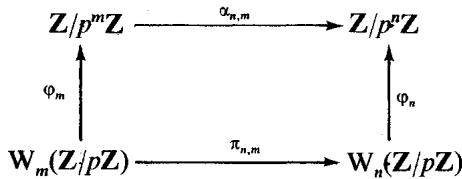
\includegraphics[keepaspectratio]{images/part001_40a15710.jpg}}

is commutative. It follows that \(\varphi = \varprojlim \varphi_n\) is an isomorphism of topological rings from \(\mathbf{W}(\mathbf{Z}/p\mathbf{Z}) = \varprojlim \mathbf{W}_n(\mathbf{Z}/p\mathbf{Z})\) onto \(\mathbf{Z}_p = \varprojlim \mathbf{Z}/p^n\mathbf{Z}\) (III, § 2, no. 12, example 3).

Let \(m\) and \(n\) be two integers \(\geqslant 1\) . By construction, one has an exact sequence of additive groups

\[
0 \longrightarrow \mathrm{W} (\mathrm{A}) \xrightarrow {\mathrm{V} ^ {m}} \mathrm{W} (\mathrm{A}) \xrightarrow {\pi_ {m}} \mathrm{W} _ {m} (\mathrm{A}) \longrightarrow 0.\tag{E}
\]

Passing to quotients, the endomorphism \(V^{n}\) of the additive group of W(A) defines a homomorphism \(V_{m}^{n}\) from the additive group of \(W_{m}(A)\) to that of \(W_{m+n}(A)\) . In other words, one has a commutative diagram

\pandocbounded{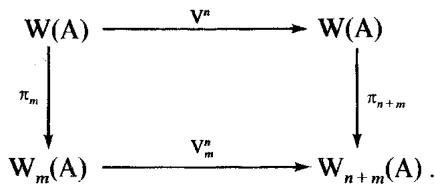
\includegraphics[keepaspectratio]{images/part001_7fe9268c.jpg}}

Passing to quotients, one deduces from the exact sequence (E) an exact sequence

\[
0 \longrightarrow \mathrm{W} _ {m} (\mathrm{A}) \xrightarrow {\mathrm{V} _ {m} ^ {n}} \mathrm{W} _ {n + m} (\mathrm{A}) \xrightarrow {\pi_ {n , n + m}} \mathrm{W} _ {n} (\mathrm{A}) \longrightarrow 0.\tag{E'}
\]

We have

\[
\mathrm{V} _ {m} ^ {n} [ a _ {0}, \dots , a _ {m - 1} ] = [ \underbrace {0 , \dots , 0} _ {n \text {   times }}, a _ {0}, \dots , a _ {m - 1} ],\tag{45}
\]

for every element \([a_0, \ldots, a_{m-1}]\) of \(\mathbf{W}_m(\mathbf{A})\) .

By prop. 3, c) of no. 5, one has FV \(^{m+1}\) (a) = p.V \(^{m}\) (a) for all a in W(A) and we consequently have F(V \(_{m+1}\) (A)) ⊂ V \(_{m}\) (A). By induction on n, it follows that F \(^{n}\) maps V \(_{n+m}\) (A) into V \(_{m}\) (A), and therefore defines, by passing to quotients, a ring homomorphism F \(^{n}\) :W \(_{n+m}\) (A) → W \(_{m}\) (A). By construction, we have a commutative diagram

\pandocbounded{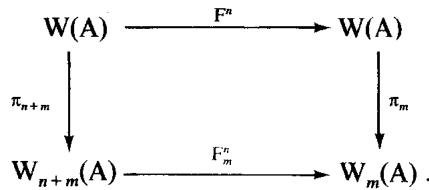
\includegraphics[keepaspectratio]{images/part001_14e9ec0a.jpg}}

Recall (no. 3) that the polynomial \(\mathbf{F}_i\) belongs to \(\mathbf{Z}[\mathbf{X}_0, \ldots, \mathbf{X}_{i+1}]\) for every integer \(i \geqslant 0\) ; the homomorphism \(\mathbf{F}_m^1\) from \(\mathbf{W}_{m+1}(\mathbf{A})\) to \(\mathbf{W}_m(\mathbf{A})\) is therefore made explicit as follows:

\[
\mathrm{F} _ {m} ^ {1} \left[ a _ {0}, \dots , a _ {m} \right] = \left[ \mathrm{F} _ {i} \left(a _ {0}, \dots , a _ {i + 1}\right) \right] _ {0 \leqslant i <   m}.\tag{46}
\]

Let \(\boldsymbol{a} \in \mathrm{W}_{m}(\mathbf{A})\) , \(\boldsymbol{a}' \in \mathrm{W}_{m}(\mathbf{A})\) and \(\boldsymbol{b} \in \mathrm{W}_{m+1}(\mathbf{A})\). The following formulas result by passing to quotients from Prop. 3 of No. 5:

\begin{enumerate}
\def\labelenumi{(\arabic{enumi})}
\setcounter{enumi}{46}
\tightlist
\item
\end{enumerate}

\[
\mathrm{F} _ {m} ^ {1} \left(\mathrm{V} _ {m} ^ {1} (\boldsymbol {a})\right) = p. \boldsymbol {a}\tag{48}
\]

\[
\mathrm{V} _ {m} ^ {1} (a \times \mathrm{F} _ {m} ^ {1} (b)) = \mathrm{V} _ {m} ^ {1} (a) \times b\tag{49}
\]

\[
\mathrm{V} _ {m} ^ {1} (a) \times \mathrm{V} _ {m} ^ {1} (a ^ {\prime}) = p. \mathrm{V} _ {m} ^ {1} (a \times a ^ {\prime})\tag{50}
\]

\[
\mathrm{V} _ {m} ^ {1} (\mathrm{F} _ {m} ^ {1} (b)) = \mu_ {m + 1} \times b
\]

\((\text{with } \boldsymbol{\mu}_{m+1} = [0, 1, 0, ..., 0]).\)

\subsection{The ring of Witt vectors with coefficients in a ring of characteristic p}

PROPOSITION 5. --- Let A be a ring of characteristic p (A, V, p. 2). For any elements a and b of W(A), and positive integers m and n, if \(\boldsymbol{a} = (a_{n})_{n \in \mathbb{N}}\) ,

\begin{enumerate}
\def\labelenumi{(\arabic{enumi})}
\setcounter{enumi}{50}
\tightlist
\item
\end{enumerate}

\[
\mathrm{F} (\boldsymbol {a}) = (a _ {n} ^ {p}) _ {n \in \mathbf {N}}\tag{52}
\]

\[
p. \boldsymbol {a} = \operatorname{VF} (\boldsymbol {a}) = \operatorname{FV} (\boldsymbol {a}) = (0, a _ {0} ^ {p}, a _ {1} ^ {p}, \dots)\tag{53}
\]

\[
\mathrm{V} ^ {m} (a) \times \mathrm{V} ^ {n} (b) = \mathrm{V} ^ {m + n} (\mathrm{F} ^ {n} (a) \times \mathrm{F} ^ {m} (b)).
\]

Formula (51) follows from Example 4 of No. 3. From this we immediately deduce the equality

\[
\operatorname{VF} (\boldsymbol {a}) = \operatorname{FV} (\boldsymbol {a}) = (0, a _ {0} ^ {p}, a _ {1} ^ {p}, \dots),
\]

and the equality \(p\) . \(a = \text{FV}(a)\) was proved (no. 5, prop. 3), whence (52).

Let us prove (53). By formula (37) (where we substitute \(V^n(\boldsymbol{b})\) for \(\boldsymbol{b}\) ), we have

\[
\mathrm{V} ^ {m} (\boldsymbol {a}) \times \mathrm{V} ^ {n} (\boldsymbol {b}) = \mathrm{V} ^ {m} \left(\boldsymbol {a} \times \mathrm{F} ^ {m} \left(\mathrm{V} ^ {n} (\boldsymbol {b})\right)\right).\tag{54}
\]

From formula (37), we also deduce

\[
\mathrm{V} ^ {n} \left(\mathrm{F} ^ {m} (\boldsymbol {b})\right) \times \boldsymbol {a} = \mathrm{V} ^ {n} \left(\mathrm{F} ^ {m} (\boldsymbol {b}) \times \mathrm{F} ^ {n} (\boldsymbol {a})\right).\tag{55}
\]

Formula (53) then follows from (54) and (55) and the relation \(F^{m} \circ V^{n} = V^{n} \circ F^{m}\) , itself a consequence of (51).

COROLLARY. --- If m and n are two positive integers, we have

\[
\mathrm{V} _ {m} (\mathrm{A}) \times \mathrm{V} _ {n} (\mathrm{A}) \subset \mathrm{V} _ {m + n} (\mathrm{A}).
\]

This follows from formula (53), since \(V_{m}(A)\) is the image of \(V^{m}:W(A)\to W(A)\) .

PROPOSITION 6.---Let A be a ring.

\begin{enumerate}
\def\labelenumi{\alph{enumi})}
\item
  For every integer \(k \geqslant 1\) , one has \((\mathrm{V}_1(\mathrm{A}))^k = p^{k-1} \cdot \mathrm{V}_1(\mathrm{A})\) .
\item
  Suppose that A is a ring of characteristic p. On the ring W(A), the V₁(A)-adic topology and the p-adic topology coincide, and they are finer than the product topology ℰ (cf. no. 6). The ring W(A) is separated and complete for the p-adic topology.
\end{enumerate}

Let us prove \(a\) ) by induction on \(k\) . The case \(k = 1\) is evident. Suppose \(k \geqslant 2\) . By the induction hypothesis, we have \(\mathrm{V}_{1}(\mathrm{A})^{k-1} = p^{k-2} \cdot \mathrm{V}_{1}(\mathrm{A})\) and consequently \(\mathrm{V}_{1}(\mathrm{A})^{k} = p^{k-2} \cdot (\mathrm{V}_{1}(\mathrm{A}))^{2}\) . But it follows from prop. 3, \(d\) ), formula (31), of no. 5 that one has \((\mathrm{V}_{1}(\mathrm{A}))^{2} = p \cdot \mathrm{V}_{1}(\mathrm{A})\) , whence \(a\) ).

Suppose now that A has characteristic p. Since one has

\[
p. \mathrm{W} (\mathrm{A}) = \mathrm{VF} (\mathrm{W} (\mathrm{A})) \subset \mathrm{V} _ {1} (\mathrm{A}) \quad (\text { formula (52) }),
\]

one deduces from \(a\) ) the inclusions \(p^{k} \cdot \mathbf{W}(\mathbf{A}) \subset (\mathbf{V}_{1}(\mathbf{A}))^{k} \subset p^{k-1} \cdot \mathbf{W}(\mathbf{A})\) , and from the corollary to prop. 5 the inclusion \((\mathbf{V}_{1}(\mathbf{A}))^{k} \subset \mathbf{V}_{k}(\mathbf{A})\) , for every integer \(k \geqslant 1\) . The first assertion of \(b\) ) follows from this.

Let \(k\) be an integer \(\geqslant 1\) . By formula (52), the ideal \(p^{k}\) . W(A) of W(A) is the set of elements \(\boldsymbol{a} = (a_{n})_{n \in \mathbf{N}}\) of W(A) such that one has \(a_{n} = 0\) for \(n < k\) and \(a_{n} \in A^{p^{k}}\) for \(n \geqslant k\) . It is therefore closed for the topology \(\mathcal{G}\) . Since W(A) is separated and complete for the topology \(\mathcal{G}\) and the ideals \(p^{k}\) . W(A) of W(A), for \(k \geqslant 1\) , form a neighborhood base of 0 in W(A) for the \(p\)-adic topology, the ring W(A) is separated and complete for the \(p\)-adic topology (TG, III, p. 26, cor. 1 to prop. 10).

PROPOSITION 7. --- Let A be a perfect ring of characteristic p.

\begin{enumerate}
\def\labelenumi{\alph{enumi})}
\item
  For every element \(\boldsymbol{a} = (a_{n})_{n \in \mathbb{N}}\) of W(A), the series with general term \(p^{n}\tau(a_{n}^{p^{-n}})\) is convergent in W(A), with sum a.
\item
  On \(\mathbf{W}(\mathbf{A})\) , the \(\mathbf{V}_1(\mathbf{A})\)-adic topology, the \(p\)-adic topology and the topology \(\mathcal{C}\) coincide. More precisely, we have \(\mathbf{V}_n(\mathbf{A}) = p^n\) . \(\mathbf{W}(\mathbf{A}) = (\mathbf{V}_1(\mathbf{A}))^n\) for every integer \(n \geqslant 0\) . In particular \(\Phi_0\) defines an isomorphism from \(\mathbf{W}(\mathbf{A})/p\) . \(\mathbf{W}(\mathbf{A})\) onto \(\mathbf{A}\) .
\end{enumerate}

By definition (A, V, p. 5), the map \(a \mapsto a^{p}\) is an automorphism of the ring A. By prop. 5, F is therefore an automorphism of the ring W(A), and one has, for every \(n \in \mathbf{N}\) ,

\[
p ^ {n}. \mathrm{W} (\mathrm{A}) = \mathrm{V} ^ {n} \mathrm{F} ^ {n} (\mathrm{W} (\mathrm{A})) = \mathrm{V} ^ {n} (\mathrm{W} (\mathrm{A})) = \mathrm{V} _ {n} (\mathrm{A}).
\]

In particular, we have \((\mathbf{V}_1(\mathbf{A}))^n = (p.\mathbf{W}(\mathbf{A}))^n = p^n.\mathbf{W}(\mathbf{A})\) . The assertion \(b)\) follows from that. By prop. 5, we have

\[
p ^ {n} \cdot \tau (a _ {n} ^ {p ^ {- n}}) = \mathrm{V} ^ {n} \mathrm{F} ^ {n} \tau (a _ {n} ^ {p ^ {- n}}) = \mathrm{V} ^ {n} \tau (a _ {n}),
\]

and assertion a) follows from prop. 4 of no. 6.

PROPOSITION 8. — Let A be a field of characteristic p. The ring W(A) is a local integral domain, separated and complete, with maximal ideal V₁(A) and residue field isomorphic to A. If the field A is perfect, the ring W(A) is a discrete valuation ring, and its maximal ideal is p.W(A).

The homomorphism \(\Phi_{0}\) defines an isomorphism from W(A)/V \(_{1}\) (A) onto A (no. 7, example 1). The ideal V \(_{1}\) (A) of W(A) is therefore maximal. Since the ring W(A) is separated and complete for the topology V \(_{1}\) (A)-adic (prop. 6, b)), it is a local ring, with maximal ideal V \(_{1}\) (A) (III, § 2, no. 13, prop. 19).

Let \(\pmb{a}\) and \(\pmb{b}\) be two nonzero elements of \(\mathbf{W}(\mathbf{A})\) . There exist integers \(m \geqslant 0\) and \(n \geqslant 0\) , and elements \(\pmb{a}' = (a_n')_{n \in \mathbb{N}}\) and \(\pmb{b}' = (b_n')_{n \in \mathbb{N}}\) of \(\mathbf{W}(\mathbf{A})\) such that \(\pmb{a} = \mathbf{V}^m(\pmb{a}')\) , \(\pmb{b} = \mathbf{V}^n(\pmb{b}')\) and such that the elements \(a_0'\) and \(b_0'\) of \(\mathbf{A}\) are nonzero. Then the component of index \(m + n\) of \(\pmb{a} \times \pmb{b}\) is equal to the component of index 0 of \(\mathbf{F}^n(\pmb{a}') \times \mathbf{F}^m(\pmb{b}')\) (formula (53)), that is, to \(a_0'^{p^n} b_0'^{p^m}\) (formula (51) and no. 3, example 2). Consequently \(\pmb{a} \times \pmb{b}\) is nonzero and \(\mathbf{W}(\mathbf{A})\) is integral.

If the field A is perfect, the maximal ideal \(V_{1}(A)\) of \(W(A)\) is equal to p.\(W(A)\)

(prop. 7, b)) and consequently W(A) is a discrete valuation ring (VI, § 3, no. 6, prop. 9, c)).

Remarks. --- 1) Let A be a field of characteristic p. One can show that the ring W(A) is Noetherian if and only if A is perfect (p. 43, exerc. 9).

\begin{enumerate}
\def\labelenumi{\arabic{enumi})}
\setcounter{enumi}{1}
\tightlist
\item
  Let A be a ring of characteristic p. By prop. 5, we have the formulas
\end{enumerate}

\[
\mathrm{F} _ {m} ^ {n} [ a _ {0}, \dots , a _ {n + m - 1} ] = [ a _ {0} ^ {p ^ {n}}, \dots , a _ {m - 1} ^ {p ^ {n}} ]
\]

\[
p ^ {n} \cdot [ a _ {0}, \dots , a _ {n + m - 1} ] = [ \underbrace {0 , \dots , 0} _ {n \text {   times }}, a _ {0} ^ {p ^ {n}}, \dots , a _ {m - 1} ^ {p ^ {n}} ]
\]

for every Witt vector \([a_0, \dots, a_{n+m-1}]\) of length \(n + m\) .

In fact, the map \(F:W(A)\to W(A)\) allows one, by passing to quotients by \(V_{m}(A)\) , to define a map \(\overline{F}_{m}:W_{m}(A)\to W_{m}(A)\) . We have the formula

\[
\overline {{{{\mathrm{F}}}}} _ {m} \left[ a _ {0}, \dots , a _ {m - 1} \right] = \left[ a _ {0} ^ {p}, \dots , a _ {m - 1} ^ {p} \right].
\]

The maps \(V_{m}^{1} \circ \overline{F}_{m}\) and \(\overline{F}_{m+1} \circ V_{m}^{1}\) from \(W_{m}(A)\) to \(W_{m+1}(A)\) are equal and are deduced, by passing to the quotient, from multiplication by p in \(W_{m+1}(A)\) .

\section{COHEN RINGS}

Throughout this section, p denotes a prime number.

\subsection{\texorpdfstring{\(p\) -rings}{p-rings}}

DEFINITION 1. --- A ring C is said to be a p-ring if the ideal pC of C is maximal, and if C is separated and complete for the pC-adic topology.

Let C be a ring; if \(p1_{C}\) is nilpotent and if the ideal pC of C is maximal, C is a p-ring, for the pC-adic topology of C is discrete. In particular, every field of characteristic p is a p-ring.

PROPOSITION 1. --- Let C be a p-ring.

\begin{enumerate}
\def\labelenumi{\alph{enumi})}
\item
  The ring C is local, with maximal ideal pC.
\item
  Suppose that \(p1_{\mathbb{C}}\) is nilpotent. Let \(d\) be the smallest positive integer such that \(p^{d}1_{\mathbb{C}} = 0\) . The ideals of \(\mathbb{C}\) are of the form \(p^{k}\mathbb{C}\) with \(0 \leqslant k \leqslant d\) and one has \(p^{k}\mathbb{C} \neq p^{l}\mathbb{C}\) when \(k\) and \(l\) are two distinct integers satisfying \(0 \leqslant k \leqslant d, 0 \leqslant l \leqslant d\) . The \(\mathbb{C}\) -module \(\mathbb{C}\) is of length \(d\) .
\item
  Suppose that \(p1_{\mathbb{C}}\) is not nilpotent. Then C is a discrete valuation ring whose residue field is of characteristic \(p\) , and whose field of fractions is of characteristic 0. The ideals of the form \(p^{n}\mathbf{C}\) , with \(n \in \mathbf{N}\) , are pairwise distinct; they form all the nonzero ideals of C. The C-module C is not of finite length.
\end{enumerate}

The assertion \(a)\) follows from prop. 19 of III, § 2, no. 13.

We have \(\bigcap_{n\geqslant 0}p^{n}\mathbf{C} = \{0\}\) by hypothesis. Let \(x\neq 0\) in \(\mathbf{C}\) ; there exists an integer \(n\geqslant 0\) such that \(x\in p^n\mathbf{C}, x\notin p^{n + 1}\mathbf{C}\) ; there therefore exists an element \(y\) of \(\mathbf{C}\) such that \(x = p^n y\) ; since \(y\) does not belong to \(p\mathbf{C}\) , \(y\) is invertible.

Suppose that \(p1_{\mathbb{C}}\) is not nilpotent. If \(x\) and \(x'\) are two nonzero elements of C, there exist two integers \(n \geqslant 0\) , \(n' \geqslant 0\) and two invertible elements \(y\) , \(y'\) of C such that \(x = p^n y\) , \(x' = p^{n'} y'\) . Then one has \(xx' = p^{n+n'} yy' \neq 0\) , hence C is an integral domain. Since C is a local ring, but is not a field, and the maximal ideal \(m_{\mathbb{C}} = p\mathbb{C}\) of C is principal, C is a discrete valuation ring (VI, § 3, no. 6, prop. 9). The nonzero ideals of C are then of the form \(p^n\mathbb{C}\) by loc. cit., prop. 8, and are pairwise distinct. In particular, the ring C is not Artinian, hence the C-module C is not of finite length. The residue field C/pC of C is of characteristic \(p\) . Let \(q\) be the characteristic of the field of fractions of C. We have \(p1_{\mathbb{C}} \neq 0\) , whence \(p \neq q\) . Moreover, if \(q\) were nonzero, we would have \(q1_{\mathbb{C}} = 0\) , hence C/pC would be of characteristic \(q \neq p\) , which is absurd. This proves \(c\) ).

Suppose that \(p1_{C}\) is nilpotent. Let \(d\) be the smallest positive integer such that \(p^{d}1_{C} = 0\) . We have a sequence of ideals

\[
\mathrm{C} \supset p \mathrm{C} \supset p ^ {2} \mathrm{C} \supset \dots \supset p ^ {d - 1} \mathrm{C} \supset p ^ {d} \mathrm{C} = \{0 \}.\tag{E}
\]

If \(k\) is an integer such that \(0 \leqslant k < d\) and \(p^k\mathbf{C} = p^{k+1}\mathbf{C}\) , then we deduce

\[
p ^ {d - k - 1} p ^ {k} \mathrm{C} = p ^ {d - k - 1} p ^ {k + 1} \mathrm{C} = \{0 \}
\]

contrary to the hypothesis \(p^{d-1}1_{\mathbf{C}} \neq 0\) . Hence the elements of the sequence (E) are pairwise distinct. Let \(\mathfrak{a}\) be an ideal of C and let \(k\) be the smallest positive integer such that \(\mathfrak{a} \supset p^k\mathbf{C}\) . Let \(x\) be a nonzero element of \(\mathfrak{a}\) ; we have seen that \(x\) is of the form \(p^m u\) with \(m \geqslant 0\) and \(u\) is invertible in C. We therefore have \(p^m\mathbf{C} \subset \mathfrak{a}\) , whence \(m \geqslant k\) , and finally \(x \in p^k\mathbf{C}\) . In conclusion, we have \(\mathfrak{a} = p^k\mathbf{C}\) . The sequence (E) is then a Jordan-Hölder sequence of the C-module C, which is of length \(d\) .

COROLLARY 1. --- If the p-ring C is an integral domain, it is a discrete valuation ring, or a field of characteristic p.

Suppose C is integral. If \(p1_{\mathbf{C}}\) is nilpotent, we have \(p1_{\mathbf{C}} = 0\) , and \(\{0\}\) is a maximal ideal of C, hence C is a field of characteristic \(p\) . If \(p1_{\mathbf{C}}\) is not nilpotent, then C is a discrete valuation ring by prop. 1, c).

COROLLARY 2. --- Let C be a p-ring and a an ideal of C distinct from C. The ring C/a is a p-ring.

We may assume \(\mathfrak{a} \neq \{0\}\) . There then exists an integer \(i \geqslant 1\) such that \(\mathfrak{a} = p^i\mathrm{C}\) ; the ideal \(p\mathrm{C} / \mathfrak{a}\) of \(\mathrm{C} / \mathfrak{a}\) is maximal and we have \(p^i1_{\mathrm{C} / \mathfrak{a}} = 0\) , hence \(\mathrm{C} / \mathfrak{a}\) is a \(p\) -ring.

Let C be a \(p\) -ring. We call the length of C, and denote by \(l(\mathbf{C})\) , the least upper bound in \(\overline{\mathbf{R}}\) of the set of integers \(n \geqslant 1\) such that \(p^{n-1}1_{\mathbf{C}} \neq 0\) . When \(l(\mathbf{C})\) is finite, it is the length of the C-module C, and when \(l(\mathbf{C})\) is equal to \(+\infty\) , the C-module C is not of finite length (prop. 1).

Examples. --- 1) For every integer \(n \geqslant 1\) , the ring \(\mathbf{Z}/p^{n}\mathbf{Z}\) is a \(p\) -ring of length \(n\) . The ring \(\mathbf{Z}_{p}\) of \(p\) -adic integers is a \(p\) -ring of infinite length.

\begin{enumerate}
\def\labelenumi{\arabic{enumi})}
\setcounter{enumi}{1}
\tightlist
\item
  Let K be a perfect field of characteristic p. By prop. 8 of § 1, no. 8, the ring W(K) of Witt vectors is a p-ring of infinite length. The map \((a_{n})_{n\in\mathbf{N}} \mapsto a_{0}\) induces by passage to the quotient an isomorphism of W(K)/pW(K) onto the field K (loc. cit., prop. 7). For every integer \(n \geqslant 1\) , the ring
\end{enumerate}

\[
\mathrm{W} _ {n} (\mathrm{K}) = \mathrm{W} (\mathrm{K}) / p ^ {n} \mathrm{W} (\mathrm{K})
\]

is a p-ring of length n.

PROPOSITION 2. --- Let C and C' be two p-rings and let \(u\) be a homomorphism from C to C'. Let \(v\) be the homomorphism from \(\kappa_{\mathbf{C}} = \mathbf{C} / p\mathbf{C}\) to \(\kappa_{\mathbf{C}'} = \mathbf{C}' / p\mathbf{C}'\) induced by u by passage to the quotients.

\begin{enumerate}
\def\labelenumi{\alph{enumi})}
\item
  We have \(l(\mathbf{C}) \geqslant l(\mathbf{C}')\) and u is injective if and only if \(l(\mathbf{C}) = l(\mathbf{C}')\) .
\item
  For u to be surjective, it is necessary and sufficient that v be an isomorphism.
\item
  For u to be an isomorphism, it is necessary and sufficient that v be an isomorphism and that we have \(l(\mathbf{C}) = l(\mathbf{C}')\) .
\end{enumerate}

Let \(n \geqslant 1\) be an integer. One has \(u(p^{n-1}1_{\mathbf{C}}) = p^{n-1}1_{\mathbf{C}'}\) , hence the relation \(p^{n-1}1_{\mathbf{C}'} \neq 0\) implies \(p^{n-1}1_{\mathbf{C}} \neq 0\) and is equivalent to it if \(u\) is injective. We therefore have \(l(\mathbf{C}') \leqslant l(\mathbf{C})\) with equality if \(u\) is injective. If \(u\) is not injective, there exists an integer \(i < l(\mathbf{C})\) such that the kernel of \(u\) is the ideal \(p^i\mathbf{C}\) of \(\mathbf{C}\) ; we then have \(p^i1_{\mathbf{C}'} = 0\) , whence \(l(\mathbf{C}') \leqslant i\) . This proves \(a\) ).

Since \(\kappa_{\mathrm{C}}\) and \(\kappa_{\mathrm{C}'}\) are fields, the homomorphism \(v\) is injective. If \(u\) is surjective, so is \(v\) , which is therefore an isomorphism. Conversely, suppose \(v\) is surjective. Then for every integer \(n \geqslant 0\) , the map \(v_{n}: p^{n}\mathrm{C}/p^{n+1}\mathrm{C} \to p^{n}\mathrm{C}'/p^{n+1}\mathrm{C}'\) derived from \(u\) is surjective. Since C is complete for the \(p\mathrm{C}\)-adic filtration and \(\mathbf{C}'\) separated for the \(p\mathbf{C}'\)-adic filtration, \(u\) is surjective by Cor. 2 of Th. 1 of III, § 2, No. 8. This proves \(b\) ).

Finally, c) follows from a) and b).

PROPOSITION 3. --- Let \((\mathbf{C}_{n}, \pi_{n,m})\) be a projective system of rings relative to the index set N. We assume that \(\mathbf{C}_{n}\) is a p-ring for all \(n \in \mathbf{N}\) and that the homomorphisms \(\pi_{n,m}\) are surjective. Then \(C = \varprojlim C_{n}\) is a p-ring, and for all \(n \in \mathbf{N}\) the canonical homomorphism \(\pi_{n}: C \to C_{n}\) is surjective and induces an isomorphism of \(\kappa_{C}\) onto \(\kappa_{C_{n}}\) .

As the maps \(\pi_{n,m}\) are surjective, the same holds for the maps \(\pi_n\) (E, III, p. 58, prop. 5). Let us show that C is a \(p\) -ring. Let \(d_n\) be the length of \(\mathbf{C}_n\) . By prop. 2, a), the sequence of elements \(d_n\) of \(\mathbf{N} \cup \{+\infty\}\) is increasing; if it is stationary, there exists an integer \(n_0\) such that \(\pi_{n,m}\) is an isomorphism of \(\mathbf{C}_m\) onto \(\mathbf{C}_n\) when \(n_0 \leqslant n \leqslant m\) , so that C, which is isomorphic to \(\mathbf{C}_{n_0}\) , is a \(p\) -ring.

It therefore suffices to consider the case where each \(d_{n}\) is finite, and where the sequence \((d_{n})\) tends to \(+\infty\) . Endow the ring C with the trivial filtration (III, § 2, n° 1, example 5). For \(n\in\mathbf{N}\) , let \(\mathbf{I}_{n}\) be the kernel of \(\pi_{n}\) ; set \(\mathbf{I}_{n}=\mathbf{C}\) if \(n<0\) . Let E denote the C-module C equipped with the filtration \((\mathbf{I}_{n})_{n\in\mathbf{Z}}\) . It is separated and complete, because the topology \(\mathcal{G}\) defined by the filtration \((\mathbf{I}_{n})_{n\in\mathbf{Z}}\) is the projective limit topology of the discrete topologies on the \(\mathbf{C}_{n}\) .

Let \(k\) be an integer \(\geqslant 1\) . We have \(p^{k}\mathrm{C} \subset \varprojlim (p^{k}\mathrm{C}_{n})\) (E, III, p. 55, formula (9)). Conversely, if \(x = (x_{n})_{n \in \mathbb{N}} \in \varprojlim (p^{k}\mathrm{C}_{n})\) and if one sets \(\mathrm{X}_{n} = \{y \in \mathrm{C}|\pi_{n}(p^{k}y) = x_{n}\}\) , the sequence \((\mathrm{X}_{n})_{n \in \mathbb{N}}\) is a decreasing sequence of nonempty closed affine subsets of E. Since \(\mathrm{E / I}_{n}\) is an artinian C-module, the intersection of the \(\mathrm{X}_{n}\) is nonempty (III, § 2, n° 7, prop. 7); for every \(z \in \bigcap_{n \in \mathbb{N}} \mathrm{X}_{n}\) we have \(p^{k}z = x\) . We have therefore proved that one has \(p^{k}\mathrm{C} = \varprojlim p^{k}\mathrm{C}_{n}\) .

for every integer \(k \geqslant 1\) . In particular, the ideal \(p^{k}\text{C}\) of C is closed for the topology \(\mathcal{G}\) . On C, the \(p\) -adic topology is finer than the topology \(\mathcal{G}\) because one has \(p^{d_{n}}\text{C} \subset \text{I}_{n}\) . It then follows from TG, III, p. 26, cor. 1 to prop. 10, that C is separated and complete for the \(p\text{C}\) -adic topology. Moreover, one has \(p\text{C} = \varprojlim p\text{C}_{n} = \pi_{0}^{-1}(p\text{C}_{0})\) and hence the surjective homomorphism of C/pC into \(\text{C}_{0}/p\text{C}_{0}\) deduced from \(\pi_{0}\) is an isomorphism. This shows that the ideal \(p\text{C}\) of C is maximal and consequently that C is a \(p\) -ring. The last assertion of prop. 3 follows from prop. 2, b).

\subsection{Cohen rings}

DEFINITION 2. --- Let A be a separated and complete local ring, whose residue field is of characteristic p. One calls a Cohen subring of A a subring C of A which is a p-ring such that \(\mathbf{A} = \mathfrak{m}_{\mathbf{A}} + \mathbf{C}\) (i.e. \(\mathbf{A}/\mathfrak{m}_{\mathbf{A}} = \mathbf{C}/(\mathfrak{m}_{\mathbf{A}} \cap \mathbf{C})\) ).

If C is a Cohen subring of A, the ideal \(m_{A} \cap C\) of C is maximal, hence equal to pC. The canonical map from \(\kappa_{C} = C/pC\) onto \(\kappa_{A} = A/m_{A}\) is therefore an isomorphism of fields.

Example. --- Let C be a p-ring. The ring of formal power series \(A = C[[T_{1}, \ldots, T_{n}]]\) is a Noetherian local ring, separated and complete, whose maximal ideal is generated by the sequence (p, T₁, \ldots, Tₙ). It is immediate that C is a Cohen subring of A. This applies in particular when C is equal to Zₚ, to Z/pⁿZ, or to a field of characteristic p.

THEOREM 1. — Let A be a local ring, separated and complete, whose residue field k has characteristic p. Let π be the canonical map from A onto k, and let S be a subset of A such that π induces a bijection from S onto a p-basis of k (A, V, p. 95).

\begin{enumerate}
\def\labelenumi{\alph{enumi})}
\item
  There exists a Cohen subring C of A containing S, and it is unique.
\item
  The subring C of A is closed, and the \(p\)C-adic topology on C is induced by the \(m_{A}\)-adic topology of A.
\item
  Every closed subring A' of A, containing S, and such that \(A = A' + m_{A}\) contains C.
\end{enumerate}

\begin{enumerate}
\def\labelenumi{\Alph{enumi})}
\tightlist
\item
  Special case: \(\mathfrak{m}_{\mathbf{A}}\) nilpotent
\end{enumerate}

Let \(n\) be a positive integer such that \(\mathfrak{m}_{\mathbf{A}}^{n+1}=\{0\}\) . If \(\Phi_{n}\) is the \(n\) -th Witt polynomial ( § 1, no. 1 ), the map \(u:[a_{0},..., a_{n}]\mapsto\Phi_{n}(a_{0},..., a_{n})\) is a ring homomorphism from \(\mathbf{W}_{n+1}(\mathbf{A})\) to \(\mathbf{A}\) ( § 1, no. 7 ). Let \(\mathbf{B}_{n}\) be the image of \(u\) and let \(\mathbf{C}_{n}\) be the subring of \(\mathbf{A}\) generated by \(\mathbf{B}_{n}\cup\mathbf{S}\) .

Lemma 1. --- Let A' be a subring of A containing S. For A' to contain \(\mathbf{C}_{n}\) , it is necessary and sufficient that \(A' + m_{A} = A\).

We have \(pA \subset m_A\) and \(B_n\) consists of the elements of the form \(a_0^{p^n} + pa_1^{p^{n-1}} + \cdots + p^n a_n\) with \(a_0, \ldots, a_n\) in A. Consequently, we have \(\pi(B_n) = k^{p^n}\) , whence \(\pi(C_n) = k^{p^n}[\pi(S)]\) . But since \(\pi(S)\) is a \(p\) -basis of \(k\) , one has \(k = k^{p^n}[\pi(S)]\) (A, V, p. 96), whence \(\pi(C_n) = k\) , that is, \(C_n + m_A = A\) .

Let A' be a subring of A containing S. If A' contains \(C_{n}\) , one has

\[
\mathrm{A} ^ {\prime} + \mathrm{m} _ {\mathrm{A}} \supset \mathrm{C} _ {n} + \mathrm{m} _ {\mathrm{A}} = \mathrm{A}, \quad \mathrm{whence} \quad \mathrm{A} ^ {\prime} + \mathrm{m} _ {\mathrm{A}} = \mathrm{A}.
\]

Conversely, suppose we have \(\mathbf{A}' + \mathfrak{m}_{\mathbf{A}} = \mathbf{A}\) . Let \(a_0, \ldots, a_n\) be elements of \(\mathbf{A}\) ; by hypothesis there exist elements \(a_0', \ldots, a_n'\) of \(\mathbf{A}'\) such that \(a_i \equiv a_i'\) mod. \(\mathfrak{m}_{\mathbf{A}}\) for \(0 \leqslant i \leqslant n\) . By prop. 1 of § 1, no. 1 and the hypothesis \(\mathfrak{m}_{\mathbf{A}}^{n+1} = \{0\}\) , one therefore has \(\Phi_n(a_0, \ldots, a_n) = \Phi_n(a_0', \ldots, a_n') \in \mathbf{A}'\) , whence \(\mathbf{B}_n \subset \mathbf{A}'\) . Since \(\mathbf{C}_n\) is the ring generated by \(\mathbf{B}_n \cup \mathbf{S}\) , one has \(\mathbf{C}_n \subset \mathbf{A}'\) .

In the set S of subrings A' of A containing S and such that \(A' + m_{A} = A\) there exists, by lemma 1, a smallest element C, and one has \(C_{n} = C\) for every integer \(n \geqslant 0\) such that \(m_{A}^{n+1} = \{0\}\) .

We have \(C + m_A = A\) by construction and \(p1_C\) is nilpotent. One obviously has \(pC \subset C \cap m_A\) and lemma 2 below therefore shows that \(pC\) is a maximal ideal of \(C\) and consequently that \(C\) is a Cohen subring of \(A\) .

Lemma 2. --- One has \(C \cap m_{A} \subset pC\).

Let us choose an integer \(m \geqslant 1\) such that \(\mathfrak{m}_{\mathbf{A}}^{m} = \{0\}\) , whence \(\mathbf{C} = \mathbf{C}_{m} = \mathbf{C}_{m-1}\) . Let \(\Lambda\) be the part of \(\mathbf{N}^{(\mathbf{S})}\) consisting of families with finite support of integers \((\alpha_{s})_{s \in \mathbf{S}}\) satisfying \(0 \leqslant \alpha_{s} < p^{m}\) for every \(s \in \mathbf{S}\) . Since \(\mathbf{B}_{m}\) contains \(s^{p^{m}} = \Phi_{m}(s, 0, ..., 0)\) for every \(s \in \mathbf{S}\) , the monomials \(Z_{\alpha} = \prod_{s \in \mathbf{S}} s^{\alpha_{s}}\) , where \(\alpha\) ranges over \(\Lambda\) , generate \(\mathbf{C}_{m}\) as a \(\mathbf{B}_{m}\) -module. Moreover, by the formula

\[
\Phi_ {m} (a _ {0}, \dots , a _ {m}) = a _ {0} ^ {p ^ {m}} + p \Phi_ {m - 1} (a _ {1}, \dots , a _ {m}),
\]

every element of \(B_{m}\) is of the form \(a^{p^{m}} + pb\) with \(a \in A\) and \(b \in B_{m-1}\) . Consequently every element of \(C = C_{m}\) is of the form

\[
x = \sum_ {\alpha \in \Lambda} c _ {\alpha} ^ {p ^ {m}} Z _ {\alpha} + p y\tag{1}
\]

with \(c_{\alpha} \in \mathbf{A}\) for every \(\alpha \in \Lambda\) , and \(y \in \mathbf{C}_{m-1} = \mathbf{C}\) . If \(x\) belongs to \(\mathbf{C} \cap \mathfrak{m}_{\mathbf{A}}\) , one has \(\pi(x) = 0\) , whence \(\sum_{\alpha \in \Lambda} \pi(c_{\alpha})^{p^m} \pi(Z_{\alpha}) = 0\) . Since \(\pi(\mathbf{S})\) is a \(p\) -basis of \(k\) , one has \(\pi(c_{\alpha}) = 0\) for every \(\alpha \in \Lambda\) according to A, V, p. 96. We then have \(c_{\alpha} \in \mathfrak{m}_{\mathbf{A}}\) , whence \(c_{\alpha}^m = 0\) and a fortiori \(c_{\alpha}^{p^m} = 0\) . By (1), we have \(x = py\) , whence lemma 2.

We have \(p^m\mathbf{C} = \mathfrak{m}_{\mathbf{A}}^m = \{0\}\) for \(m\) sufficiently large, and assertion \(b)\) is therefore trivial. Assertion \(c)\) follows from lemma 1. If \(\mathbf{C}'\) is a Cohen subring of A containing S, we have \(\mathbf{C}' \supset \mathbf{C}\) by lemma 1. But since the inclusion of C in \(\mathbf{C}'\) induces an isomorphism of \(\kappa_{\mathbf{C}}\) onto \(\kappa_{\mathbf{C}'}\) , one has \(\mathbf{C} = \mathbf{C}'\) (no. 1, prop. 2, b)), and this completes the proof of \(a\) ).

\noindent\textbf{B) General case.}\par

For every integer \(n \geqslant 0\) , denote by \(\mathbf{A}_n\) the local ring \(\mathbf{A}/\mathfrak{m}_{\mathbf{A}}^{n+1}\) , \(\mathfrak{m}_n = \mathfrak{m}_{\mathbf{A}}/\mathfrak{m}_{\mathbf{A}}^{n+1}\) its maximal ideal, and \(\pi_n\) the canonical homomorphism from A onto \(\mathbf{A}_n\) . By A), there exists a unique Cohen subring \(\mathbf{C}_n\) of \(\mathbf{A}_n\) containing \(\pi_n(\mathbf{S})\) . When \(0 \leqslant n \leqslant m\) , denote by \(\pi_{n,m}\) the canonical homomorphism from \(\mathbf{A}_m\) onto \(\mathbf{A}_n\) . By cor. 2 of prop. 1 of no. 1, \(\pi_{n,m}(\mathbf{C}_m)\) is a \(p\) -ring; we have \(\pi_{n,m}(\mathbf{C}_m) + \mathfrak{m}_n = \mathbf{A}_n\) , hence \(\pi_{n,m}(\mathbf{C}_m)\) is equal to the Cohen subring \(\mathbf{C}_n\) of \(\mathbf{A}_n\) . By prop. 3 of no. 1, the subring \(\varprojlim \mathbf{C}_n\) of \(\varprojlim \mathbf{A}_n\) is a \(p\) -ring. Set \(\mathbf{C} = \bigcap_{n \in \mathbb{N}} \pi_n^{-1}(\mathbf{C}_n)\) . Since C is the inverse image of \(\varprojlim \mathbf{C}_n\) under the isomorphism \(a \mapsto (\pi_n(a))_{n \in \mathbb{N}}\) from A onto \(\varprojlim \mathbf{A}_n\) , it is a closed subring of A, and a \(p\) -ring. We have \(\pi_n(\mathbf{C}) = \mathbf{C}_n\) for every \(n \in \mathbb{N}\) (no. 1, prop. 3), and in particular \(\pi_0(\mathbf{C}) = \mathbf{A}_0\) , that is, \(\pi(\mathbf{C}) = k\) . Hence C is a Cohen subring of A.

For every integer \(n \geqslant 0\) , set \(J_{n} = C \cap m_{A}^{n}\) . Since the local ring A is separated, we have \(\bigcap_{n \in \mathbb{N}} J_{n} = \{0\}\) , and in view of the structure of ideals of a \(p\) -ring (no. 1, prop. 1), every ideal of C of the form \(p^{k}C\) contains one of the \(J_{n}\) . Conversely, \(J_{n}\) contains \(p^{n}C\) . Hence, the \(pC\) -adic topology of C is induced by the \(m_{A}\) -adic topology of A. This proves \(b\) ).

Let A' be a closed subring of A, containing S and such that \(A' + m_{A} = A\). Since A' is closed, we have A' = \(\bigcap_{n\in\mathbb{N}}\pi_n^{-1}(\pi_n(A'))\) . We have \(\pi_n(A') \supset \pi_n(S)\) and \(\pi_n(A') + m_n = A_n\) , whence \(\pi_n(A') \supset C_n\) according to what was seen in A). Finally, we have \(\pi_n^{-1}(\pi_n(A')) \supset \pi_n^{-1}(C_n)\) , whence A' ⊃ C. This proves c). From this we deduce the uniqueness of a Cohen subring as in A).

Remark. --- Suppose that \(p1_{A}\) is not nilpotent (this occurs in particular when A is an integral domain whose field of fractions has characteristic 0). Then C is a discrete valuation ring whose field of fractions has characteristic 0.

\subsection{Existence and uniqueness of p-rings}

PROPOSITION 4. --- Let C and C' be two p-rings such that \(l(\mathbf{C}) \geqslant l(\mathbf{C}')\) , and let \(\pi\) (resp. \(\pi'\) ) be the canonical homomorphism from C (resp. C') onto \(\kappa_{\mathbf{C}}\) (resp. \(\kappa_{\mathbf{C}'}\) ). Let \((x_{\lambda})_{\lambda \in \Lambda}\) (resp. \((x_{\lambda}')_{\lambda \in \Lambda}\) ) be a family of elements of C (resp. C') whose images under \(\pi\) (resp. \(\pi'\) ) form a p-basis of \(\kappa_{\mathbf{C}}\) (resp. \(\kappa_{\mathbf{C}'}\) ). Let v be an isomorphism of \(\kappa_{\mathbf{C}}\) onto \(\kappa_{\mathbf{C}'}\) such that \(v(\pi(x_{\lambda})) = \pi'(x_{\lambda}')\) for every \(\lambda \in \Lambda\) . There then exists a unique homomorphism u from C to C' such that \(v \circ \pi = \pi' \circ u\) and \(u(x_{\lambda}) = x_{\lambda}'\) for every \(\lambda \in \Lambda\) . It is surjective. If \(l(\mathbf{C}) = l(\mathbf{C}')\) , it is an isomorphism.

Let us prove the existence of u. Let A be the subring of C × C' formed by the pairs \((x, x')\) such that \(v(\pi(x)) = \pi'(x')\) . The map \((x, x') \mapsto \pi(x)\) is a surjective ring homomorphism of A onto \(\kappa_{\mathbb{C}}\) . Its kernel m, equal to \(p\mathbb{C} \times p\mathbb{C}'\) , is therefore a maximal ideal of A. The topological subspace A of \(\mathbb{C} \times \mathbb{C}'\) is closed in \(\mathbb{C} \times \mathbb{C}'\) , hence complete, and the topology induced on A by that of \(\mathbb{C} \times \mathbb{C}'\) is the m-adic topology. Consequently A is a separated and complete local ring with maximal ideal m (III, § 2, no. 13, prop. 19). For every \(\lambda \in \Lambda\) , one has \((x_{\lambda}, x_{\lambda}') \in A\) by hypothesis; if \(\xi_{\lambda}\) is the class of \((x_{\lambda}, x_{\lambda}')\) modulo m, the family \((\xi_{\lambda})_{\lambda \in \Lambda}\) is a \(p\) -basis of the field A/m. By th. 1 of no. 2, there exists a unique Cohen subring \(\mathbb{C}''\) of A containing \((x_{\lambda}, x_{\lambda}')\) for every \(\lambda \in \Lambda\) . We have \(l(\mathbb{C}'') = l(\mathbb{C}) \geqslant l(\mathbb{C}')\) . The restriction to \(\mathbb{C}''\) of the projection of \(\mathbb{C} \times \mathbb{C}'\) onto C is a homomorphism \(h: \mathbb{C}'' \to \mathbb{C}\) which induces an isomorphism of \(\kappa_{\mathbb{C}''}\) onto \(\kappa_{\mathbb{C}}\) . By prop. 2, c) of no. 2, h is an isomorphism of \(\mathbb{C}''\) onto C. One sees in the same way that the restriction \(h'\) to \(\mathbb{C}''\) of the projection of \(\mathbb{C} \times \mathbb{C}'\) onto C' is a surjective homomorphism of \(\mathbb{C}''\) into C'. Consequently, \(\mathbb{C}''\) is the graph of a surjective homomorphism \(u = h' \circ h^{-1}\) of C onto C', and we evidently have \(v \circ \pi = \pi' \circ u\) , \(u(x_{\lambda}) = x_{\lambda}'\) for every \(\lambda \in \Lambda\) . Moreover, if \(l(\mathbb{C}) = l(\mathbb{C}')\) , u is an isomorphism.

Let us prove the uniqueness of \(u\) . Let \(u_{1}\) be a homomorphism from C to C' such that \(v \circ \pi = \pi' \circ u_{1}\) and \(u_{1}(x_{\lambda}) = x_{\lambda}'\) for every \(\lambda \in \Lambda\) , and let \(\mathbf{C}_{1}\) be the graph of \(u_{1}\) . It is immediate that \(\mathbf{C}_{1}\) is a Cohen subring of A, containing \((x_{\lambda}, x_{\lambda}')\) for every \(\lambda \in \Lambda\) , whence \(\mathbf{C}_{1} = \mathbf{C}''\) (th. 1 of no. 2) and finally \(u_{1} = u\) .

PROPOSITION 5. --- Let k be a field of characteristic p, and let n be an integer ≥ 1, or + ∞. There exists a p-ring of length n whose residue field is isomorphic to k.

The ring \(\mathbf{W}(k)\) of Witt vectors with coefficients in \(k\) is a separated and complete integral local ring, whose residue field is isomorphic to \(k\) ( \(\S\) 1, no. 8, prop. 8), and we have \(p\) . \(1_{\mathbf{W}(k)} \neq 0\) (loc. cit., formula (52)). Let C be a Cohen subring of \(\mathbf{W}(k)\) (no. 2, th. 1). Then C is a \(p\) -ring of length + \(\infty\) whose residue field is isomorphic to \(k\) , and, if \(n\) is an integer \(\geqslant 1\) , the quotient \(\mathrm{C}/p^{n}\mathrm{C}\) is a \(p\) -ring of length \(n\) whose residue field is isomorphic to \(k\) .

Remarks. --- 1) Let \(n\) be an integer \(\geqslant 1\) and S be a \(p\) -basis of \(k\) . One can show that the subring of \(\mathbf{W}_{n}(k)\) generated by \(\mathbf{W}_{n}(k^{p^{n}})\) and by the elements \([\xi, 0, ..., 0]\) ( \(\xi \in S\) ), is a \(p\) -ring of length \(n\) whose residue field is isomorphic to \(k\) (cf. p. 72, exerc. 10).

\begin{enumerate}
\def\labelenumi{\arabic{enumi})}
\setcounter{enumi}{1}
\tightlist
\item
  The reader will find in the Appendix a proof of prop. 5 which uses neither the results of § 1, nor the existence theorem for Cohen subrings (no. 2, th. 1).
\end{enumerate}

COROLLARY. --- Let C be a p-ring of finite length n. There exists a p-ring C' of infinite length such that C is isomorphic to \(C'/p^{n}C'\).

By prop. 5, there exists a \(p\) -ring \(C'\) of infinite length such that \(\kappa_{C'}\) is isomorphic to \(\kappa_{C}\) . Then \(C'/p^{n}C'=C_{n}'\) is a \(p\) -ring of length \(n\) , and the field \(\kappa_{C_{n}'}\) is isomorphic to \(\kappa_{C'}\) , hence to \(\kappa_{C}\) . By prop. 4, the rings \(C\) and \(C_{n}'\) are therefore isomorphic.

\subsection{Multiplicative representatives}

PROPOSITION 6. --- Let C be a p-ring, whose residue field k is perfect. Suppose C has finite length n (resp. infinite length). There exists a unique isomorphism \(u:W_{n}(k)\to C\) (resp. \(u:W(k)\to C\) ) which induces, by passage to quotients, the identity map of k.

Since \(W_{n}(k)\) (resp. \(W(k)\) ) is a p-ring with residue field k and of length n (resp. of infinite length) (no. 1, example 2), and since \(\varnothing\) is a p-basis of the perfect field k, prop. 6 is a special case of prop. 4 of no. 3.

THEOREM 2. --- Let A be a separated and complete local ring, k its residue field, and π the canonical homomorphism from A onto k. Suppose that k is a perfect field of characteristic p.

\begin{enumerate}
\def\labelenumi{\alph{enumi})}
\item
  There exists a unique ring homomorphism \(u: \mathbf{W}(k) \to \mathbf{A}\) such that \(\pi(u(\boldsymbol{a})) = a_0\) for \(\boldsymbol{a} = (a_n)_{n \in \mathbb{N}}\) in \(\mathbf{W}(k)\) .
\item
  The homomorphism u is continuous when W(k) is equipped with the pW(k)-adic topology, and the image of u is the unique Cohen subring of A.
\end{enumerate}

By th. 1 of no. 2, there exists a unique Cohen subring of A; denote it by C. Let u be a homomorphism from W(k) into A such that \(\pi(u(\boldsymbol{a})) = a_0\) for every \(\boldsymbol{a} = (a_n)_{n \in \mathbb{N}}\) in W(k); it is immediate that the image of u is a Cohen subring of A, hence equal to C. The existence and uniqueness of u then follow from prop. 6. The pC-adic topology of C is induced by the \(m_{A}\)-adic topology of A (no. 2, th. 1, b)), whence the continuity of u.

For a direct construction of u, see p. 70, exerc. 6.

PROPOSITION 7. --- Keep the hypotheses and notations of th. 2. There exists a unique multiplicative subset S of A such that π induces a bijection from S onto k. For an element a of A to belong to S, it is necessary and sufficient that for every n ∈ N, there exists an element \(a_{n}\) of A such that \(a = a_{n}^{p^{n}}\) . The set S is the set of elements of the form \(u(x, 0, 0, \ldots)\) .

Let us first prove the uniqueness of S. Let S be a multiplicative subset of A, such that \(\pi\) induces a bijection from S onto k. Let T be the set of elements of A which are powers \(p^{n}\) -th for every \(n \in N\) .

\begin{enumerate}
\def\labelenumi{\alph{enumi})}
\item
  We have S ⊂ T: Let \(a \in S\) and \(n \in N\) ; since the field k is perfect, there exists an element \(x_{n}\) of k such that \(x_{n}^{p^{n}} = \pi(a)\) ; since we have \(\pi(S) = k\) , there exists an element \(a_{n}\) of S such that \(x_{n} = \pi(a_{n})\) . Then one has \(\pi(a_{n}^{p^{n}}) = \pi(a)\) whence \(a_{n}^{p^{n}} = a\) since the restriction of \(\pi\) to S is injective.
\item
  The restriction of \(\pi\) to T is injective: let \(a\) and \(b\) be two elements of T such that \(\pi(a) = \pi(b)\) . Let \(n \in \mathbf{N}\) ; there exist two elements \(a_n\) and \(b_n\) of A such that \(a = a_n^{p^n}\) , \(b = b_n^{p^n}\) . Then one has \(\pi(a_n)^{p^n} = \pi(b_n)^{p^n}\) , whence \(\pi(a_n) = \pi(b_n)\) , that is, \(a_n \equiv b_n\) mod. \(\mathfrak{m}_{\mathbf{A}}\) . By lemma 1 of § 1, no. 1, we have \(a_n^{p^n} \equiv b_n^{p^n}\) mod. \(\mathfrak{m}_{\mathbf{A}}^{n+1}\) , that is, \(a \equiv b\) mod. \(\mathfrak{m}_{\mathbf{A}}^{n+1}\) . Since \(n\) is arbitrary, we have \(a = b\) .
\end{enumerate}

Properties a) and b) above, together with the formula \(\pi(S) = k\) , imply the relation \(S = T\) , whence uniqueness.

Let us now prove the existence of S. With the notations of th. 2, set \(\varphi = u \circ \tau_k\) , that is (§ 1, no. 6)

\[
\varphi (x) = u (x, 0, 0, \dots)\tag{2}
\]

for every \(x \in k\) . By prop. 4 of loc. cit., we have

\[
\varphi (1) = 1, \quad \varphi (x y) = \varphi (x) \varphi (y) \quad \text { for } \quad x, y \text {   in   } k.\tag{3}
\]

It is clear that the map \(\pi \circ \varphi\) is the identity map of \(k\) . Hence the image S of \(\varphi\) satisfies the conditions of Prop. 7.

The elements of S are often called the multiplicative (or Teichmüller) representatives of A.

Remarks. --- 1) We keep the preceding hypotheses and notation. We have

\[
\boldsymbol {a} = \sum_ {n = 0} ^ {\infty} p ^ {n} \tau_ {k} (a _ {n} ^ {p ^ {- n}}) \quad (\boldsymbol {a} = (a _ {n}) _ {n \in \mathbf {N}} \in \mathrm{W} (k))
\]

by Prop. 7 of § 1, no. 8. We therefore have

\[
u (\boldsymbol {a}) = \sum_ {n = 0} ^ {\infty} p ^ {n} \varphi (a _ {n} ^ {p ^ {- n}})\tag{4}
\]

for every \(\boldsymbol{a} = (a_n)_{n \in \mathbf{N}}\) in \(\mathrm{W}(k)\) , since \(u\) is continuous (Th. 2, b)). By formula (4), the unique Cohen subring of A consists of the elements of the form \(\sum_{n=0}^{\infty} p^n s_n\) with \(s_n \in S\) for every integer \(n \geqslant 0\) .

\begin{enumerate}
\def\labelenumi{\arabic{enumi})}
\setcounter{enumi}{1}
\tightlist
\item
  Let A be a separated and complete local ring, k its residue field, and \(\pi\) the canonical homomorphism from A onto k. One can show that there exists a multiplicative subset S of A (not unique in general) such that \(\pi\) induces a bijection from S onto k (cf. p. 72, exerc. 11).
\end{enumerate}

Examples. --- 1) Let \(k\) be a perfect field of characteristic \(p\) . The multiplicative representatives of the ring \(\mathbf{W}(k)\) are the Witt vectors \(\tau(x) = (x, 0, 0, \ldots)\) for \(x \in k\) .

\begin{enumerate}
\def\labelenumi{\arabic{enumi})}
\setcounter{enumi}{1}
\item
  Let A be an integral, separated, and complete local ring. Suppose that the residue field \(k\) of A is finite, with \(q = p^{f}\) elements, hence perfect of characteristic \(p\) . We have \(x^{q} = x\) for every \(x \in k\) , whence \(s^{q} = s\) for every multiplicative representative \(s\) . It follows that the set of multiplicative representatives consists of 0 and the \((q - 1)\)-th roots of unity in the field of fractions of A. If the field of fractions of A is locally compact, the existence of multiplicative representatives also follows from VI, § 9, no. 2, Prop. 3 (cf. also VI, § 9, exerc. 5).
\item
  More particularly, consider the case \(A = Z_{p}\) . Then the multiplicative representatives are 0 and the \((p - 1)\) -th roots of unity in the field of fractions \(Q_{p}\) of \(Z_{p}\) .
\end{enumerate}

\subsection{Structure of Noetherian and complete local rings}

Let A and C be complete Noetherian local rings, and let u be a local homomorphism from C to A, inducing by passage to quotients an isomorphism of \(\kappa_{C}\) onto \(\kappa_{A}\) . Let \((p_{1}, \ldots, p_{m})\) be a sequence generating the ideal \(m_{C}\) of C, and let \(t_{1}, \ldots, t_{n}\) be elements of \(m_{A}\) . Put \(B = C[[T_{1}, \ldots, T_{n}]]\) .

Lemma 3.--- a) There exists a unique homomorphism \(v: \mathbf{B} \to \mathbf{A}\) which extends \(u\) and maps \(\mathbf{T}_i\) to \(t_i\) for \(1 \leqslant i \leqslant n\) .

\begin{enumerate}
\def\labelenumi{\alph{enumi})}
\setcounter{enumi}{1}
\item
  For v to be surjective, it is necessary and sufficient that the sequence \((u(p_{1}), \ldots, u(p_{m}), t_{1}, \ldots, t_{n})\) generates the ideal \(m_{A}\) of A, or equivalently that the classes of these elements modulo \(m_{A}^{2}\) generate \(m_{A}/m_{A}^{2}\) as a vector space over the field \(k_{A}\) .
\item
  For \(v\) to make A a finite B-algebra, it is necessary and sufficient that the sequence \((u(p_1), \ldots, u(p_m), t_1, \ldots, t_n)\) generate an ideal of definition for the \(\mathfrak{m}_{\mathbf{A}}\)-adic topology of A.
\end{enumerate}

Let n denote the ideal of the ring B generated by \(T_{1}, \ldots, T_{n}\) . Every homomorphism v from B to A which extends u and such that \(v(T_{i}) = t_{i}\) maps n into \(m_{A}\) , hence is continuous when B is equipped with the n-adic topology. The existence and uniqueness of v then follow from A, IV, p. 26, prop. 4.

The ring \(B = C[[T_{1}, \ldots, T_{n}]]\) is a complete Noetherian local ring (III, § 2, n° 10, cor. 6 of th. 2 and n° 6, prop. 6), whose maximal ideal \(m_{B}\) is generated by \(p_{1}, \ldots, p_{m}, T_{1}, \ldots, T_{n}\) . We therefore have \(v(m_{B}) \subset m_{A}\) and v defines a homomorphism gr(v) from gr(B) = \(\sum_{n=0}^{\infty} m_{B}^{n}/m_{B}^{n+1}\) to gr(A) = \(\sum_{n=0}^{\infty} m_{A}^{n}/m_{A}^{n+1}\) . Now the ring gr(A) is generated by \(A/m_{A} = \kappa_{A}\) and \(m_{A}/m_{A}^{2}\) ; gr(v) induces an isomorphism of \(\kappa_{B} = \kappa_{C}\) onto \(\kappa_{A}\) , and the classes modulo \(m_{B}^{2}\) of the elements \(p_{1}, \ldots, p_{m}, T_{1}, \ldots, T_{n}\) generate \(m_{B}/m_{B}^{2}\) as a vector space over \(\kappa_{B}\) ; moreover, v is surjective if and only if gr(v) is surjective (III, § 2, n° 8, cor. 2 of th. 1). This proves b).

The ideal of A generated by the sequence \((u(p_{1}), \ldots, u(p_{m}), t_{1}, \ldots, t_{n})\) is none other than \(v(\mathfrak{m}_{\mathrm{B}})\) A. Since \(m_{A}\) contains \(v(\mathfrak{m}_{\mathrm{B}})\) , A is a Zariski ring for the \(v(\mathfrak{m}_{\mathrm{B}})\) A-adic topology. The ring \(A/v(\mathfrak{m}_{\mathrm{B}})\) A is Artinian if and only if its length as an A-module is finite. But since every simple module over A is annihilated by \(m_{A}\) and since, by hypothesis, \(A/m_{A}\) and \(B/m_{B}\) are isomorphic, this occurs if and only if the dimension over the field \(B/m_{B}\) of the vector space \(A/v(\mathfrak{m}_{\mathrm{B}})\) A is finite. By IV, § 2, n° 5, cor. 2 of prop. 9, one therefore sees that \(v(\mathfrak{m}_{\mathrm{B}})\) A is a definition ideal of A if and only if the dimension of \(A/v(\mathfrak{m}_{\mathrm{B}})\) A over \(B/m_{B}\) is finite. This is indeed the case if A is a finite B-algebra.

Suppose that \(v(\mathfrak{m}_{\mathrm{B}})\) A is a definition ideal of A. The \(\mathfrak{m}_{\mathrm{B}}\)-adic topology of the B-module A then coincides with the \(\mathfrak{m}_{\mathrm{A}}\)-adic topology of the ring A, hence is separated. Since \(\mathrm{A} / v(\mathfrak{m}_{\mathrm{B}})\) A is a finitely generated module over \(\mathrm{B} / \mathfrak{m}_{\mathrm{B}}\) , A is a finitely generated B-module (III, § 2, n° 3, example 3 and n° 9, cor. 1 of prop. 12). This proves c).

Lemma 4. --- Suppose that the Noetherian local ring C is regular, and that \((p_1, \ldots, p_m)\) be a coordinate system of C (VIII, § 5, no. 1, def. 1).

\begin{enumerate}
\def\labelenumi{\alph{enumi})}
\item
  If the sequence \((u(p_1), \ldots, u(p_m), t_1, \ldots, t_n)\) is a secant for A (VIII, § 3, no. 2, def. 1), the homomorphism \(v: \mathbf{B} \to \mathbf{A}\) is injective.
\item
  For \(v\) to be injective and make A a finite algebra over B, it is necessary and sufficient that \((u(p_1), \ldots, u(p_m), t_1, \ldots, t_n)\) be a maximal secant sequence for A. Then A has dimension \(m + n\) .
\end{enumerate}

For the sequence \((u(p_1), \ldots, u(p_m), t_1, \ldots, t_n)\) to be a maximal secant sequence for A, it is necessary and sufficient that it generate an ideal of definition of A, and that A have dimension \(m + n\) (VIII, § 3, no. 2, Th. 1). By Lemma 3, c), this is equivalent to saying that A is a finite B-algebra and a ring of dimension \(m + n\) . Now C is an integral Noetherian ring of dimension \(m\) , hence \(\mathbf{B} = \mathbf{C}[[\mathbf{T}_1, \ldots, \mathbf{T}_n]]\) is an integral Noetherian ring of dimension \(m + n\) (VIII, § 3, no. 4, cor. 3 of prop. 8). If A is a finite B-algebra, and if \(\mathfrak{a}\) is the kernel of \(v\) , one has \(\dim(\mathbf{A}) = \dim(\mathbf{B}/\mathfrak{a})\) (VIII, § 2, no. 3, Th. 1, c)); since B is an integral ring of finite dimension, we have \(\dim(\mathbf{B}/\mathfrak{a}) < \dim(\mathbf{B})\) if \(\mathfrak{a} \neq \{0\}\) (VIII, § 1, no. 3, prop. 6, e)). Therefore, if A is a finite B-algebra, \(v\) is injective if and only if A has dimension \(m + n\) . This proves b).

Suppose that the sequence \((u(p_1), \ldots, u(p_m), t_1, \ldots, t_n)\) of elements of \(\mathfrak{m}_{\mathbf{A}}\) is secant. One can adjoin to it (VIII, § 3, no. 2, Th. 1) elements \(t_{n+1}, \ldots, t_{n+r}\) of \(\mathfrak{m}_{\mathbf{A}}\) to make it a maximal secant sequence. By the preceding, there then exists an injective homomorphism \(w\) of \(\mathrm{C}[[\mathrm{T}_1, \ldots, \mathrm{T}_n, \mathrm{T}_{n+1}, \ldots, \mathrm{T}_{n+r}]] = \mathrm{B}[[\mathrm{T}_{n+1}, \ldots, \mathrm{T}_{n+r}]]\) which extends \(v\) and maps \(\mathrm{T}_{n+j}\) to \(t_{n+j}\) for \(1 \leqslant j \leqslant r\) . Therefore \(v\) is injective. This proves \(a\) ).

THEOREM 3. --- Let A be a local, Noetherian, complete ring whose residue field k has characteristic p. Let C be a p-ring of infinite length, whose residue field is isomorphic to k (no. 3, prop. 5).

\begin{enumerate}
\def\labelenumi{\alph{enumi})}
\item
  Let m be the dimension of the vector space \(\mathfrak{m}_{\mathbf{A}}/(\mathfrak{m}_{\mathbf{A}}^{2} + p\mathbf{A})\) over the field k. There exists an ideal a of the ring \(\mathrm{C}[[\mathrm{T}_{1}, ..., \mathrm{T}_{m}]]\) such that A is isomorphic to \(\mathrm{C}[[\mathrm{T}_{1}, ..., \mathrm{T}_{m}]]/\mathfrak{a}\) .
\item
  Let d be the dimension of A. Suppose that \(p1_{A}\) is not a zero divisor in A. Then there exists a subring A' of A isomorphic to \(C[[T_{1}, \ldots, T_{d-1}]]\) and such that A is a finite algebra over A'.
\end{enumerate}

Let C' be a Cohen subring of A (no. 2, th. 1). Since C has infinite length, there exists a homomorphism from C onto C' (no. 3, prop. 4). Consequently, there exists a local homomorphism \(u:C\to A\) . Choose elements \(t_{1},...,t_{m}\) of \(\mathfrak{m}_{\mathbf{A}}\) whose classes form a basis of the vector space \(\mathfrak{m}_{\mathbf{A}}/(\mathfrak{m}_{\mathbf{A}}^{2}+p\mathbf{A})\) over the field \(k\) . We have \(u(p1_{\mathbf{C}})=p1_{\mathbf{A}}\) and Lemma 3, \(b)\) proves the existence of a surjective homomorphism from \(\mathrm{C}[[\mathrm{T}_{1},..., \mathrm{T}_{m}]]\) to A, extending \(u\) and mapping \(\mathrm{T}_{i}\) to \(t_{i}\) for \(1\leqslant i\leqslant m\) . This proves \(a)\) .

Suppose that \(p1_{\mathbf{A}}\) is not a divisor of 0 in A, hence secant for A (VIII, § 3, no. 2, prop. 3). There then exist (VIII, § 3, no. 2, th. 1) elements \(t_1, \ldots, t_{d-1}\) of \(\mathfrak{m}_{\mathbf{A}}\) such that the sequence \((p1_{\mathbf{A}}, t_1, \ldots, t_{d-1})\) is maximal secant for A. The Noetherian local ring C is regular, and \((p1_{\mathbf{C}})\) is a system of coordinates of C. Assertion \(b)\) of th. 3 then follows from lemma 4, \(b)\) .

\section{FIELDS OF REPRESENTATIVES}

\subsection{Local rings of equal characteristics}

Let A be a ring. Recall (A, V, p. 2) that the characteristic of A is defined when A contains a subfield. It is equal to 0 if and only if A contains a subfield isomorphic to Q, and equal to a prime number p if and only if one has \(p1_{A} = 0\) . If the characteristic of A is defined, and if \(f: A \to B\) is a nonzero homomorphism of rings, the characteristic of B is defined and is equal to that of A.

Let A be a local ring, with maximal ideal m, and residue field k.

\begin{enumerate}
\def\labelenumi{\alph{enumi})}
\item
  Suppose that \(k\) has characteristic 0. Then A contains a field and the characteristic of A is equal to 0. Indeed, the canonical homomorphism from Z to A is injective, and for every nonzero integer \(n\) , \(n1_{\mathbf{A}}\) is invertible in A, because it does not belong to m.
\item
  Suppose that \(k\) has characteristic \(p \neq 0\) . Then A contains a field if and only if \(p1_{A} = 0\) . In this case the characteristic of A is equal to \(p\) .
\end{enumerate}

Suppose that A is an integral local ring, with field of fractions K and residue field k.

\(a^{\prime})\) The ring A contains a subfield if and only if the characteristics of \(k\) and K are equal. In this case, the characteristic of A is equal to that of \(k\) and of K, and one says that A is a local ring of equal characteristics.

\(b^{\prime})\) Suppose that the fields \(k\) and \(\mathbf{K}\) do not have the same characteristic. Then there exists a prime number \(p\) such that \(k\) is of characteristic \(p\) . Since one has \(q1_{\mathbf{A}} \neq 0\) for every prime number \(q \neq p\) , the field \(\mathbf{K}\) is of characteristic 0. One then says that A is a local ring of unequal characteristics.

\subsection{A lifting theorem}

PROPOSITION 1. --- Let \(k_{0}\) be a field, A a \(k_{0}\) -algebra which is a separated and complete local ring, and K a sub- \(k_{0}\) -extension of \(\kappa_{\mathrm{A}}\) which possesses a separating transcendence basis \((\xi_{\lambda})_{\lambda \in \Lambda}\) over \(k_{0}\) (A, V, p. 130, def. 1). For every \(\lambda \in \Lambda\) , let \(x_{\lambda}\) be a representative of \(\xi_{\lambda}\) in A. There exists a unique subfield L of A, containing \(k_{0}\) and the elements \(x_{\lambda}\) , such that the canonical homomorphism \(\pi\) from A onto \(\kappa_{\mathrm{A}}\) induces an isomorphism of L onto K.

Let \(\varphi\) be the \(k_{0}\) -homomorphism from the polynomial ring \(k_{0}[(X_{\lambda})_{\lambda \in \Lambda}]\) to A which maps \(X_{\lambda}\) to \(x_{\lambda}\) for every \(\lambda \in \Lambda\) . Let \(u\) be a nonzero element of \(k_{0}[(X_{\lambda})_{\lambda \in \Lambda}]\) ; one has \(\pi (\varphi (u)) \neq 0\) , because the family \((\xi_{\lambda})_{\lambda \in \Lambda}\) is algebraically free over \(k_{0}\) in \(\kappa_{\mathbf{A}}\) ; consequently, \(\varphi (u)\) is invertible in the local ring A. It follows that \(\varphi\) extends to a homomorphism \(\psi\) from the field \(k_{1} = k_{0}((X_{\lambda})_{\lambda \in \Lambda})\) to A. Then A is a \(k_{1}\) -algebra, \(\kappa_{\mathbf{A}}\) is an extension of \(k_{1}\) and K a subextension of \(\kappa_{\mathbf{A}}\) that is algebraic and separable over \(k_{1}\) . It remains to prove that there exists a unique subfield L of A containing \(\psi(k_{1})\) and such that \(\pi(L) = K\) .

\begin{enumerate}
\def\labelenumi{\alph{enumi})}
\item
  Existence of L: Let S be the set of subfields L of A containing \(\psi(k_1)\) and such that \(\pi(L) \subset K\) ; it is inductive for the inclusion relation. Let L be a maximal element of S; we consider K as an algebraic and separable extension of L (A, V, p. 40, Prop. 9). Let \(\xi \in K\) and let \(P \in L[X]\) be its minimal polynomial over L. Since \(\xi\) is a simple root of P, Hensel's lemma (III, § 4, no. 5, cor. 1 of Th. 2) guarantees the existence of an element \(x\) of A such that \(\pi(x) = \xi\) and \(P(x) = 0\) . The subring \(L[X]\) of A belongs to S; by the maximality of L, we therefore have \(x \in L\) , whence \(\xi \in \pi(L)\) . Finally, we have \(\pi(L) = K\) .
\item
  Uniqueness of L: Let L and L' be two subfields of A containing \(\psi(k_1)\) and such that \(\pi(L) = \pi(L') = K\) . Let \(\xi \in K\) , and let \(x \in L\) and \(x' \in L'\) be the elements such that \(\pi(x) = \pi(x') = \xi\) . If \(P \in k_1[X]\) is the minimal polynomial of \(\xi\) over \(k_1\) , then \(\xi\) is a simple root of P, and we have \(P(x) = P(x') = 0\) . By Hensel's lemma (loc. cit.) we have \(x = x'\) . One therefore has \(L = L'\) .
\end{enumerate}

Remark. --- * The preceding proof applies more generally to the case where one assumes only that A is a Henselian local ring*. The uniqueness proof uses the hypothesis that the local ring A is separated, but not that it is complete.

\subsection{Fields of representatives}

DEFINITION 1. --- Let A be a local ring. A field of representatives of A is any subfield K of A such that the canonical homomorphism of A onto \(\kappa_{\mathrm{A}}\) induces an isomorphism of K onto \(\kappa_{\mathrm{A}}\) (in other words, such that \(\mathrm{A} = \mathrm{K} + \mathfrak{m}_{\mathrm{A}}\) ).

A field of representatives of A can exist only if A has a characteristic. This condition is sufficient when A is separated and complete. More precisely, we have the following theorem:

THEOREM 1. --- Let A be a separated and complete local ring of characteristic p.

\begin{enumerate}
\def\labelenumi{\alph{enumi})}
\item
  Suppose \(p = 0\) and let \((x_{\lambda})_{\lambda \in \Lambda}\) be a family of elements of A whose classes modulo \(\mathfrak{m}_{\mathbf{A}}\) form a transcendence basis of \(\kappa_{\mathbf{A}}\) over \(\mathbf{Q}\) . There exists a unique field of representatives of A containing the elements \(x_{\lambda}\) .
\item
  Suppose \(p \neq 0\) . Let \((x_{\lambda})_{\lambda \in \Lambda}\) be a family of elements of A whose classes modulo \(\mathfrak{m}_{\mathbf{A}}\) form a p-basis of \(\kappa_{\mathbf{A}}\) (A, V, p. 95). There exists a unique field of representatives of A containing the elements \(x_{\lambda}\) . It is a Cohen subring of A.
\end{enumerate}

Suppose we have \(p = 0\) so that A is a Q-algebra. Every transcendence basis of \(\kappa_{\mathrm{A}}\) over Q being separating, the assertion \(a)\) follows from prop. 1 of no. 1 applied to the case \(k_0 = \mathbf{Q}\) , \(\mathbf{K} = \kappa_{\mathrm{A}}\) .

Suppose now that we have \(p \neq 0\) . Then one has \(p1_{\mathbf{A}} = 0\) , and every Cohen subring C of A satisfies \(p\mathbf{C} = 0\) . In other words, the notions of field of representatives and Cohen subring of A coincide. The assertion \(b)\) then follows from §2, no. 2, th. 1.

COROLLARY 1. --- Let A be a separated and complete local ring, whose residue field is an algebraic extension of Q. There then exists a unique field of representatives of A. Indeed, the ring A is of characteristic 0 (no. 1).

COROLLARY 2. --- Let A be a local ring, separated and complete, of characteristic \(p \neq 0\) . Suppose that the residue field \(\kappa_{\mathrm{A}}\) is perfect. Then there exists a unique field of representatives of A, namely the set of multiplicative representatives.

Cor. 2 follows immediately from th. 1 and prop. 7 of § 2, no. 4.

THEOREM 2. --- Let A be a complete Noetherian local ring of dimension d containing a field. Let K be a field of representatives of A, and let m be the dimension of the vector space \(\mathfrak{m}_{\mathrm{A}} / \mathfrak{m}_{\mathrm{A}}^{2}\) over the field K.

\begin{enumerate}
\def\labelenumi{\alph{enumi})}
\item
  There exists an ideal \(\mathfrak{a}\) of \(\mathbf{K}[[\mathrm{T}_1,\dots,\mathrm{T}_m]]\) such that the K-algebra A is isomorphic to \(\mathbf{K}[[\mathrm{T}_1,\dots,\mathrm{T}_m]] / \mathfrak{a}\) .
\item
  There exists a sub-K-algebra A' of A, isomorphic to \(K[[T_{1}, \ldots, T_{d}]]\) and such that A is a finite algebra over A'.
\item
  Suppose the Noetherian local ring A is regular, i.e. \(d = m\) . Then there exists a K-isomorphism from A onto \(\mathbf{K}[[\mathbf{T}_1, ..., \mathbf{T}_d]]\) .
\end{enumerate}

Let \(t_{1},\ldots,t_{m}\) be elements of \(\mathfrak{m}_{\mathrm{A}}\) whose classes modulo \(\mathfrak{m}_{\mathrm{A}}^{2}\) generate the K-vector space \(\mathfrak{m}_{\mathrm{A}}/\mathfrak{m}_{\mathrm{A}}^{2}\) . By lemma 3 of § 2, no. 5, there exists a surjective K-homomorphism from \(\mathrm{K}[[\mathrm{T}_{1},\ldots,\mathrm{T}_{m}]]\) to A, mapping \(\mathrm{T}_{i}\) to \(t_{i}\) for \(1\leqslant i\leqslant m\) . This proves \(a)\) .

Similarly, the assertion \(b\) ) follows from Lemma 4 of loc. cit. and from the existence of a maximal secant sequence for A (VIII, § 3, no. 2, th. 1).

Finally, assertion c) is none other than Cor. 3 of Th. 1 of VIII, § 5, no. 2.

\section{INTEGRAL CLOSURE OF A COMPLETE LOCAL RING}

\subsection{Japanese rings}

DEFINITION 1. --- Let A be an integral Noetherian ring. A is said to be Japanese if the integral closure of A in every finite extension of its field of fractions is a finite A-algebra.

Remarks. --- 1) It is equivalent to say that A satisfies the following condition: every integral domain B which is an A-algebra, integral over A, and contained in a finitely generated extension of the field of fractions K of A, is a finite A-algebra. Indeed, the field of fractions L of B is an algebraic extension of K, hence is of finite degree over K (A, V, p. 112, cor. 1 of prop. 17). The A-algebra B is contained in the integral closure of A in L, and is therefore finite if the latter is finite.

\begin{enumerate}
\def\labelenumi{\arabic{enumi})}
\setcounter{enumi}{1}
\tightlist
\item
  Let A be a Noetherian integral Japanese ring and S a multiplicative subset of A not containing 0. The ring of fractions \(\mathbf{S}^{-1}\mathbf{A}\) is Japanese. Indeed, let L be a finite extension of the field of fractions of A, and let B be the integral closure of A in L; then the integral closure of \(\mathbf{S}^{-1}\mathbf{A}\) in L is \(\mathbf{S}^{-1}\mathbf{B}\) (V, § 1, no. 5, prop. 16), hence is a finite \(\mathbf{S}^{-1}\mathbf{A}\)-algebra.
\end{enumerate}

Example. --- Every integral algebra of finite type over a field is a Japanese ring (V, § 3, no. 2, th. 2).

PROPOSITION 1. --- Let A be a Noetherian integral domain, and K its field of fractions. Suppose that for every finite radical extension L of K, the integral closure of A in L is a finite A-algebra. Then the ring A is Japanese.

Let E be a finite extension of K. Let N be a finite quasi-Galois extension of K containing E (A, V, p. 54, cor. 1), and let L be the field of invariants of the group of K-automorphisms of N. Then (A, V, p. 73, prop. 13), L is a radical extension of K and N is a separable extension of L. The integral closure B of A in L is therefore, by hypothesis, a finite A-algebra; the integral closure C of B in N is a finite B-algebra (V, § 1, no. 6, cor. 1 to prop. 18), hence a finite A-algebra. The integral closure of A in E is contained in C, and is therefore a finite A-algebra since A is Noetherian.

COROLLARY. --- Suppose the field K is perfect (for example, of characteristic 0). Then A is Japanese if and only if its integral closure is a finite A-algebra.

PROPOSITION 2. --- Let B be a Noetherian integral domain and A a Noetherian subring of B, such that B is a finite A-algebra. For A to be Japanese, it is necessary and sufficient that B be Japanese.

Let K (resp. L) denote the field of fractions of A (resp. B). Suppose first that A is Japanese, and let M be a finite extension of L. Let C denote the integral closure of B in M. By V, § 1, no. 1, prop. 6, C is the integral closure of A in M, hence is a finite A-algebra since M is a finite extension of K and A is Japanese. A fortiori, C is a finite B-algebra. This proves that B is Japanese.

Conversely, suppose B is Japanese and let N be a finite extension of K. Let D denote the integral closure of A in N. Let E be the compositum of L and N over K; since B is Japanese, the integral closure D' of B in E is a finite B-algebra, hence a finite A-algebra; the A-module D, which is a submodule of D', is therefore finitely generated, which implies that A is Japanese.

\subsection{Nagata's theorem}

THEOREM 1 (Tate). --- Let A be a Noetherian integrally closed ring, and a an element of A. Suppose that the ideal aA is prime, that the ring A/aA is Japanese, and that A is complete for the aA-adic topology. Then the ring A is Japanese.

\begin{enumerate}
\def\labelenumi{\alph{enumi})}
\tightlist
\item
  Let K be the field of fractions of A. The assertion being trivial when K has characteristic 0 (no. 1, corollary of prop. 1), one may suppose K has characteristic \(p > 0\) . One may also suppose \(a \neq 0\) .
\end{enumerate}

Let L be a finite radical extension of K and q a power of p such that \(L \subset K^{1/q}\) . Put \(x = a^{1/q}\) and \(M = L(x)\) . By prop. 1 of no. 1, it suffices to prove that the integral closure B of A in M is a finite A-algebra.

\begin{enumerate}
\def\labelenumi{\alph{enumi})}
\setcounter{enumi}{1}
\item
  Let us first prove that the ideal \(xB\) is the unique prime ideal of B lying over \(aA\) . Indeed, there exists at least one prime ideal of B lying over \(aA\) (V, § 2, no. 1, Th. 1). Let \(\mathfrak{q}\) be one of these ideals. We have \(x^{q} = a \in \mathfrak{q}\) , whence \(xB \subset \mathfrak{q}\) since \(\mathfrak{q}\) is prime. Conversely, let \(y\) be an element of \(\mathfrak{q}\); the element \(y^{q}\) of K is integral over A, hence belongs to A since A is integrally closed. Since \(\mathfrak{q} \cap A = aA\) , there exists an element \(\alpha\) of A such that \(y^{q} = a\alpha = x^{q}\alpha\) . Consequently, the element \(y/x\) of M is integral over A, hence belongs to B; thus we have \(y \in xB\) , whence \(\mathfrak{q} = xB\) , which proves our assertion.
\item
  It follows that the ring \(B_{xB}\) is the integral closure in M of the ring \(A_{aA}\) (V, § 1, no. 5, prop. 16 and § 2, no. 1, prop. 2). By VI, § 3, no. 6, prop. 9, \(A_{aA}\) is a discrete valuation ring; one then deduces from the Krull-Akizuki theorem (VII, § 2, no. 5, prop. 5) that the field \(\kappa(xB)\) is a finite extension of \(\kappa(aA)\) and that \(B_{xB}\) is Noetherian.
\item
  The ring B/xB is integral over the Japanese ring A/aA and its field of fractions is a finite extension of the field of fractions of the latter. Consequently, B/xB is a finitely generated (A/aA)-module. For every integer \(i \geqslant 0\) , the same is true of the module \(x^{i}B/x^{i+1}B\) . Consequently, the (A/aA)-module B/aB has a composition series of length q whose quotients are finitely generated (A/aA)-modules, and hence B/aB is itself a finitely generated (A/aA)-module.
\item
  Equip the ring A with the (aA)-adic filtration and the ring B with the (aB)-adic filtration. Then A is complete by hypothesis; since \(B_{xB}\) is integral and Noetherian, the \(aB_{xB}\)-adic filtration of \(B_{xB}\) is separated (III, § 3, no. 2, corollary to prop. 5); consequently we have \(\bigcap a^{n}B \subset \bigcap a^{n}B_{xB} = \{0\}\) and the \(aB\)-adic filtration of B is separated; the gr(A)-module gr(B) is generated by gr₀(B), hence is finitely generated by d). It then follows from III, § 2, no. 9, cor. 1 to prop. 12, that B is a finitely generated A-module, which completes the proof.
\end{enumerate}

COROLLARY. --- Let R be a Noetherian integral domain and n an integer. If R is Japanese, the ring \(R[[T_{1}, \ldots, T_{n}]]\) is Japanese.

Reasoning by induction, we may assume \(n = 1\) . Let S denote the integral closure of R; if R is Japanese, S is a finite algebra over R, hence a Japanese ring (no. 1, prop. 2). The ring \(S[[T]]\) is Noetherian and integrally closed (V, § 1, no. 4, prop. 14); applying Thm. 1 to A = \(S[[T]]\) and \(a = T\) , we deduce that \(S[[T]]\) is Japanese. Consequently \(R[[T]]\) is Japanese (no. 1, prop. 2).

THEOREM 2 (Nagata). --- Every complete local Noetherian integral domain A is Japanese.

By Th. 3 of § 2, no. 5 and Th. 2 of § 3, no. 3, there exist an integer \(n \geqslant 0\) , a ring R that is either a field or a discrete valuation ring whose field of fractions has characteristic 0, and a subring B of A, isomorphic to \(R[[T_{1}, \ldots, T_{n}]]\), such that A is a finite B-algebra. Then R is Japanese (no. 1, example and corollary of prop. 1), hence B is Japanese (corollary to Th. 1), and A is Japanese (no. 1, prop. 2).

COROLLARY. --- Let A be a Noetherian semi-local ring whose completion is reduced. Then the integral closure A' of A in its total ring of fractions R is a finite A-algebra.

Suppose first that A is local and complete, and let \(p_{1}, \ldots, p_{n}\) be the distinct minimal prime ideals of A; for \(i = 1, \ldots, n\) , denote by \(K_{i}\) the field of fractions of \(A/p_{i}\) and by \(A_{i}'\) the integral closure of \(A/p_{i}\) . Since A is reduced, R is the product of the rings \(K_{i}\) and \(A'\) is the product of the rings \(A_{i}'\) (V, § 1, no. 2, cor. 1 to prop. 9). Since the local rings \(A/p_{i}\) are integral and complete, they are Japanese (Th. 2), so that each \(A_{i}'\) is a finite A-algebra, and \(A'\) is a finite A-algebra.

If A is semi-local and complete, it is isomorphic to a finite product of complete local rings (III, § 2, no. 13, corollary to prop. 19), and one concludes immediately from what precedes.

Let us turn to the general case and note that the completion \(\hat{\mathbf{A}}\) of A is a semi-local, complete, Noetherian ring, faithfully flat over A (III, loc. cit., § 3, no. 4, corollary of prop. 8 and § 3, no. 5, prop. 9). Let S be the set of non-zero-divisors of A; we have R = S \(^{-1}\) A. Since \(\hat{\mathbf{A}}\) is flat over A, the elements of S are non-zero-divisors in \(\hat{\mathbf{A}}\) and S \(^{-1}\) \(\hat{\mathbf{A}}\) is identified with a subring of the total ring of fractions T of \(\hat{\mathbf{A}}\) . Still since \(\hat{\mathbf{A}}\) is flat over A, the ring A′ ⊗ \(_{\mathbf{A}}\) \(\hat{\mathbf{A}}\) is identified with a subring of R ⊗ \(_{\mathbf{A}}\) \(\hat{\mathbf{A}}\) = S \(^{-1}\) \(\hat{\mathbf{A}}\) , hence also with a subring of T integral over \(\hat{\mathbf{A}}\) . By the first part of the proof, A′ ⊗ \(_{\mathbf{A}}\) \(\hat{\mathbf{A}}\) is therefore a \(\hat{\mathbf{A}}\) -module of finite type; consequently, A′ is a finitely generated A-module (I, § 3, no. 6, prop. 11).

Recall (A, V, p. 114, def. 1) that an algebra E over a field K is said to be separable if the ring L \(\otimes_{\mathbf{K}}\) E is reduced for every extension L of K; it suffices that this be the case for every finite extension of K. The following proposition generalizes Th. 2:

PROPOSITION 3. --- Let A be a Noetherian semi-local integral domain, and K its field of fractions. If the K-algebra \(K \otimes_{A} \hat{\mathbf{A}}\) is separable, the ring A is Japanese.

Let L be a finite extension of K and let B be the integral closure of A in L. Let F be a finite subset of B such that \(L = K[F]\) (V, § 1, no. 5, cor. 2 to prop. 16); let C denote the (finite) A-algebra generated by F. Since L is the field of fractions of C, the ring B is the integral closure of C (V, § 1, no. 1, prop. 6), and it suffices to prove that B is a finite C-algebra. Now, C is a semi-local Noetherian ring (IV, § 2, no. 5, cor. 3 to prop. 9); its completion is identified with \(C \otimes_{A} \hat{A}\) (III, § 3, no. 4, th. 3 (ii)), hence also to a subring of the reduced ring \(L \otimes_{A} \hat{A} = L \otimes_{K} (K \otimes_{A} \hat{A})\) and consequently is reduced. Prop. 3 therefore follows from the corollary to Th. 2.

\subsection{Some lemmas}

Lemma 1. --- Let A be a Noetherian semi-local ring and B a finite A-algebra. Then the ring B is semi-local and Noetherian; let \(\mathfrak{m}_1, \ldots, \mathfrak{m}_n\) be its maximal ideals.

The canonical homomorphism from B to \(\prod_{i=1}^{n} \hat{\mathbf{B}}_{\mathfrak{m}_i}\) extends to an isomorphism from \(\hat{\mathbf{A}} \otimes_{\mathbf{A}} \mathbf{B}\) onto \(\prod_{i=1}^{n} \hat{\mathbf{B}}_{\mathfrak{m}_i}\) .

By IV, § 2, no. 5, cor. 3 to prop. 9, the ring B is semi-local and \(\mathfrak{m}_{A}B\) is an ideal of definition for it. By III, § 3, no. 4, Th. 3, (ii), the ring \(\hat{\mathbf{A}} \otimes_{\mathbf{A}} \mathbf{B}\) is the completion of B for the topology defined by its radical; one then applies III, § 2, no. 13, corollary to prop. 19.

Lemma 2. — Let A be a Noetherian ring and M an A-module. The canonical map from M to the product \(\prod_{\mathfrak{p} \in \operatorname{Ass}(M)} M_{\mathfrak{p}}\) is injective.

Indeed, let \(m\) be a nonzero element of M; then Ann( \(m\) ) is contained in a prime ideal \(\mathfrak{p}\) of A associated to M (IV, § 1, no. 1, prop. 2), and the image of \(m\) in \(M_{\mathfrak{p}}\) is nonzero (II, § 2, no. 2, prop. 4).

Lemma 3. — Let A be a Noetherian ring, x an element of A, M a finitely generated A-module, and \(\mathfrak{p}\) a prime ideal of A associated to M. Suppose that the homothety \(x_{\mathbf{M}}\) is injective. Let \(\mathfrak{q}\) be a prime ideal of A, minimal among those containing \(\mathfrak{p} + xA\). Then \(\mathfrak{q}\) is associated to the A-module M/xM.

Let N denote the submodule of M consisting of the elements m such that \(\mathfrak{p}m = 0\). We have N ∩ xM = xN; indeed, if an element m of M is such that \(\mathfrak{p}xm = 0\), then \(\mathfrak{p}m = 0\) since \(x_{M}\) is injective, hence \(m \in N\) . Consequently, the A-module N/xN is isomorphic to the submodule (N + xM)/xM of M/xM, and it suffices to show that \(\mathfrak{q}\) is associated to N/xN. Since \(\mathfrak{p}\) is associated to M, there exists an element m of M such that \(\mathfrak{p} = \operatorname{Ann}(m)\); we have \(m \in N\) , whence \(\mathfrak{p} = \operatorname{Ann}(N)\) and consequently \(\operatorname{Supp}(N/xN) = V(\mathfrak{p} + xA)\) by II, § 4, no. 4, corollary to prop. 18; therefore, \(\mathfrak{q}\) is associated to N/xN (IV, § 1, no. 4, Th. 2).

Lemma 4. — Let A be a discrete valuation ring, B a Noetherian local ring, and \(\rho: \mathbf{A} \to \mathbf{B}\) a local and flat homomorphism. If the ring \(\kappa_{\mathbf{A}} \otimes_{\mathbf{A}} \mathbf{B}\) is reduced, then B is reduced.

Suppose there exists a nonzero nilpotent element \(x\) of B, and let \(\pi\) be a uniformizer of A. Since we have \(\pi \mathbf{B} \subset \mathfrak{m}_{\mathbf{B}}\) , the ring B is separated for the \(\pi \mathbf{B}\) -adic topology. There therefore exists \(n \in \mathbf{N}\) and \(y \in \mathbf{B}\) with \(x = \pi^n y\) and \(y \notin \pi \mathbf{B}\) . Since B is flat over A, multiplication by \(\pi\) is injective in B. The class of \(y\) in \(\mathbf{B}/\pi \mathbf{B}\) is therefore a nonzero nilpotent element, which contradicts the hypothesis.
% semantic-fragments: legacy-input-seam
\relax{}
\subsection{Nagata rings}

DEFINITION 2. --- A ring A is said to be a Nagata ring if it is Noetherian and if, for every prime ideal p of A, the Noetherian integral domain A/p is Japanese (no. 1, def. 1).

Examples. --- 1) Every finitely generated algebra over a field is a Nagata ring (no. 1, example).

\begin{enumerate}
\def\labelenumi{\arabic{enumi})}
\setcounter{enumi}{1}
\item
  Every complete local Noetherian ring is a Nagata ring (no. 2, th. 2).
\item
  The ring Z is a Nagata ring (no. 1, example and corollary of prop. 1).
\item
  One can show (exerc. 30) that every finitely generated algebra over a Nagata ring is a Nagata ring.
\end{enumerate}

PROPOSITION 4. --- Let A be a Nagata ring.

\begin{enumerate}
\def\labelenumi{\alph{enumi})}
\item
  Every finite A-algebra is a Nagata ring.
\item
  For every multiplicative subset S of A, the ring \(\mathbf{S}^{-1}\mathbf{A}\) is a Nagata ring.
\item
  Let B be a finite A-algebra, \(\rho: A \to B\) the canonical homomorphism. For every prime ideal p of B, the ring B/p, which is a finite algebra over the Japanese ring \(A/\rho^{-1}(p)\) , is Japanese (no. 1, prop. 2).
\item
  Let q be a prime ideal of \(S^{-1}A\) ; then there exists a prime ideal p of A such that \(q = S^{-1}p\) . The ring ( \(S^{-1}A\) )/q is a ring of fractions of the Japanese ring A/p, hence is Japanese (no. 1, remark 2).
\end{enumerate}

THEOREM 3 (Zariski-Nagata). --- Let A be a semi-local Noetherian ring. The following conditions are equivalent:

\begin{enumerate}
\def\labelenumi{(\roman{enumi})}
\item
  A is a Nagata ring;
\item
  for every prime ideal \(\mathfrak{p}\) of A, the \(\kappa(\mathfrak{p})\) -algebra \(\kappa(\mathfrak{p}) \otimes_{\mathbf{A}} \hat{\mathbf{A}}\) is separable;
\item
  for every reduced A-algebra R, the ring \(R \otimes_{A} \hat{A}\) is reduced.
\end{enumerate}

Let us first prove the equivalence of conditions (ii) and (iii). The implication (iii) \(\Rightarrow\) (ii) is trivial; suppose conversely that A satisfies condition (ii). Then, for every A-algebra K which is a field, the ring K \(\otimes_{\mathbf{A}}\hat{\mathbf{A}}\) is reduced. Now let C be a reduced finitely generated A-algebra; the ring C, being Noetherian, is isomorphic to a subring of a finite product K \(_1\) \(\times\) \(\cdots\) \(\times\) K \(_n\) of fields (IV, § 2, no. 5, prop. 10); since \(\hat{\mathbf{A}}\) is flat over A, the ring C \(\otimes_{\mathbf{A}}\hat{\mathbf{A}}\) is isomorphic to a subring of the reduced ring \(\prod_{i}(\mathrm{K}_{i}\otimes_{\mathbf{A}}\hat{\mathbf{A}})\) , hence is reduced. Finally, let R be an arbitrary reduced A-algebra; then R is the union of the filtered family \((\mathrm{C}_{\alpha})\) of its finitely generated subalgebras, and \(R \otimes_{A} \hat{A}\) is the inductive limit of the filtered family \((\mathrm{C}_{\alpha} \otimes_{A} \hat{A})\) of reduced rings, hence is reduced.

Let us show that (ii) implies (i). Let p be a prime ideal of A; the field of fractions K of the ring A/p is identified with \(\kappa(p)\) , and the K-algebra \(K \otimes_{A/p} (\widehat{A/p})\) is identified with \(\kappa(p) \otimes_{A/p} \widehat{A}/p\widehat{A}\) , hence with \(\kappa(p) \otimes_{A} \widehat{A}\) . If \(\kappa(p) \otimes_{A} \widehat{A}\) is a \(\kappa(p)\) -separable algebra, the ring A/p is Japanese (no. 2, prop. 3).

Let us prove the implication (i) \(\Rightarrow\) (ii) by induction on dim(A). It is evident if dim(A) = 0, since then A is Artinian, hence complete. Let \(n\) be an integer \(>0\) ; consider the following hypothesis:

\((\mathbf{R}_n)\left\{
\begin{array}{ll}\text{for every local Noetherian Nagata ring C of dimension } < n\text{ and every prime}\\ \text{ideal } \mathfrak{r}\text{ of C, the ring }\kappa(\mathfrak{r})\otimes_{\mathrm{C}}\hat{\mathrm{C}}\text{ is reduced.} \end{array}
\right.\)

Let A be a semi-local Noetherian Nagata ring of dimension n, let p be a prime ideal of A, and let L be a finite extension of the field \(\kappa(\mathfrak{p})\); it suffices to prove, under hypothesis (R \(_{n}\) ), that the ring \(L \otimes_{A} \hat{A}\) is reduced. Let B denote the integral closure of A/p in L; since A/p is Japanese, B is a finite A-algebra, hence a semi-local Nagata ring (prop. 4). Let m \(_{1}\) , \ldots, m \(_{r}\) be the maximal ideals of B; the ring \(L \otimes_{A} \hat{A}\) is identified with a ring of fractions of \(B \otimes_{A} \hat{A}\), and the latter is identified with the product of the completions of the local rings B \(_{m_{i}}\) (no. 3, lemma 1). It therefore suffices to prove that, for every maximal ideal m of B, the ring B \(_{m}\) is reduced (II, § 2, no. 6, prop. 17). The ring B \(_{m}\) is local, integrally closed, and Nagata (prop. 4), and one has dim(B \(_{m}\) ) ≤ dim(B) ≤ dim(A) = n (VIII, § 1, no. 3, prop. 6 and § 2, no. 3, th. 1). Changing notations, one is reduced to proving, under hypothesis (R \(_{n}\) ), that for every local Noetherian integrally closed Nagata ring A of dimension ≤ n, the ring \(\hat{A}\) is reduced, that is to say (no. 3, lemma 2) that \(\hat{A}_{p'}\) is reduced for every prime ideal p′ ∈ Ass(\(\hat{A}\)). Since this is immediate if dim(A) = 0, we may assume dim(A) > 0. Let then x be a nonzero element of m \(_{A}\) and q' a prime ideal of \(\hat{A}\), minimal among those containing \(x\hat{A} + p'\); since \(\hat{A}_{p'}\) is identified with a ring of fractions of the ring \(\hat{A}_{q'}\), it suffices to prove that the latter is reduced (II, § 2, no. 6, prop. 17). By lemma 3, the ideal q' is associated to the \(\hat{A}\)-module \(\hat{A}/x\hat{A}\); since \(\hat{A}\) is flat over A, the inverse image q of q' in A is associated to the A-module A/xA (IV, § 2, no. 6, cor. 1 to th. 2). Since the ring A is assumed to be integrally closed, this implies that q has height 1 (VII, § 1, no. 6, prop. 10), hence that the ring \(A_{q}\) is a discrete valuation ring (loc. cit., no. 3, corollary to th. 2 and no. 6, th. 4). Since A/q is a Nagata ring of dimension < n, the ring \(\kappa(q) \otimes_{A/q} \hat{A}/q\hat{A}\) is reduced by hypothesis (R \(_{n}\) ). The ring \(\kappa(q) \otimes_{A} \hat{A}\), which is isomorphic to it, is reduced, and consequently so is the ring \(\kappa(q) \otimes_{A_{q}} \hat{A}_{q'}\), which is a ring of fractions of it. One may therefore apply Lemma 4 of Section 3 to the canonical homomorphism \(A_{q} \to \hat{A}_{q'}\), and we conclude that the ring \(\hat{A}_{q'}\) is reduced, which is what we wanted to prove. Theorem 3 is thus proved.

COROLLARY 1. --- The completion of a local and reduced Nagata ring is reduced.

It suffices indeed to set R = A in Thm. 3, (iii).

COROLLARY 2 (Chevalley). --- Let A be a reduced algebra of finite type over a field, and let p be a prime ideal of A. The completion of the local ring A \(_{p}\) is reduced.

Since A is reduced, the local ring \(A_{p}\) is reduced; moreover, A is a Nagata ring (Example 1), hence \(A_{p}\) is a Nagata ring (prop. 4), and cor. 2 follows from cor. 1, applied to the ring \(A_{p}\) .

COROLLARY 3. --- Let k be a field of characteristic 0, and let A be a local Noetherian k-algebra. For A to be a Nagata ring, it is necessary and sufficient that, for every prime ideal p of A, the ring (A/p) be reduced.

Indeed, since the fields \(\kappa(p)\) are of characteristic 0, it is equivalent to say that the algebras \(\kappa(p) \otimes_{A} \hat{A} = \kappa(p) \otimes_{A/p} (\widehat{A/p})\) are reduced or that they are separable (A, V, p.~117, th. 1), which shows that the stated condition is sufficient (th. 3, (ii) \(\Rightarrow\) (i)); it is moreover necessary (th. 3, (i) \(\Rightarrow\) (iii) with \(R = A/p\) ).

\section*{Appendix}
\phantomsection
\addcontentsline{toc}{section}{Appendix}

\refstepcounter{appendixitem}
\subsection*{\theappendixitem.\ Inductive limit of local rings}
\phantomsection
\addcontentsline{toc}{subsection}{\theappendixitem.\ Inductive limit of local rings}

Let I be a nonempty right-filtering preordered set, and let \((\mathbf{A}_{\alpha}, \varphi_{\beta\alpha})\) be an inductive system of rings relative to I. Suppose that, for every \(\alpha \in I\) , the ring \(A_{\alpha}\) is local, with maximal ideal \(m_{\alpha}\) , that the homomorphisms \(\varphi_{\beta\alpha}\) are local and flat, and that one has \(\varphi_{\beta\alpha}(m_{\alpha}) A_{\beta} = m_{\beta}\) for \(\beta \geqslant \alpha\) . Denote by A the inductive limit of the \(A_{\alpha}\) , and for every \(\alpha \in I\) , let \(\varphi_{\alpha}: A_{\alpha} \to A\) be the canonical homomorphism.

PROPOSITION 1. --- a) The ring A is local, with maximal ideal \(\mathfrak{m} = \varinjlim \mathfrak{m}_{\alpha}\) . For every \(\alpha \in \mathbf{I}\) , the homomorphism \(\varphi_{\alpha}\) is local and flat, and one has \(\varphi_{\alpha}(\mathfrak{m}_{\alpha})\) A = \(\mathfrak{m}\) .

\begin{enumerate}
\def\labelenumi{\alph{enumi})}
\setcounter{enumi}{1}
\item
  If \(\mathbf{A}_{\alpha}\) is Noetherian for every \(\alpha \in \mathbf{I}\) , then \(\mathbf{A}\) is Noetherian.
\item
  Set \(m = \varinjlim m_{\alpha}\) ; it is an ideal of A. The quotient ring A/m is the inductive limit of the fields \(A_{\alpha}/m_{\alpha}\) , it is therefore a field (A, I, p.~116, prop. 3). Moreover, every element of A - m is invertible in A: indeed, let \(x \in A - m\) ; there exists \(\alpha \in I\) and \(\xi \in A_{\alpha}\) such that \(x = \varphi_{\alpha}(\xi)\) ; one has \(\xi \notin m_{\alpha}\) , hence \(\xi\) is invertible in \(A_{\alpha}\) and x is invertible in A. Consequently, A is a local ring with maximal ideal m. Let \(\alpha \in I\) . From the relations \(\varphi_{\beta\alpha}(m_{\alpha}) A_{\beta} = m_{\beta}\) for \(\beta \geqslant \alpha\) , we deduce, by passing to the inductive limit, \(\varphi_{\alpha}(m_{\alpha}) A = m\) ; finally, the homomorphism \(\varphi_{\alpha}\) is flat by I, § 2, n° 7, prop. 9.
\item
  Let \(\hat{\mathbf{A}}\) be the separated completion of \(\mathbf{A}\) for the m-adic topology and \(\pi\) the canonical map from \(\mathbf{A}\) to \(\hat{\mathbf{A}}\) . Suppose the rings \(\mathbf{A}_{\alpha}\) are Noetherian. Fix \(\alpha \in \mathbf{I}\) and prove that the ring \(\hat{\mathbf{A}}\) is Noetherian and flat over \(\mathbf{A}_{\alpha}\) . By hypothesis, \(m_{\alpha}\) is a finitely generated ideal of \(\mathbf{A}_{\alpha}\) , hence \(m = \varphi_{\alpha}(m_{\alpha})\) . \(m\) is a finitely generated ideal of \(\mathbf{A}\) . It follows that the maximal ideal \(\hat{m}\) of \(\hat{\mathbf{A}}\) is equal to \(m\hat{\mathbf{A}}\) (III, § 2, n° 12, cor. 2 to prop. 16 and n° 13, prop. 19), hence is finitely generated. Consequently, the ring \(\hat{\mathbf{A}}\) is Noetherian (loc. cit., n° 10, cor. 5 to th. 2). On the other hand, for every \(n \in \mathbf{N}\) , the quotient \(\hat{\mathbf{A}}/\hat{m}^{n}\) is isomorphic to \(\mathbf{A}/m^{n}\) (loc. cit., n° 12, cor. 2 to prop. 16 and formula (21)), which means that \(\hat{\mathbf{A}}/\pi \circ \varphi_{\alpha}(m_{\alpha}^{n})\) \(\hat{\mathbf{A}}\) is isomorphic to \(\mathbf{A} \otimes_{\mathbf{A}_{\alpha}} (\mathbf{A}_{\alpha}/m_{\alpha}^{n})\) ; since \(\mathbf{A}\) is a flat \(\mathbf{A}_{\alpha}\)-module, the \((\mathbf{A}_{\alpha}/m_{\alpha}^{n})\) -module \(\hat{\mathbf{A}}/\pi \circ \varphi_{\alpha}(m_{\alpha}^{n})\) \(\hat{\mathbf{A}}\) is flat for every \(n \in \mathbf{N}\) . By III, § 5, n° 4, prop. 2, the \(\mathbf{A}_{\alpha}\) -module \(\hat{\mathbf{A}}\) is ideally separated for \(m_{\alpha}\) ; by loc. cit., n° 2, th. 1, the \(\mathbf{A}_{\alpha}\) -module \(\hat{\mathbf{A}}\) is therefore flat. It follows by passing to the inductive limit that \(\hat{\mathbf{A}}\) is (faithfully) flat over \(\mathbf{A}\) (I, § 2, n° 7, prop. 9), hence that \(\mathbf{A}\) is Noetherian (I, § 3, n° 5, corollary to prop. 8).
\end{enumerate}

\refstepcounter{appendixitem}
\subsection*{\theappendixitem.\ Inflation of a local ring}
\phantomsection
\addcontentsline{toc}{subsection}{\theappendixitem.\ Inflation of a local ring}

Let A be a local ring.

We denote by A{]}X{[} the local ring of the polynomial ring A{[}X{]} in the prime ideal \(m_{A}A[X]\) . This is a local ring with maximal ideal \(m_{A}A{]}X{[}\); the canonical homomorphism A → A{]}X{[} is local and flat, and the residue field of A{]}X{[} is the pure extension of \(\kappa_{A}\) generated by the class of X.

Lemma 1. — Let \(\mathbf{P} \in \mathbf{A}[\mathbf{X}]\) be a monic polynomial whose image \(\overline{\mathbf{P}}\) in \(\kappa_{\mathbf{A}}[\mathbf{X}]\) is irreducible. Then the A-algebra \(\mathbf{B} = \mathbf{A}[\mathbf{X}] / (\mathbf{P})\) is local and finite over \(\mathbf{A}\), with maximal ideal \(\mathfrak{m}_{\mathbf{A}}\mathbf{B}\); the canonical homomorphism \(\rho: \mathbf{A} \to \mathbf{B}\) is local and flat, the residue field extension \(\kappa_{\mathbf{A}} \to \kappa_{\mathbf{B}}\) is algebraic and generated by the class \(x\) of \(\mathbf{X}\) , and the minimal polynomial of \(x\) over \(\kappa_{\mathbf{A}}\) is \(\overline{\mathbf{P}}\) .

Since the polynomial P is monic, the A-module B is free of finite type (A, IV, p.~10). The ring B/m \(_{A}\) B is identified with \(\kappa_{A}[X]/(\overline{P})\) , hence is a field; the ideal m \(_{A}\) B is therefore maximal. Let q be a maximal ideal of B; then the ideal \(\rho^{-1}(q)\) is maximal (V, § 2, n° 1, prop. 1); we therefore have \(\rho^{-1}(q)=m_{A}\) whence q ⊃ m \(_{A}\) and finally q = m \(_{A}\) B. Thus the ring B is local. Lemma 1 follows immediately.

DEFINITION 1. --- Let A be a local ring. We say that an A-algebra B is an elementary swelling of A if B is isomorphic to the A-algebra A{]}X{[}, or if there exists a monic polynomial P in A{[}X{]} with irreducible image in \(\kappa_{\mathrm{A}}[\mathrm{X}]\) , such that B is isomorphic to the A-algebra A{[}X{]}/(P).

Let B be an elementary swelling of A. From the preceding, the following properties result:

\begin{enumerate}
\def\labelenumi{\alph{enumi})}
\item
  The ring B is local, and the canonical homomorphism from A to B is local and flat, and in particular injective (I, § 3, no. 5, prop. 8).
\item
  The residue field \(\kappa_{B}\) of B is a monogenic extension of the residue field \(\kappa_{A}\) of A. If \(\kappa_{B}\) is of finite degree d over \(\kappa_{A}\) , then B is a free A-module of rank d.
\item
  We have \(m_{B} = m_{A}B\) . In particular, if A is a field, then so is B. A field extension is an elementary swelling if and only if it is monogenic.
\item
  If A is Noetherian, then so is B.
\end{enumerate}

DEFINITION 2. --- Let A be a local ring. We say that an A-algebra B is a swelling of A if there exists a well-ordered set Λ having a greatest element ω, and an increasing family (B \(_{λ}\) ) \(_{λ∈Λ}\) of subalgebras of B satisfying the following conditions:

\begin{enumerate}
\def\labelenumi{\alph{enumi})}
\item
  We have \(\mathbf{B}_{\omega} = \mathbf{B}\) and the ring \(\mathbf{B}_{\lambda}\) is local for all \(\lambda \in \Lambda\) .
\item
  If \(\alpha\) is the smallest element of \(\Lambda\) , the A-algebra \(\mathbf{B}_{\alpha}\) is isomorphic to \(\mathbf{A}\) .
\item
  Let \(v \neq \alpha\) in \(\Lambda\) and let \(S_{v}\) be the set of \(\lambda \in \Lambda\) such that \(\lambda < v\) . If \(S_{v}\) has no greatest element, we have \(B_{v} = \bigcup_{\lambda \in S_{v}} B_{\lambda}\) ; if \(S_{v}\) has a greatest element \(\mu\) , then \(B_{v}\) is an elementary swelling of \(B_{\mu}\) .
\end{enumerate}

Let B be a ring and \(\rho: A \to B\) a ring homomorphism. We say that \(\rho\) is a swelling (resp. an elementary swelling) if the A-algebra defined by \(\rho\) has this property. If this is so, \(\rho\) is injective.

Examples. --- 1) Every field extension is a swelling. Indeed, let K be an extension of a field k. Endow K with a well-ordering for which 0 is the greatest element, and for \(\lambda \in \mathbf{K}\) , let \(\mathbf{K}_{\lambda}\) be the sub- \(k\) -extension of K generated by the elements \(\beta\) of K such that \(\beta < \lambda\) . The verification of the conditions \(a)\) , \(b)\) , \(c)\) , for \(k\) , K, and the family \((\mathbf{K}_{\lambda})_{\lambda \in \mathbf{K}}\) is immediate.

\begin{enumerate}
\def\labelenumi{\arabic{enumi})}
\setcounter{enumi}{1}
\tightlist
\item
  Let A be a local ring, and let I be a set of indices. Denote by A{]} \((X_{i})_{i\in I}\) {[} the local ring of the polynomial ring A \([(X_{i})_{i\in I}]\) in the prime ideal \(m_{A}A[(X_{i})_{i\in I}]\) . The A-algebra A{]} \((X_{i})_{i\in I}\) {[} is a swelling of A. Indeed, let us well-order the set I; let Λ be the well-ordered set obtained by adjoining to I a greatest element ω. For i ∈ I, identify A{]} \((X_{j})_{j<i}\) {[} to a subalgebra B \(_{i}\) of B = A{]} \((X_{i})_{i\in I}\) , and set B \(_{\omega}\) = B. The family (B \(_{\lambda}\) ) \(_{\lambda\in\Lambda}\) satisfies conditions a), b), c).
\end{enumerate}

Remark. --- With the notations of Def. 2, the ring \(\mathbf{B}_{\mu}\) is a swelling of \(\mathbf{B}_{\lambda}\) when \(\lambda \leqslant \mu\) .

PROPOSITION 2. --- Let A be a local ring and B a swelling of A.

\begin{enumerate}
\def\labelenumi{\alph{enumi})}
\item
  The ring B is local, and we have \(\mathfrak{m}_{\mathrm{A}}\mathbf{B} = \mathfrak{m}_{\mathrm{B}}\) .
\item
  The A-algebra B is faithfully flat.
\item
  The canonical homomorphism
\end{enumerate}

\[
\gamma_ {\mathrm{B}}: \operatorname{gr} (\mathrm{A}) \otimes_ {\kappa_ {\mathrm{A}}} \kappa_ {\mathrm{B}} \rightarrow \operatorname{gr} (\mathrm{B})
\]

is bijective.

\begin{enumerate}
\def\labelenumi{\alph{enumi})}
\setcounter{enumi}{3}
\tightlist
\item
  If A is Noetherian, then so is B, and the Hilbert-Samuel series (VIII, § 4, no. 3) of A and B are equal.
\end{enumerate}

Let \((\mathbf{B}_{\lambda})_{\lambda\in\Lambda}\) a family of subalgebras of B satisfying conditions a), b), and c) of def. 2.

Let \(\Lambda'\) be the set of indices \(\lambda \in \Lambda\) such that, for every \(\mu \leqslant \lambda\) in \(\Lambda\) , the A-algebra \(B_{\mu}\) is local and faithfully flat, and \(m_{B_{\mu}} = m_A B_{\mu}\) . Suppose \(\Lambda' \neq \Lambda\) and let v be the smallest element of \(\Lambda - \Lambda'\) . We have \(\alpha \in \Lambda'\) , whence v \(\neq \alpha\) . \(S_{v}\) is contained in \(\Lambda'\) . If \(S_{v}\) has no greatest element, we have \(B_{v} = \bigcup_{\lambda \in S_{v}} B_{\lambda}\) and v belongs to \(\Lambda'\)

  by prop. 1 of no. 1. If \(S_v\) has a greatest element \(\mu\) , one has \(\mu \in \Lambda'\) and \(B_v\) is an elementary swelling of \(B_\mu\) : we again have \(v \in \Lambda'\) by the remarks following def. 1, whence a contradiction.

When A is Noetherian, one proves in an analogous manner that the set \(\Lambda''\) of indices \(\lambda \in \Lambda\) such that the ring \(\mathbf{B}_{\lambda}\) is Noetherian is equal to \(\Lambda\) .

We therefore have \(\omega\in\Lambda'\) , whence the assertions \(a\) and \(b\) ). When A is Noetherian, we have \(\omega\in\Lambda''\) , hence B = B \(_{\omega}\) is Noetherian.

Assertion c) follows from a), b), and th. 1 of III, § 5, no. 2. Suppose A (hence B) is Noetherian; since we have

\[
\left[ \mathfrak {m} _ {\mathrm{B}} ^ {n} / \mathfrak {m} _ {\mathrm{B}} ^ {n + 1}: \kappa_ {\mathrm{B}} \right] = \left[ \mathfrak {m} _ {\mathrm{A}} ^ {n} / \mathfrak {m} _ {\mathrm{A}} ^ {n + 1}: \kappa_ {\mathrm{A}} \right]
\]

for every \(n \in \mathbf{N}\) , the Hilbert-Samuel series of A and B are equal.

COROLLARY. --- Suppose A is Noetherian.

\begin{enumerate}
\def\labelenumi{\alph{enumi})}
\item
  We have \(\dim (\mathbf{A}) = \dim (\mathbf{B})\)
\item
  Suppose A is regular, and let \((x_{1},\ldots ,x_{n})\) be a system of coordinates of A. Then B is regular and the sequence \((x_{1}1_{\mathrm{B}},\dots,x_{n}1_{\mathrm{B}})\) is a system of coordinates of B.
\end{enumerate}

This follows from prop. 1 of VIII, § 5, no. 1.

PROPOSITION 3. --- Let A, B, C be three local rings and \(u:A\to B\) , \(v:B\to C\) two swellings. Then \(v\circ u\) is a swelling.

Let \((\mathrm{B}_{\lambda})_{\lambda\in\Lambda}\) and \((\mathrm{C}_{\mu})_{\mu\in\mathbf{M}}\) be families of sub-A-algebras of B and of sub-B-algebras of C respectively, having properties a), b), c) of def. 2. On the set N, the sum of \(\Lambda\) and M, consider the order relation inducing on \(\Lambda\) and M the given orders and such that one has \(\lambda<\mu\) for \(\lambda\in\Lambda\) , \(\mu\in M\) . This is a well-ordering relation. For \(\lambda\in\Lambda\subset N\) , set \(C_{\lambda}=v(\mathrm{B}_{\lambda})\) . Then the family \((\mathrm{C}_{\nu})_{\nu\in\mathbf{N}}\) satisfies conditions a), b), c) of def. 1 relative to the A-algebra C.

THEOREM 1. --- Let \(f:A\to A'\) be a surjective local homomorphism of local rings and let B' be a swelling of A'. There exists a swelling B of A and an isomorphism of A-algebras from B \(\otimes_{A}A'\) onto B'.

\begin{enumerate}
\def\labelenumi{\Alph{enumi})}
\tightlist
\item
  Suppose that B' is an elementary swelling of A'. We distinguish two cases: 1) If B' is finite over A', choose an isomorphism of A'-algebras \(\varphi: A'[X]/(P') \to B'\) , where P' ∈ A'{[}X{]} is a monic polynomial whose image is irreducible in \(\kappa_{A'}[X]\) . Choose a monic polynomial P ∈ A{[}X{]} whose image in A'{[}X{]} is P'. It is necessarily irreducible modulo the maximal ideal of A. Then set B = A{[}X{]}/(P). The A-algebra B is an elementary swelling of A and \(\varphi\) induces an isomorphism of A-algebras from \(B \otimes_{A} A'\) onto B'.
\end{enumerate}

\begin{enumerate}
\def\labelenumi{\arabic{enumi})}
\setcounter{enumi}{1}
\tightlist
\item
  If B' is not finite over A', choose an isomorphism of A'-algebras \(\psi : A']X[\to B'\) . Put \(B = A]X[\) . The A-algebra B is an elementary swelling of A, and B \(\otimes_{A} A'\) is canonically isomorphic to A'{]}X{[}. Consequently \(\psi\) induces an isomorphism of A-algebras from B \(\otimes_{A} A'\) onto B'.
\end{enumerate}

\begin{enumerate}
\def\labelenumi{\Alph{enumi})}
\setcounter{enumi}{1}
\tightlist
\item
  Let us pass to the general case. Let \((\mathbf{B}_{\lambda}^{\prime})_{\lambda\in\Lambda}\) be a family of sub-\(A^{\prime}\)-algebras of \(B^{\prime}\) having, relative to \(A^{\prime}\) and \(B^{\prime}\) , the properties a), b), c) of def. 2. We shall define by transfinite induction an inductive system \((\widetilde{\mathbf{B}}_{\lambda}, i_{\mu\lambda})\) relative to \(\Lambda\) of local rings and injective local homomorphisms, and isomorphisms \(u_{\lambda}: \widetilde{B}_{\lambda} \otimes_{A} A^{\prime} \to B_{\lambda}^{\prime}\) such that, for \(\lambda \leqslant \mu\) , \(u_{\mu} \circ (i_{\mu\lambda} \otimes \operatorname{Id}_{A^{\prime}}) \circ u_{\lambda}^{-1}\) is the canonical injection of \(B_{\lambda}^{\prime}\) in \(B_{\mu}^{\prime}\) .
\end{enumerate}

If \(\alpha\) is the smallest element of \(\Lambda\) , we set \(\tilde{\mathbf{B}}_{\alpha} = \mathbf{A}\) , \(i_{\alpha \alpha} = \mathrm{Id}_{\mathbf{A}}\) and we take for \(u_{\alpha}\) the canonical isomorphism \(\mathbf{A} \otimes_{\mathbf{A}} \mathbf{A}' \to \mathbf{A}'\) .

Let \(v \in \Lambda\) , and suppose \(\tilde{\mathbf{B}}_{\lambda}\) , \(u_{\lambda}\) and \(i_{\mu \lambda}\) have been constructed when \(\lambda \leqslant \mu < v\) . Let \(S_v\) be the set of elements \(\varepsilon\) of \(\Lambda\) such that \(\varepsilon < v\) . If \(S_v\) has no greatest element, one takes for \(\tilde{\mathbf{B}}_v\) the inductive limit of the \(\tilde{\mathbf{B}}_{\lambda}\) for \(\lambda \in S_v\) , for \(u_v\) the composed isomorphism \(\tilde{\mathbf{B}}_v \otimes_A A' \to \varinjlim (\tilde{\mathbf{B}}_{\lambda} \otimes_A A') \to \varinjlim B'_\lambda \to B'_v\) , and for \(i_{v\lambda}\) , when \(\lambda \in S_v\) the canonical map from \(\tilde{\mathbf{B}}_{\lambda}\) to \(\tilde{\mathbf{B}}_v\) . If \(S_v\) has a greatest element \(\mu\) , then \(B'_v\) is an elementary swelling of \(B'_\mu\) . By A), there exists an elementary swelling \(i_{\nu \mu}:\tilde{\mathbf{B}}_{\mu}\to \tilde{\mathbf{B}}_{\nu}\) and an isomorphism of \(\tilde{\mathbf{B}}_{\mu}\) -algebras from \(\tilde{\mathbf{B}}_{\nu}\otimes_{\tilde{\mathbf{B}}_{\mu}}\mathbf{B}_{\mu}^{\prime}\) onto \(\mathbf{B}_{\nu}^{\prime}\) . Take for \(u_{\nu}\) the isomorphism of A-algebras composed

\[
\widetilde {\mathbf {B}} _ {\nu} \otimes_ {\mathrm{A}} \mathrm{A} ^ {\prime} \rightarrow \widetilde {\mathbf {B}} _ {\nu} \otimes_ {\widetilde {\mathbf {B}} _ {\mu}} (\widetilde {\mathbf {B}} _ {\mu} \otimes_ {\mathrm{A}} \mathrm{A} ^ {\prime}) \rightarrow \widetilde {\mathbf {B}} _ {\nu} \otimes_ {\widetilde {\mathbf {B}} _ {\mu}} \mathrm{B} _ {\mu} ^ {\prime} \rightarrow \mathrm{B} _ {\nu} ^ {\prime}
\]

and for \(i_{\nu \lambda}\) , when \(\lambda \in S_{v}\) , the homomorphism \(i_{\nu \mu} \circ i_{\mu \lambda}\) .

Then set \(\mathbf{B} = \tilde{\mathbf{B}}_{\omega}\) and, for all \(\lambda \in \Lambda\) , denote by \(\mathbf{B}_{\lambda}\) the image of \(\tilde{\mathbf{B}}_{\lambda}\) by the canonical injection \(\tilde{\mathbf{B}}_{\lambda} \to \mathbf{B}\) . The family \((\mathbf{B}_{\lambda})_{\lambda \in \Lambda}\) satisfies the conditions \(a)\) , \(b)\) , \(c)\) of def. 2, and \(\mathbf{B}\) is a swelling of A. On the other hand, the homomorphism \(u_{\omega}\) is an A'-isomorphism of \(\mathbf{B} \otimes_{A} \mathbf{A}'\) onto \(\mathbf{B}'\) .

COROLLARY. --- Let A be a local ring and K an extension of its residue field \(\kappa_{\mathrm{A}}\). There exists a local ring B and a swelling \(\mathbf{A} \to \mathbf{B}\) such that the \(\kappa_{\mathrm{A}}\) -algebra \(\kappa_{\mathrm{B}}\) is isomorphic to K.

Indeed, the homomorphism \(\kappa_{\mathbf{A}} \to \mathbf{K}\) is a swelling (example 1). Applying Thm. 1 with \(\mathbf{A}' = \kappa_{\mathbf{A}}\) and \(\mathbf{B}' = \mathbf{K}\) , we obtain the existence of a swelling B of A and an A-isomorphism of \(\mathbf{B} / \mathfrak{m}_{\mathbf{A}}\mathbf{B}\) onto K, whence the corollary.

\refstepcounter{appendixitem}
\subsection*{\theappendixitem.\ Existence of p-rings}
\phantomsection
\addcontentsline{toc}{subsection}{\theappendixitem.\ Existence of p-rings}

PROPOSITION 4. --- Let \(p\) be a prime number, \(k\) be a field of characteristic \(p\) , and let \(n\) be an integer \(\geqslant 1\) , or \(+\infty\) . There exists a \(p\) -ring (§ 2, no. 1, def. 1) of length \(n\) whose residue field is isomorphic to \(k\) .

One may consider \(k\) as an extension of the residue field \(\mathbf{Z}/p\mathbf{Z}\) of the local ring \(\mathbf{Z}_{(p)}\) . By the corollary of Th. 1, there exists a local ring \(\mathbf{B}\) , a swelling of \(\mathbf{Z}_{(p)}\), such that \(\kappa_{\mathrm{B}}\) is isomorphic to \(k\) . The local ring \(\mathbf{Z}_{(p)}\) is regular and \(\{p\}\) is a system of coordinates of \(\mathbf{Z}_{(p)}\) . By the corollary of prop. 2 of no. 2, the ring \(\mathbf{B}\) is regular and \(\{p1_{\mathrm{B}}\}\) is a system of coordinates of \(\mathbf{B}\) . In other words, \(\mathbf{B}\) is a discrete valuation ring, with maximal ideal \(p\mathbf{B}\) . The completion \(\mathbf{C}\) of \(\mathbf{B}\) is then a \(p\) -ring of infinite length and the residue field \(\kappa_{\mathrm{C}}\) is isomorphic to \(\kappa_{\mathrm{B}}\) , hence to \(k\) . Moreover, for every integer \(n \geqslant 1\) , C/ \(p^{n}\) C is a \(p\) -ring of length \(n\) , with residue field isomorphic to \(\kappa_{\mathrm{C}}\) , hence to \(k\) .

\specialchapter{Exercises}
\setcounter{exercisesection}{0}
% semantic-fragments: legacy-input-seam
\relax{}
\exercisesection{WITT VECTORS}

In Exercises 1 through 27, p is a fixed prime number. If A is a ring, the ring of Witt vectors W(A) is the one attached to the prime p.

\begin{enumerate}
\def\labelenumi{\arabic{enumi})}
\item
  Let A be a ring. Can the endomorphism V of the additive group W(A) be compatible with the multiplication of W(A)?
\item
  Let A denote the ring \(\mathbf{Z}[(X_n)_{n\in\mathbb{N}}, (Y_n)_{n\in\mathbb{N}}]\) polynomials in the two families of indeterminates \((X_n)\) and \((Y_n)\) and let B be the ring \(\mathbf{Z}[X, Y]\) of polynomials in two indeterminates \(X\) and \(Y\) . For every polynomial \(R\) of \(B\) , there exists a unique sequence of polynomials \((R_n)_{n\in\mathbb{N}}\) of \(A\) such that, for every \(n\in\mathbb{N}\) ,
\end{enumerate}

\[
\mathrm{R} \left(\Phi_ {n} \left(\mathrm{X} _ {0}, \dots , \mathrm{X} _ {n}\right), \Phi_ {n} \left(\mathrm{Y} _ {0}, \dots , \mathrm{Y} _ {n}\right)\right) = \Phi_ {n} \left(\mathrm{R} _ {0}, \dots , \mathrm{R} _ {n}\right).
\]

We have \(R_{0} = \mathrm{R}(X_{0}, Y_{0})\) and \(R_{n}\) does not depend on the \(X_{i}\) and \(Y_{i}\) for i \textgreater{} n. If R is homogeneous of degree r with respect to X (resp. Y, resp. (X, Y)) and one assigns, for every \(i \in \mathbf{N}\) , the weight \(p^{i}\) to \(X_{i}\) and \(Y_{i}\) , then \(R_{n}\) is isobaric of weight \(rp^{n}\) with respect to \((X_{i})_{i \in \mathbb{N}}\) (resp. \((Y_{i})_{i \in \mathbb{N}}\) , respectively \(((X_{i})_{i \in \mathbb{N}}, (Y_{i})_{i \in \mathbb{N}})\) ). If R is constant, \(R_{n}\) is constant. Examine the cases R = 0, 1, -1, X + Y, XY, -X.

\begin{enumerate}
\def\labelenumi{\arabic{enumi})}
\setcounter{enumi}{2}
\tightlist
\item
  \begin{enumerate}
  \def\labelenumii{\alph{enumii})}
  \tightlist
  \item
    There exists a unique sequence of polynomials \((\mathbf{R}_n)_{n\in \mathbb{N}}\) of \(\mathbf{Z}[\mathrm{X},\mathrm{Y}]\) such that, for every integer \(n\geqslant 0\) , one has
  \end{enumerate}
\end{enumerate}

\[
\mathrm{X} ^ {p ^ {n}} + \mathrm{Y} ^ {p ^ {n}} = \sum_ {i = 0} ^ {n} p ^ {i} \mathrm{R} _ {i} (\mathrm{X}, \mathrm{Y}) ^ {p ^ {n - i}}.
\]

\begin{enumerate}
\def\labelenumi{\alph{enumi})}
\setcounter{enumi}{1}
\tightlist
\item
  If \(p\) is odd, one has, for all \(n \in \mathbf{N}\) ,
\end{enumerate}

\[
\mathrm{R} _ {n} (\mathrm{X}, - \mathrm{X}) = 0.
\]

If \(p = 2\) , one has

\[
\mathrm{R} _ {1} (\mathrm{X}, \mathrm{Y}) = - \mathrm{XY}
\]

and

\[
\mathrm{R} _ {n} (\mathrm{X}, \mathrm{X}) \equiv 0 \bmod . 2 \quad \text { for } \quad n \geqslant 2.
\]

\begin{enumerate}
\def\labelenumi{\arabic{enumi})}
\setcounter{enumi}{3}
\tightlist
\item
  Let A be a ring, \(\boldsymbol{a} = (a_n)_{n \in \mathbb{N}}\) an element of W(A), \(\boldsymbol{a}^{(p)}\) the element \((a_n^p)_{n \in \mathbb{N}}\) of W(A). Set
\end{enumerate}

\[
\boldsymbol {b} = (b _ {n}) _ {n \in \mathbb {N}} = p. \boldsymbol {a} - \mathrm{V} \boldsymbol {a} ^ {(p)}.
\]

Prove that we have \(b_n - pa_n \in p^{p-1} \mathbf{A}\) for every \(n \in \mathbf{N}\) (Reduce to the case where \(\mathbf{A} = \mathbf{Z}[(\mathbf{X}_n)_{n \in \mathbb{N}}]\) and \(\boldsymbol{a} = (\mathbf{X}_n)_{n \in \mathbb{N}}\) and use prop. 1 of § 1, no. 1.)

\begin{enumerate}
\def\labelenumi{\arabic{enumi})}
\setcounter{enumi}{4}
\tightlist
\item
  Let A be a ring of characteristic \(p\) .
\end{enumerate}

\begin{enumerate}
\def\labelenumi{\alph{enumi})}
\item
  The ring W(A) is an integral domain if and only if A is an integral domain.
\item
  W(A) is reduced if and only if A is reduced.
\item
  The following conditions are equivalent:
\end{enumerate}

\begin{enumerate}
\def\labelenumi{(\roman{enumi})}
\item
  A is a perfect ring of characteristic p.
\item
  W(A)/pW(A) is reduced.
\end{enumerate}

\begin{enumerate}
\def\labelenumi{\arabic{enumi})}
\setcounter{enumi}{5}
\item
  Let A be a \(\mathbf{Z}_{(p)}\) -algebra. Let n be an integer, \(n \geqslant 1\) , \(\boldsymbol{g} = (g_{0}, \ldots, g_{n-1})\) an element of \(\mathrm{W}_{n}(\mathrm{A})\) , and \(f = g_{0}\) . Then, denoting \(\mathrm{A}_{f}\) (resp. \(\mathrm{W}_{n}(\mathrm{A})_{\boldsymbol{g}}\) ) the localization of A (resp. \(\mathrm{W}_{n}(\mathrm{A})\) ) with respect to the multiplicative system of powers of f (resp. g), we have \(\mathrm{W}_{n}(\mathrm{A}_{f}) = \mathrm{W}_{n}(\mathrm{A})_{\boldsymbol{g}}\) .
\item
  Let A be a ring of characteristic \(p\) . Prove that the \(\mathcal{C}\) and \(p\) -adic topologies of W(A) coincide if and only if A is perfect.
\item
  Let A be a ring, and \(\xi\) an element of A satisfying \(\sum_{i=0}^{p-1} \xi^i = 0\) . Then, in W(A), we have the equation
\end{enumerate}

\[
\mathrm{V} _ {\mathbf {A}} (\mathbf {1}) = \sum_ {i = 0} ^ {p - 1} \tau_ {\mathbf {A}} (\xi^ {i}).
\]

Deduce that if A is of characteristic p, we have

\[
\mathrm{V} _ {\mathrm{A}} \circ \mathrm{F} _ {\mathrm{A}} (\boldsymbol {a}) = p. \boldsymbol {a} \quad \text { for all } \quad \boldsymbol {a} \in \mathrm{W} (\mathrm{A}).
\]

\begin{enumerate}
\def\labelenumi{\arabic{enumi})}
\setcounter{enumi}{8}
\item
  Let A be a field of characteristic p. Show that the ring W(A) is Noetherian if and only if A is perfect. (Compute the dimension over A of the vector space \(V_{1}(A)/V_{1}(A)^{2}\) .)
\item
  Let \(k\) be a field of characteristic \(p\) , possessing a finite \(p\) -basis. Let A be a ring and \(\varphi\) a homomorphism from \(k\) to A, which makes A into a \(k\) -finite type algebra.
\end{enumerate}

\begin{enumerate}
\def\labelenumi{\alph{enumi})}
\item
  For every integer \(n \geqslant 1\), A is a finitely generated module over \(\mathbf{A}^{p^n}\) .
\item
  For every integer \(n \geqslant 1\) , \(\mathbf{W}_n(\mathbf{A})\) is a \(\mathbf{W}_n(k)\) -finite type algebra.
\end{enumerate}

(If \(a_{1},\ldots,a_{N}\) generate A as \(k\) -algebra and as \(\mathbf{A}^{p^{n-1}}\) -module, prove that the elements \(\mathrm{V}^j\tau(a_i)\) , \(1\leqslant i\leqslant N\) , \(0\leqslant j\leqslant n-1\) generate the \(\mathrm{W}_{n}(k)\) -algebra \(\mathrm{W}_{n}(\mathbf{A})\) .)

\begin{enumerate}
\def\labelenumi{\arabic{enumi})}
\setcounter{enumi}{10}
\tightlist
\item
  Let A be a ring of characteristic p.
\end{enumerate}

\begin{enumerate}
\def\labelenumi{\alph{enumi})}
\item
  Let \(n \in \mathbf{N}\) ; prove that one has \(p^{n-1}/n! \in \mathbf{Z}_{(p)}\) . Prove that \((nm)!/n!(m!)^n\) is an integer for \(n, m\) in \(\mathbf{N}\) .
\item
  For \(n \in \mathbf{N}\) , let \(\gamma_{n}: \mathrm{V}_{1}(\mathrm{A}) \to \mathrm{W}(\mathrm{A})\) the map defined by
\end{enumerate}

\[
\begin{array}{l l} \gamma_ {n} (\mathrm{V} x) = 1 & \text { if } n = 0, \\ \gamma_ {n} (\mathrm{V} x) = (p ^ {n - 1} / n!) \mathrm{V} (x ^ {n}) & \text { if } n \geqslant 1. \end{array}
\]

\begin{enumerate}
\def\labelenumi{(\roman{enumi})}
\item
  Prove that we have \(\gamma_{n}(x)\in\mathbf{V}_{1}(\mathbf{A})\) if \(n\geqslant 1\) and \(x\in\mathbf{V}_{1}(\mathbf{A})\) .
\item
  For \(x, y \in \mathbf{V}_1(\mathbf{A})\) and \(n \in \mathbf{N}\) , one has
\end{enumerate}

\[
\gamma_ {n} (x + y) = \sum_ {i = 0} ^ {n} \gamma_ {i} (x) \gamma_ {n - i} (y).
\]

\begin{enumerate}
\def\labelenumi{(\roman{enumi})}
\setcounter{enumi}{2}
\tightlist
\item
  For \(\lambda \in \mathbf{W}(\mathbf{A}), x \in \mathbf{V}_1(\mathbf{A}), n \in \mathbf{N}\) , one has
\end{enumerate}

\[
\gamma_ {n} (\lambda x) = \lambda^ {n} \gamma_ {n} (x).
\]

\begin{enumerate}
\def\labelenumi{(\roman{enumi})}
\setcounter{enumi}{3}
\tightlist
\item
  For \(x \in \mathbf{V}_1(\mathbf{A})\) and \(n, m\) in \(\mathbf{N}\) , one has
\end{enumerate}

\[
\gamma_ {n} (x) \gamma_ {m} (x) = \binom {m + n} {n} \gamma_ {n + m} (x)
\]

and

\[
\gamma_ {n} (\gamma_ {m} (x)) = \frac {(n m) !}{n ! (m !) ^ {n}} \gamma_ {n m} (x).
\]

\begin{enumerate}
\def\labelenumi{(\alph{enumi})}
\setcounter{enumi}{21}
\tightlist
\item
  We have \(\mathrm{F}\gamma_{n}(\mathrm{V}x) = (p^{n}/n!)x^{n}\) and \(\gamma_{n}(px) = (p^{n}/n!)x^{n}\) , for \(x \in \mathbf{W}(\mathbf{A})\) .
\end{enumerate}

\begin{enumerate}
\def\labelenumi{\arabic{enumi})}
\setcounter{enumi}{11}
\tightlist
\item
  Let A be a ring of characteristic \(p\) . For every element \(\boldsymbol{a} = (a_n)_{n \in \mathbb{N}}\) of \(\mathrm{W(A)}\) and every integer \(n \in \mathbb{N}\) , set \(\boldsymbol{a}_+ = (a_{n+1})_{n \in \mathbb{N}}\) .
\end{enumerate}

\begin{enumerate}
\def\labelenumi{\alph{enumi})}
\item
  We have \(a = \tau(a_{0}) + V a_{+}\) .
\item
  Denote by \(\alpha : \mathrm{W}(\mathbf{A}) \to \mathrm{W}(\mathrm{A})\) the map which sends \(a = (a_n)_{n \in \mathbb{N}}\) to
\end{enumerate}

\[
\alpha (\boldsymbol {a}) = \boldsymbol {a} _ {+} - \sum_ {i = 1} ^ {p - 1} \frac {1}{p} \binom {p} {i} \tau (a _ {0}) ^ {p - i} (\mathrm{V} \boldsymbol {a} _ {+}) ^ {i} - (p - 1)! \gamma_ {p} (\mathrm{V} \boldsymbol {a} _ {+}),
\]

where (cf.~previous exercise) one has set \(\gamma_{p}(\mathrm{V}\boldsymbol{a}_{+}) = (p^{p-1}/p!)\mathrm{V}(\boldsymbol{a}_{+}^{p})\) . Prove that one has, in \(\mathbf{W}(\mathbf{A})\) , the equality \(\mathbf{F}\boldsymbol{a} = \boldsymbol{a}^{p} + p\alpha(\boldsymbol{a})\) .

\begin{enumerate}
\def\labelenumi{\alph{enumi})}
\setcounter{enumi}{2}
\tightlist
\item
  Prove that, for every integer \(n \geqslant 1\) , \(\alpha\) defines, by passage to quotients, a map \(\alpha_{n}\) of \(\mathbf{W}_{n+1}(\mathbf{A})\) in \(\mathbf{W}_{n}(\mathbf{A})\) .
\end{enumerate}

\begin{enumerate}
\def\labelenumi{\arabic{enumi})}
\setcounter{enumi}{12}
\tightlist
\item
  Let A be a ring of characteristic \(p\) . The filtration of W(A) by the ideals \(V_n(A)\) is compatible with the ring structure of W(A), and one denotes by gr \(_{V}\) (W(A)) the associated graded ring. For every integer \(n \geqslant 0\) , we shall write \(\varphi_*^n A\) for the ring A equipped with the structure of A-algebra given by the homomorphism \(\varphi^n: A \to A\) , where \(\varphi\) denotes the raising to the \(p\)-th power. Prove that, for every integer \(n \geqslant 0\) , the map from A to \(V_n(A)/V_{n+1}(A)\) which sends \(x \in A\) to the class of \(V^n\tau(x)\) is an isomorphism of the A-module \(\varphi_*^n A\) onto the A-module gr \(_{V}^n\) (W(A)).
\end{enumerate}

\[
\bigoplus_ {n \in \mathbf {N}} \varphi_ {*} ^ {n} \mathrm{A}
\]

\((x, y) \mapsto \varphi^{n} x. \varphi^{m} y \text{ from } \varphi_{*}^{m} A \times \varphi_{*}^{n} A \text{ into } \varphi_{*}^{m+n} A \text{ (for every pair of positive integers } (m, n)).\) Show that the preceding isomorphisms define an isomorphism of graded A-algebras from \(\bigoplus_{n\in \mathbf{N}}\varphi_{*}^{n} A \text{ onto } gr_{V}(W(A))\) .

\begin{enumerate}
\def\labelenumi{\arabic{enumi})}
\setcounter{enumi}{13}
\tightlist
\item
  Let A be a ring. One assumes that multiplication by \(p.1_{\mathrm{A}}\) is injective in A. Let \(\sigma\) be an endomorphism of A such that \(\sigma(x) \equiv x^p \mod p\mathrm{A}\) , for all \(x \in \mathrm{A}\) .
\end{enumerate}

\begin{enumerate}
\def\labelenumi{\alph{enumi})}
\tightlist
\item
  There exists a unique ring homomorphism \(s_{\sigma}\) from A to W(A) which satisfies
\end{enumerate}

\[
s _ {\sigma} \circ \sigma = F _ {A} \circ s _ {\sigma}
\]

and

\[
\Phi_ {0} \circ s _ {\sigma} = \operatorname{Id} _ {\mathrm{A}}.
\]

  It is also the unique homomorphism \(s_{\sigma}\) from A to W(A) which satisfies, for every positive integer \(n\), \(\Phi_{n} \circ s_{\sigma} = \sigma^{n}\) .

\begin{enumerate}
\def\labelenumi{\alph{enumi})}
\setcounter{enumi}{1}
\item
  Let B be a ring. Suppose that multiplication by \(p \cdot 1_{\mathbf{B}}\) is injective in B. Let \(\sigma'\) be an endomorphism of B such that \(\sigma'(x) \equiv x^p \mod p\mathbf{B}\) for every \(x \in \mathbf{B}\) . Let \(u\) a homomorphism from A to B satisfying \(u \circ \sigma = \sigma' \circ u\) . Then one has \(\mathbf{W}(u) \circ s_{\sigma} = s_{\sigma'} \circ u\) .
\item
  If \(t_{\sigma}\) denotes the composite of \(s_{\sigma}\) and of the canonical projection of W(A) onto W(A/pA), prove that \(t_{\sigma}\) induces, for every integer \(n \geqslant 1\) , a homomorphism \(t_{\sigma,n}\) from A/p \(^{n}\) A into W \(_{n}\) (A/pA).
\end{enumerate}

d) If A/pA is perfect, prove that \(t_{\sigma,n}\) is an isomorphism. (Endowing A with the filtration by powers of the ideal pA and denoting by gr \(_{p}\) (A) the associated graded ring, one will show that the homomorphism from gr \(_{p}\) (A) to gr \(_{V}\) (W(A/pA)) (cf.~exerc. 13) induced by \(t_{\sigma}\) is an isomorphism.)

\begin{enumerate}
\def\labelenumi{\alph{enumi})}
\setcounter{enumi}{4}
\tightlist
\item
  If A/pA is perfect, and A is separated and complete for the p-adic topology, \(t_{\sigma}\) is an isomorphism from A onto W(A/pA).
\end{enumerate}

\begin{enumerate}
\def\labelenumi{\arabic{enumi})}
\setcounter{enumi}{14}
\tightlist
\item
  \begin{enumerate}
  \def\labelenumii{\alph{enumii})}
  \tightlist
  \item
    Let A be a ring such that multiplication by \(p.1_{\mathbf{A}}\) in A is injective. Then there exists a unique ring homomorphism \(s_{\mathbf{A}}\) from W(A) to W(W(A)) satisfying
  \end{enumerate}
\end{enumerate}

\[
s _ {\mathbf {A}} \circ \mathrm{F} _ {\mathbf {A}} = \mathrm{F} _ {\mathbf {W} (\mathbf {A})} \circ s _ {\mathbf {A}}
\]

and

\[
\Phi_ {0} \circ s _ {\mathrm{A}} = \operatorname{Id} _ {\mathrm{W(A)}}
\]

(\(\Phi_0\) is the projection of \(\mathbf{W}(\mathbf{W}(\mathbf{A}))\) onto \(\mathbf{W}(\mathbf{A})\) . It is also the unique ring homomorphism satisfying \(\Phi_n\circ s_{\mathbf{A}} = \mathbf{F}_{\mathbf{A}}^{n}\) for every integer \(n\in \mathbf{N}\) (where \(\Phi_n:\mathbf{W}(\mathbf{W}(\mathbf{A}))\to \mathbf{W}(\mathbf{A})\) is the \(n\) -th ghost component in \(\mathbf{W}(\mathbf{W}(\mathbf{A}))\) ).

\begin{enumerate}
\def\labelenumi{\alph{enumi})}
\setcounter{enumi}{1}
\tightlist
\item
  Consider the ring \(\mathcal{A} = \mathbf{Z}[(\mathrm{X}_n)_{n\in \mathbb{N}}]\) of polynomials in a family of indeterminates \((\mathrm{X}_n)_{n\in \mathbb{N}}\) . Let X be the element \((\mathrm{X}_n)_{n\in \mathbb{N}}\) of \(\mathrm{W}(\mathcal{A})\) . Put \(s_{\mathcal{A}}(\mathbf{X}) = (s_n(\mathbf{X}))_{n\in \mathbb{N}}\) , where \(s_n(\mathbf{X}) \in \mathrm{W}(\mathcal{A})\) . For every ring A, define the map \(s_{\mathbf{A}}\) from W(A) into W(W(A)) by the formula \(s_{\mathbf{A}}(\boldsymbol{a}) = (s_{n}(\boldsymbol{a}))_{n \in \mathbb{N}}\) . Prove that \(s_{\mathbf{A}}\) is a ring homomorphism satisfying
\end{enumerate}

\[
s _ {\mathbf {A}} \circ \mathbf {F} _ {\mathbf {A}} = \mathbf {F} _ {\mathbf {W} (\mathbf {A})} \circ s _ {\mathbf {A}}
\]

and

\[
\Phi_ {0} \circ s _ {\mathrm{A}} = \operatorname{Id} _ {\mathrm{W(A)}}.
\]

\begin{enumerate}
\def\labelenumi{\alph{enumi})}
\setcounter{enumi}{2}
\tightlist
\item
  For every ring homomorphism \(u: \mathbf{B} \to \mathbf{A}\) , one has
\end{enumerate}

\[
s _ {\mathrm{A}} \circ \mathrm{W} (u) = \mathrm{W} (\mathrm{W} (u)) \circ s _ {\mathrm{B}}.
\]

\begin{enumerate}
\def\labelenumi{\alph{enumi})}
\setcounter{enumi}{3}
\tightlist
\item
  The maps \(\mathbf{W}(s_{\mathbf{A}})\circ s_{\mathbf{A}}\) and \(s_{\mathbf{W(A)}}\circ s_{\mathbf{A}}\) from \(\mathbf{W}(\mathbf{A})\) into \(\mathbf{W}(\mathbf{W}(\mathbf{W}(\mathbf{A})))\) are equal.
\end{enumerate}

\[
x \in \mathrm{A},
\]

\[
s _ {\mathbf {A}} \left(\tau_ {\mathbf {A}} (x)\right) = \tau_ {\mathbf {W} (\mathbf {A})} \left(\tau_ {\mathbf {A}} (x)\right).
\]

\begin{enumerate}
\def\labelenumi{\alph{enumi})}
\setcounter{enumi}{5}
\tightlist
\item
  We have \(s_{\mathrm{A}} \circ \mathrm{V}_{\mathrm{A}} = \mathrm{V}_{\mathrm{W(A)}} \circ s_{\mathrm{A}}\) and the map \(s_{\mathrm{A}}\) is continuous when W(A) and W(W(A)) are equipped with the topologies \(\mathcal{G}\) .
\end{enumerate}

\begin{enumerate}
\def\labelenumi{\arabic{enumi})}
\setcounter{enumi}{15}
\tightlist
\item
  \begin{enumerate}
  \def\labelenumii{\alph{enumii})}
  \tightlist
  \item
    Let A, B be two rings and \(\varphi\) a homomorphism from A into B. Then the map \(\mathrm{W}(\varphi)\) makes it possible to equip the set \(\mathrm{W(B)}\) and, for all \(m \in \mathbf{N}\) , the set \(\mathrm{W}_{m}(\mathrm{B})\) , with a structure of \(\mathrm{W(A)}\) -module. If \(m\) and \(n\) are two integers \(\geqslant 0\) , such that \(n \geqslant m\) , the canonical map from \(\mathrm{W}_{n}(\mathrm{B})\) onto \(\mathrm{W}_{m}(\mathrm{B})\) is \(\mathrm{W(A)}\) -linear. Moreover, \(\mathrm{W(B)}\) is the \(\mathrm{W(A)}\) -module projective limit of the \(\mathrm{W}_{m}(\mathrm{B})\) .
  \end{enumerate}
\end{enumerate}

\begin{enumerate}
\def\labelenumi{\alph{enumi})}
\setcounter{enumi}{1}
\tightlist
\item
  Let A, B be two rings and \(\psi\) a homomorphism from W(A) to B. Set \(\tilde{\psi} = \mathbf{W}(\psi) \circ s_{\mathbf{A}}\) (cf.~exerc. 15). The map \(\tilde{\psi}\) from W(A) into W(B) makes it possible to equip the set W(B) and, for every \(m \in \mathbf{N}\) , the set W \(_{m}\) (B), with a W(A)-module structure, and the last two assertions of a) remain true. If \(\varphi\) is a homomorphism from A to B such that \(\psi = \varphi \circ \Phi_{0}\) , one has \(\tilde{\psi} = \mathbf{W}(\varphi)\) .
\end{enumerate}

\begin{enumerate}
\def\labelenumi{\arabic{enumi})}
\setcounter{enumi}{16}
\tightlist
\item
  Let A be the ring \(\mathbf{Q}[\mathbf{X}]\) . Let \(\boldsymbol{\Omega} = (\Omega_n)_{n \in \mathbb{N}}\) be the element of \(\mathrm{W}(\mathrm{A})\) satisfying \(\Phi_{\mathbf{A}}(\boldsymbol{\Omega}) = (\mathbf{X}, \mathbf{X}, ..., \mathbf{X}, ...)\) . For every element \(a\) of \(\mathbf{Z}_p\) , set
\end{enumerate}

\[
\boldsymbol {\Omega} (a) = \left(\Omega_ {n} (a)\right) _ {n \in \mathbf {N}}.
\]

\begin{enumerate}
\def\labelenumi{\alph{enumi})}
\item
  For every \(a \in \mathbf{Z}_p\) , and every integer \(n \in \mathbb{N}\) , one has \(\Omega_n(a) \in \mathbf{Z}_p\) .
\item
  For every \(a \in \mathbf{Z}\) and every integer \(n \in \mathbf{N}\) , one has \(\Omega_n(a) \in \mathbf{Z}\) , and, if \(a \in \mathbf{N}\) , \(\Omega(a)\) is the element of \(\mathbf{W}(\mathbf{Z})\) sum of \(a\) terms equal to the identity element of \(\mathbf{W}(\mathbf{Z})\) .
\item
  The map \(a \mapsto \Omega(a)\) defines a homomorphism from \(\mathbf{Z}_{p}\) into \(\mathrm{W}(\mathbf{Z}_{p})\) which, when one identifies \(\mathbf{Z}_{p}\) with \(\mathrm{W}(\mathbf{F}_{p})\) ( \(\S\) 1, no. 7, example 3), coincides with the homomorphism \(s_{\mathbf{F}_{p}}\) defined in exerc. 15.
\end{enumerate}

\begin{enumerate}
\def\labelenumi{\arabic{enumi})}
\setcounter{enumi}{17}
\tightlist
\item
  \begin{enumerate}
  \def\labelenumii{\alph{enumii})}
  \tightlist
  \item
    Let L be a field (commutative). Let G be a group of automorphisms of L and K the field of invariants of G. Then every element g of G acts on W(L) (via W(g)) and, for every integer \(n \geqslant 1\), on \(W_{n}(L)\) . The set of elements of W(L) (resp. \(W_{n}(L)\) ) invariant under the action of G is W(K) (resp. \(W_{n}(K)\) ).
  \end{enumerate}
\end{enumerate}

\begin{enumerate}
\def\labelenumi{\alph{enumi})}
\setcounter{enumi}{1}
\tightlist
\item
  Suppose that L is a finite Galois extension of K, and denote by \(\mathbf{Z}[G]\) the algebra over \(\mathbf{Z}\) of the (finite) group G. For every \(\mathbf{Z}\)-module M, denote by \(M^{G}\) the \(\mathbf{Z}[G]\)-module \(\operatorname{Hom}_{\mathbf{Z}}(\mathbf{Z}[G], M)\) (endowed with its natural structure of a left \(\mathbf{Z}[G]\)-module). Prove that the \(\mathbf{Z}[G]\)-module W(L) (resp. W \(_{n}\) (L)) is isomorphic to W(K) \(^{G}\) (resp. W \(_{n}\) (K) \(^{G}\) ). Deduce that we have
\end{enumerate}

\[
\mathrm{H} ^ {i} (\mathrm{G}, \mathrm{W} (\mathrm{L})) = 0 \quad (\text { resp. } \mathrm{H} ^ {i} (\mathrm{G}, \mathrm{W} _ {n} (\mathrm{L})) = 0)
\]

for every integer \(i > 0\) . (Use the normal basis theorem A, V, p.~70, th. 6 and A, X, p.~111 to 113.)

\begin{enumerate}
\def\labelenumi{\arabic{enumi})}
\setcounter{enumi}{18}
\tightlist
\item
  Let K be a field of characteristic p, P its prime subfield, Ω an algebraic closure of K. We denote by \(\wp\) the endomorphism \(x \mapsto Fx - x\) of the group \(\mathrm{W}(\Omega)\) and also, for every integer \(n \geqslant 1\) , the endomorphism of \(\mathrm{W}_{n}(\Omega)\) that it induces by passing to the quotients.
\end{enumerate}

\begin{enumerate}
\def\labelenumi{\alph{enumi})}
\tightlist
\item
  Let us fix an integer \(n \geqslant 1\) . The endomorphism \(\wp\) of \(\mathrm{W}(\Omega)\) (resp. \(\mathrm{W}_{n}(\Omega)\) ) leaves stable \(\mathrm{W}(\mathrm{K})\) (resp. \(\mathrm{W}_{n}(\mathrm{K})\) ) and its kernel is \(\mathrm{W}(\mathrm{P})\) (resp. \(\mathrm{W}_{n}(\mathrm{P})\) ).
\end{enumerate}

In the rest of this exercise, we shall identify \(\mathbf{W}(\mathbf{P})\) and \(\mathbf{Z}_p\) , \(\mathbf{W}_n(\mathbf{P})\) and \(\mathbf{Z}/p^n\mathbf{Z}\) ( \(\S 1\) , no. 7, example 3).

\begin{enumerate}
\def\labelenumi{\alph{enumi})}
\setcounter{enumi}{1}
\item
  Let \(\boldsymbol{a} \in W_n(\mathbf{K})\) . Denoting by V the shift homomorphism \(W_n(\mathbf{K}) \to W_{n+1}(\mathbf{K})\) , prove that one has \(\boldsymbol{a} \in \wp W_n(\mathbf{K})\) if and only if one has \(Va \in \wp W_{n+1}(\mathbf{K})\) . If K is separably closed, one has \(\wp W_n(\mathbf{K}) = W_n(\mathbf{K})\) .
\item
  Let \(\pmb{a} \in \mathbf{W}_n(\Omega)\) such that \(\wp \pmb{a} \in \mathbf{W}_n(\mathbf{K})\) . We denote \(\mathbf{K}(\pmb{a})\) the subfield of \(\Omega\) generated by \(\mathbf{K}\) and the components \(a_0, \ldots, a_{n-1}\) of \(\pmb{a}\) . If \(\mathbf{A}\) is a subset of \(\mathbf{W}_n(\mathbf{K})\) , denote by \(\mathbf{K}(\wp^{-1}(\mathbf{A}))\) the subextension of \(\Omega\) generated by the fields \(\mathbf{K}(\pmb{a})\) , for all elements \(\pmb{a}\) of \(\mathbf{W}_n(\Omega)\) satisfying \(\wp \pmb{a} \in \mathbf{A}\) .
\end{enumerate}

Reasoning as in A, V. p.~87 and using the preceding exercise, prove the following assertions:

\begin{enumerate}
\def\labelenumi{(\roman{enumi})}
\tightlist
\item
  Let L be a Galois extension of K in Ω. There exists a unique map \((\sigma, a) \mapsto [\sigma, a]\) of \(\operatorname{Gal}(\mathrm{L}/\mathrm{K}) \times (\wp W_{n}(\mathrm{L}) \cap W_{n}(\mathrm{K}))/\wp W_{n}(\mathrm{K})\) into \(Z/p^{n}Z\) such that for every \(\sigma \in \operatorname{Gal}(\mathrm{L}/\mathrm{K})\) and every \(x \in W_{n}(\mathrm{L})\) such that \(\wp(x) \in W_{n}(\mathrm{K})\), denoting \(\wp(x)\) the class of \(\wp(x)\) modulo \(\wp W_{n}(\mathrm{K})\)
\end{enumerate}

\[
[ \sigma , \overline {{\wp (x)}} \rangle = \sigma x - x.
\]

If \(\sigma, \sigma' \in \operatorname{Gal}(\mathbf{L} / \mathbf{K})\) and \(a, a' \in (\wp \mathrm{W}_n(\mathbf{L}) \cap \mathrm{W}_n(\mathbf{K})) / \wp \mathrm{W}_n(\mathbf{K})\) , one has

\[
[ \sigma \sigma^ {\prime}, a \rangle = [ \sigma , a \rangle + [ \sigma^ {\prime}, a \rangle
\]

and

\[
[ \sigma , a + a ^ {\prime} \rangle = [ \sigma , a \rangle + [ \sigma , a ^ {\prime} \rangle .
\]

\begin{enumerate}
\def\labelenumi{(\roman{enumi})}
\setcounter{enumi}{1}
\tightlist
\item
  For every Galois extension L of K in Ω, denote
\end{enumerate}

\[
a _ {\mathrm{L}}: (\wp \mathrm{W} _ {n} (\mathrm{L}) \cap \mathrm{W} _ {n} (\mathrm{K})) / \wp \mathrm{W} _ {n} (\mathrm{K}) \rightarrow \operatorname{Hom} (\operatorname{Gal} (\mathrm{L} / \mathrm{K}), \mathbf {Z} / p ^ {n} \mathbf {Z})
\]

and

\[
a _ {\mathrm{L}} ^ {\prime}: \operatorname{Gal} (\mathrm{L} / \mathrm{K}) \rightarrow \operatorname{Hom} ((\wp \mathrm{W} _ {n} (\mathrm{L}) \cap \mathrm{W} _ {n} (\mathrm{K})) / \wp \mathrm{W} _ {n} (\mathrm{K}), \mathbf {Z} / p ^ {n} \mathbf {Z})
\]

the homomorphisms induced by the map \((\sigma, a) \mapsto [\sigma, a \rangle\) defined in (i). For any Galois extension L of K in \(\Omega\) , the homomorphism \(a_{L}\) is injective, and its image is the group of continuous homomorphisms of the topological group \(\operatorname{Gal}(\mathbf{L}/\mathbf{K})\) into the discrete group \(\mathbf{Z}/p^{n}\mathbf{Z}\) .

\begin{enumerate}
\def\labelenumi{(\roman{enumi})}
\setcounter{enumi}{2}
\item
  The map \(\mathbf{A} \mapsto \mathbf{K}(\wp^{-1}(\mathbf{A}))\) is a bijection from the set of subgroups of \(\mathrm{W}_n(\mathbf{K})\) containing \(\wp\mathrm{W}_n(\mathbf{K})\) onto the set of extensions of \(\mathbf{K}\) in \(\Omega\) , abelian over \(\mathbf{K}\) and of exponent dividing \(p^n\) . The inverse map is \(\mathrm{L} \mapsto \wp\mathrm{W}_n(\mathrm{L}) \cap \mathrm{W}_n(\mathbf{K})\) .
\item
  For every subgroup A of \(\mathbf{W}_{n}(\mathbf{K})\) containing \(\wp\mathbf{W}_{n}(\mathbf{K})\) , the homomorphism
\end{enumerate}

\[
a _ {\mathrm{K} (\wp ^ {- 1} (\mathrm{A}))} ^ {\prime}: \operatorname{Gal} \left(\mathrm{K} \left(\wp ^ {- 1} (\mathrm{A})\right) / \mathrm{K}\right)\rightarrow \operatorname{Hom} \left(\mathrm{A} / \wp \mathrm{W} _ {n} (\mathrm{K}), \mathrm{Z} / p ^ {n} \mathrm{Z}\right)
\]

this is bijective. When one equips \(\operatorname{Hom}(\mathbf{A}/\wp\mathbf{W}_n(\mathbf{K}), \mathbf{Z}/p^n\mathbf{Z})\) with the topology of pointwise convergence, it is a homeomorphism.

\begin{enumerate}
\def\labelenumi{\arabic{enumi})}
\setcounter{enumi}{19}
\tightlist
\item
  Let us keep the hypotheses and notations of the preceding exercise.
\end{enumerate}

\begin{enumerate}
\def\labelenumi{\alph{enumi})}
\tightlist
\item
  For each extension L of K in \(\Omega\) , consider the \(\bar{Z}_{p}\) -module
\end{enumerate}

\[
\mathfrak {W} (\mathrm{L}) = \left(\mathrm{W} (\mathrm{L}) / p \mathrm{W} (\mathrm{L})\right) \otimes_ {\mathbf {Z} _ {p}} \left(\mathbf {Q} _ {p} / \mathbf {Z} _ {p}\right)
\]

and for each integer \(n \geqslant 0\) its submodule

\[
\mathcal {W} _ {n} (\mathrm{L}) = \left(\mathrm{W} (\mathrm{L}) / \wp \mathrm{W} (\mathrm{L})\right) \otimes_ {\mathbf {Z} _ {p}} \left(p ^ {- n} \mathbf {Z} _ {p} / \mathbf {Z} _ {p}\right).
\]

Prove that \(\mathcal{W}(\mathbf{L})\) is identified with the inductive limit of its submodules \(\mathcal{W}_{n}(\mathbf{L})\) according to the inclusion maps

\[
i _ {n}: \mathcal {W} _ {n} (\mathrm{L}) \rightarrow \mathcal {W} _ {n + 1} (\mathrm{L}).
\]

\begin{enumerate}
\def\labelenumi{\alph{enumi})}
\setcounter{enumi}{1}
\tightlist
\item
  For every integer \(n \geqslant 0\) , let \(\psi_n\) be the map from \(\mathfrak{W}_n(L)\) into \(\mathrm{W}_n(L)/p\mathrm{W}_n(L)\) which sends \(x \otimes p^{-n}\) to the class of \(x\) . Prove that \(\psi_n\) is an isomorphism and that we have
\end{enumerate}

\[
\mathrm{V} _ {n} \circ \psi_ {n} = \psi_ {n + 1} \circ i _ {n},
\]

where \(V_{n}\) is the map from \(\mathbf{W}_{n}(\mathbf{L})/\wp\mathbf{W}_{n}(\mathbf{L})\) into \(\mathbf{W}_{n+1}(\mathbf{L})/\wp\mathbf{W}_{n+1}(\mathbf{L})\) induced by the shift V. Deduce that \(\mathfrak{W}(\mathbf{L})\) is identified with the inductive limit of the groups \(\mathbf{W}_{n}(\mathbf{L})/\wp\mathbf{W}_{n}(\mathbf{L})\) along the applications \(V_{n}\) .

\begin{enumerate}
\def\labelenumi{\alph{enumi})}
\setcounter{enumi}{2}
\tightlist
\item
  Let \(a \in \mathcal{W}(\mathbf{K})\) . If \(n\) is an integer such that \(a\) belongs to \(\mathcal{W}_n(\mathbf{K})\) , we constructed in exerc. 19, c) the extension \(\mathbf{K}(\wp^{-1}(\psi_n(a)))\) . This extension does not depend on the choice of the integer \(n\) ; we denote it by \(\mathbf{K}(\wp^{-1}(a))\) . If A is a subset of \(\mathcal{W}(\mathbf{K})\) , we shall write \(\mathbf{K}(\wp^{-1}(\mathbf{A}))\) for the extension generated by the fields \(\mathbf{K}(\wp^{-1}(a))\) as \(a\) ranges over A. Prove that \(\mathbf{K}(\wp^{-1}(\mathbf{A}))\) is an abelian extension of K. Prove in this situation assertions analogous to assertions (i) through (iv) of exercise 19, c).
\end{enumerate}

\begin{enumerate}
\def\labelenumi{\arabic{enumi})}
\setcounter{enumi}{20}
\tightlist
\item
  Let us keep the hypotheses and notations of the two preceding exercises.
\end{enumerate}

\begin{enumerate}
\def\labelenumi{\alph{enumi})}
\item
  Multiplication by \(p\) in \(\mathbf{W}(\mathbf{K}) / p\mathbf{W}(\mathbf{K})\) is injective.
\item
  Let \(\pmb{a}\) be an element of \(\mathbf{W}(\Omega)\) such that \(\pmb{a} \notin \mathbf{W}(\mathbf{K})\) and \(\wp \pmb{a} \in \mathbf{W}(\mathbf{K})\) . We denote \(\mathrm{K}(\pmb{a})\) the subfield of \(\Omega\) generated over \(\mathbf{K}\) by the components \((a_n)_{n \in \mathbb{N}}\) of \(\pmb{a}\) . Prove that \(\mathrm{K}(\pmb{a})\) is an abelian extension of \(\mathbf{K}\) , whose Galois group is isomorphic to the topological group \(\mathbf{Z}_p\) .
\item
  If A is a subset of W(K), we denote by K( \(\wp^{-1}(A)\) ) the subextension of Ω generated by the fields K(a) for all elements a of W(Ω) such that \(\wp a \in A\). Prove in this situation assertions analogous to assertions (i) to (iv) of exerc. 19, c).
\end{enumerate}

\(d\) ) Let \(\Gamma\) be the group of automorphisms of \(\Omega\) over K. Let \(n\) be an integer \(\geqslant 1\) and \(\varphi_{n}\) be a continuous homomorphism of \(\Gamma\) in \(\mathbf{Z} / p^{n}\mathbf{Z}\) . Prove that there exists a continuous homomorphism \(\varphi\) of \(\Gamma\) in \(\mathbf{Z}_{p}\) which induces \(\varphi_{n}\) by passage to the quotient. Denoting by \(\mathrm{Hom}_c(\Gamma, \Gamma')\) the group of continuous homomorphisms of \(\Gamma\) in \(\Gamma'\) , \(\Gamma'\) being a topological group, prove that the canonical map

\[
\operatorname{Hom} _ {c} (\Gamma , \mathbf {Z} _ {p}) \otimes_ {\mathbf {Z} _ {p}} (\mathbf {Q} _ {p} / \mathbf {Z} _ {p}) \rightarrow \operatorname{Hom} _ {c} (\Gamma , \mathbf {Q} _ {p} / \mathbf {Z} _ {p})
\]

is an isomorphism.

\begin{enumerate}
\def\labelenumi{\arabic{enumi})}
\setcounter{enumi}{21}
\tightlist
\item
  Let A be a \(\mathbf{Z}_{(p)}\) -algebra. We denote by \(D_{A}\) the algebra over W(A) generated by two indeterminates F and V subject to the relations
\end{enumerate}

\[
\begin{array}{l l l l} \mathbf {F a} & = (\mathbf {F a}). \mathbf {F} & \text { for } & a \in \mathbf {W} (\mathbf {A}) \\ a \mathbf {V} & = \mathbf {V} (\mathbf {F a}) & \text { for } & a \in \mathbf {W} (\mathbf {A}) \\ \mathbf {F V} & = p & & \\ \mathbf {V a F} & = \mathbf {V a} & \text { for } & a \in \mathbf {W} (\mathbf {A}), \end{array}
\]

where F and V denote respectively the Frobenius and shift homomorphisms of W(A). a) Let B be an A-algebra. By letting F and V act on W(B) via the Frobenius and shift homomorphisms of W(B), we endow W(B) with a structure of \(\mathfrak{D}_{\mathrm{A}}\) -module. Similarly, for each integer \(n \geqslant 1\) , W \(_n\) (B) is a \(\mathfrak{D}_{\mathrm{A}}\) -module.

\begin{enumerate}
\def\labelenumi{\alph{enumi})}
\setcounter{enumi}{1}
\tightlist
\item
  For every element \(x\) of \(\mathfrak{D}_{\mathbf{A}}\) , there exists a family \((a_{i})_{i\in\mathbf{Z}}\) , with finite support, of elements of W(A), characterized by the equality
\end{enumerate}

\[
x = \sum_ {n \geqslant 1} a _ {- n} \mathbf {F} ^ {n} + a _ {0} + \sum_ {n \geqslant 1} \mathbf {V} ^ {n} a _ {n}.
\]

\begin{enumerate}
\def\labelenumi{\alph{enumi})}
\setcounter{enumi}{2}
\item
  Suppose W(A) is integral. Let \(x \in \mathfrak{D}_{\mathbf{A}}\) . We denote by \(\delta(x)\) the largest integer \(n\) such that \(a_{n}\) is nonzero. If \(x\) and \(y\) are two nonzero elements of \(\mathfrak{D}_{\mathbf{A}}\) , one has \(\delta(xy) = \delta(x) + \delta(y)\) . Deduce that \(\mathfrak{D}_{\mathbf{A}}\) is integral.
\item
  If A is a perfect ring of characteristic p, one may replace the condition VaF = Va for \(a \in \mathrm{W}(\mathrm{A})\) by the condition VF = p. The left ideal \(D_{A}V\) of \(D_{A}\) is two-sided.
\item
  If k is a perfect field of characteristic p, \(D_{k}\) is Noetherian. (Consider \(D_{k}\) as a quotient of the ring generated over W(k) by two indeterminates X and Y subject to the relations XY = YX and Xa = (Fa) X, aY = Y(Fa) for \(a \in \mathrm{W}(k)\) . Then apply, III, § 2, n° 8, corollary 2 to th. 1 and exerc. 10.)
\end{enumerate}

\begin{enumerate}
\def\labelenumi{\arabic{enumi})}
\setcounter{enumi}{22}
\tightlist
\item
  Let A be a ring and I the set of negative integers. Let m be an integer \(\geqslant 1\) and \([a_{0}, \ldots, a_{m-1}]\) an element of \(\mathbf{W}_{m}(\mathbf{A})\) . Associate to it the element \((b_{i})_{i\in\mathbf{I}}\) of \(A^{I}\) defined by
\end{enumerate}

\[
\left\{ \begin{array}{l l} b _ {i} = a _ {i + m - 1} & \text { for } \quad 1 - m \leqslant i \leqslant 0 \\ b _ {i} = 0 & \text { for } \quad i \leqslant - m. \end{array} \right.
\]

We thus identify \(\mathbf{W}_{m}(\mathbf{A})\) with a subset of \(\mathbf{A}^{\mathbf{I}}\) .

\begin{enumerate}
\def\labelenumi{\alph{enumi})}
\item
  For every integer \(n \geqslant 0\) , the map \(\mathbf{V}_n: \mathbf{W}_n(\mathbf{A}) \to \mathbf{W}_{n+1}(\mathbf{A})\) induced by the shift is a group homomorphism. The identifications of the groups \(\mathbf{W}_n(\mathbf{A})\) with subsets of \(\mathbf{A}^{\mathbf{I}}\) are compatible with the maps \(\mathbf{V}_n\) and allow one to identify the group \(\lim \mathbf{W}_n(\mathbf{A})\) , the inductive limit of the groups \(\mathbf{W}_n(\mathbf{A})\) along the \(\mathbf{V}_n\) , with the subset \(\mathrm{CW}^u(\mathbf{A})\) of \(\mathbf{A}^{\mathbf{I}}\) formed by the elements whose components are zero except for finitely many, elements which will be called unipotent Witt covectors. By transport of structure, one obtains on this subset a group structure.
\item
  For \(\boldsymbol{a} = (a_i)_{i\in I}\) and \(\boldsymbol{b} = (b_i)_{i\in I}\) in CW \(^u\) (A), one has
\end{enumerate}

\[
\boldsymbol {a} + \boldsymbol {b} = (c _ {i}) _ {i \in I} \quad \text { where } \quad c _ {- n} = S _ {m} (a _ {- m - n}, \dots , a _ {- n - 1}, a _ {- n}; b _ {- m - n}, \dots , b _ {- n - 1}, b _ {- n})
\]

for every sufficiently large integer m.

\begin{enumerate}
\def\labelenumi{\alph{enumi})}
\setcounter{enumi}{2}
\tightlist
\item
  For every ring homomorphism \(\varphi : \mathrm{A} \to \mathrm{B}\) , the map \(\mathrm{CW}^u(\varphi) : \mathrm{CW}^u(\mathrm{A}) \to \mathrm{CW}^u(\mathrm{B})\) defined by \(\mathrm{CW}^u(\varphi)(a_i)_{i\in I} = (\varphi(a_i))_{i\in I}\) is a group homomorphism.
\end{enumerate}

\begin{enumerate}
\def\labelenumi{\arabic{enumi})}
\setcounter{enumi}{23}
\tightlist
\item
  Let I be the set of negative integers. For every ring A, every nilpotent ideal \(\mathfrak{n}\) of A, and every integer \(r \geqslant 0\) , let CW(A, \(\mathfrak{n}\), r) be the subset of \(A^{\mathbf{I}}\) consisting of the elements \((a_{i})_{i \in I}\) such that \(a_{-n} \in \mathfrak{n}\) if \(n \geqslant r\) . In other words, we have
\end{enumerate}

\[
\mathrm{CW} (\mathrm{A}, \mathfrak {n}, r) = \mathrm{A} ^ {\{0, - 1, \dots , 1 - r \}} \times \mathfrak {n} ^ {\{- r, - r - 1, \dots \}}.
\]

We endow CW(A, \(\mathfrak{n}\), r) with the product topology, each factor A or \(\mathfrak{n}\) being endowed with the discrete topology. We denote by CW(A) the union of the CW(A, \(\mathfrak{n}\), r) and endow CW(A) with the inductive limit topology. For this topology, CW(A) is Hausdorff and CW \(^{u}\) (A) (cf.~exerc. 23) is dense in CW(A). The elements of CW(A) are called Witt covectors of A.

\begin{enumerate}
\def\labelenumi{\alph{enumi})}
\item
  Let \(t\) be a positive integer, and let \(\omega_0, \ldots, \omega_t\) be positive integers such that \(\omega_0\) is nonzero and that \(p^{t+1}\) divides \(\sum_{i=0}^{t} p^i \omega_i\) . Then one has \(\sum_{i=0}^{t} \omega_i \geqslant t(p-1) + p\) .
\item
  Let \(\mathcal{A}\) be the ring \(\mathbf{Z}[\mathbf{X},\mathbf{Y}]\) of polynomials in two families of indeterminates \(\mathbf{X} = (\mathbf{X}_i)_{i\in I}\) and \(\mathbf{Y} = (\mathbf{Y}_i)_{i\in I}\) . For every integer \(r\geqslant 0\) , let \(\eta_r\) be the ideal of \(\mathcal{A}\) generated by the \(\mathrm{X}_{-n}\) and \(\mathrm{Y}_{-n}\) for \(n\geqslant r\) . Let \(r\) and \(s\) be two integers \(\geqslant 1\) . Then one has
\end{enumerate}

\[
\mathrm{S} _ {m} \left(\mathrm{X} _ {- m}, \dots , \mathrm{X} _ {0}; \mathrm{Y} _ {- m}, \dots , \mathrm{Y} _ {0}\right) \equiv \mathrm{S} _ {m + 1} \left(\mathrm{X} _ {- m - 1}, \mathrm{X} _ {- m}, \dots , \mathrm{X} _ {0}; \mathrm{Y} _ {- m - 1}, \dots , \mathrm{Y} _ {0}\right)
\]

modulo \(\mathfrak{n}_r^s\) for every integer \(m \geqslant r - 1\) if \(s < p\) and for every integer \(m \geqslant r - 1 + (s - p) / (p - 1)\) if \(s \geqslant p\) . (By weight arguments, show that the difference of the two sides is a linear combination with integer coefficients of terms of the form \(\mathbf{X}_{-m-1}^{u_0}\mathbf{Y}_{-m-1}^{v_0}\mathbf{X}_{-m}^{u_1}\mathbf{Y}_{-m}^{v_1}\ldots\mathbf{X}_0^{u_{m+1}}\mathbf{Y}_0^{v_{m+1}}\) where, if we set \(\omega_i = u_i + v_i\) for \(0 \leqslant i \leqslant m + 1\) , one has \(\omega_0 \neq 0\) and \(\sum_{i=0} p^i \omega_i = p^{m+1}\). Use

\begin{enumerate}
\def\labelenumi{\alph{enumi})}
\setcounter{enumi}{2}
\tightlist
\item
  Let A be a ring, n a nilpotent ideal of A, r a positive integer, and a, b two elements of CW(A, n, r). Then:
\end{enumerate}

\begin{enumerate}
\def\labelenumi{(\roman{enumi})}
\tightlist
\item
  For every integer \(n \geqslant 0\) , the sequence of elements
\end{enumerate}

\[
d _ {m} = \mathrm{S} _ {m} (a _ {- n - m},..., a _ {- n - 1}, a _ {- n}; b _ {- n - m},..., b _ {- n - 1}, b _ {- n})
\]

of A is stationary.

\begin{enumerate}
\def\labelenumi{(\roman{enumi})}
\setcounter{enumi}{1}
\item
  For every integer \(n \geqslant 0\) , let \(c_{-n}\) be the limit of the preceding sequence. Then the element \(c = (c_i)_{i \in I}\) belongs to CW(A, \(\mathfrak{n}\), r). We will set \(a + b = c\) .
\item
  The preceding addition law endows CW(A) with the structure of a commutative group, compatible with its topology. For every nilpotent ideal \(\mathfrak{n}\) of A and every integer \(r \geqslant 0\) , the subset CW(A, \(\mathfrak{n}\), r) of CW(A) is a topological subgroup of it. The same holds for CW \(^{u}\) (A).
\end{enumerate}

\begin{enumerate}
\def\labelenumi{\alph{enumi})}
\setcounter{enumi}{3}
\tightlist
\item
  Let A and B be two rings, \(\varphi\) a ring homomorphism from A to B. Denote by CW( \(\varphi\) ) the map from CW(A) to CW(B) which sends \((a_i)_{i\in I}\) to \((\varphi(a_i))_{i\in I}\) . Then CW( \(\varphi\) ) is a group homomorphism and a continuous map.
\end{enumerate}

\begin{enumerate}
\def\labelenumi{\arabic{enumi})}
\setcounter{enumi}{24}
\tightlist
\item
  Let A be a perfect ring of characteristic p.
\end{enumerate}

\begin{enumerate}
\def\labelenumi{\alph{enumi})}
\tightlist
\item
  Let B be an A-algebra and \(\varphi: A \to B\) the structural homomorphism. For every integer \(n \geqslant 1\) , endow the group \(\mathrm{W}_{n}(\mathrm{B})\) with the structure of \(\mathrm{W}(\mathrm{A})\) -module defined by
\end{enumerate}

\[
(a, b) \mapsto \varphi (\mathrm{F} ^ {1 - n} a). b \quad \text { for } \quad (a, b) \in \mathrm{W} (\mathrm{A}) \times \mathrm{W} _ {n} (\mathrm{B}).
\]

Equipped with the action of F via the Frobenius homomorphism F and of V via the shift homomorphism V, \(\mathrm{W}_{n}(\mathrm{B})\) is then a \(\mathfrak{D}_{\mathrm{A}}\)-module. The map \(\mathrm{V}_{n}:\mathrm{W}_{n}(\mathrm{B})\to\mathrm{W}_{n+1}(\mathrm{B})\) induced by the shift is a homomorphism of \(\mathfrak{D}_{A}\) -modules.

By transport of structure, we endow the group \(\mathbf{CW}^u (\mathbf{B})\) with a structure of \(\mathfrak{D}_{\mathbf{A}}\)-module. b) Let \(\mathcal{A}\) be the polynomial ring \(\mathrm{A}[\mathbf{X}]\) in a family \(\mathbf{X} = (X_i)_{i\in I}\) of indeterminates. For every integer \(r\geqslant 0\) , let \(\mathfrak{b}_r\) be the ideal of \(\mathcal{A}\) generated by the \(\mathrm{X}_{-n}\) , for \(n\geqslant r\) . Let \(r\) and \(s\) be integers \(\geqslant 1\) . Then, for every element \(\boldsymbol {a} = (a_n)_{n\in \mathbf{N}}\) of \(\mathrm{W(A)}\) , one has

\[
\mathrm{P} _ {m} \left(a _ {0} ^ {p - m}, \dots , a _ {m} ^ {p - m}; \mathrm{X} _ {- m}, \dots , \mathrm{X} _ {0}\right) \equiv \mathrm{P} _ {m + 1} \left(a _ {0} ^ {p - m - 1}, \dots , a _ {m + 1} ^ {p - m - 1}; \mathrm{X} _ {- m - 1}, \dots , \mathrm{X} _ {0}\right) \text {mod.} \mathfrak {b} _ {r} ^ {s},
\]

for every integer \(m \geqslant r - 1\) if \(s < p\) , and for every integer \(m \geqslant r - 1 + (s - p) / (p - 1)\) if \(s \geqslant p\) .

\begin{enumerate}
\def\labelenumi{\alph{enumi})}
\setcounter{enumi}{2}
\tightlist
\item
  Let B be an A-algebra and \(\varphi: A \to B\) the structural homomorphism. Let \(a = (a_n)_{n \in \mathbb{N}}\) be an element of W(A), and \(b = (b_i)_{i \in I}\) an element of CW(B). For every integer \(n \geqslant 0\) , the sequence of elements \(\mathrm{P}_m(\varphi(a_0^{p^{-n-m}}), \ldots, \varphi(a_m^{p^{-n-m}}); b_{-m-n}, \ldots, b_{-n})\) is stationary.
\end{enumerate}

Noting \(c_{-n}\) as the limit of this sequence, the element \(c = (c_i)_{i\in I}\) belongs to CW(B). Set \(c = a.b\) . The map from W(A) × CW(B) to CW(B) which sends \((a,b)\) to \(c\) endows CW(B) with a structure of W(A)-module, extending the W(A)-module structure of CW \(^u\) (A).

For every \(a \in \mathbf{A}\) and every \(\pmb{b} \in \mathrm{CW}(\mathbf{B})\) , one has

\[
\tau (a). \boldsymbol {b} = \left(c _ {i}\right) _ {i \in I} \quad \text { where } \quad c _ {i} = a ^ {p ^ {i}} b _ {i} \quad \text { for all } \quad i \in I
\]

and

\[
p. \boldsymbol {b} = (b _ {i - 1} ^ {p}) _ {i \in \mathbf {I}}.
\]

If for every \(\pmb{b}\in \mathrm{CW(B)}\) , we set

\[
\begin{array}{l} \mathbf {F b} = (b _ {i} ^ {p}) _ {i \in \mathbf {I}} \\ \mathbf {V b} = (b _ {i - 1}) _ {i \in \mathbf {I}},. \end{array}
\]

then F and V are continuous endomorphisms of CW(B) and allow one to endow CW(B) with a structure of \(\mathcal{D}_{\mathrm{A}}\) -module. The \(\mathcal{D}_{\mathrm{A}}\) -module CW \(^u\) (B) is a sub- \(\mathcal{D}_{\mathrm{A}}\) -module of CW(B).

\begin{enumerate}
\def\labelenumi{\arabic{enumi})}
\setcounter{enumi}{25}
\tightlist
\item
  Let M be the set of positive rational numbers whose denominator is a power of \(p\) , equipped with the monoid structure given by addition. Let \(k\) be a perfect field of characteristic \(p\) . We equip \(W(k)\) and its field of fractions K with the topology given by the valuation of \(W(k)\) . Let \(n\) be a positive integer. Let C be the algebra over K of the product monoid \(M^n\) . For \(1 \leqslant i \leqslant n\) , we shall write \(T_i\) for the image in C of the element of M having \(i\) -th component 1 and all other components 0, and for \(\alpha \in M^n\) we denote \(T^\alpha\) as the image of \(\alpha\) . For \(\alpha \in M^n\) we set
\end{enumerate}

\[
\mathrm{den} (\alpha) = \sup _ {1 \leqslant i \leqslant n} \left(p ^ {- \inf (0, w _ {p} (\alpha_ {i}))}\right)
\]

where \(w_p\) denotes the \(p\)-adic valuation of \(\mathbf{Q}\) . We denote by A the ring \(k[\mathrm{T}_1, \ldots, \mathrm{T}_n]\) , by B the ring \(\mathrm{W}(k)[\mathrm{T}_1, \ldots, \mathrm{T}_n]\) , \(\overline{\mathrm{B}}\) the monoid algebra of \(\mathbf{M}^n\) over \(\mathrm{W}(k)\) , \(\overline{\mathrm{A}}\) the monoid algebra of \(\mathbf{M}^n\) over \(k\) . We consider A as a subring of \(\overline{\mathrm{A}}\) , B as a subring of \(\overline{\mathrm{B}}\) , \(\overline{\mathrm{B}}\) as a subring of C.

Let E be the set of elements of C of the form \(\sum_{\alpha \in \mathbf{M}^n} \text{den}(\alpha) a_\alpha T^\alpha\) where the finitely supported family \((a_\alpha)\) consists of elements of \(\mathbf{W}(k)\) .

Let F be the automorphism of C coinciding with the Frobenius automorphism on W(k) and satisfying \(\mathrm{F}(\mathrm{T}_{i}^{\alpha}) = \mathrm{T}_{i}^{p\alpha}\) for every \(i\), \(1 \leqslant i \leqslant n\), and every \(\alpha \in M\) , and let V be the automorphism of the additive group of C defined by \(V = pF^{-1}\) .

\begin{enumerate}
\def\labelenumi{\alph{enumi})}
\item
  E is a subring of C, containing B and stable under F and V.
\item
  E is a W(k)-module, and is the sum of its submodules \(V^iB\), for \(i \in \mathbf{N}\).
\item
  We have \(\bigcap_{i\in\mathbb{N}}\mathbf{V}^{i}\mathbf{E} = 0\).
\end{enumerate}

d) For all \(i\in \mathbf{N}\) , one has \(\mathbf{B}\cap \mathbf{V}^i\mathbf{E} = p^i\mathbf{B}\)

\begin{enumerate}
\def\labelenumi{\alph{enumi})}
\setcounter{enumi}{4}
\item
  Denote by \(\rho: \overline{\mathbf{B}} \to \overline{\mathbf{A}}\) the map obtained by reducing the coefficients of the elements of \(\mathbf{M}^n\) modulo \(p\mathbf{W}(k)\) . Then one has \(\rho(\mathbf{E}) = \mathbf{A}\) , and \(\rho\) induces an isomorphism \(\rho'\) of E/VE on A.
\item
  For every integer \(r \geqslant 0\) , \(V^r E / V^{r+1}E\) is a module over \(\mathbf{E} / VE\) . By \(\rho^{-1}\), one may regard it as an A-module. The map from A into \(V^r E / V^{r+1}E\) which sends \(a \in A\) to the class of \(V^r e\), for every element \(e \in E\) satisfying \(\rho(e) = a\), is an isomorphism of the A-module \(\varphi_*^r A\) (p.~44, exerc. 13) onto the A-module \(V^r E / V^{r+1}E\) .
\item
  There exists a unique homomorphism of \(\mathbf{W}(k)\) -algebras \(\sigma: \overline{\mathbf{B}} \to \mathbf{W}(\overline{\mathbf{A}})\) such that for \(1 \leqslant i \leqslant n\) and \(r \in \mathbf{M}\) , one has \(\sigma(\mathrm{T}_i^r) = \tau_{\overline{\mathbf{A}}}(\mathrm{T}_i^r)\) . We have \(\sigma \circ \mathbf{F} = \mathbf{F}_{\overline{\mathbf{A}}} \circ \sigma\) and \(\sigma \circ \mathbf{V} = \mathbf{V}_{\overline{\mathbf{A}}} \circ \sigma\) (inspired by exerc. 14, p.~44).
\end{enumerate}

\(h)\) The homomorphism \(\sigma\) induces a homomorphism of W(k)-algebras \(\tilde{\sigma}: E \to W(A)\) , which is the unique W(k)-homomorphism from E to W(A) satisfying \(\tilde{\sigma}(T_i) = \tau_A(T_i)\) for \(1 \leqslant i \leqslant n\) and \(\tilde{\sigma} \circ V = V_A \circ \tilde{\sigma}\) .

\begin{enumerate}
\def\labelenumi{\roman{enumi})}
\tightlist
\item
  For every integer \(r \geqslant 1\) , \(\tilde{\sigma}\) induces an isomorphism from E/VE to W \(_{r}\) (A) (use Exercise 13, p.~44); \(\tilde{\sigma}\) is injective.
\end{enumerate}

\begin{enumerate}
\def\labelenumi{\alph{enumi})}
\setcounter{enumi}{9}
\tightlist
\item
  Let \(\hat{C}\) be the completion of C for the \(p\)-adic topology. For every \(x \in \hat{C}\) , there exists a unique family \((a_{\alpha})_{\alpha \in M^{n}}\) of elements of K, such that \(a_{\alpha}\) tends to 0 when \(\alpha\) tends to infinity along the filter of complements of finite subsets of \(M^{n}\) , and \(x\) is the sum of the family \(a_{\alpha}T^{\alpha}\) .
\end{enumerate}

\(k)\) Let \(\hat{\mathbf{E}}\) be the set of elements \(x = \sum_{\alpha \in \mathbf{M}^n}\mathrm{den}(\alpha)a_\alpha \mathrm{T}^\alpha\) of \(\hat{\mathrm{C}}\) such that one has \(a_{\alpha}\in \mathbf{W}(k)\) for all \(\alpha\in\mathbf{M}^{n}\) . Prove that \(\tilde{\sigma}:E\to\mathbf{W}(\mathbf{A})\) extends to an isomorphism from \(\hat{\mathbf{E}}\) onto \(\mathbf{W}(\mathbf{A})\) .

\begin{enumerate}
\def\labelenumi{\arabic{enumi})}
\setcounter{enumi}{26}
\tightlist
\item
  Let \(r_{1}, r_{2}, n\) be integers satisfying
\end{enumerate}

\[
1 \leqslant r _ {1} \leqslant r _ {2} \leqslant n.
\]

Let \(T_{1}, \ldots, T_{n}\) indeterminates. By arguments analogous to those of the preceding exercise, give a description of the ring of Witt vectors over the ring

\[
k \left[ \mathrm{T} _ {1}, \dots , \mathrm{T} _ {r _ {1}}, \mathrm{T} _ {1} ^ {- 1}, \dots , \mathrm{T} _ {r _ {1}} ^ {- 1}, \mathrm{T} _ {r _ {1} + 1}, \dots , \mathrm{T} _ {r _ {2}} \right] \left[ \left[ \mathrm{T} _ {r _ {2} + 1}, \dots , \mathrm{T} _ {n} \right] \right].
\]

\begin{enumerate}
\def\labelenumi{\arabic{enumi})}
\setcounter{enumi}{27}
\tightlist
\item
  Let J be the set of integers \(\geqslant 1\) . For every \(n \in \mathbf{J}\) , denote by \(\mathbf{J}_n\) the set of integers \(d \geqslant 1\) dividing \(n\) . Let A be a ring. We endow \(\mathbf{A}^{\mathbf{J}}\) with its product ring structure. We define the maps \(\Phi, f_n, v_n (n \in \mathbf{J})\) of \(\mathbf{A}^{\mathbf{J}}\) into itself by the following formulas. For \(\boldsymbol{a} = (a_j)_{j \in \mathbf{J}}\) , we set
\end{enumerate}

\[
\Phi (\boldsymbol {a}) = \left(\Phi_ {n} (\boldsymbol {a})\right) _ {n \in \mathbf {J}}, \quad \text { where } \quad \Phi_ {n} (\boldsymbol {a}) = \sum_ {d \in \mathbf {J} _ {n}} d a _ {d} ^ {n / d},
\]

\[
v _ {n} (a) = \left(n a _ {m / n}\right) _ {m \in \mathbf {J}}, f _ {n} (a) = \left(a _ {m n}\right) _ {m \in \mathbf {J}};
\]

we agree that \(a_{m/n} = 0\) if \(m/n \notin \mathbf{J}\) . Note that \(\Phi_n\) depends only on the \(a_d\) ( \(d \in \mathbf{J}_n\) ). We will sometimes write \(\Phi_n((a_d)_{d \in \mathbf{J}_n})\) instead of \(\Phi_n(a)\) .

For every prime number \(p\) , denote by \(w_{p}\) the \(p\) -adic valuation of \(\mathbf{Q}\) . These notations will be kept in the sequel of the exercises of § 1.

\begin{enumerate}
\def\labelenumi{\alph{enumi})}
\item
  \(f_{n}\) is an endomorphism of the ring \(\mathbf{A}^{\mathbf{J}}\) , and \(f_{n} \circ f_{m} = f_{nm}\) for any \(n, m\) in \(\mathbf{J}\) .
\item
  \(v_{n}\) is an endomorphism of the additive group of A \(^{J}\) , and \(v_{n} \circ v_{m} = v_{nm}\) for all n, m in J.
\end{enumerate}

Let \(n, m\) in \(\mathbf{J}\) and \(d = \operatorname{pgcd}(m, n)\)

\begin{enumerate}
\def\labelenumi{\alph{enumi})}
\setcounter{enumi}{2}
\tightlist
\item
  We have \(f_{n} \circ v_{m} = d\) . \(v_{m/d} \circ f_{n/d}\) . In particular \(f_{n} \circ v_{n} = n\) . Id, and \(f_{n} \circ v_{m} = v_{m} \circ f_{n}\) if \(d = 1\) . d) For all \(\boldsymbol{a}, \boldsymbol{b}\) in \(\mathbf{A}^{\mathbf{J}}\) we have
\end{enumerate}

\[
v _ {n} (\boldsymbol {a}). v _ {m} (\boldsymbol {b}) = d. v _ {n m / d} \left(f _ {m / d} (\boldsymbol {a}). f _ {n / d} (\boldsymbol {b})\right)
\]

\[
\begin{array}{l} ((q) ^ {p / u} f) ^ {p / u} a \cdot (\boldsymbol {v}) ^ {u} a = ((q) ^ {u} f \cdot \boldsymbol {v}) ^ {u} a \frac {p}{u} \\ \frac {n}{d} v _ {n} (f _ {m} (\boldsymbol {b})) = v _ {n} (\mathbf {1}). v _ {n / d} (f _ {m / d} (\boldsymbol {b})). \end{array}
\]

(The second formula follows from the first, and the third from the second by taking \(\boldsymbol{a} = 1\) .) In particular, we have

\[
v _ {n} (\boldsymbol {a}). v _ {n} (\boldsymbol {b}) = n v _ {n} (\boldsymbol {a}. \boldsymbol {b}),
\]

and

\[
v _ {n} (\boldsymbol {a}). v _ {m} (\boldsymbol {b}) = v _ {n m} \left(f _ {m} (\boldsymbol {a}). f _ {n} (\boldsymbol {b})\right)
\]

if d = 1.

\begin{enumerate}
\def\labelenumi{\arabic{enumi})}
\setcounter{enumi}{28}
\tightlist
\item
  Let A be a ring. Let \(n \in \mathbf{J}\) , \(p\) be a prime number, and \(\boldsymbol{a} \in \mathbf{A}^{\mathbf{J}}\) . Establish the relation \(\Phi_{pn}(\boldsymbol{a}) = \Phi_n(\boldsymbol{a}^p) + p^w\Phi_m(f_{p^w}(\boldsymbol{a}))\) , where \(w = w_p(pn)\) and \(pn = p^w m\) . One therefore has
\end{enumerate}

\(\Phi_{pn}(\boldsymbol{a}) \equiv \Phi_n(\boldsymbol{a}^p) \bmod p^{w_p(pn)}\mathrm{A}\) , and in particular \(\Phi_{pn}(\boldsymbol{a}) \equiv \Phi_n(\boldsymbol{a})^p \bmod p\mathrm{A}\) .

\begin{enumerate}
\def\labelenumi{\arabic{enumi})}
\setcounter{enumi}{29}
\tightlist
\item
  Let \(p\) be a prime number. Let A be a filtered ring and \((\mathbf{J}_r)_{r \in \mathbf{Z}}\) its filtration. We assume that \(\mathbf{J}_0 = \mathbf{A}\) and \(p, 1_{\mathbf{A}} \in \mathbf{J}_1\) . Let \(\boldsymbol{a}\) and \(\boldsymbol{b}\) be elements of \(\mathbf{A}^{\mathbf{J}}\) and \(r \in \mathbf{N}\) .
\end{enumerate}

\begin{enumerate}
\def\labelenumi{\alph{enumi})}
\item
  If we have \(a_d \equiv b_d \mod J_r\) for every \(d \in \mathbf{J}_n\) , then we have \(\Phi_n(\boldsymbol{a}) \equiv \Phi_n(\boldsymbol{b}) \mod J_{r+k}\) where \(k = w_p(n)\) .
\item
  Suppose that, for every integer \(m \geqslant 1\) and every \(x \in \mathbf{A}\) , the relation \(p, x \in J_{m+1}\) implies \(x \in J_m\) . If one has \(\Phi_d(\boldsymbol{a}) \equiv \Phi_d(\boldsymbol{b}) \mod J_{r+w_p(d)}\) , for all \(d \in J_n\) , then \(a_d \equiv b_d \mod J_r\) for every \(d \in J_n\) .
\end{enumerate}

\begin{enumerate}
\def\labelenumi{\arabic{enumi})}
\setcounter{enumi}{30}
\tightlist
\item
  Let A be a ring. Let \(n\in\mathbf{J}\) . Let \((a_{d})_{d\in\mathbf{J}_{n}-\{n\}}\) be a family of elements of A. Put \(u_{d}=\Phi_{d}((a_{e})_{e\in\mathbf{J}_{d}})\) for \(d\in\mathbf{J}_{n}-\{n\}\) , and let \(u_{n}\) be an element of A. For every prime number \(p\in\mathbf{J}_{n}\) , suppose moreover given an endomorphism \(\sigma_{p}\) of A such that \(\sigma_{p}(a)\equiv a^{p}\text{ mod. } pA\) for every \(a\in\mathbf{A}\) . Then the following conditions are equivalent:
\end{enumerate}

\begin{enumerate}
\def\labelenumi{\alph{enumi})}
\item
  There exists an element \(a_n\) of A such that \(u_n = \Phi_n((a_d)_{d \in \mathbf{J}_n})\) .
\item
  For every prime number \(p \in \mathbf{J}_n\) , one has \(u_n \equiv \sigma_p(u_{n/p}) \mod p^{w_p(n)}\mathbf{A}\) .
\end{enumerate}

\begin{enumerate}
\def\labelenumi{\arabic{enumi})}
\setcounter{enumi}{31}
\tightlist
\item
  Let A be a ring.
\end{enumerate}

\begin{enumerate}
\def\labelenumi{\alph{enumi})}
\item
  The kernel of \(\Phi: \mathbf{A}^{\mathbf{J}} \to \mathbf{A}^{\mathbf{J}}\) consists of the elements \(a\) such that \(da_d = 0\) for every \(d \in \mathbf{J}\) .
\item
  Suppose given for every prime number \(p\) an endomorphism \(\sigma_p\) of A such that \(\sigma_p(a) \equiv a^p\) mod. \(p\mathbf{A}\) for every \(a \in \mathbf{A}\) . Then the image of \(\Phi\) consists of the elements \(u\) such that \(u_{np} \equiv \sigma_p(u_n)\) mod. \(p^{w_p(np)}\mathbf{A}\) for every \(n \in \mathbf{J}\) . This image is a subring of \(\mathbf{A}^{\mathbf{J}}\) stable under \(f_n\) and \(v_n\) for every \(n \in \mathbf{J}\) .
\item
  Let \(q \in \mathbf{J}\) . If multiplication by \(q\) in A is bijective, then multiplication by \(q\) is still bijective in \(\operatorname{Ker}(\Phi)\) and in \(\operatorname{Im}(\Phi)\) .
\end{enumerate}

\begin{enumerate}
\def\labelenumi{\arabic{enumi})}
\setcounter{enumi}{32}
\tightlist
\item
  \begin{enumerate}
  \def\labelenumii{\alph{enumii})}
  \tightlist
  \item
    Let J' be a subset of J. Let R be a commutative ring and \(R[\mathbf{X}]\) the R-algebra of polynomials in a family \(\mathbf{X} = (\mathbf{X}_{n})_{n \in \mathbf{J'}}\) of indeterminates, equipped with the grading of type Z such that \(X_{n}\) has degree n for all \(n \in J'\) . Let, for all \(n \in J'\) , \(\varphi_{n}(\mathbf{X})\) , an element of \(R[\mathbf{X}]\) homogeneous of degree n where the coefficient of \(X_{n}\) is invertible in R. Then the endomorphism \(\varphi\) of \(R[\mathbf{X}]\) such that \(\varphi(\mathbf{X}_{n}) = \varphi_{n}(\mathbf{X})\) is an automorphism of the graded R-algebra \(R[\mathbf{X}]\).
  \end{enumerate}
\end{enumerate}

\begin{enumerate}
\def\labelenumi{\alph{enumi})}
\setcounter{enumi}{1}
\item
  Let \(\mathbf{J}' = \mathbf{J}\) , \(\mathbf{R} = \mathbf{Q}\) , and \(\varphi_n(\mathbf{X}) = \Phi_n(\mathbf{X})\) . There exists, for all \(n \in \mathbf{J}\) , one and only one element \(\Psi_n(\mathbf{X})\) of \(\mathbf{Q}[\mathbf{X}]\) , homogeneous of degree \(n\) , which depends only on the indeterminates \((\mathbf{X}_d)_{d \in \mathbf{J}_n}\) , and such that \(\Psi_n(\Phi(\mathbf{X})) = \mathbf{X}_n\) . (Apply (a) with \(\mathbf{J}' = \mathbf{J}_{n}\) .)
\item
  If A is a \(\mathbf{Q}\) -algebra, \(\Phi: \mathbf{A}^{\mathbf{J}} \to \mathbf{A}^{\mathbf{J}}\) is bijective, its inverse being given by \(a \mapsto (\Psi_n(a))_{n \in \mathbf{J}}\) . d) If A is a ring whose additive group is without \(\mathbf{Z}\) -torsion, \(\Phi: \mathbf{A}^{\mathbf{J}} \to \mathbf{A}^{\mathbf{J}}\) is injective. (Embed \(\mathbf{A}^{\mathbf{J}}\) in \((\mathbf{Q} \otimes \mathbf{A})^{\mathbf{J}}\) .)
\end{enumerate}

\begin{enumerate}
\def\labelenumi{\arabic{enumi})}
\setcounter{enumi}{33}
\tightlist
\item
  Let \(\mathbf{R} = \mathbf{Z}[\mathbf{X},\mathbf{Y}]\) be the \(\mathbf{Z}\) -algebra of polynomials in two families of indeterminates \(\mathbf{X} = (\mathbf{X}_n)_{n\in \mathbf{J}}\) and \(\mathbf{Y} = (\mathbf{Y}_n)_{n\in \mathbf{J}}\) . For every prime number \(p\) , let \(\sigma_p\) be the endomorphism of \(\mathbf{R}\) defined by \(\sigma_p(\mathbf{X}_n) = \mathbf{X}_n^p\) and \(\sigma_p(\mathbf{Y}_n) = \mathbf{Y}_n^p\) for every \(n\in \mathbf{J}\) ; we then have \(\sigma_p(a)\equiv a^p\bmod .p\mathbf{R}\) for every \(a\in \mathbf{R}\) . Moreover, \(\mathbf{R}\) is without \(\mathbf{Z}\) -torsion.
\end{enumerate}

\begin{enumerate}
\def\labelenumi{\alph{enumi})}
\tightlist
\item
  There exists in \(\mathbf{R}^{\mathbf{J}}\) elements \(\mathbf{S} = (\mathrm{S}_n)_{n\in \mathbf{J}}\) , \(\mathbf{P} = (\mathrm{P}_n)_{n\in \mathbf{J}}\) , \(\mathbf{I} = (\mathrm{I}_n)_{n\in \mathbf{J}}\) , and, for all \(q\in \mathbf{J}\) , \(\mathbf{F}_q = (\mathrm{F}_{q,n})_{n\in \mathbf{J}}\) and \(\mathbf{V}_q = (\mathrm{V}_{q,n})_{n\in \mathbf{J}}\) , characterized respectively by the equalities
\end{enumerate}

\[
\Phi (\mathbf {S}) = \Phi (\mathbf {X}) + \Phi (\mathbf {Y}),
\]

\[
\Phi (\mathbf {P}) = \Phi (\mathbf {X}). \Phi (\mathbf {Y}),
\]

\[
\Phi (\mathbf {I}) = - \Phi (\mathbf {X}),
\]

\[
\Phi (\mathbf {F} _ {q}) = f _ {q} \big (\Phi (\mathbf {X}) \big),
\]

\[
\Phi (\mathbf {V} _ {q}) = v _ {q} \bigl (\Phi (\mathbf {X}) \bigr).
\]

(Embedding R into Q ⊗ R, we have, with the notations of Exerc. 33,

\[
\mathrm{S} _ {n} (\mathbf {X}, \mathbf {Y}) = \Psi_ {n} (\Phi (\mathbf {X}) + \Phi (\mathbf {Y})), \quad \mathrm{P} _ {n} (\mathbf {X}, \mathbf {Y}) = \Psi_ {n} (\Phi (\mathbf {X}). \Phi (\mathbf {Y})), \quad \mathrm{I} _ {n} (\mathbf {X}) = \Psi_ {n} (- \Phi (\mathbf {X})),
\]

\[
\mathrm{F} _ {q, n} (\mathbf {X}) = \Psi_ {n} \left(f _ {q} (\Phi (\mathbf {X}))\right), \quad \text { and } \quad \mathrm{V} _ {q, n} (\mathbf {X}) = \Psi_ {n} \left(v _ {q} (\Phi (\mathbf {X}))\right).
\]

\begin{enumerate}
\def\labelenumi{\alph{enumi})}
\setcounter{enumi}{1}
\tightlist
\item
  For every \(n \in \mathbf{J}\) we assign \(\mathrm{X}_{n}\) and \(\mathrm{Y}_{n}\) the weight \(n\) . Then \(\mathrm{S}_{n}\) , \(\mathrm{P}_{n}\) and \(\mathrm{I}_{n}\) depend only on the families \((\mathrm{X}_{d})_{d \in \mathbf{J}_{n}}\) and \((\mathrm{Y}_{d})_{d \in \mathbf{J}_{n}}\) . Moreover:
\end{enumerate}

α) \(S_{n}\) is isobaric of weight n.

β) \(P_{n}\) is isobaric of weight 2n, and isobaric of weight n in each of the families \((\mathrm{X}_{d})_{d\in\mathbf{J}_{n}}\) and \((\mathrm{Y}_{d})_{d\in\mathbf{J}_{n}}\) . γ) \(I_{n}\) is isobaric of weight n.

\begin{enumerate}
\def\labelenumi{\alph{enumi})}
\setcounter{enumi}{2}
\tightlist
\item
  \(F_{q,n}\) is isobaric of weight qn, and depends only on the family \((X_{d})_{d\in\mathbf{J}_{qn}}\) .
\item
  We have \(\mathrm{V}_{q,n}(\mathbf{X}) = \mathrm{X}_{n/q}\) where we agree that \(X_{n/q} = 0\) if n/q \(\notin J\) (It suffices to check that with this definition of \(V_{q}\) , one has \(v_{q}(\Phi(\mathbf{X})) = \Phi(\mathbf{V}_{q}(\mathbf{X}))\) .)
\end{enumerate}

\begin{enumerate}
\def\labelenumi{\arabic{enumi})}
\setcounter{enumi}{34}
\tightlist
\item
  Let A be a ring.
\end{enumerate}

\begin{enumerate}
\def\labelenumi{\alph{enumi})}
\tightlist
\item
  The set A \(^{J}\) , equipped with addition
\end{enumerate}

\[
\boldsymbol {a} + \boldsymbol {b} = \mathrm{S} (\boldsymbol {a}, \boldsymbol {b})
\]

and the multiplication

\[
\boldsymbol {a} \times \boldsymbol {b} = \mathbf {P} (\boldsymbol {a}, \boldsymbol {b}),
\]

is a commutative ring, denoted U(A). The identity element for addition is the sequence 0, all of whose terms are zero; the identity element for multiplication is the sequence 1, all of whose terms are zero except the one of index 1, which equals \(1_{\mathbf{A}}\) . The additive inverse of an element \(\boldsymbol{a}\) of U(A) is I( \(\boldsymbol{a}\) ). b) Let \(\rho: \mathbf{B} \to \mathbf{A}\) be a ring homomorphism. Then U( \(\rho\) ): U(B) \(\to\) U(A) defined by U( \(\rho\) ) ( \(b_n\) ) \(_{n \in \mathbf{J}}\) = ( \(\rho(b_n)\) ) \(_{n \in \mathbf{J}}\) is a ring homomorphism.

\begin{enumerate}
\def\labelenumi{\alph{enumi})}
\setcounter{enumi}{2}
\item
  The map \(\Phi: \mathrm{U}(\mathrm{A}) \to \mathrm{A}^{\mathbf{J}}\) is a ring homomorphism. In other words \(\Phi_{n}: \mathrm{U}(\mathrm{A}) \to \mathrm{A}\) is a ring homomorphism for every \(n \in \mathbf{J}\) .
\item
  If the additive group of A is torsion-free over Z, then the additive group of U(A) is also torsion-free.
\item
  Let \(q \in \mathbf{J}\) . If multiplication by \(q\) is bijective in \(\mathbf{A}\) , it is still bijective in \(\mathrm{U}(\mathbf{A})\) (Use exerc. 32, c), p.~51.)
\end{enumerate}

\begin{enumerate}
\def\labelenumi{\arabic{enumi})}
\setcounter{enumi}{35}
\tightlist
\item
  Let A be a ring. Let \(n, m\) in \(\mathbf{J}\) and \(d = \operatorname{pgcd}(n, m)\) .
\end{enumerate}

\begin{enumerate}
\def\labelenumi{\alph{enumi})}
\item
  The map \(\boldsymbol{a} \mapsto \mathbf{F}_{n}(\boldsymbol{a}) = (\mathbf{F}_{n,r}(\boldsymbol{a}))_{r \in \mathbf{J}}\) is an endomorphism of the ring U(A), and one has \(F_{n} \circ F_{m} = F_{mn}\) , \(\Phi_{n} \circ F_{m} = \Phi_{nm}\) .
\item
  The map \(\boldsymbol{a} \mapsto \mathbf{V}_{n}(\boldsymbol{a}) = (\mathbf{V}_{n,r}(\boldsymbol{a}))_{r \in \mathbf{J}}\) is an endomorphism of the additive group of U(A), and we have \(V_{n} \circ V_{m} = V_{nm}\) . Moreover, \(\Phi_{n} \circ V_{q}\) is equal to 0 if q does not divide n, and to \(q\Phi_{n/q}\) if q divides n.
\item
  We have \(F_{n} \circ V_{m} = d \times V_{m/d} \circ F_{n/d}\) ; in other words \(\mathbf{F}_{n}(\mathbf{V}_{m}(\boldsymbol{a}))\) (for \(\boldsymbol{a} \in \mathrm{U}(A)\) ) is the sum in U(A) of d terms equal to \(\mathbf{V}_{m/d}(\mathbf{F}_{n/d}(\boldsymbol{a}))\) . In particular, we have \(\mathbf{F}_{n}(\mathbf{V}_{n}(\boldsymbol{a})) = n \times \boldsymbol{a}\) and \(F_{n} \circ V_{m} = V_{m} \circ F_{n}\) if d = 1.
\item
  For any \(a, b\) in U(A), we have
\end{enumerate}

\[
\begin{array}{r l} \mathbf {V} _ {n} (\boldsymbol {a}) \times \mathbf {V} _ {m} (\boldsymbol {b}) & = d \times \mathbf {V} _ {n m / d} (\mathbf {F} _ {m / d} (\boldsymbol {a}) \times \mathbf {F} _ {n / d} (\boldsymbol {b})) \\ \frac {n}{d} \times \mathbf {V} _ {n} (\boldsymbol {a} \times \mathbf {F} _ {m} (\boldsymbol {b})) & = \mathbf {V} _ {n} (\boldsymbol {a}) \times \mathbf {V} _ {n / d} (\mathbf {F} _ {m / d} (\boldsymbol {b})) \\ \frac {n}{d} \times \mathbf {V} _ {n} (\mathbf {F} _ {m} (\boldsymbol {b})) & = \mathbf {V} _ {n} (\mathbf {1}) \times \mathbf {V} _ {n / d} (\mathbf {F} _ {m / d} (\boldsymbol {b}))  . \end{array}
\]

In particular, we have

\[
\mathbf {V} _ {n} (\boldsymbol {a}) \times \mathbf {V} _ {n} (\boldsymbol {b}) = n \times \mathbf {V} _ {n} (\boldsymbol {a} \times \boldsymbol {b}),
\]

and

\[
\mathbf {V} _ {n} (\boldsymbol {a}) \times \mathbf {V} _ {m} (\boldsymbol {b}) = \mathbf {V} _ {n m} (\mathbf {F} _ {m} (\boldsymbol {a}) \times \mathbf {F} _ {n} (\boldsymbol {b}))
\]

if \(d=1\) (Reduce to the case where \(\mathbf{A}=\mathbf{Z}[\mathbf{X},\mathbf{Y}],\mathbf{a}=\mathbf{X},\mathbf{b}=\mathbf{Y}\) and use exerc. 33, d), p.~51 and exerc. 28, p.~50.)

\begin{enumerate}
\def\labelenumi{\arabic{enumi})}
\setcounter{enumi}{36}
\tightlist
\item
  Let A be a ring.
\end{enumerate}

\begin{enumerate}
\def\labelenumi{\alph{enumi})}
\tightlist
\item
  Let \(m \in \mathbf{J}\) . For every element \(\boldsymbol{a} = (a_n)_{n \in \mathbf{J}}\) of U(A), we have
\end{enumerate}

\[
\boldsymbol {a} = \left(a _ {1}, \dots , a _ {m}, 0, \dots , 0, \dots\right) + \underbrace {\left(0 , \dots , 0 , \right.} _ {m \text {   terms }}, a _ {m + 1}, a _ {m + 2}, \dots).
\]

\begin{enumerate}
\def\labelenumi{\alph{enumi})}
\setcounter{enumi}{1}
\item
  We equip U(A) with the product topology on A \(^{J}\) of the discrete topology on each of the factors. This makes U(A) a Hausdorff and complete topological ring.
\item
  The elements of U(A) are sometimes called Witt vectors of infinite length. We denote by \(\tau_{\mathbf{A}}\) (or \(\tau\) ) the map from A to U(A) which sends \(a \in \mathbf{A}\) to \((a, 0, ..., 0) \in \mathrm{U}(\mathbf{A})\) . Let \(a, b\) be two elements of A, \(x = (x_n)_{n \in \mathbf{J}}\) an element of U(A).
\end{enumerate}

\begin{enumerate}
\def\labelenumi{(\roman{enumi})}
\tightlist
\item
  One has the formulas
\end{enumerate}

\[
\tau (a b) = \tau (a) \times \tau (b), \quad \tau (a) \times x = \left(a ^ {n} x _ {n}\right) _ {n \in J},
\]

\[
\Phi (\tau (a)) = (a ^ {n}) _ {n \in \mathbf {J}},
\]

\[
\mathrm{F} _ {n} (\tau (a)) = \tau (a ^ {n}) \quad \text { for every } \quad n \in \mathbf {J}.
\]

\begin{enumerate}
\def\labelenumi{(\roman{enumi})}
\setcounter{enumi}{1}
\tightlist
\item
  The series with general term \(V_{n}\tau(x_{n})\) is convergent in U(A), with sum x.
\end{enumerate}

\begin{enumerate}
\def\labelenumi{\arabic{enumi})}
\setcounter{enumi}{37}
\tightlist
\item
  Let \(p\) a prime number, A a ring, and \(\pmb{a} \in \mathrm{U}(\mathbf{A})\) .
\end{enumerate}

\begin{enumerate}
\def\labelenumi{\alph{enumi})}
\tightlist
\item
  We have \(\mathbf{F}_p(\boldsymbol{a}) \equiv \boldsymbol{a}^p\) mod. \(p\mathbf{A}^\mathbf{J}\) ; in other words, we have \(\mathbf{F}_{p,n}(\boldsymbol{a}) \equiv a_n^p\) mod. \(p\mathbf{A}\) for every \(n \in \mathbf{J}\) . b) We have \(\mathbf{F}_p(\boldsymbol{a}) \equiv \boldsymbol{a}^{*p}\) mod. \(p \times \mathrm{U(A)}\) , where \(\boldsymbol{a}^{*p}\) denotes the product in \(\mathrm{U(A)}\) of \(p\) terms equal to \(\boldsymbol{a}\) , and where \(p \times \mathrm{U(A)}\) denotes the ideal of \(\mathrm{U(A)}\) generated by \(p \times 1_{\mathrm{U(A)}}\) , sum in \(\mathrm{U(A)}\) of \(p\) terms equal to \(1_{\mathrm{U(A)}}\) . (It suffices to treat the case where \(\mathrm{A} = \mathbf{Z}[\mathbf{X}]\) and \(\boldsymbol{a} = \mathbf{X}\) . Then A is Z-torsion-free and \(\Phi: \mathrm{U(A)} \to \mathbf{A}^\mathbf{J}\) is injective. For a) it suffices (p.~51, exerc. 30, b)) to show that, for every \(n \in \mathbf{J}\) , \(\Phi_n(\mathbf{F}_p(\mathbf{X})) = \Phi_{pn}(\mathbf{X})\) is congruent to \(\Phi_n(\mathbf{X}^p)\) modulo \(p^{w_p(pn)}\mathrm{A}\) , which follows from exerc. 29, p.~51. For b) it suffices to show that \(\Phi(\mathbf{F}_p(\mathbf{X})) = f_p(\Phi(\mathbf{X}))\) is congruent to \(\Phi(\mathbf{X}^{*p}) = \Phi(\mathbf{X})^p\) modulo \(p.\Phi(\mathrm{U(A)})\) . But there exists an element \(\boldsymbol{u} \in \mathbf{A}^\mathbf{J}\) such that
\end{enumerate}

\[
f _ {p} (\Phi (\mathbf {X})) - \Phi (\mathbf {X}) ^ {p} = \left(\Phi_ {n p} (\mathbf {X}) - \Phi_ {n} (\mathbf {X}) ^ {p}\right) _ {n \in \mathbf {J}} = p. u \quad (p.~51, \text { exerc. } 2 9)
\]

  and it remains to show that \(u \in \Phi(\mathrm{U}(\mathrm{A}))\) . For every prime number \(q\) , let \(\sigma_q\) be the endomorphism of the ring \(\mathrm{A} = \mathbf{Z}[\mathbf{X}]\) such that \(\sigma_q(\mathrm{X}_n) = \mathrm{X}_n^q\) for every \(n \in \mathbf{J}\) . By Exercise 32, p.~51, it suffices to show that, for every prime number \(q\) and for all \(n \in \mathbf{J}\) , one has \(u_{qn} \equiv \sigma_q(u_n)\) mod. \(q^{w_q(qn)}\mathrm{A}\) , which is equivalent to proving the following congruence

\[
\Phi_ {p q n} (\mathbf {X}) - \Phi_ {q n} (\mathbf {X}) ^ {p} \equiv \sigma_ {q} \left(\Phi_ {p n} (\mathbf {X}) - \Phi_ {n} (\mathbf {X}) ^ {p}\right) \bmod . p q ^ {w _ {q} (q n)} \mathrm{A}.\tag{1}
\]

Now the right-hand side is equal to \(\Phi_{pn}(\mathbf{X}^{q}) - \Phi_{n}(\mathbf{X}^{q})^{p}\) . By Exercise 29, p.~51, we have

\begin{enumerate}
\def\labelenumi{(\arabic{enumi})}
\setcounter{enumi}{1}
\tightlist
\item
\end{enumerate}

\[
\Phi_ {p q n} (\mathbf {X}) \equiv \Phi_ {p n} (\mathbf {X} ^ {q}) \bmod . q ^ {w _ {q} (p q n)} \mathrm{A}\text{ and}
\]

\[
\Phi_ {q n} (\mathbf {X}) \equiv \Phi_ {n} (\mathbf {X} ^ {q}) \bmod q ^ {w _ {q} (q n)} \mathbf {A}.\tag{3}
\]

The right-hand and left-hand sides of (1) are both congruent to zero modulo pA (p.~51, Exercise 29), so (1) follows from (2) and (3) if \(q \neq p\) . Suppose that we have \(q = p\) . Then it follows from (3) and Lemma 1 that we have

\[
\Phi_ {p n} (\mathbf {X}) ^ {p} \equiv \Phi_ {n} (\mathbf {X} ^ {p}) ^ {p} \bmod . p ^ {w _ {p} (p n) + 1} \mathrm{A},\tag{4}
\]

and (1) follows from (2) and (4).

\begin{enumerate}
\def\labelenumi{\arabic{enumi})}
\setcounter{enumi}{38}
\tightlist
\item
  Let S be a nonempty subset of J such that for every n in S, S contains \(J_{n}\) . Denote by \(\pi_{S}\) the canonical projection of \(A^{J}\) onto \(A^{S}\) .
\end{enumerate}

\begin{enumerate}
\def\labelenumi{\alph{enumi})}
\tightlist
\item
  The kernel of \(\pi_{\mathrm{S}}\) is an ideal of A. We denote by \(\mathrm{U}_{\mathrm{S}}(\mathrm{A})\) the ring obtained by endowing \(\mathrm{A}^{\mathrm{S}}\) with the quotient ring structure. We have a commutative diagram of ring homomorphisms
\end{enumerate}

\pandocbounded{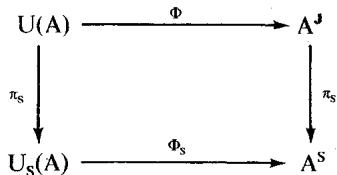
\includegraphics[keepaspectratio]{images/part001_3bc9714d.jpg}}

\(\mathrm{where}\ \Phi_{\mathbf{S}}((a_n)_{n\in \mathbf{S}}) = (\Phi_n((a_d)_{d\in \mathbf{J}_n}))_{n\in \mathbf{S}}.\)

\begin{enumerate}
\def\labelenumi{\alph{enumi})}
\setcounter{enumi}{1}
\item
  For every \(n \in \mathbf{J}\) , \(\operatorname{Ker}(\pi_{\mathrm{S}})\) is stable under \(\mathbf{V}_{n}\) , and \(\operatorname{Ker}(\pi_{\mathrm{S}})\) contains \(\mathbf{V}_{n}(\mathrm{U}(\mathrm{A}))\) if \(n \notin S\) . By passage to the quotient \(\mathbf{V}_{n}\) defines an endomorphism, still denoted \(\mathbf{V}_{n}\) , of the additive group of \(\mathrm{U}_{\mathrm{S}}(\mathrm{A})\) .
\item
  If \(n \in \mathbf{J}\) and if \(n\mathbf{S} \subset \mathbf{S}\) then \(\operatorname{Ker}(\pi_{\mathbf{S}})\) is stable under \(\mathbf{F}_{n}\) , which defines, by passing to the quotient, an endomorphism, still denoted \(\mathbf{F}_{n}\) , of the ring \(\mathrm{U}_{\mathrm{S}}(\mathrm{A})\) .
\end{enumerate}

\(d)\) Let \(n \in \mathbf{J}\) . The ring \(\mathrm{U}_{\mathrm{S}}(\mathrm{A})\) will also be denoted \(\mathrm{U}_{n}(\mathrm{A})\) if \(S = \mathbf{J}_{n}\) , and \(\mathrm{U}_{n\infty}(\mathrm{A})\) if \(\mathrm{S} = \bigcup_{n > 1} \mathbf{J}_{n}\) .

Let \(p\) a prime number. Show that \(\mathrm{U}_{p^{\infty}}(\mathbf{A})\) is identified with the Witt ring \(\mathrm{W}(\mathbf{A})\) and that, for every \(n \in \mathbf{N}\) , \(\mathrm{U}_{p^n}(\mathbf{A})\) is identified with the ring \(\mathrm{W}_{n+1}(\mathbf{A})\) (we identify the element ( \(u_1, u_p, u_{p^2}, ..., u_{p^{n-1}}, u_{p^n}\) ) of \(\mathrm{U}_{p^n}(\mathbf{A})\) to the Witt vector \([a_0, ..., a_n]\) with \(a_i = u_{p^i}\) for \(0 \leqslant i \leqslant n\) ). Group endomorphisms \(\mathbf{V}_p\) and \(\mathbf{F}_p\) of \(\mathrm{U}_{p^\infty}(\mathbf{A})\) correspond respectively, under this identification, to the shift and to the Frobenius endomorphism of \(\mathrm{W}(\mathbf{A})\) .

\begin{enumerate}
\def\labelenumi{\arabic{enumi})}
\setcounter{enumi}{39}
\tightlist
\item
  Let A be a ring. Let \(\mathbf{J} = \mathbf{P} \times \mathbf{Q}\) be a decomposition of the monoid J as a product of submonoids P and Q (which are therefore generated by the prime numbers they contain). One assumes that every \(q \in \mathbf{Q}\) is invertible in A, hence also in U(A) (p.~52, exerc. 35, e)). a) For every \(a \in \mathrm{U(A)}\) the series
\end{enumerate}

\[
\varepsilon_ {\mathbf {Q}} (\boldsymbol {a}) = \sum_ {q \in \mathbf {Q}} \frac {\mu (q)}{q} \mathbf {V} _ {q} \mathbf {F} _ {q} (a),
\]

where \(\mu\) denotes the Möbius function (Lie, II, p.~71), is convergent for the product topology of U(A) = A \(^{J}\) . One thus defines the additive endomorphism \(\varepsilon_{Q} = \sum_{q \in Q} \frac{\mu(q)}{q} V_{q} F_{q}\) of U(A). For every \(n \in J\) , the map \(\Phi_{n} \circ \varepsilon_{Q}\) from U(A) into A is equal to 0 if \(n \notin P\) and to \(\Phi_{n}\) if \(n \in P\) . b) For every \(q \in Q\) , \(q \neq 1\) , one has

\[
\varepsilon_ {\mathbf {Q}} \mathbf {V} _ {q} = 0 = \mathbf {F} _ {q} \varepsilon_ {\mathbf {Q}}.
\]

(Use exerc. 36, c), p.~52.)

\begin{enumerate}
\def\labelenumi{\alph{enumi})}
\setcounter{enumi}{2}
\tightlist
\item
  Show that \(\varepsilon_{\mathbf{Q}}\) is an idempotent whose image is the intersection of the kernels of the \(\mathbf{F}_{q}\) ( \(q \in \mathbf{Q}, q \neq 1\) ).
\end{enumerate}

For \(m \in \mathbf{J}\) and \(a \in \mathbf{A}\) , compute \(\varepsilon_{\mathrm{Q}} \mathrm{V}_{m} \tau(a)\) . Deduce that the kernel of \(\varepsilon_{\mathrm{Q}}\) is the set of elements of the form \(\sum_{n \in \mathrm{Q}} \mathrm{V}_{n} \tau(a_{n})\) , with \(a_{n} \in \mathbf{A}\) . The subset \(\varepsilon_{\mathrm{Q}} \mathrm{U}(\mathrm{A})\) of \(\mathrm{U}(\mathrm{A})\) is stable under addition and multiplication. Equipped with these two operations, it is a commutative ring, with identity \(\varepsilon_{\mathrm{Q}}(1_{\mathrm{U}(\mathrm{A})})\) and the map \(\varepsilon_{\mathrm{Q}}: \mathrm{U}(\mathrm{A}) \to \varepsilon_{\mathrm{Q}} \mathrm{U}(\mathrm{A})\) is a ring homomorphism.

\begin{enumerate}
\def\labelenumi{\alph{enumi})}
\setcounter{enumi}{3}
\tightlist
\item
  For every \(q \in Q\) , set \(e_{q} = \frac{1}{q} V_{q} \varepsilon_{Q} F_{q}\) . Show that we have \(e_{q}^{2} = e_{q}\) and \(e_{q} e_{q'} = 0\) if \(q \neq q'\) and that, for every \(a \in U(A)\) we have
\end{enumerate}

\[
(*) \quad \boldsymbol {a} = \sum_ {q \in Q} e _ {q} (\boldsymbol {a}),
\]

where the sum is convergent for the product topology of U(A). (For (*) reduce to the case where \(a = X \in \mathrm{U}(\mathbf{R}[\mathbf{X}])\) , R being the subring of Q formed by the rational numbers with denominator in Q. It then suffices to apply \(\Phi\) and to verify the analogue of (*) in \(\mathbf{R}[\mathbf{X}]^{\mathbf{J}}\) which follows from the formula \(\Phi_{pq} \circ e_{q'} = \Phi_{pq} \delta_{qq'}\) if \(p \in P\) , \(q \in Q\) , \(q' \in Q\) .

The subset \(e_q \mathrm{U(A)}\) of \(\mathrm{U(A)}\) is stable under addition and multiplication. Equipped with these two operations, it is a commutative ring, with identity \(e_q(1_{\mathrm{U(A)}})\) and the map \(e_q: \mathrm{U(A)} \to e_q \mathrm{U(A)}\) is a ring homomorphism.

\begin{enumerate}
\def\labelenumi{\alph{enumi})}
\setcounter{enumi}{4}
\tightlist
\item
  For every \(q \in \mathbf{Q}\) , one has \(\mathbf{F}_q e_q = \varepsilon_{\mathbf{Q}} \mathbf{F}_q\) and \(\left(\frac{1}{q} \mathbf{V}_q\right) \varepsilon_{\mathbf{Q}} = e_q \left(\frac{1}{q} \mathbf{V}_q\right)\) . Conclude from this that \(\boldsymbol{a} \mapsto \mathbf{F}_q(\boldsymbol{a})\)
\end{enumerate}

is a ring isomorphism \(e_q\mathrm{U(A)}\to \varepsilon_{\mathrm{Q}}\mathrm{U(A)}\) , with inverse \(\pmb {a}\mapsto \frac{1}{q}\mathbf{V}_q(\pmb {a})\)

\begin{enumerate}
\def\labelenumi{\alph{enumi})}
\setcounter{enumi}{5}
\item
  Show that the canonical projection \(\pi_{\mathbb{P}}: \mathrm{U}(\mathrm{A}) \to \mathrm{U}_{\mathbb{P}}(\mathrm{A})\) (exerc. 39) defines a ring isomorphism \(\varepsilon_{\mathbb{Q}} \mathrm{U}(\mathrm{A}) \to \mathrm{U}_{\mathbb{P}}(\mathrm{A})\) . Deduce a ring isomorphism from U(A) onto \(\mathrm{U}_{\mathbb{P}}(\mathrm{A})^{\mathbb{Q}}\) sending \(a\) to \((\pi_{\mathbb{P}} \varepsilon_{\mathbb{Q}} \mathrm{F}_{q}(a))_{q \in \mathbb{Q}}\) for every \(a \in \mathrm{U}(\mathrm{A})\) .
\item
  If A is a Q-algebra, one may take \(\mathbf{P} = \{1\}\) and \(\mathbf{Q} = \mathbf{J}\) . One deduces a ring isomorphism \(\mathrm{U}(\mathrm{A}) \to \mathrm{A}^{\mathbf{J}}\) , which is none other than \(\Phi\) .
\end{enumerate}

  \(h)\) Suppose that \(\mathbf{P} = \{p^n | n \in \mathbb{N}\}\) , where \(p\) is a prime number. Thus every prime number \(q \neq p\) is invertible in A. We obtain a ring isomorphism \(\mathrm{U(A)} \to \mathrm{W(A)}^{\mathrm{Q}}\) (cf.~exerc. 39, \(d\) )).

We shall denote \(\omega_{\mathrm{A}}\) the map from W(A) to U(A), which, via the isomorphism between U(A) and \(\mathrm{W(A)}^{\mathbf{Q}}\), corresponds to the inclusion of W(A) in \(\mathrm{W(A)}^{\mathbf{Q}}\) according to the first component.

\begin{enumerate}
\def\labelenumi{\arabic{enumi})}
\setcounter{enumi}{40}
\tightlist
\item
  Let A be a ring.
\end{enumerate}

\begin{enumerate}
\def\labelenumi{\alph{enumi})}
\tightlist
\item
  Let \(\mu: A \to U(A)\) a ring homomorphism such that \(\Phi_1 \circ \mu = \text{Id}_A\) . Put \(\sigma = \Phi \circ \mu\) and \(\sigma(a) = (\sigma_n(a))_{n \in J}\) for \(a \in A\) . The maps \(\sigma_n: A \to A (n \in J)\) satisfy the following conditions:
\end{enumerate}

\begin{enumerate}
\def\labelenumi{(\arabic{enumi})}
\item
  \(\sigma_{n}\) is a ring homomorphism for all \(n\in\mathbf{J}\) , and \(\sigma_{1}=\mathrm{Id}_{\mathbf{A}}\) .
\item
  For every prime number \(p\) and for all \(a \in \mathbf{A}\) , one has \(\sigma_p(a) \equiv a^p \mod p\mathbf{A}\) and
\end{enumerate}

\[
\sigma_ {p} \left(\sigma_ {n} (a)\right) \equiv \sigma_ {p n} (a) \bmod . p ^ {w _ {p} (p n)} \mathrm{A} \quad \text { for every } \quad n \in \mathbf {J}.
\]

\begin{enumerate}
\def\labelenumi{\alph{enumi})}
\setcounter{enumi}{1}
\item
  Suppose that the additive group of A is Z-torsion-free. Let \(\sigma = (\sigma_n)_{n \in \mathbf{J}}\) be a family of mappings \(\sigma_n: A \to A\) satisfying conditions (1) and (2) of \(a\) ). There exists a unique ring homomorphism \(\mu: A \to U(A)\) such that \(\Phi_1 \circ \mu = Id_A\) and \(\Phi \circ \mu = \sigma\) (Apply Exercises 32 and 33, \(d\) ), p.~51.)
\item
  Suppose that the additive group of A is Z-torsion-free. There exists a unique ring homomorphism
\end{enumerate}

\[
\mu^ {\mathrm{A}}: \mathrm{U} (\mathrm{A}) \rightarrow \mathrm{U} (\mathrm{U} (\mathrm{A}))
\]

such that \(\Phi^{\mathrm{U(A)}}\circ \mu^{\mathrm{A}}\) is the map

\[
\mathbf {F} ^ {\mathbf {A}}: \mathrm{U} (\mathbf {A}) \rightarrow \mathrm{U} (\mathbf {A}) ^ {\mathbf {J}}
\]

defined by \(\mathbf{F}^{\mathrm{A}}(\boldsymbol{a}) = (\mathbf{F}_n(\boldsymbol{a}))_{n\in \mathbf{J}}\) (Reduce to the case where \(\mathbf{A} = \mathbf{Z}[\mathbf{X}]\) . Apply \(b\) ) and Exercises 36 and 38, \(b\) ), pp. 52 and 53.)

\begin{enumerate}
\def\labelenumi{\alph{enumi})}
\setcounter{enumi}{3}
\tightlist
\item
  Let \(\mathbf{X} = (\mathbf{X}_n)_{n\in \mathbf{J}}\) be a family of indeterminates considered as an element of \(\mathrm{U}(\mathbf{Z}[\mathbf{X}])\). Let
\end{enumerate}

\[
\mu^ {\mathbf {Z} [ \mathbf {X} ]} (\mathbf {X}) = \left(\mu_ {n} (\mathbf {X})\right) _ {n \in \mathbf {J}} = \left(\left(\mu_ {n, m} (\mathbf {X})\right) _ {m \in \mathbf {J}}\right) _ {n \in \mathbf {J}}
\]

where \(\mu_{n,m}(\mathbf{X})\in\mathbf{Z}[\mathbf{X}]\) for \(n,m\in\mathbf{J}\). For every ring A define \(\mu^{\mathbf{A}}:\mathrm{U}(\mathbf{A})\to\mathrm{U}(\mathrm{U}(\mathbf{A}))\) by \(\mu^{\mathbf{A}}(\boldsymbol{a})=(\left(\mu_{n,m}(\boldsymbol{a})\right)_{m\in\mathbf{J}})_{n\in\mathbf{J}}\). Show that \(\mu^{\mathbf{A}}\) is a ring homomorphism such that the following diagram is commutative

\begin{enumerate}
\def\labelenumi{(\arabic{enumi})}
\tightlist
\item
\end{enumerate}

\pandocbounded{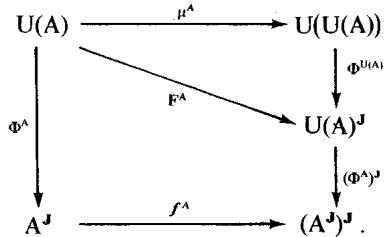
\includegraphics[keepaspectratio]{images/part001_e852df9c.jpg}}

Here by definition, \(f^{\mathrm{A}}(\boldsymbol{a}) = (f_n(\boldsymbol{a}))_{n \in \mathbf{J}}\) for \(\boldsymbol{a} \in \mathrm{A}^{\mathrm{J}}\) , and \(\Phi^{\mathrm{A}}\) (resp. \(\Phi^{\mathrm{U(A)}}\) ) is the homomorphism \(\Phi\) associated with the ring A (resp. U(A)).

\begin{enumerate}
\def\labelenumi{\alph{enumi})}
\setcounter{enumi}{4}
\tightlist
\item
  For every ring homomorphism \(\rho: \mathbf{B} \to \mathbf{A}\) the diagram
\end{enumerate}

\pandocbounded{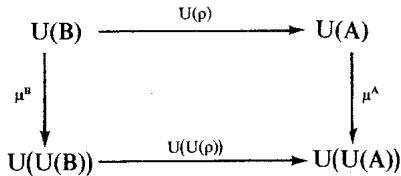
\includegraphics[keepaspectratio]{images/part001_6be88655.jpg}}

is commutative.

\begin{enumerate}
\def\labelenumi{\alph{enumi})}
\setcounter{enumi}{5}
\tightlist
\item
  Show that the following diagram is commutative.
\end{enumerate}

\pandocbounded{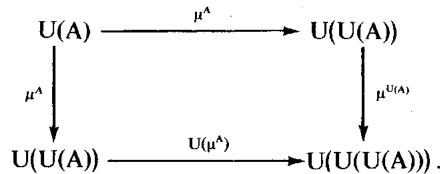
\includegraphics[keepaspectratio]{images/part001_4b4fe1b3.jpg}}

(Reduce to the case where A = \(\mathbf{Q}[\mathbf{X}]\). Then A is a Q-algebra, hence \(\Phi^{\mathbf{A}}: \mathrm{U}(\mathrm{A}) \to \mathrm{A}^{\mathbf{J}}\) is an isomorphism and U(A) is also a Q-algebra. If, using diagram (1) and by transport of structure, one replaces \(\mu^{\mathbf{A}}\) by \(f^{\mathbf{A}}\) when A is a Q-algebra, one is reduced to proving the commutativity of the diagram

\pandocbounded{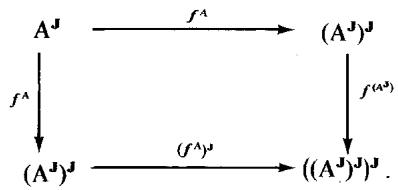
\includegraphics[keepaspectratio]{images/part001_85799ba9.jpg}}

We have

\[
f ^ {(\mathrm{A} ^ {\mathrm{J}})} \left(f ^ {\mathrm{A}} (\mathbf {X})\right) = f ^ {(\mathrm{A} ^ {\mathrm{J}})} \left(\left(f _ {n} (\mathbf {X})\right) _ {n \in \mathbf {J}}\right) = \left(\left(f _ {m} \left(f _ {n} (\mathbf {X})\right)\right) _ {n \in \mathbf {J}}\right) _ {m \in \mathbf {J}} = \left(\left(f _ {m n} (\mathbf {X})\right) _ {n \in \mathbf {J}}\right) _ {m \in \mathbf {J}},
\]

and

\[
(f ^ {\mathrm{A}}) ^ {\mathrm{J}} (f ^ {\mathrm{A}} (\mathbf {X})) = (f ^ {\mathrm{A}}) ^ {\mathrm{J}} ((f _ {n} (\mathbf {X})) _ {n \in \mathbf {J}}) = (f ^ {\mathrm{A}} (f _ {n} (\mathbf {X}))) _ {n \in \mathbf {J}} = ((f _ {m n} (\mathbf {X})) _ {m \in \mathbf {J}}) _ {n \in \mathbf {J}}.
\]

\begin{enumerate}
\def\labelenumi{\alph{enumi})}
\setcounter{enumi}{6}
\tightlist
\item
  For every \(a \in \mathbf{A}\) , one has
\end{enumerate}

\[
\mu_ {n} ^ {\mathrm{A}} (\tau (a)) = 0 \quad \text { for } \quad n \geqslant 2.
\]

\begin{enumerate}
\def\labelenumi{\alph{enumi})}
\setcounter{enumi}{7}
\tightlist
\item
  We have the following commutative diagram
\end{enumerate}

\pandocbounded{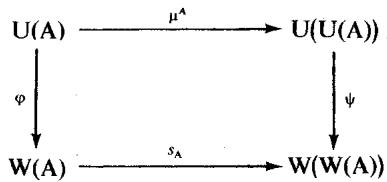
\includegraphics[keepaspectratio]{images/part001_0d6c50d0.jpg}}

where the map \(s_{\mathbf{A}}\) is the one defined in exerc. 15, p.~44, where the map \(\varphi\) from U(A) to W(A) is obtained by identifying W(A) with U \(_{p\infty}\) (A) (p.~53, exerc. 39), and the map \(\psi\) is the composite of U( \(\varphi\) ) and the map from U(W(A)) to W(W(A)) obtained by identifying W(W(A)) with U \(_{p\infty}\) (W(A)).

\begin{enumerate}
\def\labelenumi{\arabic{enumi})}
\setcounter{enumi}{41}
\tightlist
\item
  Let A be a ring and T an indeterminate. We denote by \(\Lambda(A)\) (or \(\Lambda_{T}(A)\) ) the set \(1 + TA[[T]]\) of formal power series with coefficients in A and constant term equal to 1; it is a subgroup of the multiplicative group of \(A[[T]]\). We define
\end{enumerate}

\[
\mathrm{L}: \Lambda (\mathrm{A}) \rightarrow \mathrm{A} ^ {\mathbf {J}}, \quad \mathrm{L} (f) = \left(\mathrm{L} _ {n} (f)\right) _ {n \in \mathbf {J}},
\]

by

\[
- \mathrm{T} \frac {d f}{d \mathrm{T}} / f = \sum_ {n \in \mathbf {J}} \mathrm{L} _ {n} (f) (- \mathrm{T}) ^ {n}.
\]

\begin{enumerate}
\def\labelenumi{\alph{enumi})}
\item
  Show that one has L(fg) = L(f) + L(g) for any f, g ∈ Λ(A).
\item
  If A is a Q-algebra, then L is bijective, its inverse ε being given by
\end{enumerate}

\[
\varepsilon (\boldsymbol {a}) = \exp (- \sum_ {n \in \mathbf {J}} \frac {a _ {n}}{n} (- \mathrm{T}) ^ {n})
\]

for \(a \in A^{J}\) .

\begin{enumerate}
\def\labelenumi{\arabic{enumi})}
\setcounter{enumi}{42}
\tightlist
\item
  Let E: U(A) → Λ(A) be the map defined by
\end{enumerate}

\[
\mathrm{E} (\boldsymbol {a}) = \prod_ {n \in \mathbf {J}} (1 - a _ {n} (- \mathrm{T}) ^ {n})
\]

for \(a \in \mathrm{U}(\mathrm{A})\) .

\begin{enumerate}
\def\labelenumi{\alph{enumi})}
\tightlist
\item
  Prove the commutativity of the diagram.
\end{enumerate}

\pandocbounded{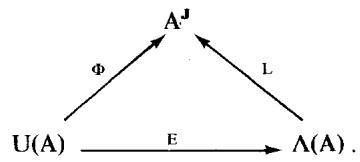
\includegraphics[keepaspectratio]{images/part001_4add4456.jpg}}

Deduce that if A is a Q-algebra, then

\[
\prod_ {n \in \mathbf {J}} (1 - a _ {n} \mathrm{T} ^ {n}) = \exp \left(- \sum_ {n \in \mathbf {J}} (\Phi_ {n} (\boldsymbol {a}) / n) \mathrm{T} ^ {n}\right)
\]

for all \(a \in \mathrm{U}(\mathrm{A})\) .

\begin{enumerate}
\def\labelenumi{\alph{enumi})}
\setcounter{enumi}{1}
\item
  Show that E is bijective. (If one sets \(\prod_{n\in J}(1 - a_n(-T)^n) = \sum_{n\geqslant 0}c_n(a)(-T)^n\) it suffices to apply exerc. 33, a), p.~51 to the family of polynomials \(c_{n}(\mathbf{X})\) of \(\mathbf{Z}[\mathbf{X}]\) .)
\item
  We equip \(\Lambda(A)\) with the unique ring structure such that E is a ring isomorphism. Show that the addition of \(\Lambda(A)\) is the multiplication of series, with identity element 1. The multiplication of the ring \(\Lambda(A)\) denoted \((f,g)\mapsto f*g\) , is defined by the formula
\end{enumerate}

\[
\mathrm{E} (\boldsymbol {a} \times \boldsymbol {b}) = \mathrm{E} (\boldsymbol {a}) * \mathrm{E} (\boldsymbol {b})
\]

for any \(a, b \in \mathrm{U}(\mathrm{A})\) ; its identity element is \(1 + T\) .

\begin{enumerate}
\def\labelenumi{\alph{enumi})}
\setcounter{enumi}{3}
\tightlist
\item
  Let \(\tau : \mathrm{A} \to \mathrm{U}(\mathrm{A})\) be the map defined in exerc. 37, c), p.~53. We have
\end{enumerate}

\[
\begin{array}{c} \mathrm{E} (\tau (a)) = 1 + a \mathrm{T} \\ (1 + a \mathrm{T}) * (1 + b \mathrm{T}) = 1 + a b \mathrm{T} \\ (1 + a \mathrm{T}) * f (\mathrm{T}) = f (a \mathrm{T}) \\ \mathrm{L} (1 + a \mathrm{T}) = (a ^ {n}) _ {n \in \mathbf {J}} \end{array}
\]

for any \(a, b\) in \(\mathbf{A}\) and \(f(\mathbf{T})\) in \(\Lambda(\mathbf{A})\) .

\begin{enumerate}
\def\labelenumi{\alph{enumi})}
\setcounter{enumi}{4}
\tightlist
\item
  Let \(f\) and \(g\) two elements of \(\Lambda(A)\) that are polynomials in \(T\) , and let \(m\) the degree of \(f\) . Put
\end{enumerate}

\[
\varphi (\mathrm{X}) = \mathrm{X} ^ {m} f (\mathrm{T} / \mathrm{X})
\]

and

\[
\gamma (\mathrm{X}) = g (- \mathrm{X}).
\]

These are polynomials in X with coefficients in A\([\mathrm{T}]\); \(\varphi\) is monic and \(f*g\) is the resultant \(\operatorname{res}(\varphi, \gamma)\) of the polynomials \(\varphi\) and \(\gamma\) (cf. A, IV, p. 75).

(One may start from the formula

\[
(1 + a \mathrm{T}) * g = g (a \mathrm{T}),
\]

deduce the result if \(A = \mathbf{Z}[X_{1}, \ldots, X_{m}]\) and \(f = \prod_{i=1}^{m} (1 + X_i \mathrm{T})\), and pass from there to the general case.)

\begin{enumerate}
\def\labelenumi{\arabic{enumi})}
\setcounter{enumi}{43}
\tightlist
\item
  Let A be a ring.
\end{enumerate}

\begin{enumerate}
\def\labelenumi{\alph{enumi})}
\item
  The set \(\hat{\mathbf{U}}(\mathbf{A})\) of elements of \(\mathrm{U}(\mathbf{A})\) with nilpotent coordinates, all but finitely many of which are zero, is an ideal of the ring \(\mathrm{U}(\mathbf{A})\) . For every \(n \in \mathbf{J}\) , it is stable under \(\mathrm{F}_n\) and \(\mathrm{V}_n\) .
\item
  Let \(\boldsymbol{a} \in \hat{\mathbf{U}}(\mathbf{A})\) . Then the element \(\mathrm{E}(\boldsymbol{a})\) of \(\Lambda(\mathbf{A})\) is a polynomial in T. Its value at \(-1\) is an invertible element of A, which is also, for every \(n \in \mathbf{J}\) , the value at \(-1\) of the polynomial \(\mathrm{E}(\mathrm{V}_n\boldsymbol{a})\) .
\item
  If \(\boldsymbol{a} \in \mathrm{U}(\mathbf{A})\) and \(\boldsymbol{b} \in \hat{\mathbf{U}}(\mathbf{A})\) , denote by \(\langle \boldsymbol{a}, \boldsymbol{b} \rangle\) the value at \(-1\) of the polynomial \(\mathrm{E}(\boldsymbol{a}\boldsymbol{b})\) . One thus defines a Z-bilinear map from \(\mathrm{U}(\mathbf{A}) \times \hat{\mathbf{U}}(\mathbf{A})\) into \(\mathbf{A}^*\) and one has
\end{enumerate}

\[
\begin{array}{l} \langle \mathbf {F} _ {n} \boldsymbol {a}, \boldsymbol {b} \rangle = \langle \boldsymbol {a}, \mathbf {V} _ {n} \boldsymbol {b} \rangle \\ \langle \mathbf {V} _ {n} \boldsymbol {a}, \boldsymbol {b} \rangle = \langle \boldsymbol {a}, \mathbf {F} _ {n} \boldsymbol {b} \rangle \quad \text { for every } n \in \mathbf {J}. \end{array}
\]

\begin{enumerate}
\def\labelenumi{\arabic{enumi})}
\setcounter{enumi}{44}
\tightlist
\item
  By pre-λ-ring one means a ring A equipped with maps \(\lambda_{n}: \mathbf{A} \to \mathbf{A} (n \in \mathbb{N})\) such that (i) \(\lambda_{0}(a) = 1\) ,
\end{enumerate}

\begin{enumerate}
\def\labelenumi{(\roman{enumi})}
\setcounter{enumi}{1}
\item
  \(\lambda_{1}(a) = a,\)
\item
  \(\lambda_{n}(a + b) = \sum_{p=0}^{n} \lambda_{p}(a) \lambda_{n-p}(b)\) ,
\end{enumerate}

for any \(a, b\) in A. Conditions (i) and (iii) are also expressed by saying that

\[
\lambda (a) = \sum_ {n \geqslant 0} \lambda_ {n} (a) \mathrm{T} ^ {n}
\]

defines a homomorphism from the additive group of A into the multiplicative group \(\Lambda(A)\) .

By \(\lambda\) -morphism of a pre- \(\lambda\) -ring A into another B, one means a homomorphism \(\rho: A \to B\) of rings such that \(\rho(\lambda_n(a)) = \lambda_n(\rho(a))\) for any \(a \in A\) , \(n \in \mathbf{N}\) , in other words such that the diagram

\pandocbounded{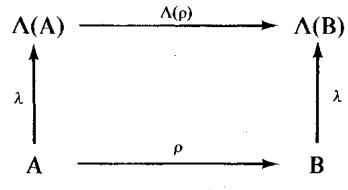
\includegraphics[keepaspectratio]{images/part001_12576e27.jpg}}

is commutative (the map \(\Lambda(\rho)\) transforms the series \(1 + \sum_{n\geqslant 1}a_n\mathrm{T}^n\) into the series \(1 + \sum_{n\geqslant 1}\rho(a_n)\mathrm{T}^n\) ). Let A be a ring. We propose to equip \(\Lambda(\mathbf{A})\) with a pre- \(\lambda\) -ring. Let us denote \(\mathbf{E}^{\mathbf{A}}:\mathrm{U}(\mathbf{A})\to \Lambda_{\mathbf{T}}(\mathbf{A})\) the ring isomorphism defined in exerc. 43. Let S be another indeterminate.

\begin{enumerate}
\def\labelenumi{\alph{enumi})}
\tightlist
\item
  Show that the two composed isomorphisms
\end{enumerate}

\[
\mathrm{U} (\mathrm{U} (\mathrm{A})) \xrightarrow {\mathrm{U} (\mathrm{E} ^ {\mathrm{A}})} \mathrm{U} (\Lambda_ {\mathrm{T}} (\mathrm{A})) \xrightarrow {\mathrm{E} ^ {\Lambda_ {\mathrm{T}} (\mathrm{A})}} \Lambda_ {\mathrm{S}} (\Lambda_ {\mathrm{T}} (\mathrm{A}))
\]

and

\[
\mathrm{U} (\mathrm{U} (\mathrm{A})) \xrightarrow {\mathrm{E} ^ {\mathrm{U} (\mathrm{A})}} \Lambda_ {\mathrm{S}} (\mathrm{U} (\mathrm{A})) \xrightarrow {\Lambda_ {\mathrm{S}} (\mathrm{E} ^ {\mathrm{A}})} \Lambda_ {\mathrm{S}} (\Lambda_ {\mathrm{T}} (\mathrm{A}))
\]

coincide; we will denote them \(\tilde{\mathbf{E}}^{\mathbf{A}}\) .

We define the map \(\lambda^{\mathrm{A}}\) by the commutativity of the diagram

\pandocbounded{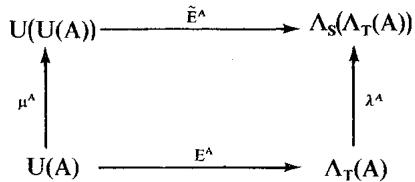
\includegraphics[keepaspectratio]{images/part001_a93606d8.jpg}}

where \(\mu^{\mathbf{A}}\) denotes the homomorphism defined in exerc. 41, \(d\) ), p.~55.

\begin{enumerate}
\def\labelenumi{\alph{enumi})}
\setcounter{enumi}{1}
\item
  The ring \(\Lambda(A)\), equipped with \(\lambda^{A}\), is a pre-\(\lambda\)-ring. For every ring homomorphism \(\rho: A \to B\), \(\Lambda(\rho): \Lambda(A) \to \Lambda(B)\) is a \(\lambda\)-morphism.
\item
  A pre-λ-ring A is called a λ-ring if λ: A → Λ(A) is a λ-morphism (for the pre-λ-ring structure on Λ(A) just defined).
\end{enumerate}

Let A be a ring. Show that \((\Lambda(A), \lambda^A)\) is a \(\lambda\)-ring. (Use Exerc. 41, \(f\) ), p.~56.)

\begin{enumerate}
\def\labelenumi{\arabic{enumi})}
\setcounter{enumi}{45}
\tightlist
\item
  \begin{enumerate}
  \def\labelenumii{\alph{enumii})}
  \tightlist
  \item
    Let A be a pre-λ-ring and \(a \in A\) . The λ-rank of a is called the least upper bound in \(\overline{R}\) of the set of integers \(n \in N\) such that \(\lambda_{n}(a) \neq 0\) . Let P be a multiplicative subset of A consisting of elements of λ-rank \(\leqslant 1\) . Let \(a = \sum_{i \in I} a_{i}\) be the sum of a finite family of elements of P. We have \(\lambda(a) = \prod_{i \in I} (1 + a_i T)\) , hence \(\lambda_n(a) = s_n((a_i)_{i \in I})\) , where \(s_n\) denotes the elementary symmetric polynomial
  \end{enumerate}
\end{enumerate}

of degree n (A, IV, p.~63).

\begin{enumerate}
\def\labelenumi{\alph{enumi})}
\setcounter{enumi}{1}
\item
  Let A be a ring and \(a, b\) elements of A. Then in \(\Lambda(A)\) the elements \(1 + aT\) and \((1 + aT)*(1 + bT) = 1 + abT\) are of \(\lambda\) -rank \(\leqslant 1\) .
\item
  Let A be a pre-λ-ring. Suppose there exists a multiplicative submonoid of A, consisting of elements of λ-rank ≤ 1, which generates the additive group of A. Show that A is then a λ-ring. More generally, A is a λ-ring if there exists an injective λ-morphism from A into a pre-λ-ring satisfying the preceding property ("Splitting principle"). (It is a matter of showing that the Z-bilinear map \((a, b) \mapsto \lambda(a) * \lambda(b) * \lambda(ab)^{-1}\) is zero and that the Z-linear maps \(a \mapsto \Lambda_{\mathrm{S}}(\lambda_{\mathrm{T}})[\lambda_{\mathrm{S}}(a)]\) and \(a \mapsto \lambda_{\mathrm{S}}^{\mathrm{A}}(\lambda_{\mathrm{T}}(a))\) from A to \(\Lambda_{\mathrm{S}}(\Lambda_{\mathrm{T}}(\mathrm{A}))\) coincide. It suffices to verify these properties for \(a, b \in P\) .)
\item
  Let \(A = \mathbf{Z}[(X_i)_{i\in I}, (X_{i'}')_{i'\in I'}]\) be the ring of polynomials in two finite families of indeterminates. We have
\end{enumerate}

\[
\prod_ {i \in I} (1 + X _ {i} T) = \sum_ {n \geqslant 0} s _ {n} ((X _ {i}) _ {i \in I}) T ^ {n}
\]

where

\[
s _ {n} \left(\left(X _ {i}\right) _ {i \in I}\right) = \sum_ {\mathrm{H} \in \binom {I} {n}} X _ {\mathrm{H}},
\]

\(\binom{I}{n}\) denoting the set of subsets with n elements of I, and where \(X_{H} = \prod_{h \in H} X_{h}\) . By assigning to the \(X_{i}\) (and \(X_{i'}\) ) the weight 1, \(s_{n}\) is homogeneous of weight n. Every symmetric polynomial in \((X_{i})_{i \in I}\) is expressed uniquely as a polynomial in the \(s_{n}\) ( \(n \geqslant 1\) ) (A, IV, p.~58). In particular, for every \(m \geqslant 0\) , one has

\[
s _ {m} \left(\left(\mathrm{X} _ {\mathrm{H}}\right) _ {\mathrm{H} \in \binom {\mathrm{I}} {n}}\right) = \mathrm{Q} _ {n, m} \left(s _ {1}, \dots , s _ {n m}\right)
\]

where \(Q_{n,m}\) is homogeneous of weight nm in the \(s_r = s_r((X_i)_{i \in I}) (r = 1, \ldots, nm)\) . This is the coefficient of \(T^m\) in \(\prod (1 + X_H T)\) , and it is well defined and independent of I, provided that \(\text{Card}(I) \geqslant nm\) .

The coefficient of \(\mathbf{T}^n\) in \(\prod (1 + X_iX_i'T)\) is

\[
s _ {n} \left(\left(X _ {i} X _ {i ^ {\prime}} ^ {\prime}\right) _ {(i, i ^ {\prime}) \in I \times I ^ {\prime}}\right) = P _ {n} \left(s _ {1}, \dots , s _ {n}, s _ {1} ^ {\prime}, \dots , s _ {n} ^ {\prime}\right)
\]

where \(s_r' = s_r((X_{i'}')_{i'\in I'})\) , and where \(P_n\) is homogeneous of weight \(n\) in each of the families of variables \((s_r)\) and \((s_r')\) . It is well defined and independent of I and I' provided that I and I' have cardinalities \(\geqslant n\) .

Show that in the \(\lambda\) -ring \(\Lambda(A)\) we have

\[
\left(\sum_ {r \geqslant 0} s _ {r} \mathrm{T} ^ {r}\right) * \left(\sum_ {r \geqslant 0} s _ {r} ^ {\prime} \mathrm{T} ^ {r}\right) = \sum_ {n \geqslant 0} \mathrm{P} _ {n} (s _ {1},..., s _ {n}, s _ {1} ^ {\prime},..., s _ {n} ^ {\prime}) \mathrm{T} ^ {n}
\]

and

\[
\lambda_ {n} ^ {\mathrm{A}} \left(\sum_ {r \geqslant 0} s _ {r} \mathrm{T} ^ {r}\right) = \sum_ {m \geqslant 0} \mathrm{Q} _ {n, m} \left(s _ {1}, \dots , s _ {n m}\right) \mathrm{T} ^ {m}.
\]

By a) and b), we have

\[
\left(\sum_ {r} s _ {r} \mathrm{T} ^ {r}\right) * \left(\sum_ {r} s _ {r} ^ {\prime} \mathrm{T} ^ {r}\right) = \left(\prod_ {i} \left(1 + \mathrm{X} _ {i} \mathrm{T}\right)\right) * \left(\prod_ {i ^ {\prime}} \left(1 + \mathrm{X} _ {i} ^ {\prime} \mathrm{T}\right)\right) = \prod_ {i, i ^ {\prime}} \left(1 + \mathrm{X} _ {i} \mathrm{X} _ {i ^ {\prime}} ^ {\prime} \mathrm{T}\right)
\]

and

\[
\begin{array}{l} \lambda (\sum_ {r} s _ {r} \mathrm{T} ^ {r}) = \lambda (\prod _{i} (1 + X _ {i} \mathrm{T})) = \prod _{i} (1 + (1 + X _ {i} \mathrm{T}) \mathrm{S}) = \sum _{n} s _ {n} ((1 + X _ {i} \mathrm{T}) _ {i \in \mathrm{I}}) \mathrm{S} ^ {n} \\ \text{and}\quad s _ {n} ((1 + X _ {i} \mathrm{T}) _ {i \in \mathrm{I}}) = \prod _{\mathrm{H} \in \binom {\mathrm{I}} {n}} (1 + X _{\mathrm{H}} \mathrm{T}) . \end{array}
\]

\begin{enumerate}
\def\labelenumi{\alph{enumi})}
\setcounter{enumi}{4}
\tightlist
\item
  Let A be a pre-λ-ring. For A to be a λ-ring, it is necessary and sufficient that the following conditions be satisfied, for all a, b in A, and n, m in N.
\end{enumerate}

\begin{enumerate}
\def\labelenumi{(\roman{enumi})}
\item
  \(\lambda(1) = 1 + T,\)
\item
  \(\lambda_{n}(ab) = \mathrm{P}_{n}(\lambda_{1}(a),\dots,\lambda_{n}(a),\lambda_{1}(b),\dots,\lambda_{n}(b)),\)
\item
  \(\lambda_{m}(\lambda_{n}(a)) = Q_{n,m}(\lambda_{1}(a),\dots,\lambda_{nm}(a)).\)
\end{enumerate}

\begin{enumerate}
\def\labelenumi{\alph{enumi})}
\setcounter{enumi}{5}
\tightlist
\item
  Let \(\rho: A \to B\) be a \(\lambda\)-morphism of pre-\(\lambda\)-rings. If A is a \(\lambda\)-ring and \(\rho\) is surjective, then B is a \(\lambda\)-ring. If B is a \(\lambda\)-ring and if \(\rho\) is injective, then A is a \(\lambda\)-ring.
\end{enumerate}

\begin{enumerate}
\def\labelenumi{\arabic{enumi})}
\setcounter{enumi}{46}
\tightlist
\item
  Let A be a ring. We define maps \(F_{n}\) , \(V_{n}\) (\(n \in \mathbf{J}\)) of \(\Lambda(\mathbf{A})\) into itself by the formulas
\end{enumerate}

\[
\mathrm{F} _ {n} (\mathrm{E} (a)) = \mathrm{E} \left(\mathrm{F} _ {n} (a)\right), \quad \mathrm{V} _ {n} (\mathrm{E} (a)) = \mathrm{E} \left(\mathrm{V} _ {n} (a)\right)
\]

for all \(\boldsymbol{a} \in \mathrm{U}(\mathbf{A})\) .

\begin{enumerate}
\def\labelenumi{\alph{enumi})}
\tightlist
\item
  We have \(\mathrm{L}(\mathrm{F}_n(f)) = f_n(\mathrm{L}(f))\) and \(\mathrm{L}(\mathrm{V}_n(f)) = v_n(\mathrm{L}(f))\) for all \(f \in \Lambda(\mathbf{A})\) .
\end{enumerate}

Let n, m be in J and set \(d = \operatorname{pgcd}(n, m)\) .

\begin{enumerate}
\def\labelenumi{\alph{enumi})}
\setcounter{enumi}{1}
\item
  Show that \(F_{n}\) is an endomorphism of the ring \(\Lambda(\mathbf{A})\) , and that we have \(F_{n} \circ F_{m} = F_{nm}\) . For every prime number p and for every \(f \in \Lambda(\mathbf{A})\) , one has \(F_{p}(f) \equiv f^{*p} \mod p * \Lambda(\mathbf{A})\) , where \(f^{*p}\) denotes the product in the ring \(\Lambda(\mathbf{A})\) of p terms equal to f, and where \(p * \Lambda(\mathbf{A})\) denotes the principal ideal of \(\Lambda(\mathbf{A})\) generated by the sum in \(\Lambda(\mathbf{A})\) of p terms equal to the neutral element 1 + T, in other words by \((1 + T)^{p}\) .
\item
  Prove that \(V_{n}\) is an endomorphism of the additive group of \(\Lambda(\mathbf{A})\) , and that we have \(V_{n} \circ V_{m} = V_{nm}\) . d) For every \(f \in \Lambda(\mathbf{A})\) , one has \(F_{n}(V_{m}(f)) = V_{m/d}(F_{n/d}(f))^{d}\) . In particular \(F_{n}(V_{n}(f)) = f^{n}\) , and \(F_{n} \circ V_{m} = V_{m} \circ F_{n}\) if \(d = 1\) . For any \(f,g\in\Lambda(\mathbf{A})\), we have
\item
  For any \(f, g\) in \(\Lambda(A)\) , one has
\end{enumerate}

\[
\begin{array}{l} \mathrm{V} _ {n} (f) * \mathrm{V} _ {m} (g) = \mathrm{V} _ {n m / d} (\mathrm{F} _ {m / d} (f) * \mathrm{F} _ {n / d} (g)) ^ {d}, \\ \mathrm{V} _ {n} (f * \mathrm{F} _ {m} (g)) ^ {n / d} = \mathrm{V} _ {n} (f) * \mathrm{V} _ {n / d} (\mathrm{F} _ {m / d} (g)), \\ \mathrm{V} _ {n} (\mathrm{F} _ {m} (g)) ^ {n / d} = \mathrm{V} _ {n} (1 + \mathrm{T}) * \mathrm{V} _ {n / d} (\mathrm{F} _ {m / d} (g)). \end{array}
\]

In particular, we have

and

\[
\begin{array}{r l} & {\mathrm{V} _ {n} (f) * \mathrm{V} _ {n} (g) = \mathrm{V} _ {n} (f * g) ^ {n}} \\ & {\mathrm{V} _ {n} (f) * \mathrm{V} _ {m} (g) = \mathrm{V} _ {n m} (\mathrm{F} _ {m} (f) * \mathrm{F} _ {n} (g)) \quad \text {if} \quad d = 1.} \end{array}
\]

\begin{enumerate}
\def\labelenumi{\alph{enumi})}
\setcounter{enumi}{5}
\tightlist
\item
  We have
\end{enumerate}

\[
\mathrm{V} _ {n} (f) (\mathrm{T}) = f (- (- \mathrm{T}) ^ {n})
\]

for all \(f \in \Lambda(\mathbf{A})\) . In particular

\[
\mathrm{V} _ {n} (1 + a \mathrm{T}) = 1 - a (- \mathrm{T}) ^ {n}
\]

for every \(a \in \mathbf{A}\) .

\begin{enumerate}
\def\labelenumi{\alph{enumi})}
\setcounter{enumi}{6}
\tightlist
\item
  For every \(a \in \mathbf{A}\) , one has
\end{enumerate}

\[
\mathrm{F} _ {n} (1 + a \mathrm{T}) = 1 + a ^ {n} \mathrm{T}.
\]

For every \(f \in \Lambda(\mathbf{A})\) , one has

\[
\mathrm{F} _ {n} (f) \left(- (- \mathrm{T}) ^ {n}\right) = \mathrm{N} (f (\mathrm{T}))
\]

where N denotes the norm in the extension \(A[[\mathrm{T}^{n}]] \subset A[[\mathrm{T}]]\). (It suffices to treat the case where \(f \in A[\mathrm{T}]\), then embed A into a ring B where f decomposes into a product of linear factors, to which the first formula can be applied.)

For every \(a \in \mathbf{A}\) , one has

\[
\mathrm{F} _ {n} (1 - a (- \mathrm{T}) ^ {m}) = (1 - a ^ {n / d} (- \mathrm{T}) ^ {m / d}) ^ {d}.
\]

(Observe that \(1 - a(-T)^{m} = V_{m}(1 + aT)\) and use c) and f).) h) For any \(a, b \in A\) , one has

\[
(1 - a (- \mathrm{T}) ^ {n}) * (1 - b (- \mathrm{T}) ^ {m}) = (1 - a ^ {m / d} b ^ {n / d} (- \mathrm{T}) ^ {m n / d}) ^ {d}.
\]

(Use the first formula for e).)

\begin{enumerate}
\def\labelenumi{\arabic{enumi})}
\setcounter{enumi}{47}
\tightlist
\item
  Let A be a pre-λ-ring. Denote by Ψ the composite A \(\xrightarrow{\lambda} \Lambda(A) \xrightarrow{L} A^{J}\) , so that \(\Psi(a) = (\psi_{n}(a))_{n \in J}\) , where
\end{enumerate}

\[
- \mathrm{T} \frac {d}{d \mathrm{T}} \lambda (a) / \lambda (a) = \sum_ {n \in \mathrm{J}} \psi_ {n} (a) (- \mathrm{T}) ^ {n}.
\]

More explicitly,

\[
- n \lambda_ {n} (a) = (- 1) ^ {n} \psi_ {n} (a) + (- 1) ^ {n - 1} \psi_ {n - 1} (a). \lambda_ {1} (a) + \dots + (- \psi_ {1} (a)). \lambda_ {n - 1} (a)
\]

for all \(n \in J\) . In particular,

\[
\begin{array}{l} \psi_ {1} (a) = \lambda_ {1} (a) = a \\ \psi_ {2} (a) = \lambda_ {1} (a) ^ {2} - 2 \lambda_ {2} (a) \\ \psi_ {3} (a) = \lambda_ {1} (a) ^ {3} - 3 \lambda_ {1} (a) \lambda_ {2} (a) + 3 \lambda_ {3} (a). \end{array}
\]

The maps \(\psi_{n}:A\to A\) are called Adams operations.

When (A, \(\lambda\) ) = ( \(\Lambda(B)\) , \(\lambda^{B}\) ), where B is a ring, we will also write \(\Psi^{B}\) for \(\Psi\) .

\begin{enumerate}
\def\labelenumi{\alph{enumi})}
\tightlist
\item
  Let B be a ring. Show that for every \(n \in J\) , one has
\end{enumerate}

\[
\psi_ {n} ^ {\mathbf {B}} = \mathrm{F} _ {n}: \Lambda (\mathbf {B}) \rightarrow \Lambda (\mathbf {B}).
\]

(Use the commutative diagram

\pandocbounded{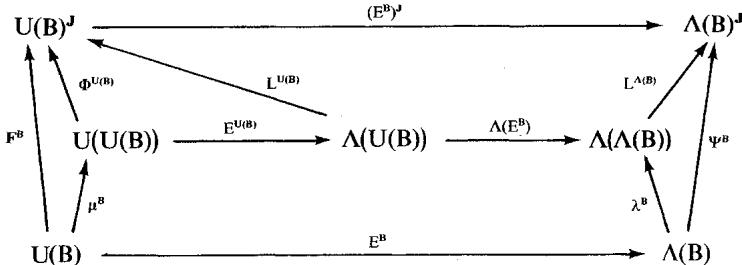
\includegraphics[keepaspectratio]{images/part001_4bd4d5b0.jpg}}

where all the horizontal maps are bijective.)

\begin{enumerate}
\def\labelenumi{\alph{enumi})}
\setcounter{enumi}{1}
\item
  Let A be a pre-λ-ring. For every \(n \in \mathbf{J}\) , \(\psi_n\) is an endomorphism of the additive group of A, and \(\psi_1 = \mathrm{Id}_A\) . If A is a λ-ring, \(\psi_n\) is an endomorphism of the ring A, and \(\psi_n \circ \psi_m = \psi_{nm}\) for any \(n\) , \(m\) in J. Moreover, for every prime number \(p\) we have \(\psi_p(a) \equiv a^p\) mod. \(p\mathbf{A}\) for all \(a \in \mathbf{A}\) (Using the injectivity of \(\lambda: \mathbf{A} \to \Lambda(\mathbf{A})\) and the analogous properties of \(\psi_n^{\mathbf{A}} = \mathbf{F}_n\) .)
\item
  Let A be a pre-λ-ring whose additive group is Z-torsion-free. For A to be a λ-ring, it is necessary and sufficient that the following conditions be satisfied for all integers \(n \geqslant 2\) and \(m \geqslant 2\) :
\end{enumerate}

\begin{enumerate}
\def\labelenumi{(\roman{enumi})}
\item
  \(\psi_n(1) = 1\) ;
\item
  \(\psi_{n}(ab) = \psi_{n}(a)\psi_{n}(b)\) for any \(a,b\) in A;
\item
  \(\psi_{n}\circ \psi_{m} = \psi_{nm}\)
\end{enumerate}

Since L : Λ(A) → A \(^{J}\) is an injective ring homomorphism, Ψ = L ∘ λ is a ring homomorphism if and only if λ is one. Similarly for the diagram.

\pandocbounded{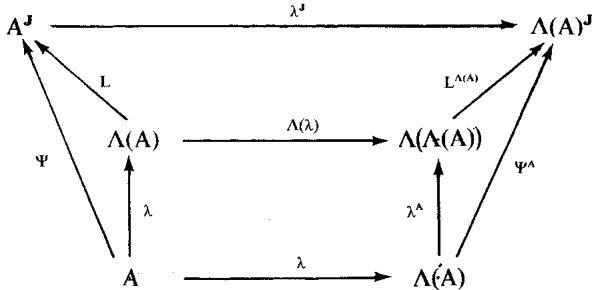
\includegraphics[keepaspectratio]{images/part001_ba507c2f.jpg}}

we deduce that

\(\Lambda (\lambda)\circ \lambda = \lambda^{\mathbf{A}}\circ \lambda\) (λ is a λ-morphism)

\(\Leftrightarrow \lambda^{\mathbf{J}}\circ \Psi = \Psi^{\mathbf{A}}\circ \lambda \Leftrightarrow \lambda \circ \psi_{n} = \psi_{n}^{\mathbf{A}}\circ \lambda\) for every \(n\)

\(\Leftrightarrow \mathrm{L} \circ \lambda \circ \psi_n = \mathrm{L} \circ \psi_n^{\mathrm{A}} \circ \lambda\) for every \(n\) .

Now \(\mathrm{L}\circ \lambda = \Psi\) and \(\mathbf{L}\circ \psi_n^{\mathbf{A}} = \mathbf{L}\circ \mathbf{F}_n = f_n\circ \mathbf{L}.\) Therefore,

\(\Lambda (\lambda)\circ \lambda = \lambda^{\mathrm{A}}\circ \lambda \Leftrightarrow \Psi \circ \psi_{n} = f_{n}\circ \Psi\) for every \(n\)

\(\Leftrightarrow \psi_{m} \circ \psi_{n} = \psi_{nm}\) for any \(m\) and \(n\) .

\begin{enumerate}
\def\labelenumi{\alph{enumi})}
\setcounter{enumi}{3}
\tightlist
\item
  Let A be a λ-ring. Let \(a \in \mathbf{A}\) be an element of λ-rank \(\leqslant 1\) (i.e.\(\lambda(a) = 1 + a\mathbf{T}\) ). Then \(\psi_n(a) = a^n\) for all \(n \in \mathbf{J}\) . If P is a multiplicative subset of A consisting of elements of λ-rank \(\leqslant 1\) and if \(a_1, \ldots, a_r\) belong to P, we have \(\psi_n(a_1 + \cdots + a_r) = a_1^n + \cdots + a_r^n\) .
\end{enumerate}

In the algebra of polynomials \(\mathbf{Z}[(\mathbf{X}_{i})_{i\in I}]\) , denote by \((s_{n})\) the elementary symmetric polynomials, \(\sum_{n\geq0}s_{n}\mathbf{T}^{n}=\prod_{i}(1+\mathbf{X}_{i}\mathbf{T})\) , and

\[
\mathrm{v} _ {n} (s _ {1}, \dots , s _ {n}) = \sum_ {i} \mathrm{X} _ {i} ^ {n}
\]

the n-th Newton polynomial. Show that, for any \(a \in A\) , one has

\[
\psi_ {n} (a) = v _ {n} \left(\lambda_ {1} (a), \dots , \lambda_ {n} (a)\right).
\]

(First verify this relation when \(a\) is of the form \(a_{1} + \cdots + a_{r}\) as above. Passing from there to the case where \(a = 1 + \sum_{h \geqslant 1} s_{h} \mathrm{T}^{h} \in \Lambda(\mathbf{Z}[(\mathrm{X}_{i})_{i \in I}])\) . Next, deduce the general case by embedding A into the \(\lambda\) -ring \(\Lambda(\mathbf{A})\) and using the homomorphism \(\mathbf{Z}[(s_{h})_{h=1,\ldots,n}] \to \mathbf{A}\) which sends \(s_{h}\) onto \(\lambda_{h}(a)\) .)

\begin{enumerate}
\def\labelenumi{\arabic{enumi})}
\setcounter{enumi}{48}
\tightlist
\item
  Let A be a ring, E a finitely generated projective A-module, and \(u \in \text{End}_{\mathbf{A}}(\mathbf{E})\) . If E is a free A-module, we denote by \(\det_{\mathbf{E}}(u)\) the determinant of \(u\) . In general, one can choose an A-module F such that \(\mathbf{E} \oplus \mathbf{F}\) is a finitely generated free A-module, and we set
\end{enumerate}

\[
\det _ {E} (u) = \det _ {E \oplus F} (u \oplus 1 _ {F}).
\]

\begin{enumerate}
\def\labelenumi{\alph{enumi})}
\tightlist
\item
  Show that \(\operatorname{det}_{\mathbf{E}}(u)\) is independent of the choice of F, that \(\operatorname{det}_{\mathbf{E}}(1_{\mathbf{E}}) = 1\) , and that \(\operatorname{det}_{\mathbf{E}}(u \circ v) = \operatorname{det}_{\mathbf{E}}(u) \cdot \operatorname{det}_{\mathbf{E}}(v)\) for any \(u, v\) in \(\operatorname{End}_{\mathbf{A}}(\mathbf{E})\) .
\end{enumerate}
% semantic-fragments: legacy-input-seam
\relax{}
\begin{enumerate}
\def\labelenumi{\alph{enumi})}
\setcounter{enumi}{1}
\tightlist
\item
  Suppose that L is a direct summand submodule of E stable under \(u\), and denote by \(u_{\mathrm{L}} \in \mathrm{End}_{\mathrm{A}}(\mathrm{L})\) and \(u_{\mathrm{E/L}} \in \mathrm{End}_{\mathrm{A}}(\mathrm{E/L})\) the endomorphisms defined by \(u\). Then one has \(\det_{\mathrm{E}}(u) = \det_{\mathrm{L}}(u_{\mathrm{L}}) \cdot \det_{\mathrm{E/L}}(u_{\mathrm{E/L}})\). Let T be an indeterminate, E{[}T{]} = A{[}T{]} \(\otimes_{\mathrm{A}}\) E, and identify \(u\) with \(1_{\mathrm{A[T]}} \otimes_{\mathrm{A}} u \in \mathrm{End}_{\mathrm{A[T]}}(\mathrm{E[T]})\). Put
\end{enumerate}

\[
\chi_ {\mathrm{E}} (u) = \det (\mathrm{T}. 1 - u)
\]

(characteristic polynomial of \(u\)) and

\[
\overline {{{{\chi}}}} _ {\mathrm{E}} (u) = \det (1 + u \mathrm{T}) = \sum_ {n \geqslant 0} \operatorname{Tr} \left(\Lambda ^ {n} (u)\right) \mathrm{T} ^ {n}
\]

where 1 denotes \(1_{\mathrm{E[T]}}\) (cf. A, III, p. 107).

\begin{enumerate}
\def\labelenumi{\alph{enumi})}
\setcounter{enumi}{2}
\item
  We have \(\overline{\chi}_{\mathrm{E}}(0) = 1\). Suppose that E is locally free of constant rank \(r\). We have \(\overline{\chi}_{\mathrm{E}}(1_{\mathrm{E}}) = (1 + \mathrm{T})^{r}\). If \(\sigma_r: \mathrm{A}[\mathrm{T}, \mathrm{T}^{-1}] \to \mathrm{A}[\mathrm{T}, \mathrm{T}^{-1}]\) denotes the mapping \((\sigma_r f)(\mathrm{T}) = \mathrm{T}^r. f((- \mathrm{T})^{-1})\), we have \(\sigma_r(\sigma_r(f)) = (-1)^r f\) and \(\sigma_r(\overline{\chi}_{\mathrm{E}}(u)) = \chi_{\mathrm{E}}(u)\).
\item
  Let \(\alpha: \mathrm{A} \to \mathrm{A}'\) be a ring homomorphism. We have \(\overline{\chi}_{\mathrm{A}'\otimes_{\mathrm{A}}\mathrm{E}}(\mathrm{Id}_{\mathrm{A}'} \otimes_{\mathrm{A}} u) = \alpha(\overline{\chi}_{\mathrm{E}}(u))\), where we denote \(\alpha\) also for the homomorphism \(\mathrm{A}[\mathrm{T}] \to \mathrm{A}'[\mathrm{T}]\) defined by \(\alpha\).
\item
  We have \(\overline{\chi}_{\mathrm{E}}(u) \in \Lambda(\mathrm{A})\) . For every \(n \in \mathbf{J}\) , one has
\end{enumerate}

\[
\begin{array}{l} \lambda_ {n} ^ {\mathrm{A}} (\overline {{\chi}} _ {\mathrm{E}} (u)) = \overline {{\chi}} _ {\Lambda^ {n} (\mathrm{E})} (\Lambda^ {n} (u)), \\ \psi_ {n} ^ {\mathrm{A}} (\overline {{\chi}} _ {\mathrm{E}} (u)) = \overline {{\chi}} _ {\mathrm{E}} (u ^ {n}). \end{array}
\]

(It suffices to verify the formulas locally on the spectrum of A, so we may assume E is equal to \(\mathbf{A}^r\). Let \((u_{ij})_{1\leqslant i,j\leqslant r}\) be the matrix of \(u\), let \((\mathrm{X}_{ij})_{1\leqslant i,j\leqslant r}\) be a family of indeterminates, set \(\mathbf{B} = \mathbf{Z}[(\mathrm{X}_{ij})]\), and let \(v\) be the endomorphism of \(\mathbf{B}^r\) with matrix \(\mathrm{X} = (\mathrm{X}_{ij})_{1\leqslant i,j\leqslant r}\). It suffices to verify the formulas for \(\mathbf{B}^r\) and \(v\in \operatorname {End}_{\mathbf{B}}(\mathbf{B}^r)\). One can embed B in an algebraically closed field C, and it suffices to verify the formulas for \(\mathbf{C}^r\) and \(w = \operatorname {Id}_{\mathbf{C}}\otimes_{\mathbf{B}}v\). Let \(a_1,\dots,a_r\) be the eigenvalues of \(w\), so that \(\overline{\chi}_{\mathbf{C}^r}(w) = \prod_i(1 + a_i\mathrm{T})\). We have \(\psi_n^{\mathrm{C}}(\overline{\chi}_{\mathbf{C}^r}(w)) = \prod_{i = 1}^{r}(1 + a_i^n\mathrm{T}) = \overline{\chi}_{\mathbf{C}^r}(w^n)\). Moreover \(\chi_{\Lambda^n (\mathbf{C}^r)}(\Lambda^n (w)) = \prod_{\mathrm{H}}(1 + a_{\mathrm{H}}\mathrm{T})\), where H ranges over the set of subsets with \(n\) elements of \(\{1,\dots,r\}\), and where \(a_{\mathrm{H}} = \prod_{h\in \mathrm{H}}a_h\). We can now apply Exerc. 46, \(d)\), p.~59, to show that \(\lambda_n^{\mathrm{C}}(\overline{\chi}_{\mathbf{C}^r}(w)) = \overline{\chi}_{\Lambda^{n}(\mathbf{C}^{r})}(\Lambda^{n}(w)).\)

\[
- \mathrm{T} \left[ \frac {d}{d \mathrm{T}} \overline {{{\chi}}} _ {\mathrm{E}} (u) \right] / \overline {{{\chi}}} _ {\mathrm{E}} (u) = \sum_ {n \in \mathbf {J}} \operatorname{Tr} (u ^ {n}) (- \mathrm{T}) ^ {n},
\]

in other words \(\mathrm{L}_n(\overline{\chi}_{\mathrm{E}}(u)) = \mathrm{Tr}(u^n)\) for \(n \in \mathbf{J}\) . (Reason as in \(e\) ).)

\begin{enumerate}
\def\labelenumi{\alph{enumi})}
\setcounter{enumi}{6}
\tightlist
\item
  Let E' be a finitely generated projective A-module, and \(u' \in \mathrm{End}_{\mathbf{A}}(\mathbf{E}')\). In the ring \(\Lambda(\mathbf{A})\),
\end{enumerate}

\[
\overline {{{{\chi}}}} _ {\mathrm{E} \otimes_ {\mathrm{A}} \mathrm{E} ^ {\prime}} (u \otimes_ {\mathrm{A}} u ^ {\prime}) = \overline {{{{\chi}}}} _ {\mathrm{E}} (u) * \overline {{{{\chi}}}} _ {\mathrm{E} ^ {\prime}} (u ^ {\prime}).
\]

(Reason as in e).)

\(h\) ) Let \(k\) be an algebraically closed field of characteristic \(p\ne0\), E a vector space over \(k\) of finite dimension \(n\), and \(u\) an endomorphism of E. We will denote by \(\tilde{\chi}_{\mathrm{E}}(u)\) the image of \(\overline{\chi}_{\mathrm{E}}(u)\) in \(\mathbf{W}(k)\) by the canonical homomorphisms (exerc. 43, p.~57 and exerc. 39, p.~53):

\[
\Lambda (k) \xrightarrow {\mathrm{E} ^ {- 1}} \mathrm{U} (k) \longrightarrow \mathrm{U} _ {p ^ {\infty}} (k) \longrightarrow \mathrm{W} (k).
\]

Prove that if \(\alpha_{1},\ldots,\alpha_{n}\) are the eigenvalues of the endomorphism \(u\) , one has

\[
\tilde {\chi} _ {E} (u) = \sum_ {i = 1} ^ {n} \tau (\alpha_ {i}) \quad \text { in } \quad W (k).
\]

\begin{enumerate}
\def\labelenumi{\arabic{enumi})}
\setcounter{enumi}{49}
\tightlist
\item
  Let A be a pre-λ-ring. By a λ-ideal of A one means an ideal a of A such that λ \(_{n}\) (a) ⊂ a for all n ∈ J.
\end{enumerate}

\begin{enumerate}
\def\labelenumi{\alph{enumi})}
\item
  Let a be a λ-ideal of A. Show that there exists a unique structure λ : A/a → Λ(A/a) of pre-λ-ring on A/a such that the canonical projection A → A/a is a λ-morphism.
\item
  The λ-ideals of A are precisely the kernels of λ-morphisms from A into other pre-λ-rings.
\item
  Let \((\mathfrak{a}_i)_{i\in I}\) be a family of \(\lambda\)-ideals of A. Then \(\bigcap \mathfrak{a}_i\) and \(\sum \mathfrak{a}_i\) are \(\lambda\)-ideals of A.
\item
  Let A be a λ-ring. If α and α′ are λ-ideals of A, then αα′ is a λ-ideal.
\item
  Let A be a \(\lambda\)-ring and let \(a \in \mathbf{A}\). The ideal \(\alpha\) of A generated by \(a, \lambda_2(a), \lambda_3(a), \ldots\) is a \(\lambda\)-ideal.
\end{enumerate}

\begin{enumerate}
\def\labelenumi{\arabic{enumi})}
\setcounter{enumi}{50}
\tightlist
\item
  Let A be a \(\lambda\)-ring and let \((\mathbf{X}_i)_{i\in I}\) be a family of indeterminates. Let us introduce the family of indeterminates \((\lambda_n\mathbf{X}_i)_{(n,i)\in \mathbf{J}\times \mathbf{I}}\) such that \(\lambda_1\mathbf{X}_i = \mathbf{X}_i\) for all \(i\in I\). Consider the polynomial algebra \(\mathrm{B} = \mathrm{A}\big[(\lambda_n\mathbf{X}_i)_{(n,i)\in \mathbf{J}\times \mathbf{I}}\big]\).
\end{enumerate}

The ring homomorphism \(\lambda: A \to \Lambda(A) \subset \Lambda(B)\) extends uniquely to a ring homomorphism \(\lambda: B \to \Lambda(B)\) such that

\[
\lambda (X _ {i}) = 1 + \sum_ {n \in \mathbf {J}} (\lambda_ {n} X _ {i}) T ^ {n}
\]

and, for \(q \geqslant 2\) ,

\[
\lambda (\lambda_ {q} \mathrm{X} _ {i}) = \lambda_ {q} ^ {\mathrm{B}} (\lambda (\mathrm{X} _ {i})).
\]

\begin{enumerate}
\def\labelenumi{\alph{enumi})}
\tightlist
\item
  Show that (B, λ) is a λ-ring. (This amounts to showing that the diagram of ring homomorphisms
\end{enumerate}

\pandocbounded{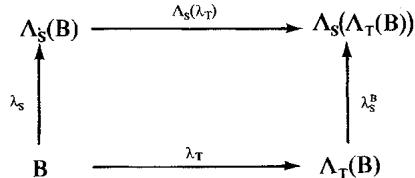
\includegraphics[keepaspectratio]{images/part001_09ec3539.jpg}}

is commutative. It suffices to check it on a generating set of the ring B.)

\begin{enumerate}
\def\labelenumi{\alph{enumi})}
\setcounter{enumi}{1}
\tightlist
\item
  Let C be a \(\lambda\)-ring, \(\rho:A \to C\) a \(\lambda\)-morphism, and \((c_i)_{i\in I}\) a family of elements of C. There exists one and only one \(\lambda\)-morphism \(\rho':B \to C\) extending \(\rho\) and such that \(\rho'(X_i) = c_i\) for all \(i\in I\).
\end{enumerate}

\begin{enumerate}
\def\labelenumi{\arabic{enumi})}
\setcounter{enumi}{51}
\tightlist
\item
  Let \((\mathbf{A}_i)_{i\in I}\) be a family of rings, \(\mathbf{A} = \prod_i\mathbf{A}_i\), and \(p_i:\mathbf{A}\to \mathbf{A}_i\) the canonical projection for every \(i\in \mathbf{I}\).\\
\end{enumerate}

\begin{enumerate}
\def\labelenumi{\alph{enumi})}
\item
  The map \(\alpha :\mathbf{A}[[T]]\to \prod_i\mathbf{A}_i[[T]]\) which maps \(\sum a_n\mathbf{T}^n\) onto \((\sum_{n}p_i(a_n)\mathbf{T}^n)_{i\in I}\) is a ring isomorphism. It defines, by restriction, a ring isomorphism \(\alpha :\Lambda (\mathbf{A})\to \prod_i\Lambda (\mathbf{A}_i)\). Moreover, we have, for all \(n\in \mathbf{J}\), \(\alpha \circ \lambda_n^{\mathbf{A}} = (\prod_i\lambda_n^{\mathbf{A}_i})\circ \alpha\) (Use the “universal polynomials” of Exerc. 46, d), p.~59.)
\item
  Suppose that, for every \(i \in I\), \(A_i\) is equipped with a structure \(\lambda_i: A_i \to \Lambda(A_i)\) of pre-\(\lambda\)-ring. By identifying \(\Lambda(A)\) with \(\prod_{i} \Lambda(A_i)\) by means of \(\alpha\), we define \(\lambda = \prod_{i} \lambda_i: A \to \Lambda(A)\). Then \((A, \lambda)\) is a pre-\(\lambda\)-ring, called the product of the family \(((A_i, \lambda_i))_{i \in I}\). For \((A, \lambda)\) to be a \(\lambda\)-ring, it is necessary and sufficient that \((A_i, \lambda_i)\) be one for all \(i \in I\).
\end{enumerate}

\begin{enumerate}
\def\labelenumi{\arabic{enumi})}
\setcounter{enumi}{52}
\tightlist
\item
  Let \(u = 1 + \mathrm{T} + \sum_{n=2}^{\infty} a_n \mathrm{T}^n\) be an element of \(\Lambda(\mathbf{Z})\). There exists one and only one group homomorphism \(\lambda^u: \mathbf{Z} \to \Lambda(\mathbf{Z})\) such that \(\lambda^u(1) = u\), and \((\mathbf{Z}, \lambda^u)\) is a pre-\(\lambda\)-ring. We have \(\lambda^u(n) = u^n\) for all \(n \in \mathbf{Z}\). For \((\mathbf{Z}, \lambda^u)\) to be a \(\lambda\)-ring, it is necessary and sufficient that \(u = 1 + \mathrm{T}\), in which case we have
\end{enumerate}

\[
\lambda_ {m} ^ {1 + \mathrm{T}} (n) = \binom {n} {m} = \frac {n (n - 1) \dots (n - m + 1)}{m !}
\]

for any \(n \in Z\) and \(m \in N\) .

\begin{enumerate}
\def\labelenumi{\arabic{enumi})}
\setcounter{enumi}{53}
\tightlist
\item
  Let C be a ring and A a C-algebra (not necessarily commutative). We denote \(\mathrm{Rep}_{\mathrm{C}}(\mathbf{A})\) the additive set of classes of A-modules that are finitely generated projective C-modules, and we denote \(\bar{\mathrm{R}}_{\mathrm{C}}(\mathring{\mathrm{A}})\) the Grothendieck group K( \(\mathrm{Rep}_{\mathrm{C}}(\mathbf{A})\) ) (cf.~A, VIII, § 10, n° 6). a) Let \(\alpha : \mathrm{A}' \to \mathrm{A}\) be a homomorphism of C-algebras. If E is an A-module of type \(\mathrm{Rep}_{\mathrm{C}}(\mathbf{A})\), then the module \(\alpha_{*}\mathrm{E}\), obtained by restriction of scalars from A to \(\mathrm{A}'\) (A, II, p.~30), is an A'-module of type \(\mathrm{Rep}_{\mathrm{C}}(\mathrm{A}')\), and {[}E{]} \(\mapsto [\alpha_{*}\mathrm{E}]\) defines a homomorphism \(\alpha_{*}: \mathrm{R}_{\mathrm{C}}(\mathrm{A}) \to \mathrm{R}_{\mathrm{C}}(\mathrm{A}')\).
\end{enumerate}

If \(\alpha_{1}:\mathbf{A}_{1}\to\mathbf{A}^{\prime}\) is a homomorphism of C-algebras, we have \((\alpha\circ\alpha_{1})_{*}=\alpha_{1*}\circ\alpha_{*}\) .

\begin{enumerate}
\def\labelenumi{\alph{enumi})}
\setcounter{enumi}{1}
\item
  One sets \(\mathbf{K}_0(\mathbf{C}) = \mathbf{R}_{\mathbf{C}}(\mathbf{C})\) . The structural homomorphism \(\varepsilon: \mathbf{C} \to \mathbf{A}\) defines a homomorphism \(\varepsilon_*: \mathbf{R}_{\mathbf{C}}(\mathbf{A}) \to \mathbf{K}_0(\mathbf{C})\) . If there exists a homomorphism \(\gamma: \mathbf{A} \to \mathbf{C}\) of C-algebras, then \(\gamma_*: \mathbf{K}_0(\mathbf{C}) \to \mathbf{R}_{\mathbf{C}}(\mathbf{A})\) is a right inverse of \(\varepsilon_*\) .
\item
  Let \(\gamma: \mathrm{C} \to \mathrm{C}'\) be a ring homomorphism. If E is an A-module of type \(\operatorname{Rep}_{\mathrm{C}}(\mathrm{A})\), then \(\gamma^{*}\mathrm{E} = \mathrm{C}' \otimes_{\mathrm{C}} \mathrm{E}\) is an \(\mathrm{A}_{\mathrm{C}'}\)-module of type \(\operatorname{Rep}_{\mathrm{C}'}(\mathrm{A}_{\mathrm{C}'})\), where \(\mathrm{A}_{\mathrm{C}'} = \mathrm{C}' \otimes_{\mathrm{C}} \mathrm{A}\), and {[}E{]} \(\mapsto [\gamma^{*}\mathrm{E}]\) defines a homomorphism \(\gamma^{*}: \mathrm{R}_{\mathrm{C}}(\mathrm{A}) \to \mathrm{R}_{\mathrm{C}'}(\mathrm{A}_{\mathrm{C}'})\). If \(\gamma_{1}': \mathrm{C}' \to \mathrm{C}_{1}\) is another ring homomorphism, we have \((\gamma_{1} \circ \gamma)^{*} = \gamma_{1}^{*} \circ \gamma^{*}\).
\item
  Let E \(\xrightarrow{f}\) F \(\xrightarrow{g}\) G be homomorphisms of A-modules, and set \(h = g \circ f\) . Construct an exact sequence of A-modules
\end{enumerate}

\[
(*) \quad 0 \rightarrow \operatorname{Ker} (f) \rightarrow \operatorname{Ker} (h) \rightarrow \operatorname{Ker} (g) \rightarrow \operatorname{Coker} (f) \rightarrow \operatorname{Coker} (h) \rightarrow \operatorname{Coker} (g) \rightarrow 0.
\]

Deduce from this that if \(f\) and \(g\) are injective, and if \(\operatorname{Coker}(f)\) and \(\operatorname{Coker}(g)\) are of type \(\operatorname{Rep}_{\mathbb{C}}(\mathbf{A})\), then \(\operatorname{Coker}(h)\) is of type \(\operatorname{Rep}_{\mathbb{C}}(\mathbf{A})\), and we have

\[
[ \operatorname{Coker} (h) ] = [ \operatorname{Coker} (f) ] + [ \operatorname{Coker} (g) ]
\]

in \(R_{C}(A)\) .

\begin{enumerate}
\def\labelenumi{\arabic{enumi})}
\setcounter{enumi}{54}
\tightlist
\item
  Let C be a ring. Let G be a monoid and let \(\mathbf{C}^{(\mathbf{G})}\) be its algebra over C. Instead of \(\mathrm{Rep}_{\mathbf{C}}(\mathbf{C}^{(\mathbf{G})})\) and \(\mathbf{R}_{\mathbf{C}}(\mathbf{C}^{(\mathbf{G})})\) , we write \(\mathrm{Rep}_{\mathbf{C}}(\mathbf{G})\) and \(\mathbf{R}_{\mathbf{C}}(\mathbf{G})\) . If \(\alpha : \mathbf{G}' \to \mathbf{G}\) is a homomorphism of monoids, we also denote by \(\alpha\) the homomorphism of C-algebras \(\mathbf{C}^{(\mathbf{G}')} \to \mathbf{C}^{(\mathbf{G})}\) that it defines, and \(\alpha_{*}: \mathbf{R}_{\mathbf{C}}(\mathbf{G}) \to \mathbf{R}_{\mathbf{C}}(\mathbf{G}')\) the corresponding homomorphism.
\end{enumerate}

By A, VIII, § 10, no. 5, there exists on R \(_{C}\) (G) a (commutative) ring structure such that

\[
[ \mathbf {E} ]. [ \mathbf {F} ] = [ \mathbf {E} \otimes_ {\mathrm{C}} \mathbf {F} ]
\]

if E and F are modules of finite type \(\mathrm{Rep}_{\mathbb{C}}(\mathbf{G})\) . The identity element for this multiplication is the class of the module \(C_1\) , equal to C with trivial action of G.

\begin{enumerate}
\def\labelenumi{\alph{enumi})}
\tightlist
\item
  The ring \(\mathbf{R}_{\mathrm{C}}(\mathbf{G})\) admits a unique structure of pre- \(\lambda\) -ring such that
\end{enumerate}

\[
\lambda [ \mathrm{E} ] = \sum_ {n \geqslant 0} \left[ \Lambda ^ {n} (\mathrm{E}) \right] \mathbf {T} ^ {n}
\]

for every module E of finite type \(\mathrm{Rep}_{\mathrm{C}}(\mathrm{G})\) . (First observe that \(\Lambda^{\mathrm{n}}(\mathrm{E})\) is again a module of finite type \(\mathrm{Rep}_{\mathrm{C}}(\mathrm{G})\) . Then, if F is a submodule such that F and E/F are of finite type \(\mathrm{Rep}_{\mathrm{C}}(\mathrm{G})\) , show that

\[
\left[ \Lambda ^ {n} (\mathrm{E}) \right] = \sum_ {p = 0} ^ {n} \left[ \Lambda ^ {p} (\mathrm{F}) \otimes_ {\mathrm{C}} \Lambda ^ {n - p} (\mathrm{E/F}) \right].
\]

in \(\mathbf{R}_{\mathbf{C}}(\mathbf{G})\).) For this, denote by \(\mathbf{L}_p\) the image of \(\Lambda^p(\mathbf{F}) \otimes_{\mathbf{C}} \Lambda^{n-p}(\mathbf{E})\), under the multiplication, in \(\Lambda^n(\mathbf{E})\). We have \(\Lambda^n(\mathbf{E}) = \mathbf{L}_0 \supset \mathbf{L}_1 \supset \ldots \supset \mathbf{L}_n = \Lambda^n(\mathbf{F}) \supset \mathbf{L}_{n+1} = 0\), and there exists a canonical isomorphism of \(\mathbf{C}^{(\mathbf{G})}\)-modules from \(\mathbf{L}_p / \mathbf{L}_{p+1}\) onto \(\Lambda^p(\mathbf{F}) \otimes \Lambda^{n-p}(\mathbf{E}/\mathbf{F})\).

\begin{enumerate}
\def\labelenumi{\alph{enumi})}
\setcounter{enumi}{1}
\item
  For every homomorphism \(\alpha: \mathbf{G}' \to \mathbf{G}\) of monoids, the map \(\alpha_*: \mathbf{R}_{\mathbf{C}}(\mathbf{G}) \to \mathbf{R}_{\mathbf{C}}(\mathbf{G}')\) is a \(\lambda\)-morphism. In particular \(\mathbf{K}_0(\mathbf{C})\) is a pre-\(\lambda\)-ring and \(\varepsilon_*: \mathbf{R}_{\mathbf{C}}(\mathbf{G}) \to \mathbf{K}_0(\mathbf{C})\) is a \(\lambda\)-morphism. The homomorphism \(\mathbf{G} \to \{1\}\) provides a right inverse for it.
\item
  Let \(\mathbf{G}\) a monoid and \(\mathbf{R}\) a set. A function \(f: \mathbf{G} \to \mathbf{R}\) will be called central if \(f(st) = f(ts)\) for any \(s, t \in \mathbf{G}\) . Let FC(G, R) denote the set of these functions. If R is a \(\lambda\) -ring, FC(G, R) is canonically endowed with a structure of \(\lambda\) -ring such that
\end{enumerate}

\[
\begin{array}{r l} (f + f ^ {\prime}) (s) & = f (s) + f ^ {\prime} (s) \\ (f \cdot f ^ {\prime}) (s) & = f (s) \cdot f ^ {\prime} (s) \\ (\lambda_ {n} f) (s) & = \lambda_ {n} (f (s)) \end{array}
\]

for any \(f, f'\) in \(\mathrm{FC}(\mathbf{G}, \mathbf{R})\) and \(s\) in \(\mathbf{G}\) . This applies in particular when \(\mathbf{R} = \Lambda(\mathbf{C})\) .

\begin{enumerate}
\def\labelenumi{\alph{enumi})}
\setcounter{enumi}{3}
\tightlist
\item
  Let E be a module of finite type \(\mathrm{Rep}_{\mathbb{C}}(\mathbf{G})\) . For every \(s \in \mathbf{G}\) , denote by \(s_{\mathbb{E}}\) the homothety of ratio \(s\) in E, and set
\end{enumerate}

\[
\overline {{{{\chi}}}} _ {\mathrm{E}} (s) = \det _ {\mathrm{E} [ \mathrm{T} ]} (1 + s _ {\mathrm{E}} \mathrm{T}) \in \Lambda (\mathrm{C})
\]

(cf. p. 62, exerc. 49). Show that

\[
\overline {{{{\chi}}}}: [ \mathrm{E} ] \mapsto \overline {{{{\chi}}}} _ {\mathrm{E}}
\]

defines a λ-morphism

\[
\overline {{{{\chi}}}}: \mathrm{R} _ {\mathrm{C}} (\mathrm{G}) \rightarrow \mathrm{FC} (\mathrm{G}, \Lambda (\mathrm{C})).
\]

\begin{enumerate}
\def\labelenumi{\alph{enumi})}
\setcounter{enumi}{4}
\tightlist
\item
  If C is a field, then \(\overline{\chi}\) is injective (A, VIII, § 10, no. 6, prop. 10). Deduce in this case that \(R_{C}(G)\) is a \(\lambda\)-ring.
\end{enumerate}

\begin{enumerate}
\def\labelenumi{\arabic{enumi})}
\setcounter{enumi}{55}
\tightlist
\item
  Let G be the free monoid generated by an element T, so that \(\mathrm{C}^{(\mathrm{G})}\) is identified with C{[}T{]}. Denote by \(C_{0}\) the module \(C{[}T{]}/T C{[}T{]}\). Then \([C_{0}]\) is an idempotent element of \(\mathrm{R}_{\mathrm{C}}(\mathrm{C}[\mathrm{T}])\). The kernel of the canonical \(\lambda\)-morphism \(\mathrm{R}_{\mathrm{C}}(\mathrm{C}[\mathrm{T}]) \rightarrow \mathrm{K}_{0}(\mathrm{C})\) is the ideal generated by \(1 - [\mathrm{C}_{0}]\). Put
\end{enumerate}

\[
\tilde {\mathrm{R}} _ {\mathrm{C}} (\mathrm{C} [ \mathrm{T} ]) = \mathrm{R} _ {\mathrm{C}} (\mathrm{C} [ \mathrm{T} ]) / [ \mathrm{C} _ {0} ]. \mathrm{R} _ {\mathrm{C}} (\mathrm{C} [ \mathrm{T} ]).
\]

\begin{enumerate}
\def\labelenumi{\alph{enumi})}
\item
  Show that \([C_{0}].R_{C}(C[T])\) is a \(\lambda\)-ideal, hence that \(\tilde{R}_{C}(C[T])\) admits a quotient pre-\(\lambda\)-ring.
\item
  For every module E of finite type \(\operatorname{Rep}_{\mathbf{C}}(\mathbf{C}[\mathbf{T}])\) , denote by \(\mathbf{T}_{\mathbf{E}}\) the homothety of ratio T in E. We have
\end{enumerate}

and

\[
\begin{array}{l} \overline {{\chi}} _ {\mathrm{E}} (\mathrm{T}) = \det _ {\mathrm{E} [ \mathrm{T} ]} (1 + \mathrm{T} _ {\mathrm{E}} \mathrm{T}) \in \Lambda (\mathrm{C}) \\ \chi_ {\mathrm{E}} (\mathrm{T}) = \det _ {\mathrm{E} [ \mathrm{T} ]} (\mathrm{T} - \mathrm{T} _ {\mathrm{E}}) \end{array}
\]

is the characteristic polynomial of \(T_{E}\) (cf.~exerc. 49, p.~62). Show that \([E] \mapsto \overline{\chi}_{E}(T)\) defines a \(\lambda\) -morphism \(R_{C}(C[T]) \to \Lambda(C)\) whose kernel contains \([C_{0}]\) . By passing to the quotient, we obtain a \(\lambda\) -morphism

\[
\overline {{\chi}}: \tilde {\mathrm{R}} _ {\mathrm{C}} (\mathrm{C} [ \mathrm{T} ]) \to \Lambda (\mathrm{C}).
\]

\begin{enumerate}
\def\labelenumi{\alph{enumi})}
\setcounter{enumi}{2}
\item
  Denote by \(\Lambda_{\mathrm{rat}}(\mathbf{C})\) the subgroup of \(\Lambda(\mathbf{C})\) generated by the elements of \(\Lambda(\mathbf{C})\) which are polynomials in T. Show that the image of \(\overline{\chi}\) is \(\Lambda_{\mathrm{rat}}(\mathbf{C})\). Conclude from this that \(\Lambda_{\mathrm{rat}}(\mathbf{C})\) is a sub-\(\lambda\)-ring of \(\Lambda(\mathbf{C})\).
\item
  For every \(r \in \mathbf{Z}\), define \(\sigma_r: \mathrm{C}[\mathrm{T}, \mathrm{T}^{-1}] \to \mathrm{C}[\mathrm{T}, \mathrm{T}^{-1}]\) by \((\sigma_r f)(\mathrm{T}) = \mathrm{T}^{r} f((-\mathrm{T})^{-1})\). We have \((\sigma_r(\sigma_s f))(\mathrm{T}) = (-1)^s \mathrm{T}^{r-s} f(\mathrm{T})\), in particular \(\sigma_r(\sigma_r f) = (-1)^r f\), and \((\sigma_r f).(\sigma_s g) = \sigma_{r+s}(f.g)\), for all \(r, s\) in \(\mathbf{Z}\) and \(f, g\) in \(\mathrm{C}[\mathrm{T}, \mathrm{T}^{-1}]\). If \(f\) is a polynomial in \(T\) of degree \(\leqslant r\) (\(r \geqslant 0\)), then \(\sigma_r f\) is one as well. If moreover \(f \in \Lambda(\mathrm{C})\) (i.e. \(f(0) = 1\)), then \(\sigma_r f\) is monic of degree \(r\). If E is a C{[}T{]}-module which is a free C-module of rank \(r\), one has \(\sigma_r(\overline{\chi}_{\mathrm{E}}(\mathrm{T})) = \chi_{\mathrm{E}}(\mathrm{T})\). e) If \(f \in \Lambda(\mathrm{C})\) is a polynomial in \(T\) of degree \(\leqslant r\), set \(E_{r,f} = C[T]/\sigma_r f.C[T]\); it is a free C-module of rank \(r\). If \(f = 1\) we have \(E_{r,1} = C[T]/T^{r}C[T]\). If \(g \in \Lambda(\mathrm{C})\) is a polynomial in \(T\) of degree \(\leqslant s\), we have an exact sequence of C{[}T{]}-modules
\end{enumerate}

\[
(*) \quad 0 \rightarrow \mathrm{E} _ {s, g} \rightarrow \mathrm{E} _ {r + s, f g} \rightarrow \mathrm{E} _ {r, f} \rightarrow 0
\]

(using \(d\) ). Show that the class \(\tau(f)\) of \(\mathrm{E}_{r,f}\) in \(\tilde{\mathrm{R}}_{\mathrm{C}}(\mathrm{C}[\mathrm{T}])\) is independent of \(r\) ( \(\geqslant \deg(f)\) ). (Indeed \(\sigma_{r+s}f = (\sigma_s1).(\sigma_rf) = \mathrm{T}^s.(\sigma_rf)\) and the class of the module \(\mathrm{C}[\mathrm{T}] / \mathrm{T}^s\mathrm{C}[\mathrm{T}]\) in \(\tilde{\mathrm{R}}_{\mathrm{C}}(\mathrm{C}[\mathrm{T}])\) is zero.) Show that if \(g\) is a polynomial in \(\Lambda(\mathrm{C})\) , one has \(\tau(fg) = \tau(f) + \tau(g)\) . (Use again the exact sequence (*).) Deduce from this that \(\tau\) extends to a group homomorphism

\[
\tau : \Lambda_ {\mathrm{rat}} (\mathrm{C}) \rightarrow \tilde {\mathrm{R}} _ {\mathrm{C}} (\mathrm{C} [ \mathrm{T} ]).
\]

\begin{enumerate}
\def\labelenumi{\alph{enumi})}
\setcounter{enumi}{5}
\tightlist
\item
  Show that \(\overline{\chi} \circ \tau\) is the identity map of \(\Lambda_{\mathrm{rat}}(\mathbf{C})\) (Using the fact that if \(f \in \Lambda(\mathbf{C})\) is a polynomial of degree \(\leqslant r\), then the characteristic polynomial of \(\mathrm{T}_{\mathrm{E}_r,f}\) is \(\sigma_r f\).)
\item
  Show that every element of \(\tilde{\mathrm{R}}_{\mathrm{C}}(\mathrm{C}[\mathrm{T}])\) is the class of a C{[}T{]}-module E which is a free C-module.
\end{enumerate}

\(h\) ) Let E be a C{[}T{]}-module, and denote by \(u\in \mathrm{End}_{\mathrm{C}}(\mathrm{E})\) the homothety of ratio T in E; let \(\overline{u} = \mathrm{Id}_{\mathrm{C[T]}}\otimes_{\mathrm{C}}u\in \mathrm{End}_{\mathrm{C[T]}}(\mathrm{E}[\mathrm{T}])\). We have an exact sequence of C{[}T{]}-modules

\[
0 \longrightarrow \mathrm{E} [ \mathrm{T} ] \xrightarrow {\mathrm{T} - \bar {u}} \mathrm{E} [ \mathrm{T} ] \longrightarrow \mathrm{E} \longrightarrow 0
\]

(A, III, p.~106). Suppose that E is a free C-module with basis \((e_1, \ldots, e_r)\). Then E{[}T{]} is a free C{[}T{]}-module with basis \((1 \otimes e_i)\). If the matrix of \(u\) for the basis \((e_i)\) is \((a_{ij})\), the matrix of T - \(\overline{u}\) for the basis \((1 \otimes e_i)\) is \((\mathrm{T}\delta_{ij} - a_{ij})\).

\begin{enumerate}
\def\labelenumi{\roman{enumi})}
\tightlist
\item
  Let \(f = (f_{ij})_{1 \leqslant i,j \leqslant r}\) be a matrix with coefficients in C{[}T{]}. We say that \(f\) is special if, for all \(i, j\) in \(\{1, \dots, r\}\), \(i \neq j\), \(f_{ii}\) is a monic polynomial and \(\deg(f_{ii}) > \deg(f_{ij})\). Then show that \(\det(f)\) is a monic polynomial (of degree \(\deg(f_{11}) + \cdots + \deg(f_{rr})\)) and that \(f\) defines an injective endomorphism of C{[}T{]} \(^r\). Deduce from h) that every C{[}T{]}-module which is a free C-module of rank \(r\) is isomorphic to the cokernel of such an endomorphism of C{[}T{]} \(^r\).
\end{enumerate}

\begin{enumerate}
\def\labelenumi{\alph{enumi})}
\setcounter{enumi}{9}
\tightlist
\item
  Let f be a special matrix as in i). Set \(f = \begin{pmatrix} f_{11} & f_{+} \\ f_{-} & f' \end{pmatrix}\) where \(f_{+}\) , \(f_{-}\) , \(f'\) are matrices of types \((1, r - 1)\) , \((r - 1, 1)\) and \((r - 1, r - 1)\) respectively. Set
\end{enumerate}

\[
g = \left( \begin{array}{c c} 1 & 0 \\ - f _ {-} & f _ {1 1} \mathrm{I} \end{array} \right) \quad \text {and} \quad h = g f = \left( \begin{array}{c c} f _ {1 1} & f _ {+} \\ 0 & \overline {{f}} \end{array} \right) \quad \text {where} \quad \overline {{f}} = f _ {1 1} f ^ {\prime} - f _ {-} f _ {+}.
\]

Show that h is a special matrix. Moreover, by identifying square matrices with the corresponding endomorphisms, one obtains exact sequences of C{[}T{]}-modules

\[
0 \rightarrow \operatorname{Coker} (f) \rightarrow \operatorname{Coker} (h) \rightarrow \operatorname{Coker} (g) \rightarrow 0,
\]

(where Coker(g) is isomorphic to \(\mathbf{C}[\mathbf{T}]^{r - 1} / f_{11}\mathbf{C}[\mathbf{T}]^{r - 1}\) ) and

\[
0 \rightarrow \mathrm{C} [ \mathrm{T} ] / f _ {1 1} \mathrm{C} [ \mathrm{T} ] \rightarrow \operatorname{Coker} (h) \rightarrow \operatorname{Coker} (\bar {f}) \rightarrow 0.
\]

From this, deduce by induction on \(r\) that \(\operatorname{Coker}(f)\) is a projective C-module whose class in \(\mathbf{R}_{\mathrm{C}}(\mathbf{C}[\mathrm{T}])\) is a \(\mathbf{Z}\)-linear combination of elements of the form \([\mathbf{C}[\mathrm{T}] / p\mathbf{C}[\mathrm{T}]]\), where \(p\) is a monic polynomial.

  \(k\) ) Use parts \(f\), \(g\), \(i)\), and \(j)\) above to show that \(\tau : \Lambda_{\mathrm{rat}}(\mathbf{C}) \to \tilde{\mathbf{R}}_{\mathrm{C}}(\mathbf{C}[\mathrm{T}])\) is surjective, hence that \(\overline{\chi} : \tilde{\mathbf{R}}_{\mathrm{C}}(\mathbf{C}[\mathrm{T}]) \to \Lambda_{\mathrm{rat}}(\mathbf{C})\) is an isomorphism.

\begin{enumerate}
\def\labelenumi{\alph{enumi})}
\setcounter{enumi}{11}
\tightlist
\item
  Show that \(\Lambda_{\mathrm{rat}}(\mathbf{C})\) is stable under \(\mathbf{V}_n\) and \(\mathbf{F}_n\) for each \(n \in \mathbf{J}\). There therefore correspond to them endomorphisms \(\mathbf{V}_n\) and \(\mathbf{F}_n\) of \(\tilde{\mathbf{R}}_{\mathbf{C}}(\mathbf{C}[\mathbf{T}])\), by the preceding isomorphism. Let \(\varphi_n\) be the homomorphism of C-algebras from C{[}T{]} to itself which maps T to \(\mathbf{T}^n\). Show that \(\mathbf{V}_n\) (resp. \(\mathbf{F}_n\)) is deduced from the endomorphism \(\varphi_n^*\) (resp. \((\varphi_n)_*\)) of \(\mathbf{R}_{\mathbf{C}}(\mathbf{C}[\mathbf{T}])\) by passing to quotients.
\end{enumerate}

In the following exercises, p is a fixed prime number, and the rings of Witt vectors are relative to this prime number.

\begin{enumerate}
\def\labelenumi{\arabic{enumi})}
\setcounter{enumi}{56}
\tightlist
\item
  Let \(m\), \(n\) be two integers \(\geqslant 1\). For every ring A of characteristic \(p\), denote by \(_{m}\mathrm{W}_{n}(\mathrm{A})\) the kernel of the endomorphism \(\mathrm{F}^{m}\) of \(\mathrm{W}_{n}(\mathrm{A})\).
\end{enumerate}

\begin{enumerate}
\def\labelenumi{\alph{enumi})}
\tightlist
\item
  For \(m \geqslant 2\) and \(n \geqslant 1\) the following diagram is commutative
\end{enumerate}

\pandocbounded{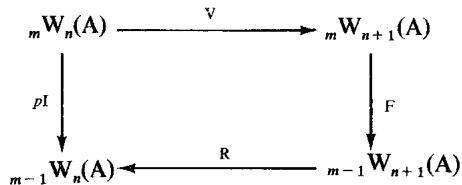
\includegraphics[keepaspectratio]{images/part001_6a9997c3.jpg}}

where the maps V, F are induced by the shift and Frobenius homomorphisms, respectively, I is the natural injection, and R is the natural projection.

\begin{enumerate}
\def\labelenumi{\alph{enumi})}
\setcounter{enumi}{1}
\tightlist
\item
  For \(n \geqslant 1\) and \(a = [a_0, \ldots, a_{n-1}]\) in \(W_n(A)\) , denote by \(\tilde{a}\) the element \((a_0, \ldots, a_{n-1}, 0, \ldots)\) of \(W(A)\) .
\end{enumerate}

Let \(a \in_{m} W_{n}(A)\) , \(b \in_{n} W_{m}(A)\) We then set

\[
\langle \boldsymbol {a}, \boldsymbol {b} \rangle = \mathrm{E} (\omega_ {\mathrm{A}} (\tilde {\boldsymbol {a}}) \omega_ {\mathrm{A}} (\tilde {\boldsymbol {b}}), 1)
\]

(cf. p. 57, exerc. 43 for the notation E, and p. 54, exerc. 40 for the notation \(\omega_{\mathbf{A}}\) ). Prove that the map \((\boldsymbol{a}, \boldsymbol{b}) \mapsto \langle \boldsymbol{a}, \boldsymbol{b} \rangle\) from \({}_{m}W_n(A) \times {}_{n}W_m(A)\) into \(A^*\) is \(\mathbf{Z}\)-bilinear. c) With the notation of a), we have

\[
\langle \boldsymbol {a}, \mathrm{V} \boldsymbol {b} \rangle = \langle \mathrm{F} \boldsymbol {a}, \boldsymbol {b} \rangle . \text { for } \quad \boldsymbol {a} \in_ {m} \mathrm{W} _ {n} (\mathrm{A}) \quad \text { and } \quad \boldsymbol {b} \in_ {n} \mathrm{W} _ {m - 1} (\mathrm{A})
\]

and

\[
\langle \mathbf {R} \boldsymbol {a}, \boldsymbol {b} \rangle = \langle \boldsymbol {a}, \mathbf {I} \boldsymbol {b} \rangle \quad \text { for } \quad \boldsymbol {a} \in_ {m} \mathrm{W} _ {n} (\mathrm{A}) \quad \text { and } \quad \boldsymbol {b} \in_ {n - 1} \mathrm{W} _ {m} (\mathrm{A}).
\]

\begin{enumerate}
\def\labelenumi{\arabic{enumi})}
\setcounter{enumi}{57}
\tightlist
\item
  \begin{enumerate}
  \def\labelenumii{\alph{enumii})}
  \tightlist
  \item
    Let \(\delta(T)\) be the formal series \(\exp\left(-\sum_{n=0}^{\infty}\mathrm{T}^{p^n}/p^n\right)\) of \(\mathbf{Q}[[T]]\). We have
  \end{enumerate}
\end{enumerate}

\[
\mathfrak{E}(\mathrm{T}) = \prod_{\substack{(n,p) = 1\\ n\text{ an integer}\geqslant 1}}(1 - \mathrm{T}^{n})^{\mu (n) / n}
\]

where μ is the Möbius function. The coefficients of δ(T) belong to \(\mathbf{Z}_{(p)}\). b) Let \(\mathbf{X} = (\mathbf{X}_{n})_{n \in \mathbb{N}}\) be a family of indeterminates. In the algebra \(\mathbf{Q}[(\mathbf{X}_{n})_{n \in \mathbb{N}}]\), we have the equality

\[
\prod_ {n = 0} ^ {\infty} \mathcal {E} (\mathrm{X} _ {n} \mathrm{T} ^ {p ^ {n}}) = \exp \left(- \sum_ {n = 0} ^ {\infty} \Phi_ {n} (\mathrm{X}) \mathrm{T} ^ {p ^ {n}} / p ^ {n}\right).
\]

\begin{enumerate}
\def\labelenumi{\alph{enumi})}
\setcounter{enumi}{2}
\item
  Let A be a \(\mathbf{Z}_{(p)}\) -algebra. It is assumed that multiplication by \(p, 1_{\mathbf{A}}\) is injective in A. Let \(\boldsymbol{a} = (a_n)_{n \in \mathbb{N}} \in \mathbb{A}^{\mathbf{N}}\) . For the series \(\exp\left(\sum_{n=0}^{\infty} a_n \mathbf{T}^{p^n} / p^n\right)\) of \(\mathrm{A}\left[\frac{1}{p}\right]\) {[}{[}T{]}{]} to have its coefficients in A, it is necessary and sufficient that \(\boldsymbol{a}\) belongs to \(\Phi_{\Lambda}(\mathbf{W}(\mathbf{A}))\) .
\item
  Let A be a \(\mathbf{Z}_{(p)}\)-algebra. The map \(\mathbf{E} \circ \omega_{\Lambda}\) from W(A) to \(\Lambda(\mathbf{A})\) (cf.~p.~54, exerc. 40 and p.~57, exerc. 43) associates to \(\boldsymbol{a} = (a_n)_{n \in \mathbb{N}}\) the element \(\prod_{n=0}^{\infty} \delta(a_n(-\mathbf{T})^{p^n})\) of \(\Lambda(\mathbf{A})\).
\item
  Let A be a \(\mathbf{Z}_{(p)}\)-algebra. Suppose that multiplication by \(p,1_{A}\) is injective in A. Let \(\sigma\) be an endomorphism of A satisfying \(\sigma a \equiv a^{p} \mod pA\). Let \(s_{\sigma}:A \to W(A)\) be the homomorphism associated with \(\sigma\) (p.~44, exerc. 14). Then, for every \(a \in A\), the formal series
\end{enumerate}

\[
\mathrm{E} _ {\sigma} (a, \mathrm{T}) = \exp (\sum_ {i = 0} ^ {\infty} \sigma^ {i} (a) \mathrm{T} ^ {p ^ {i}} / p ^ {i})
\]

has its coefficients in A, and we have

\[
\mathrm{E} \circ \omega_ {\mathrm{A}} \circ s _ {\sigma} (a ^ {- 1}) = \exp \left(\sum_ {i = 0} ^ {\infty} \sigma^ {i} (a) (- \mathrm{T}) ^ {p ^ {i}} / p ^ {i}\right) = \mathrm{E} _ {\sigma} (a, - \mathrm{T}).
\]

\begin{enumerate}
\def\labelenumi{\alph{enumi})}
\setcounter{enumi}{5}
\tightlist
\item
  Let \(\mathcal{A}\) the ring \(\mathbf{Z}_{(p)}[(\mathbf{X}_n)_{n\in\mathbb{N}}]\) and let \(\mathbf{X} = (\mathbf{X}_n)_{n\in\mathbb{N}} \in \mathrm{W}(\mathcal{A})\) . The series \(\mathrm{E}_{\mathrm{F},\mathcal{A}}(\mathbf{X},\mathrm{T})\) has its coefficients in \(\mathrm{W}(\mathcal{A})\) . For every \(\mathbf{Z}_{(p)}\) -algebra A and every element \(a = (a_n)_{n\in\mathbb{N}}\) of \(\mathrm{W}(\mathrm{A})\) , we shall write \(\mathrm{E}_{\mathrm{F}}(a,\mathrm{T})\) the series obtained by applying \(\mathrm{W}(\varphi)\) to the coefficients of \(\mathrm{E}_{\mathrm{F},\mathcal{A}}(\mathbf{X},\mathrm{T})\) where \(\varphi: \mathcal{A} \to \mathrm{A}\) is the map which to \(\mathrm{X}_n\) to \(a_n\) . Then \(\mathrm{E}_{\mathrm{F}}(a,\mathrm{T})\) has its coefficients in \(\mathrm{W}(\mathrm{A})\) and if \(s_{\mathrm{A}}\) denotes the homomorphism \(\mathrm{W}(\mathrm{A}) \to \mathrm{W}(\mathrm{W}(\mathrm{A}))\) defined in Exerc. 15, p.~44, we have
\end{enumerate}

\[
\mathrm{E} \circ \omega_ {\mathrm{W(A)}} \circ s _ {\mathrm{A}} (\boldsymbol {a} ^ {- 1}) = \mathrm{E} _ {\mathrm{F}} (\boldsymbol {a}, - \mathrm{T}) \quad \text { for all } \quad \boldsymbol {a} \in \mathrm{W(A)}.
\]

\exercisesection{COHEN RINGS}

In the exercises of § 2, \(p\) is a fixed prime number. If \(a\) is an ideal of a ring A, we denote by \(a^p\) the ideal generated by the elements \(a^p\) , where \(a\) ranges over \(a\) .

\begin{enumerate}
\def\labelenumi{\arabic{enumi})}
\item
  Let \((\mathbf{C}_{n}, \pi_{n,m})\) be a projective system of rings relative to the index set N. We assume that \(C_{n}\) is Artinian for every \(n \in N\) and that the homomorphisms \(\pi_{n,m}\) are surjective. Let \(\pi_{n}\) be the canonical homomorphism from \(C = \varprojlim C_{n}\) into \(C_{n}\). Show that for all \(x \in C\), one has \(xC = \varprojlim \pi_{n}(x) C_{n}\). (Proceed as in the proof of Prop. 3 of § 2, no. 1.)
\item
  Let A be a ring and \((\mathbf{J}_{n})_{n\in\mathbb{N}}\) a decreasing sequence of ideals of A, such that \(pJ_{n} + J_{n}^{p} \subset J_{n+1}\) for every \(n \in N\).
\end{enumerate}

\begin{enumerate}
\def\labelenumi{\alph{enumi})}
\item
  Prove that the assertions of Lemma 1 and Prop. 1 of § 1, no. 1 are still true under this hypothesis.
\item
  Let \(i\) and \(n\) be two positive integers. When \(i \leqslant n\), the map \(x \mapsto p^i x^{p^n - i}\) from A to A defines, by passing to quotients, a map
\end{enumerate}

\[
\rho_ {n, i} ^ {\mathbf {A}}: \mathrm{A} / \mathrm{J} _ {0} \rightarrow \mathrm{A} / \mathrm{J} _ {n}.
\]

For \(i > n\) , we set \(\rho_{n,i}^{\mathbf{A}} = 0\) . For \(x \in \mathrm{A} / \mathrm{J}_n\) and \(a \in \mathrm{A} / \mathrm{J}_0\) , one has \(x^{p^{n - i}} \rho_{n,i}^{\mathbf{A}}(a) = \rho_{n,i}^{\mathbf{A}}(\overline{x} a)\) , where \(\overline{x}\) is the image of \(x\) in \(\mathrm{A} / \mathrm{J}_0\) . If \(j\) is a positive integer and that \(a, b\) are two elements of \(\mathrm{A} / \mathrm{J}_n\) , one has

\[
\rho_ {n, i} ^ {\mathbf {A}} (a) \rho_ {n, j} ^ {\mathbf {A}} (b) = \rho_ {n, i + j} ^ {\mathbf {A}} \left(a ^ {p ^ {j}} b ^ {p ^ {i}}\right).
\]

\begin{enumerate}
\def\labelenumi{\alph{enumi})}
\setcounter{enumi}{2}
\tightlist
\item
  Let \((\mathbf{R}_{n})_{n\in\mathbf{N}}\) be the sequence of polynomials constructed in exerc. 3, p.~42. Let n and i be two positive integers, and let a and b be two elements of \(A/J_{0}\). We then have, in \(A/J_{n}\), the equality
\end{enumerate}

\[
\rho_ {n, i} ^ {\mathrm{A}} (a) + \rho_ {n, i} ^ {\mathrm{A}} (b) = \sum_ {m = 0} ^ {n - i} \rho_ {n, i + m} ^ {\mathrm{A}} (\mathrm{R} _ {m} (a, b)).
\]

\begin{enumerate}
\def\labelenumi{\arabic{enumi})}
\setcounter{enumi}{2}
\tightlist
\item
  Let \(n\) be a positive integer. Let C be a \(p\)-Cohen ring, with residue field \(k\), and of length \(n+1\). Let \((x_{\lambda})_{\lambda\in\Lambda}\) be a family of elements of C lifting a \(p\)-basis \((\xi_{\lambda})_{\lambda\in\Lambda}\) of \(k\). We denote by \(\rho_{i}:k\to C\), for every \(i\in\mathbf{N}\), the map \(\rho_{n,i}^{\mathrm{C}}\) defined in Exerc. 2, where one takes for \(\mathbf{J}_{m}\) the ideal \(p^{m+1}\mathbf{C}\).
\end{enumerate}

\begin{enumerate}
\def\labelenumi{\alph{enumi})}
\tightlist
\item
  For \(r \in \mathbf{N}\), let \(\mathbf{M}_r\) be the set of multi-indices \(m \in \mathbf{N}^{(\Lambda)}\) such that, for every \(\lambda \in \Lambda\), one has \(0 \leqslant m_{\lambda} < p^{r}\). Then, for every element \(\alpha\) of C, there exists a unique finitely supported family \((a_{i,m})\) (\(0 \leqslant i \leqslant n\), \(m \in \mathbf{M}_{n-i}\)) of elements of \(k\), such that
\end{enumerate}

\[
\alpha = \sum_ {i = 0} ^ {n} \sum_ {m \in \mathbf {M} _ {n - i}} \rho_ {i} (a _ {i, m}) x ^ {m},
\]

where the notation \(x^{m}\) denotes the product \(\prod x_{\lambda}^{m_{\lambda}}\) .

\begin{enumerate}
\def\labelenumi{\alph{enumi})}
\setcounter{enumi}{1}
\tightlist
\item
  Consider the ring U generated by the generators \([x_{\lambda}]\), with \(\lambda\) ranging over \(\Lambda\), and \([\rho_{i}(a)]\), with i ranging over N and a ranging over k, and subject only to the following relations (where the polynomials \(R_{i}\) are those introduced in Exerc. 3, p.~42).
\end{enumerate}

\begin{enumerate}
\def\labelenumi{(\roman{enumi})}
\item
  \([\rho_i(a)] = 0\) for \(a \in k, i > n\) ,
\item
  \(\left[\rho_0(1)\right] = 1\) and \(\left[\rho_0(0)\right] = 0,\)
\item
  \([\rho_i(a)][\rho_j(b)] = [\rho_{i + j}(a^{p^j}b^{p^i})]\) for \(i,j\) in \(\mathbf{N}\) and \(a,b\) in \(k\) ,
\item
  \([\rho_i(a)] + [\rho_i(b)] = \sum [\rho_{i+m}(\mathbf{R}_m(a,b))]\) for \(i\in \mathbf{N}\) and \(a,b\) in \(k,\)
\item
  \([x_{\lambda}]^{p^{n - i}}[\rho_i(a)] = [\rho_i(\xi_{\lambda}a)]\) for \(0 \leqslant i \leqslant n, \lambda \in \Lambda, a \in k\) .
\end{enumerate}

Prove that we have \([\rho_i(0)] = 0\) for every \(i \in \mathbf{N}\) .

Prove, using exercise 3, b), p.~42, that if \(p\) is odd, we have \([\rho_0(-1)] = -1\) ; if \(p\) is even, we have \(\sum_{i=0}^{n} [\rho_i(1)] = -1\) .

\begin{enumerate}
\def\labelenumi{\alph{enumi})}
\setcounter{enumi}{2}
\tightlist
\item
  There exists a unique map from U to C which, for every finitely supported family \((a_{i,m})_{0\leqslant i\leqslant n,m\in M_{n - i}}\) of elements of \(k\) associated with the element
\end{enumerate}

\[
\left\langle \left(a _ {i, m}\right) \right\rangle = \sum_ {i = 0} ^ {n} \sum_ {m \in \mathbf {M} _ {n - i}} \left[ \rho_ {i} (a _ {i, m}) \right] \prod_ {\lambda \in \Lambda} [ x _ {\lambda} ] ^ {m _ {\lambda}}
\]

of U the element \(\sum_{i=0}^{n}\sum_{m\in M_{n-i}}\rho_i(a_{i,m})x^m\) of C; it is a ring isomorphism.

\begin{enumerate}
\def\labelenumi{\alph{enumi})}
\setcounter{enumi}{3}
\tightlist
\item
  Deduce from the foregoing another proof of the results of § 2, no. 3.
\end{enumerate}

\begin{enumerate}
\def\labelenumi{\arabic{enumi})}
\setcounter{enumi}{3}
\tightlist
\item
  Let C be a \(p\)-Cohen ring of infinite length, and \(k\) its residue field. Let A be a ring, and \((\mathbf{J}_n)_{n \in \mathbb{N}}\) a decreasing sequence of ideals of A satisfying \(p\mathbf{J}_n + \mathbf{J}_n^p \subset \mathbf{J}_{n+1}\) for every \(n \in \mathbb{N}\). Finally, let \(\overline{\varphi}: k \to \mathrm{A} / \mathrm{J}_0\) be a ring homomorphism, \((\xi_\lambda)_{\lambda \in \Lambda}\) a \(p\)-basis of \(k\), \((x_\lambda)_{\lambda \in \Lambda}\) a family of elements of C lifting this \(p\)-basis, and \((a_\lambda)_{\lambda \in \Lambda}\) a family of elements of A, such that the image of \(a_\lambda\) in \(\mathrm{A} / \mathrm{J}_0\) is \(\overline{\varphi}(\xi_\lambda)\).
\end{enumerate}

\begin{enumerate}
\def\labelenumi{\alph{enumi})}
\item
  For every \(n\in\mathbf{N}\), there exists a unique homomorphism \(\varphi_{n}\) from \(\mathrm{C}/p^{n+1}\mathrm{C}\) into \(\mathrm{A}/\mathrm{J}_{n}\) such that \(\varphi_{n}\circ\rho_{n,i}^{\mathrm{C}}=\rho_{n,i}^{\mathrm{A}}\circ\overline{\varphi}\) and such that the image under \(\varphi_{n}\) of the class of \(x_{\lambda}\) is the class of \(a_{\lambda}\) (Use Exercises 2 and 3.)
\item
  Suppose that A is separated and complete for the topology defined by the filtration \((\mathrm{J}_{n})_{n\in\mathbb{N}}\). Then there exists a unique ring homomorphism \(\varphi\) from C to A, such that \(\varphi(x_{\lambda}) = a_{\lambda}\) for \(\lambda \in \Lambda\), and that \(\varphi\) induces \(\overline{\varphi}\) by passing to quotients. This homomorphism is continuous.
\item
  Suppose that the ring A is local, separated, and complete, that one has \(J_{n} = m_{A}^{n+1}\) for every \(n \in N\), that one has \(A/J_{0} = k\), and that \(\overline{\varphi}\) is the identity map. Prove that the image under \(\varphi\) of C in A is the unique Cohen subring of \(A'\) containing each of the elements \(a_{\lambda}\), and thus give another proof of part a) of th. 1 of § 2, no. 2; if k is perfect and C is the ring W(k), one obtains another proof of th. 2 of § 2, no. 4.
\end{enumerate}

\begin{enumerate}
\def\labelenumi{\arabic{enumi})}
\setcounter{enumi}{4}
\tightlist
\item
  Let A be a ring and \((\mathrm{J}_n)_{n\in \mathbb{N}}\) a decreasing sequence of ideals of A, satisfying \(p\mathbf{J}_n + \mathbf{J}_n^p\subset \mathbf{J}_{n + 1}\) for every integer \(n\geqslant 0\). Let R be a ring of characteristic \(p\) and \(\overline{\varphi}\) a ring homomorphism from R to \(\mathrm{A} / \mathrm{J}_0\). One calls a lifting of \(\overline{\varphi}\) into \(\mathrm{A} / \mathrm{J}_n\) a map \(\varphi_n:\mathbb{R}\to \mathbb{A} / \mathbb{J}_n\) such that \(\varphi_n(x^p) = \varphi_n(x)^p\) for \(x\in \mathbb{R}\), and which gives back \(\overline{\varphi}\) by passing to the quotient. a) Let \(\varphi_n\) and \(\widetilde{\varphi}_n\) be two lifts of \(\overline{\varphi}\) into \(\mathrm{A} / \mathrm{J}_n\). Then \(\varphi_n\) and \(\widetilde{\varphi}_n\) coincide on \(\mathbb{R}^{p^n}\). b) If R is perfect, there exists a unique lift \(\varphi_n\) of \(\overline{\varphi}\) into \(\mathrm{A} / \mathrm{J}_n\). We have \(\varphi_n(1) = 1\) and \(\varphi_n(xy) = \varphi_n(x)\varphi_n(y)\), for \(x,y\in \mathbb{R}\).
\end{enumerate}

\begin{enumerate}
\def\labelenumi{\arabic{enumi})}
\setcounter{enumi}{5}
\tightlist
\item
  Let A be a ring and \((\mathbf{J}_{n})_{n\in\mathbb{N}}\) a decreasing sequence of ideals of A. We assume that A is separated and complete for the topology defined by the filtration \((\mathbf{J}_{n})_{n\in\mathbb{N}}\) and that one has \(pJ_{n} + J_{n}^{p} \subset J_{n+1}\) for every integer \(n \geqslant 0\). We denote \(\pi_{n}\) the canonical map from A onto \(A/J_{n}\). Let R be a perfect ring of characteristic p and \(\overline{\varphi}\) a ring homomorphism from R to \(A/J_{0}\).
\end{enumerate}

\begin{enumerate}
\def\labelenumi{\alph{enumi})}
\item
  There exists a unique map \(\varphi\) from R into A such that one has \(\overline{\varphi} = \pi_0 \circ \varphi\) and \(\varphi(x^p) = \varphi(x)^p\) for every \(x \in \mathbb{R}\). Moreover, we have \(\varphi(1) = 1\) and \(\varphi(xy) = \varphi(x)\varphi(y)\) for \(x\) and \(y\) in R. When A is a ring of characteristic \(p\), \(\varphi\) is a ring homomorphism. (One may use the preceding exercise.)
\item
  For every \(n\in\mathbf{N}\) there exists a unique ring homomorphism \(v_{n}:W_{n+1}(A/J_{0})\to A/J_{n}\) thereby making the diagram commutative
\end{enumerate}

\pandocbounded{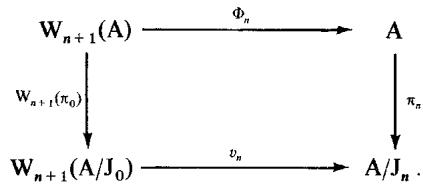
\includegraphics[keepaspectratio]{images/part002_309b7be5.jpg}}

\begin{enumerate}
\def\labelenumi{\alph{enumi})}
\setcounter{enumi}{2}
\tightlist
\item
  Set \(u_n = v_n \circ \mathbf{W}_{n+1}(\overline{\varphi}) \circ \mathbf{F}^{-n}\) Then, for every \(n \in \mathbf{N}\) , the following diagram, where the vertical arrows denote the canonical projections, is commutative
\end{enumerate}

\pandocbounded{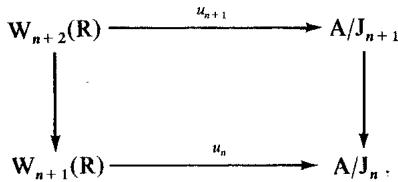
\includegraphics[keepaspectratio]{images/part002_feb0ecf4.jpg}}

\begin{enumerate}
\def\labelenumi{\alph{enumi})}
\setcounter{enumi}{3}
\tightlist
\item
  There exists a unique ring homomorphism u making the following diagram commutative.
\end{enumerate}

\pandocbounded{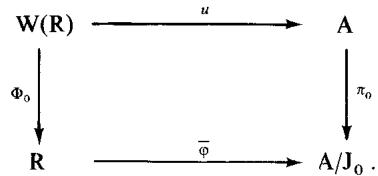
\includegraphics[keepaspectratio]{images/part002_890d1cac.jpg}}

  The homomorphism \(u\) is continuous when \(\mathbf{W}(\mathbf{R})\) is equipped with the \(p\)-adic topology, and for every \(\boldsymbol{a} = (a_n)_{n \in \mathbb{N}} \in \mathbf{W}(\mathbf{R})\), one has \(u(\boldsymbol{a}) = \sum_{n=0}^{\infty} p^n \varphi(a_n^{p^{-n}})\).

(The existence of \(u\) follows from what precedes. To prove the uniqueness of \(u\), its continuity, and its explicit expression, use the equality \(\varphi = u \circ \tau\), where \(\varphi\) is the map from R into A constructed in a), and \(\tau: \mathrm{R} \to \mathrm{W(R)}\) is the map defined in § 1, no. 5.)

\begin{enumerate}
\def\labelenumi{\alph{enumi})}
\setcounter{enumi}{4}
\tightlist
\item
  Give another proof of th. 2 of § 2, no. 4, different from the one in the text and from that of exerc. 4, c).
\end{enumerate}

\begin{enumerate}
\def\labelenumi{\arabic{enumi})}
\setcounter{enumi}{6}
\tightlist
\item
  \begin{enumerate}
  \def\labelenumii{\alph{enumii})}
  \tightlist
  \item
    Let R be a perfect ring of characteristic p, and let R' be a ring of characteristic p. Let f be a homomorphism from R into R'. Then the homomorphism W(f): W(R) → W(R') is the unique homomorphism making the following diagram commutative.
  \end{enumerate}
\end{enumerate}

\pandocbounded{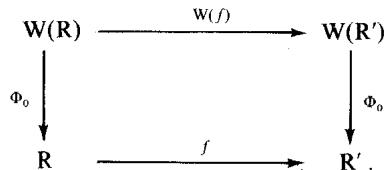
\includegraphics[keepaspectratio]{images/part002_f36acea2.jpg}}

(Use the previous exercise.)

In particular, taking \(f\) to be the p-th power map on R, prove that \(\mathrm{F}_{\mathrm{R}}\) is the unique endomorphism of \(\mathbf{W}(\mathbf{R})\) such that \(\Phi_{0} \circ \mathrm{F}_{\mathrm{R}} = f \circ \Phi_{0}\). It is characterized by the equalities

\[
\mathrm{F} _ {\mathbf {R}} (\tau (x)) = \tau (x ^ {p}) \quad \text { for all } \quad x \in \mathbf {R}  .
\]

\begin{enumerate}
\def\labelenumi{\alph{enumi})}
\setcounter{enumi}{1}
\tightlist
\item
  Let A be a ring separated and complete for the p-adic topology. Suppose that multiplication by \(p.1_{A}\) in A is injective and that A/pA is a perfect ring. Then there exists a unique endomorphism \(\sigma\) of A such that \(\sigma(x) \equiv x^{p} \mod pA\) for \(x \in A\), and the inverse of the isomorphism \(t_{\sigma}: A \to W(A/pA)\) described in exerc. 14, p.~44 is given by
\end{enumerate}

\[
(a _ {i}) _ {i \in \mathbf {N}} \mapsto \sum_ {i = 0} ^ {\infty} \varphi (a _ {i}) ^ {p ^ {- i}} p ^ {i},
\]

where \(\varphi : \mathrm{A} / p\mathrm{A} \to \mathrm{A}\) is the unique map which gives the identity of \(\mathrm{A} / p\mathrm{A}\) by passage to quotients and satisfies \(\varphi(x^p) = \varphi(x)^p\) for \(x \in \mathbb{R}\) (cf.~exerc. 6, a)).

\begin{enumerate}
\def\labelenumi{\arabic{enumi})}
\setcounter{enumi}{7}
\item
  Let C be a p-ring of infinite length, with residue field k. Every automorphism of k extends to an automorphism of C. Every automorphism of C inducing the identity on k by passage to quotients is the identity if and only if k is perfect.
\item
  Let \(k\) be a field of characteristic \(p\), \(\mathbf{C}_k\) a \(p\)-ring of infinite length and with residue field \(k\). Let A be a local ring separated and complete and \(u: \mathbf{C}_k \to \mathbf{A}\) a local homomorphism such that the homomorphism deduced from \(u\) by passage to quotients makes the residue field K of A a separable extension of \(k\). Let \(\mathbf{C}_{\mathbf{K}}\) be a \(p\)-ring of infinite length with residue field K. Prove that there exist local homomorphisms \(i: \mathbf{C}_k \to \mathbf{C}_{\mathbf{K}}\) and \(v: \mathbf{C}_{\mathbf{K}} \to \mathbf{A}\) such that \(u = v \circ i\) and that \(v\) induces the identity on K by passage to quotients.
\item
  Let \(k\) be a field of characteristic \(p\), \((\xi_{\lambda})_{\lambda \in \Lambda}\) a \(p\)-basis of \(k\), and for each integer \(n \geqslant 1\), let \(C_n\) be the subring of \(\mathbf{W}_n(k)\) generated by \(\mathbf{W}_n(k^{p^{n-1}})\) and the elements \(\tau(\xi_{\lambda}) = [\xi_{\lambda}, 0, ..., 0]\), for \(\lambda \in \Lambda\). For every integer \(n \geqslant 1\), the projection of \(\mathbf{W}_{n+1}(k)\) onto \(\mathbf{W}_n(k)\) maps \(C_{n+1}\) into \(C_n\). We denote by C the subring of \(\mathbf{W}(k)\) that is the inverse limit of the \(C_n\).
\end{enumerate}

\begin{enumerate}
\def\labelenumi{\alph{enumi})}
\item
  Let n be an integer \(\geqslant 0\). Put \(\mathbf{A} = \mathbf{W}_{n+1}(k)\) and for every integer \(i \geqslant 0\) let \(\rho_{i} = \rho_{n,i}^{A}\) be the map from k to A defined in exerc. 2, p.~69. Prove that one has, for \(a \in k\), \(\rho_{i}(a) = V^{i}\tau(a^{p^{n}})\). Deduce that the elements \(\rho_{i}(a)\) for \(a \in k\) generate the subring \(\mathbf{W}_{n+1}(k^{p^{n}})\) of A.
\item
  Let \(\tilde{\mathbf{C}}\) be a \(p\)-ring with residue field \(k\) and of infinite length, and let \((x_{\lambda})_{\lambda \in \Lambda}\) be a family of elements of \(\tilde{\mathbf{C}}\) lifting the \(p\)-basis \((\xi_{\lambda})_{\lambda \in \Lambda}\). Using exerc. 4, p.~70, prove that there exists, for each integer \(n \geqslant 1\), a unique ring homomorphism \(\varphi_n: \tilde{\mathbf{C}} \to \mathbf{W}_n(k)\) inducing the identity on \(k\) by passage to quotients, and sending \(x_{\lambda}\) onto \(\tau(\xi_{\lambda})\) for every \(\lambda \in \Lambda\). Deduce from exerc. 3, p.~69 that the image of \(\varphi_n\) is \(\mathbf{C}_n\).
\item
  The maps \((\varphi_n)_{n\geqslant 1}\) form an inverse system of maps from \(\tilde{\mathbf{C}}\) into the \(C_n\), and \(\varphi = \lim \varphi_n\) is an isomorphism from \(\tilde{\mathbf{C}}\) onto C. For each \(n\geqslant 1\), the canonical projection \(\mathbf{C}\to \mathbf{C}_n\) identifies \(C_n\) with \(\mathrm{C} / p^n\mathrm{C}\).
\end{enumerate}

\begin{enumerate}
\def\labelenumi{\arabic{enumi})}
\setcounter{enumi}{10}
\tightlist
\item
  Let \(k\) be a field of characteristic \(p\), \((\xi_{\lambda})_{\lambda \in \Lambda}\) a \(p\)-basis of \(k\), and \(C\) the Cohen subring of \(\mathrm{W}(k)\) containing \(\tau(\xi_{\lambda})\) for every \(\lambda \in \Lambda\). Let \((\varepsilon_j)_{j \in J}\) be a basis of \(k^*/(k^{*p})\) as an \(\mathbf{F}_p\)-vector space. Let \(n\) be an integer \(\geqslant 0\) and \((x_j)_{j \in J}\) be a family of elements of \(k^*\) such that the image of \(x_j\) in \(k^*/k^{*p}\) is \(\varepsilon_j\), for all \(j \in J\).
\end{enumerate}

\begin{enumerate}
\def\labelenumi{\alph{enumi})}
\item
  The group \(k^{*} / k^{*p^{n}}\) is a free \((\mathbf{Z} / p^{n}\mathbf{Z})\)-module with basis \((\overline{x}_j)_{j\in J}\), where \(\overline{x}_j\) is the class of \(x_j\) in \(k^{*} / k^{*p^{n}}\).
\item
  For every \(j \in J\), let us write the decomposition of \(x_{j}\) along the basis \((\xi^{m})_{m \in M_{n}}\) of k over \(k^{p^{n}}\) (with the notations of exerc. 3, p.~69):
\end{enumerate}

\[
x _ {j} = \sum_ {\boldsymbol {m} \in \mathbf {M} _ {n}} a _ {j, \boldsymbol {m}} ^ {p ^ {n}} \xi^ {\boldsymbol {m}}, \quad a _ {j, \boldsymbol {m}} \in k.
\]

Set

\[
\sigma_ {n} (x _ {j}) = \sum_ {m \in \mathbf {M} _ {n}} \tau (a _ {j, m} ^ {p ^ {n}} \xi^ {m}) \quad \text { for all } \quad j \in J
\]

and

\[
\sigma_ {n} (x) = \tau (x) \quad \text { for } \quad x \in k ^ {* p ^ {n}}.
\]

Then \(\sigma_{n}\) extends, in a unique way, to a multiplicative map from \(k^{*}\) into \(\mathrm{C} / p^{n + 1}\mathrm{C}\), still denoted \(\sigma_{n}\), which, by passage to quotients, determines the inclusion of \(k^{*}\) into \(k = \mathrm{C} / p\mathrm{C}\). c) Let \(\sigma_{n}^{\prime}\) be another multiplicative map from \(k^{*}\) into \(\mathrm{C} / p^{n + 1}\mathrm{C}\) defining the inclusion of \(k^{*}\) into \(k\) by passage to quotients. Then for every \(x\in k^{*}\), one has \(\sigma_{n}(x) = v(x)\sigma_{n}^{\prime}(x)\), where \(v\) is a homomorphism from \(k^{*}\) into the multiplicative group \((1 + p\mathrm{C}) / (1 + p^{n + 1}\mathrm{C})\) trivial on \(k^{*p^n}\). An arbitrary family \((\beta_j)_{j\in J}\) of elements of \(\mathrm{C} / p^n\mathrm{C}\) defines such a homomorphism by the formula

\[
v (x _ {j}) = 1 + p \beta_ {j} \quad \text { for all } \quad j \in J.
\]

\begin{enumerate}
\def\labelenumi{\alph{enumi})}
\setcounter{enumi}{3}
\item
  For every integer \(n \geqslant 0\) and every multiplicative map \(s_{n}: k^{*} \to C/p^{n+1}C\) defining the inclusion of \(k^{*}\) into k, passing to the quotient, there exists a multiplicative map \(s_{n+1}: k^{*} \to C/p^{n+2}C\) which determines \(s_{n}\) by passing to the quotient.
\item
  Prove that there exists a multiplicative section \(s:k\to C\). One can require that \(s(\xi_{\lambda})=\tau(\xi_{\lambda})\) for every \(\lambda\in\Lambda\).
\end{enumerate}

\(f)\) Let A be a local ring, separated and complete. Let \(k\) be its residue field, \((\xi_{\lambda})_{\lambda \in \Lambda}\) a \(p\)-basis of \(k\), and, for \(\lambda \in \Lambda\), let \(a_{\lambda}\) be a lifting of \(\xi_{\lambda}\) in A. Show that there exists a multiplicative section \(k^{*} \to A\) satisfying \(s(\xi_{\lambda}) = a_{\lambda}\).

\begin{enumerate}
\def\labelenumi{\arabic{enumi})}
\setcounter{enumi}{11}
\tightlist
\item
  Let A be a complete local ring whose residue field has characteristic p.
\end{enumerate}

\begin{enumerate}
\def\labelenumi{\alph{enumi})}
\item
  Let \(x \in \mathfrak{m}_{\mathrm{A}}\) . The map \(n \mapsto (1 + x)^n\) of \(\tilde{\mathbf{Z}}\) in \(1 + \mathfrak{m}_{\mathrm{A}}\) extends uniquely to a continuous map from \(\mathbf{Z}_p\) in \(1 + \mathfrak{m}_{\mathrm{A}}\) , denoted \(\alpha \mapsto (1 + x)^{\alpha}\) . This defines a structure of \(\mathbf{Z}_p\) -module on the multiplicative group \(1 + \mathfrak{m}_{\mathrm{A}}\) .
\item
  Let \(\delta\) be the formal series \(\exp\left(-\sum_{n=0}^{\infty}\mathrm{T}^{p^n}/p^n\right)\) of exercise 58, p.~68. The map \(x \mapsto \delta(x)\) from \(\mathfrak{m}_{\mathrm{A}}\) into \(1 + \mathfrak{m}_{\mathrm{A}}\) is bijective.
\item
  Let \(k\) be a perfect field of characteristic \(p\), and \(\varphi\) a local homomorphism from \(\mathbf{W}(k)\) into A. For \(\alpha \in \mathbf{W}(k)\), consider the series \(\varphi \mathrm{E}_{\mathrm{F}}(\alpha, \mathrm{T})\) obtained by applying \(\varphi\) to the coefficients of the series \(\mathrm{E}_{\mathrm{F}}(\alpha, \mathrm{T})\) from exercise 58, f), p.~68. For \(\alpha \in \mathbf{W}(k)\), \(x \in 1 + m_{\mathbf{A}}\), set \(x^{\alpha} = \varphi \mathrm{E}_{\mathrm{F}}(\alpha, \xi^{-1}(x))\). Show that this defines an action of the additive group \(\mathbf{W}(k)\) on the set \(1 + m_{\mathbf{A}}\), which extends the action of \(\mathbf{W}(\mathbf{F}_p)\) (identified with \(\mathbf{Z}_p\)) defined in a). Show that we also have, for \(a \in \mathbf{Z}_p\), \(\alpha \in \mathbf{W}(k)\), \(x \in 1 + m_{\mathbf{A}}\), the relation \((x^{\alpha})^{a} = x^{a\alpha}\).
\item
  Using exercise 15, p.~44, prove that one does not always have, for \(a \in \mathbf{Z}_{p}\), \(\alpha \in \mathbf{W}(k)\), and \(x \in 1 + m_{\mathbf{A}}\), the relation \((x^{a})^{\alpha} = x^{a\alpha}\). Nor do we always have, for \(\alpha \in \mathbf{W}(k)\) and \(x, y\) in \(1 + m_{\mathbf{A}}\), the relation \((xy)^{\alpha} = x^{\alpha}y^{\alpha}\).
\end{enumerate}

\begin{enumerate}
\def\labelenumi{\arabic{enumi})}
\setcounter{enumi}{12}
\tightlist
\item
  Let A be a complete discrete valuation ring of characteristic zero, whose residue field has characteristic \(p\). Let K be the field of fractions of A, \(\overline{\mathbf{K}}\) an algebraic closure of K, equipped with the unique valuation \(v\) extending that of K (VI, § 8, no. 7), \(\hat{\mathbf{K}}\) the completion of \(\overline{\mathbf{K}}\), \(\hat{\mathbf{A}}\) the valuation ring of \(\hat{\mathbf{K}}\). Put \(e = v(p)\).
\end{enumerate}

\begin{enumerate}
\def\labelenumi{\alph{enumi})}
\tightlist
\item
  The series \(\log(1 + x) = \sum_{i=1}^{\infty} (-1)^{i-1} x^i / i\) converges for \(v(x) > 0\) and defines homomorphisms of \(\mathbf{Z}_p\)-modules (cf. exerc. 12).
\end{enumerate}

\[
\begin{array}{l} \log : 1 + \mathfrak {m} _ {\hat {\mathbf {A}}} \to \hat {\mathbf {K}}, \\ \log : 1 + \mathfrak {m} _ {\mathbf {A}} \to \mathbf {K}. \end{array}
\]

\begin{enumerate}
\def\labelenumi{\alph{enumi})}
\setcounter{enumi}{1}
\tightlist
\item
  The series \(\exp(x) = \sum_{i=0}^{\infty} x^{i}/i!\) converges on the ideal \(a\) of \(\hat{K}\) consisting of elements of valuation \(>e/(p-1)\), and defines homomorphisms of \(\mathbf{Z}_{p}\)-modules
\end{enumerate}

\[
\begin{array}{l} \exp : a \to 1 + m _ {\hat {A}} \\ \exp : a \cap K \to 1 + m _ {A}. \end{array}
\]

\begin{enumerate}
\def\labelenumi{\alph{enumi})}
\setcounter{enumi}{2}
\tightlist
\item
  For \(x \in \mathfrak{a}\), one has \(\log(\exp(x)) = x\), \(\log(1 + x) \in \mathfrak{a}\), and \(\exp(\log(1 + x)) = 1 + x\). Thus exp defines isomorphisms of \(\mathbf{Z}_p\)-modules
\end{enumerate}

\[
\begin{array}{l}\mathfrak {a} \rightarrow 1 + \mathfrak {a}\\\mathfrak {a} \cap \mathbf {K} \rightarrow 1 + (\mathfrak {a} \cap \mathbf {K})\end{array}
\]

with inverses defined by log.

\begin{enumerate}
\def\labelenumi{\alph{enumi})}
\setcounter{enumi}{3}
\tightlist
\item
  The kernel of log on \(1 + m_{\hat{A}}\) consists of the roots of unity whose order is a power of p. The image \(\log(1 + m_{\hat{A}})\) is equal to \(m_{\hat{A}}\).
\end{enumerate}

\begin{enumerate}
\def\labelenumi{\arabic{enumi})}
\setcounter{enumi}{13}
\tightlist
\item
  Let A be a complete discrete valuation ring of characteristic zero, whose residue field \(k\) is perfect of characteristic \(p\). Let K be the field of fractions of A. Let \(n\) be an integer \(\geqslant 1\) and \(\zeta\) a primitive \(p^n\)-th root of unity in K. Let \(\overline{\mathbf{K}}\) be an algebraic closure of K, equipped with the unique valuation \(v\) extending that of K.
\end{enumerate}

\begin{enumerate}
\def\labelenumi{\alph{enumi})}
\item
  Let C be the Cohen subring of A, and T its field of fractions; this is a subfield of K. The canonical isomorphism from W(k) to C induces an isomorphism from \(W(k) \otimes_{\mathbb{Z}} \mathbb{Q}\) to T. For every finite extension l of k, the field \(W(l) \otimes_{\mathbb{Z}} \mathbb{Q}\) is a finite extension of \(W(k) \otimes_{\mathbb{Z}} \mathbb{Q}\), Galois if l is. If l is Galois, the unique extension \((T_l)\) of T in \(\overline{\mathbf{K}}\) isomorphic to \(W(l) \otimes_{\mathbb{Z}} \mathbb{Q}\) has residue field isomorphic to l. In particular, the field \(T_{\infty}\), the union of the fields \((T_l)\) as l ranges over the finite Galois extensions of k (in a fixed algebraic closure of k), has as its residue field an algebraic closure \(\overline{k}\) of k. The same holds for K. For each extension l of k in \(\overline{k}\), we denote by \((T_l)\) the unique extension of T in \(T_{\infty}\) whose residue field is the subfield l of \(\overline{k}\), and by \((K_l)\) the compositum of K and \((T_l)\). Then, if l is Galois over k, \((K_l)\) is Galois over K and its Galois group is canonically identified with the Galois group of l over k.
\item
  Let \(k_n\) be the largest abelian extension of \(k\) in \(\overline{k}\) whose Galois group is annihilated by \(p^n\). By virtue of Exercise 19, p.~45, we have a canonical isomorphism
\end{enumerate}

\[
\operatorname{Gal} (k _ {n} / k) \to \operatorname{Hom} (\mathrm{W} _ {n} (k) / \wp \mathrm{W} _ {n} (k), \mathbf {Z} / p ^ {n} \mathbf {Z}).
\]

By A, V, p.~85, th. 4, we have a canonical isomorphism

\[
\operatorname{Gal} \left(\mathrm{K} _ {k _ {n}} / \mathrm{K}\right)\rightarrow \operatorname{Hom} \left(\mathrm{H} _ {n} / \mathrm{K} ^ {* p ^ {n}}, \mu_ {p _ {n}} (\mathrm{K})\right)
\]

\(\text{where }\mathbf{H}_n = (\mathbf{K}_{\overline{k}}^*)^{p^n}\cap \mathbf{K}^*\)

Prove that there exists a unique mapping

\[
\mathrm{E} ^ {*}: \mathrm{W} _ {n} (k) / \wp \mathrm{W} _ {n} (k) \rightarrow \mathrm{H} _ {n} / \mathrm{K} ^ {* p ^ {n}}
\]

such that the following diagram is commutative:

\[
\begin{array}{c} \operatorname{Gal} (K _ {k _ {n}} / K) \xrightarrow {} \operatorname{Hom} (H _ {n} / K ^ {* p ^ {n}}, \mu_ {p ^ {n}} (K)) \\ \Bigg \downarrow \\ \operatorname{Gal} (k _ {n} / k) \xrightarrow {} \operatorname{Hom} (W _ {n} (k) / \wp W _ {n} (k), Z / p ^ {n} Z), \end{array}
\]

where the vertical arrow on the right denotes the map which, to the homomorphism \(\varphi\) of \(\mathbf{H}_n / \mathbf{K}^{*p^n}\) into \(\mu_{p^n}(\mathbf{K})\), associates the homomorphism \(\psi\) of \(\mathrm{W}_n(k) / \wp\mathrm{W}_n(k)\) into \(\mathbf{Z} / p^n\mathbf{Z}\) defined by \(\zeta^{\psi (\alpha)} = \varphi (\mathrm{E}^{*}(\alpha))\) for \(\alpha \in \mathrm{W}_n(k) / \wp\mathrm{W}_n(k)\). The map \(\mathrm{E}^*\) is an isomorphism.

\begin{enumerate}
\def\labelenumi{\arabic{enumi})}
\setcounter{enumi}{14}
\tightlist
\item
  Let us keep the hypotheses and notations of the preceding exercise.
\end{enumerate}

\begin{enumerate}
\def\labelenumi{\alph{enumi})}
\tightlist
\item
  Let \(\alpha \in \mathbf{W}(k)\) and \(\overline{\alpha} \in \mathbf{W}(\overline{k})\) be such that \(p(\overline{\alpha}) = \alpha\) (cf. p. 45, exerc. 19). Then the element \(\zeta^{p^{n\overline{\alpha}}}\) (p.~72, exerc. 12) of the completion \(\widehat{\mathbf{K}}\) of \(\overline{\mathbf{K}}\) depends only on \(\alpha\), belongs to \(\mathbf{K}\), and we have
\end{enumerate}

\[
v \left(\zeta^ {p ^ {n} \bar {\alpha}} - 1\right) \geqslant e p / (p - 1) \quad (\text { with } e = v (p)).
\]

(One may prove the equality

\[
\log \left(\zeta^ {p ^ {n} \overline {{{\alpha}}}}\right) = - p ^ {n} \sum_ {j = 1} ^ {\infty} \sum_ {\sigma = 0} ^ {j - 1} \left(\mathrm{F} ^ {\sigma} \alpha\right) \frac {\pi^ {p ^ {j}}}{p ^ {j}}
\]

\(\text{where }\pi = \delta^{-1}(\zeta)\) (loc. cit.) and where F denotes the Frobenius automorphism of \(\mathbf{W}(k)\).)

\begin{enumerate}
\def\labelenumi{\alph{enumi})}
\setcounter{enumi}{1}
\tightlist
\item
  For \(\alpha \in \mathbf{W}(k)\), denote by \(\mathrm{E}^{**}(\alpha)\) the class in \(\mathrm{K}^* / \mathrm{K}^{*p^n}\) of \(\zeta^{p^n\overline{\alpha}}\). Then \(\mathrm{E}^{**}(\alpha)\) equals 1 if \(\alpha \in p\mathbf{W}(k)\) or if \(\alpha \in p^n\mathbf{W}(k)\). The map from \(\mathrm{W}_n(k)/\wp\mathrm{W}_n(k)\) into \(\mathrm{K}^* / \mathrm{K}^{*p^n}\) which associates to the class of \(\alpha \in \mathbf{W}(k)\) the element \(\mathrm{E}^{**}(\alpha)\) takes its values in \(\mathrm{H}_n / (\mathrm{K}^*)^{p^n}\) and satisfies the conditions of exercise 14, b).
\end{enumerate}

\begin{enumerate}
\def\labelenumi{\arabic{enumi})}
\setcounter{enumi}{15}
\tightlist
\item
  Let A be a complete discrete valuation ring with residue field k.
\end{enumerate}

\begin{enumerate}
\def\labelenumi{\alph{enumi})}
\item
  Prove that there exists a multiplicative section \(\varphi:k^{*}\to\mathring{\mathrm{A}}\) (If A contains a field, use § 3. Otherwise, use exerc. 11, p.~72.)
\item
  Let \(t\) a uniformizer of A, \(\mathcal{C}\) the group generated by \(t\) , and \(\varphi:k^{*}\to A\) a multiplicative section. The multiplicative group of the field of fractions of A decomposes as a direct product. \(\mathcal{C}\times\varphi(k^{*})\times(1+\mathfrak{m}_{\mathbf{A}})\) .
\item
  Suppose A has equal characteristics and let K be a coefficient field. Then A is identified with the ring K{[}{[}T{]}{]} formal series with coefficients in K, and the group 1 + m\_A is identified with the group \(\Lambda(K) = 1 + TK[[T]]\) (cf. p. 56, exerc. 42). If K has characteristic zero, the map \(\varphi \mapsto \frac{1}{T} \log \varphi\) of the group \(\Lambda(K)\) in the additive group \(K[[T]]\) is an isomorphism. If A has characteristic \(p, 1 + m_A\) is identified with the group \(W(A)^L\) where L is the set of positive integers coprime to \(p\) (using Exercises 40, \(h\) ) p.~54 and 43, \(b\) ), p.~57).
\end{enumerate}

\begin{enumerate}
\def\labelenumi{\arabic{enumi})}
\setcounter{enumi}{16}
\tightlist
\item
  Let A be a complete discrete valuation ring whose residue field k is perfect of characteristic p and whose fraction field is of characteristic 0. Let f be the unique homomorphism from W(k) to A that induces the identity on the residue field k. Finally, let π be a uniformizer of A.
\end{enumerate}

\begin{enumerate}
\def\labelenumi{\alph{enumi})}
\item
  There exists an Eisenstein polynomial P with coefficients in \(f(\mathbf{W}(k))\) such that \(\mathbf{P}(\pi)=0\) (use VIII, § 5, no. 4).
\item
  Let \(e\) be the valuation of \(p\). For every integer \(n \geqslant 0\), denote by \(U_n\) the multiplicative group \(1 + m_A^n\), and set \(\lambda(n) = \inf(np, n + e)\), \(e_1 = e/(p - 1)\). Let \(u\) be the class in \(k^*\) of \(p\pi^{-e}\). Let \(\varphi\) be the endomorphism of \(U_1\) which sends \(x\) to \(x^p\). We then have, for every integer \(n \geqslant 1\), \(\varphi(U_n) \subset U_{\lambda(n)}\), \(\varphi(U_{n+1}) \subset U_{\lambda(n)+1}\), and the induced homomorphism \(\varphi_n: U_n/U_{n+1} \to U_{\lambda(n)}/U_{\lambda(n)+1}\) is an isomorphism if \(n \neq e_1\). If \(n = e_1\), \(\varphi_n\) is injective if and only if the equation \(x^{p-1} + u = 0\) has no solution in \(k\), and surjective if and only if the equation \(x^p + ux = y\) has a solution in \(k\) for every \(y \in k\).
\item
  The following two conditions are equivalent:
\end{enumerate}

\begin{enumerate}
\def\labelenumi{(\roman{enumi})}
\item
  A contains the p-th roots of unity;
\item
  \(e_1\) is an integer and the equation \(x^{p - 1} + u = 0\) has a solution in \(k\) .
\end{enumerate}

\begin{enumerate}
\def\labelenumi{\alph{enumi})}
\setcounter{enumi}{3}
\item
  The topology induced on \(\mathbf{U}_1\) by that of A coincides with the p-adic topology of \(\mathbf{U}_1\).
\item
  Let S be the set of integers \(n \geqslant 1\) such that A contains the \(p^n\)-th roots of unity. Then \(s = \text{Card}(S)\) is finite.
\item
  Let I be the set of integers \(i\) coprime to \(p\) and satisfying \(1 \leqslant i < e + e_1\). Then we have Card(I) = \(e\), and the image of \(\mathbf{N} - \{0\}\) by \(\lambda\) is \(\mathbf{N} - (\mathbf{I} \cup \{0\})\).
\item
  If \(e_1\) is an integer and \(\varphi_{e_1}\) is not surjective, set \(\mathbf{I}' = \mathbf{I} \cup \{e + e_1\}\); otherwise, set \(\mathbf{I}' = \mathbf{I}\). For each integer \(i \in \mathbf{I}'\), let \(\pi_i\) be an element of A with valuation \(i\). Then the map from \(\mathbf{W}(k)^{\mathbf{I}'}\) into \(\mathbf{U}_1\) which sends \((a_i)_{i \in \mathbf{I}'}\) to \(\prod_{i \in \mathbf{I}'} (1 + \pi_i)^{a_i}\) is surjective; it is a homomorphism of
\end{enumerate}

\(\mathbf{Z}_{p}\)-modules.

\(h)\) Let \(n\) be an integer \(>e_{1}\) and \(\mathbf{I}(n)\) the interval \([n, \lambda(n) - 1]\) of \(\mathbf{N}\). For every integer \(i \in \mathbf{I}(n)\), let \(\pi_{i}\) be an element of \(\mathbf{A}\) of valuation \(i\). Then the map from \(\mathbf{W}(k)^{\mathbf{I}(n)}\) into \(\mathbf{U}_{n}\) which sends \((a_{i})_{i \in \mathbf{I}(n)}\) to \(\prod_{i \in \mathbf{I}(n)} (1 + \pi_{i})^{a_{i}}\) is an isomorphism of \(\mathbf{Z}_{p}\)-modules.

\begin{enumerate}
\def\labelenumi{\roman{enumi})}
\tightlist
\item
  Suppose that \(k\) is finite and denote by \(d\) the degree over \(\mathbf{Q}_{p}\) of the field of fractions of A. Then the \(\mathbf{Z}_{p}\)-module \(1 + m_{\mathbf{A}}\) is isomorphic to \((\mathbf{Z}/p^{s}\mathbf{Z}) \times \mathbf{Z}_{p}^{d}\) (One may use the preceding questions, or else use Exercise 13, p.~73.)
\end{enumerate}

\exercisesection{FIELDS OF REPRESENTATIVES}

\begin{enumerate}
\def\labelenumi{\arabic{enumi})}
\tightlist
\item
  Let \(p\) be a prime number, \(G\) the free group on two generators \(X\) and \(Y\), and \(F_p[G]\) the group algebra of \(G\) over \(F_p\). Set \(Z = XY - YX\) and denote by \(\mathfrak{a}\) the two-sided ideal of \(F_p[G]\) generated by the elements \(ZX - XZ\), \(ZY - YZ\), and \(Z^2\). Put \(A = F_p[G]/\mathfrak{a}\), and denote by \(\mathfrak{z}\) the two-sided ideal of \(A\) generated by the image of \(Z\) in \(A\) (we will still denote by \(X\), \(Y\), \(Z\) the images in \(A\) of \(X\), \(Y\), and \(Z\)). a) Let \(a\) be an element of \(A\). Prove that there exist two finitely supported families of elements of \(F_p\), namely \((p_{\alpha,\beta})_{(\alpha,\beta)\in\mathbf{Z}^2}\) and \((q_{\alpha,\beta})_{(\alpha,\beta)\in\mathbf{Z}^2}\), uniquely determined by the condition
\end{enumerate}

\[
a = \sum_ {(\alpha , \beta) \in \mathbf {Z} ^ {2}} (p _ {\alpha , \beta} + q _ {\alpha , \beta} \mathbf {Z}) \mathrm{X} ^ {\alpha} \mathrm{Y} ^ {\beta}.
\]

Deduce that the quotient algebra \(A/\mathfrak{z}\) is commutative and integral, and that the ideal \(\mathfrak{z}\) is contained in the center of A.

\begin{enumerate}
\def\labelenumi{\alph{enumi})}
\setcounter{enumi}{1}
\tightlist
\item
  For every pair \((a, b)\) of elements of A, there exists an element c of A such that
\end{enumerate}

\[
  a ^ {k} b - b a ^ {k} = k a ^ {k - 1} c Z \quad \text { for every integer } k \geqslant 0.
\]

From this, deduce that the set \(A^{p}\) of the p-th powers of the elements of A is contained in the center of A.

\begin{enumerate}
\def\labelenumi{\alph{enumi})}
\setcounter{enumi}{2}
\tightlist
\item
  The multiplicative part \(S = A - \mathfrak{z}\) of \(A\) allows a computation of fractions on the right and on the left (II, § 2, exerc. 22). We denote by B the ring of fractions of \(A\) thus constructed.
\end{enumerate}

(To verify, for example, that for every \(a\) in A and every \(s\) in S, there exists \(b \in A\) and \(t \in S\) such that \(at = sb\), take \(b = s^{p-1}a\), \(t = s^p\), and use b).)

\begin{enumerate}
\def\labelenumi{\alph{enumi})}
\setcounter{enumi}{3}
\item
  Prove that the canonical map from A to B is injective. (Note that the kernel of this map is contained in \(\mathfrak{z}\), and reason as in (a)).
\item
  The center of B contains Z. If m is the two-sided ideal of B generated by Z, then \(m^{2} = 0\).
\item
  The ideal m is the set of non-invertible elements of B, and the field B/m is isomorphic to the field \(\mathbf{F}_{p}(\mathbf{X}, \mathbf{Y})\) .
\item
  Prove that there is no subfield of B whose image in B/m is all of B/m.
\end{enumerate}

In Exercises 2 to 5, the (commutative) topological rings are assumed to be linearly topologized. If A and B are two topological rings and B is an A-algebra, one says that B is a topological A-algebra if the homomorphism from A to B defining the algebra structure is continuous.

\begin{enumerate}
\def\labelenumi{\arabic{enumi})}
\setcounter{enumi}{1}
\tightlist
\item
  Let A be a topological ring, and let B be a topological A-algebra. We say that B is a formally smooth A-algebra \(^{1}\) if, for every discrete topological A-algebra C, every ideal j of C with square zero, and every continuous A-homomorphism \(u: B \to C/j\) there exists a continuous A-homomorphism \(v: B \to C\) which, by passing to the quotient, induces u.
\end{enumerate}

Let A be a ring, and B an A-algebra. We say that B is a smooth A-algebra if B is a formally smooth A-algebra when A and B are endowed with the discrete topologies.

\begin{enumerate}
\def\labelenumi{\alph{enumi})}
\item
  Let A be a topological ring and B a formally smooth A-algebra. Let C be a ring and j an ideal of C. Endow C with the j-adic topology, and suppose C is separated and complete for this topology. Then, for every continuous A-homomorphism \(u:B\to C/\mathfrak{j}\), there exists a continuous A-homomorphism \(v:B\to C\) which, by passing to the quotient, induces \(u\).
\item
  Let A be a ring. Every polynomial algebra over A is a smooth A-algebra.
\item
  Let A be a topological ring. If B is a formally smooth A-algebra and C is a formally smooth B-algebra, then C is a formally smooth A-algebra.
\item
  Let A be a topological ring, B a formally smooth A-algebra, and A' a topological A-algebra. Then the topological A'-algebra \(B \otimes_{A} A'\) (III, § 2, exerc. 28) is a formally smooth A'-algebra.
\item
  Let A be a topological ring, and let B be a formally smooth A-algebra. Let S (resp. T) be a multiplicative subset of A (resp. B) such that the image of S in B is contained in T. Then \(T^{-1}B\) is a formally smooth \(S^{-1}A\)-algebra (see III, § 2, exerc. 27 for the topology of \(T^{-1}B\) and \(S^{-1}A\)).
\item
  Let n be an integer \(\geqslant 1\), and let \((\mathbf{B}_{i})_{1\leqslant i\leqslant n}\) be a family of topological A-algebras. For \(\prod_{i=1}^{n} B_{i}\) to be a formally smooth A-algebra, it is necessary and sufficient that \(B_{i}\) be a formally smooth A-algebra for \(1 \leqslant i \leqslant n\).
\item
  Let A be a topological ring, B a topological A-algebra, \(\hat{A}\) and \(\hat{B}\) the respective separated completions of A and B. Then the following three conditions are equivalent:
\end{enumerate}

\begin{enumerate}
\def\labelenumi{(\roman{enumi})}
\item
  B is a formally smooth A-algebra;
\item
  \(\hat{\mathbf{B}}\) is a formally smooth A-algebra;
\item
  \(\hat{\mathbf{B}}\) is a formally smooth \(\hat{\mathbf{A}}\)-algebra.
\end{enumerate}

\(h)\) We resume the notation and hypotheses of \(e\)). Then \(\mathbf{B}\{\mathrm{T}^{-1}\}\) is a formally smooth \(\mathbf{A}\{\mathrm{S}^{-1}\}\)-algebra.

\begin{enumerate}
\def\labelenumi{\arabic{enumi})}
\setcounter{enumi}{2}
\tightlist
\item
  Let \(k\) be a field and A a commutative \(k\)-algebra. For every integer \(i \geqslant 1\), set \(\mathbf{B}_i = \underbrace{\mathbf{A} \otimes_k \mathbf{A} \otimes_k \cdots \otimes_k \mathbf{A}}_{i \text{ terms}}\) and endow \(\mathbf{B}_i\) with the structure of an A-algebra obtained by letting
\end{enumerate}

A acts on the first component. Set \(C_{1} = B_{2}\), \(C_{2} = B_{3}\), \(C_{3} = B_{4} \oplus B_{3}\), and define A-linear maps \(d_{2}:C_{2} \to C_{1}\) and \(d_{3}:C_{3} \to C_{2}\) by the formulas

\[
d _ {3} ((1 \otimes x \otimes y \otimes z, 1 \otimes \alpha \otimes \beta)) = x \otimes y \otimes z - 1 \otimes x y \otimes z + 1 \otimes x \otimes y z - z \otimes x \otimes y + 1 \otimes \alpha \otimes \beta - 1 \otimes \beta \otimes \alpha,
\]

\[
d _ {2} (1 \otimes \alpha \otimes \beta) = \alpha \otimes \beta - 1 \otimes \alpha \beta + \beta \otimes \alpha ,
\]

\(^{1}\) If A is a local, Noetherian, complete algebra over a (discrete) field k, this definition coincides with that given in VIII, p.~98, exerc. 30, according to exerc. 5 below.

for any choice of elements \(x, y, z, \alpha, \beta\) of A. One thus obtains a complex of A-modules

\[
\mathrm{C} _ {k} (\mathrm{A}): \mathrm{C} _ {3} \xrightarrow {d _ {3}} \mathrm{C} _ {2} \xrightarrow {d _ {2}} \mathrm{C} _ {1}.
\]

If N is an A-module, one says that a \(k\)-bilinear map \(f: \mathbf{A} \times \mathbf{A} \to \mathbf{N}\) is a 2-cocycle if one has the identity \(xf(y, z) - f(xy, z) + f(x, yz) - zf(x, y) = 0\) for \(x, y, z\) in A, and that it is symmetric if one has \(f(x, y) = f(y, x)\) for every pair \((x, y) \in \mathbf{A} \times \mathbf{A}\).

\begin{enumerate}
\def\labelenumi{\alph{enumi})}
\tightlist
\item
  The following conditions are equivalent:
\end{enumerate}

\begin{enumerate}
\def\labelenumi{(\roman{enumi})}
\item
  the complex \(\operatorname{Hom}_{\mathbf{A}}(\mathbf{C}_k(\mathbf{A}), \mathbf{N})\) is acyclic for every A-module \(\mathbf{N}\) ;
\item
  for every A-module N, every symmetric 2-cocycle \(f:A\times A\to\mathbf{N}\) is a 1-coboundary, that is, of the form \(f(a,b)=ag(b)+bg(a)-g(ab)\) with \(g\in\mathrm{Hom}_{k}(\mathbf{A},\mathbf{N})\);
\item
  A is a smooth algebra over k.
\end{enumerate}

\begin{enumerate}
\def\labelenumi{\alph{enumi})}
\setcounter{enumi}{1}
\tightlist
\item
  If A is a field, the preceding conditions are also equivalent to the condition that the complex \(C_{k}(A)\) be acyclic.
\end{enumerate}

\begin{enumerate}
\def\labelenumi{\arabic{enumi})}
\setcounter{enumi}{3}
\tightlist
\item
  \begin{enumerate}
  \def\labelenumii{\alph{enumii})}
  \tightlist
  \item
    Let \(k\) be a field and \(K\) an extension of \(k\). If \(K\) is separable over \(k\), then \(K\) is a smooth \(k\)-algebra. (If \(K\) is a finitely generated extension of \(k\), use prop. 1 of § 3, n° 2. In the general case, write \(K\) as a union of finitely generated extensions of \(k\) and use the preceding exercise.)
  \end{enumerate}
\end{enumerate}

\begin{enumerate}
\def\labelenumi{\alph{enumi})}
\setcounter{enumi}{1}
\tightlist
\item
  Let A be a local ring that is separated and complete, containing a field k. Using a), prove that A possesses a field of representatives. If the residue field of A is a separable extension of k, then A possesses a field of representatives containing k.
\end{enumerate}

\begin{enumerate}
\def\labelenumi{\arabic{enumi})}
\setcounter{enumi}{4}
\tightlist
\item
  Let A be a Noetherian local ring containing a field \(k\) and m the maximal ideal of A. We assume that A is a formally smooth \(k\)-algebra (the field \(k\) being discrete).
\end{enumerate}

\begin{enumerate}
\def\labelenumi{\alph{enumi})}
\item
  Let K be a field of representatives of the ring \(\mathbb{A}/\mathfrak{m}^2\) (exercise 4, b)), and let \(x_1, \ldots, x_d\) be elements of m whose images form a basis of the K-vector space \(\mathfrak{m}/\mathfrak{m}^2\). Let \(\mathrm{K}[\mathrm{X}_1, \ldots, \mathrm{X}_d]\) be the ring of polynomials in \(d\) variables \(\mathrm{X}_1, \ldots, \mathrm{X}_d\), let \(\mathfrak{n}\) be its ideal generated by \(\mathrm{X}_1, \ldots, \mathrm{X}_d\), and let \(\varphi\) be the homomorphism from \(\mathrm{K}[\mathrm{X}_1, \ldots, \mathrm{X}_d]\) into \(\mathbb{A}/\mathfrak{m}^2\) which sends \(\mathrm{X}_i\) to \(x_i\) for \(1 \leqslant i \leqslant d\) and induces the identity on K. Then \(\varphi\) induces an isomorphism \(\overline{\varphi}\) from \(\mathrm{K}[\mathrm{X}_1, \ldots, \mathrm{X}_d]/\mathfrak{n}^2\) onto \(\mathbb{A}/\mathfrak{m}^2\).
\item
  For every integer \(n \geqslant 1\), there exists a homomorphism \(\psi_n: \mathbb{A} \to \mathrm{K}[\mathrm{X}_1, \ldots, \mathrm{X}_d]/\mathfrak{n}^{n+1}\) which, by passage to quotients, induces \(\overline{\varphi}^{-1}\). Such a homomorphism \(\psi_n\) is surjective.
\item
  For every integer \(n \geqslant 1\), the length of the A-module \(\mathbf{A} / \mathfrak{m}^{n+1}\) is at least \(\binom{d+n}{d}\), and one has \(\dim(\mathbf{A}) \geqslant d\).
\item
  For every finite extension \(k'\) of \(k\), and every maximal ideal \(m'\) of the semi-local ring \(A \otimes_k k'\), the local ring \((A \otimes_k k')_{m'}\) is regular.
\end{enumerate}

\begin{enumerate}
\def\labelenumi{\arabic{enumi})}
\setcounter{enumi}{5}
\tightlist
\item
  Let \(k\) be a field and \(K\) an extension of \(k\). Assume that \(K\) is a smooth \(k\)-algebra. Let \(k'\) be an algebraic extension of finite degree of \(k\).
\end{enumerate}

\begin{enumerate}
\def\labelenumi{\alph{enumi})}
\item
  The ring K \(\otimes_{k} k'\) is a product of a finite number of Artinian local rings, which are smooth \(k'\)-algebras (use exerc. 2, p.~76).
\item
  The ring K \(\otimes_{k} k'\) is reduced (use the preceding exercise).
\item
  The field K is separable over k.
\end{enumerate}

\begin{enumerate}
\def\labelenumi{\arabic{enumi})}
\setcounter{enumi}{6}
\tightlist
\item
  Let \(k\) be a field, \(P\) its prime subfield, and \(K\) an extension of \(k\). Then the following conditions are equivalent:
\end{enumerate}

\begin{enumerate}
\def\labelenumi{\alph{enumi})}
\item
  Every derivation of k into a K-module M extends uniquely to a derivation of K into M.
\item
  We have \(\Omega_{\mathbf{P}}(\mathbf{K}) = \Omega_{\mathbf{P}}(k)\otimes_k\mathbf{K}\).
\item
  The field K is separable over k, and \(\Omega_{k}(\mathbf{K}) = 0\) .
\end{enumerate}

If \(k\) is of characteristic 0, these conditions are also equivalent to the condition:

\begin{enumerate}
\def\labelenumi{\alph{enumi})}
\setcounter{enumi}{3}
\tightlist
\item
  The field K is an algebraic extension of k.
\end{enumerate}

If \(k\) has characteristic \(p\ne0\), they are also equivalent to the conditions:

\begin{enumerate}
\def\labelenumi{\alph{enumi})}
\setcounter{enumi}{4}
\item
  \(\mathbf{K} = k\otimes_{k^p}\mathbf{K}^p.\)
\item
  Every p-basis of k is also a p-basis of K.
\end{enumerate}

\begin{enumerate}
\def\labelenumi{\arabic{enumi})}
\setcounter{enumi}{7}
\tightlist
\item
  Let \(k\) be a field and \(K\) an extension of \(k\). We say that \(K\) is formally étale over \(k\) if, for every \(k\)-algebra \(A\), every ideal \(a\) of \(A\) with square zero, and every \(k\)-homomorphism \(u:K\to A/a\), there exists a unique \(k\)-homomorphism \(v:K\to A\) which gives \(u\) by passing to the quotient.
\end{enumerate}

\begin{enumerate}
\def\labelenumi{\alph{enumi})}
\item
  If K is formally étale over k, the equivalent conditions of the preceding exercise are satisfied. (If M is a K-module, consider the k-algebra whose underlying k-vector space is K ⊕ M, with M being an ideal of square zero.)
\item
  Conversely, if the equivalent conditions of the preceding exercise are satisfied, then K is formally étale over k. (Since the field K is separable over k, Exercise 4 allows one to prove the existence of v.)
\item
  Let \(\mathbf{B} = (b_{i})_{i\in\mathbf{I}}\) be a family of elements of K such that \((db_{i})_{i\in\mathbf{I}}\) is a basis of \(\Omega_{k}(\mathbf{K})\) over K. If K is separable over k, then \(k(\mathbf{B})\) is a purely transcendental extension of k (use Th. 2 of A, V, p.~125, Th. 1 of A, V, p.~97, and Exerc. 6 of A, V, p.~165) and K is formally étale over \(k(\mathbf{B})\).
\end{enumerate}

\begin{enumerate}
\def\labelenumi{\arabic{enumi})}
\setcounter{enumi}{8}
\tightlist
\item
  Let A be a local ring of equal characteristics, \(m_{A}\) its maximal ideal, and k a subfield of A. Then the residue field \(\kappa_{A}\) is a k-algebra. One says that k is a weak residue field of A if \(\kappa_{A}\) is formally étale over k (exerc. 8).
\end{enumerate}

\begin{enumerate}
\def\labelenumi{\alph{enumi})}
\item
  If A has a field of weak representatives \(k\), then the separated completion \(\hat{\mathbf{A}}\) of A has a unique field of representatives containing the image of \(k\) in \(\hat{\mathbf{A}}\).
\item
  Let B be a local ring contained in A, with maximal ideal \(m_{B} = m_{A} \cap B\). If \(\kappa_{A}\) is a separable extension of the residue field \(\kappa_{B}\) of B, every weak residue field of B is contained in a weak residue field of A (use Exercise 8(c)).
\item
  Let B be a local ring contained in A, with maximal ideal \(m_{B} = m_{A} \cap B\). Suppose further that A has characteristic \(p\ne0\) and contains \(B^{p}\). Then there exists a weak field of representatives of A which contains a weak field of representatives of B.
\end{enumerate}
% semantic-fragments: legacy-input-seam
\relax{}
\exercisesection{INTEGRAL CLOSURE OF A COMPLETE LOCAL RING}

\begin{enumerate}
\def\labelenumi{\arabic{enumi})}
\tightlist
\item
  Let A be a semi-local Noetherian integral domain of dimension 1.
\end{enumerate}

\begin{enumerate}
\def\labelenumi{\alph{enumi})}
\item
  The integral closure of A is a finite A-algebra if and only if the completion \(\hat{\mathbf{A}}\) of A is reduced. (If \(\hat{\mathbf{A}}\) is reduced, use the corollary of Theorem 2 of § 4, No. 2. For the converse implication, reduce to the case where A is integrally closed, and argue as in the proof of Theorem 3 of § 4, No. 4).
\item
  The following three conditions are equivalent:
\end{enumerate}

\begin{enumerate}
\def\labelenumi{(\roman{enumi})}
\item
  A is a Japanese ring;
\item
  A is a Nagata ring;
\item
  \(\hat{\mathbf{A}}\) is reduced and if \(q_{1},\ldots,q_{n}\) are the minimal prime ideals of \(\hat{\mathbf{A}}\) then the fields \(\kappa(q_{i})\) are separable extensions of the field of fractions of A.
\end{enumerate}

\begin{enumerate}
\def\labelenumi{\arabic{enumi})}
\setcounter{enumi}{1}
\tightlist
\item
  Let A be a Noetherian local ring of dimension 1. Then the following conditions are equivalent:
\end{enumerate}

\begin{enumerate}
\def\labelenumi{\alph{enumi})}
\item
  A is regular;
\item
  A is integrally closed;
\item
  A is a discrete valuation ring.
\end{enumerate}

\begin{enumerate}
\def\labelenumi{\arabic{enumi})}
\setcounter{enumi}{2}
\tightlist
\item
  A ring A is said to be normal if the ring \(\mathbf{A}_{\mathfrak{p}}\) is integrally closed for every prime ideal p of A.
\end{enumerate}

\begin{enumerate}
\def\labelenumi{\alph{enumi})}
\item
  A normal ring A is reduced, and every prime ideal p of A contains exactly one minimal prime ideal of A. For every minimal prime ideal p of A, the ring A/p is integrally closed.
\item
  A Noetherian normal ring A is isomorphic to a finite product of integrally closed Noetherian rings.
\item
  Let A be a Noetherian normal ring and let a be an element of A. Then Ass \(_{A}\) (A/aA) contains no embedded prime ideal (IV, § 2, no. 3, remark).
\end{enumerate}

\begin{enumerate}
\def\labelenumi{\arabic{enumi})}
\setcounter{enumi}{3}
\tightlist
\item
  Let A be a ring. We consider the following two conditions on A:
\end{enumerate}

(R1) For every prime ideal \(\mathfrak{p}\) of A of height ≤ 1, the ring \(A_{\mathfrak{p}}\) is regular.

(S2) The set \(\mathrm{Ass}_{\mathbf{A}}(\mathbf{A})\) and, for every cancellable element \(a\) of A, the set \(\mathrm{Ass}_{\mathbf{A}}(\mathbf{A}/a\mathbf{A})\) do not contain an embedded prime ideal.

A normal Noetherian ring (exercise 3) satisfies (R1) and (S2). (Use exercises 2 and 3, c.)

\begin{enumerate}
\def\labelenumi{\arabic{enumi})}
\setcounter{enumi}{4}
\tightlist
\item
  Let A be a Noetherian ring satisfying conditions (R1) and (S2).
\end{enumerate}

\begin{enumerate}
\def\labelenumi{\alph{enumi})}
\item
  Show that A is reduced.
\item
  Let \(a\) be a cancellable element of A. If an element \(x\) of A is such that its image in \(\mathbf{A}_{\mathfrak{p}}\) belongs to \(a\mathbf{A}_{\mathfrak{p}}\) for every \(\mathfrak{p} \in \operatorname{Ass}_{\mathbf{A}}(\mathbf{A}/a\mathbf{A})\) , then \(x\) belongs to \(a\mathbf{A}\) . (Use IV, § 2, no. 3, prop. 5.)
\item
  Prove that A is integrally closed in its total ring of fractions R. (If \(a, b, c_{1}, \ldots, c_{n}\) are elements of A satisfying
\end{enumerate}

\begin{enumerate}
\def\labelenumi{(\roman{enumi})}
\item
  \(b\) is cancellable in A,
\item
  \((b^{-1}a)^{n} + c_{1}(b^{-1}a)^{n-1} + \cdots + c_{n} = 0\) in R, then prove successively that we have \(a \in bA_{\mathfrak{p}}\) for every prime ideal \(\mathfrak{p}\) of height 1 in A, and then that \(a \in bA\) .)
\end{enumerate}

\begin{enumerate}
\def\labelenumi{\alph{enumi})}
\setcounter{enumi}{3}
\tightlist
\item
  Prove that A is normal. (Note that an idempotent of R is integral over A.)
\end{enumerate}

\begin{enumerate}
\def\labelenumi{\arabic{enumi})}
\setcounter{enumi}{5}
\tightlist
\item
  \begin{enumerate}
  \def\labelenumii{\alph{enumii})}
  \tightlist
  \item
    Let A be a ring, and let M be a faithful Noetherian A-module. Show that A is a Noetherian ring.
  \end{enumerate}
\end{enumerate}

\begin{enumerate}
\def\labelenumi{\alph{enumi})}
\setcounter{enumi}{1}
\item
  Let A be a ring and M a faithful finitely generated A-module. Suppose that for every increasing sequence of ideals \((\mathfrak{a}_{i})_{i\in\mathbb{N}}\) of A, the sequence of submodules \((\mathfrak{a}_{i}\mathbf{M})_{i\in\mathbb{N}}\) of M is stationary. Then A is a Noetherian ring. (By (a), it suffices to prove that M is a Noetherian A-module. Reduce to the case where, for every nonzero ideal a of A, the A-module M/aM is Noetherian, and where, for every nonzero submodule N of M, the A-module M/N is not faithful.)
\item
  Let B be a Noetherian ring and A a subring of B such that B is a finite A-algebra. Then A is a Noetherian ring. (This allows one to remove the hypothesis that A be Noetherian in prop. 2 of § 4, no. 1.)
\end{enumerate}

\begin{enumerate}
\def\labelenumi{\arabic{enumi})}
\setcounter{enumi}{6}
\tightlist
\item
  Let A be a Krull ring and let P be the set of its height-1 prime ideals. Suppose that for every prime ideal \(p \in P\) the ring A/p is Noetherian, and we denote by K the field of fractions of A. Prove that A is Noetherian.
\end{enumerate}

(Let \(\mathfrak{p} \in \mathrm{P}\) and \(x \in \mathbf{K}\) such that \(v_{\mathfrak{p}}(x) = 1\) and \(v_{\mathfrak{q}}(x) \leqslant 0\) for \(\mathfrak{q} \in \mathrm{P} - \{\mathfrak{p}\}\) . Put \(\mathbf{B} = \mathbf{A}[x]\) . Then we have the following properties:

\begin{enumerate}
\def\labelenumi{(\roman{enumi})}
\item
  \(\mathfrak{p} = x\mathbf{B}\cap \mathbf{A};\)
\item
  the inclusion of A into B induces, by passing to quotients, an isomorphism from A/p onto B/xB;
\item
  for every integer \(n \geqslant 0\) , the ring \(\mathbf{B}/x^{n}\mathbf{B}\) is Noetherian;
\item
  for every integer \(n \geqslant 0\) , the ring \(\mathbf{A}/(x^n\mathbf{B} \cap \mathbf{A})\) is Noetherian (use Exercise 6);
\item
  for every integer \(n \geqslant 0\) , the A-module \(\mathbf{A}/\mathfrak{p}^{(n)}\) is Noetherian. Recall that we set \(\mathfrak{p}^{(n)} = \mathbf{A} \cap \mathfrak{p}^n\mathbf{A}_{\mathfrak{p}}\) (cf. IV, § 2, exerc. 18.)
\end{enumerate}

\begin{enumerate}
\def\labelenumi{\arabic{enumi})}
\setcounter{enumi}{7}
\tightlist
\item
  Let A be an integral domain, K its field of fractions. Let B be a ring and \(\varphi: A \to B\) a ring homomorphism making B into a faithfully flat A-module. Assume that B has only finitely many minimal prime ideals \(\mathfrak{p}_1, \ldots, \mathfrak{p}_n\) . For \(1 \leqslant i \leqslant n\) , we set \(\mathbf{B}_i = \mathbf{B} / \mathfrak{p}_i\) , denote by \(\mathbf{L}_i\) the field of fractions of \(\mathbf{B}_i\) and L the product ring of \(\mathbf{L}_i\) . Finally, we denote \(\overline{\mathbf{A}}\) the integral closure of A, \(\overline{\mathbf{B}}_i\) that of \(\mathbf{B}_i\) .
\end{enumerate}

\begin{enumerate}
\def\labelenumi{\alph{enumi})}
\item
  The homomorphism from A to L deduced from \(\varphi\) is injective, and extends to an injective homomorphism \(\psi\) from K to L.
\item
  We have \(\overline{\mathbf{A}} = \psi^{-1}(\prod_{i=1}^{n} \overline{\mathbf{B}}_i)\) . (One may prove that if \(x \in \psi^{-1}(\prod_{i=1}^{n} \overline{\mathbf{B}}_i)\) and if \(x'\) is its image in \(\mathbf{K} \otimes_{\mathbf{A}} \mathbf{B}\) , there exists a monic polynomial \(\mathbf{P}\) with coefficients in \(\mathbf{B}\) such that \(\mathbf{P}(x')\) is nilpotent in \(\mathbf{K} \otimes_{\mathbf{A}} \mathbf{B}\) .)
\end{enumerate}

\begin{enumerate}
\def\labelenumi{\arabic{enumi})}
\setcounter{enumi}{8}
\tightlist
\item
  Let A be a Noetherian integral domain, K its field of fractions, E a finite extension of K, and \(\overline{\mathbf{A}}\) the integral closure of A in E.
\end{enumerate}

\begin{enumerate}
\def\labelenumi{\alph{enumi})}
\item
  If A is a local ring with completion \(\hat{\mathbf{A}}\), then \((\hat{\mathbf{A}} \otimes_{\mathbf{A}} \overline{\mathbf{A}})_{\mathrm{red}}\) is a finite \(\hat{\mathbf{A}}\)-algebra \(^{1}\) (Reduce to the case where \(\mathbf{K} = \mathbf{E}\) . Using III, § 3, no. 4, cor. 2 of th. 3, prove that the nonzero elements of A are not zero divisors in \(\hat{\mathbf{A}}_{\mathrm{red}}\) . Then prove that there exists a \(\hat{\mathbf{A}}_{\mathrm{red}}\)-injective homomorphism from \((\hat{\mathbf{A}} \otimes_{\mathbf{A}} \overline{\mathbf{A}})_{\mathrm{red}}\) into the total ring of fractions of \(\hat{\mathbf{A}}_{\mathrm{red}}\) . Conclude.)
\item
  For every prime ideal p of A, the \(\kappa(p)\) -algebra \((\overline{A} \otimes_A \kappa(p))_{\text{red}}\) is finite. (Reduce to the case where A is local, with maximal ideal p. Then observe that \((\overline{A} \otimes_A \kappa(p))_{\text{red}}\) is a quotient of \((\overline{A} \otimes_A \hat{A})_{\text{red}} \otimes \kappa(p).)\)
\end{enumerate}

\begin{enumerate}
\def\labelenumi{\arabic{enumi})}
\setcounter{enumi}{9}
\tightlist
\item
  Let A be a local Noetherian integral domain, \(\hat{\mathbf{A}}\) its completion, \(\mathfrak{p}_1, \ldots, \mathfrak{p}_n\) the minimal prime ideals of \(\hat{\mathbf{A}}\) , and for \(1 \leqslant i \leqslant n\) , set \(\mathbf{B}_i = \hat{\mathbf{A}} / \mathfrak{p}_i\) .
\end{enumerate}

\begin{enumerate}
\def\labelenumi{\alph{enumi})}
\item
  The ring \(\mathbf{B}_i\) is Japanese.
\item
  The integral closure \(\overline{\mathbf{B}}_{i}\) of \(\mathbf{B}_{i}\) is a Krull ring.
\item
  The integral closure \(\overline{\mathbf{A}}\) of \(\mathbf{A}\) is a Krull ring. (Use Exercise 8 and VII, § 1, No. 3, Examples 3 and 4.)
\item
  \(\overline{\mathrm{A}}\) has only a finite number of maximal ideals, and their residue fields are finite extensions of that of A. (Use Exercise 9, b).
\item
  For every prime ideal p of A, there are only finitely many prime ideals P of \(\overline{A}\) above p, and the fields \(\kappa(\mathfrak{P})\) are finite extensions of \(\kappa(p)\) (Reduce to the case where A is local with maximal ideal p.)
\end{enumerate}

\begin{enumerate}
\def\labelenumi{\arabic{enumi})}
\setcounter{enumi}{10}
\tightlist
\item
  Let A be a Noetherian integral domain, K its field of fractions, E a finite extension of K, \(\overline{A}\) the integral closure of A in E.
\end{enumerate}

\begin{enumerate}
\def\labelenumi{\alph{enumi})}
\item
  For every prime ideal p of A, there are only finitely many prime ideals P of \(\overline{A}\) above p and the fields \(\kappa(\mathfrak{P})\) are finite extensions of \(\kappa(p)\) . (Reduce to the case where A is local with maximal ideal p and where E = K, and use Exerc. 10.)
\item
  Let P be the set of prime ideals of height 1 of \(\overline{\mathbf{A}}\) . If \(p \in P\) , then \(\overline{\mathbf{A}}_p\) is a discrete valuation ring.
\item
  We have \(\overline{\mathbf{A}} = \bigcap_{\mathfrak{p} \in \mathbb{P}} \overline{\mathbf{A}}_{\mathfrak{p}}\) (in E).
\end{enumerate}

\begin{enumerate}
\def\labelenumi{\arabic{enumi})}
\setcounter{enumi}{11}
\tightlist
\item
  Let A be an integral domain, \(\overline{\mathbf{A}}\) its integral closure. Let \(a_1, \ldots, a_r\) be nonzero elements of \(\overline{\mathbf{A}}\) , and let b be the fractional ideal \(\sum_{i=1}^{r} \mathbf{A}a_i\) of A.
\end{enumerate}

\begin{enumerate}
\def\labelenumi{\alph{enumi})}
\item
  There exists a fractional ideal \(\mathfrak{a}\) of A such that \(\mathfrak{a}a_{i} \subset \mathfrak{a}\) for \(1 \leqslant i \leqslant r\). We also have \(\tilde{\mathfrak{a}}a_{i} \subset \tilde{\mathfrak{a}}\) for \(1 \leqslant i \leqslant r\) ; we recall (VII, § 1, no. 1) that \(\tilde{\mathfrak{a}}\) is the intersection of the fractional principal ideals containing \(\mathfrak{a}\) .
\item
  Let y be a nonzero element of \(\tilde{\mathfrak{b}}\) . Then
\end{enumerate}

\[
\mathrm{A} y ^ {- 1} \supset \bigcap_ {i = 1} ^ {r} \mathrm{A} a _ {i} ^ {- 1} \quad \text { and } \quad \widetilde {\mathfrak {a}} \subset \widetilde {\mathfrak {a}} y ^ {- 1}.
\]

\begin{enumerate}
\def\labelenumi{\alph{enumi})}
\setcounter{enumi}{2}
\item
  We have \(\tilde{\mathbf{b}}\subset \overline{\mathbf{A}}\)
\item
  Let z be an element of \(\overline{\mathbf{A}}:\overline{\mathbf{A}}\mathbf{b}\) . Then \(\overline{\mathbf{A}}\) contains \(\tilde{\mathbf{b}}z\) .
\item
  We have b ⊂ \(\overline{A}:(\overline{A}:\overline{A}b)\) .
\item
  Let \(\mathfrak{P}\) be a divisorial ideal of \(\overline{\mathbf{A}}\) and \(\mathfrak{p} = \mathfrak{P} \cap \mathbf{A}\) . Then \(\mathfrak{p}\) is divisorial in \(\mathbf{A}\) . (By \(e\) ), we obtain \(\tilde{\mathfrak{p}} \subset \mathfrak{P}\) . But we also have \(\tilde{\mathfrak{p}} \subset \mathbf{A}\) .)
\end{enumerate}

\begin{enumerate}
\def\labelenumi{\arabic{enumi})}
\setcounter{enumi}{12}
\tightlist
\item
  Let A be a Noetherian integral domain, K its field of fractions, \(\overline{\mathbf{A}}\) its integral closure, \(f\) a nonzero element of A, \(\mathfrak{P}\) a prime ideal of height 1 of \(\overline{\mathbf{A}}\) containing \(f\), and let \(\mathfrak{p} = \mathbf{A} \cap \mathfrak{P}\) be the prime ideal
\end{enumerate}

\(^{1}\) For every ring B, we denote by \(B_{red}\) the quotient of B by the ideal of nilpotent elements of B.

of A. Prove that one has \(\mathfrak{p} \in \operatorname{Ass}_{\mathbf{A}}(\mathbf{A}/f\mathbf{A})\) by reducing to the case where A is local, with maximal ideal \(\mathfrak{p}\), and by establishing successively under this hypothesis the following assertions: a) \(\mathfrak{P}\) is divisorial (use Exercise 10, c)).

\begin{enumerate}
\def\labelenumi{\alph{enumi})}
\setcounter{enumi}{1}
\item
  p is divisorial (use exerc. 12, f)).
\item
  If \(a_{1},\ldots,a_{r}\) are nonzero elements of K such that
\end{enumerate}

\[
\mathrm{A}: \mathfrak {p} = \mathrm{A} + \sum_ {i = 1} ^ {r} \mathrm{A} a _ {i}, \quad \text { and } \quad \mathfrak {p} = \bigcap_ {i = 1} ^ {r} (\mathrm{A} \cap a _ {i} ^ {- 1} \mathrm{A})
\]

and there exists an index \(i\) such that \(\mathfrak{p} = \mathbf{A} \cap a_i^{-1}\mathbf{A}\) .

\begin{enumerate}
\def\labelenumi{\alph{enumi})}
\setcounter{enumi}{3}
\item
  There exists a nonzero element g of A such that \(\mathfrak{p} \in \operatorname{Ass}_{\mathbf{A}}(\mathbf{A}/g\mathbf{A})\) .
\item
  \(\mathfrak{p} \in \operatorname{Ass}_{\mathbf{A}}(\mathbf{A}/f\mathbf{A})\) .
\end{enumerate}

\begin{enumerate}
\def\labelenumi{\arabic{enumi})}
\setcounter{enumi}{13}
\item
  Let A be a Noetherian integral domain, K its field of fractions, \(\overline{\mathbf{A}}\) its integral closure in a finite extension E of K. Then \(\overline{\mathbf{A}}\) is a Krull ring. (Use Exerc. 11, c) and, to prove that every element \(f\) of \(\overline{\mathbf{A}}\) , nonzero, belongs to only finitely many prime ideals of height 1, reduce to the case where \(f \in \mathbf{A}\) , \(\mathbf{E} = \mathbf{K}\) and use Exercises 13, b) and 11, a).
\item
  Let A be a Noetherian ring, B an integral A-algebra having only finitely many minimal prime ideals \(p_{1}, \ldots, p_{n}\) . For \(1 \leqslant i \leqslant n\) , denote by \(q_{i}\) the inverse image of \(p_{i}\) in A, and suppose that \(\kappa(p_{i})\) is a finite extension of \(\kappa(q_{i})\) . Then, for every element x of B, the topological subspace V(x) of Spec(B) has only finitely many irreducible components. (Reduce to the case where B is integrally closed and contains A, and use exerc. 14.)
\item
  Let A be a Noetherian integral domain, \(\overline{\mathbf{A}}\) its integral closure in a finite extension of its field of fractions, B a ring containing A and contained in \(\overline{\mathbf{A}}\). We set \(\mathbf{Y} = \operatorname{Spec}(\mathbf{B})\) and \(\mathbf{X} = \operatorname{Spec}(\mathbf{A})\) . We propose to prove that Y is a noetherian space. Let \((f_n)_{n \in \mathbb{N}}\) be a sequence of elements of B. For \(n \in \mathbb{N}\) , let \(\mathbf{U}_n = \operatorname{Spec}(\mathbf{B}_{f_n})\) be the open subset of Y defined by \(f_n\) . Put \(\mathbf{U} = \bigcup_{n \in \mathbb{N}} \mathbf{U}_n\) , \(\mathbf{F}_n = \mathbf{U} - \bigcup_{0 \leqslant m \leqslant n} \mathbf{U}_m\) . We denote by \(\overline{\mathbf{F}}_n\) the closure of \(\mathbf{F}_n\) in Y, \(\mathbf{G}_n\) the image of \(\mathbf{F}_n\)
\end{enumerate}

in X, \(\overline{\mathbf{G}}_n\) the closure of \(\mathbf{G}_n\) in X, \(\mathbf{B}_n\) the reduced quotient ring of B such that \(\operatorname{Spec}(\mathbf{B}_n) = \overline{\mathbf{F}}_n\) , \(\overline{f}_n\) the image of \(f_n\) in \(\mathbf{B}_n\) .

\begin{enumerate}
\def\labelenumi{\alph{enumi})}
\item
  We have \(\mathbf{F}_n = \mathbf{V}(\overline{f}_n\mathbf{B}_n)\cap \mathbf{U}\) for every \(n\in \mathbf{N}\) .
\item
  Suppose that for some integer \(n \in N\) , \(\overline{F}_{n}\) has only finitely many irreducible components. Then \(V(\overline{f}_{n}B_{n})\) has only finitely many irreducible components. (Apply the result of exerc. 15, also using exerc. 11, a).)
\item
  For every \(n\in\mathbf{N}\) , \(\mathbf{F}_{n}\) has only finitely many irreducible components.
\item
  If \(\mathbf{A}_n\) is the reduced quotient ring of A such that \(\operatorname{Spec}(\mathbf{A}_n) = \overline{\mathbf{G}}_n\) , then the minimal prime ideals of \(\mathbf{A}_n\) belong to \(\mathbf{G}_n\) .
\item
  Let \(n \in \mathbf{N}\) and \(\mathfrak{x}\) be such a minimal prime ideal of \(\mathbf{A}_n\) . Then there exists an integer \(n' > n\) such that \(\mathbf{F}_{n'}\) contains no point of \(\mathbf{Y}\) above \(\mathfrak{x}\) , and \(\mathfrak{x}\) does not belong to \(\overline{\mathbf{G}}_{n'}\) . (Use exerc. 11, a).)
\item
  For n sufficiently large, \(F_{n}\) is empty.
\end{enumerate}

\begin{enumerate}
\def\labelenumi{\arabic{enumi})}
\setcounter{enumi}{16}
\tightlist
\item
  Let A be a Noetherian integral domain and \(a \neq 0\) an element of the radical of A. We make the following hypotheses:
\end{enumerate}

\begin{enumerate}
\def\labelenumi{(\roman{enumi})}
\item
  \(\operatorname{Ass}_{\mathbf{A}}(\mathbf{A} / a\mathbf{A})\) contains a single minimal element \(p\) ;
\item
  \(a\mathbf{A}_{\mathfrak{p}} = \mathfrak{p}\mathbf{A}_{\mathfrak{p}}\)
\item
  A/p is integrally closed;
\item
  the integral closure \(\overline{\mathbf{A}}\) of A is a finite A-algebra;
\item
  If \(\mathfrak{q}\) is a prime ideal of height 1 in \(\overline{\mathbf{A}}\), then \(\mathfrak{q} \cap A\) is a prime ideal of height 1 in A.
\end{enumerate}

Prove that we have \(\overline{\mathbf{A}} = \mathbf{A}\) (A is integrally closed) and \(a\mathbf{A} = \mathfrak{p}\) (hence A/aA is integrally closed). To do this, establish successively the following assertions:

\begin{enumerate}
\def\labelenumi{\alph{enumi})}
\item
  \(A_{p}\) and \(\overline{A}_{p}\) are isomorphic and \(\overline{p} = p\overline{A}\) is the unique prime ideal of \(\overline{A}\) above p.
\item
  Additionally, \(\overline{p}\) is the unique minimal element of \(\operatorname{Ass}_{\mathbf{A}}(\overline{\mathbf{A}}/a\overline{\mathbf{A}})\) .
\item
  In fact, \(\overline{p}\) is the only element of \(\operatorname{Ass}_{\mathbf{A}}(\overline{\mathbf{A}}/a\overline{\mathbf{A}})\) .
\item
  \(\overline{\mathbf{A}} / a\overline{\mathbf{A}}\) is an integral domain and \(a\overline{\mathbf{A}} = \overline{\mathfrak{p}}\) .
\item
  A/p and \(\overline{A}/\overline{p}\) are isomorphic, and the canonical homomorphism from A/aA into \(\overline{A}/a\overline{A}\) is surjective.
\end{enumerate}

\begin{enumerate}
\def\labelenumi{\arabic{enumi})}
\setcounter{enumi}{17}
\tightlist
\item
  Let A be a Noetherian integral domain, \(x\) a nonzero element of A. We assume that A is separated and complete for the topology \(xA\) -adic and that for every prime ideal \(p \in \mathrm{Ass}_{\mathbf{A}}(\mathbf{A} / x\mathbf{A})\) , the ring \(A/p\) is Japanese. Prove that A is Japanese. (Let \(\overline{\mathbf{A}}\) be the integral closure of A in a finite extension of its field of fractions.
\end{enumerate}

\begin{enumerate}
\def\labelenumi{\alph{enumi})}
\item
  Since \(\overline{\mathbf{A}}\) is a Krull ring (p. 81, Exercise 14), let \(\mathfrak{P}_1, \ldots, \mathfrak{P}_n\) be the prime ideals of height 1 of \(\overline{\mathbf{A}}\) containing \(x\) .
\item
  Let \(\mathfrak{p}_i = \mathfrak{P}_i \cap \mathbf{A}\) . Then one has \(\mathfrak{p}_i \in \operatorname{Ass}_{\mathbf{A}}(\mathbf{A} / x\mathbf{A})\) and \(\kappa(\mathfrak{P}_i)\) is a finite extension of \(\kappa(\mathfrak{p}_i)\) (Use Exercises 11 and 13, p.~80.)
\item
  \(\overline{\mathbf{A}} / \mathfrak{P}_i\) is a finitely generated \(\mathbf{A} / \mathfrak{p}_i\)-module.
\item
  \(\overline{\mathbf{A}} / x\overline{\mathbf{A}}\) is a finitely generated A/xA-module.
\item
  \(\overline{\mathbf{A}}\) is separated for the topology \(x\overline{\mathbf{A}}\) -adic.
\end{enumerate}

Conclude as in the proof of Th. 1 of § 4, No. 2.

\begin{enumerate}
\def\labelenumi{\arabic{enumi})}
\setcounter{enumi}{18}
\tightlist
\item
  Let A be a Noetherian ring, and let a be a nonzero ideal of A. Suppose that A is separated and complete for the a-adic topology and that A/a is a Nagata ring. Prove that A is a Nagata ring. One may reason as follows:
\end{enumerate}

\begin{enumerate}
\def\labelenumi{\alph{enumi})}
\item
  Assume that A is an integral domain and that for every nonzero prime ideal p of A, the ring A/p is Japanese. Let \(\overline{\mathbf{A}}\) be the integral closure of A in a finite extension of its field of fractions. Then, for every nonzero prime ideal \(\mathfrak{P}\) of \(\overline{\mathbf{A}}\) , the ring \(\overline{\mathbf{A}}/\mathfrak{P}\) is a finite algebra over the ring \(A/(\mathfrak{P} \cap A)\). (Use exerc. 11, a), p. 80.)
\item
  With the same hypotheses and notations as in a), prove that \(\overline{A}\) is Noetherian. (Use Exercises 7, p. 79 and 14, p. 81.) Then, reasoning as in the previous exercise, prove that \(\overline{A}/a\overline{A}\) is a finitely generated A-module, that \(\overline{A}\) is separated for the topology \(a\overline{A}\) and that \(\overline{A}\) is a finitely generated A-module.
\end{enumerate}

\begin{enumerate}
\def\labelenumi{\arabic{enumi})}
\setcounter{enumi}{19}
\item
  Let A be a Noetherian ring, and let a be an ideal of A distinct from A, \(\hat{A}\) the separated completion of A for the a-adic topology. If A/a is a Nagata ring, then \(\hat{A}\) is a Nagata ring. (Use Exerc. 19.)
\item
  \begin{enumerate}
  \def\labelenumii{\alph{enumii})}
  \tightlist
  \item
    Let A be an integral domain, K its field of fractions. If K has nonzero characteristic p and E is a finite purely inseparable extension of the field of rational functions \(\mathrm{K}(\mathrm{X})\), there exists a finite purely inseparable extension F of K and a power q of p such that \(\mathrm{F}(\mathrm{X}^{1/q})\) is an extension of E.
  \end{enumerate}
\end{enumerate}

\begin{enumerate}
\def\labelenumi{\alph{enumi})}
\setcounter{enumi}{1}
\item
  Let A be a Nagata ring that is integrally closed. Then the polynomial ring A{[}X{]} is Japanese.
\item
  Let A be a Nagata ring that is integrally closed. Then every polynomial ring \(A[X_1, \ldots, X_n]\) in a finite number of indeterminates is a Nagata ring.
\end{enumerate}

\begin{enumerate}
\def\labelenumi{\arabic{enumi})}
\setcounter{enumi}{21}
\item
  Let A be a Noetherian ring, and let a be an ideal of A distinct from A. Suppose that A is separated and complete for the a-adic topology and that A/a is a Nagata ring. Then every ring of restricted formal power series in a finite number of indeterminates is a Nagata ring. (Use III, § 4, exerc. 7, and exercs. 20 and 21 above.)
\item
  Let A be a reduced Noetherian semi-local ring, and let R be its total ring of fractions, \(\hat{A}\) the completion of A. For \(\hat{A}\) to be reduced, it is necessary and sufficient that \(R \otimes_{A} \hat{A}\) is reduced.
\item
  Let A be a semi-local Noetherian ring, \(\hat{\mathbf{A}}\) its completion, \(x\) a nonzero element of the radical of A. We assume that \(\mathrm{Ass}_{\mathbf{A}}(\mathbf{A}/x\mathbf{A})\) contains no embedded prime ideal and that, for every \(\mathfrak{p} \in \mathrm{Ass}_{\mathbf{A}}(\mathbf{A}/x\mathbf{A})\) , the ring \(\mathbf{A}_{\mathfrak{p}}\) is regular and the ring \(\kappa(\mathfrak{p}) \otimes_{\mathbf{A}} \hat{\mathbf{A}}\) is reduced. Then \(\hat{\mathbf{A}}\) is reduced. (Reason as in the proof of Theorem 3, (i) \(\Rightarrow\) (ii) of § 4, No. 4.)
\item
  Let A be a Noetherian integral domain, X the topological space \(\operatorname{Spec}(A)\), and Nor(X) the set of points \(\mathfrak{p}\) of X such that the local ring \(A_{\mathfrak{p}}\) is integrally closed. (If the integral closure of A is a finite A-algebra, then Nor(X) is open in X, cf. V, § 1, No. 5, Cor. 5.)
\end{enumerate}

Let \(f\) be a nonzero element of A such that the ring \(\mathbf{A}[f^{-1}]\) is integrally closed.

\begin{enumerate}
\def\labelenumi{\alph{enumi})}
\item
  If a prime ideal p of A does not contain f, then p belongs to Nor(X).
\item
  Let E be the set of prime ideals \(\mathfrak{p}\) of A, associated with A/fA, of height \textgreater{} 1 or else of height 1 and such that \(A_{\mathfrak{p}}\) is not regular. Then we have
\end{enumerate}

\[
\operatorname{Nor} (X) = X - \bigcup_ {\mathfrak {p} \in E} V (\mathfrak {p}).
\]

(Use Exercises 4 and 5, p.~79.)

\begin{enumerate}
\def\labelenumi{\alph{enumi})}
\setcounter{enumi}{2}
\tightlist
\item
  Nor(X) is open in X.
\end{enumerate}

\begin{enumerate}
\def\labelenumi{\arabic{enumi})}
\setcounter{enumi}{25}
\tightlist
\item
  Let A be a Noetherian integral domain, X the topological space \(\operatorname{Spec}(A)\), Nor(X) the subspace of X introduced in Exercise 25, \(\overline{A}\) the integral closure of A. We assume that there exists a nonzero element \(f\) of A such that the ring \(A[f^{-1}]\) is integrally closed, and that for every maximal ideal m of A, the ring \(\overline{A}_{m}\) is a finite A \(_{m}\)-algebra. Consider \(\overline{A}\) as a filtered increasing inductive limit of finite sub-A-algebras, \(\overline{A} = \varinjlim(A_{j})_{j\in J}\). Set \(X_{j} = \operatorname{Spec}(A_{j})\) and let \(G_{j}\) be the image in X of \(X_{j} - \operatorname{Nor}(X_{j})\).
\end{enumerate}

\begin{enumerate}
\def\labelenumi{\alph{enumi})}
\item
  \(\operatorname{Nor}(\mathbf{X}_j)\) is open in \(\mathbf{X}_j\) . (Use Exerc. 25.)
\item
  \(G_{j}\) is closed in X.
\item
  There exists an index \(j_0 \in J\) such that one has \(G_{j_0} = \bigcap G_j\) .
\end{enumerate}

\(d)\) Let \(\mathfrak{p} \in \operatorname{Spec}(\mathbf{A})\) . Then for \(j \in \mathrm{J}\) sufficiently large, \(\mathbf{G}_j\) does not contain \(\mathfrak{p}\) .

\begin{enumerate}
\def\labelenumi{\alph{enumi})}
\setcounter{enumi}{4}
\tightlist
\item
  \(\overline{\mathbf{A}}\) is a finite A-algebra.
\end{enumerate}

\begin{enumerate}
\def\labelenumi{\arabic{enumi})}
\setcounter{enumi}{26}
\tightlist
\item
  Let A be a Noetherian integrally closed local ring. Assume moreover that A is a Nagata ring. Let x be an element of the fraction field K of A, not belonging to A. Let B be the ring A{[}x{]} and let p be a maximal ideal of B containing x. Set I = xA ∩ A.
\end{enumerate}

\begin{enumerate}
\def\labelenumi{\alph{enumi})}
\item
  Let X be an indeterminate and let Q be the kernel of the homomorphism of A{[}X{]} in B that maps X to x. Then Q is generated by the polynomials of the form aX - b, where a and b are elements of A such that ax = b, and I = xA ∩ A is generated by the constant terms b of these polynomials. Moreover, the inclusion of A into B induces an isomorphism from A/I onto B/xB.
\item
  The ideal I of A is divisorial.
\item
  \(\operatorname{Ass}_{\mathbf{B}}(\mathbf{B}/x\mathbf{B})\) contains no embedded prime ideal.
\item
  Let q be a prime ideal of \(B_{p}\) associated with \(B_{p}/xB_{p}\) . Then \(q \cap A\) is associated with A/I and the rings \(A_{q \cap A}\) and \((\mathbf{B}_{\mathfrak{p}})_{q}\) are discrete valuation rings.
\item
  \(B_{p}/q\) is a Nagata ring. (Note that \(\mathrm{B}/(\mathrm{q} \cap \mathrm{B})\) is isomorphic to \(\mathrm{A}/(\mathrm{q} \cap \mathrm{A})\) .)
\item
  The completion of \(B_{p}/q\) is reduced.
\item
  The completion of \(B_{p}\) is reduced and the integral closure of \(B_{p}\) is finite over \(B_{p}\) . (Use Exerc. 24.)
\end{enumerate}

\begin{enumerate}
\def\labelenumi{\arabic{enumi})}
\setcounter{enumi}{27}
\tightlist
\item
  Let A be a Noetherian local integrally closed ring, K its field of fractions, x an element of K - A, B the ring A{[}x{]} and let p be a maximal ideal of B. Let a, b be nonzero elements of A such that bx = a.
\end{enumerate}

\begin{enumerate}
\def\labelenumi{\alph{enumi})}
\item
  The ring B \(\left[\frac{1}{b}\right]\) is integrally closed.
\item
  There exists a monic polynomial \(f\) with coefficients in A such that \(f(x)\in\mathfrak{p}\) .
\item
  Let E be the field obtained by adjoining the roots of \(f(X)\) to K, A' the integral closure of A in E, B' the ring A'{[}x{]}. Let \(\mathfrak{p}'\) be a maximal ideal of B' lying over p. Then the integral closure of \(B'_{\mathfrak{p}'}\) is finite over \(B'_{\mathfrak{p}'}\). (Use the preceding exercise.)
\item
  The integral closure of \(\mathbf{B}_{\mathfrak{p}'}^{\prime}\) is finite over \(\mathbf{B}_{\mathfrak{p}'}^{\prime}\) . (Use exerc. 26.)
\item
  The integral closure of \(B_{p}\) is finite over \(B_{p}\) .
\end{enumerate}

\begin{enumerate}
\def\labelenumi{\arabic{enumi})}
\setcounter{enumi}{28}
\tightlist
\item
  Let A be an integrally closed Nagata ring, and x an element of the field of fractions of A, not belonging to A. Let B be the ring A{[}x{]} and let a, b be two nonzero elements of A such that bx = a.
\end{enumerate}

\begin{enumerate}
\def\labelenumi{\alph{enumi})}
\item
  The ring \(\mathbf{B}\left[\frac{1}{b}\right]\) is integrally closed.
\item
  For every maximal ideal m of B, the integral closure of \(B_{m}\) is a finite \(B_{m}\)-algebra. (Use the preceding exercise.)
\item
  The integral closure of B is a finite B-algebra. (Use exerc. 26.)
\end{enumerate}

\begin{enumerate}
\def\labelenumi{\arabic{enumi})}
\setcounter{enumi}{29}
\item
  Let A be a Nagata ring. Then every algebra of finite type over A is a Nagata ring. (Use exerc. 21, p. 82 and 29.)
\item
  Let A be a Noetherian integral domain and \(\overline{A}\) the integral closure of A in a finite extension of its field of fractions. If A is of dimension at most 2, then \(\overline{A}\) is a Noetherian ring. (Use exerc. 7, p. 79, exerc. 14, p. 81 and the Krull-Akizuki theorem (cf. VII, § 2, no. 5).)
\item
  Let A be a local Noetherian integral domain and K its field of fractions. Suppose K has nonzero characteristic p. Suppose that A is a Nagata ring and denote by \(\hat{A}\) the completion of A. Let p be a minimal prime ideal of \(\hat{A}\) and let L be the field of fractions of \(\hat{A}/p\) . Let k be a weak residue field of A, \(k'\) the field of representatives of \(\hat{A}\) containing the image of k in \(\hat{A}\) (p. 78, Exercise 9(a).) Then K is separable over k if and only if L is separable over \(k'\) . (Note that L is separable over K since A is a Nagata ring. If K is separable over k, prove that every derivation of \(k'\) into L extends to a derivation of L into L.)
\end{enumerate}

\section*{Exercises for the Appendix}
\phantomsection
\addcontentsline{toc}{section}{Exercises for the Appendix}

\begin{enumerate}
\def\labelenumi{\arabic{enumi})}
\tightlist
\item
  Let I be a nonempty right-filtering preordered set, and let \((\mathbf{A}_{\alpha}, \varphi_{\beta\alpha})\) an inductive system of rings relative to I. For each index \(\alpha\) in I, one is given an ideal \(q_{\alpha}\) of \(A_{\alpha}\) . Suppose that one has \(\varphi_{\beta\alpha}(q_{\alpha}) A_{\beta} = q_{\beta}\) for \(\beta \geqslant \alpha\) . We denote by A the inductive limit of \(A_{\alpha}\) , and for \(\alpha \in I\) , denote by \(\varphi_{\alpha}: A_{\alpha} \to A\) the canonical homomorphism. We set
\end{enumerate}

\[
\mathfrak {q} = \varinjlim \mathfrak {q} _ {\alpha}.
\]

\begin{enumerate}
\def\labelenumi{\alph{enumi})}
\item
  If for every \(\alpha \in I\) , \(q_{\alpha}\) is a maximal ideal of \(A_{\alpha}\) , then \(q\) is a maximal ideal of \(A\) .
\item
  If for every \(\alpha \in I\) , \(\mathfrak{q}_{\alpha}\) is contained in the radical of \(A_{\alpha}\) , then \(\mathfrak{q}\) is contained in the radical of \(A\) .
\item
  If for every \(\alpha\in\mathbf{I}\) and every \(\beta\in\mathbf{I}\) , such that \(\beta\geqslant\alpha\) , the homomorphism \(\varphi_{\beta\alpha}\) is faithfully flat, then for all \(\alpha\in\mathbf{I}\) , \(\varphi_{\alpha}\) is faithfully flat.
\end{enumerate}

We shall henceforth assume that the hypothesis of c) is satisfied.

\(d)\) If for every \(\alpha\in I\) , \(\mathbf{A}_{\alpha}\) is separated for the topology \(\mathfrak{q}_{\alpha}\) -adic, then A is separated for the topology \(\mathfrak{q}\) -adic.

\begin{enumerate}
\def\labelenumi{\alph{enumi})}
\setcounter{enumi}{4}
\tightlist
\item
  If for every \(\alpha \in I\) , \(A_{\alpha}\) is Noetherian and if A/q is Noetherian, then \((1 + q)^{-1}A\) is Noetherian. (Reason as in the proof of Prop. 1 of the Appendix, additionally using the following result, which one will prove:
\end{enumerate}

Let B be a commutative ring, and let p be an ideal of B, \(\widehat{B}\) the separated completion of B for the p-adic topology, and \(i: B \to \widehat{B}\) the canonical map. Then there exists one and only one ring homomorphism \(j: (1 + p)^{-1}B \to \widehat{B}\) which extends \(i\). For every maximal ideal m of \((1 + p)^{-1}B\) , one has \(j(m)\widehat{B} \neq \widehat{B}\) .

\begin{enumerate}
\def\labelenumi{\arabic{enumi})}
\setcounter{enumi}{1}
\item
  Let A be a local ring, and B a blowing-up of A. If A is separated (for the topology defined by the maximal ideal \(m_{A}\)), B is separated (for the topology defined by the maximal ideal \(m_{B}\)).
\item
  Let \(k\) be an imperfect field of characteristic \(p > 0\) and \(\mathbf{R} = k[\mathrm{T}]_{(\mathrm{T})}\) . Let \(a\) be an element of \(k\) which is not a \(p\)-th power. Show that the ring \(\mathbf{A} = \mathbf{R}[\mathbf{X}] / (\mathbf{X}^p - a\mathbf{T}^p)\) is local, an integral domain, and has residue field \(k\) . Show that the ring \(\mathbf{B} = \mathbf{A}[\mathbf{Y}] / (\mathbf{Y}^p - a)\), which is a blowing-up of \(\mathbf{A}\), is not reduced.
\item
  Let A be a local ring equipped with a valuation \(v_{\mathbf{A}}\) . Let B be a blowing-up of A. Show that the valuation \(v_{\mathbf{A}}\) extends uniquely to a valuation \(v_{\mathbf{B}}\) of B, and that the value groups \(v_{\mathbf{A}}(\mathbf{A})\) and \(v_{\mathbf{B}}(\mathbf{B})\) coincide. If A is a discrete valuation ring with uniformizer \(\pi\), B is also a discrete valuation ring, one of whose uniformizers is the image of \(\pi\) in B.
\item
  Let A be a local ring with residue field \(\kappa(A)\) . Let B be a blow-up of A, with residue field \(\kappa(B)\) .
\end{enumerate}

\begin{enumerate}
\def\labelenumi{\alph{enumi})}
\item
  If \(\kappa(\mathbf{B}) = \kappa(\mathbf{A})\) , then \(\mathbf{A} = \mathbf{B}\) .
\item
  If \(\kappa(\mathbf{B})\) is algebraic over \(\kappa(\mathbf{A})\) , the A-algebra B is integral.
\item
  If \(\kappa(B)\) has finite degree over \(\kappa(A)\) , \(B\) is a free A-module whose rank is the degree of \(\kappa(B)\) over \(\kappa(A)\) .
\end{enumerate}

\begin{enumerate}
\def\labelenumi{\arabic{enumi})}
\setcounter{enumi}{5}
\tightlist
\item
  Let A be a local ring with residue field \(k\) . Let I be a set of indices. Show that the ring \(\mathbf{A}](\mathbf{X}_i)_{i\in \mathbf{I}}[\) (cf. Appendix, Example 2), which is a blowing-up of A, has as its residue field the purely transcendental extension \(k((\mathbf{X}_i)_{i\in \mathbf{I}})\) of \(k\) .
\end{enumerate}

\specialchapter{Index of notations}

\indexgroup{Chapter VIII}

\(\kappa(p), m_A, \kappa_A, SM: VIII, p. 1.\)

dim kr(X), dim(X): VIII, p.~2.

\[
\dim_ {x} (X): \text { VIII }, p. 2.
\]

codim(Y,X) : VIII, p.~4.

\[
\dim (\mathrm{A}): \text { VIII }, \text { p. } 6.
\]

\[
\dim_ {\mathfrak {p}} (\mathrm{A}): \text { VIII }, \text { p. } 6.
\]

ht(a): VIII, p.~8.

\(\dim_{\mathbf{A}}(\mathbf{M}), \dim(\mathbf{M}) : \mathrm{VIII}, \mathrm{p.} 10.\)

\[
[ \mathrm{Y} ], \bar {\mathrm{Z}} (\mathrm{A}): \text { VIII }, \text { p. } 11.
\]

\[
z (\mathbf {M}), \mathbf {Z} _ {\leqslant d}, \mathbf {Z} _ {d}, \mathbf {Z} ^ {\geqslant d}, \mathbf {Z} ^ {d}: \text { VIII }, \text { p. } 11.
\]

\[
\mathbb {C}, \mathbb {C} _ {\leqslant d}, \mathbb {C} ^ {\geqslant d}, \zeta_ {d}, \zeta^ {d}: \text { VIII }, \text { p. } 12.
\]

\[
(\mathrm{PM}) (\text { condition }): \text { VIII }, \text { p. } 13.
\]

\[
\mathrm{A} ((\mathrm{T})), \left[ \begin{array}{c} n \\ p \end{array} \right]: \text {VIII, p. 38.}
\]

\(\mathrm{F} \leqslant \mathrm{G}\) (for F and G in \(\mathbf{Z}((\mathrm{T}))\) ): VIII, p.~39.

\[
\mathrm{P} _ {\mathrm{M}}, \mathrm{Q} _ {\mathrm{M}}: \mathrm{VIII}, \text {p.} 40.
\]

\[
c _ {\mathbf {M}}: \text { VIII }, \text { p. } 41.
\]

\[
\tilde {\mathbf {G}} ^ {(r)}: \text { VIII }, \text { p. } 43.
\]

\[
\mathrm{H} _ {\mathbf {M}, \mathbf {F}}: \text { VIII }, \text { p. } 44.
\]

\[
\mathrm{H} _ {\mathrm{M}, \mathrm{q}}: \text { VIII }, \text { p. } 44.
\]

\[
\mathrm{d} _ {\mathfrak {q}} (\dot {\mathbf {M}}), \mathrm{e} _ {\mathfrak {q}} (\mathbf {M}): \text { VIII }, \text { p. } 45.
\]

\[
\mathrm{H} _ {\geqslant n}: \text { VIII }, \text { p. } 62.
\]

dim gr(H), ht gr(p): VIII, p.~63.

\[
\mathfrak {a} ^ {g r}: \text { VIII }, \text { p. } 63.
\]

\[
\mathbf {M} _ {\geqslant n}: \text { VIII }, \text { p. } 65.
\]

\[
\mathrm{H} _ {+}: \text {VIII}, \text {p.} 70.
\]

\(e_{\mathfrak{q}}^{\mathbf{A}}(\mathbf{M}), e^{\mathbf{A}}(\mathbf{M}), e(\mathbf{M}) : \mathrm{VIII}, \mathrm{p.72}\) .

\(R_{M}\) VIII, p. 77.

Specmax(A): VIII, p.~81, exerc. 2.

dev(E): VIII, p.~81, exerc. 4.

Kdev(M): VIII, p.~81, exerc. 5.

\(\dim_{\mathbf{v}}(\mathbf{A}) : \mathbf{VIII}, \text{ p. } 85, \text{ exerc. } 16.\)

\(\partial_l(n), \partial_l^*(n), S_H(T): VIII, p. 90, exerc. 7.\)

Reg(A), Sing(A): VIII, p.~96, exerc. 16.

Lis(A): VIII, p.~98, exerc. 25.

\(\overline{\mathfrak{a}}:\mathbf{V}\mathbf{I}\mathbf{I}\mathbf{I}\mathbf{,}\mathbf{p.}105,\) Exercise 9.

Chapter IX

\[
\Phi_ {n}: \mathrm{IX}, \text { p. } 1.
\]

\[
f _ {\mathrm{A}}, v _ {\mathrm{A}}, f, v: \mathrm{IX}, \text { p. } 2.
\]

\[
\Phi_ {A}, \Phi : \mathrm{IX}, p. 3.
\]

\[
\mathrm{S} _ {n}, \mathrm{P} _ {n}, \mathrm{I} _ {n}, \mathrm{F} _ {n}: \mathrm{IX}, \text { p. } 4.
\]

\[
\mathrm{S} _ {\mathrm{A}}, \mathrm{P} _ {\mathrm{A}}, \mathrm{I} _ {\mathrm{A}}, \mathrm{W} (\mathrm{A}), \mathrm{W} (\rho), \rho^ {\mathrm{N}}: \mathrm{IX}, \text { p. } 6.
\]

\[
\mathrm{F} _ {\mathrm{A}}, \mathrm{V} _ {\mathrm{A}}, \mathrm{F}, \mathrm{V}: \mathrm{IX}, \text {p. 8.}
\]

\[
\mathcal {C}, \mathrm{V} _ {n} (\mathrm{A}), \tau_ {\mathrm{A}}, \tau : \mathrm{IX}, \text { p. } 11.
\]

\[
\mathrm{W} _ {n} (\mathrm{A}): \mathrm{IX}, \text { p. } 12.
\]

\[
\mathrm{W} _ {n} (\rho), \pi_ {n}, \pi_ {n, m}: \mathrm{IX}, \text { p. } 12.
\]

\[
\mathrm{V} _ {m} ^ {n}, \mathrm{F} _ {m} ^ {n}: \mathrm{IX}, \text { p. } 14.
\]

\[
l (\mathbf {C}): \mathrm{IX}, \text { p. } 18.
\]

\[
\mathrm{A} ] \mathrm{X} [: \mathrm{IX}, \mathrm{p}. 37.
\]

\(\mathrm{A}]\left(\mathrm{X}_{i}\right)_{i\in \mathbf{I}}[: \mathrm{IX},\mathrm{p.}39.\)

\(s_{\mathrm{A}}:\mathrm{IX},\mathrm{p.}44,\) Exercise 15.

\(\rho,\mathrm{K}(\rho^{-1}(\mathrm{A})),[\sigma,a>:\mathrm{IX},\mathrm{p.~45,~exerc.~19}.\)

\[
\mathfrak {D} _ {\mathrm{A}}: \mathrm{IX}, \text { p. } 47, \text { exerc. } 22.
\]

\(\mathbf{CW}^u (\mathbf{A}):\mathbf{IX},\) p.~48, exerc. 23.

CW(A): IX, p.~48, exerc. 24.

J, \(\Phi, f_n, v_n, \Phi_n: \mathrm{IX}\) , p.~50, exerc. 28.

\(\mathbf{U}(\mathbf{A}), \mathbf{F}_n, \mathbf{V}_n, \mathbf{U}(\rho) : \mathbf{IX}, \text{p. 52, exerc. 35 and 36.}\)

\(\tau_{\mathrm{A}}:\mathrm{IX},\mathrm{p.~53,~exerc.~37.}\)

\[
\mathrm{U} _ {S} (\mathrm{A}), \mathrm{U} _ {n} (\mathrm{A}); \mathrm{U} _ {n \infty} (\mathrm{A}): \mathrm{IX}, \text { p. } 53, \text { exerc. } 39.
\]

\(\mu^{\mathbf{A}}, \mathbf{F}^{\mathbf{A}}, f^{\mathbf{A}}: \mathrm{IX}, \mathrm{p.~55,~exerc.~41}\) .

\(\Lambda (\mathbf{A}),\mathbf{L}:\mathbf{IX},\mathbf{p}.56,\) exerc. 42.

\(\mathrm{Rep}_{\mathbf{C}}(\mathbf{A}), \mathbf{R}_{\mathbf{C}}(\mathbf{\hat{A}}) : \mathbf{IX}, \text{p. 64, exerc. 54.}\)

\(\operatorname{Rep}_{\mathrm{C}}(\mathbf{G}), \mathbf{R}_{\mathrm{C}}(\mathbf{G}) : \mathrm{IX}, \mathrm{p.~65,~exerc.~55}.\)

\(\delta (\mathbf{T}),\mathrm{E}_{\sigma}(a,\mathbf{T}):\mathrm{IX},\mathrm{p.~68,~exerc.~58.}\)

\(A_{red}\) IX, p.~80, exerc. 9.

Nor(X): IX, p.~83, exerc. 25.

\specialchapter{Index of terminology}

Regular graded algebra: VIII, p.~71. Catenary ring: VIII, p.~9. Nagata ring: IX, p.~34. Ring of Witt vectors: IX, p.~7. Universal Witt ring: IX, p.~7. Equidimensional ring: VIII, p.~82, exerc. 10. Japanese ring: IX, p.~30. Local ring of equal characteristics: IX, p.~28. Regular local ring: VIII, p.~52. Regular Noetherian ring: VIII, p.~94, exerc. 6. Normal ring: IX, p.~78, exerc. 3.

Catenary (ring): VIII, p.~9. Catenary (space): VIII, p.~5. Chain: VIII, p.~1. Codimension (of Y in X): VIII, p.~4. Ghost component: IX, p.~7 and p.~12. Field of representatives: IX, p.~29. Witt covectors: IX, p.~48, exerc. 24. Unipotent Witt covectors: IX, p.~48, exerc. 23. Cycle: VIII, p.~11.

Shift: IX, p.~8. Deviation (of an ordered set): VIII, p.~81, exerc. 4. (Krull) dimension of a ring: VIII, p.~6. Dimension of a ring at a prime ideal: VIII, p.~6. (Krull) dimension of a space: VIII, p.~2. Dimension of a module: VIII, p.~10. Valuative dimension: VIII, p.~85, exerc. 16.

Eisenstein (polynomial): VIII, p.~56. Equidimensional (ring): VIII, p.~82, exerc. 10. Staircase: VIII, p.~92, exerc. 8. Extremities of a chain: VIII, p.~1.

Secant family: VIII, p.~26. Integral closure of an ideal: VIII, p.~105, exerc. 9. Hilbert-Samuel function of a filtered module: VIII, p.~44. Macaulay function: VIII, p.~90, exerc. 7. Formally smooth (algebra): VIII, p.~98, exerc. 30 and IX, p.~76, exerc. 2.

Swelling of a local ring: IX, p.~38. Elementary swelling of a local ring: IX, p.~38.

Height of an ideal: VIII, p.~8. Hironaka (lemma of): VIII, p.~107, exerc. 22. Hypersurface: VIII, p.~29.

Prime ideal lying over another: VIII, p.~1. Complete intersection: VIII, p.~103, exerc. 3.

Singular locus: VIII, p.~96, exerc. 16. Smooth (algebra): IX, p.~76, exerc. 2. Smooth (prime ideal of an algebra): VIII, p.~98, exerc. 23. Length of a chain: VIII, p.~1. Length of a p-ring: IX, p.~18.

λ-ring: IX, p.~59, exerc. 45. λ-ideal: IX, p.~63, exerc. 50. λ-morphism: IX, p.~58, exerc. 45. λ-rank: IX, p.~59, exerc. 46.

Macaulay (function of): VIII, p.~90, exerc. 7. Macaulay (theorem of): VIII, p.~93, exerc. 11. Multiplicity (of a module with respect to an ideal): VIII, p.~72.

Normal (ring): IX, p.~78, exerc. 3.

p-ring: IX, p.~17. Poincaré (series of): VIII, p.~40. Eisenstein polynomial: VIII, p.~56. Polynomial at infinity (map): VIII, p.~88, exerc. 2. Witt polynomials: IX, p.~1. Pre-λ-ring: IX, p.~58, exerc. 45.

Regular (local ring): VIII, p.~52. Regular (Noetherian ring): VIII, p.~94, exerc. 6. Regular (graded algebra): VIII, p.~71. Multiplicative representatives: IX, p.~25.

Saturated (chain): VIII, p.~1. Secant (family, sequence): VIII, p.~26. Poincaré series (of a graded module): VIII, p.~40. Hilbert-Samuel series (of a filtered module): VIII, p.~44. Singular (locus): VIII, p.~96, exerc. 16. Cohen subring (of a local ring): IX, p.~20. Secant sequence: VIII, p.~26. Superficial (element): VIII, p.~79. Superficial of order δ (element): VIII, p.~79. System of coordinates: VIII, p.~52. Graded system of coordinates: VIII, p.~71.

Chevalley theorem: VIII, p.~101, exerc. 10. Nagata theorem: IX, p.~32.

Witt vector: IX, p.~7. Witt vector of finite length: IX, p.~12.

\end{document}
